\documentclass[10pt,reqno]{amsart}
\ifdefined\pdfinfoomitdate
\pdfinfoomitdate=1
\fi
\ifdefined\pdftrailerid
\pdftrailerid{}
\fi
\ifdefined\pdfsuppressptexinfo
\pdfsuppressptexinfo=15
\fi
\usepackage[margin=1in]{geometry}
\usepackage{setspace}
\usepackage{tikz}
\setstretch{1.15}
\raggedbottom
\usepackage[T1]{fontenc}
\usepackage{lmodern,amsmath,amssymb,amsthm,mathrsfs,mathtools,enumitem,booktabs,array,longtable,needspace,microtype,xcolor,hyperref,fancyhdr}
\hypersetup{hypertexnames=false,bookmarksdepth=3,colorlinks=true,linkcolor=blue!45!black,urlcolor=blue!45!black,citecolor=blue!45!black,pdftitle={Sharp Dirac thresholds for the generalized Oberwolfach problem},pdfauthor={Dong Yeap Kang, Abhishek Methuku, and Pablo Oviedo}}
\setlength{\parindent}{1.2em}
\setlength{\parskip}{0pt}
\setlength{\emergencystretch}{2em}
\setlength{\headheight}{14pt}
\setlist{nosep,leftmargin=*}
\pagestyle{fancy}\fancyhf{}\fancyhead[L]{\small Sharp Dirac thresholds}\fancyhead[R]{}\fancyfoot[C]{\thepage}
% Keep semantic AMS headings and bookmarks, with a clear hierarchy for this long paper.
\makeatletter
\renewcommand\thepart{\Roman{part}}
\renewcommand\part{\clearpage\thispagestyle{plain}%
  \@startsection{part}{0}{\z@}{-1.5\baselineskip}{1.2\baselineskip}%
  {\normalfont\Large\bfseries\centering\def\@secnumfont{\bfseries}}}
\newcommand\frontsubsection{\@startsection{subsection}{2}{\z@}%
  {1.0\baselineskip}{.4\baselineskip}{\normalfont\bfseries}}
\let\subsection\frontsubsection
% Paragraph headings occupy their own line and keep the following text with them.
\renewcommand\paragraph{\@startsection{paragraph}{4}{\z@}%
  {-.65\baselineskip}{.2\baselineskip}{\normalfont\itshape}}
% AMS also writes starred subsections to the contents. Proof stages
% retain their headings and labels but are omitted from the contents.
\let\manuscript@tocwrite\@tocwrite
\def\manuscript@subsectiontype{subsection}
\def\@tocwrite#1#2{%
  \def\manuscript@headingtype{#1}%
  \ifx\manuscript@headingtype\manuscript@subsectiontype
    \ifx\@secnumber\@empty\else
      \manuscript@tocwrite{#1}{#2}%
    \fi
  \else
    \manuscript@tocwrite{#1}{#2}%
  \fi}
\makeatother
\newtheorem{theorem}{Theorem}[section]
\newtheorem*{problem}{Problem}
\newtheorem{conjecture}{Conjecture}
\newtheorem{lemma}[theorem]{Lemma}
\newtheorem{proposition}[theorem]{Proposition}
\newtheorem{corollary}[theorem]{Corollary}
\newcounter{localproof}
\newtheorem{localclaim}{Claim}
\newcommand{\startlocalclaims}{\stepcounter{localproof}\setcounter{localclaim}{0}}
\providecommand*{\theHlocalclaim}{}
\renewcommand*{\theHlocalclaim}{\arabic{localproof}.\arabic{localclaim}}
\theoremstyle{definition}\newtheorem{definition}[theorem]{Definition}
\newtheorem{setting}[theorem]{Setting}
\theoremstyle{remark}\newtheorem*{remark}{Remark}
\newcommand{\eps}{\varepsilon}
\newcommand{\calC}{\mathcal C}
\newcommand{\calT}{\mathcal T}
\newcommand{\ind}{\mathbf 1}
\newcommand{\R}{\mathbb R}
\title{Sharp Dirac thresholds for\\the generalized Oberwolfach problem}
\author{Dong Yeap Kang}
\author{Abhishek Methuku}
\author{Pablo Oviedo}
\date{28 September 2026}
\thanks{Dong Yeap Kang is supported by the National Research Foundation of Korea (NRF) grant funded by the Korea government (MSIT) No. RS-2023-00210430.}
\thanks{Abhishek Methuku is supported by a Simons award SFI-MPS-TSM-00025583 and the UIUC Campus Research Board Award RB25050.}

\begin{document}

\begin{abstract}
We prove an asymptotically sharp Dirac-type generalization of the
Oberwolfach problem posed by Ringel in 1967, allowing decompositions
into a prescribed list of possibly different spanning $2$-regular graphs.

For $r\ge3$, let $C_r$ denote the cycle of length $r$, and let $\delta_{C_r}$ denote the asymptotic minimum-degree threshold for a $C_r$-decomposition, that is, the infimum of $d\in[0,1]$ such that every sufficiently large $n$-vertex graph $G$ with $\delta(G)\ge dn$, all vertex degrees even and $r\mid e(G)$ has a $C_r$-decomposition.

For any nonempty set $\mathcal S\subseteq\{3,4,\ldots\}$ and $\alpha>0$, we show that every sufficiently large $n$-vertex $D$-regular graph with $D$ even and $D\ge(\sup_{r\in\mathcal S}\delta_{C_r}+\alpha)n$ admits an edge-decomposition into any prescribed list $F_1,\ldots,F_{D/2}$ of $2$-regular $n$-vertex graphs whose cycle lengths belong to $\mathcal S$.
The degree condition is asymptotically best possible.

Results of Barber--K\"uhn--Lo--Osthus on even cycles and of Delcourt--Postle, Granet--Horsley, Hou--Hu--Wang and Granet--Horsley--Santrio on odd cycles determine the cycle-decomposition thresholds:
\begin{equation*}
 \delta_{C_r} =
 \begin{cases}
  2/3,&r=4,\\
  1/2,&r\ge6\text{ even},\\
  1/2+1/(2r-2),&r\ge3\text{ odd}.
 \end{cases}
\end{equation*}
In particular, $D\ge(3/4+\alpha)n$ suffices for any prescribed list of spanning $2$-regular graphs.
Our theorem settles, in a stronger form, conjectures of Glock--Joos--Kim--K\"uhn--Osthus (\emph{J. Eur. Math. Soc.}, 2021) and Glock--K\"uhn--Osthus (\emph{Surveys in Combinatorics 2021}) on sharp Dirac thresholds for the Oberwolfach problem.
It also determines the sharp asymptotic degree threshold for resolvable cycle decompositions of regular graphs.
\end{abstract}
\maketitle

\begingroup
\small
\setstretch{1.05}
\setlength{\parskip}{0pt}
\setcounter{tocdepth}{1}
\makeatletter
\renewcommand\@pnumwidth{3em}
\makeatother
\tableofcontents
\endgroup
\newpage
% Begin introduction
\section{Introduction}

%For a graph $G$, let $V(G)$ and $E(G)$ be its vertex and edge sets respectively, and let $d_G(v)$ be the degree of $v \in V(G)$. The graph is~\emph{$D$-regular} if every vertex has degree $D$. Write $K_n$ for the complete graph on $n$ vertices and $C_r$ for the cycle of length $r$.
For\phantomsection\label{gls:cycle-decomposition-and-resolvability} graphs $F$ and $G$, an~\emph{$F$-decomposition} of $G$ is a
collection of edge-disjoint copies of $F$ whose edge sets partition
$E(G)$. It\phantomsection\label{gls:cycle-decomposition-and-resolvability:resolvable} is~\emph{resolvable} if these $F$-copies can be partitioned
into classes, each consisting of vertex-disjoint $F$-copies covering
all vertices of $G$. 
%A~\emph{$2$-factor}, also called a cycle factor, is a spanning $2$-regular
%subgraph, or equivalently a union of vertex-disjoint cycles covering all vertices. 
%We also refer to a prescribed $2$-regular graph on the same number of vertices as a factor.

The study of resolvable decompositions has its origins in classical arrangement problems. Kirkman's schoolgirl problem asks for a resolvable $K_3$-decomposition of $K_{15}$.
Ray-Chaudhuri and Wilson~\cite{ray1971solution} proved that, for every
integer $n\ge3$, the complete graph $K_n$ has a resolvable triangle
decomposition if and only if $n\equiv3\pmod6$. More generally, for each fixed $k\ge2$, they proved that every sufficiently large $K_n$ has a resolvable $K_k$-decomposition
whenever $k\mid n$ and $k-1\mid n-1$~\cite{RayChaudhuriWilson1973Resolvable}. Lu~\cite{Lu1984} extended this existence theorem to complete multigraphs with any fixed edge multiplicity.
Dukes and Ling~\cite[Theorem~1.3]{DukesLing2007} proved that every sufficiently large $K_n$ has a resolvable $F$-decomposition for every fixed graph $F$ with at least one edge, under the necessary divisibility conditions.\footnote{If $F$ has $m$ vertices and $e$ edges, these
conditions are $m\mid n$ and the existence of integers
$(t_v)_{v\in V(F)}$ satisfying
$\sum_v t_vd_F(v)=n-1$ and $\sum_v t_v=m(n-1)/(2e)$.
These are the admissibility conditions in~\cite{DukesLing2007}.
A gap in an auxiliary existence argument in their proof was repaired
by Chan~\cite[Chapter~6]{Chan2010}.}

At the other extreme, Walecki's classical construction gives a Hamilton decomposition of $K_n$ for every odd $n \ge 3$.
This was extended by Csaba, K\"uhn, Lo, Osthus, and Treglown~\cite{CsabaEtAl2016} who proved that every sufficiently large $n$-vertex $D$-regular graph with even $D \geq \lfloor n/2 \rfloor$ has an edge-decomposition into Hamilton cycles, proving a conjecture posed by Nash-Williams in 1970 for sufficiently large $n$.
Generalizing both Kirkman's problem and Walecki's theorem, Ringel posed the following problem in Oberwolfach in 1967 (see~\cite{guy1971}).

\begin{problem}[Ringel (1967)]
Let $n \geq 3$ be an odd integer, and let $F$ be any 2-regular graph on $n$ vertices. Does the complete graph $K_n$ have an $F$-decomposition?
\end{problem}

An approximate solution to the Oberwolfach problem, which finds pairwise edge-disjoint $F$-copies covering all but a small proportion of the edges of $K_n$, was obtained by Kim, K\"uhn, Osthus, and Tyomkyn~\cite{KKOT2019} and Ferber, Lee, and Mousset~\cite{FLM2017} with more general packing results. 

Glock, Joos, Kim, K\"uhn and Osthus~\cite{GlockEtAl2021Oberwolfach}
solved the Oberwolfach problem for all sufficiently large $n$.
In fact, they proved a more general theorem that allows packing $\Omega(n)$ copies of one spanning $2$-regular graph together with spanning regular graphs of bounded degree that are~\emph{separable}. Informally, a graph is separable if removing a small proportion of its vertices leaves only components that are small relative to the order of the graph.
Their result also resolves the Hamilton--Waterloo problem for large $n$, in which two different $2$-factors may be prescribed.

Keevash and Staden~\cite[Theorems~1.1 and~1.2]{KeevashStaden2022}
proved that, for every $\alpha>0$, every sufficiently large
$2q$-regular $n$-vertex graph with $q>\alpha n$ and sufficiently
strong quasirandomness admits a decomposition into any prescribed
list $F_1,\ldots,F_q$ of $2$-regular $n$-vertex graphs. This answered
a question of Glock, Joos, Kim, K\"uhn and Osthus~\cite{GlockEtAl2021Oberwolfach}.
Here, quasirandomness requires small vertex sets to have common
neighborhoods of approximately the sizes predicted by the edge density.
They also proved the analogous result for dense regular quasirandom
digraphs, with prescribed factors consisting of vertex-disjoint
directed cycles of length at least three.
For the history of the Oberwolfach problem and further variants, see~\cite[Section~6]{GlockKuhnOsthus2021Survey}.


\subsection{Dirac-type generalizations of the Oberwolfach problem}

A \emph{Dirac-type} theorem gives a degree condition that forces
a graph or hypergraph to contain a specified spanning or large subgraph.
For decompositions into prescribed spanning 2-regular graphs, the results of Glock, Joos, Kim, K\"uhn and Osthus~\cite[Theorem~5.1]{GlockEtAl2021Oberwolfach} and Keevash and Staden~\cite{KeevashStaden2022} imply that there is $\varepsilon_0>0$ such that every sufficiently large $D$-regular graph on $n$ vertices with even $D\ge(1-\varepsilon_0)n$ has an $F$-decomposition for every $n$-vertex 2-regular graph $F$.
It is natural to ask for the smallest even integer $D$ that ensures an $F$-decomposition.
The following statements were proposed in
\cite[Conjecture~6.4 and the subsequent questions]{GlockKuhnOsthus2021Survey}.
Parts~(i) and~(ii) were also proposed in
\cite[Conjecture~1.5 and the following paragraph]{GlockEtAl2021Oberwolfach}.

\begin{conjecture}[Glock, K\"uhn, and Osthus~\cite{GlockKuhnOsthus2021Survey}]\label{conj:gen_oberwolfach}
For any $\varepsilon > 0$, there exist integers $L$ and $n_0$ such that the following holds for all integers $n \geq n_0$.
Let $G$ be a $D$-regular graph on $n$ vertices with $D \in 2 \mathbb{N}$, and let $F$ be a 2-regular graph on $n$ vertices. 
\begin{enumerate}[label=\textup{(\roman*)}]
    \item If $D \geq (3/4 + \varepsilon)n$, then $G$ has an $F$-decomposition.
    
    \item If $D \geq (2/3 + \varepsilon)n$ and all cycles in $F$ have even length, then $G$ has an $F$-decomposition.
    
    \item If $D \geq (1/2 + \varepsilon)n$ and all cycles in $F$ have even length at least 6, then $G$ has an $F$-decomposition.

    \item If $D \geq (1/2 + \varepsilon)n$ and all cycles in $F$ have length at least $L$, then $G$ has an $F$-decomposition.
\end{enumerate}
\end{conjecture}

The coefficients $3/4$, $2/3$ and $1/2$ are best possible (see Proposition~\ref{prop:four:lower} based on the construction in~\cite[Propositions~12.1 and~12.2]{BKLO2016}).

Two important cases are triangle factors, where $F$ consists of $n/3$ vertex-disjoint $K_3$-copies, and Hamilton cycles.
For triangle factors, Delcourt and Postle~\cite{DelcourtPostle2026} announced that every sufficiently large $D$-regular graph on $n$ vertices with $3\mid n$ and even $D\ge3n/4$ has a resolvable triangle
decomposition (see the paragraph following their Conjecture~3.11).
For Hamilton cycles, the theorem of Csaba, K\"uhn, Lo, Osthus and Treglown~\cite{CsabaEtAl2016} gives the exact bound $D\ge\lfloor n/2\rfloor$ for sufficiently large $n$.
Thus Conjecture~\ref{conj:gen_oberwolfach} asks for a common extension of these cases to arbitrary mixtures of cycle lengths in $F$.

There are also approximate decomposition results.
Condon, Kim, K\"uhn and Osthus~\cite{CKKO2019} proved a general
packing theorem for bounded-degree separable graphs. In particular,
for every $\varepsilon>0$, sufficiently large almost $D$-regular graphs of degree $D\ge(1/2+\varepsilon)n$ contain edge-disjoint copies of any prescribed list of at most $(1-\varepsilon)D/2$ spanning $2$-regular graphs, provided all their cycles are sufficiently long
in terms of $\varepsilon$.
Joos, K\"uhn and Sch\"ulke~\cite{JKS2023} proved related approximate decomposition results for uniform hypergraphs under weaker assumptions (almost regularity and a weak quasirandomness condition).

Recently, Delcourt and Postle~\cite{DelcourtPostle2026} settled
the Nash-Williams conjecture. Combining their fractional
triangle-decomposition theorem with a result of Condon, Kim,
K\"uhn and Osthus~\cite{CKKO2019}, they also proved the following
approximate packing result~\cite[Corollary~3.12]{DelcourtPostle2026}: for every
$\varepsilon>0$ and all sufficiently large $n$, every $D$-regular
graph on $n$ vertices with even $D\ge(3/4+\varepsilon)n$ contains
at least $(1-\varepsilon)D/2$ edge-disjoint copies of any given
$2$-regular graph $F$ on $n$ vertices.

\subsection{Degree thresholds for cycle decompositions}\label{subsec:cycle_decomp}

Since the degree bound in our main theorem (Theorem~\ref{thm:new:prescribed-factor}) is expressed in terms of the degree thresholds for decompositions into copies of a cycle of a fixed length, we first recall the known results on these thresholds.

Let $C_r$ be a cycle of length $r\ge3$.
A\phantomsection\label{gls:cycle-divisibility} graph is~\emph{$C_r$-divisible} if and only if every vertex has even degree and its number of edges is divisible by $r$. If a graph has a $C_r$-decomposition, then it must be $C_r$-divisible.

\phantomsection\label{gls:cycle-decomposition-threshold}
The~\emph{degree threshold for a $C_r$-decomposition} $\delta_{C_r}$ is the infimum of $d\in[0,1]$ for which every sufficiently large $C_r$-divisible graph on $n$ vertices with minimum degree at least $dn$ has a $C_r$-decomposition. 

Barber, K\"uhn, Lo and Osthus~\cite{BKLO2016} proved that $\delta_{C_4}=2/3$ and
$\delta_{C_r}=1/2$ for every even $r\ge6$.
They also proved $\delta_{C_r}\le9/10$ for every odd
$r\ge3$. For\phantomsection\label{gls:explicit-cycle-threshold-constants} comparison with the lower bounds, we define
\begin{equation*}
 \tau_r:=\begin{cases}
 2/3,&r=4,\\
 1/2,&r\ge6\text{ even},\\
 1/2+1/(2r-2),&r\ge3\text{ odd}.
 \end{cases}
\end{equation*}

The lower-bound constructions give $\delta_{C_r}\ge\tau_r$ for every
$r\ge3$ (Proposition~\ref{prop:four:lower}). The matching equality $\delta_{C_r}=\tau_r$ was conjectured for all $r\ge3$ (see~\cite[Conjecture~1.3]{GranetHorsley2026}).

Joos and K\"uhn~\cite{JK2022} proved that $\delta_{C_r}\le1/2 + O(\log r/r)$.\footnote{In fact, they proved a more general result on a fractional $C_r^k$-decomposition of a dense $k$-uniform hypergraph. For the graph case, Joos and K\"uhn~\cite[Theorems~1.2 and~1.4]{JK2022} show $\delta_{C_r}\le1/2 + O(\log r / r)$, since every graph with minimum degree at least $(1/2 + \varepsilon)n$ is $(\varepsilon,4)$-connected, according to their definitions.}
Bryant, Dukes, Horsley, Maenhaut and Montgomery~\cite{BryantEtAl2026} improved this to $\delta_{C_r} \leq 1/2 + 1/(2r-4)$ for every odd $r \geq 5$.
Resolving the Nash-Williams conjecture, a recent breakthrough by Delcourt and Postle~\cite[Theorem~1.8]{DelcourtPostle2026} shows that every sufficiently large
$C_3$-divisible graph on $n$ vertices with minimum degree
at least $3n/4$ has a triangle decomposition. In particular, this implies $\delta_{C_3}=3/4$.
Very recently, Granet and
Horsley~\cite[Theorem~1.4]{GranetHorsley2026} proved
$\delta_{C_r}=1/2+1/(2r-2) = \tau_r$ for every odd $r\ge73$.
The remaining odd lengths $5\le r\le71$ were subsequently settled by
Hou, Hu, and Wang~\cite[Theorem~1.2]{HHW2026} and, independently, by
Granet, Horsley, and Santrio~\cite[Theorem~1.1]{GranetHorsleySantrio2026}.
Consequently, $\delta_{C_r}=\tau_r$ for every $r\ge3$.

General existence theorems for designs under suitable quasirandomness
and divisibility conditions were established by
Keevash~\cite{KeevashDesigns2014,KeevashDesignsII2018} and, via iterative
absorption, by Glock, K\"uhn, Lo and Osthus~\cite{GlockEtAl2023Designs}.
More recently, Delcourt and Postle~\cite{DelcourtPostleRefined2024}
introduced the refined absorption method.
For an overview of recent advances in graph and hypergraph designs,
see the survey of Postle~\cite{Postle2026Survey}.

On the other hand, sharp Dirac-type results for resolvable decompositions have been much more limited.
Exact resolvable decompositions are known for regular graphs of degree sufficiently close to their order~\cite{GlockEtAl2021Oberwolfach,KeevashStaden2022}, but these results
do not attain the sharp threshold in general.

\begin{conjecture}\label{conj:uniform_oberwolfach}
For any $\varepsilon \in (0,1)$ and any integer $r \geq 3$, there exists $n_0$ such that the following holds for all integers $n \geq n_0$ with $r \mid n$. 
If $G$ is an $n$-vertex $D$-regular graph for some even integer $D \geq (\delta_{C_r} + \varepsilon)n$, then $G$ has a resolvable $C_r$-decomposition.
\end{conjecture}

The lower bound $D \geq (\delta_{C_r} + \varepsilon)n$ is best possible up to the additive term $\varepsilon n$ (see Proposition~\ref{prop:four:lower} based on the constructions in~\cite[Propositions~12.1 and~12.2]{BKLO2016}).

Delcourt and Postle~\cite{DelcourtPostle2026} recently announced
the case $r=3$ of Conjecture~\ref{conj:uniform_oberwolfach}, in the stronger form with degree condition
$D\ge3n/4$ and no additive $\varepsilon n$ term.
To our knowledge, before the present work, the sharp degree
threshold for a resolvable $C_r$-decomposition remained
undetermined for every fixed $r\ge4$.

\subsection{Our results}

We prove a common generalization of both Conjectures~\ref{conj:gen_oberwolfach} and~\ref{conj:uniform_oberwolfach}, allowing an arbitrary prescribed family of 2-regular graphs and an arbitrary set of cycle lengths.
For\phantomsection\label{gls:threshold-for-a-set-of-cycle-lengths} a nonempty set $\mathcal S\subseteq\{3,4,\ldots\}$, we define $\delta_{\mathcal S}:=\sup\{\delta_{C_r}:r\in\mathcal S\}$.

An \emph{edge-decomposition of $G$ into $F_1,\ldots,F_q$}
is a collection of subgraphs $G_1,\ldots,G_q\subseteq G$ such that
$G_i\cong F_i$ for every $i\in[q]$ and
$E(G)=\mathop{\dot\bigcup}_{i=1}^q E(G_i)$.

\Needspace{10\baselineskip}
\begin{theorem}\label{thm:new:prescribed-factor}
For every $\alpha>0$, there exists $n_0=n_0(\alpha)$ such
that the following holds for every nonempty $\mathcal S\subseteq\{3,4,\ldots\}$ and every $n\ge n_0$.
Let $D \in 2 \mathbb{N}$ with $D\ge(\delta_{\mathcal S}+\alpha)n$.
Let $F_1,\ldots,F_{D/2}$ be $n$-vertex $2$-regular graphs
whose connected components have lengths in $\mathcal S$, and
let $G$ be an $n$-vertex $D$-regular graph.
Then $G$ has an edge-decomposition into $F_1,\ldots,F_{D/2}$.
\end{theorem}

Figure~\ref{fig:intro:prescribed-factors} illustrates a decomposition
with different cycle structures in the prescribed factors.
\begin{figure}[htbp]
\centering
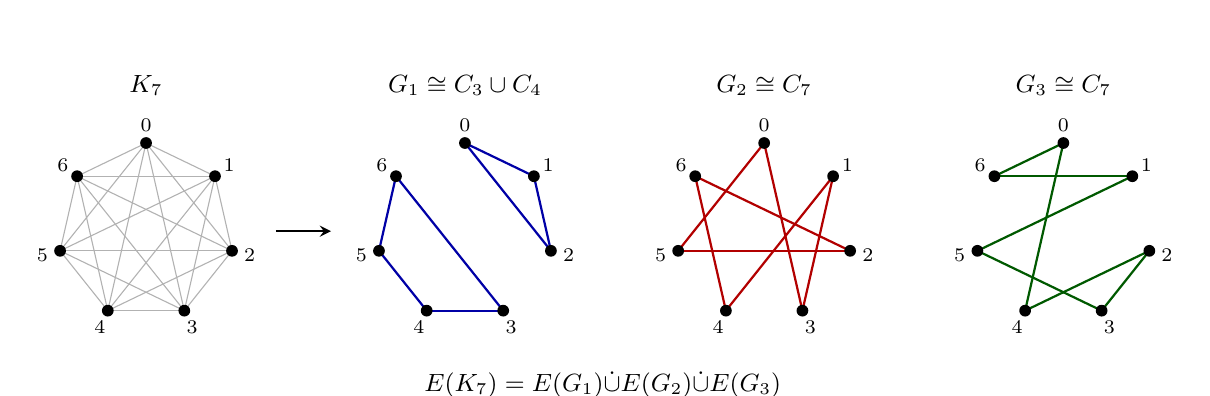
\begin{tikzpicture}[x=1cm,y=1cm,font=\small,>=stealth,
 dot/.style={circle,fill=black,inner sep=1.5pt},
 first/.style={blue!65!black,thick},
 second/.style={red!70!black,thick,dashed},
 shared/.style={green!35!black,very thick},
 spoke/.style={black!45,thin},
 tag/.style={fill=white,inner sep=1pt,font=\scriptsize}]
\begin{scope}[shift={(0,0)}]
\coordinate (n0) at (0.0000,1.1200);
\coordinate (n1) at (0.8757,0.6983);
\coordinate (n2) at (1.0919,-0.2492);
\coordinate (n3) at (0.4859,-1.0091);
\coordinate (n4) at (-0.4859,-1.0091);
\coordinate (n5) at (-1.0919,-0.2492);
\coordinate (n6) at (-0.8757,0.6983);
\draw[black!30,thin] (n0)--(n1);
\draw[black!30,thin] (n0)--(n2);
\draw[black!30,thin] (n0)--(n3);
\draw[black!30,thin] (n0)--(n4);
\draw[black!30,thin] (n0)--(n5);
\draw[black!30,thin] (n0)--(n6);
\draw[black!30,thin] (n1)--(n2);
\draw[black!30,thin] (n1)--(n3);
\draw[black!30,thin] (n1)--(n4);
\draw[black!30,thin] (n1)--(n5);
\draw[black!30,thin] (n1)--(n6);
\draw[black!30,thin] (n2)--(n3);
\draw[black!30,thin] (n2)--(n4);
\draw[black!30,thin] (n2)--(n5);
\draw[black!30,thin] (n2)--(n6);
\draw[black!30,thin] (n3)--(n4);
\draw[black!30,thin] (n3)--(n5);
\draw[black!30,thin] (n3)--(n6);
\draw[black!30,thin] (n4)--(n5);
\draw[black!30,thin] (n4)--(n6);
\draw[black!30,thin] (n5)--(n6);
\node[dot] at (n0) {};
\node[font=\scriptsize] at (0.0000,1.3500) {$ 0 $};
\node[dot] at (n1) {};
\node[font=\scriptsize] at (1.0555,0.8417) {$ 1 $};
\node[dot] at (n2) {};
\node[font=\scriptsize] at (1.3162,-0.3004) {$ 2 $};
\node[dot] at (n3) {};
\node[font=\scriptsize] at (0.5857,-1.2163) {$ 3 $};
\node[dot] at (n4) {};
\node[font=\scriptsize] at (-0.5857,-1.2163) {$ 4 $};
\node[dot] at (n5) {};
\node[font=\scriptsize] at (-1.3162,-0.3004) {$ 5 $};
\node[dot] at (n6) {};
\node[font=\scriptsize] at (-1.0555,0.8417) {$ 6 $};
\node at (0,1.85) {$K_7$};
\end{scope}
\begin{scope}[shift={(4.05,0)}]
\coordinate (n0) at (0.0000,1.1200);
\coordinate (n1) at (0.8757,0.6983);
\coordinate (n2) at (1.0919,-0.2492);
\coordinate (n3) at (0.4859,-1.0091);
\coordinate (n4) at (-0.4859,-1.0091);
\coordinate (n5) at (-1.0919,-0.2492);
\coordinate (n6) at (-0.8757,0.6983);
\draw[blue!65!black,thick] (n0)--(n1);
\draw[blue!65!black,thick] (n0)--(n2);
\draw[blue!65!black,thick] (n1)--(n2);
\draw[blue!65!black,thick] (n3)--(n4);
\draw[blue!65!black,thick] (n3)--(n6);
\draw[blue!65!black,thick] (n4)--(n5);
\draw[blue!65!black,thick] (n5)--(n6);
\node[dot] at (n0) {};
\node[font=\scriptsize] at (0.0000,1.3500) {$ 0 $};
\node[dot] at (n1) {};
\node[font=\scriptsize] at (1.0555,0.8417) {$ 1 $};
\node[dot] at (n2) {};
\node[font=\scriptsize] at (1.3162,-0.3004) {$ 2 $};
\node[dot] at (n3) {};
\node[font=\scriptsize] at (0.5857,-1.2163) {$ 3 $};
\node[dot] at (n4) {};
\node[font=\scriptsize] at (-0.5857,-1.2163) {$ 4 $};
\node[dot] at (n5) {};
\node[font=\scriptsize] at (-1.3162,-0.3004) {$ 5 $};
\node[dot] at (n6) {};
\node[font=\scriptsize] at (-1.0555,0.8417) {$ 6 $};
\node at (0,1.85) {$G_1\cong C_3\cup C_4$};
\end{scope}
\begin{scope}[shift={(7.85,0)}]
\coordinate (n0) at (0.0000,1.1200);
\coordinate (n1) at (0.8757,0.6983);
\coordinate (n2) at (1.0919,-0.2492);
\coordinate (n3) at (0.4859,-1.0091);
\coordinate (n4) at (-0.4859,-1.0091);
\coordinate (n5) at (-1.0919,-0.2492);
\coordinate (n6) at (-0.8757,0.6983);
\draw[red!70!black,thick] (n0)--(n3);
\draw[red!70!black,thick] (n0)--(n5);
\draw[red!70!black,thick] (n1)--(n3);
\draw[red!70!black,thick] (n1)--(n4);
\draw[red!70!black,thick] (n2)--(n5);
\draw[red!70!black,thick] (n2)--(n6);
\draw[red!70!black,thick] (n4)--(n6);
\node[dot] at (n0) {};
\node[font=\scriptsize] at (0.0000,1.3500) {$ 0 $};
\node[dot] at (n1) {};
\node[font=\scriptsize] at (1.0555,0.8417) {$ 1 $};
\node[dot] at (n2) {};
\node[font=\scriptsize] at (1.3162,-0.3004) {$ 2 $};
\node[dot] at (n3) {};
\node[font=\scriptsize] at (0.5857,-1.2163) {$ 3 $};
\node[dot] at (n4) {};
\node[font=\scriptsize] at (-0.5857,-1.2163) {$ 4 $};
\node[dot] at (n5) {};
\node[font=\scriptsize] at (-1.3162,-0.3004) {$ 5 $};
\node[dot] at (n6) {};
\node[font=\scriptsize] at (-1.0555,0.8417) {$ 6 $};
\node at (0,1.85) {$G_2\cong C_7$};
\end{scope}
\begin{scope}[shift={(11.65,0)}]
\coordinate (n0) at (0.0000,1.1200);
\coordinate (n1) at (0.8757,0.6983);
\coordinate (n2) at (1.0919,-0.2492);
\coordinate (n3) at (0.4859,-1.0091);
\coordinate (n4) at (-0.4859,-1.0091);
\coordinate (n5) at (-1.0919,-0.2492);
\coordinate (n6) at (-0.8757,0.6983);
\draw[green!35!black,thick] (n0)--(n4);
\draw[green!35!black,thick] (n0)--(n6);
\draw[green!35!black,thick] (n1)--(n5);
\draw[green!35!black,thick] (n1)--(n6);
\draw[green!35!black,thick] (n2)--(n3);
\draw[green!35!black,thick] (n2)--(n4);
\draw[green!35!black,thick] (n3)--(n5);
\node[dot] at (n0) {};
\node[font=\scriptsize] at (0.0000,1.3500) {$ 0 $};
\node[dot] at (n1) {};
\node[font=\scriptsize] at (1.0555,0.8417) {$ 1 $};
\node[dot] at (n2) {};
\node[font=\scriptsize] at (1.3162,-0.3004) {$ 2 $};
\node[dot] at (n3) {};
\node[font=\scriptsize] at (0.5857,-1.2163) {$ 3 $};
\node[dot] at (n4) {};
\node[font=\scriptsize] at (-0.5857,-1.2163) {$ 4 $};
\node[dot] at (n5) {};
\node[font=\scriptsize] at (-1.3162,-0.3004) {$ 5 $};
\node[dot] at (n6) {};
\node[font=\scriptsize] at (-1.0555,0.8417) {$ 6 $};
\node at (0,1.85) {$G_3\cong C_7$};
\end{scope}
\draw[->,thick] (1.65,0)--(2.35,0);
\node at (5.8,-1.95) {$E(K_7)=E(G_1)\dot\cup E(G_2)\dot\cup E(G_3)$};
\end{tikzpicture}
\caption{A decomposition into spanning factors with different cycle structures.
The same seven labeled vertices appear in every panel, and each edge of
$K_7$ occurs in exactly one of $G_1,G_2,G_3$.}
\label{fig:intro:prescribed-factors}
\end{figure}



Using the results mentioned in Section~\ref{subsec:cycle_decomp}, we obtain the following corollary.

\begin{corollary}\label{cor:new:factor-consequences}
For every $\alpha>0$, there exists $n_0=n_0(\alpha)$ such
that the following holds for every odd integer $L\ge3$ and
every $n\ge n_0$.
Let $F$ be an $n$-vertex $2$-factor, and let $G$
be a $D$-regular graph on $n$ vertices, where $D$ is even.
Then $G$ has an $F$-decomposition in each of the following cases.
\begin{enumerate}[label=\textup{(\roman*)}]
\item Every cycle of $F$ has length at least $L$, and
$D\ge(1/2 + 1/(2L-2)+\alpha)n$.
\item Every cycle of $F$ has even length, and
$D\ge(2/3+\alpha)n$.
\item Every cycle of $F$ has even length at least six, and
$D\ge(1/2+\alpha)n$.
\end{enumerate}
\end{corollary}

Corollary~\ref{cor:new:factor-consequences}(i), with $L=3$, gives
Conjecture~\ref{conj:gen_oberwolfach}(i).
Taking $L$ sufficiently large in the same corollary gives
Conjecture~\ref{conj:gen_oberwolfach}(iv).
Finally, Corollary~\ref{cor:new:factor-consequences}(ii),(iii)
give Conjecture~\ref{conj:gen_oberwolfach}(ii),(iii), respectively.

Let\phantomsection\label{gls:resolvable-cycle-decomposition-threshold} $\delta^{\rm res}_{C_r}$ be the infimum of $d \in [0,1]$ for which there exists $n_0 \in \mathbb{N}$ such that for all integers $n \geq n_0$ divisible by $r$, every $D$-regular graph on $n$ vertices with even $D \geq dn$ has a resolvable $C_r$-decomposition. 
Theorem~\ref{thm:new:prescribed-factor} implies Conjecture~\ref{conj:uniform_oberwolfach} as follows.

\begin{corollary}\label{cor:resolvable_threshold}
For every integer $r\ge3$,
$\delta^{\rm res}_{C_r}=\delta_{C_r}=\tau_r$.
\end{corollary}

The proofs of Theorem~\ref{thm:new:prescribed-factor} and
Corollaries~\ref{cor:new:factor-consequences} and~\ref{cor:resolvable_threshold}
are given in Section~\ref{sec:family:conclusion}.

\paragraph{Proof strategy for Theorem~\ref{thm:new:prescribed-factor}.}
Our proof combines the wheel encoding of prescribed factors due to
Keevash and Staden~\cite{KeevashStaden2022} with fractional decompositions
and iterative absorption~\cite{BarberEtAl2020Minimalist,BKLO2016,GlockThreshold2019,GlockEtAl2023Designs}.
We extend the original graph by adding one hub for each prescribed
factor, joined by spokes to every original vertex. A cycle together
with the spokes to a hub forms a wheel with that cycle as its rim.
The required factor decomposition is therefore equivalent to an
edge-decomposition of the extended graph into wheels with the
prescribed multiset of rim lengths at each hub.

The load of an edge is the sum of the weights of the wheels containing
it. Rim-edge and spoke loads record the use of each graph edge and of
each vertex in each prescribed factor, respectively.
For short cycles, we start from the balanced fractional cycle
decompositions supplied by Delcourt, Henderson, Lesgourgues and
Postle~\cite{DelcourtHendersonLesgourguesPostle2025}.
Distributing these weights over suitable hubs in the sampled extended
graph gives wheel weights whose rim-edge and spoke loads are close
to one. The weighted form of the Ehard--Glock--Joos matching
theorem~\cite{EGJ2020} given in Lemma~\ref{lem:new:weighted-resource-matching}
converts these weights into an approximate wheel
packing, leaving only a small proportion of the incident edges
uncovered at each original vertex and hub.
To obtain the smaller remainders required by the cover-down steps
below, we first remove a subgraph of small maximum degree to enforce
the rim--spoke degree identities. We then correct the weights on the
remaining graph to give load one on every rim edge and spoke, while
preserving positive lower and upper bounds of the required order.
The removed edges are covered later in the same cover-down step.

To obtain an exact wheel decomposition, we iterate the~\emph{cover-down lemmas} (Lemmas~\ref{lem:completion:ordinary-cover-down} and~\ref{lem:completion:marked-cover-down}) along a~\emph{vortex}, which is a nested sequence of pairs of vertex and hub sets, chosen to satisfy the required degree estimates at every level. In particular, the sizes of both vertex and hub sets decrease geometrically, ending with $O(1)$ graph vertices and $O(1)$ hubs.
Each application of the cover-down lemma first obtains an approximate
wheel packing from a fractional wheel decomposition.
Local constructions then extend this packing to cover every remaining
edge incident with a graph vertex or hub outside the next smaller pair. The local constructions use sufficiently few edges at each vertex and hub within the smaller pair to preserve the estimates needed for the next cover-down step.
The cover-down iteration leaves a remainder on the last vertex and hub sets of the vortex, each of size $O(1)$.
We absorb this remainder using an absorber chosen before the iteration of the cover-down lemma.

For long cycles, we follow the ideas of Keevash and Staden~\cite{KeevashStaden2022} in encoding paths with prescribed endpoints by wheels.
Their proof relies on the wheel-decomposition theorems~\cite[Theorems~3.1 and~3.3]{KeevashStaden2022}.
However, the extendability assumptions of these theorems do not follow from our minimum-degree hypothesis, so we obtain the required wheel decompositions by a different method.
To construct the required wheel weights, we use rapid mixing of
Markov chains, following Joos and K\"uhn~\cite{JK2022}, to obtain path
weightings with controlled endpoint distributions.
Brouwer's fixed-point theorem (Theorem~\ref{thm:prelim:brouwer}) then
makes these distributions compatible when the paths are joined into cycles.
The resulting cycle weightings have exact prescribed edge loads and quantitative positive weight bounds.
This construction supplies both the initial weights and the load corrections needed in the sampled graphs.
These load corrections and our absorbers yield the required wheel decomposition, completing the paths with their prescribed endpoints without reusing any edge of the original graph.
For a detailed proof overview, see Section~\ref{sec:writing:overview}.

The endpoint-matrix construction of
Section~\ref{sec:writing:cyclic-fractional}, combined with Brouwer's fixed-point theorem (Theorem~\ref{thm:prelim:brouwer}), also gives short proofs of fractional decomposition results of independent interest for cyclic-partite graphs.
These results and related conjectures are discussed in Section~\ref{subsec:intro:cyclic-fractional}.
In Section~\ref{sec:marked_cycle_weights}, we also give a short proof of the graph case ($k=2$) of Joos and K\"uhn's fractional cycle-decomposition theorem~\cite[Theorem~1.3]{JK2022}.
We expect these methods to have further interesting applications.


\begingroup
\let\subsection\frontsubsection
\clearpage
\section{Detailed overview of the proof of Theorem~\ref{thm:new:prescribed-factor}}
\label{sec:writing:overview}

Let $G$ be the $D$-regular graph in
Theorem~\ref{thm:new:prescribed-factor}, where $D$ is even, and let
$V:=V(G)$ and $n:=|V|$. The aim is to partition its edges into copies of
the prescribed spanning factors $F_1,\ldots,F_{D/2}$.

Following Keevash--Staden~\cite{KeevashStaden2022}, we first group
the prescribed factors according to their cycle lengths, relative
to a sufficiently large cutoff independent of $n$.
\begin{enumerate}[label=\textbf{Case \arabic*.},leftmargin=*]
\item \leavevmode\phantomsection\label{gls:ordinary-and-long-classes-of-factors}\textbf{A frequent bounded cycle length.}
Fewer than half the vertices of the factor lie in cycles above the
cutoff. Since there are only boundedly many lengths at most the
cutoff, cycles of some one length $r_*$ cover a positive proportion
of its vertices. Selecting one such length for each factor and
grouping factors with the same choice of $r_*$ defines the
\emph{ordinary classes}.
\item \textbf{A positive proportion of long cycles.}
At least half the vertices of the factor lie in cycles above the
cutoff. These factors form the \emph{long class}.
\end{enumerate}
A factor in an ordinary class may still contain long cycles.
There are only boundedly many classes. We embed the
factors in small classes separately and allocate a regular graph
to each remaining class, as explained in
Section~\ref{sec:overview:assembly}.

For\phantomsection\label{gls:complement-of-a-prescribed-factor} each remaining class, we reserve whole $r_*$-cycles in Case 1
and paths inside the long cycles in Case 2. The \emph{complement}
of a prescribed factor is the subgraph obtained by deleting its
reserved cycle components in Case 1, or the edges and internal
vertices of its reserved paths in Case 2. Thus, the endpoints of
reserved paths remain in the complement. We embed these complements
and then complete the reserved parts. 
In both Cases 1 and 2, the reserved cycles or paths can be chosen to cover a positive proportion of the vertices of every factor in the class.

Within a fixed class, let $U$ be a vertex set disjoint from $V$
indexing its prescribed $2$-factors, and denote the factor indexed
by $u\in U$ by $F_u$. Let $R$ be a graph on $V$ with $E(R)\subseteq E(G)$,
and let $H$ be a bipartite graph with parts $V,U$. We call
$(V,U,R,H)$ an \emph{extended graph}. The edges of $R$ are the
edges available for embedding cycles, and an edge $vu$ of $H$
allows $v$ to be used in factor $F_u$.

An \emph{$r$-wheel} consists of an $r$-cycle in $R$, called its
\emph{rim}, a vertex $u\in U$, called its \emph{hub}, and all
$r$ edges of $H$ joining $u$ to the rim vertices, called its
\emph{spokes} (see Figure~\ref{fig:overview:ordinary}).
Its rim gives a cycle in $G$ assigned to $F_u$.
In a packing of edge-disjoint wheels, the rim cycles are
edge-disjoint in $G$, and those assigned to the same factor are
vertex-disjoint because no spoke $vu$ can be used twice.
Thus, a wheel packing with the required rim lengths and multiplicities at each hub gives edge-disjoint embeddings of the corresponding cycle components of the prescribed factors.

\begin{figure}[htbp]
\centering
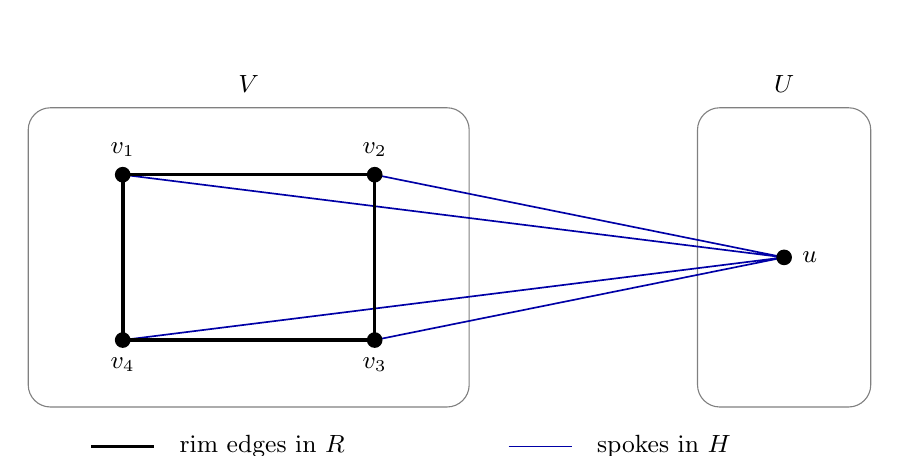
\begin{tikzpicture}[x=1cm,y=1cm,font=\small,
 v/.style={circle,fill=black,inner sep=2pt},
 spoke/.style={blue!65!black,semithick},
 rim/.style={black,line width=1.3pt}]
\draw[rounded corners=8pt,gray] (-6,-1.9) rectangle (-.4,1.9);
\draw[rounded corners=8pt,gray] (2.5,-1.9) rectangle (4.7,1.9);
\node at (-3.2,2.2) {$V$};
\node at (3.6,2.2) {$U$};
\coordinate (o1) at (-4.8,1.05);
\coordinate (o2) at (-1.6,1.05);
\coordinate (o3) at (-1.6,-1.05);
\coordinate (o4) at (-4.8,-1.05);
\coordinate (hub) at (3.6,0);
\draw[spoke] (o1)--(hub) (o2)--(hub) (o3)--(hub) (o4)--(hub);
\draw[rim] (o1)--(o2)--(o3)--(o4)--cycle;
\node[v,label=above:$v_1$] at (o1) {};
\node[v,label=above:$v_2$] at (o2) {};
\node[v,label=below:$v_3$] at (o3) {};
\node[v,label=below:$v_4$] at (o4) {};
\node[v,label=right:$u$] at (hub) {};
\draw[rim] (-5.2,-2.4)--(-4.4,-2.4);
\node[anchor=west] at (-4.2,-2.4) {rim edges in $R$};
\draw[spoke] (.1,-2.4)--(.9,-2.4);
\node[anchor=west] at (1.1,-2.4) {spokes in $H$};
\end{tikzpicture}
\caption{An ordinary $4$-wheel with rim vertices in $V$ and hub $u\in U$.
The thick rim is the image of a cycle of $F_u$, and the spokes record its vertices.
Edge-disjoint wheels at the same hub therefore have vertex-disjoint rims.}
\label{fig:overview:ordinary}
\end{figure}

The embedding has three stages. An approximate wheel packing first
embeds~\emph{most of the complement}, respecting the component
counts in each factor. We then embed~\emph{the rest of the
complement} greedily, extending the prescribed images and
preserving the edges reserved for completion. Finally,~\emph{iterative absorption} completes the reserved parts with
ordinary $r_*$-wheels or marked wheels of a fixed even length $c$.

Figure~\ref{fig:overview:plan} shows these three stages in the two
cases. We first explain the choice of reserved cycles or paths
and the marked representation, then describe how each stage is
carried out.

\begin{figure}[htbp]
\centering
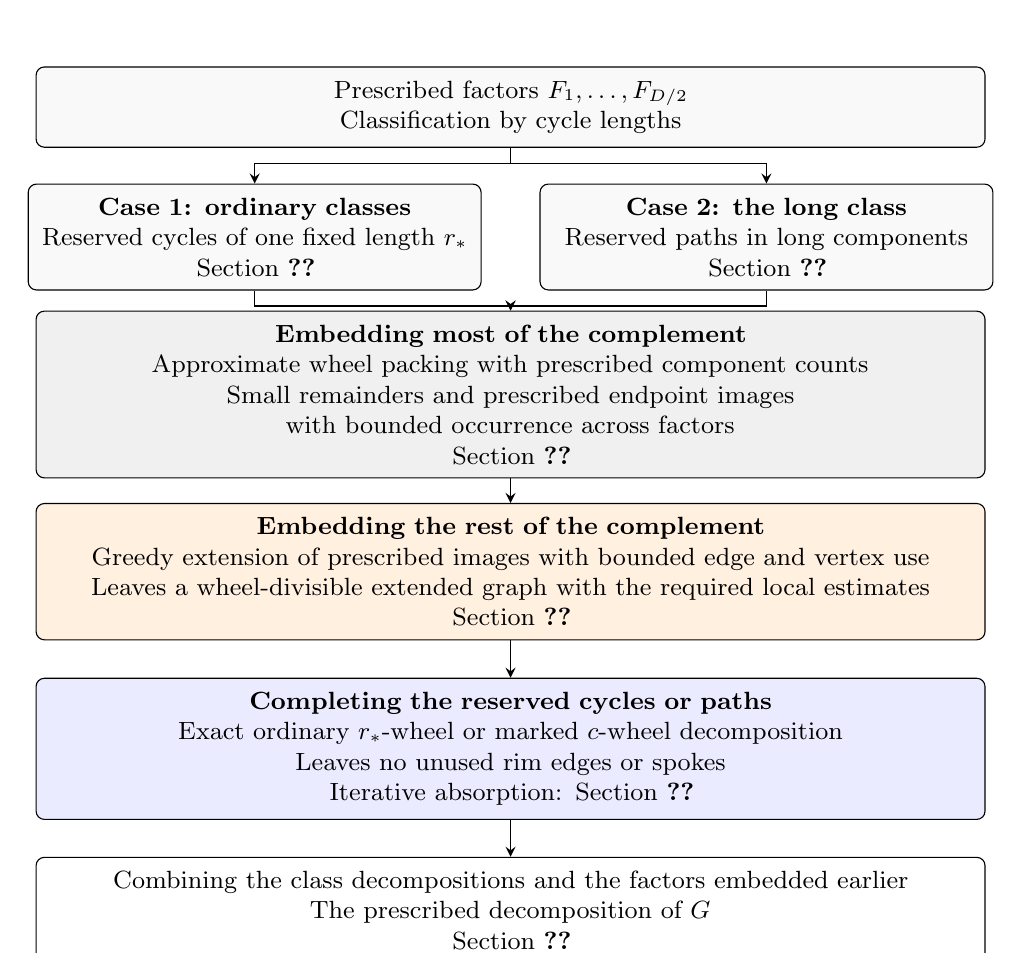
\begin{tikzpicture}[x=1cm,y=1cm,>=stealth,
 box/.style={draw,rounded corners=3pt,align=center,font=\small,
 inner sep=5pt,text width=5.4cm},arrow/.style={->,semithick}]
\node[box,text width=11.7cm,fill=gray!5] (all) at (0,0)
 {Prescribed factors $F_1,\ldots,F_{D/2}$\\Classification by cycle lengths};
\node[box,fill=gray!5] (ord) at (-3.25,-1.65)
 {\textbf{Case 1: ordinary classes}\\Reserved cycles of one fixed length $r_*$\\Section~\ref{sec:overview:reserved}};
\node[box,fill=gray!5] (mark) at (3.25,-1.65)
 {\textbf{Case 2: the long class}\\Reserved paths in long components\\Section~\ref{sec:writing:factor-overview}};
\draw[arrow] (all.south)--++(0,-.2)-|(ord.north);
\draw[arrow] (all.south)--++(0,-.2)-|(mark.north);
\node[box,text width=11.7cm,fill=gray!12] (most) at (0,-3.65)
 {\textbf{Embedding most of the complement}\\Approximate wheel packing with prescribed component counts\\Small remainders and prescribed endpoint images\\with bounded occurrence across factors\\Section~\ref{sec:overview:most-complement}};
\draw[arrow] (ord.south)--++(0,-.2)-|(most.north);
\draw[arrow] (mark.south)--++(0,-.2)-|(most.north);
\node[box,text width=11.7cm,fill=orange!12] (rest) at (0,-5.9)
 {\textbf{Embedding the rest of the complement}\\Greedy extension of prescribed images with bounded edge and vertex use\\Leaves a wheel-divisible extended graph with the required local estimates\\Section~\ref{sec:overview:rest-complement}};
\draw[arrow] (most)--(rest);
\node[box,text width=11.7cm,fill=blue!8] (complete) at (0,-8.15)
 {\textbf{Completing the reserved cycles or paths}\\Exact ordinary $r_*$-wheel or marked $c$-wheel decomposition\\Leaves no unused rim edges or spokes\\Iterative absorption: Section~\ref{sec:overview:completion}};
\draw[arrow] (rest)--(complete);
\node[box,text width=11.7cm] (end) at (0,-10.2)
 {Combining the class decompositions and the factors embedded earlier\\The prescribed decomposition of $G$\\Section~\ref{sec:overview:assembly}};
\draw[arrow] (complete)--(end);
\end{tikzpicture}
\caption{The three embedding stages in each of the two cases.
Gray, orange and blue indicate approximate packing, embedding the rest
of the complement, and completion, respectively, as in
Figure~\ref{fig:overview:three-embeddings}.
A prescribed list may contain classes of both kinds.}
\label{fig:overview:plan}
\end{figure}

We use the wheel encoding of Keevash--Staden~\cite{KeevashStaden2022}, but obtain the required wheel decompositions by different arguments.
Their wheel-decomposition theorems~\cite[Theorems~3.1 and~3.3]{KeevashStaden2022} follow from Keevash's general decomposition theorem~\cite{KeevashDesignsII2018}, whose application requires~\emph{extendability}: suitable small prescribed configurations must extend to the larger configurations used in the decomposition.
Our minimum-degree hypothesis does not imply this extendability condition. Instead, we use fractional cycle weights in the dense graph to obtain approximate wheel packings in sampled subgraphs.
For exact completion, we use iterative absorption along a~\emph{vortex}: a nested sequence of sets of graph vertices and factor indices.
Absorbers constructed in advance from suitable~\emph{transformers} are set aside during the iteration.
Each cover-down step covers the remaining edges outside the next pair of vertex sets.
The final remainder is supported on two sets of size $O(1)$ and is absorbed by the reserved absorbers.
Section~\ref{sec:overview:completion} explains this iteration and the construction of the absorbers.

\subsection{Case 1: a common bounded cycle length}
\label{sec:overview:reserved}

In each remaining ordinary class with chosen length $r_*$, the
same number of $r_*$-cycles is reserved in every factor. The other
components are embedded first (Figure~\ref{fig:overview:reserved-cycles}).
These components need not have bounded length. After their embedding, $R$ denotes the graph formed by the unused edges.

\begin{figure}[htbp]
\centering
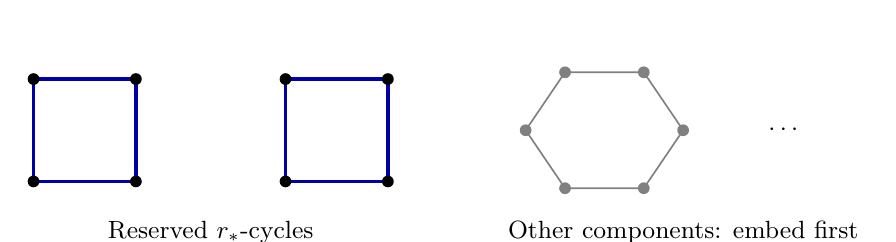
\begin{tikzpicture}[x=1cm,y=1cm,font=\small,
 v/.style={circle,fill=black,inner sep=1.5pt}]
\foreach \x/\name in {-4.6/a,-1.4/b} {
 \coordinate (\name1) at (\x-.65,-.65);
 \coordinate (\name2) at (\x+.65,-.65);
 \coordinate (\name3) at (\x+.65,.65);
 \coordinate (\name4) at (\x-.65,.65);
 \draw[blue!65!black,line width=1.3pt]
 (\name1)--(\name2)--(\name3)--(\name4)--cycle;
 \foreach \j in {1,2,3,4} {\node[v] at (\name\j) {};}
}
\foreach \j in {1,...,6} {
 \coordinate (d\j) at ({2+cos(60*\j)},{.85*sin(60*\j)});
}
\draw[gray,semithick] (d1)--(d2)--(d3)--(d4)--(d5)--(d6)--cycle;
\foreach \j in {1,...,6} {\node[v,fill=gray] at (d\j) {};}
\node at (4.3,0) {$\cdots$};
\node[align=center] at (-3,-1.3) {Reserved $r_*$-cycles};
\node[align=center] at (3,-1.3) {Other components: embed first};
\end{tikzpicture}
\caption{Case 1, illustrated with $r_*=4$. Selected cycles of the
common length are reserved (thick blue edges). The other components
are embedded before these cycles are completed.}
\label{fig:overview:reserved-cycles}
\end{figure}

Let $H$ be the bipartite graph of pairs $vu$ for which $v$ has not
been used by the embedding of the complement of $F_u$.
We construct the complement embeddings in Sections~\ref{sec:overview:most-complement}--\ref{sec:overview:preparation} so that the remaining extended graph $(R,H)$ satisfies the $r_*$-wheel divisibility conditions and retains the neighborhood, weighted-cycle and cut estimates required for completion.
Iterative absorption then yields an $r_*$-wheel decomposition of $(R,H)$, as described in Section~\ref{sec:overview:completion}.

\subsection{Case 2: a positive proportion of vertices in long cycles}
\label{sec:writing:factor-overview}

In the long class, we reserve several vertex-disjoint paths inside the long cycles, with lengths divisible by a fixed $c \in 2 \mathbb{N}$ chosen sufficiently large for the degree and density bounds. 
Since the endpoints of each reserved path belong to the complement, their images are fixed when the complement is embedded. We must then embed the reserved paths with these endpoint images and their prescribed lengths.
Along each prescribed cycle, consecutive reserved vertex-disjoint paths are separated by at least four vertices outside the reserved paths (see Figure~\ref{fig:overview:reserved-paths}).

\begin{figure}[htbp]
\centering
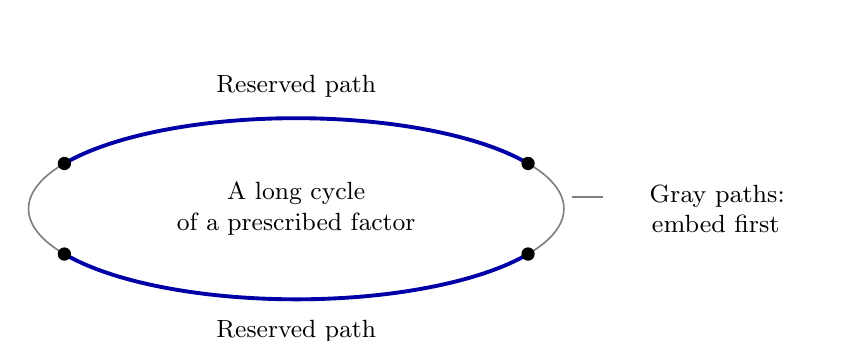
\begin{tikzpicture}[x=1cm,y=1cm,font=\small,
 v/.style={circle,fill=black,inner sep=1.7pt}]
\begin{scope}[xscale=3.4,yscale=1.15]
\draw[gray,semithick] (0,0) circle (1);
\draw[blue!65!black,line width=1.4pt] (30:1) arc (30:150:1);
\draw[blue!65!black,line width=1.4pt] (210:1) arc (210:330:1);
\end{scope}
\foreach \t in {30,150,210,330} {
 \node[v] at ({3.4*cos(\t)},{1.15*sin(\t)}) {};
}
\node at (0,1.55) {Reserved path};
\node at (0,-1.55) {Reserved path};
\node[align=center] at (0,0) {A long cycle\\of a prescribed factor};
\node[align=center,anchor=west,text width=2.4cm] at (4,.0)
 {Gray paths:\\embed first};
\draw[gray] (3.5,.15)--(3.9,.15);
\end{tikzpicture}
\caption{Reserved paths within one long cycle in Case 2 (thick blue).
Each has length divisible by $c$ and is completed using marked $c$-wheels.
The gray paths are embedded first, with prescribed images for the
shared endpoints (black dots).}
\label{fig:overview:reserved-paths}
\end{figure}

We use the successor encoding of Keevash--Staden~\cite{KeevashStaden2022}.
Glock, Joos, Kim, K\"uhn and Osthus~\cite{GlockEtAl2021Oberwolfach}
used a related but different rewiring method, recovering long
cycles from partite cycle factors in auxiliary graphs.
The encoding uses a permutation $\pi$ of $V$, chosen before
sampling with sufficiently long cycles and preserving the vertex
sets of the vortex described in Section~\ref{sec:overview:completion}. An auxiliary arc $x\to y$ has type $0$ (unmarked) or type $K$ (marked), recorded as $(x\to y,0)$ or $(x\to y,K)$, respectively. Its corresponding edge in the original graph $G$, called its~\emph{physical edge}, is given by
\begin{equation*}
 (x\to y,0)\longmapsto\{x,y\},\qquad
 (x\to y,K)\longmapsto\{x,\pi(y)\}.
\end{equation*}
Thus, marking the closing arc of the auxiliary cycle $x\to x_1\to\cdots\to x_{c-1}\to x$ gives a path $x,x_1,\ldots,x_{c-1},\pi(x)$ in the original graph $G$, provided $\pi(x)\notin\{x,x_1,\ldots,x_{c-1}\}$.

For distinct $x,x_1,\ldots,x_{c-1}\in V$, a marked $c$-wheel consists of the unmarked rim arcs $x\to x_1,\ldots,x_{c-2}\to x_{c-1}$, the marked rim arc $x_{c-1}\to x$, a hub $u\in U$, the marked spoke $xu$, and the unmarked spokes $x_i u$ for $1\le i\le c-1$.
For either type $j\in\{0,K\}$, the spoke $(xu,j)$ has physical edge $\{x,u\}$ in the extended graph.
In the marked wheel above, the type-$K$ spoke $xu$ records the initial vertex $x$ of the corresponding path in $G$.



\begin{figure}[htbp]
\centering
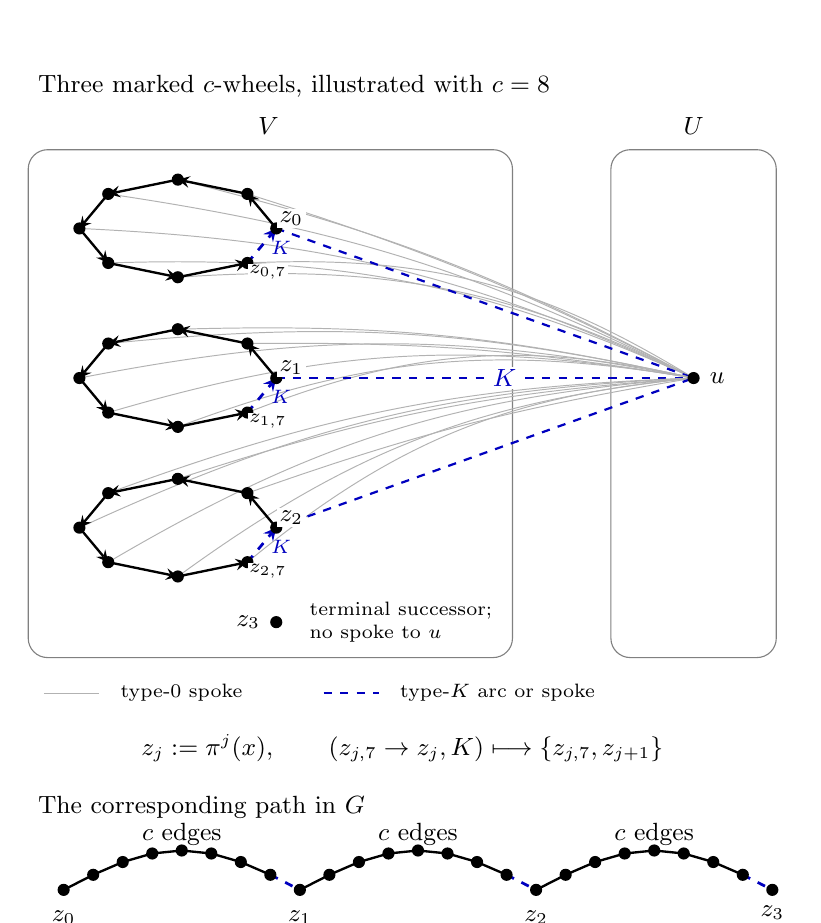
\begin{tikzpicture}[x=1cm,y=1cm,>=stealth,font=\small,
 v/.style={circle,fill=black,inner sep=1.55pt},
 rim/.style={->,line width=.85pt},
 spoke/.style={gray!60,line width=.35pt},
 markedrim/.style={->,blue!75!black,dashed,line width=1pt},
 markedspoke/.style={blue!75!black,dashed,line width=.8pt}]
\draw[rounded corners=7pt,gray] (-5.25,-3.55) rectangle (.9,2.9);
\draw[rounded corners=7pt,gray] (2.15,-3.55) rectangle (4.25,2.9);
\node at (-2.2,3.2) {$V$};
\node at (3.2,3.2) {$U$};
\node[anchor=west] at (-5.25,3.7) {Three marked $c$-wheels, illustrated with $c=8$};
\coordinate (hub) at (3.2,0);
% The three rims are vertex-disjoint; only the hub is shared.
\foreach \j/\yy in {0/1.9,1/0,2/-1.9} {
 \foreach \k in {0,...,7} {
  \coordinate (a\j\k) at ({-3.35+1.25*cos(45*\k)},{\yy+.62*sin(45*\k)});
 }
}
% Draw spokes behind the rim arcs. Curves avoid passing through rim vertices.
\foreach \j in {0,1,2} {
 \foreach \k in {1,...,7} {
  \draw[spoke] (a\j\k) to[bend left={3+2*\k}] (hub);
 }
 \draw[markedspoke] (a\j0)--(hub);
}
\foreach \j in {0,1,2} {
 \foreach \k [evaluate=\k as \next using int(\k+1)] in {0,...,6} {
  \draw[rim] (a\j\k)--(a\j\next);
 }
 \draw[markedrim] (a\j7)--node[right,pos=.45,font=\scriptsize] {$K$}(a\j0);
 \foreach \k in {0,...,7} {\node[v] at (a\j\k) {};}
 \node[anchor=south west,fill=white,inner sep=1pt] at (a\j0) {$z_\j$};
 \node[below right,font=\scriptsize,fill=white,inner sep=.5pt] at (a\j7) {$z_{\j,7}$};
}
\node[v,label=right:$u$] at (hub) {};
\node[blue!75!black,fill=white,inner sep=1pt] at (.8,0) {$K$};
\node[v,label=left:$z_3$] (terminal) at (-2.1,-3.1) {};
\node[anchor=west,font=\scriptsize,align=left] at (-1.8,-3.1) {terminal successor;\\no spoke to $u$};
\draw[spoke] (-5.05,-4)--(-4.35,-4);
\node[anchor=west,font=\scriptsize] at (-4.2,-4) {type-$0$ spoke};
\draw[markedspoke] (-1.5,-4)--(-.8,-4);
\node[anchor=west,font=\scriptsize] at (-.65,-4) {type-$K$ arc or spoke};
\node at (-.5,-4.7) {$z_j:=\pi^j(x),\qquad
 (z_{j,7}\to z_j,K)\longmapsto\{z_{j,7},z_{j+1}\}$};
\node[anchor=west] at (-5.25,-5.45) {The corresponding path in $G$};
% Each segment has seven internal vertices and eight physical edges.
\foreach \j in {0,1,2} {
 \foreach \k in {0,...,8} {
  \coordinate (p\j\k) at ({-4.8+3.0*\j+3.0*\k/8},{-6.5+.5*sin(180*\k/8)});
 }
 \foreach \k [evaluate=\k as \next using int(\k+1)] in {0,...,6} {
  \draw[line width=.85pt] (p\j\k)--(p\j\next);
 }
 \draw[blue!75!black,dashed,line width=1pt] (p\j7)--(p\j8);
 \foreach \k in {0,...,7} {\node[v] at (p\j\k) {};}
 \node[below=4pt] at (p\j0) {$z_\j$};
 \node at ({-3.3+3.0*\j},-5.8) {$c$ edges};
}
\node[v,label=below:$z_3$] at (p28) {};
\end{tikzpicture}
\caption{Successor encoding by three marked $c$-wheels at $u$, with $c=8$
and $z_j:=\pi^j(x)$. The marked closing arc of the rim starting at $z_j$
represents an edge to $z_{j+1}$ in $G$.
The three physical rims concatenate into the lower path of length $3c$,
whose dashed edges correspond to the marked arcs.
The terminal vertex $z_3$ has no spoke to $u$.}
\label{fig:overview:successor}
\end{figure}

For a fixed integer $d\ge2$, we call $I_a:=\{a,\pi(a),\ldots,\pi^{d-1}(a)\}$ a \emph{successor interval}, with \emph{terminal successor} $\pi^d(a)$ and \emph{extended interval} $I_a\cup\{\pi^d(a)\}$. At each hub, the extended intervals
have distinct vertices and are pairwise disjoint. The interval
vertices have marked spokes to that hub. In the extended subgraph
used to embed these paths, terminal successors have no spokes to
the hub, and all unmarked spoke neighbors lie outside the
extended intervals. 
A marked $c$-wheel decomposition therefore gives, at each hub $u$, one path segment of length $c$ in $G$ from $v$ to $\pi(v)$ for every vertex $v$ of an interval assigned to $u$.
Spoke disjointness makes their internal vertices distinct.
The segments meet only at successive interval vertices and form
a path from $a$ to $\pi^d(a)$ of length $cd$. Different intervals
at the same hub give vertex-disjoint paths, as in Figure~\ref{fig:overview:successor}.
No two wheels in this marked $c$-wheel decomposition use the same
physical rim edge of $G$ or the same spoke.
Lemma~\ref{lem:reconstruction:paths} proves this reconstruction.

The same encoding is used for approximately packing paths in the
long components of an ordinary class. 

\subsection{Embedding most of the complement}
\label{sec:overview:most-complement}

Let $P\subseteq G$ be the regular graph remaining after the factors in small classes have been embedded.
For a fixed remaining class, let $S$ be the regular spanning subgraph obtained by correcting the degrees in its part of a random partition of $E(P)$, as described in Section~\ref{sec:overview:assembly}.
The rim and spoke samples described below are chosen before this correction, which preserves the absorber and the inner induced subgraph reserved for completion.
Within $S$, an approximate wheel packing embeds most of each complement, using no more short cycles of any length than occur in that complement.

Short cycle components are embedded using unmarked wheels, whose rim arcs and spokes all have type $0$. Paths in long components are embedded using marked wheels.
In an ordinary class, a physical rim edge has no fixed type, and the marked closing arc is specified separately in each candidate marked wheel. The unembedded parts and their prescribed vertex images will be handled in the next stage.

\paragraph{Reservations for completion.}
Before sampling the rim edges and spokes, we fix small sets $I\subseteq V$ and $J\subseteq U$ on which part of the extended graph will be protected for completion. They form the first inner pair of the vortex described in Section~\ref{sec:overview:completion}.

The sampling procedure described below constructs an extended graph $\mathcal B$ for embedding the reserved
cycles or paths. Its rim edges within $I$ and spokes between $I$ and $J$ form $\mathcal B[I\cup J]$. For marked arcs, the restriction is by
auxiliary endpoints, and $\pi(I)=I$ also keeps their physical
endpoints in $I$.
After sampling and before either complement embedding, we reserve
an absorber $\mathcal A\subseteq\mathcal B$ with
$\mathcal A[I\cup J]=\varnothing$, as constructed in
Section~\ref{sec:overview:completion}. Thus $\mathcal A$ uses no rim
edge inside $I$ and no spoke between $I$ and $J$, although it may
meet $I\cup J$. Both complement embeddings preserve the edges
of $\mathcal A$ and $\mathcal B[I\cup J]$.

\paragraph{From wheel weights to a matching.}
The approximate packing is obtained from a matching in a hypergraph $\mathcal H$, where the vertices of $\mathcal H$ are the available physical rim edges and spokes, and each candidate wheel $W$ corresponds to an edge of $\mathcal H$ whose vertices are the physical rim edges
and spokes used by $W$.
For example, the auxiliary arcs $(x\to y,0)$ and $(x\to\pi^{-1}(y),K)$ both represent the edge $\{x,y\}$.
Wheels using either representation are therefore incident with the same vertex $\{x,y\}$ of $\mathcal H$.
A matching in $\mathcal H$ therefore corresponds to a collection of wheels with pairwise disjoint sets of physical rim edges and spokes.
Together with the interval conditions in Section~\ref{sec:writing:factor-overview}, this makes the cycle embeddings vertex-disjoint from one another and from the path embeddings at each hub. Two selected path segments at that hub can meet only at the common endpoint of consecutive segments.

To obtain an almost-perfect matching from the theorem of Ehard, Glock and Joos~\cite{EGJ2020} (Theorem~\ref{thm:prelim:weighted-matching}), we use nearly equal vertex degrees and codegrees much smaller than these degrees.
The minimum-degree condition on $P$ does not ensure these conditions for the unweighted hypergraph $\mathcal H$.
We instead assign a nonnegative weight $\omega(W)$ to each candidate wheel $W$. Writing $E_W$ for the set of
its physical rim edges and spokes, we arrange that $\sum_{W:\,e\in E_W}\omega(W)=1\pm\eta$ for all $e\in V(\mathcal H)$, where $\eta>0$ is sufficiently small. These sums are the weighted degrees of $\mathcal H$. Bounds on the individual wheel
weights also give $\sum_{W:\,e,f\in E_W}\omega(W)=O(1/n)$ whenever $e \ne f \in V(\mathcal H)$, so the weighted codegrees are small compared with the
weighted degrees.
Lemma~\ref{lem:new:weighted-resource-matching}, a weighted consequence of the Ehard--Glock--Joos theorem (Theorem~\ref{thm:prelim:weighted-matching}), then gives an almost-perfect matching with control of the uncovered incident edges and the numbers of selected cycle components.


\paragraph{Cycle weights before sampling.}
Before sampling the rim edges and spokes, we fix the following
fractional cycle weightings and weightings of successor-encoded paths.

For every bounded cycle length $r$ used in the packing, Theorem~\ref{thm:four:dense-spread} gives a fractional $C_r$-decomposition of $P$ in which every cycle has weight between positive constant multiples of $n^{2-r}$.
This theorem uses the result of Delcourt, Henderson, Lesgourgues and Postle~\cite{DelcourtHendersonLesgourguesPostle2025}.

For paths represented by marked $c$-wheels, we need weights on sequences $x_0,\ldots,x_{c-1}$ whose edges
\begin{equation*}
 x_0x_1,\ldots,x_{c-2}x_{c-1},
 x_{c-1}\pi(x_0)
\end{equation*}
belong to $P$. Here, $\operatorname{dist}_\pi$ denotes the shortest distance along a cycle of $\pi$, with distance $\infty$ between different cycles.
We restrict to sequences satisfying $\operatorname{dist}_\pi(x_i,x_j)>b$ for $i\ne j$, where $b\ge2$ is a fixed constant.
At each unmarked position, the total weight of sequences using a given ordered edge $xy$ of $P$ is close to one whenever $\operatorname{dist}_\pi(x,y)>b$.
At the closing position, the total weight of sequences with $x_{c-1}=x$ and $\pi(x_0)=y$ is close to one whenever $xy\in E(P)$ and $\operatorname{dist}_\pi(x,\pi^{-1}(y))>b$.
For sufficiently large even $c$, we obtain these weights by making
one copy of the vertex set at each cycle position and regularizing
the graphs between consecutive copies.
We combine the mixing argument of Joos and K\"uhn~\cite{JK2022}
with the path-joining construction of
Section~\ref{sec:writing:cyclic-fractional}.

We regard the required edge loads as capacities.
We divide the cyclic sequence of positions into three consecutive
blocks. On each block, mixing gives path weightings with prescribed
totals for each pair of endpoints, subject to fixed total weights
at the individual starting and ending vertices.
The fixed totals at individual endpoints are chosen in terms of the capacities so that the
path weights leave positive residual capacities and a second path
weighting, using half of each residual capacity, has the same
total weight as the first.

For each block, we require its prescribed endpoint-pair totals
to agree with those obtained by joining the second path weightings
on the other two blocks.
Brouwer's fixed-point theorem (Theorem~\ref{thm:prelim:brouwer}) gives simultaneous agreement for
all three blocks.
Taking each block in turn, we join its first path weighting to
the second weightings on the other two blocks.
The sum of the three resulting cycle weightings has exactly the
prescribed edge loads, with positive upper and lower bounds on
every cycle weight (Theorem~\ref{thm:four:long-capacities}).
Averaging over the regularizations and restricting to separated
tuples gives the required positional weights
(Theorem~\ref{thm:four:successor-kernel}).

\paragraph{Sampling and selecting wheels.}
We sample the rim edges and spokes for approximate packing and completion together, with probabilities reflecting the amounts to be embedded in each stage.
We use a variant of the~\textsc{Intervals} algorithm of Keevash--Staden~\cite[Section~4.1]{KeevashStaden2022} that samples fixed-length successor intervals $I_a$ whose extended intervals are pairwise disjoint at each hub.
At each hub of an ordinary class, successor intervals are sampled only for approximate packing.
At each hub of the single long class, two families of successor intervals are sampled jointly: one for
approximate packing and the other for embedding the reserved paths.

Each sampled interval $I_a$ assigned to a hub $u$ determines the marked spokes $vu$ for $v\in I_a$.
These spokes are assigned to approximate packing or to embedding the reserved paths according to the family containing $I_a$.
For each vertex $v$ outside all the extended intervals at $u$, a random label determines whether the spoke $vu$ is assigned to approximate packing, to completion, or to neither.
Spokes assigned to approximate packing in this way have type $0$. Those assigned to completion have no type in an ordinary class and have type $0$ in the long class.

We use all sampled completion intervals in the long class, leaving
their marked spokes unchanged. The marked degree identities are obtained
by adjusting the remaining rim-edge types after the complements have been
embedded, as described in Section~\ref{sec:overview:preparation}.
The sampling rules are given in Section~\ref{sec:four:local-intervals}.

For each factor $F_u$, let $m_{r,u}$ be the number of unreserved $r$-cycle components.
For each short length $r$ with sufficiently many unreserved components in $F_u$, we normalize the wheel weights so that the unmarked $r$-wheels at $u$ have total weight close to $(1-\theta)m_{r,u}$, where $\theta>0$ is small.
Short lengths with fewer unreserved components are handled when embedding the rest of the complement.
We assign a path in a long component of $F_u$ to each approximate-packing interval at $u$ and, in the long class, to each sampled completion interval at $u$.
Along each prescribed cycle, consecutive assigned paths are separated by at least four vertices outside these paths.

With high probability, every candidate unmarked rim cycle has
$\Omega(n)$ hubs joined to all its vertices by sampled type-$0$
spokes. We lift the cycle weights to wheel weights at these hubs,
taking account of the sampling probabilities, the numbers $m_{r,u}$,
and the numbers of vertices in the long components of each $F_u$.
A marked $c$-wheel uses one marked spoke and $c-1$ unmarked spokes. Thus, both wheel families contribute to the type-$0$ spoke loads, and their weights are normalized jointly. With high probability, the resulting loads on all available physical rim edges and spokes lie in $1\pm\eta$.
Each wheel of rim length $q$ has weight $O(n^{1-q})$. Any two distinct vertices of $\mathcal H$ belong together to at most $O(n^{q-2})$ candidate wheels of that length. Since only boundedly many lengths are used, the weighted codegrees of $\mathcal H$ are $O(1/n)$.

For a sufficiently small $0<\lambda<\theta$, Lemma~\ref{lem:new:weighted-resource-matching} gives a matching $M$ in $\mathcal H$ with the following properties.
Among the physical rim edges and spokes available for approximate packing, the corresponding wheel packing leaves at most $\lambda n$ rim edges unused at each $v\in V$ and at most $\lambda n$ spokes of each type unused at each $z\in V\cup U$.
For each short length $r$ treated at a hub $u$, the number of selected unmarked $r$-wheels lies in $(1-\theta\pm\lambda)m_{r,u}$.
Since $\lambda<\theta$, this number is at most $m_{r,u}$, so their rims can be assigned to distinct unreserved $r$-cycle components of $F_u$.

\paragraph{Unselected segments and prescribed endpoint images.}

The matching need not cover every marked spoke of an approximate-packing interval, so only some of its assigned path segments may be embedded at this stage.
For such an interval $I_a$ at $u$, let $y_0\cdots y_{cd}$ be its assigned path in $F_u$. We prescribe $y_{cj}\mapsto\pi^j(a)$ for every $0\le j\le d$.

For $0\le j<d$, a selected wheel whose marked spoke is $\pi^j(a)u$ embeds the segment $y_{cj}\cdots y_{c(j+1)}$ with these endpoint images.
Selected segments with consecutive indices concatenate at their prescribed common endpoints, as in Keevash--Staden~\cite[Lemma~7.1]{KeevashStaden2022}.
The unselected segments are embedded when we embed the rest of the complement.

The extended intervals at $u$ are pairwise disjoint, and the unmarked spoke neighbors of $u$ lie outside their union. Since the selected wheels use disjoint spokes, the prescribed endpoint images and the selected cycle and path embeddings together form an injective partial embedding of $F_u$.

If an endpoint of an unselected segment in $F_u$ is prescribed to have image $v$, then the marked spoke corresponding to that segment is either $vu$ or $\pi^{-1}(v)u$. The unused-spoke bound therefore gives
at most $2\lambda n$ endpoints of unselected segments with image $v$, counting across all factors.
Together with the bounds on interval starts and terminal successors, this bounds the number of prescribed endpoints mapped to each vertex. Since every factor has degree two, it also bounds the number of incident edges required there to extend these prescribed images when embedding the rest of the complement.

In the long class, each reserved path assigned to $I_a$ has prescribed
endpoint images $a$ and $\pi^d(a)$, while its internal vertices remain unembedded. The final marked $c$-wheel decomposition uses all marked spokes on every sampled completion interval, thereby embedding the reserved paths in full with these endpoint images.


\subsection{Embedding the rest of the complement}
\label{sec:overview:rest-complement}

For each $u$, let $Q_u$ be the remaining subgraph of the complement of $F_u$, retaining the vertices where it meets the selected or reserved paths. Each component of $Q_u$ is a path, an isolated vertex or a cycle.
The vertices $y_{cj}$ that remain in $Q_u$ already have prescribed images.

We extend these prescribed maps greedily to edge-disjoint embeddings of the graphs $Q_u$ in the available oriented graph, as illustrated in
Figure~\ref{fig:overview:three-embeddings}.
The embeddings are chosen so that the remaining extended graph on $I\cup J$ is exactly $\mathcal B[I\cup J]$ and every edge of $\mathcal A$ remains unused.
Moreover, the graph formed by all edges used at this stage, across all factors, has maximum degree at most a sufficiently small multiple of $n$. This bound preserves the estimates required for the final wheel decomposition.

We remark that this step is not a wheel decomposition. In particular, the terminal successor of a sampled completion interval has no spoke to its hub in either the approximate-packing or completion graph. Its prescribed vertex image is handled by the complement embedding.

\begin{figure}[htbp]
\centering
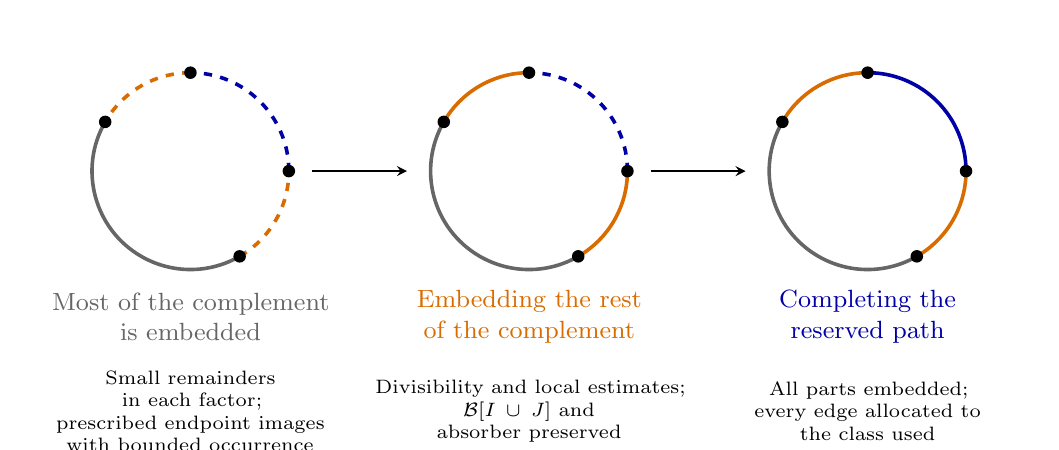
\begin{tikzpicture}[x=1cm,y=1cm,font=\small,>=stealth,
 used/.style={gray!80!black,line width=1.3pt},
 rest/.style={orange!85!black,line width=1.3pt},
 reserved/.style={blue!65!black,line width=1.3pt},
 v/.style={circle,fill=black,inner sep=1.6pt}]
\foreach \shift/\stage in {-4.3/1,0/2,4.3/3} {
 \begin{scope}[shift={(\shift,0)}]
  \draw[used] (150:1.25) arc (150:300:1.25);
  \ifnum\stage=1
   \draw[rest,dashed] (90:1.25) arc (90:150:1.25);
   \draw[rest,dashed] (300:1.25) arc (300:360:1.25);
  \else
   \draw[rest] (90:1.25) arc (90:150:1.25);
   \draw[rest] (300:1.25) arc (300:360:1.25);
  \fi
  \ifnum\stage=3
   \draw[reserved] (0:1.25) arc (0:90:1.25);
  \else
   \draw[reserved,dashed] (0:1.25) arc (0:90:1.25);
  \fi
  \foreach \t in {0,90,150,300} {\node[v] at (\t:1.25) {};}
 \end{scope}
}
\draw[->,semithick] (-2.75,0)--(-1.55,0);
\draw[->,semithick] (1.55,0)--(2.75,0);
\node[align=center,text width=3.9cm,text=gray!80!black] at (-4.3,-1.85)
 {Most of the complement\\is embedded};
\node[align=center,text width=3.9cm,text=orange!85!black] at (0,-1.85)
 {Embedding the rest\\of the complement};
\node[align=center,text width=3.9cm,text=blue!65!black] at (4.3,-1.85)
 {Completing the\\reserved path};
\node[align=center,text width=3.9cm,font=\scriptsize] at (-4.3,-3.05)
 {Small remainders in each factor;\\prescribed endpoint images\\with bounded occurrence};
\node[align=center,text width=3.9cm,font=\scriptsize] at (0,-3.05)
 {Divisibility and local estimates;\\$\mathcal B[I\cup J]$ and\\absorber preserved};
\node[align=center,text width=3.9cm,font=\scriptsize] at (4.3,-3.05)
 {All parts embedded;\\every edge allocated to\\the class used};
\end{tikzpicture}
\caption{Successive embeddings of one prescribed long cycle.
Gray, orange and blue indicate approximate packing, the rest of the
complement, and the reserved path, respectively. Each drawn arc
represents a path, with dashed arcs still unembedded.
The black junctions have prescribed images before the orange paths
are embedded. The lower annotations summarize the outputs for the
whole class of factors.}
\label{fig:overview:three-embeddings}
\end{figure}

\paragraph{The edges and images required for completion.}

Since all unprescribed vertex images will be chosen outside $I$,
every unused rim edge inside $I$ that is absent from $\mathcal B$
must be covered by an edge of some $Q_u$ whose endpoint images
are prescribed.
We also prescribe the use of the remaining rim edges excluded
by the $\pi$-separation conditions for completion.
All these required rim edges avoid the absorber $\mathcal A$.

We distribute the required edges among the factors indexed by
$U\setminus J$ so that each assigned set $M_u$ is a matching,
and put $M_u:=\varnothing$ for $u\in J$.
An edge $xy$ is assigned to $F_u$ only when neither endpoint
has already been used or prescribed as an image in $F_u$ and
the spokes $xu,yu$ of $\mathcal B$ are available outside
$\mathcal A$.
In the long class, these spokes must both have type $0$.
For each $u$, we choose a matching in $Q_u$ and prescribe its
image to be $M_u$, consistently with the vertex images already
fixed.

For $u\in J$, leaving precisely $\mathcal B[I\cup J]$ also requires
the complement embedding of $F_u$ to use every $v\in I$ for which
$vu\notin E(\mathcal B[I\cup J])$.
Any such vertex not already used or prescribed as an image in
$F_u$ is therefore prescribed as the image of an additional
vertex of $Q_u$.
The assignments are chosen so that each $v\in V$ occurs among
the prescribed images for at most a sufficiently small multiple
of $n$ factors.

We choose the positions of the additional prescribed vertices
in $Q_u$ so that the edges with both endpoint images prescribed
map precisely onto $M_u$.
All matchings $M_u$, including those assigned to factors that
will be embedded later, are reserved before any remaining
vertex images are chosen.

\paragraph{Extending the prescribed images.}
Let $\vec G_{\rm av}$ be the fixed oriented graph from which we choose edges not already prescribed, and let
$L_u$ be the set of allowed images for the unprescribed vertices of $Q_u$.
The set $L_u$ excludes $I$ and all images fixed for $F_u$ by the approximate packing and interval assignments.
It also excludes vertices joined to $u$ by an absorber spoke in an ordinary class, or by a type-$0$ absorber spoke in the long class.

For some fixed $\beta>0$, each $L_u$ is
$\beta$-extending in $\vec G_{\rm av}$
(Definition~\ref{def:lists:extending}).
In particular, $|N_{\vec G_{\rm av}}^\pm(x)\cap L_u|\ge\beta n$
for all $x\in V$, and $|N_{\vec G_{\rm av}}^+(x)\cap N_{\vec G_{\rm av}}^-(y)\cap L_u| \ge\beta n$ for all $x \ne y \in V$.
The minimum-degree bound on $P$, together with the sampling and stability estimates, gives these inequalities with high probability, simultaneously for every $u$ and every pair $x,y$. They therefore apply also to endpoint images chosen during the embedding.

Let $A_u$ be the set of vertices of $Q_u$ whose images have been prescribed.
We embed the components of $Q_u-A_u$ successively, using the one- and two-neighbor bounds above to extend these assignments.
When the last unembedded vertex of a path or cycle has predecessor and successor images $x\ne y$, its image is chosen from
$N_{\vec G_{\rm av}}^+(x)\cap N_{\vec G_{\rm av}}^-(y)\cap L_u$.
At each choice, we avoid images already prescribed or used in $F_u$, and require every new physical edge to avoid $\mathcal A$ and all edges already used or reserved for any factor.

\paragraph{Bounding the total use at each vertex.}
Let $\psi_u:A_u\to V$ be the prescribed map.
The preceding estimates give $|V(Q_u)|\le\delta n$ and $|\{u\in U:v\in\psi_u(A_u)\}|\le\delta n$ for all $v \in V$, where $\delta>0$ is sufficiently small compared with $\beta^2$.
The second bound includes the images prescribed by the interval assignments, the endpoints of the matchings $M_u$, and the additional prescribed images in $I$.

A vertex is excluded as a free image once it has been chosen freely
at least $\sqrt\delta\,n$ times across all factors.
Since there are at most $\delta n^2$ free choices, at most
$\sqrt\delta\,n$ vertices are excluded in this way.
The prescribed-image bound and $\Delta(Q_u)\le2$ then bound the maximum
degree of the edges prescribed or used at this stage by
$2\delta n+2\sqrt\delta\,n+2$.
These bounds, together with the bounded maximum degree of the absorber
$\mathcal A$, leave a positive number of choices in each extending
neighborhood after all forbidden vertices and edges are excluded.

Lemma~\ref{lem:new:prescribed-embedding} gives the resulting embeddings of the graphs $Q_u$. They agree with the prescribed maps and combine with the approximate packing to give edge-disjoint embeddings of all complements, while preserving $\mathcal A$.
The prescribed matchings and additional images in $I$, together with $L_u\cap I=\varnothing$, ensure that the remaining extended graph on $I\cup J$ is exactly $\mathcal B[I\cup J]$.
The bounds on edge use and vertex images control the changes in rim and spoke degrees required for completion.



\subsection{The remainder for exact completion}
\label{sec:overview:preparation}

At this point, every complement has been embedded. In the long class, these embeddings agree with the
prescribed endpoint images of the reserved paths.

For an ordinary class, let $S$ be its allocated $2|U|$-regular graph and let $R$ consist of the unused edges of $S$. Define the bipartite graph $H$ by
$vu\in E(H)$ if and only if the complement embedding of $F_u$ has not used $v$.
Each complement is a union of cycle components, so every occurrence of $v$ in a complement embedding uses
two edges incident with $v$.
Since $S$ is $2|U|$-regular and only whole $r_*$-cycles remain to be embedded at each hub, we have
\begin{equation*}
 d_R(v)=2d_H(v)\quad(v\in V),\qquad
 r_*\mid d_H(u)\quad(u\in U).
\end{equation*}
These are the $r_*$-wheel~\emph{divisibility conditions}.

In the long class, the allocated regular graph is given a balanced
orientation before the complements are embedded. The remaining physical
digraph need not be balanced, since the numbers of prescribed starts and
terminal successors at a vertex may differ. Let $H:=H^0\dot\cup H^K$
be the remaining spoke graph. We correct the types on a set of remaining
rim edges of small maximum degree, keeping their physical directions and
all spokes fixed. The target marked indegree at the physical vertex
$\pi(v)$ is $d_{H^K}(v)$, giving this same marked indegree at the
auxiliary vertex $v$. For the resulting auxiliary rim digraph
$R:=R^0\dot\cup R^K$, the prescribed endpoint images then give
\begin{align*}
 d_R^+(v)&=d_R^-(v)=d_H(v),\quad
 d_{R^K}^-(v)=d_{H^K}(v) &&(v\in V),\\
 d_{H^0}(u)&=(c-1)d_{H^K}(u) &&(u\in U).
\end{align*}
These are the marked $c$-wheel~\emph{divisibility conditions}.
At each hub, the marked spoke neighbors are precisely the vertices of its sampled completion intervals.
By the successor encoding, a marked $c$-wheel decomposition therefore reconstructs the reserved paths with their prescribed lengths and endpoint images.

The constructions preserve $\mathcal A$ and $\mathcal B[I\cup J]$.
The sampling estimates, together with the bounds on changes to rim edges and spokes, give the neighborhood, weighted-cycle and cut estimates needed for completion.
Section~\ref{sec:overview:completion} describes how iterative absorption yields the required wheel decompositions.
Together with the previous two stages of complement embedding, these decompositions prove Propositions~\ref{prop:family:ordinary-preparation} and~\ref{prop:family:long-preparation}.
Section~\ref{sec:overview:assembly} explains how the degree corrections needed to combine the classes preserve the hypotheses of these propositions.

\subsection{Completing the reserved parts by iterative absorption}
\label{sec:overview:completion}

We set aside the absorber $\mathcal A$ reserved before the complement
embeddings. Repeated approximate packings and cover-down steps cover
the remaining unused rim edges and spokes outside the final pair of
the vortex. The bounded terminal remainder is then absorbed by
$\mathcal A$.
The ordinary and marked cases have separate cover-down lemmas (Lemmas~\ref{lem:completion:ordinary-cover-down} and~\ref{lem:completion:marked-cover-down}) and absorber constructions.
The description below focuses on ordinary $r_*$-wheels, with the additional type constraints indicated for the marked case.

The iterative absorption method has its origins in work on Hamilton packings and decompositions~\cite{KnoxKuhnOsthus2015,KuhnOsthus2013Hamilton}.
It was developed for decompositions into a fixed graph in~\cite{BKLO2016,GlockThreshold2019} and for hypergraph
designs in~\cite{GlockEtAl2023Designs}. For an exposition in the setting of triangle decompositions,
see~\cite{BarberEtAl2020Minimalist}. Randomized variants have also been used to obtain threshold
results for designs and perfect matchings~\cite{SahSawhneySimkin2023,KangEtAl2023Latin,KangEtAl2024Matchings,PhamEtAl2022Toolkit}.

\paragraph{The vortex and the cover-down step.}
A~\emph{vortex} consists of nested pairs
\begin{equation*}
 (V,U)=(V_0,U_0)\supseteq(V_1,U_1)\supseteq\cdots\supseteq(V_\ell,U_\ell),
 \qquad (V_1,U_1)=(I,J),
\end{equation*}
with geometrically decreasing sizes and suitable degree conditions.
Both terminal sets $V_\ell$ and $U_\ell$ have bounded size. We put $V_{\ell+1}:=U_{\ell+1}:=\varnothing$.
The sets and $\pi$ are fixed before sampling, with $\pi(V_i)=V_i$ for every $i$. Thus, the successor of a vertex in $V_i$ also lies in $V_i$, and the successor encoding restricts to each level of the vortex.
At each level $0\le i<\ell$, the remainder has rim edges in $V_i$ and spokes between $V_i$ and $U_i$.
A~\emph{cover-down step} covers all rim edges with an endpoint outside $V_{i+1}$ and all spokes outside
$V_{i+1}\times U_{i+1}$. See Figure~\ref{fig:overview:vortex}.

\begin{figure}[!bp]
\centering
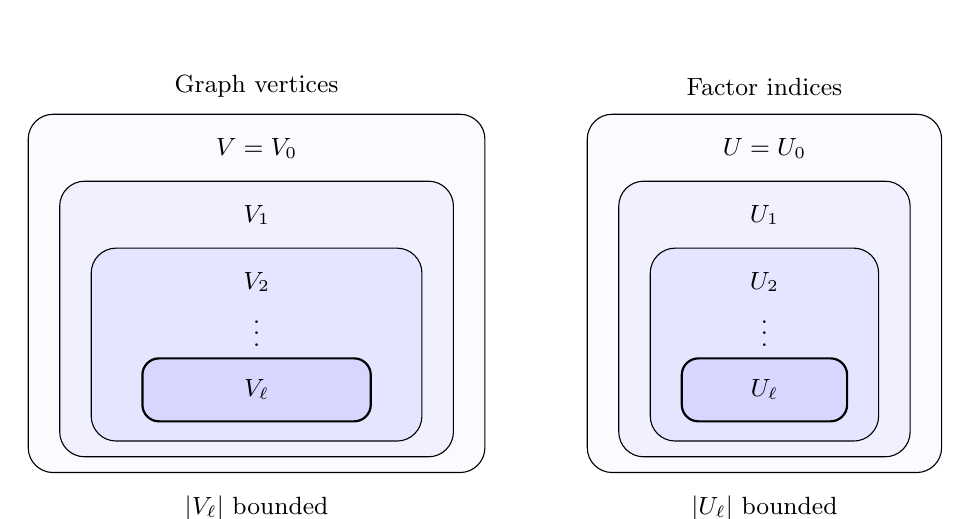
\begin{tikzpicture}[x=1cm,y=1cm,font=\small]
\node at (-3.4,4.9) {Graph vertices};
\node at (3.05,4.9) {Factor indices};
\draw[rounded corners=9pt,fill=blue!2] (-6.3,0) rectangle (-.5,4.55);
\draw[rounded corners=9pt,fill=blue!6] (-5.9,.2) rectangle (-.9,3.7);
\draw[rounded corners=9pt,fill=blue!10] (-5.5,.4) rectangle (-1.3,2.85);
\draw[rounded corners=6pt,thick,fill=blue!16] (-4.85,.65) rectangle (-1.95,1.45);
\node at (-3.4,4.12) {$V=V_0$};
\node at (-3.4,3.27) {$V_1$};
\node at (-3.4,2.42) {$V_2$};
\node at (-3.4,1.87) {$\vdots$};
\node at (-3.4,1.05) {$V_\ell$};
\draw[rounded corners=9pt,fill=blue!2] (.8,0) rectangle (5.3,4.55);
\draw[rounded corners=9pt,fill=blue!6] (1.2,.2) rectangle (4.9,3.7);
\draw[rounded corners=9pt,fill=blue!10] (1.6,.4) rectangle (4.5,2.85);
\draw[rounded corners=6pt,thick,fill=blue!16] (2,.65) rectangle (4.1,1.45);
\node at (3.05,4.12) {$U=U_0$};
\node at (3.05,3.27) {$U_1$};
\node at (3.05,2.42) {$U_2$};
\node at (3.05,1.87) {$\vdots$};
\node at (3.05,1.05) {$U_\ell$};
\node at (-3.4,-.45) {$|V_\ell|$ bounded};
\node at (3.05,-.45) {$|U_\ell|$ bounded};
\end{tikzpicture}
\caption{The two nested sequences of a vortex. At level $i$, rim edges lie within $V_i$ and spokes join $V_i$ to $U_i$. Both sets shrink until the terminal pair $(V_\ell, U_\ell)$ has bounded size.}
\label{fig:overview:vortex}
\end{figure}

\paragraph{Correcting the weights before approximate packing.}

Each cover-down step uses the approximate wheel-packing method of Section~\ref{sec:overview:most-complement}, where the approximate packing must leave a remainder of sufficiently small maximum degree for the local constructions that follow.
To find such an approximate packing, we use the matching lemma (Lemma~\ref{lem:new:weighted-resource-matching}) that requires the load error to be sufficiently small relative
to the desired bound on the uncovered degrees.
The initial load estimates do not guarantee this relation, since their tolerance is chosen before the remainder bound required by the subsequent local constructions.
We therefore correct the loads to one before applying the lemma, so that the matching error can be chosen sufficiently small for those constructions.

We first remove a subgraph of small maximum degree so that the
remaining graph satisfies the required rim--spoke degree identities
exactly. The removed edges are covered later in the same cover-down
step. We then correct the weights to obtain a fractional wheel
decomposition, with load one on every remaining physical rim edge
and spoke.

For ordinary $r_*$-wheels (Theorem~\ref{thm:pr:ordinary-wheel-weights}), we first lift signed cycle weightings to wheels to correct the rim-edge loads. We then transfer weight between hubs to correct the spoke loads while preserving every rim-edge load.

For marked wheels
(Theorem~\ref{thm:weights:marked-numerical}),
we correct the rim loads using fractional marked-cycle
decompositions with prescribed arc loads.
In the sampled graph, these loads need not be constant, and the
marked closing arcs may be much sparser than the unmarked arcs.
Theorem~\ref{thm:capacity:marked-numerical} obtains the required
marked-cycle weightings from
Theorem~\ref{thm:four:long-capacities}, using nonuniform locally
balanced capacities and imposing the mixing assumptions only
away from the marked closing position.
Excluding cycles with repeated or insufficiently separated original
labels introduces a small error in the arc loads.
Using the hyperplane separation theorem (Theorem~\ref{thm:prelim:separation}), we then obtain weights on the
remaining cycles with exactly the prescribed arc loads and
positive upper and lower bounds.
By lifting differences of these marked-cycle weightings to wheels,
we correct the rim loads.
We then correct the loads on spokes of both types while
preserving every rim load.

In both cases, the total change to each wheel weight is at most half the initial lower weight bound.
Thus, the corrected weights remain positive and, at a level with $N$ rim vertices, have order $N^{1-r_*}$ for ordinary wheels and $N^{1-c}$ for marked wheels.
As in Section~\ref{sec:overview:most-complement}, these weight bounds give weighted codegrees $O(1/N)$.


\paragraph{Covering the edges outside the next pair.}
Before approximate packing, we reserve subgraphs for the local constructions. After the approximate packing, we cover every remaining rim edge with both endpoints in $V_i\setminus V_{i+1}$ and every remaining spoke between $V_i\setminus V_{i+1}$ and $U_i\setminus U_{i+1}$.
The edges still incident with vertices outside $V_{i+1}\cup U_{i+1}$ are then covered by the following two constructions, illustrated in Figure~\ref{fig:overview:local-cover-down}.

We describe the ordinary case, writing $R$ and $H$ for the remaining rim and spoke graphs.
For each $u\in U_i\setminus U_{i+1}$, we have $N_H(u)\subseteq V_{i+1}$.
An $r_*$-cycle factor in $R[N_H(u)]$, together with the spokes at $u$, gives $r_*$-wheels covering all remaining spokes at that hub.

For each $v\in V_i\setminus V_{i+1}$, we have $N_R(v)\subseteq V_{i+1}$ and $N_H(v)\subseteq U_{i+1}$.
We pair the rim edges at $v$ and assign one pair to each spoke $vw$, choosing the assignment so that a pair $vx,vy$ assigned to $vw$ satisfies $x,y\in N_H(w)$.
The identity $d_R(v)=2d_H(v)$ ensures that the numbers of pairs and spokes agree.
A path of length $r_*-2$ from $x$ to $y$ in $R[V_{i+1}\cap N_H(w)]$, together with $vx,vy$ and the spokes to $w$, then forms an $r_*$-wheel.

Since both constructions use rim edges inside $V_{i+1}$,
we must coordinate the choice of cycle factors and endpoint
assignments.
Lemma~\ref{lem:new:bounded-degree-selection}, whose proof is
inspired by \cite[Lemma~3.10]{BarberEtAl2020Minimalist},
allows us to choose the cycle factors and the subgraphs
specifying these assignments with pairwise disjoint edge sets
and small maximum degree of their union.

When $r_*=3$, the selected subgraph for an endpoint assignment
already contains the closing edge $xy$.
For $r_*\ge4$, we reserve the assigned spokes $xw,yw$ and
complete the required paths greedily, avoiding both previously
used edges and edges reserved for other assignments.

The marked case follows the same division into cycle factors at hubs outside $U_{i+1}$ and paths through $V_{i+1}$ for rim vertices outside $V_{i+1}$.
The arc directions and the arc and spoke types are chosen to form marked $c$-wheels, whose physical rim edges and spokes are pairwise disjoint.
Lemmas~\ref{lem:completion:ordinary-cover-down} and~\ref{lem:completion:marked-cover-down} establish these cover-down steps in the ordinary and marked cases, respectively.

\begin{figure}[htbp]
\centering
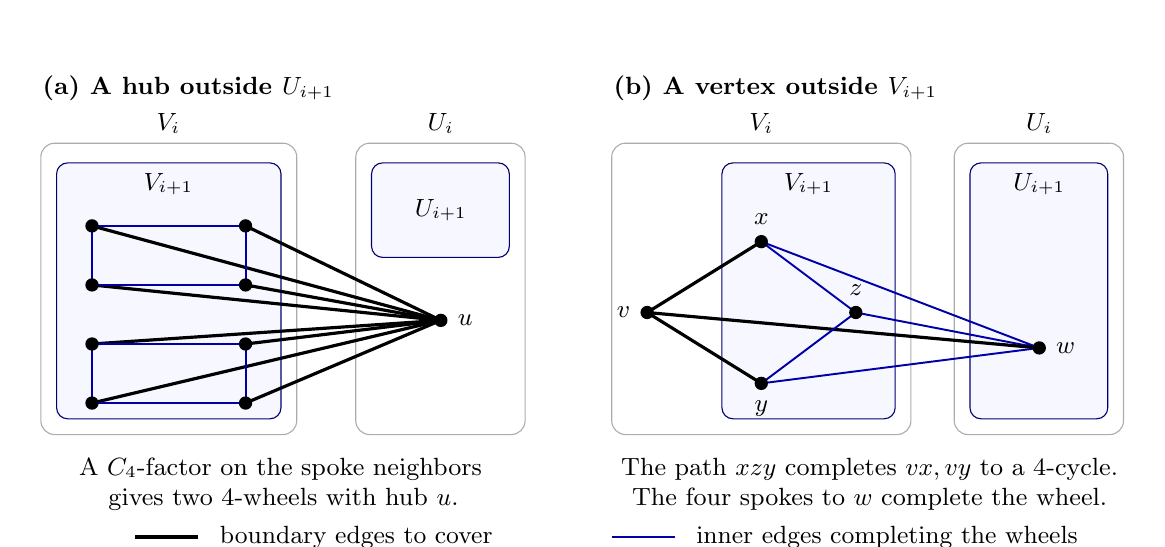
\begin{tikzpicture}[x=1cm,y=1cm,font=\small,
 vertex/.style={circle,fill=black,inner sep=1.7pt},
 outer/.style={rounded corners=5pt,draw=gray!65},
 inner/.style={rounded corners=4pt,draw=blue!45!black,fill=blue!3},
 boundary/.style={black,line width=1.15pt},
 added/.style={blue!65!black,line width=.7pt}]
\begin{scope}
 \node[anchor=west,font=\small\bfseries] at (-.1,2.85) {(a) A hub outside $U_{i+1}$};
 \draw[outer] (0,-1.55) rectangle (3.25,2.15);
 \draw[outer] (4.0,-1.55) rectangle (6.15,2.15);
 \node at (1.62,2.4) {$V_i$};
 \node at (5.08,2.4) {$U_i$};
 \draw[inner] (.2,-1.35) rectangle (3.05,1.9);
 \node at (1.62,1.63) {$V_{i+1}$};
 \draw[inner] (4.2,.7) rectangle (5.95,1.9);
 \node at (5.08,1.3) {$U_{i+1}$};
 \coordinate (hub) at (5.08,-.1);
 \coordinate (a1) at (.65,1.1);
 \coordinate (a2) at (2.6,1.1);
 \coordinate (a3) at (2.6,.35);
 \coordinate (a4) at (.65,.35);
 \coordinate (b1) at (.65,-.4);
 \coordinate (b2) at (2.6,-.4);
 \coordinate (b3) at (2.6,-1.15);
 \coordinate (b4) at (.65,-1.15);
 \foreach \z in {a1,a2,a3,a4,b1,b2,b3,b4}
   {\draw[boundary] (\z)--(hub);}
 \draw[added] (a1)--(a2)--(a3)--(a4)--cycle;
 \draw[added] (b1)--(b2)--(b3)--(b4)--cycle;
 \foreach \z in {a1,a2,a3,a4,b1,b2,b3,b4}
   {\node[vertex] at (\z) {};}
 \node[vertex,label=right:$u$] at (hub) {};
 \node[anchor=north,align=center,text width=6.2cm] at (3.05,-1.72)
   {A $C_4$-factor on the spoke neighbors\\gives two $4$-wheels with hub $u$.};
\end{scope}
\begin{scope}[xshift=7.25cm]
 \node[anchor=west,font=\small\bfseries] at (-.1,2.85) {(b) A vertex outside $V_{i+1}$};
 \draw[outer] (0,-1.55) rectangle (3.8,2.15);
 \draw[outer] (4.35,-1.55) rectangle (6.5,2.15);
 \node at (1.9,2.4) {$V_i$};
 \node at (5.43,2.4) {$U_i$};
 \draw[inner] (1.4,-1.35) rectangle (3.6,1.9);
 \node at (2.5,1.63) {$V_{i+1}$};
 \draw[inner] (4.55,-1.35) rectangle (6.3,1.9);
 \node at (5.43,1.63) {$U_{i+1}$};
 \coordinate (v) at (.45,0);
 \coordinate (x) at (1.9,.9);
 \coordinate (z) at (3.1,0);
 \coordinate (y) at (1.9,-.9);
 \coordinate (w) at (5.43,-.45);
 \draw[added] (x)--(w) (z)--(w) (y)--(w);
 \draw[boundary] (v)--(w);
 \draw[boundary] (v)--(x) (v)--(y);
 \draw[added] (x)--(z)--(y);
 \node[vertex,label=left:$v$] at (v) {};
 \node[vertex,label=above:$x$] at (x) {};
 \node[vertex,label=above:$z$] at (z) {};
 \node[vertex,label=below:$y$] at (y) {};
 \node[vertex,label=right:$w$] at (w) {};
 \node[anchor=north,align=center,text width=6.6cm] at (3.25,-1.72)
   {The path $xzy$ completes $vx,vy$ to a $4$-cycle.\\The four spokes to $w$ complete the wheel.};
\end{scope}
\draw[boundary] (1.2,-2.85)--(2,-2.85);
\node[anchor=west] at (2.15,-2.85) {boundary edges to cover};
\draw[added] (7.25,-2.85)--(8.05,-2.85);
\node[anchor=west] at (8.2,-2.85) {inner edges completing the wheels};
\end{tikzpicture}
\caption{The two local boundary constructions, illustrated with ordinary
$4$-wheels after approximate packing and the initial covering of
edges between outside vertices. In (a), $u\in U_i\setminus U_{i+1}$.
In (b), $v\in V_i\setminus V_{i+1}$ and $w\in U_{i+1}$.}
\label{fig:overview:local-cover-down}
\end{figure}


\paragraph{Preservation of the estimates along the vortex.}
To continue the iteration, the remainder must satisfy the completion estimates on the next pair, with the appropriate normalizations for its smaller vertex sets.
Recall that $\mathcal B$ is the extended graph constructed for completion in Section~\ref{sec:overview:most-complement}.
Let $\mathcal R_i$ be the remainder before the $i$th cover-down step, with the reserved absorber $\mathcal A$ excluded. At this stage, all rim edges and spokes of $\mathcal B[V_{i+1}\cup U_{i+1}]$ remain
unchanged, so $\mathcal R_i[V_{i+1}\cup U_{i+1}]=\mathcal B[V_{i+1}\cup U_{i+1}]$.

The maximum-degree bound on the edges used inside
$(V_{i+1},U_{i+1})$ controls the changes in the degree,
neighborhood and weighted-cycle estimates on domains whose
sizes are comparable to $|V_{i+1}|$.
It also preserves the cut estimates used for approximate packing.

The restricted balance and local estimates use normalizations
on smaller inner sets, so a degree loss that is small relative
to $|V_{i+1}|$ may still produce too large an error in these
estimates.
The cover-down lemmas (Lemmas~\ref{lem:completion:ordinary-cover-down} and~\ref{lem:completion:marked-cover-down}) therefore give a stronger maximum-degree
bound on the used edges incident with $V_{i+2}\cup U_{i+2}$,
including edges joining this deeper pair to the rest of
$(V_{i+1},U_{i+1})$.
This bound preserves the restricted balance and local estimates
after normalization by the sizes of the corresponding inner sets.

The identity for $\mathcal R_i[V_{i+1}\cup U_{i+1}]$ implies that
the estimates for the remainder on $(V_{i+1},U_{i+1})$ follow from the sampling estimates by accounting only for the edges removed in step $i$.
Step $i$ leaves the induced extended graph on $V_{i+2}\cup U_{i+2}$
unchanged, preserving the inner cut estimates and giving
$\mathcal R_{i+1}[V_{i+2}\cup U_{i+2}]=\mathcal B[V_{i+2}\cup U_{i+2}]$
for the next step.
Thus, the iteration proceeds with the same error bounds, as illustrated in Figure~\ref{fig:overview:nested}.

The sampling estimates are established simultaneously at every level and for every permitted choice of vertices and hubs, including those selected later in the construction.
The weighted cycle and path counts used in these estimates retain
the weights fixed before sampling. Edge deletion changes which
terms contribute, so we bound the total weight of the lost terms.
The corrected wheel weights are used separately for approximate packing.

\begin{figure}[htbp]
\centering
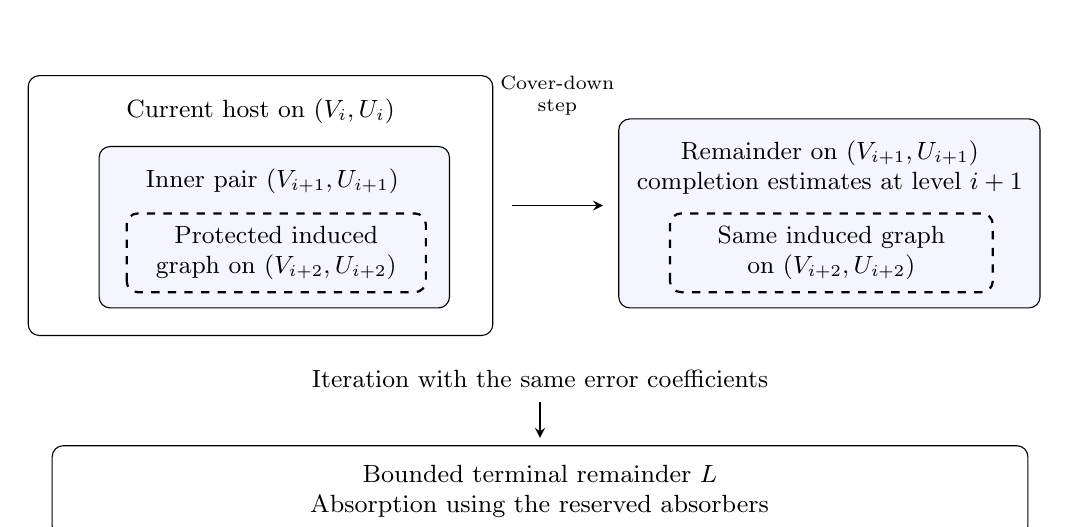
\begin{tikzpicture}[x=1cm,y=1cm,>=stealth,font=\small]
\draw[rounded corners] (-6.5,0) rectangle (-.6,3.3);
\draw[rounded corners,fill=blue!4] (-5.6,.35) rectangle (-1.15,2.4);
\draw[rounded corners,thick,dashed] (-5.25,.55) rectangle (-1.45,1.55);
\node at (-3.55,2.85) {Current host on $(V_i,U_i)$};
\node at (-3.4,1.96) {Inner pair $(V_{i+1},U_{i+1})$};
\node[align=center] at (-3.35,1.05) {Protected induced\\graph on $(V_{i+2},U_{i+2})$};
\draw[->,semithick] (-.35,1.65)--(.8,1.65);
\node[align=center,font=\scriptsize] at (.22,3.05) {Cover-down\\step};
\draw[rounded corners,fill=blue!4] (1,.35) rectangle (6.35,2.75);
\draw[rounded corners,thick,dashed] (1.65,.55) rectangle (5.75,1.55);
\node[align=center] at (3.68,2.13) {Remainder on $(V_{i+1},U_{i+1})$\\completion estimates at level $i+1$};
\node[align=center] at (3.7,1.05) {Same induced graph\\on $(V_{i+2},U_{i+2})$};
\node[align=center] at (0,-.55) {Iteration with the same error coefficients};
\draw[->,semithick] (0,-.85)--(0,-1.3);
\node[draw,rounded corners,align=center,inner sep=7pt,text width=11.9cm]
 at (0,-1.98) {Bounded terminal remainder $L$\\
 Absorption using the reserved absorbers};
\end{tikzpicture}
\caption{A cover-down step and terminal absorption.
The induced graph on $(V_{i+2},U_{i+2})$, shown dashed, is preserved.
Edge use has small maximum degree inside the next pair, with a stronger
bound for edges incident with $V_{i+2}\cup U_{i+2}$.
The terminal remainder is absorbed using absorbers reserved before
the iteration.}
\label{fig:overview:nested}
\end{figure}


\paragraph{Absorbing every possible terminal remainder.}
In\phantomsection\label{gls:ordinary-wheel-absorbers} the ordinary case, an $r_*$-wheel absorber for an extended graph $L$
is an extended graph $A_L$, edge-disjoint from $L$ and with each shared
vertex belonging to the rim parts of both graphs or to the hub parts of both,
such that $A_L[V(L)]=\varnothing$ and both $A_L$ and $A_L\cup L$
admit $r_*$-wheel decompositions.
Let $\mathcal L$ be the family of $r_*$-wheel-divisible extended subgraphs of $\mathcal B[V_\ell\cup U_\ell]$. Since $|V_\ell|$ and $|U_\ell|$ are bounded independently of $n$, so is $|\mathcal L|$.

After sampling and before embedding the complements, we reserve pairwise edge-disjoint absorbers $A_L\subseteq\mathcal B$ for all $L\in\mathcal L$, with $A_L[I\cup J]=\varnothing$.
Since $V_\ell\subseteq I$ and $U_\ell\subseteq J$, each absorber is edge-disjoint from every member of
$\mathcal L$.
The union $\mathcal A:=\bigcup_{L\in\mathcal L}A_L$ remains unused
throughout both complement embeddings and the iteration of the
cover-down lemmas.

When the iteration leaves a remainder
$L_{\rm fin}\in\mathcal L$, we combine an $r_*$-wheel decomposition of $A_{L_{\rm fin}}\cup L_{\rm fin}$ with an $r_*$-wheel decomposition of each $A_L$ for $L\ne L_{\rm fin}$.
Their union decomposes $\mathcal A\cup L_{\rm fin}$.
In the marked case, the same construction uses the family of marked $c$-wheel-divisible extended subgraphs of $\mathcal B[V_\ell\cup U_\ell]$ and marked $c$-wheel absorbers. No physical rim edge or spoke belongs to two absorbers, or to both an absorber and a possible terminal remainder.

The absorbers are constructed using~\emph{transformers}.
For\phantomsection\label{gls:ordinary-wheel-transformers} the ordinary case, let $T,L,L'$ be extended graphs with rim vertices in $V$ and hubs in $U$. Suppose that $L,L'$ are vertex-disjoint and that the three edge sets are pairwise disjoint.
We call $T$ an $r_*$-wheel transformer between $L$ and $L'$ if both $T\cup L$ and $T\cup L'$ admit $r_*$-wheel decompositions.
If $T[V(L)]=\varnothing$ and $L'$ itself admits such a decomposition, then $A_L:=T\cup L'$ is an absorber for $L$. Indeed, $A_L$ has the decomposition of $T\cup L'$, while a decomposition of $A_L\cup L$ is obtained by combining decompositions of $T\cup L$ and $L'$.
Figure~\ref{fig:overview:transformer} illustrates these two decompositions.
The transformer method was introduced by Barber, K\"uhn, Lo and Osthus~\cite[Section~8]{BKLO2016}
and developed further in~\cite{BKLOT2017,GlockThreshold2019,
BarberEtAl2020Minimalist,GlockEtAl2023Designs}.

Theorems~\ref{thm:new:ordinary-relative-absorber} and~\ref{thm:new:marked-relative-absorber} construct the required absorbers in the sampled extended graphs, with sizes bounded independently of $n$.
All vertices of $A_L$ outside $V(L)$ lie outside $I\cup J$, and $A_L[V(L)]=\varnothing$.
Since $V(L)\subseteq I\cup J$, these properties give $A_L[I\cup J]=\varnothing$.

The iteration of the cover-down lemmas and terminal absorption
together give the completion results,
Propositions~\ref{prop:completion:ordinary-construction}
and~\ref{prop:completion:marked-construction}.
Their wheel decompositions complete the embeddings of the reserved cycles in the ordinary classes and the reserved paths in the long class.

\begin{figure}[htbp]
\centering
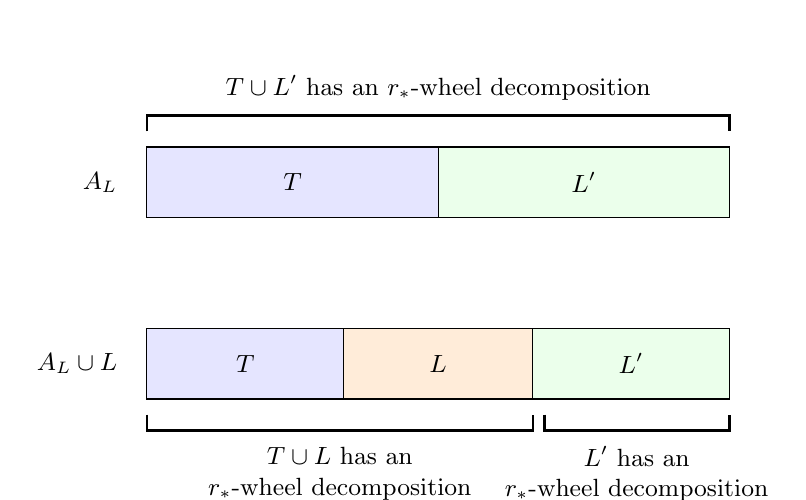
\begin{tikzpicture}[x=1cm,y=1cm,font=\small,>=stealth]
\node[anchor=east] at (-4.25,1.8) {$A_L$};
\draw[fill=blue!10] (-4,1.35) rectangle (-.3,2.25);
\draw[fill=green!8] (-.3,1.35) rectangle (3.4,2.25);
\node at (-2.15,1.8) {$T$};
\node at (1.55,1.8) {$L'$};
\draw[thick] (-4,2.45)--(-4,2.65)--(3.4,2.65)--(3.4,2.45);
\node at (-.3,3) {$T\cup L'$ has an $r_*$-wheel decomposition};
\node[anchor=east] at (-4.25,-.5) {$A_L\cup L$};
\draw[fill=blue!10] (-4,-.95) rectangle (-1.5,-.05);
\draw[fill=orange!15] (-1.5,-.95) rectangle (.9,-.05);
\draw[fill=green!8] (.9,-.95) rectangle (3.4,-.05);
\node at (-2.75,-.5) {$T$};
\node at (-.3,-.5) {$L$};
\node at (2.15,-.5) {$L'$};
\draw[thick] (-4,-1.15)--(-4,-1.35)--(.9,-1.35)--(.9,-1.15);
\draw[thick] (1.05,-1.15)--(1.05,-1.35)--(3.4,-1.35)--(3.4,-1.15);
\node[align=center] at (-1.55,-1.9)
 {$T\cup L$ has an\\$r_*$-wheel decomposition};
\node[align=center] at (2.22,-1.9)
 {$L'$ has an\\$r_*$-wheel decomposition};
\end{tikzpicture}
\caption{The two decompositions associated with the absorber $A_L=T\cup L'$.
The upper row decomposes $A_L$, while the lower row combines
decompositions of $T\cup L$ and $L'$ to decompose $A_L\cup L$.
The blocks represent pairwise edge-disjoint extended graphs.}
\label{fig:overview:transformer}
\end{figure}


\subsection{Combining the classes of prescribed factors}
\label{sec:overview:assembly}

We embed the factors in the small classes successively using Lemma~\ref{lem:family:single-copy}.
Each removal reduces every degree by two.
Since these classes contain at most a sufficiently small multiple of $n$ factors, the remaining graph $P$ is even-regular and retains the degree margin required by Propositions~\ref{prop:family:ordinary-preparation} and~\ref{prop:family:long-preparation}.

Let $D_0$ be the degree of $P$, and let $m_a$ be the number of factors in each remaining class $a$. Then $\sum_a m_a=D_0/2$.
We assign each edge of $P$ independently to a class, with probability $2m_a/D_0$ for class $a$.
For each $a$, let $S_a^0$ be the spanning subgraph consisting of the edges assigned to that class.
Thus, the sets $E(S_a^0)$ partition $E(P)$, and $\mathbb E\,d_{S_a^0}(v)=2m_a$ for every vertex $v$.
To obtain the prescribed decomposition in each class, we replace these sampled graphs by exactly $2m_a$-regular graphs.

Propositions~\ref{prop:family:ordinary-preparation} and~\ref{prop:family:long-preparation}
allow this degree correction while preserving the constructions needed for completion.
For each class $a$, a small inner set $I^{(a)}$ and a tolerance $\xi_a>0$ are fixed before sampling.
We choose a sampling outcome for which the conclusions of these propositions and Lemma~\ref{lem:family:partition} hold simultaneously.
The propositions supply edge sets $A_a\subseteq E(S_a^0)$, of total size bounded independently of $n$, such that every $2m_a$-regular spanning subgraph $S_a$ of $P$ satisfying
\begin{equation*}
 \Delta(S_a\triangle S_a^0)\le\xi_a n,\qquad
 S_a[I^{(a)}]=S_a^0[I^{(a)}],\qquad
 A_a\subseteq E(S_a)
\end{equation*}
admits a decomposition into the prescribed factors of class $a$.

Lemma~\ref{lem:family:partition} permits the sets $A_a$ to be selected after sampling, so it applies to these sets.
It reassigns edges between classes to produce a partition $E(P)=\dot\bigcup_a E(S_a)$ into $2m_a$-regular graphs satisfying the displayed conditions.
The proof adapts the random partition and degree correction in Keevash--Staden~\cite[proof of Lemma~9.1]{KeevashStaden2022}, while preserving the induced graphs $S_a^0[I^{(a)}]$ and the edge sets $A_a$.
The decompositions of the $S_a$, together with the factors already embedded from the small classes, give the required decomposition of $G$.




\paragraph{Organization.}
Sections~\ref{sec:main:reduction}--\ref{sec:family:conclusion} deduce
Theorem~\ref{thm:new:prescribed-factor} by combining decompositions for
the different classes of prescribed factors.
Part~\ref{part:common-tools} constructs fractional cycle and wheel
decompositions and derives approximate wheel packings.
Part~\ref{part:covering-absorbers} provides cycle factors and path
endpoint assignments for covering the boundary edges, and constructs
wheel absorbers using transformers.
Part~\ref{part:completion} uses sampling estimates and iterative
absorption to obtain ordinary and marked wheel decompositions for
completing the reserved cycles and paths.
Part~\ref{part:main-proof} embeds the complements so that the remaining
extended graphs admit these wheel decompositions. It also embeds
individual prescribed factors and constructs the regular edge partitions
used to combine the classes.
Section~\ref{sec:concluding} gives further fractional decomposition
results for cyclic-partite graphs. The appendices contain their proofs
and sharpness examples, together with the other proofs deferred from
the main text.


\section{Notation and terminology}

%We collect the graph, weighting and parameter conventions used below. Standard probabilistic, matching and convexity results are stated in Section~\ref{sec:preliminaries}.

\subsection{Sets, graphs and embeddings}

For an integer $k\ge0$, we write $[k]:=\{1,\ldots,k\}$, with $[0]:=\varnothing$.
We take $\mathbb N:=\{1,2,\ldots\}$ and use the standard notation
$\mathbb Z,\mathbb R$, $A\dot\cup B$, $A\triangle B$ and
$\binom{A}{k}$. Empty sums and products are zero and one,
respectively. All logarithms are natural.

All graphs are finite and simple unless stated otherwise.
In a multigraph, degrees count edge multiplicities, with each loop
contributing two. For a graph $G$, we write $V(G)$ and $E(G)$
for its vertex and edge sets, $|G|:=|V(G)|$, $e(G):=|E(G)|$,
and $\operatorname{Comp}(G)$ for its connected components, regarded
as subgraphs. We write $xy$ for the unordered edge $\{x,y\}$.
For a simple graph $G$, $v\in V(G)$ and $S\subseteq V(G)$, let
\begin{equation*}
 N_G(v):=\{x\in V(G):vx\in E(G)\},\qquad
 N_G(v;S):=N_G(v)\cap S,\qquad d_G(v;S):=|N_G(v;S)|.
\end{equation*}
We also write $d_G(v,S)$ for $d_G(v;S)$, and use
$d_G(v),\delta(G),\Delta(G)$ for the degree, minimum degree and
maximum degree. For $S\subseteq V(G)$, our common and union
neighborhood notation is
\begin{equation*}
 N_G(S):=\bigcap_{v\in S}N_G(v),\qquad
 \Gamma_G(S):=\bigcup_{v\in S}N_G(v).
\end{equation*}
The empty intersection is the ambient vertex set, and the empty
union is empty. The graph subscript is omitted only when the graph
has been specified. 
%In $|d_P(v;A)-d_*|\le\eta|A|$, the~\emph{degree parameter} $d_*$ is real and need not be an integer.

For $S\subseteq V(G)$, let $G[S]$ be the induced subgraph on $S$
and let $e_G(S):=e(G[S])$.
For disjoint $S,T\subseteq V(G)$, let $G[S,T]$ have vertex parts
$S,T$ and edge set $\{xy\in E(G):x\in S,\ y\in T\}$, and let
$e_G(S,T):=e(G[S,T])$.
If $F$ is a subgraph of $G$, then $G-F$ has vertex set $V(G)$
and edge set $E(G)\setminus E(F)$. For an edge set $D\subseteq E(G)$,
we similarly write $G-D$ for the spanning graph with edge set
$E(G)\setminus D$.
Deleting a vertex set also deletes its incident edges.
Unions, intersections and differences of graphs with specified
vertices refer to their edge sets unless stated otherwise.
For a family $\mathcal F$ of subgraphs, $\bigcup\mathcal F$
is their edge union, counting each edge once.
The~\emph{star} $E_G(v)$ is the set of edges incident to $v \in V(G)$.
The star at a vertex set contains all edges with at least one endpoint in that set, including edges leaving it.

An\phantomsection\label{gls:labeled-embeddings-of-absorber-templates:embedding-convention}~\emph{embedding} is an injective homomorphism. A~\emph{labeled copy} retains the embedding, including the images of all specified positions.
In typed or directed graphs, embeddings preserve the specified types and directions. A~\emph{rooted} graph has
specified vertices, called roots, whose images are prescribed. A~\emph{rooted embedding} is an embedding that extends that map. The other vertices are called~\emph{free}.

Paths and cycles are simple, and their lengths count edges.
We write $\mathcal C_r(G)$ for the copies of $C_r$ in $G$,
without a chosen orientation or starting point unless specified.
For\phantomsection\label{gls:part-respecting-cycles} specified cyclic vertex classes $V_0,\ldots,V_{r-1}$,
$\mathcal C_r^{\rm part}(G)$ denotes the cycles that use one vertex
from each class in this cyclic order.
A\phantomsection\label{gls:cycle-decomposition-and-resolvability:packings-factors}~\emph{packing} consists of edge-disjoint copies. A~\emph{factor}
consists of vertex-disjoint copies covering the specified vertex set.

\subsection{Asymptotic notation and hierarchies of constants}

We use the standard asymptotic notation $O,\Omega,o,\Theta$.
The implicit constants may depend only on the fixed parameters of
the relevant assertion. Subscripts specify dependencies when needed.
The\phantomsection\label{gls:interval-error-notation} notation $a\pm b$ means $[a-b,a+b]$, and equality to such
an expression asserts membership in that interval. In particular,
$(1\pm\epsilon)a=[(1-\epsilon)a,(1+\epsilon)a]$ for $a\ge0$.
An event holds \emph{with high probability} if its probability tends
to one as the graph order tends to infinity, with the stated constants
fixed. We write this probability as $1-o(1)$.

We\phantomsection\label{gls:hierarchy-of-constants} use $\ll$ to denote a hierarchy of constants, as follows.\footnote{This use of $\ll$ differs from its use for asymptotic comparison, such as $a=O(b)$.}
Let $\mathbf x_i=(x_{i,1},\ldots,x_{i,n_i})$ be a vector of
positive real parameters, where $n_i\ge1$ for $i\in[k]$.
The notation
\begin{equation*}
    0<x_{k,1},\ldots,x_{k,n_k} \ll x_{k-1,1},\ldots,x_{k-1,n_{k-1}} \ll\cdots\ll x_{1,1},\ldots,x_{1,n_1}
\end{equation*}
means that the parameters are chosen from right to left.
More precisely, there are positive functions
$\delta_i=\delta_i(\mathbf x_1,\ldots,\mathbf x_{i-1})$ for
$2\le i\le k$, each~\emph{nondecreasing} in every coordinate of
its arguments, such that the subsequent assertion holds for every
choice of $\mathbf x_1,\ldots,\mathbf x_k$ satisfying
$0<x_{i,j}\le\delta_i(\mathbf x_1,\ldots,\mathbf x_{i-1})$
for all $2\le i\le k$ and $j\in[n_i]$.

All parameters satisfy their stated domain restrictions, such as $p\in(0,1]$ and integrality of order parameters. 
When several hierarchies occur in one assertion, they are interpreted jointly. Their thresholds may also depend on parameters fixed earlier in the assertion, but are uniform over any subsequent inputs. 


\Needspace{7\baselineskip}
\subsection{Extended graphs, wheels and divisibility}
\label{sec:notation:wheels}

An\phantomsection\label{gls:extended-graph-ordinary-untyped} \emph{extended graph} is a tuple $\mathcal G=(V,U,G,H)$,
where $V,U$ are disjoint sets, $G$ is a simple graph on $V$,
and $H$ is a simple bipartite graph with parts $V,U$.
Its vertex set is $V(\mathcal G) := V \dot\cup U$, and its edge set is $E(\mathcal G) := E(G)\dot\cup E(H)$.
When the vertex parts are fixed, we also write $\mathcal G=(G,H)$.

An\phantomsection\label{gls:extended-subgraph-and-induced-restriction-ordinary} extended graph $\mathcal G'=(V',U',G',H')$ is an
\emph{extended subgraph} of $\mathcal G$ if $V'\subseteq V$,
$U'\subseteq U$, and both $G'$ and $H'$ are subgraphs of $G$
and $H$, respectively. We write $\mathcal G'\subseteq\mathcal G$.

Let\phantomsection\label{gls:wheel-rim-hub-and-spokes} $r\ge3$ be an integer. An \emph{$r$-wheel} consists of a cycle
of length $r$, called its \emph{rim}, a distinguished vertex outside
that cycle, called its \emph{hub}, and the $r$ edges joining the
hub to the cycle vertices, called its \emph{spokes}.
For $C\in\mathcal C_r(G)$ and $u\in U$ with
$V(C)\subseteq N_H(u)$, we write $W(C,u)$ for the wheel with
rim $C$, hub $u$, and spoke set $\{uv:v\in V(C)\}$.
An \emph{$r$-wheel in $\mathcal G$} is a wheel of this form.
Copies and embeddings preserve its distinguished hub and the roles of its rim edges and spokes.
A\phantomsection\label{gls:wheel-rim-hub-and-spokes:triangular}~\emph{triangular wheel} is a $3$-wheel, where its hub remains distinguished even though its underlying graph is $K_4$.

An\phantomsection\label{gls:ordinary-wheel-packings-and-decompositions} \emph{$r$-wheel packing} in $\mathcal G$ is a family of
edge-disjoint $r$-wheels in $\mathcal G$. It is an~\emph{$r$-wheel decomposition} if their edge sets partition
$E(\mathcal G) = E(G)\dot\cup E(H)$. We call $\mathcal G$ \emph{$r$-wheel-decomposable}
when it has such a decomposition. Identifying $W(C,u)$ with $(C,u)$, we define
\begin{equation*}
\mathcal W_r^{\rm ord}(\mathcal G):=\mathcal W_r(\mathcal G) := \{(C,u):C\in\mathcal C_r(G),\ u\in U,\ V(C)\subseteq N_H(u)\}.
\end{equation*}
A\phantomsection\label{gls:ordinary-wheel-packings-and-decompositions:fractional}~\emph{fractional $r$-wheel decomposition} is a function
$\omega:\mathcal W_r(\mathcal G)\to\mathbb R_{\ge0}$ satisfying
\begin{equation*}
 \sum_{\substack{W\in\mathcal W_r(\mathcal G)\\e\in E(W)}}\omega(W)=1
 \qquad(e\in E(G)\dot\cup E(H)).
\end{equation*}

We\phantomsection\label{gls:ordinary-wheel-divisibility} call $\mathcal G$~\emph{$r$-wheel-divisible} if $d_G(v)=2d_H(v)$ for all $v \in V$ and $r\mid d_H(u)$ for all $u \in U$, where these conditions are necessary for an $r$-wheel decomposition. We say that $\mathcal G=(V,U,G,H)$ is~\emph{$r$-wheel-divisible at $x\in V\cup U$} if
$d_G(x)=2d_H(x)$ when $x\in V$, and
$r\mid d_H(x)$ when $x\in U$.

For\phantomsection\label{gls:extended-subgraph-and-induced-restriction-ordinary:induced} $S\subseteq V\cup U$, the induced extended subgraph $\mathcal G[S]$
retains the vertices in $S$ and the rim edges and spokes with both
endpoints in $S$. In particular, for $A\subseteq V$ and $B\subseteq U$, we have $\mathcal G[A\cup B]=(A,B,G[A],H[A,B])$.
For an extended subgraph $\mathcal G'=(V',U',G',H')\subseteq\mathcal G$,
we use the same notation, with vertex parts $S\cap V'$ and $S\cap U'$.
The equality $\mathcal G'[S]=\varnothing$ means that this restriction has no edges, so its vertex parts are not necessarily empty.

\emph{Total degrees} in an extended graph $\mathcal G=(V,U,G,H)$ are
\begin{equation*}
 d_{\mathcal G}(x):=
 \begin{cases}d_G(x)+d_H(x),&x\in V,\\d_H(x),&x\in U.
 \end{cases}
\end{equation*}
Its maximum degree is the maximum of these total degrees.

Let $V_L$ and $U_L$ denote the rim and hub vertex sets of an
extended graph $L$. An embedding $\phi:L\to L'$ maps $V_L$ into
$V_{L'}$ and $U_L$ into $U_{L'}$, preserving the edges of each
component and all specified directions and types.

\subsection{Directed graphs, types and successor permutations}

For a directed graph $J$, we write $x\to y$, or $xy$, for
an arc with tail $x$ and head $y$, and we define
\begin{equation*}
 N_J^+(x):=\{y:x\to y\in E(J)\},\qquad
 N_J^-(x):=\{y:y\to x\in E(J)\},\qquad
 N_J^\pm(S):=\bigcap_{x\in S}N_J^\pm(x).
\end{equation*}

For $x\in V(J)$, the outdegree $d_J^+(x)$ and indegree $d_J^-(x)$
count arcs with tail $x$ and head $x$, respectively.
A directed graph is~\emph{balanced} if $d_J^+(v)=d_J^-(v)$ for
every vertex. For $S\subseteq V(J)$, let $N_J^\pm(x;S):=N_J^\pm(x)\cap S$.
The degrees $d_J^+(x;S)$ and $d_J^-(x;S)$ count, respectively, arcs from $x$ to $S$ and from $S$ to $x$, with multiplicity. When parallel arcs are allowed, degrees count multiplicity and neighborhoods are sets.

For\phantomsection\label{gls:bipartite-representation-of-a-digraph} a directed multigraph $R$, its bipartite representation is
$D_R:=(V(R)_{\rm out},V(R)_{\rm in};E_R)$, on two labeled copies of $V(R)$.
Its edges are indexed by the arcs of $R$, with the bijection
\begin{equation}
 \beta_R:E(R)\longrightarrow E_R,\qquad
 \beta_R(e):=x_{\rm out}y_{\rm in}\quad\text{if $e$ has tail $x$ and head $y$}.
 \label{eq:digraph:bipartite-representation}
\end{equation}
Parallel arcs give distinct indexed edges of $D_R$.
Here, $x_{\rm out}$ and $x_{\rm in}$ denote the tail and head copies of $x$.
For $S\subseteq V(R)$, let $S_{\rm out}:=\{x_{\rm out}:x\in S\}$
and $S_{\rm in}:=\{x_{\rm in}:x\in S\}$.

A~\emph{color} or~\emph{type} is an edge label, with no proper coloring requirement unless stated. 
We write $J^j$ for the subgraph of edges of type $j$.
Sampling a subgraph with probability $p$ means independent Bernoulli edge indicators with parameter $p$, unless a
different joint law is specified.

We extend the cyclic distance used by Keevash and Staden~\cite[Definition~3.2]{KeevashStaden2022} to permutations and use a strict inequality in the definition of separation.

\begin{definition}[Permutation distance and separation]\label{gls:permutation-distance-and-separation}
\label{def:new:permutation-intervals}
Let $b\ge0$ be an integer, let $V$ be finite, and let $\pi:V\to V$
be a permutation. The \emph{$\pi$-distance} between $x,y\in V$ is
\begin{equation*}
 \operatorname{dist}_\pi(x,y):=\min\{|k|:k\in\mathbb Z,\ \pi^k(x)=y\},
 \qquad\min\varnothing:=\infty.
\end{equation*}
A set $S\subseteq V$ is \emph{$(b,\pi)$-separated} if
$\operatorname{dist}_\pi(x,y)>b$ for all distinct $x,y\in S$.
A tuple is $(b,\pi)$-separated if its entries are distinct and its entry set
is $(b,\pi)$-separated. The sets $S,T\subseteq V$ are $(b,\pi)$-separated from each other if $\operatorname{dist}_\pi(x,y)>b$ for every $(x,y)\in S\times T$.
\end{definition}

We\phantomsection\label{gls:shortest-permutation-cycle-and-separation-graph} define $L_\pi := \min\{|C|:C\text{ is a cycle of }\pi\}$, where $L_\pi := \infty$ if $V=\varnothing$.
For $A\subseteq V$ and $x,y\in A$, the distance $\operatorname{dist}_\pi(x,y)$ is computed using $\pi$ on $V$, even though the intermediate iterates of $\pi$ need not lie in $A$.

Let\phantomsection\label{gls:shortest-permutation-cycle-and-separation-graph:separation-graph} $F_{\pi,b}$ be the graph on $V$ with $E(F_{\pi,b}):=\{xy\in\textstyle\binom{V}{2}: \operatorname{dist}_\pi(x,y)\le b\}$. Then $\Delta(F_{\pi,b})\le2b$, and a set $S\subseteq V$ is $(b,\pi)$-separated if and only if $F_{\pi,b}[S]$
is edgeless.


\subsection{Hypergraphs, fractional matchings and fractional decompositions}

A\phantomsection\label{gls:indexed-hypergraphs-and-incidence-map} finite multihypergraph is a triple
\begin{equation*}
 \mathcal H=(V(\mathcal H),E(\mathcal H),\iota_{\mathcal H}), \qquad \iota_{\mathcal H}:E(\mathcal H)\to 2^{V(\mathcal H)}\setminus\{\varnothing\},
\end{equation*}
where the vertex and edge sets are finite. Throughout, hypergraphs
may have~\emph{parallel} edges: distinct edges $h,h'$ are parallel if
$\iota_{\mathcal H}(h)=\iota_{\mathcal H}(h')$.
A hypergraph is~\emph{simple} if its incidence map is injective. In that
case its edges may be identified with their incident vertex sets.
We omit the subscript on $\iota_{\mathcal H}$ when the hypergraph is fixed.
It is~\emph{$r$-uniform} if $|\iota(h)|=r$ for every edge, and has~\emph{rank} at most $r$ if $|\iota(h)|\le r$ for every edge.

For $v\in V(\mathcal H)$ and distinct $u,v\in V(\mathcal H)$, we define the~\emph{degree} of $v$ and the~\emph{codegree} of a vertex-pair $\{u,v \}$ as follows:
\begin{equation*}
 d_{\mathcal H}(v):= |\{h\in E(\mathcal H):v\in\iota(h)\}|, \qquad d_{\mathcal H}(u,v):=|\{h\in E(\mathcal H):\{u,v\}\subseteq\iota(h)\}|.
\end{equation*}
Thus, degrees and codegrees count parallel edges separately.
We define the~\emph{maximum degree} $\Delta(\mathcal H) := \max_v d_{\mathcal H}(v)$ and the~\emph{maximum codegree} $\Delta_2(\mathcal H) := \max_{u\ne v}d_{\mathcal H}(u,v)$, where a maximum over an empty set is taken to be zero.
A~\emph{matching} is a set $M\subseteq E(\mathcal H)$ such that $\iota(h)\cap\iota(h')=\varnothing$ for distinct $h,h'\in M$. We define $V(M) := \bigcup_{h\in M}\iota(h)$. The matching is called~\emph{perfect} if $V(M)=V(\mathcal H)$.

For a finite set $S$, let $\mathbb R^S$ be the set of real
functions on $S$. For $A\subseteq S$, let $\mathbf1_A\in
\mathbb R^S$ be its indicator function. We write
$\mathbf1_s:=\mathbf1_{\{s\}}$ for $s\in S$.
For a proposition $\mathsf P$, we write $\mathbf1_{\mathsf P}$
for its indicator, a scalar in $\{0,1\}$.
The domain of each indicator is specified by its use.
For $z\in\mathbb R^S$, its $L^\infty$/$L^1$-norms and support are
\begin{equation*}
 \|z\|_\infty := \max_{s\in S}|z(s)|,\qquad
 \|z\|_1 := \sum_{s\in S}|z(s)|,\qquad
 \operatorname{supp}(z) := \{s\in S:z(s)\ne0\}.
\end{equation*}
Both norms are zero when $S=\varnothing$.
For $x,z\in\mathbb{R}^S$, let $\langle x,z\rangle := \sum_{s\in S}x(s)z(s)$.
For $f \in \mathbb{R}^S$ and $A\subseteq S$, let $f(A) := \sum_{s\in A}f(s)$.

For\phantomsection\label{gls:weighted-hypergraph-degrees-and-fractional-matchings} $w:E(\mathcal H)\to\mathbb R$, we define the~\emph{weighted degree} and~\emph{weighted codegree} as follows.
\begin{equation*}
d_w^{\mathcal H}(v) :=\sum_{\substack{h\in E(\mathcal H)\\v\in\iota(h)}}w(h),
 \qquad
 d_w^{\mathcal H}(u,v):=\sum_{\substack{h\in E(\mathcal H)\\ \{u,v\}\subseteq\iota(h)}}w(h) \quad(u\ne v).
\end{equation*}
%We also use $L_w(v)=d_w^{\mathcal H}(v)$ and $L_w(u,v)=d_w^{\mathcal H}(u,v)$ for these incidence sums, and 
We omit the superscript when the hypergraph is fixed.
A\phantomsection\label{gls:weighted-hypergraph-degrees-and-fractional-matchings:fractional-matchings}~\emph{fractional matching} of $\mathcal H$ is a function $w:E(\mathcal H)\to\mathbb R_{\ge0}$ with $d_w(v)\le1$ for every vertex. It is a~\emph{perfect fractional matching} if $d_w(v)=1$ for all $v \in V(\mathcal{H})$.

Let\phantomsection\label{gls:fractional-decomposition-with-capacities} $F,G$ be graphs with $E(F)\ne\varnothing$. We define $\mathcal C_F(G) := \{F'\subseteq G:F'\cong F\}$, where copies are subgraphs rather than vertex embeddings counted with multiplicity.
A~\emph{fractional $F$-decomposition} of $G$ is a function $\omega:\mathcal C_F(G)\to\mathbb R_{\ge0}$ satisfying
\begin{equation*}
 \sum_{\substack{F'\in\mathcal C_F(G)\\e\in E(F')}}\omega(F')=1 \qquad(e\in E(G)).
\end{equation*}
For\phantomsection\label{gls:fractional-decomposition-with-capacities:capacities} a capacity function $a:E(G)\to\mathbb R_{\ge0}$,
a fractional $F$-decomposition~\emph{with respect to $a$} instead satisfies
\begin{equation*}
 \sum_{\substack{F'\in\mathcal C_F(G)\\e\in E(F')}}\omega(F')=a(e) \qquad(e\in E(G)).
\end{equation*}
For a specified family $\mathcal C\subseteq\mathcal C_F(G)$,
let $\mathcal H$ have vertex set $E(G)$, edge set $\mathcal C$
and incidence map $F'\mapsto E(F')$.
A weighting $\omega:\mathcal C\to\mathbb R_{\ge0}$, extended by
zero to $\mathcal C_F(G)$, is a fractional $F$-decomposition
with respect to $a$ precisely when
\begin{equation*}
 d_\omega^{\mathcal H}(e)
 =\sum_{\substack{F'\in\mathcal C\\e\in E(F')}}\omega(F')
 =a(e)
 \qquad(e\in E(G)).
\end{equation*}
In particular, when $a\equiv1$, these weightings are precisely
the perfect fractional matchings of $\mathcal H$.
For a family $\mathcal C$ of cycles in $G$ and $w:\mathcal C\to\mathbb R$,
double counting gives
\begin{equation*}
 2\sum_{\substack{C\in\mathcal C\\v\in V(C)}}w(C)
 =\sum_{e\in E_G(v)}\sum_{\substack{C\in\mathcal C\\e\in E(C)}}w(C)
 \qquad(v\in V(G)).
\end{equation*}
A nonnegative weighting with unit vertex sums is a perfect fractional
matching in the hypergraph with vertex set $V(G)$, edge set $\mathcal C$,
and incidence map $C\mapsto V(C)$.

\subsection{Typed extended graphs and marked wheels}

Graphs\phantomsection\label{gls:untyped-unmarked-and-marked} and wheels with no assigned edge types are called
\emph{untyped}. We also use \emph{ordinary} for these graphs
and wheels, including those defined in
Section~\ref{sec:notation:wheels}.
The successor encoding below follows
Keevash--Staden~\cite{KeevashStaden2022}.

Throughout this subsection, $V^{\rm amb},U$ are disjoint finite sets
and $\pi:V^{\rm amb}\to V^{\rm amb}$ is a fixed permutation.

\begin{definition}[Physical images]\label{gls:physical-image}
Let $K$ be a formal type label, and let
\begin{equation*}
 \mathfrak R:=V^{\rm amb} \times V^{\rm amb} \times\{0,K\},\qquad
 \mathfrak H:=V^{\rm amb} \times U\times\{0,K\}.
\end{equation*}
Elements of $\mathfrak R$ and $\mathfrak H$ are called~\emph{typed arcs} and~\emph{typed spokes}, respectively.
We write $(x\to y,j)$ for $(x,y,j)\in\mathfrak R$ and
$(xu,j)$ for $(x,u,j)\in\mathfrak H$.
A\phantomsection\label{gls:untyped-unmarked-and-marked:types} typed arc or spoke is~\emph{unmarked} if its type is $0$
and~\emph{marked} if its type is $K$.

The \emph{physical image map} $\operatorname{phys}: \mathfrak R\dot\cup\mathfrak H\longrightarrow 2^{V^{\rm amb} \cup U}$ is defined by
\begin{equation}
 \operatorname{phys}(e):=
 \begin{cases}
  \{x,y\},&e=(x\to y,0),\\
  \{x,\pi(y)\},&e=(x\to y,K),\\
  \{x,u\},&e=(xu,j),\quad j\in\{0,K\}.
 \end{cases}
 \label{eq:physical:image-map}
\end{equation}
\end{definition}

\begin{definition}[Typed extended graphs]\label{gls:typed-extended-graph}

For any $V \subseteq V^{\rm amb}$, let $R$ be a directed multigraph on $V$, and let $H$ be a simple bipartite graph with parts $V,U$.
Each arc of $R$ and each edge of $H$ has a type in $\{0,K\}$.
We write $R^0,R^K$ and $H^0,H^K$ for their respective type classes,
so $R=R^0\dot\cup R^K$ and $H=H^0\dot\cup H^K$ retain all
arc and spoke occurrences.
We call $\mathcal Q:=(R^0,R^K,H^0,H^K)$ a~\emph{typed extended graph} on $(V,U,\pi)$.
Its vertex set is $V(\mathcal Q):=V\dot\cup U$, and its edge set is
$E(\mathcal Q):=E(R)\dot\cup E(H)$, with each arc occurrence
regarded as a separate element.
When displaying the vertex parts, we also write
$\mathcal Q=(V,U,R^0,R^K,H^0,H^K)$.

For a typed arc or spoke $e$, including an occurrence in $\mathcal Q$,
let $\operatorname{type}(e)$ denote its label in $\{0,K\}$.
An arc occurrence $e=(x\to y,j)$ of $R$ has physical image
$\operatorname{phys}(e):=\operatorname{phys}(x,y,j)$.
For a spoke $e=(xu,j)$ of $H$, let $\operatorname{phys}(e):=\{x,u\}$.

Repeated copies of the same triple are distinct arc occurrences
with the same physical image.
Cardinalities of arc multisets and sums over arcs count
these occurrences separately.
\end{definition}

\begin{definition}[Typed extended subgraphs]\label{gls:typed-extended-subgraph-and-restriction}
Let $\mathcal Q=(R^0,R^K,H^0,H^K)$ be a~\emph{typed extended graph} on $(V,U,\pi)$ for some $V \subseteq V^{\rm amb}$.

Let $\mathcal Q'=(R'^0,R'^K,H'^0,H'^K)$ be a~\emph{typed extended graph} on $(V',U',\pi)$ for some $V' \subseteq V$ and $U' \subseteq U$.
Then $\mathcal Q'$ is an~\emph{extended subgraph} of $\mathcal Q$ if for each $j\in\{0,K\}$, the graph $R'^j$ is a directed
submultigraph of $R^j$ on $V'$, and $H'^j$ is a bipartite subgraph of $H^j$ with parts $V',U'$, so that arc occurrences, directions and types are inherited from $\mathcal Q$.
We write $\mathcal Q'\subseteq\mathcal Q$.
For every arc or spoke occurrence $e$ of $\mathcal Q'$, its physical
image is computed using the same ambient permutation $\pi$.

For $A\subseteq V$ and $B\subseteq U$, let $A':=A\cap V'$ and $B':=B\cap U'$. We define
\begin{equation*}
 \mathcal Q'[A\cup B] := (R'^0[A'],R'^K[A'], H'^0[A',B'],H'^K[A',B']).
\end{equation*}
The notation $\mathcal Q'[A\cup B]=\varnothing$ means that all four component edge sets are empty.
\end{definition}

\begin{definition}[Physical injectivity]\label{gls:physical-injectivity}

For a finite multiset $\mathcal E$ of typed arcs or spokes, we define $\operatorname{phys}(\mathcal E) :=\{\operatorname{phys}(e):e\in\mathcal E\}$.
The image $\operatorname{phys}(\mathcal E)$ is a set, so repeated values occur only once.

The multiset $\mathcal E$ is~\emph{physically injective} if $|\operatorname{phys}(\mathcal E)|=|\mathcal E|$, where the right-hand side counts multiplicities.
A typed extended graph $\mathcal Q$ is physically injective
if its arc multiset $E(R)$ is physically injective.
\end{definition}

\begin{definition}[Physical edge sets]\label{gls:physical-edge-sets}\label{def:ephys}

For a directed multigraph $F$ whose arcs belong to $\mathfrak R$,
or a bipartite graph $F$ whose spokes belong to $\mathfrak H$,
let $E_{\rm phys}(F):=\operatorname{phys}(E(F))$.
For a typed extended graph $\mathcal Q=(R^0,R^K,H^0,H^K)$ on
$(V,U,\pi)$, let $R:=R^0\dot\cup R^K$ and $H:=H^0\dot\cup H^K$. We define $E_R(\mathcal Q):=E_{\rm phys}(R)$ and $E_H(\mathcal Q):=E_{\rm phys}(H)$.

For an ordinary extended graph $\mathcal G=(V,U,G,H)$, we define $E_R(\mathcal G):=E(G)$ and $E_H(\mathcal G):=E(H)$.
For either an ordinary or a typed extended graph $\mathcal G$,
we define $E_{\rm phys}(\mathcal G) := E_R(\mathcal G)\dot\cup E_H(\mathcal G)$.

For an untyped graph or digraph $F$, we define directly $E_{\rm phys}(F):=\{\{x,y\}:xy\in E(F)\}$.
\end{definition}

\begin{definition}[Unmarked and marked wheels]

Let\phantomsection\label{gls:unmarked-and-marked-directed-cycles-marked-head} $\mathcal Q=(R^0,R^K,H^0,H^K)$ be a typed extended graph on $(V,U,\pi)$ for some $V \subseteq V^{\rm amb}$. A typed directed cycle is
\emph{unmarked} if all its arcs have type $0$, and \emph{marked}
if exactly one arc has type $K$. Let $r\ge3$.
An\phantomsection\label{gls:unmarked-wheels}~\emph{unmarked $r$-wheel} in a typed extended graph $\mathcal Q$ consists of a directed $r$-cycle $C$ in $R^0$, a hub $u\in U$, and the spokes $uv\in E(H^0)$ for all $v\in V(C)$. Its family is
\begin{equation*}
 \mathcal W_r^0(\mathcal Q) := \{(C,u): C\text{ is a directed $r$-cycle in }R^0,\ u\in U,\ V(C)\subseteq N_{H^0}(u) \}.
\end{equation*}

Let\phantomsection\label{gls:marked-wheels} $c\ge3$.
For a marked directed $c$-cycle $C$, let $y_C$ be the head of its
type-$K$ arc, called the \emph{marked head} of $C$, and let
\begin{equation*}
 t_C(v):=
 \begin{cases}
 K,&v=y_C,\\
 0,&v\in V(C)\setminus\{y_C\}.
 \end{cases}
\end{equation*}
For $j\in\{0,K\}$, let $V_j(C):=\{v\in V(C):t_C(v)=j\}$.

We define
\begin{equation}
\begin{split}
 \mathcal W_c^K(\mathcal Q):=\{(C,u):{}&
 C\text{ is a typed directed $c$-cycle in }R,\
 u\in U,\\
 &|E(C)\cap E(R^K)|=1,\ uv\in E(H^{t_C(v)})\quad(v\in V(C)),\\
 &|\operatorname{phys}(E(C))|=c,\ |\operatorname{phys}(e)|=2\quad(e\in E(C))\}.
\end{split}
\end{equation}

A member $(C,u)$ of this family is a
\emph{marked $c$-wheel}, denoted by $W(C,u)$.
Its auxiliary rim is $C$, its hub is $u$, and its spokes
are the edges $uv$ for $v\in V(C)$.
The spoke $uy_C$ is marked, and every other spoke of $W$ is unmarked.
Cycles in the unmarked and marked wheel families are
distinguished by their arc occurrences.

For an unmarked or marked wheel $W=W(C,u)$ of $\mathcal Q$, regarding it as a typed extended subgraph of $\mathcal Q$, we have $E_R(W)=\operatorname{phys}(E(C))$ and $E_H(W)=\{\{v,u\}:v\in V(C)\}$.
For an ordinary wheel $W=W(C,u)$, regarding it as an ordinary extended graph, we have $E_R(W)=E(C)$ and $E_H(W)=\{\{v,u\}:v\in V(C)\}$. 
\end{definition}

\begin{definition}[Unmarked and marked wheel packings and decompositions]\label{gls:typed-wheel-packings-and-decompositions}
Let $\mathcal Q$ be a typed extended graph $(R^0, R^K, H^0, H^K)$ on $(V,U,\pi)$ for some $V \subseteq V^{\rm amb}$. 

Let $r \geq 3$.
An~\emph{unmarked $r$-wheel packing} in $\mathcal Q$ is a subfamily $\mathcal P\subseteq\mathcal W_r^0(\mathcal Q)$
such that $E_{\rm phys}(W)\cap E_{\rm phys}(W')=\varnothing$ for all $W \ne W' \in \mathcal P$.
Let $c \geq 3$. A~\emph{marked $c$-wheel packing} is defined by the same
disjointness condition with
$\mathcal P\subseteq\mathcal W_c^K(\mathcal Q)$.

Such a packing is an~\emph{unmarked $r$-wheel decomposition} or a~\emph{marked $c$-wheel decomposition},
respectively, if $\bigcup_{W\in\mathcal P} E_{\rm phys}(W) = E_{\rm phys}(\mathcal Q)$.

If $\mathcal Q$ is physically injective, as it is in every application
of these decompositions in this paper, the wheels also partition
its arc and spoke occurrences.

For a packing $\mathcal P$, the notation $E_R(\mathcal P)$, $E_H(\mathcal P)$ and $E_{\rm phys}(\mathcal P)$ denotes the union of the corresponding sets over $W\in\mathcal P$.

Let\phantomsection\label{gls:typed-wheel-packings-and-decompositions:fractional} $\mathcal W'$ be a specified subfamily of
$\mathcal W_r^0(\mathcal Q)$ or $\mathcal W_c^K(\mathcal Q)$.
A \emph{fractional unmarked $r$-wheel decomposition}
or a \emph{fractional marked $c$-wheel decomposition},
respectively, supported on $\mathcal W'$ is a function
$\omega:\mathcal W'\to\mathbb R_{\ge0}$ satisfying
\begin{equation*}
 \sum_{\substack{W\in\mathcal W'\\e\in E_{\rm phys}(W)}}\omega(W)=1
 \qquad(e\in E_{\rm phys}(\mathcal Q)).
\end{equation*}
\end{definition}

Let\phantomsection\label{gls:separated-wheel-families} $\mathcal G$ be an ordinary or typed extended graph with rim vertex set $V$ and hub set $U$.
In the ordinary case, let $\pi$ be a permutation on $V^{\rm amb}$, where
$V\subseteq V^{\rm amb}$ and $V^{\rm amb}\cap U=\varnothing$.
In the typed case, $\pi$ is the ambient permutation specified by $\mathcal G$.

If $\mathcal G$ is ordinary, let
$\mathcal W(\mathcal G):=\mathcal W_r^{\rm ord}(\mathcal G)$.
If $\mathcal G$ is typed, let either $\mathcal W(\mathcal G):=\mathcal W_r^0(\mathcal G)$ or
$\mathcal W(\mathcal G):=\mathcal W_c^K(\mathcal G)$.
For $b\ge0$, we define
\begin{equation*}
\mathcal W(\mathcal G;b,\pi)
 :=
 \bigl\{(C,u)\in\mathcal W(\mathcal G):
   \operatorname{dist}_\pi(x,y)>b
   \text{ for all distinct }x,y\in V(C)\bigr\}.
\end{equation*}
This defines
$\mathcal W_r^{\rm ord}(\mathcal G;b,\pi)$,
$\mathcal W_r^0(\mathcal G;b,\pi)$ and
$\mathcal W_c^K(\mathcal G;b,\pi)$
for their respective wheel families.

For a marked wheel, we write its auxiliary rim as
$C=v_1v_2\cdots v_cv_1$ with $v_1=y_C$.
Then $\operatorname{phys}(E(C)) = \{\{v_i,v_{i+1}\}:1\le i<c\} \cup\{\{v_c,\pi(v_1)\}\}$.
The sequence $v_1,v_2,\ldots,v_c,\pi(v_1)$ is a simple path of length $c$ if and only if $\pi(v_1)\notin V(C)$.


\section{Preliminaries}

%We collect the probabilistic estimates and standard matching tools used in the proof. The notation for random variables, hypergraphs and nonnegative weight functions is given in Section~\ref{sec:writing:notation}.

\subsection{Probabilistic tools}

\begin{theorem}[McDiarmid's bounded-differences inequality]
\label{thm:prelim:bounded-differences}
Let $m\ge0$ be an integer, let $t>0$, and let $b_1,\ldots,b_m\ge0$.
Let $\mathcal X_1,\ldots,\mathcal X_m$ be finite nonempty sets,
let $\xi_i$ be independent random variables taking values in $\mathcal X_i$,
and let $f:\prod_{i=1}^m\mathcal X_i\to\mathbb R$ be a function.
Let $X:=f(\xi_1,\ldots,\xi_m)$.
Suppose $|f(x)-f(y)|\le b_i$ whenever $x,y$ differ only in coordinate $i$.
If $\sum_{i=1}^m b_i^2>0$, then
\begin{equation*}
 \Pr(|X-\mathbb EX|\ge t)
 \le2\exp\left(-\frac{2t^2}{\sum_{i=1}^m b_i^2}\right).
\end{equation*}
\end{theorem}
This is the independent-product bounded-differences inequality
of McDiarmid~\cite{McDiarmid1989}. See also~\cite[Lemma~5.3]{KeevashStaden2022}.

The following Chernoff bounds are given by Hoeffding~\cite[Section~2]{Hoeffding1963}.
The version for sampling without replacement follows from
\cite[Section~6, Theorem~4]{Hoeffding1963}.

\begin{lemma}[Chernoff bounds]
\label{lem:prelim:chernoff}
Let $m\ge0$ be an integer, and let $0<\varepsilon\le1$.
Let $X_1,\ldots,X_m$ be independent random variables in $[0,1]$,
and let $X:=\sum_{i=1}^mX_i$ and $\mu:=\mathbb EX$.
If $\mu>0$, then
\begin{equation*}
 \Pr(|X-\mu|\ge\varepsilon\mu)\le2\exp(-\varepsilon^2\mu/3),
 \qquad
 \Pr(X\ge t)\le(e\mu/t)^t\quad(t\ge\mu).
\end{equation*}
The lower tail also satisfies $\Pr(X\le(1-\varepsilon)\mu)\le\exp(-\varepsilon^2\mu/2)$.
The same bounds hold when $V$ is a finite set, $A\subseteq V$,
$0\le r\le|V|$ is an integer, $S$ is a uniform random $r$-subset
of $V$, and $X:=|S\cap A|$.
\end{lemma}
%For uniform subsets and partitions we also use the exchange estimates stated in Section~\ref{sec:preliminaries:sampling}.

\subsection{Concentration for subsets and partitions}

The following statement treats fixed-size samples, partitions, and
independent products of these choices. An exchange in a subset removes
one element and adds another. An exchange in a partition interchanges
the cells containing two elements.

\begin{lemma}
\label{lem:simp:product-sampling}
Let $m\ge0$ be an integer, let $t>0$, and let $b_1,\ldots,b_m\ge0$.
For every $i\in[m]$, let $S_i$ be a finite set of size $D_i$, and
let $\Omega_i$ be either $\binom{S_i}{r_i}$, where $0\le r_i\le D_i$,
or the set of ordered partitions $(C_1,\ldots,C_{m_i})$ of $S_i$
with $|C_j|=n_{i,j}$, where $n_{i,j}$ are nonnegative integers
summing to $D_i$. Let $X_i$ be independent uniform random elements
of $\Omega_i$, and let $f:\prod_i\Omega_i\to\mathbb R$.
Suppose one exchange in coordinate $i$ changes $f$ by at most $b_i$.
Let $s_i:=\min\{r_i,D_i-r_i\}$ in the subset case and $s_i:=D_i$
in the partition case, and let $V:=\sum_i s_i b_i^2$.
If $V>0$, then
\begin{equation*}
 \Pr\bigl(|f(X_1,\ldots,X_m)-\mathbb Ef(X_1,\ldots,X_m)|\ge t\bigr)
 \le2\exp(-2t^2/V),
\end{equation*}
and each one-sided tail is at most $\exp(-2t^2/V)$.
\end{lemma}

The lemma follows from a straightforward application of McDiarmid's
martingale bounded-differences inequality~\cite[Theorem~6.7]{McDiarmid1989},
exposing a uniform ordering for each partition and a uniform ordered
sample of size $s_i$ for each subset or its complement.


\subsection{Matchings and prescribed degrees}

In a directed network, a flow assigns to each arc a nonnegative number
not exceeding its capacity, with equal total inflow and outflow at every
vertex other than the source and sink. Its value is the net outflow at
the source.

\begin{theorem}[Max-flow/min-cut theorem~{\cite{FordFulkerson1956,FordFulkerson1957}}]
\label{thm:prelim:max-flow-min-cut}
Let $D$ be a finite directed graph with distinct vertices $s,t$ and
capacities $c:E(D)\to\mathbb R_{\ge0}$. The maximum value of an
$s$--$t$ flow equals
\begin{equation*}
 \min_{\substack{S\subseteq V(D)\\s\in S,\ t\notin S}}
 \sum_{\substack{xy\in E(D)\\x\in S,\ y\notin S}}c(xy).
\end{equation*}
If $c$ is integer-valued, a maximum flow can be chosen integer-valued
on every arc.
\end{theorem}


\begin{definition}[Large-cut condition]\label{gls:large-cut-condition}
Let $0\le\delta<1/4$ and $h>0$.
Let $J$ be a bipartite graph with parts $A_1,A_2$ of sizes $a_1,a_2>0$.
We say that $J$ satisfies the $(\delta,h)$~\emph{large-cut condition} if
\begin{equation}
 e_J(X,Y)\ge h\min\{a_2|X|,a_1|Y|\}
 \quad\text{whenever } |X|/a_1+|Y|/a_2>1-2\delta,
 \label{eq:cuts:large}
\end{equation}
for all $X\subseteq A_1$ and $Y\subseteq A_2$.

We say a directed multigraph $R$ satisfies the $(\delta,h)$ large-cut
condition~\eqref{eq:cuts:large} if its bipartite representation does.
\end{definition}


\begin{lemma}\label{lem:pr:cut-stability}
Let $0\le\delta<1/4$, $h>0$ and $b\ge0$.
Let $J$ be a bipartite graph with parts $A_1,A_2$ of sizes $a_1,a_2>0$
satisfying the $(\delta,h)$ large-cut condition.
Let $F\subseteq J$ satisfy $\Delta(F)\le b$.
Let $h':=h-b/\min\{a_1,a_2\}$. If $h'>0$, then $J-F$ satisfies the
$(\delta,h')$ large-cut condition.
\end{lemma}
\begin{proof}
A cut loses at most $b\min\{|X|,|Y|\}$ edges, whereas
$\min\{a_2|X|,a_1|Y|\}\ge\min\{a_1,a_2\}\min\{|X|,|Y|\}$.
Subtracting this loss from the assumed cut bound gives the conclusion.
\end{proof}


\begin{lemma}
\label{lem:prelim:normalized-demands}
Let $h>0$, $0\le\delta\le\delta_0<1/4$ and $M\ge0$.
Let $B$ be a bipartite graph with parts $X,Y$ of sizes $a,b>0$,
where $M\le hab/2$, and suppose
\begin{equation*}
 e_B(S,T)\ge hab\min\{|S|/a,|T|/b\}
 \quad(S\subseteq X,\ T\subseteq Y,\ |S|/a+|T|/b>1-2\delta_0).
\end{equation*}
Let $f:X\dot\cup Y\to\mathbb R_{\ge0}$ satisfy $f(X)=f(Y)=M$ and
\begin{equation*}
 f(x)\in(1\pm\delta)M/a\quad(x\in X),\qquad
 f(y)\in(1\pm\delta)M/b\quad(y\in Y).
\end{equation*}
Then there is $q:E(B)\to[0,1]$ with
$\sum_{e\in E_B(v)}q(e)=f(v)$ for every $v\in X\dot\cup Y$.
If $f$ is integer-valued, $q$ can be chosen in $\{0,1\}$.
\end{lemma}
\begin{proof}
Consider the directed network with vertex set $\{s_0,t_0\}\dot\cup X\dot\cup Y$
and arcs $s_0\to x$, $x\to y$ and $y\to t_0$ of capacities $f(x)$, $1$ and
$f(y)$, respectively, for $x\in X$, $xy\in E(B)$ and $y\in Y$.
Every $s_0$--$t_0$ cut has source side
$\{s_0\}\cup S\cup(Y\setminus T)$ for some $S\subseteq X$ and $T\subseteq Y$,
and its capacity is
\begin{equation*}
 f(X\setminus S)+e_B(S,T)+f(Y\setminus T)
 =M+e_B(S,T)-\bigl(f(S)+f(T)-M\bigr).
\end{equation*}
This is at least $M$ when $f(S)+f(T)\le M$.
Otherwise, put $\sigma:=|S|/a$ and $\tau:=|T|/b$.
The upper demand bounds give
$\sigma+\tau>1/(1+\delta)\ge1-2\delta_0$.
Since $f(S),f(T)\le M$ and $M\le hab/2$, the assumed cut estimate yields
\begin{equation*}
 f(S)+f(T)-M\le\min\{f(S),f(T)\}
 \le(1+\delta)M\min\{\sigma,\tau\}
 \le hab\min\{\sigma,\tau\}\le e_B(S,T).
\end{equation*}
Thus every cut has capacity at least $M$.
The max-flow/min-cut theorem (Theorem~\ref{thm:prelim:max-flow-min-cut}) gives a flow of value $M$,
which saturates all arcs leaving $s_0$ and entering $t_0$ because
$f(X)=f(Y)=M$. Its values $q(xy)$ on the arcs $x\to y$ belong to $[0,1]$,
and flow conservation gives $\sum_{e\in E_B(v)}q(e)=f(v)$ at every
$v\in X\dot\cup Y$. If $f$ is integer-valued, all capacities are integers,
so the same theorem gives an integral flow and hence $q(xy)\in\{0,1\}$.
\end{proof}

\begin{theorem}[Hall's theorem~{\cite{Hall1935}}]
\label{thm:prelim:hall}
Let $B$ be a bipartite graph with parts $X,Y$.
Then $B$ has a matching $M$ with $X\subseteq V(M)$ if and only if
$|\Gamma_B(S)|\ge|S|$ for every $S\subseteq X$.
\end{theorem}

\Needspace{6\baselineskip}
\subsection{Hypergraph matchings with prescribed weight sums}


The following consequence of Ehard, Glock and Joos~\cite[Theorem~1.2]{EGJ2020}
gives a matching that covers almost all vertices of each prescribed set
and approximates prescribed weighted sums.

\begin{lemma}[Weighted hypergraph matching]
\label{lem:new:weighted-resource-matching}
Let $r\ge2$ and $B\ge1$ be integers, and let $K,a,\gamma>0$.
There exist $\eta_0>0$ and $n_0$, depending only on $r,B,K,a,\gamma$,
such that the following holds for every $n\ge n_0$.
Let $\mathcal H$ be a hypergraph with $|V(\mathcal H)|\le n^B$
and $2\le|\iota_{\mathcal H}(h)|\le r$ for every $h\in E(\mathcal H)$.
Let $w:E(\mathcal H)\to\mathbb R_{\ge0}$ satisfy
\begin{equation*}
 1-\eta_0\le d_w(v)\le1+\eta_0\quad(v\in V(\mathcal H)),\qquad
 d_w(u,v)\le K/n\quad(u\ne v).
\end{equation*}
Let $\mathcal S\subseteq2^{V(\mathcal H)}$ have size at most $n^B$,
with $an\le|S|\le n^B$ for every $S\in\mathcal S$.
Let $\mathcal F$ be a family of at most $n^B$ functions
$g:E(\mathcal H)\to[0,1]$, and let
$W_g:=\sum_{h\in E(\mathcal H)}g(h)w(h)$. Suppose $W_g\ge an$ for every $g\in\mathcal F$.
Then there is a matching $M\subseteq E(\mathcal H)$ such that
\begin{equation*}
 |S\setminus V(M)|\le\gamma|S|\quad(S\in\mathcal S),\qquad
 g(M)\in(1\pm\gamma)W_g\quad(g\in\mathcal F),
\end{equation*}
where $g(M):=\sum_{h\in M}g(h)$.
\end{lemma}

The proof is given in Appendix~\ref{app:proof:lem-new-weighted-resource-matching}.

%For a graph or digraph $G$ and a specified family $\mathcal C$ of $r$-cycles in $G$, let $\mathcal H$ have vertex set $V(G)$, edge set $\mathcal C$ and incidence map $C\mapsto V(C)$. A nonnegative cycle weighting with vertex sums one is a perfect fractional matching of this hypergraph. The selected hyperedges are members of $\mathcal C$; they are vertex-disjoint and retain their specified directions, types, and other restrictions.


\endgroup

\section{Regular lower-bound examples}

Recall that
\begin{equation*}
 \tau_r=\begin{cases}
  2/3,&r=4,\\
  1/2,&r\ge6\text{ even},\\
  1/2+1/(2r-2),&r\ge3\text{ odd}.
 \end{cases}
\end{equation*}
The following regular examples supply lower bounds without using
any decomposition theorem in this paper.

\begin{proposition}
\label{prop:four:lower}
Let $r\ge3$ be an integer. Then
$\delta_{C_r}\ge\tau_r$ and $\delta^{\rm res}_{C_r}\ge\tau_r$.
\end{proposition}
\begin{proof}
We construct regular graphs of even degree and arbitrarily large order
divisible by $r$, with degree-to-order ratio tending to
$\tau_r$ from below, and with no $C_r$-decomposition.
Such graphs are $C_r$-divisible since their edge count is
the product of their order and half their degree.

Suppose first that $r$ is odd. We take two parts of size $t$,
where $t$ tends to infinity through multiples of $2r$.
Include all edges between the parts and an even $q$-regular
graph inside each part, where $q$ is the largest nonnegative
even integer strictly less than $t/(r-1)$.
Such internal graphs exist: label each part by the residues
modulo $t$ and join differences
$\pm1,\ldots,\pm q/2$. The resulting graph is
$(t+q)$-regular on $2t$ vertices. Every odd cycle uses at
least one edge inside a part. A decomposition would therefore
require at least $t(t+q)/r$ internal edges, whereas only
$tq$ are available. The inequality $q<t/(r-1)$ makes this
impossible. The degree ratio tends to
$\frac12+\frac1{2r-2}$.


For even $r\ge6$, let $t$ tend to infinity through multiples
of $2r$. On disjoint sets of orders $t-1,t+1$, take a clique
on the first and a clique minus a Hamilton cycle on the
second. Their disjoint union is $(t-2)$-regular on $2t$
vertices. The first component has edge count
$(t-1)(t-2)/2$, which is congruent to $1$ modulo $r$
because $2r\mid t$. Hence its edges cannot be decomposed
into $r$-cycles. Its degree ratio tends to $1/2$.

For $r=4$, take $t\equiv3\pmod4$, tending to infinity.
Let $A,C$ have size $t$ and let $B$ have size $t-1$.
Initially include the cliques on $A,C$ and all edges
between $B$ and $A\cup C$. Delete two disjoint edges
inside $C$. Also delete a bipartite graph between $B$
and $A\cup C$ with degrees four on $B$, two on every
vertex of $A$, one on the four endpoints of the deleted
edges in $C$, and two on the other vertices of $C$.
Both degree sums equal $4(t-1)$. For a set of $k$ vertices in
$A\cup C$, the total demand is at most $2k$ when $k\le3$ and
at most $4(t-1)$ when $k\ge4$, in either case at most
$(t-1)\min\{4,k\}$. These are the cut conditions for a flow with
capacity four at each vertex of $B$ and unit capacity on each pair.
The integral max-flow/min-cut theorem
(Theorem~\ref{thm:prelim:max-flow-min-cut}) therefore supplies the required graph.

After these deletions, the resulting graph $G$ is $(2t-4)$-regular.
The order $3t-1$ is divisible by four, and the degree
ratio tends to $2/3$. Every four-cycle uses an even
number of edges inside $A$. To verify this, a cycle
contained in $A$ uses four such edges. A cycle meeting
both $A$ and its complement can leave $A$ only through
$B$, and, in four steps, uses either zero or two edges
inside $A$. There are no edges from $A$ to $C$ or
inside $B$. However,
$e(G[A])=\binom t2$ is odd for $t\equiv3\pmod4$.
Thus a four-cycle decomposition is impossible.
\end{proof}

\section{Reduction to preparation and a regular partition}
\label{sec:main:reduction}
Each of Propositions~\ref{prop:family:ordinary-preparation} and~\ref{prop:family:long-preparation} selects a protected edge set after
sampling $S^0$ and gives a decomposition for every permitted regular
subgraph whose symmetric difference from $S^0$ has small maximum degree.
Lemma~\ref{lem:family:partition} applies simultaneously to all permitted choices
of the protected sets. We state these three results and
Lemma~\ref{lem:family:single-copy} before proving the main reduction. Their proofs appear in
Part~\ref{part:main-proof}.
\begin{proposition}[Ordinary preparation]
\label{prop:family:ordinary-preparation}
Let $\vartheta\in[1/2,1)$, $\alpha_0,\epsilon_{\max}>0$,
$0<\varrho_*,\beta\le1$, and let $r_*\ge3$ be an integer.
There is $\xi>0$ such that, for every $\chi\in(0,1)$, there
are integers $B_{\rm abs},n_0\ge1$ with the following property.

Let $P$ be a simple $D$-regular graph on $V$, where $|V|=n\ge n_0$,
$D$ is even and $D\ge(\vartheta+\alpha_0)n$.
Let $U$ be disjoint from $V$, with $\varrho:=2|U|/D\in[\varrho_*,1]$.
For each $w\in U$, let $F_w$ be an $n$-vertex two-factor whose
component lengths $r$ satisfy $\delta_{C_r}\le\vartheta$, and suppose
\begin{equation*}
 r_*|\{C\in\operatorname{Comp}(F_w):|C|=r_*\}|\ge\beta n
 \qquad(w\in U).
\end{equation*}

Then there exists $I\subseteq V$, $|I|\le\epsilon_{\max}n$, such that the
following holds. Let $S^0$ be obtained by retaining each edge of $P$
independently with probability $\varrho$.
With probability at least $1-\chi-n^{-10}$, there is
$A\subseteq E(S^0)$, $|A|\le B_{\rm abs}$, such that every
$2|U|$-regular spanning subgraph $S$ of $P$ satisfying
\begin{equation*}
 \Delta(S\triangle S^0)\le\xi n,\qquad
 S[I]=S^0[I],\qquad A\subseteq E(S)
\end{equation*}
has an edge-decomposition $(F'_w)_{w\in U}$ with $F'_w\cong F_w$.
\end{proposition}

\begin{proposition}[Long-cycle preparation]
\label{prop:family:long-preparation}
Let $\vartheta\in[1/2,1)$, $\alpha_0,\epsilon_{\max}>0$ and
$0<\varrho_*\le1$. There are an integer $L_{\rm cut}\ge3$ and $\xi>0$
such that, for every $\chi\in(0,1)$, there are integers
$B_{\rm abs},n_0\ge1$ with the following property.

Let $P$ be a simple $D$-regular graph on $V$, where $|V|=n\ge n_0$,
$D$ is even and $D\ge(\vartheta+\alpha_0)n$.
Let $U$ be disjoint from $V$, with $\varrho:=2|U|/D\in[\varrho_*,1]$.
For each $w\in U$, let $F_w$ be an $n$-vertex two-factor whose
component lengths $r$ satisfy $\delta_{C_r}\le\vartheta$, and suppose
\begin{equation*}
 \sum_{C\in\operatorname{Comp}(F_w):|C|>L_{\rm cut}}|C|\ge n/2
 \qquad(w\in U).
\end{equation*}

Then there exists $I\subseteq V$, $|I|\le\epsilon_{\max}n$, such that the
following holds. Let $S^0$ be obtained by retaining each edge of $P$
independently with probability $\varrho$.
With probability at least $1-\chi-n^{-10}$, there is
$A\subseteq E(S^0)$, $|A|\le B_{\rm abs}$, such that every
$2|U|$-regular spanning subgraph $S$ of $P$ satisfying
\begin{equation*}
 \Delta(S\triangle S^0)\le\xi n,\qquad
 S[I]=S^0[I],\qquad A\subseteq E(S)
\end{equation*}
has an edge-decomposition $(F'_w)_{w\in U}$ with $F'_w\cong F_w$.
\end{proposition}

\begin{lemma}
\label{lem:family:single-copy}
Let $\vartheta\in[1/2,1)$ and $\alpha>0$. There is $n_0=n_0(\vartheta,\alpha)$
such that the following holds for every $n\ge n_0$. Let $G$
be a simple $D$-regular graph on $n$ vertices, where $D$ is
even and $D\ge(\vartheta+\alpha)n$. Let $F$ be an
$n$-vertex $2$-factor such that every component length $r$
of $F$ satisfies $\delta_{C_r}\le\vartheta$. Then there is a spanning subgraph $F'\subseteq G$ with $F'\cong F$.
\end{lemma}




\begin{lemma}[Regular edge partitions preserving prescribed subgraphs]
\label{lem:family:partition}
Let $\alpha>0$, let $k$ be a positive integer, and let
$\underline\varrho_a,\xi_a>0$ for $1\le a\le k$. Let $\epsilon_\Sigma:=\alpha/10^5$. Let $B_0\in\mathbb Z_{\ge0}$
be fixed. There is
$n_0=n_0(\alpha,k,(\underline\varrho_a)_a,(\xi_a)_a,B_0)$
such that the following holds for every $n\ge n_0$.

Let $P$ be a $D$-regular simple $n$-vertex graph,
where $D$ is even and $D\ge(1/2+\alpha)n$. Let $m_a$ be positive integers,
with $\sum_a m_a=D/2$ and $\varrho_a:=2m_a/D\ge\underline\varrho_a$.

Let $I_a\subseteq V(P)$ be fixed sets with $\sum_a|I_a|\le\epsilon_\Sigma n$.
Let $(S_a^0)_{a\in[k]}$ be the random spanning subgraphs obtained by
assigning each edge of $P$ independently to class $a$ with probability $\varrho_a$.

With probability at least $1-n^{-10}$, the following holds for every subsequently
specified family $A_a\subseteq E(S_a^0)$ with $\sum_a|A_a|\le B_0$. There is a partition
$E(P)=\dot\bigcup_a E(S_a)$ such that
\begin{equation}
\begin{gathered}
 d_{S_a}(v)=2m_a\quad(a\in[k],\ v\in V(P)),\\
 \Delta(S_a\triangle S_a^0)\le\xi_an,\qquad A_a\subseteq E(S_a)
          \quad(a\in[k]),\\
 S_a[I_b]=S_a^0[I_b]\quad(a,b\in[k]).
\end{gathered}
\end{equation}

\end{lemma}
The proof is given in Section~\ref{sec:family:partition}.

\section{Decomposition into prescribed factors}
\label{sec:family:conclusion}

We classify the prescribed factors according to whether many vertices
lie in cycles of a common bounded length or in long cycles, and remove
the factors in small classes before partitioning the host. This follows
the approach of Keevash and Staden~\cite[Section~9.1]{KeevashStaden2022}.
Lemma~\ref{lem:family:single-copy} supplies the copies for the small
classes, and Lemma~\ref{lem:family:partition} partitions the remaining
host into regular graphs for the other classes.

We first allow the order threshold to depend on the set of cycle
lengths, and then deduce the uniform statement of
Theorem~\ref{thm:new:prescribed-factor}.

\begin{theorem}
\label{thm:family:fixed-set}
Let $\mathcal S\subseteq\{3,4,\ldots\}$ be nonempty and
let $\alpha>0$. There exists $n_0=n_0(\mathcal S,\alpha)$
such that the following holds for every $n\ge n_0$.
Let $D$ be an even integer with
$D\ge(\delta_{\mathcal S}+\alpha)n$, and let $G$ be an
$n$-vertex $D$-regular graph. For every list
$F_1,\ldots,F_{D/2}$ of $n$-vertex $2$-regular graphs
whose component lengths belong to $\mathcal S$, the graph
$G$ has an edge-decomposition into $F_1,\ldots,F_{D/2}$.
\end{theorem}

\begin{proof}[Proof of Theorem~\ref{thm:family:fixed-set}]
Fix $\mathcal S$ and $\alpha>0$, and put $\vartheta:=\delta_{\mathcal S}$.
Proposition~\ref{prop:four:lower} gives $\delta_{C_r}\ge1/2$ for every
$r\ge3$, so $\vartheta\ge1/2$. We may assume $\vartheta+\alpha<1$,
since otherwise no simple graph satisfies the degree hypothesis.

Choose $0<\kappa_L\le\alpha/1000$ and put $\epsilon_\Sigma:=\alpha/10^6$.
Proposition~\ref{prop:family:long-preparation}, with this $\vartheta$ and
$(\alpha_0,\varrho_*,\epsilon_{\max})=(\alpha/2,\kappa_L,\epsilon_\Sigma/4)$,
supplies constants $L_{\rm cut}$ and $\xi_L$.
We place a prescribed factor in the long class if at least $n/2$ of
its vertices belong to cycles longer than $L_{\rm cut}$.
Every other factor has at least $n/2$ vertices in cycles of length
at most $L_{\rm cut}$. Hence, for some $r\le L_{\rm cut}$, its
$r$-cycle components cover at least $n/(2L_{\rm cut})$ vertices.
We assign the factor to the ordinary class indexed by the least such $r$.

Choose $0<\kappa_S\le\alpha/(1000L_{\rm cut})$.
The long class is called small if it contains fewer than $\kappa_Ln$
prescribed factors, and an ordinary class is called small if it contains
fewer than $\kappa_Sn$. There are at most $L_{\rm cut}$ ordinary classes.
Thus the total number $h$ of prescribed factors in small classes satisfies
$h<(\kappa_L+L_{\rm cut}\kappa_S)n\le\alpha n/500$.
We remove copies of these $h$ factors successively, using
Lemma~\ref{lem:family:single-copy} with parameters $\vartheta$ and $\alpha/2$.
After $j<h$ removals, the remaining graph is $(D-2j)$-regular with
even degree at least $(\vartheta+\alpha/2)n$.
Every component length $r$ of the next factor belongs to $\mathcal S$,
so $\delta_{C_r}\le\vartheta$.

Let $P$ be the graph left after these removals, and put $D_0:=D-2h$.
For each remaining class $a$, let $m_a$ be its number of prescribed
factors and put $\varrho_a:=2m_a/D_0$.
Since $\sum_a m_a=D_0/2$, we have $\sum_a\varrho_a=1$.
The long class, if present, has $\varrho_a\ge2\kappa_L$, and each
remaining ordinary class has $\varrho_a\ge2\kappa_S$, because $D_0<n$.
For each integer $3\le r\le L_{\rm cut}$ with $\delta_{C_r}\le\vartheta$,
Proposition~\ref{prop:family:ordinary-preparation}, with the same $\vartheta$ and
\begin{equation*}
 (r_*,\beta,\alpha_0,\varrho_*,\epsilon_{\max})
 =(r,1/(2L_{\rm cut}),\alpha/2,\kappa_S,
       \epsilon_\Sigma/(2L_{\rm cut})),
\end{equation*}
supplies a constant $\xi_r$.
We use $\xi_a:=\xi_r$ for ordinary class $r$ and $\xi_a:=\xi_L$
for the long class.
For each of these possible classes choose
$0<\chi_a\le1/[100(L_{\rm cut}+2)]$.
With $\chi=\chi_a$, Proposition~\ref{prop:family:ordinary-preparation} for an ordinary class, or Proposition~\ref{prop:family:long-preparation} for the long class, supplies an integer
$B_{{\rm abs},a}$ and an order threshold.
Let $B_0$ be the sum of these integers over all possible classes.

For each remaining class $a$, the corresponding application of
Proposition~\ref{prop:family:ordinary-preparation} or~\ref{prop:family:long-preparation} to
$P$ and the factors in that class supplies a set $I_a\subseteq V(P)$
before sampling. The bounds on $\epsilon_{\max}$ give
$\sum_a|I_a|\le3\epsilon_\Sigma n/4\le\epsilon_\Sigma n$.
Each edge of $P$ is independently assigned to one class, with
probability $\varrho_a$ of being assigned to class $a$.
Let $S_a^0$ be the spanning subgraph of $P$ whose edges are precisely
those assigned to $a$.
For each $a$, the graph $S_a^0$ therefore has the sampling distribution
required by Proposition~\ref{prop:family:ordinary-preparation} or~\ref{prop:family:long-preparation}, according to the class.

Let $\mathcal G_a$ be the event that there is a set
$A_a\subseteq E(S_a^0)$ with $|A_a|\le B_{{\rm abs},a}$ such that
every $2m_a$-regular spanning subgraph $S\subseteq P$ satisfying
\begin{equation*}
 \Delta(S\triangle S_a^0)\le\xi_a n,\qquad
 S[I_a]=S_a^0[I_a],\qquad A_a\subseteq E(S)
\end{equation*}
has an edge-decomposition into the prescribed factors assigned to class $a$.
Proposition~\ref{prop:family:ordinary-preparation} or~\ref{prop:family:long-preparation}, as appropriate, gives $\Pr(\mathcal G_a)\ge1-\chi_a-n^{-10}$.
In Lemma~\ref{lem:family:partition} we use $\alpha/2$ in place of its parameter $\alpha$,
the tolerances $\xi_a$, the lower bounds
$\underline\varrho_a=\min\{\kappa_L,\kappa_S\}$ and the integer $B_0$.
Its degree hypothesis follows from $D_0\ge(\vartheta+\alpha/2)n$,
and its set-size hypothesis follows from
$\sum_a|I_a|\le\epsilon_\Sigma n\le((\alpha/2)/10^5)n$.
Let $\mathcal E_{\rm part}$ be the event that its conclusion holds
for every family $A_a\subseteq E(S_a^0)$ with $\sum_a|A_a|\le B_0$.
The lemma gives $\Pr(\mathcal E_{\rm part})\ge1-n^{-10}$.
Since there are at most $L_{\rm cut}+1$ remaining classes, the union bound gives
\begin{equation*}
 \Pr\left(\mathcal E_{\rm part}\cap\bigcap_a\mathcal G_a\right)
 \ge1-\sum_a\chi_a-(L_{\rm cut}+2)n^{-10}>0
\end{equation*}
for sufficiently large $n$.

Fix an outcome in this intersection, and choose the sets $A_a$
provided by the events $\mathcal G_a$.
On $\mathcal E_{\rm part}$, there is a partition
$E(P)=\dot\bigcup_a E(S_a)$ into $2m_a$-regular spanning subgraphs
$S_a$ satisfying $\Delta(S_a\triangle S_a^0)\le\xi_a n$,
$S_a[I_a]=S_a^0[I_a]$ and $A_a\subseteq E(S_a)$ for the chosen sets $A_a$.
Thus $S_a$ satisfies the conditions in the definition of $\mathcal G_a$
and has a decomposition into the factors assigned to class $a$.
Together with the $h$ copies removed earlier, these decompositions
partition $E(G)$ into the full prescribed list.

All constants chosen above depend only on $\mathcal S$ and $\alpha$.
The order thresholds in Propositions~\ref{prop:family:ordinary-preparation}
and~\ref{prop:family:long-preparation} and
Lemmas~\ref{lem:family:single-copy} and~\ref{lem:family:partition}
are uniform over their graph and factor inputs.
Taking their maximum over the finitely many possible sets of remaining
classes gives a single threshold $n_0(\mathcal S,\alpha)$, also when
$\mathcal S$ is infinite.
\end{proof}

\begin{proof}[Proof of Theorem~\ref{thm:new:prescribed-factor}]
Fix $\alpha>0$. By Joos and K\"uhn~\cite[Theorems~1.2 and~1.3]{JK2022}, there is an
integer $R=R(\alpha)\ge4$ such that
\begin{equation}
 \delta_{C_r}\le1/2+\alpha/2
 \qquad\text{for every integer }r\ge R.
 \label{eq:family:uniform-tail}
\end{equation}
Put $\mathcal T_\alpha:=\{r\in\mathbb Z:r\ge R\}$ and
$\mathcal E_\alpha:=\{3,\ldots,R-1\}$.
For each $\mathcal E'\subseteq\mathcal E_\alpha$, apply
Theorem~\ref{thm:family:fixed-set} to the nonempty set
$\mathcal T_\alpha\cup\mathcal E'$ with $\alpha/2$ in place of its parameter $\alpha$,
and denote its order threshold by $n(\mathcal E')$. Define $n_0(\alpha):=\max_{\mathcal E'\subseteq\mathcal E_\alpha} n(\mathcal E')$.
This maximum is finite and depends only on $\alpha$.

Now let $\mathcal S\subseteq\{3,4,\ldots\}$ be nonempty,
and set
$\mathcal E':=\mathcal S\cap\mathcal E_\alpha$ and
$\mathcal S^*:=\mathcal T_\alpha\cup\mathcal E'$.
Then $\mathcal S\subseteq\mathcal S^*$. By
Proposition~\ref{prop:four:lower}, $\delta_{\mathcal S}\ge1/2$.
Together with~\eqref{eq:family:uniform-tail}, this gives
$\delta_{\mathcal S^*}\le\max\{\delta_{\mathcal S},1/2+\alpha/2\}
\le\delta_{\mathcal S}+\alpha/2$.
Consequently, if $n\ge n_0(\alpha)$ and
$D\ge(\delta_{\mathcal S}+\alpha)n$, then $n\ge n(\mathcal E')$ and $D\ge(\delta_{\mathcal S^*}+\alpha/2)n$.
Every prescribed factor still has all its component lengths in
$\mathcal S^*$. Theorem~\ref{thm:family:fixed-set}, applied
to this set with $\alpha/2$ in place of its parameter $\alpha$, therefore decomposes
$G$ into the same prescribed list, as required.
\end{proof}

The identity $\delta_{C_r}=\tau_r$ gives, for every odd $L\ge3$
and every integer $r\ge L$,
\begin{equation}
 \delta_{C_r}\le\delta_{C_L} = \tau_L =  1/2 + 1/(2L-2).
 \label{eq:threshold:monotonicity}
\end{equation}

\begin{proof}[Proof of Corollary~\ref{cor:new:factor-consequences}]
Fix $\alpha>0$, take $n_0(\alpha)$ from
Theorem~\ref{thm:new:prescribed-factor}, and let $L\ge3$ be odd.
For (i), put $\mathcal S_1:=\{L,L+1,\ldots\}$.
\eqref{eq:threshold:monotonicity} gives
$\delta_{C_r}\le\delta_{C_L}$ for every
$r\in\mathcal S_1$, while $L\in\mathcal S_1$.
Hence $\delta_{\mathcal S_1}=\delta_{C_L} = \tau_L =  1/2 + 1/(2L-2)$ by the results in Section~\ref{subsec:cycle_decomp}.

For (ii) and (iii), put $\mathcal S_2:=\{4,6,8,\ldots\}$
and $\mathcal S_3:=\{6,8,10,\ldots\}$, respectively.
The degree thresholds for even cycles from~\cite{BKLO2016} are
$\delta_{C_4}=2/3$ and $\delta_{C_r}=1/2$
for every even $r\ge6$. Thus
$\delta_{\mathcal S_2}=2/3$ and
$\delta_{\mathcal S_3}=1/2$.

For each $i\in\{1,2,3\}$, apply
Theorem~\ref{thm:new:prescribed-factor} with the set
$\mathcal S_i$, margin $\alpha$, and the constant list
$F_1=\cdots=F_{D/2}=F$.
In case (i), (ii), or (iii), the cycles of $F$ have lengths
in the corresponding set, and the stated degree bound is exactly
$D\ge(\delta_{\mathcal S_i}+\alpha)n$.
The same threshold $n_0(\alpha)$ works for all three choices
of the allowed set, independently of $L$.
\end{proof}

\begin{proof}[Proof of Corollary~\ref{cor:resolvable_threshold}]
Fix $r\ge3$ and $\alpha>0$, and take $\mathcal S=\{r\}$
in Theorem~\ref{thm:new:prescribed-factor}. Then
$\delta_{\mathcal S}=\delta_{C_r}$. For $r\mid n$, prescribe
$F_i$ to be a union of $n/r$ disjoint $r$-cycles at each
of the $D/2$ indices. Every sufficiently large regular graph
whose degree is even and at least $(\delta_{C_r}+\alpha)n$ has a decomposition
into these factors. Since $\alpha$ was arbitrary, this gives
$\delta^{\rm res}_{C_r}\le\delta_{C_r}$.
The lower bound $\delta^{\rm res}_{C_r}\ge\tau_r$ is
Proposition~\ref{prop:four:lower}, whose examples have even degree
and order divisible by $r$. Since $\delta_{C_r}=\tau_r$ by
Section~\ref{subsec:cycle_decomp}, the two bounds coincide.
\end{proof}


\part{Fractional weights and approximate decompositions}
\label{part:common-tools}

This part develops positive cycle and wheel weights, together with
the sampling estimates and degree and load corrections needed to
obtain approximate ordinary and marked wheel packings.
The cycle factors and absorbers needed to cover the remaining edges
are constructed in Part~\ref{part:covering-absorbers}.

\section{Fractional cycle decompositions with bounded positive weights}

We obtain the cycle weights used below from the balanced fractional
decomposition theorem of Delcourt, Henderson, Lesgourgues, and
Postle~\cite[Theorem~2.12]{DelcourtHendersonLesgourguesPostle2025}.
We first compare the fractional and integral thresholds for cycles.

For\phantomsection\label{gls:fractional-cycle-decomposition-threshold} an integer $r\ge3$, let $\delta_{C_r}^*$ be the infimum of
$d\in[0,1]$ such that, for every $\varepsilon>0$, every sufficiently
large graph $G$ with $\delta(G)\ge(d+\varepsilon)|V(G)|$ has a fractional $C_r$-decomposition. 

The definition of $\delta_{C_r}^*$ imposes no divisibility condition,
whereas $\delta_{C_r}$ concerns $C_r$-divisible graphs
(Section~\ref{subsec:cycle_decomp}). Thus the inequality
$\delta_{C_r}^*\le\delta_{C_r}$ requires an argument also for graphs
that are not $C_r$-divisible. We need this form for
Theorem~\ref{thm:four:dense-spread}.

\begin{theorem}
\label{thm:four:cycle-fractional-threshold}
For every integer $r\ge3$, we have $\delta_{C_r}^*\le\delta_{C_r}$.
\end{theorem}
Since the proof of Theorem~\ref{thm:four:cycle-fractional-threshold} is elementary, we present it in Appendix~\ref{app:proof:thm-four-cycle-fractional-threshold}.

\begin{theorem}[Fractional $C_\ell$-decompositions with bounded positive weights]
\label{thm:four:dense-spread}
Let $\ell\ge3$ be an integer, and let $\alpha>0$.
There exist $B_{\lambda}>1$ and $n_0$, depending only on $\ell,\alpha$,
such that the following holds for every $n\ge n_0$.
Let $G$ be an $n$-vertex graph with $\delta(G)\ge(\delta_{C_\ell}+\alpha)n$.
Then there is a fractional $C_\ell$-decomposition $\omega$ of $G$ with $B_{\lambda}^{-1}n^{2-\ell}\le\omega(C')\le B_{\lambda}n^{2-\ell}$ for all $C' \in \mathcal{C}_\ell(G)$.
For all distinct $e,f\in E(G)$, it also satisfies
\begin{equation*}
L_\omega^E(e,f):=\sum_{\substack{C'\in\mathcal C_\ell(G)\\e,f\in E(C')}}\omega(C')\le
\begin{cases}
    B_{\lambda}/n,&e,f\text{ share a vertex},\\
    B_{\lambda}/n^2,&e,f\text{ are disjoint}.
\end{cases}
\end{equation*}
\end{theorem}
\begin{proof}
Decrease $\alpha$ if necessary so that $0<\alpha<1$.
By Theorem~\ref{thm:four:cycle-fractional-threshold}, we have $\delta_{C_\ell}^*\le\delta_{C_\ell}$.
We apply the result of Delcourt,
Henderson, Lesgourgues, and Postle~\cite[Theorem~2.12]{DelcourtHendersonLesgourguesPostle2025} with $F=C_\ell$ and $\varepsilon=\alpha$.
It gives a fractional $C_\ell$-decomposition $\omega$ and constants $\sigma,C_0>0$ such that
\begin{equation*}
 \frac{\sigma}{\binom{n-2}{\ell-2}}
 \le \omega(C')
 \le \frac{C_0}{\binom{n-2}{\ell-2}}
\end{equation*}
for all $C'\in\mathcal C_\ell(G)$. Since $\ell$ is fixed,
$\binom{n-2}{\ell-2}^{-1}=\Theta_\ell(n^{2-\ell})$.

If $e,f$ share a vertex, then $e\cup f$ fixes three vertices, so
at most $O_\ell(n^{\ell-3})$ copies of $C_\ell$ contain both
edges. If $e,f$ are disjoint, then $e\cup f$ fixes four vertices,
so at most $O_\ell(n^{\ell-4})$ copies contain both (and for
$\ell=3$ there are none). Multiplying these counts by the
pointwise upper bound $O_{\ell,\alpha}(n^{2-\ell})$ gives respectively
$O_{\ell,\alpha}(n^{-1})$ and $O_{\ell,\alpha}(n^{-2})$. Choosing $B_{\lambda}>1$ sufficiently large to bound the individual
weights in both directions and the two codegrees completes the proof.
\end{proof}

\section{Path weightings and endpoint matrices}
\label{sec:writing:cyclic-fractional}

We introduce the path weightings and endpoint matrices used to construct
fractional decompositions in cyclic-partite graphs. The composition rule
below records the endpoint distribution of a chain of weighted paths,
and the final lemma gives a condition under which these paths can be
joined into cycles while preserving the prescribed total weight
on every constituent path.

For\phantomsection\label{gls:cyclic-partite-graph-and-interface} an integer $\ell\ge3$, an \emph{$\ell$-cyclic graph} is a finite
simple graph $G$ with a specified partition $V(G)=V_0\mathbin{\dot\cup}\cdots\mathbin{\dot\cup}V_{\ell-1}$
such that every edge joins $V_i$ to $V_{i+1}$ for some $i$, with
indices\phantomsection\label{gls:local-balance-and-cyclic-degree} modulo $\ell$. It is \emph{locally balanced} if $d_G(v,V_{i-1})=d_G(v,V_{i+1})$ for all $v\in V_i$. For
such a graph, we write $d_{\rm cyc}(v)$ for this common degree and let
$\delta_{\rm cyc}(G):=\min_{v\in V(G)}d_{\rm cyc}(v)$.
A \emph{part-respecting $C_\ell$} is a cycle
$(v_0,\ldots,v_{\ell-1})$ with $v_i\in V_i$ and
$v_iv_{i+1}\in E(G)$ for every $i$.
We write $\mathcal C^{\rm part}_\ell(G)$ for the set of these cycles.
A\phantomsection\label{gls:part-respecting-cycles:fractional} \emph{fractional part-respecting $C_\ell$-decomposition} of $G$
is a function $\omega:\mathcal C^{\rm part}_\ell(G)\to\mathbb R_{\ge0}$ such that
\begin{equation*}
 \sum_{\substack{C\in\mathcal C^{\rm part}_\ell(G)\\e\in E(C)}}\omega(C)=1
 \qquad(e\in E(G)).
\end{equation*}

We also call an $\ell$-cyclic graph a \emph{cyclic $\ell$-partite graph}.
For a locally balanced graph, summing the degrees over a class shows
that the bipartite graphs $G[V_i,V_{i+1}]$ all have the same number
$M$ of edges. Every fractional part-respecting decomposition
therefore has total weight $M$.

We use Brouwer's fixed-point theorem (Theorem~\ref{thm:prelim:brouwer}) to obtain compatible endpoint
distributions.

\begin{theorem}[Brouwer's fixed-point theorem~\cite{Brouwer1911}]\label{thm:prelim:brouwer}
Let $E$ be a finite-dimensional real vector space,
let $K\subseteq E$ be nonempty, compact and convex, and let $T:K\to K$ be continuous.
Then there is $x\in K$ with $T(x)=x$.
\end{theorem}

\paragraph{Path weightings and endpoint matrices.}

All sets in this section are finite.
Let\phantomsection\label{gls:path-weighting-edge-load-and-endpoint-matrix}
$G_{\rm path}$ be a graph with vertex partition
$X\dot\cup Y\dot\cup Z$, whose edges join $X$ to $Y$ or $Y$ to $Z$.
Its family of \emph{two-edge paths} is
$\mathcal P(G_{\rm path}):=\{(x,y,z)\in X\times Y\times Z:
xy,yz\in E(G_{\rm path})\}$.
A\phantomsection\label{gls:path-weighting-edge-load-and-endpoint-matrix:weighting} \emph{path weighting} is a function
$\lambda:\mathcal P(G_{\rm path})\to\mathbb R_{\ge0}$, which we extend
by zero to $X\times Y\times Z$.
Its~\emph{total mass} is $|\lambda|:=\sum_{x\in X,y\in Y,z\in Z}\lambda(x,y,z)$.
Its\phantomsection\label{gls:path-weighting-edge-load-and-endpoint-matrix:edge-load}~\emph{load} on an edge $xy\in E(G_{\rm path}[X,Y])$ or
$yz\in E(G_{\rm path}[Y,Z])$ is, respectively,
\begin{equation*}
 L_\lambda(xy):=\sum_{z\in Z}\lambda(x,y,z),\qquad
 L_\lambda(yz):=\sum_{x\in X}\lambda(x,y,z).
\end{equation*}
The\phantomsection\label{gls:path-weighting-edge-load-and-endpoint-matrix:endpoint-matrix} \emph{endpoint matrix} of $\lambda$ is the nonnegative matrix
$K_\lambda(x,z):=\sum_{y\in Y}\lambda(x,y,z)$. The row and column sums of $K_\lambda$ are the total
path weights starting at each $x$ and ending at each $z$.

We\phantomsection\label{gls:path-weighting-edge-load-and-endpoint-matrix:weighted-balance}
also allow nonnegative capacities on the edges of $G_{\rm path}$.
Let $A:X\times Y\to[0,\infty)$ and
$B:Y\times Z\to[0,\infty)$ be capacity functions that vanish
on pairs absent from $G_{\rm path}$.
We say that these capacities are \emph{balanced at $Y$} if
$\sum_x A(x,y)=\sum_z B(y,z)$ for every $y\in Y$.

\paragraph{Composition of endpoint matrices.}

For finite sets $S,T$, the row and column marginals of a nonnegative
matrix $Q:S\times T\to\mathbb R_{\ge0}$ are
$\sum_{t\in T}Q(s,t)$ and $\sum_{s\in S}Q(s,t)$, respectively.
For finite sets $X_1,\ldots,X_k$, a \emph{joint weighting} is a function
$w:\prod_{i=1}^kX_i\to\mathbb R_{\ge0}$.
For $I\subseteq[k]$, its \emph{marginal} on the coordinates in $I$ is
\begin{equation*}
 w_I((x_i)_{i\in I})
 :=\sum_{\substack{(y_1,\ldots,y_k)\in\prod_{j=1}^kX_j\\
                  y_i=x_i\ (i\in I)}}w(y_1,\ldots,y_k).
\end{equation*}
Its mass is $\sum_{\mathbf x}w(\mathbf x)$, which need not be one.

Let\phantomsection\label{gls:composition-of-endpoint-matrices} $X_0,\ldots,X_s$ be finite sets. For $0\le i<s$, let $K_i$ be a nonnegative matrix on $X_i\times X_{i+1}$ of a common total mass $B>0$. Suppose that the column marginal of $K_{i-1}$ and the row marginal of $K_i$ are the same strictly positive function $m_i:X_i\to(0,\infty)$. 
For two consecutive matrices, we define
\begin{equation}
\label{doLpart:eq:composition}
 (K_{i-1}\star K_i)(x,z)
 :=
 \sum_{y\in X_i}
 \frac{K_{i-1}(x,y)K_i(y,z)}{m_i(y)}.
\end{equation}
The resulting matrix has the row marginal of $K_{i-1}$ and the column marginal of $K_i$.
Equivalently, the matrices $K_0,\ldots,K_{s-1}$ define the joint weighting
\begin{equation}
\label{doLpart:eq:chain-joint}
 J(x_0,\ldots,x_s)
 :=
 \frac{\prod_{i=0}^{s-1}K_i(x_i,x_{i+1})}
 {\prod_{i=1}^{s-1}m_i(x_i)}.
\end{equation}
It has total mass $B$, and its $(X_i,X_{i+1})$ marginal is $K_i$. Its $(X_0,X_s)$ marginal is the iterated composition $K_0\star K_1\star\cdots\star K_{s-1}$.
These assertions follow by successive summation of~\eqref{doLpart:eq:chain-joint}.

The next lemma converts a joint weighting on the endpoint classes
$X_0,\ldots,X_{k-1}$ into cycle weights.

\begin{lemma}\label{doLpart:lem:conditional-realization}
Let $k\ge2$ be an integer, and let $B>0$.
Let $X_0,\ldots,X_{k-1}$ be disjoint finite sets, indexed modulo $k$.
For every $i$, let $I_i$ be a sequence of vertex classes from $X_i$ to $X_{i+1}$
with at least one internal class. Suppose all internal classes are disjoint
from each other and from the $X_j$.
Let $G$ be a graph on these classes, and let $\mathcal P_i$ be the paths in $G$
that use one vertex from each class of $I_i$ in the specified order.
For $P\in\mathcal P_i$, let $s(P)\in X_i$ and $t(P)\in X_{i+1}$
be its first and last vertices.
Let $\lambda_i:\mathcal P_i\to\mathbb R_{\ge0}$ have total mass $B$, and let
\begin{equation*}
 K_i(x,z):=\sum_{\substack{P\in\mathcal P_i\\s(P)=x,\ t(P)=z}}\lambda_i(P)
 \qquad(x\in X_i,\ z\in X_{i+1}).
\end{equation*}
Let $J:\prod_{i=0}^{k-1}X_i\to\mathbb R_{\ge0}$ have total mass $B$
and $(X_i,X_{i+1})$ marginal $K_i$ for every $i$.
Let $\mathcal C$ be the family of cycles formed by concatenating one path
from each $\mathcal P_i$ in cyclic class order. For $C\in\mathcal C$,
let $P_i(C)$ be its subpath through the classes of $I_i$.
For $C\in\mathcal C$, let $x_i$ be its vertex in $X_i$ and let
$\mathbf x:=(x_0,\ldots,x_{k-1})$. We define
\begin{equation}
 \omega(C):=
 \begin{cases}
 J(\mathbf x)\displaystyle\prod_{i=0}^{k-1}
       \dfrac{\lambda_i(P_i(C))}{K_i(x_i,x_{i+1})},&J(\mathbf x)>0,\\
 0,&J(\mathbf x)=0.
 \end{cases}
 \label{doLpart:eq:conditional-cycle-weight}
\end{equation}
This weighting is well-defined, has total mass $B$, and satisfies
\begin{equation*}
 \sum_{\substack{C\in\mathcal C\\P_i(C)=P}}\omega(C)=\lambda_i(P)
 \quad(i\in\mathbb Z/k\mathbb Z,\ P\in\mathcal P_i).
\end{equation*}
\end{lemma}
\begin{proof}
If $K_i(x,z)>0$, then
$\sum_{P\in\mathcal P_i:\,s(P)=x,\ t(P)=z}
\lambda_i(P)/K_i(x,z)=1$.
If $K_i(x,z)=0$, every path with these endpoints has weight zero,
and $J(\mathbf x)=0$ for every $\mathbf x\in\prod_jX_j$ with $x_i=x$ and $x_{i+1}=z$.
Thus every denominator used in
\eqref{doLpart:eq:conditional-cycle-weight} is positive.

A choice of one path from each $\mathcal P_i$ gives a unique cycle
whenever the endpoints in each $X_i$ agree, since the internal vertex
classes are pairwise disjoint. Fix $i$ and $P\in\mathcal P_i$ with
endpoints $(x,z)$. If $K_i(x,z)>0$, summing first over the paths
in $\mathcal P_j$ for $j\ne i$ gives
\begin{equation*}
 \sum_{C:\,P_i(C)=P}\omega(C)
 =\frac{\lambda_i(P)}{K_i(x,z)}
   \sum_{\mathbf x:\,x_i=x,\ x_{i+1}=z}J(\mathbf x)
 =\lambda_i(P).
\end{equation*}
If $K_i(x,z)=0$, both sides are zero by the preceding observation.
Summing over $P\in\mathcal P_i$ for any fixed $i$ gives
$\sum_{C\in\mathcal C}\omega(C)=B$.
\end{proof}


\section{Fractional decompositions with prescribed edge loads}

We construct fractional cycle decompositions with prescribed edge
loads in cyclic-partite graphs. This result has two uses: it supplies
initial weights for the successor representation in
Theorem~\ref{thm:four:successor-kernel}, and it permits load
corrections after sampling in Theorem~\ref{thm:capacity:marked-numerical}.
The capacities may be nonuniform and locally balanced, and the
mixing assumptions may exclude one position in the cyclic order.
This exception allows the marked closing arcs to be much sparser
than the unmarked arcs in the latter application.

The proof of Theorem~\ref{thm:four:long-capacities} combines the rapidly mixing Markov chain idea of Joos and K\"uhn~\cite[Section~3]{JK2022} with the endpoint-matrix construction of Section~\ref{sec:writing:cyclic-fractional}.
Joos and K\"uhn obtained exact loads by adjusting approximate cycle weights using transporters~\cite[Section~4]{JK2022}.
In our cyclic-partite setting, mixing allows the endpoint distributions of path weightings to be prescribed while leaving positive residual capacities. Then Brouwer's fixed-point theorem (Theorem~\ref{thm:prelim:brouwer}) makes these distributions agree with those of the complementary paths, giving exact edge loads and bounded positive cycle weights.
Together with the removal of repeated vertex labels and the hyperplane separation theorem (Theorem~\ref{thm:prelim:separation}), this also gives a short proof of the minimum-degree conclusion for graphs in~\cite[Theorem~1.3]{JK2022}. We give this deduction after the proof of Theorem~\ref{thm:capacity:marked-numerical}.


\begin{theorem}
\label{thm:four:long-capacities}
Let $0<\kappa<1$, $B\ge1$ and $a,d>1$.
Let $t$ be an integer satisfying
\begin{equation*}
 t\ge 1+3\left\lceil \frac{\log(10(B+1))}{-\log(1-\kappa)} \right\rceil .
\end{equation*}

Let $c\ge 12t+4$ be an integer. There exists $b>1$ such that the
following holds for every integer $n\ge1$.

Let $V_0,\ldots,V_{c-1}$ be disjoint sets of size $n$, and let
$a_i:V_i\times V_{i+1}\to\mathbb R_{\ge0}$ be locally balanced
capacity functions. For $i\in\mathbb Z/c\mathbb Z$ and $x\in V_i$, we define
\begin{equation*}
 d_i(x):=\sum_{y\in V_{i+1}}a_i(x,y) =\sum_{z\in V_{i-1}}a_{i-1}(z,x),\qquad M:=\sum_{x\in V_i}d_i(x),
\end{equation*}
where local balance makes $M$ independent of $i$.
Suppose every positive capacity lies in $[1/a,a]$ and
$n/d\le d_i(x)\le dn$. We define $P_i(x,y):=a_i(x,y)/d_i(x)$ and $\pi_i(x):=d_i(x)/M$.

Let $J\subseteq\mathbb Z/c\mathbb Z$ with $|J|\le1$.
Suppose that $P_i(x,y)\le B\pi_{i+1}(y)$ for every
$i\notin J$, $x\in V_i$ and $y\in V_{i+1}$.
For each $i$ with $i,i+1,i+2\notin J$, suppose that
$(P_iP_{i+1}P_{i+2})(x,y)\ge\kappa\pi_{i+3}(y)$
for all $x\in V_i$ and $y\in V_{i+3}$.

Let $\mathcal C$ consist of the directed part-respecting cycles
$x_0x_1\cdots x_{c-1}x_0$ with $x_i\in V_i$ and $a_i(x_i,x_{i+1})>0$ for every $i$.
Then there is $\lambda:\mathcal C\to\mathbb R_{\ge0}$ satisfying
\begin{equation*}
 \sum_{\substack{C\in\mathcal C\\(x,y)\in E(C)}}\lambda(C)
      =a_i(x,y)
 \quad(i\in\mathbb Z/c\mathbb Z,\ x\in V_i,\ y\in V_{i+1}),
\end{equation*}
and $n^{2-c}/b\le\lambda(C)\le bn^{2-c}$ for all $C \in \mathcal{C}$.
\end{theorem}
\begin{proof}
\emph{Mixing estimates.} Let $\epsilon:=1/10$. Local balance gives
\begin{equation*}
 (\pi_iP_i)(y)=\frac1M\sum_{x\in V_i}a_i(x,y)
             =\frac{d_{i+1}(y)}M=\pi_{i+1}(y).
\end{equation*}
We first show that any product of consecutive transition matrices from
$V_i$ to $V_j$ containing $t$ consecutive factors whose indices lie
outside $J$ has each row within entrywise relative error $\epsilon$
of $\pi_j$.
Suppose distributions $\mu,\pi$ satisfy
$|\mu(x)-\pi(x)|\le h\pi(x)$ and a transition matrix $R$ satisfies
$\pi R=\pi'$. Summing with the nonnegative coefficients $R(x,y)$ gives
$|(\mu R)(y)-\pi'(y)|\le h\pi'(y)$.
If $R(x,y)\ge\kappa\pi'(y)$, then
$R=\kappa\mathbf1\pi'+(1-\kappa)\widehat R$ for a transition
matrix $\widehat R$ with $\pi\widehat R=\pi'$.
Since $\mu$ and $\pi$ both have mass one, the error is then at most
$(1-\kappa)h\pi'(y)$.

For $j\notin J$, the assumption
$P_j(x,y)\le B\pi_{j+1}(y)$ gives
$|P_j(x,y)-\pi_{j+1}(y)|\le(B+1)\pi_{j+1}(y)$.
Starting with $P_j$, we apply the contraction to successive groups
of three transition matrices whose indices lie outside $J$.
Multiplication by any remaining factors does not increase the relative error.
This yields
\begin{equation*}
 \left|(P_j\cdots P_{j+\ell-1})(x,y)-\pi_{j+\ell}(y)\right|
 \le(B+1)(1-\kappa)^{\lfloor(\ell-1)/3\rfloor}\pi_{j+\ell}(y)
\end{equation*}
whenever $\{j,\ldots,j+\ell-1\}\cap J=\varnothing$.
For $\ell\ge t$ the coefficient is at most $\epsilon$.
Multiplication on the left by transition matrices averages the rows,
and multiplication on the right preserves this relative error because
$\pi_iP_i=\pi_{i+1}$. Thus the same $\epsilon$-bound holds for any product of consecutive
transition matrices containing a subproduct of $t$ consecutive
matrices whose indices lie outside $J$.

\emph{Path weights with prescribed endpoints.} Choose $0=j_0<j_1<j_2<j_3=c$ so that
$\ell_i:=j_{i+1}-j_i\ge4t+1$ for $i=0,1,2$.
Let $I_i:=\{j_i,\ldots,j_{i+1}-1\}$ be the set of transition
indices from $V_{j_i}$ to $V_{j_{i+1}}$, and put
$X_i:=V_{j_i}$, $d_i^{\rm bd}:=d_{j_i}$ and
$\pi_i^{\rm bd}:=\pi_{j_i}$.
Boundary indices are taken modulo three, and class indices modulo $c$.
For any $j\in I_i$, at least one of the index intervals
$\{j_i,\ldots,j-1\}$ and $\{j+1,\ldots,j_{i+1}-1\}$
contains $t$ consecutive indices outside $J$.
Otherwise, if $j\in J$, both intervals have length at most $t-1$.
If $j\notin J$ and one interval meets $J$, that interval has
length at most $2t-1$ and the other at most $t-1$.
If neither interval meets $J$, both have length at most $t-1$.
Each alternative contradicts $|I_i|\ge4t+1$.

Let $\mathcal T_i$ be the set of nonnegative matrices on
$X_i\times X_{i+1}$ with row sums $d_i^{\rm bd}/3$ and column
sums $d_{i+1}^{\rm bd}/3$.
Every such matrix has mass $M/3$.
The matrix with entries
$d_i^{\rm bd}(x)d_{i+1}^{\rm bd}(z)/(3M)$ belongs to $\mathcal T_i$,
so $\mathcal T_i$ is a nonempty compact convex set.
Write $P^{I_i}:=P_{j_i}\cdots P_{j_{i+1}-1}$.
The preceding mixing bound gives
$P^{I_i}(x,z)=(1\pm\epsilon)\pi_{i+1}^{\rm bd}(z)>0$.

Let $\mathcal P_i$ be the paths
$P=(x_{j_i},\ldots,x_{j_{i+1}})$ with
$x_j\in V_j$ and $a_j(x_j,x_{j+1})>0$ for every $j\in I_i$.
Write $s(P):=x_{j_i}$ and $t(P):=x_{j_{i+1}}$.
For $Q\in\mathcal T_i$ and $P\in\mathcal P_i$ with endpoints $(x,z)$,
define
\begin{equation*}
 \rho_i^Q(P):=Q(x,z)
   \frac{\prod_{j\in I_i}P_j(x_j,x_{j+1})}{P^{I_i}(x,z)}.
\end{equation*}
The numerator sums to $P^{I_i}(x,z)$ over paths with these endpoints,
so $\sum_{P:\,s(P)=x,\ t(P)=z}\rho_i^Q(P)=Q(x,z)$.
For $j\in I_i$, let
$r_j^Q(v,w):=\sum_{P\in\mathcal P_i:\,(v,w)\in E(P)}\rho_i^Q(P)$.
We claim
\begin{equation}
 0\le r_j^Q(v,w)\le
 \frac{1+\epsilon}{3(1-\epsilon)}a_j(v,w)
 =\frac{11}{27}a_j(v,w)<\frac12a_j(v,w)
 \tag{L2}\label{eq:long-capacities:L2}
\end{equation}
whenever $a_j(v,w)>0$.

Let $P^-:=P_{j_i}\cdots P_{j-1}$ and
$P^+:=P_{j+1}\cdots P_{j_{i+1}-1}$, with an empty product
interpreted as the identity matrix. Then
\begin{equation*}
 r_j^Q(v,w)=P_j(v,w)\sum_{x\in X_i,\ z\in X_{i+1}}
       \frac{Q(x,z)P^-(x,v)P^+(w,z)}{P^{I_i}(x,z)}.
\end{equation*}
If $\{j+1,\ldots,j_{i+1}-1\}$ contains $t$ consecutive
indices outside $J$, then
$P^+(w,z)/P^{I_i}(x,z)\le(1+\epsilon)/(1-\epsilon)$.
The row sums of $Q$ and local balance give
\begin{equation*}
 \sum_{x,z}Q(x,z)P^-(x,v)
   =\frac13\sum_x d_i^{\rm bd}(x)P^-(x,v)=\frac{d_j(v)}3.
\end{equation*}
If instead $\{j_i,\ldots,j-1\}$ contains $t$ consecutive
indices outside $J$, then
$P^-(x,v)\le(1+\epsilon)\pi_j(v)$ and
$P^{I_i}(x,z)\ge(1-\epsilon)\pi_{i+1}^{\rm bd}(z)$.
Using the column sums of $Q$, we obtain
\begin{equation*}
 \pi_j(v)\sum_z\frac{P^+(w,z)}{\pi_{i+1}^{\rm bd}(z)}
                     \sum_xQ(x,z)
 =\frac{M\pi_j(v)}3\sum_zP^+(w,z)=\frac{d_j(v)}3.
\end{equation*}
One of these two cases applies by the choice of the intervals.
Multiplication by $P_j(v,w)=a_j(v,w)/d_j(v)$ proves
\eqref{eq:long-capacities:L2}.

For $j\in I_i$, define
$\widetilde a_j^Q:=a_j-r_j^Q$ and
$\widetilde d_j^Q(v):=\sum_w\widetilde a_j^Q(v,w)$.
By \eqref{eq:long-capacities:L2},
$a_j(v,w)/2\le\widetilde a_j^Q(v,w)\le a_j(v,w)$
for every $j\in I_i$, $v\in V_j$ and $w\in V_{j+1}$.
At an internal vertex, each path contributes equally to its incoming
and outgoing loads, so the residual capacities are locally balanced.
Their outgoing sums on $X_i$ and incoming sums on $X_{i+1}$ are
$2d_i^{\rm bd}/3$ and $2d_{i+1}^{\rm bd}/3$, respectively.
Define
\begin{equation*}
 \widehat\Lambda_i^Q(P):=
 \frac{\widetilde d_{j_i}^Q(x_{j_i})}{2}
 \prod_{j\in I_i}
       \frac{\widetilde a_j^Q(x_j,x_{j+1})}
            {\widetilde d_j^Q(x_j)}
 \qquad(P\in\mathcal P_i).
\end{equation*}
Successive summation, using local balance, gives
\begin{equation*}
 \sum_{P:\,(v,w)\in E(P)}\widehat\Lambda_i^Q(P)
       =\frac{\widetilde a_j^Q(v,w)}2.
\end{equation*}
Consequently its endpoint matrix
$H_i(Q)(x,z):=\sum_{P:\,s(P)=x,\ t(P)=z}\widehat\Lambda_i^Q(P)$
has row sums $d_i^{\rm bd}/3$ and column sums $d_{i+1}^{\rm bd}/3$.
Thus $H_i(Q)\in\mathcal T_i$.
The functions $r_j^Q$ are linear in $Q$, and every denominator
$\widetilde d_j^Q(v)$ is at least $n/(2d)$.
It follows that $H_i:\mathcal T_i\to\mathcal T_i$ is continuous.

\emph{Compatibility and exact loads.} Using the composition in \eqref{doLpart:eq:composition}, the map
\begin{equation*}
 (Q_0,Q_1,Q_2)\longmapsto
 \bigl((H_1(Q_1)\star H_2(Q_2))^{\mathsf T},
       (H_2(Q_2)\star H_0(Q_0))^{\mathsf T},
       (H_0(Q_0)\star H_1(Q_1))^{\mathsf T}\bigr)
\end{equation*}
is a continuous self-map of the nonempty compact convex set
$\mathcal T_0\times\mathcal T_1\times\mathcal T_2$.
Brouwer's fixed-point theorem (Theorem~\ref{thm:prelim:brouwer}) gives a fixed point $(Q_0,Q_1,Q_2)$.
For the remainder of the proof write
$H_i:=H_i(Q_i)$, $\rho_i:=\rho_i^{Q_i}$ and
$\widehat\Lambda_i:=\widehat\Lambda_i^{Q_i}$.
For $s\in\{0,1,2\}$, define the joint weighting
\begin{equation*}
 J_s(x_0,x_1,x_2):=
 \frac{H_{s+1}(x_{s+1},x_{s+2})H_{s+2}(x_{s+2},x_s)}
      {d_{s+2}^{\rm bd}(x_{s+2})/3}.
\end{equation*}
It has mass $M/3$, with pair marginals $H_{s+1},H_{s+2}$.
Since $Q_s=(H_{s+1}\star H_{s+2})^{\mathsf T}$,
the $(X_s,X_{s+1})$ marginal of $J_s$ is $Q_s$.
We apply Lemma~\ref{doLpart:lem:conditional-realization} to the
three vertex-class sequences $(V_{j_i},\ldots,V_{j_{i+1}})$,
$i=0,1,2$, with total mass $M/3$, joint weighting $J_s$ and path
weightings $\rho_s,\widehat\Lambda_{s+1},\widehat\Lambda_{s+2}$.
This gives a cycle weighting $\Omega_s$ with these path marginals.
Set $\lambda:=\Omega_0+\Omega_1+\Omega_2$.
For $j\in I_i$ and an edge $(v,w)$ with positive capacity,
\begin{equation*}
 \sum_{C:\,(v,w)\in E(C)}\lambda(C)
 =r_j^{Q_i}(v,w)+2\frac{\widetilde a_j^{Q_i}(v,w)}2
 =a_j(v,w).
\end{equation*}

\emph{Bounds on individual weights.}
On each positive-capacity edge, the original transition lies between
$1/(adn)$ and $ad/n$.
The residual transition
$\widetilde a_j^Q(v,w)/\widetilde d_j^Q(v)$ lies between
$1/(2adn)$ and $2ad/n$.
Thus $\widehat\Lambda_i^Q(P)$ is between positive constant multiples
of $n^{1-\ell_i}$, uniformly over $Q\in\mathcal T_i$ and
$P\in\mathcal P_i$.
For fixed endpoints $(x,z)$, the sum of the original path
probabilities is $P^{I_i}(x,z)$, which is of order $n^{-1}$.
Each individual path probability is at most
$(ad)^{\ell_i}n^{-\ell_i}$, so there are at least a positive
constant times $n^{\ell_i-1}$ such paths.
Hence $H_i(Q)(x,z)\ge h_0>0$ uniformly over $i,Q,x,z$, with $h_0$
depending only on the fixed parameters.
The identity $Q_i=(H_{i+1}\star H_{i+2})^{\mathsf T}$,
together with $d_{i+2}^{\rm bd}(y)\le dn$ for $y\in X_{i+2}$,
gives $Q_i(x,z)\ge3h_0^2/d>0$.

For $C\in\mathcal C$, let $P_C^{(i)}$ be its subpath in $\mathcal P_i$,
and let $x_i$ be its vertex in $X_i$.
Write $P_C^{(s)}=(z_{j_s},\ldots,z_{j_{s+1}})$.
Substitution of $J_s$ and $\rho_s$ in
\eqref{doLpart:eq:conditional-cycle-weight} cancels the positive
endpoint-matrix entries and gives
\begin{equation*}
 \Omega_s(C)=
 \frac{\prod_{j\in I_s}P_j(z_j,z_{j+1})}
      {P^{I_s}(x_s,x_{s+1})}
 \frac{\widehat\Lambda_{s+1}(P_C^{(s+1)})\,
       \widehat\Lambda_{s+2}(P_C^{(s+2)})}
      {d_{s+2}^{\rm bd}(x_{s+2})/3}.
\end{equation*}
The first quotient has order $n^{1-\ell_s}$.
The two path weights have orders $n^{1-\ell_{s+1}}$ and
$n^{1-\ell_{s+2}}$, and the remaining denominator has order $n$.
Since $\ell_0+\ell_1+\ell_2=c$, each $\Omega_s(C)$ lies between
positive constant multiples of $n^{2-c}$.
Their sum $\lambda(C)$ satisfies the required bounds.
\end{proof}


\section{A fractional weighting for the successor representation}

We apply Theorem~\ref{thm:four:long-capacities} to copies of a dense
graph to obtain the initial weights for the successor representation.
For each pair of consecutive vertex classes, we choose a random
regular spanning subgraph of the bipartite graph between them.
Averaging the resulting decompositions gives nearly uniform
loads at every cycle position.
The weights are fixed before any orientations or edge classes are
sampled, as required by the subsequent probability estimates.

\begin{lemma}
\label{lem:four:random-regularization}
Let $\beta>0$. There are $C,\eta_0>0$ such that, for every
$0<\eta<\eta_0$, there is an integer $m_0$ with the following property.
Let $m\ge m_0$, let $d\in\mathbb R$, and let $B[A_1,A_2]$ be
bipartite with $|A_1|=|A_2|=m$, with minimum
degree at least $(1/2+\beta)m$, and degrees in
$[d-\eta m,d+\eta m]$.
Then there is a random spanning $k$-regular subgraph $R\subseteq B$,
where $k:=\lfloor d-\sqrt\eta m\rfloor$, such that
$\Pr(e\notin E(R))\le C\sqrt\eta$ for every $e\in E(B)$.
\end{lemma}
The proof is given in Appendix~\ref{app:proof:lem-four-random-regularization}.

Recall from Definition~\ref{def:new:permutation-intervals}
that a tuple is $(b,\pi)$-separated when its entries are distinct
and have pairwise $\pi$-distance greater than $b$.

\begin{theorem}[Weights for the successor representation]
\label{thm:four:successor-kernel}
For every $0<\beta<1/2$, there is an integer $c_{\rm succ}(\beta)$
such that the following holds for every even $c\ge c_{\rm succ}(\beta)$.
There is $B_{\rm succ}>1$ such that, for every
$\tau>0$, there is $\varepsilon_0>0$ with the following property.
For every integer $b\ge2$ there is an integer $n_0$ such that the
following holds.

Let $G$ be a simple graph on $V$, $|V|=n\ge n_0$, and let
$D\in\mathbb R$ satisfy $n/2\le D\le2n$ and $d_G(v)=D\pm \varepsilon_0n$ for all $v\in V$. Suppose
$\delta(G)\ge(1/2+\beta)n$. Let $\pi$ be a permutation
of $V$.
Let $\mathcal T_K$ be the family of $(b,\pi)$-separated tuples
$\mathbf x=(x_0,\ldots,x_{c-1})$ whose physical edges $x_0x_1,\ldots,x_{c-2}x_{c-1},x_{c-1}\pi(x_0)$ belong to $G$.
The associated auxiliary cycle has arcs $(x_i\to x_{i+1},0)$
for $0\le i<c-1$ and $(x_{c-1}\to x_0,K)$.
Then there is $\lambda_K:\mathcal T_K\to\mathbb R_{\ge0}$ such that
\begin{equation*}
 \sum_{\mathbf x:x_i=x,\ x_{i+1}=y}\lambda_K(\mathbf x)=1\pm\tau
 \quad(0\le i<c-1,\ xy\in E(G),\ \operatorname{dist}_\pi(x,y)>b),
\end{equation*}
\begin{equation*}
 \sum_{\mathbf x:x_{c-1}=x,\ \pi(x_0)=y}\lambda_K(\mathbf x)=1\pm\tau
 \quad(xy\in E(G),\ \operatorname{dist}_\pi(x,\pi^{-1}(y))>b),
\end{equation*}
and
\begin{equation*}
 \sum_{\mathbf x:x_i=v}\lambda_K(\mathbf x)=(1\pm\tau)D
 \quad(0\le i<c,\ v\in V),\qquad
 B_{\rm succ}^{-1}n^{2-c}\le\lambda_K(\mathbf x)\le B_{\rm succ}n^{2-c}
 \quad(\mathbf x\in\mathcal T_K).
\end{equation*}

\end{theorem}
\begin{proof}
Choose an integer $t_\beta$ satisfying the lower bound on $t$ in
Theorem~\ref{thm:four:long-capacities} for $(B,\kappa)=(2,\beta/2)$,
and put $c_{\rm succ}(\beta):=12t_\beta+4$.
Fix an even $c\ge c_{\rm succ}(\beta)$.
Let $B_{\rm cp}>1$ be the bound supplied by that theorem with
$(B,\kappa,a,d)=(2,\beta/2,2,2)$. It depends only on $\beta,c$.
We take $B_{\rm succ}:=2B_{\rm cp}$.
Given $\tau>0$, choose
$0<\varepsilon_0\ll\eta\ll\tau,\beta,1/c$.
For each $b\ge2$, take $n_0$ sufficiently large in terms of $b$
and these constants.

Let $V_i:=V\times\{i\}$ for $0\le i<c$.
For $0\le i<c-1$, join $(x,i)$ to $(y,i+1)$ precisely when
$xy\in E(G)$, and join $(x,c-1)$ to $(y,0)$ precisely when
$x\pi(y)\in E(G)$. Denote the resulting cyclic-partite graph by $\widetilde G$, and
write $\widetilde G_i:=\widetilde G[V_i,V_{i+1}]$,
with indices modulo $c$.
Each $\widetilde G_i$ has minimum degree at least
$(1/2+\beta)n$, and all its degrees are $D\pm\varepsilon_0n$.
In particular, the degree of $(y,0)$ in $\widetilde G_{c-1}$
is $d_G(\pi(y))$.

Lemma~\ref{lem:four:random-regularization}, applied separately to
each $\widetilde G_i$ with degree margin $\beta/2$ and error
parameter $\eta$, gives a random spanning $k$-regular subgraph
$\widetilde R_i\subseteq\widetilde G_i$, where
$k:=\lfloor D-\sqrt\eta n\rfloor$.
Each edge of $\widetilde G_i$ is absent from $\widetilde R_i$
with probability at most $C_{\rm reg}\sqrt\eta$,
where $C_{\rm reg}$ depends only on $\beta$.
The choices may be made independently.
Let $\widetilde R:=\bigcup_{i=0}^{c-1}\widetilde R_i$.
Our choices of $\eta$ and $n_0$ ensure $k\ge(1/2+\beta/2)n$.

For every outcome, we assign capacity one to each edge of
$\widetilde R$ and orient each edge of $\widetilde R_i$
from $V_i$ to $V_{i+1}$.
These capacities are locally balanced.
The transition matrix $P_i$ is the bipartite adjacency matrix
of $\widetilde R_i$, with rows indexed by $V_i$ and columns
indexed by $V_{i+1}$, divided by $k$.
The distributions $\pi_i$ in
Theorem~\ref{thm:four:long-capacities} are uniform on their classes.
Thus $P_i(x,y)\le2/n$.
Any vertex in $V_i$ and any vertex in $V_{i+2}$ have at least
$2k-n\ge\beta n$ common neighbors in $V_{i+1}$. Consequently,
\[
 (P_iP_{i+1})(x,z)\ge\frac{2k-n}{k^2}\ge\frac{\beta}{n}.
\]
Since $P_{i+2}$ has every column sum equal to one, the same lower
bound holds for $P_iP_{i+1}P_{i+2}$. The hypotheses of
Theorem~\ref{thm:four:long-capacities} therefore hold with the
parameters specified above and $J=\varnothing$.
It supplies a fractional part-respecting cycle decomposition
$\lambda_{\widetilde R}$ whose weights lie between
$B_{\rm cp}^{-1}n^{2-c}$ and $B_{\rm cp}n^{2-c}$.

Let $\mathcal T\subseteq V^c$ consist of the tuples
$\mathbf x=(x_0,\ldots,x_{c-1})$ with
$x_0x_1,\ldots,x_{c-2}x_{c-1},x_{c-1}\pi(x_0)\in E(G)$.
We identify $\mathbf x$ with the cycle through $(x_i,i)$ in cyclic
order in $\widetilde G$. The original labels may repeat, but the
copied vertices lie in distinct classes. For each possible
$\widetilde R$, fix one such weighting and extend it by zero to
$\mathcal T$.
Define $\overline\lambda(\mathbf x):=\mathbb E
\lambda_{\widetilde R}(\mathbf x)$.
The probability that all $c$ copied edges of a tuple survive is at
least $1-cC_{\rm reg}\sqrt\eta\ge1/2$. Hence
\[
 \frac{n^{2-c}}{2B_{\rm cp}}\le\overline\lambda(\mathbf x)
 \le B_{\rm cp}n^{2-c}\qquad(\mathbf x\in\mathcal T).
\]
For a fixed copied edge, its load under $\overline\lambda$ equals
its probability of survival, which lies in
$[1-C_{\rm reg}\sqrt\eta,1]$. At each fixed vertex in $V_i$, the total cycle weight under
$\overline\lambda$ is exactly $k$, since $\widetilde R_i$ is
$k$-regular in every outcome.

We now restrict $\overline\lambda$ to $\mathcal T_K$ and call the
result $\lambda_K$. For any original label, at most $2b+1$ labels
are at permutation distance at most $b$ from it.
If two prescribed labels at a fixed edge position are
$(b,\pi)$-separated, at most $O_{c,b}(n^{c-3})$ tuples containing
them are removed. For a prescribed label at one position, at most
$O_{c,b}(n^{c-2})$ tuples are removed.
Multiplying by the upper bound $B_{\rm cp}n^{2-c}$ shows that
the restriction loses $O_{\beta,c,b}(1/n)$ from each required
edge load and $O_{\beta,c,b}(1)$ from the total weight at each
fixed vertex and position.
For an edge $xy\in E(G)$ at the final position, the corresponding
copied edge joins $(x,c-1)$ to $(\pi^{-1}(y),0)$.
Its auxiliary labels are therefore $x,\pi^{-1}(y)$, which explains
the separation condition in the second displayed conclusion.
The choices of $\eta$ and $n_0$, together with
$D-k\le\sqrt\eta n+1$ and $D\ge n/2$, give the asserted edge-load
and vertex-sum estimates.
The individual weight bounds are unchanged by restriction.

Finally, the physical images of the unmarked arcs of a tuple in
$\mathcal T_K$ form the path $x_0\cdots x_{c-1}$.
If $\pi(x_0)\ne x_0$, separation implies that $\pi(x_0)$ is outside
this path. Otherwise the closing edge is $x_{c-1}x_0$, distinct
from all its path edges because $c\ge4$.
Thus the $c$ physical edges are distinct.
The averaging above is part of the deterministic construction of
$\lambda_K$ and is completed before any later rim-edge or spoke
sampling.
\end{proof}

\section{Marked cycle weights with prescribed arc loads}\label{sec:marked_cycle_weights}

We now apply Theorem~\ref{thm:four:long-capacities} to construct
marked cycle weights with prescribed arc loads close to one in the
typed graphs used for completion.
The initial weights in Theorem~\ref{thm:four:successor-kernel}
were obtained from the same result by regularizing copies of the
dense graph and averaging the resulting decompositions.
After sampling and subsequent edge deletions, however, the marked
arcs are much sparser than the unmarked arcs, and the prescribed
loads need not be constant.
We therefore apply Theorem~\ref{thm:four:long-capacities} with
nonuniform capacities and with the marked closing position
excluded from the mixing assumptions.

The prescribed loads must satisfy two necessary identities.
At every vertex, the total incoming load equals the total outgoing
load. Over all arcs, the total unmarked load is $c-1$ times the
total marked load.
Under the degree and cut assumptions below, we distribute the
unmarked loads among the $c-1$ unmarked positions to obtain
locally balanced capacities on a graph with one copy of the
vertex set for each cycle position.
In this copied graph, each marked arc is directed from the last
vertex class to the first.

Theorem~\ref{thm:four:long-capacities} gives cycle weights
realizing these capacities.
Discarding cycles whose original vertex labels repeat or fail
the required separation condition introduces a small error
in the arc loads.
Using the hyperplane separation theorem (Theorem~\ref{thm:prelim:separation}), we then obtain weights on the
remaining cycles with exactly the prescribed arc loads and
positive lower and upper bounds of order $n^{2-c}$.


\begin{theorem}[Hyperplane separation theorem~{\cite[Corollary~11.4.2]{Rockafellar1970}}]\label{thm:prelim:separation}
Let $E$ be a finite-dimensional real inner-product space,
let $C\subseteq E$ be nonempty, closed and convex, and let $z\in E\setminus C$.
Then there are $x\in E$ and $b\in\mathbb R$ such that
$\langle x,y\rangle\le b<\langle x,z\rangle$ for all $y\in C$. Consequently, for every $z\in E$, $z\in C$ if and
only if
$\langle x,z\rangle\le\sup_{y\in C}\langle x,y\rangle$ for every $x\in E$.
\end{theorem}

\begin{theorem}[Marked cycle weights with prescribed arc loads]
\label{thm:capacity:marked-numerical}
Let $0<\alpha<1/4$ and $0<p_{\rm rim}<1/2$.
There is $c_0=c_0(\alpha,p_{\rm rim})$ such that for every even
$c\ge c_0$ there are $\varepsilon,\kappa>0$ and $B_{\rm cap}>1$ as follows.
For every integer $b\ge2$ there is $n_0\in\mathbb N$ such that the
following holds for every integer $n\ge n_0$ and every
$p\in[p_{\rm rim},1/2)$.

Let $V$ have size $n$, let $\pi$ be a permutation of $V$, and let
$R^0,R^K$ be digraphs on $V$.
The arcs of $R^j$ have type $j$. Let $R:=R^0\mathbin{\dot\cup}R^K$.
The physical image map from \eqref{eq:physical:image-map} satisfies
$\operatorname{phys}(x\to y,0)=\{x,y\}$ and
$\operatorname{phys}(x\to y,K)=\{x,\pi(y)\}$.
Assume that $\operatorname{phys}$ is injective on $E(R)$,
$|\operatorname{phys}(e)|=2$ for $e\in E(R)$,
and $\operatorname{dist}_\pi(x,y)>b$ for every arc $x\to y$ of $R$.
For some real $D\in[n/2,2n]$, suppose
\begin{equation*}
d^\pm_{R^0}(v)=pD\pm \varepsilon n,\qquad
 d^\pm_{R^K}(v)=pD/(c-1)\pm \varepsilon n\quad(v\in V),
\end{equation*}
\begin{equation}
 |N^+_{R^0}(x)\cap N^-_{R^0}(y)|\ge\alpha p^2n
       \quad(x,y\in V,\ x\ne y).
 \label{eq:capacity:paths}
\end{equation}
Let
\begin{equation}
 \delta_c:=\min\{\alpha/16,p/128\},\qquad h_c:=\alpha p/16.
 \label{eq:capacity:cuts}
\end{equation}
For $J_0:=D_{R^0}$ on $(V_{\rm out},V_{\rm in})$, suppose
\begin{equation}
 e_{J_0}(X,Y)\ge h_c n\min\{|X|,|Y|\}
 \quad\text{if }|X|+|Y|>(1-2\delta_c)n
 \label{eq:capacity:large-cut}
\end{equation}
for all $X\subseteq V_{\rm out}$ and $Y\subseteq V_{\rm in}$.
Let $w:E(R)\to\mathbb R_{\ge0}$ satisfy
$\|w-\mathbf1\|_\infty\le\kappa$ and
\begin{equation}
 \sum_{e\text{ leaves }v}w(e)=\sum_{e\text{ enters }v}w(e)\quad(v\in V),
 \qquad
 \sum_{e\in E(R^0)}w(e)=(c-1)\sum_{e\in E(R^K)}w(e).
 \tag{M2}\label{eq:capacity:balance}
\end{equation}
Let $\mathcal C$ consist of the directed $c$-cycles in $R$ with exactly
one type-$K$ arc, a $(b,\pi)$-separated vertex set and $c$ distinct
physical images. Then there exists $\lambda:\mathcal C\to\mathbb R_{\ge0}$ such that
\begin{equation}
 \sum_{C\ni e}\lambda(C)=w(e)\quad(e\in E(R)),\qquad
 B_{\rm cap}^{-1}n^{2-c}\le\lambda(C)\le B_{\rm cap}n^{2-c}\quad(C\in\mathcal C).
 \tag{M3}\label{eq:capacity:cycle-weights}
\end{equation}
\end{theorem}
\begin{proof}
\startlocalclaims
Set $B_*:=100/p_{\rm rim}$ and $\kappa_{\rm mix}:=\alpha/200$.
We choose an integer $t$ sufficiently large for
Theorem~\ref{thm:four:long-capacities} with
$(B,\kappa)=(B_*,\kappa_{\rm mix})$, put $c_0:=12t+4$,
and fix an even $c\ge c_0$.
Put $\delta_*:=\min\{\alpha/16,p_{\rm rim}/128\}$ and $h_*:=\alpha p_{\rm rim}/16$. Since $p\ge p_{\rm rim}$, \eqref{eq:capacity:cuts} gives
$\delta_*\le\delta_c$ and $h_*\le h_c$.
Consequently \eqref{eq:capacity:large-cut} holds with
$(\delta_c,h_c)$ replaced by $(\delta_*,h_*)$.

\paragraph{Step 1: Splitting the unmarked capacity among positions.}
Put $q:=pD/(c-1)$ and $q_*:=p_{\rm rim}/(2(c-1))$, so that
$q_*n\le q\le n/(c-1)$.
Set $d_*:=(c-1)q_*$, $A_0:=\max\{1,24/(\delta_*d_*)\}$ and $B_0:=\max\{1,2/h_*\}$.
We take $\varepsilon,\kappa_1>0$ sufficiently small in terms of
$\alpha,p_{\rm rim},c$ and initially allow
$\|w-\mathbf1\|_\infty\le\kappa_1$.
Put $\rho:=\varepsilon+\kappa_1$ and
$M:=\sum_{e\in E(R^K)}w(e)$.

\begin{localclaim}\label{clm:capacity:position-splitting}
There are positive functions $d_0,\ldots,d_{c-1}$ on $V$ and
$f_0,\ldots,f_{c-2}$ on $E(R^0)$ such that
\begin{equation*}
\begin{gathered}
 d_0(v)=\sum_{x\to v\in R^K}w(xv),\qquad
 d_{c-1}(v)=\sum_{v\to x\in R^K}w(vx)\quad(v\in V),\\
 \sum_{v\in V}d_j(v)=M\quad(0\le j\le c-1),
\end{gathered}
\end{equation*}
\begin{equation}
\begin{aligned}
 \sum_{j=0}^{c-2}f_j(e)&=w(e)&& (e\in E(R^0)),\\
 \sum_{v\to x\in R^0}f_j(vx)&=d_j(v),\qquad
 \sum_{x\to v\in R^0}f_j(xv)=d_{j+1}(v)
       && (v\in V,\ 0\le j\le c-2),
\end{aligned}
\label{eq:capacity:position-sums}
\end{equation}
and
\begin{equation}
\begin{gathered}
 \frac1{2(c-1)}\le f_j(e)\le\frac2{c-1}
       \quad(e\in E(R^0),\ 0\le j\le c-2),\\
 0.9q\le d_j(v)\le1.1q
       \quad(v\in V,\ 0\le j\le c-1).
\end{gathered}
 \tag{M8}\label{eq:capacity:position-bounds}
\end{equation}
\end{localclaim}
\begin{proof}[Proof of Claim~\ref{clm:capacity:position-splitting}]
For $v\in V$, put
\begin{equation*}
\begin{aligned}
 O(v)&:=\sum_{v\to x\in R^0}w(vx),&
 I(v)&:=\sum_{x\to v\in R^0}w(xv),\\
 d_w^{K,-}(v)&:=\sum_{x\to v\in R^K}w(xv),&
 d_w^{K,+}(v)&:=\sum_{v\to x\in R^K}w(vx).
\end{aligned}
\end{equation*}
Equation~\eqref{eq:capacity:balance} gives
$O(v)-I(v)=d_w^{K,-}(v)-d_w^{K,+}(v)$ and $\sum_vO(v)=(c-1)M$.
Define
\begin{equation*}
d_0(v):=d_w^{K,-}(v),\qquad d_{c-1}(v):=d_w^{K,+}(v),\qquad d_j(v):=\frac{O(v)-d_w^{K,-}(v)}{c-2}\quad(1\le j\le c-2).
\end{equation*}
The balance identities and the definitions give
\begin{equation}
 \sum_{v\in V}d_j(v)=M\quad(0\le j\le c-1),\qquad
 \sum_{j=0}^{c-2}d_j(v)=O(v),\quad
 \sum_{j=1}^{c-1}d_j(v)=I(v).
 \label{eq:capacity:position-totals}
\end{equation}
Each in- or outdegree in either digraph is at most $n$.
Thus $O,I$ differ from $(c-1)q$ by at most $\rho n$, and $d_w^{K,-},d_w^{K,+}$
differ from $q$ by at most $\rho n$. Hence
\begin{equation}
 |d_j(v)-q|\le2\rho n\le q/10
       \quad(v\in V,\ 0\le j\le c-1).
 \label{eq:capacity:demand-error}
\end{equation}
In particular $M>0$.

For $0\le j<c-2$, the required corrections to $w|_{R^0}/(c-1)$ are
\begin{equation*}
 \Delta_j^+(v):=d_j(v)-\frac{O(v)}{c-1},\qquad
 \Delta_j^-(v):=d_{j+1}(v)-\frac{I(v)}{c-1}.
\end{equation*}
Each of these two functions has total zero by
\eqref{eq:capacity:position-totals}, and
$\|\Delta_j^\pm\|_\infty\le3\rho n$ by
\eqref{eq:capacity:demand-error}. Put
$\bar d:=|E(R^0)|/n$ and $s:=A_0\rho>0$.
The degree bounds imply
$\bar d\ge d_*n/2$ and
$d^\pm_{R^0}(v)=\bar d\pm 2\varepsilon n$.
The corrections $\Delta_j^\pm$ may have negative values.
We therefore prescribe demands
$g_j^\pm(v):=s\,d^\pm_{R^0}(v)+\Delta_j^\pm(v)$.
Subtracting the constant weighting $s$ from a nonnegative
weighting on $R^0$ with outgoing sums $g_j^+$ and incoming
sums $g_j^-$ will give the required signed correction.
The demands have common total $s|E(R^0)|$, and
$\frac{|g_j^\pm(v)-s\bar d|}{s\bar d} \le\frac{4\varepsilon}{d_*}+\frac6{A_0d_*} \le\frac{\delta_*}{2}$. In
particular the demands are positive. After division by $B_0s$,
their common total is $|E(R^0)|/B_0\le h_*n^2/2$.
We apply Lemma~\ref{lem:prelim:normalized-demands} to $J_0$,
with both part sizes $n$, cut parameters $h_*,\delta_*$,
demand error $\delta_*$, and demands $g_j^+/(B_0s)$ on $V_{\rm out}$
and $g_j^-/(B_0s)$ on $V_{\rm in}$. The total-demand parameter in that
lemma is $|E(R^0)|/B_0$. It gives $Z_j:E(J_0)\to[0,1]$
with precisely these vertex sums.
For the arc-occurrence bijection
$\beta_{R^0}:E(R^0)\to E(J_0)$, set
\begin{equation*}
 f_j(e):=\frac{w(e)}{c-1}+B_0sZ_j(\beta_{R^0}(e))-s
       \quad(e\in E(R^0),\ 0\le j<c-2).
\end{equation*}
At $v$, the outgoing sum of the added function
$B_0sZ_j\circ\beta_{R^0}-s$ is
$g_j^+(v)-s\,d_{R^0}^+(v)=\Delta_j^+(v)$.
Its incoming sum is $\Delta_j^-(v)$ by the same calculation.
Since $B_0\ge1$ and $0\le Z_j\le1$, its absolute value is at most $B_0s$.

Define $f_{c-2}:=w|_{R^0}-\sum_{j<c-2}f_j$.
Equation~\eqref{eq:capacity:position-totals} gives outgoing sums
$d_{c-2}$ and incoming sums $d_{c-1}$ for $f_{c-2}$, proving
\eqref{eq:capacity:position-sums}. For every $0\le j\le c-2$,
$\left|f_j(e)-\frac1{c-1}\right| \le\frac{\kappa_1}{c-1}+(c-2)B_0s \le\frac1{2(c-1)}$. Together with
\eqref{eq:capacity:demand-error}, this proves
\eqref{eq:capacity:position-bounds}.
\end{proof}

\paragraph{Step 2: Cycle weights on the copied graph.}
Let $V_j:=V\times\{j\}$ for $0\le j<c$, with class indices modulo $c$.
For $0\le j\le c-2$, the arc $(x,j)\to(y,j+1)$ has capacity
$f_j(xy)$ when $x\to y\in E(R^0)$.
The arc $(x,c-1)\to(y,0)$ has capacity $w(xy)$ when
$x\to y\in E(R^K)$. All other pairs have capacity zero.
The incoming and outgoing capacity sums at $(v,j)$ both equal $d_j(v)$.
We index the transition matrices by the labels in $V$: $P_j(x,y)$
is the capacity from $(x,j)$ to $(y,j+1)$ divided by $d_j(x)$.
Put $\mu_j(v):=d_j(v)/M$.
The bounds on $d_j$ and \eqref{eq:capacity:position-bounds} imply
\begin{equation*}
 \frac1{2n}\le\mu_j(v)\le\frac2n,\qquad
 \frac1{6pn}\le P_j(x,y)\le\frac5{pn}
 \quad(0\le j\le c-2,\ xy\in E(R^0)).
\end{equation*}
In particular $P_j(x,y)\le B_*\mu_{j+1}(y)$ for each unmarked step.
For two consecutive unmarked steps, \eqref{eq:capacity:paths} gives
$(P_jP_{j+1})(x,y)\ge\alpha/(36n)$ when $x\ne y$.
For three consecutive unmarked steps and arbitrary $x,y$,
\begin{equation*}
 (P_jP_{j+1}P_{j+2})(x,y)
 \ge\frac{\alpha}{36n}\sum_{z\ne y}P_j(x,z)
 =\frac{\alpha}{36n}\bigl(1-P_j(x,y)\bigr)
 \ge\frac{\alpha}{36n}\left(1-\frac5{p_{\rm rim}n}\right)
 \ge\kappa_{\rm mix}\mu_{j+3}(y)
\end{equation*}
for $n\ge10/p_{\rm rim}$. In the first inequality we omit the
intermediate label $z=y$, so the two-step bound applies to every remaining term.

Every positive capacity lies in $[1/(2(c-1)),2]$, and
$p_{\rm rim}n/(3(c-1))\le d_j(v)\le2n/(c-1)$ for every
$v\in V$ and $j\in\mathbb Z/c\mathbb Z$.
We apply Theorem~\ref{thm:four:long-capacities} with
\begin{equation*}
 B=B_*,\quad\kappa=\kappa_{\rm mix},\quad J=\{c-1\},\quad
 a=2(c-1),\quad d=\frac{3(c-1)}{p_{\rm rim}}.
\end{equation*}

Let $\widetilde{\mathcal C}$ be the directed part-respecting cycles
in the copied graph. The theorem gives a weighting $\omega_{\rm cp}$
on $\widetilde{\mathcal C}$ with the prescribed arc capacities and
$0<\omega_{\rm cp}(\widetilde C)\le C_0n^{2-c}$ for every
$\widetilde C\in\widetilde{\mathcal C}$, where $C_0$ depends only on
$\alpha,p_{\rm rim},c$.

\paragraph{Step 3: Restriction to separated cycles.}
We retain a cycle in $\widetilde{\mathcal C}$ precisely when its
labels in $V$ are distinct and pairwise at $\pi$-distance greater than $b$.
Fix an arc $e\in E(R)$ and a position at which it can occur.
Its two auxiliary endpoints are already $(b,\pi)$-separated.
For every $x\in V$, the set $\{y\in V:\operatorname{dist}_\pi(x,y)\le b\}$
has size at most $2b+1$, including $x$ itself.
In a discarded tuple, a pair of equal or nonseparated labels therefore
involves at least one free position. Fixing the other label leaves
at most $2b+1$ choices at that position.
Summing over pairs of positions gives at most $C_{b,c}n^{c-3}$
discarded tuples containing $e$ at the specified position.
Their total weight is at most $C_0C_{b,c}/n$.

Each retained tuple gives a directed cycle in $R$ with distinct
vertices, and physical injectivity gives distinct physical edge images.
Conversely, a cycle $C\in\mathcal C$ has a unique representation
$\widetilde C$ in the copied graph: the head of its unique marked
arc lies in $V_0$, which determines all the remaining positions.
Define $\lambda_{\rm sep}(C):=\omega_{\rm cp}(\widetilde C)$.
For $e\in E(R)$, let $\ell_e$ be the sum of
$\omega_{\rm cp}(\widetilde C)$ over pairs $(\widetilde C,j)$ such
that $\widetilde C$ was discarded and contains the copy of $e$
from $V_j$ to $V_{j+1}$. A discarded cycle containing several copies
of $e$ is therefore counted once for each such position.
The exact capacity sums and \eqref{eq:capacity:position-sums} give
\begin{equation*}
 \sum_{C\ni e}\lambda_{\rm sep}(C)
 =\begin{cases}
   \sum_{j=0}^{c-2}f_j(e)-\ell_e=w(e)-\ell_e,&e\in E(R^0),\\
   w(e)-\ell_e,&e\in E(R^K).
  \end{cases}
\end{equation*}
There are $c-1$ allowed positions for an unmarked arc and one for
a marked arc. Thus $0\le\ell_e\le C_3/n$ for
$C_3:=(c-1)C_0C_{b,c}$, while
$\lambda_{\rm sep}(C)\le C_0n^{2-c}$.
The distance bound used here holds for every permutation $\pi$,
without a lower bound on its cycle lengths.

\paragraph{Step 4: Exact arc loads and positive weights.}
Let $S\subseteq\mathbb R^{E(R)}$ be the subspace defined by
\eqref{eq:capacity:balance}. For each $C\in\mathcal C$, let $\chi_C\in S$ be its arc-incidence vector.
The choices in Step 1 are uniform over all $w'\in S$ with $\|w'-\mathbf1\|_\infty\le\kappa_1$.
Thus, Steps 1--3 give nonnegative cycle weights bounded above by $C_0n^{2-c}$, with arc loads differing from $w'$ by at most $C_3/n$.

We assign preliminary weight $a_{\rm pos}n^{2-c}$ to every $C\in\mathcal C$,
giving the arc-load vector
$\mathbf v:=a_{\rm pos}n^{2-c}\sum_{C\in\mathcal C}\chi_C\in S$.
Each arc belongs to at most $C_5n^{c-2}$ cycles, where $C_5$ depends
only on $c$, so $\|\mathbf v\|_\infty\le C_5a_{\rm pos}$.
We choose $a_{\rm pos}>0$ so that $C_5a_{\rm pos}\le\kappa_1/4$, and let $\kappa:=\kappa_1/4$.
Consider the compact convex set
\begin{equation*}
 Z:=\left\{
 \sum_{C\in\mathcal C}\lambda_0(C)\chi_C:
 0\le\lambda_0(C)\le C_0n^{2-c}
 \right\}\subseteq S.
\end{equation*}
We show that $w-\mathbf v\in Z$ whenever
$w\in S$ and $\|w-\mathbf1\|_\infty\le\kappa$.

Suppose otherwise. The hyperplane separation theorem (Theorem~\ref{thm:prelim:separation}), applied in $S$,
gives a nonzero $\mathbf x\in S$ such that
$\langle\mathbf x,w-\mathbf v\rangle>
\max_{y\in Z}\langle\mathbf x,y\rangle$.
Let $d_{\mathbf x}:=\max\{\langle\mathbf x,\mathbf z\rangle: \mathbf z\in S,\ \|\mathbf z\|_\infty\le1\}>0$.
Choose $\mathbf z$ attaining this maximum.
By scaling and symmetry of this unit ball,
$|\langle\mathbf x,\mathbf h\rangle|
\le d_{\mathbf x}\|\mathbf h\|_\infty$ for every $\mathbf h\in S$.
The vector $w':=w-\mathbf v+\kappa\mathbf z$ belongs to $S$ and satisfies
$\|w'-\mathbf1\|_\infty\le3\kappa_1/4$.
Steps 1--3 therefore give $y\in Z$ with $\|y-w'\|_\infty\le C_3/n$.

Applying the preceding bound to $y-w'\in S$, we obtain $\langle\mathbf x,y\rangle \ge\langle\mathbf x,w-\mathbf v\rangle +(\kappa-C_3/n)d_{\mathbf x}$.
For sufficiently large $n$, we have $C_3/n<\kappa$, contradicting
the choice of $\mathbf x$. Hence $w-\mathbf v\in Z$.
Choose coefficients $\lambda_0(C)$ representing $w-\mathbf v$ in $Z$.
Then $\lambda(C):=\lambda_0(C)+a_{\rm pos}n^{2-c}$ has arc-load vector $w$
and satisfies \eqref{eq:capacity:cycle-weights} with
$B_{\rm cap}:=\max\{2,a_{\rm pos}^{-1},a_{\rm pos}+C_0\}$.
\end{proof}


As mentioned earlier, we give a short proof of the case $k=2$ of~\cite[Theorem~1.3]{JK2022}.

\paragraph{The graph case of Joos--K\"uhn.}
Fix $0<\epsilon<1/2$, and let $G$ be an $n$-vertex graph with $\delta(G)\ge(1/2+\epsilon)n$.
For an integer $c\ge3$ and a function $w:E(G)\to[3/4,5/4]$, take $c$ disjoint copies of $V(G)$ and give $(x,i)(y,i+1)$ capacity $w(xy)$ whenever $xy\in E(G)$, with indices modulo $c$. These capacities are locally balanced.
The bound $|N_G(x)\cap N_G(y)|\ge2\epsilon n$ gives the transition hypotheses of Theorem~\ref{thm:four:long-capacities}, uniformly over $w$.
Thus, for every sufficiently large fixed $c$, that theorem gives part-respecting cycle weights between positive constant multiples of $n^{2-c}$ with the prescribed capacity loads.

Only $O_c(n^{c-3})$ cycles through a fixed copied edge have repeated original labels. Thus, removing them loses $O_{\epsilon,c}(1/n)$ load at each copied edge. 
Summing the remaining weights over the $2c$ representations of each cycle of $G$ and dividing by $2c$ gives weights
in $[B_{\lambda}^{-1}n^{2-c},B_{\lambda}n^{2-c}]$ whose edge loads differ from $w$ by at most
$C/n$, where $B_{\lambda}>1$ and $C>0$ depend only on $\epsilon,c$.

Let $Z\subseteq\mathbb R^{E(G)}$ be the compact convex set of load vectors obtained from cycle weights in $[B_{\lambda}^{-1}n^{2-c},B_{\lambda}n^{2-c}]$.
If $\mathbf1\notin Z$, then the hyperplane separation theorem (Theorem~\ref{thm:prelim:separation}) gives a nonzero vector $\mathbf x$ with
$\langle\mathbf x,\mathbf1\rangle>\max_{\mathbf y\in Z}\langle\mathbf x,\mathbf y\rangle$.
Applying the preceding construction to $w(e):=1+\operatorname{sgn}(x_e)/4$ gives $\mathbf y\in Z$ with $\langle\mathbf x,\mathbf y\rangle\ge \langle\mathbf x,\mathbf1\rangle+(1/4-C/n)\|\mathbf x\|_1$, a contradiction for sufficiently large $n$.
Hence, $G$ has a fractional $C_c$-decomposition with these weight bounds.




\section{Local interval sampling and neighborhood estimates}
\label{sec:four:local-intervals}

We record two elementary tools for neighborhood intersections and cuts,
and then define the interval samples used throughout the proof.
The interval sample defined below uses independent activation
and color variables indexed by $(w,a)\in W\times V$.
Its spoke assignments are independent across $w$ and, at a fixed
$w$, on $(3d,\pi)$-separated sets of vertices.
The concentration calculations are given with their applications in
Section~\ref{subsec:completion:reference-estimates}.
The interval construction is related to the INTERVALS algorithm in
\cite[Sections~4--5]{KeevashStaden2022}.

\paragraph{Physical arcs with separated auxiliary endpoints.}
For\phantomsection\label{gls:directed-physical-arcs-allowed-by-separation} a graph $P$ on $V$, a permutation $\pi$ of $V$ and a real
$b\ge0$, let
\begin{equation}
 \begin{aligned}
 \mathscr E_0(P,\pi,b)&:=\{(x,y):xy\in E(P),\ \operatorname{dist}_\pi(x,y)>b\},\\
 \mathscr E_K(P,\pi,b)&:=\{(x,\pi(y)):x\pi(y)\in E(P),\
                                  \operatorname{dist}_\pi(x,y)>b\}.
 \end{aligned}
 \label{eq:cn:distance-eligible-arcs}
\end{equation}
These are sets of directed physical edges. The auxiliary marked
arc corresponding to $(x,\pi(y))$ is $x\to y$.

\subsection{Stability of neighborhood counts}
\begin{lemma}
\label{lem:pr:rt1-stability}
Let $A$ be a finite set, let $A_0\subseteq A$, let $k\ge0$ be
an integer and let $t\ge0$. For $i\in[k]$, let
$N_i,N_i'\subseteq A$ satisfy $|N_i\triangle N_i'|\le t$.
Let $C:=A_0\cap\bigcap_{i=1}^kN_i$ and $C':=A_0\cap\bigcap_{i=1}^kN_i'$, where an empty intersection is $A$.
Then
\begin{equation}
 |C\triangle C'|\le kt.
 \label{eq:cn:perturbed-counts}
\end{equation}
\end{lemma}
\begin{proof}
The symmetric difference $C\triangle C'$ is contained in
$\bigcup_{i=1}^k(N_i\triangle N_i')$, so its size is at most $kt$.
\end{proof}



\subsection{Cut bounds from common neighborhoods}

For a bipartite graph $J$ with parts $A_1,A_2$ of sizes $a,b>0$,
recall that the $(\delta,h)$ large-cut condition requires
$e_J(X,Y)\ge h\min\{b|X|,a|Y|\}$ whenever
$X\subseteq A_1$, $Y\subseteq A_2$ and
$|X|/a+|Y|/b>1-2\delta$.

\begin{corollary}
\label{cor:cn:relative-typicality-large-cuts}
Let $0<\alpha<1/2$, $0<p_*\le p\le1$, $0<\nu\le1$, $\eta\ge0$,
and $0<\delta\le\min\{\alpha/4,\nu/8\}$. Let
$G[A_1,A_2]$ be bipartite, let $J\subseteq G$, and put
$a:=|A_1|>0$, $b:=|A_2|>0$. Suppose that, for every ordered pair
of distinct vertices $x,x'\in A_1$,
\begin{align}
 |N_J(x)\cap N_J(x')|&\le p^2|N_G(x)\cap N_G(x')|+\eta b,\notag\\
 |N_J(x)\cap N_G(x')|&\ge p|N_G(x)\cap N_G(x')|-\eta b.
 \label{eq:cn:relative-cut-input}
\end{align}

Suppose
\begin{equation*}
\begin{gathered}
d_G(x)\ge(1/2+\alpha)b,\quad d_J(x)\ge\nu b\quad(x\in A_1),\\
d_G(z)\ge(1/2+\alpha)a,\quad d_J(z)\ge\nu a\quad(z\in A_2).
\end{gathered}
\end{equation*}
If $\sqrt{12\eta/\nu+16/(\nu^2a)}\le p_*\alpha/4$, then $J$ satisfies the large-cut condition
\eqref{eq:cuts:large} with parameters $\delta,h_0$, where
$h_0:=\tfrac12\min\{\nu,p_*\alpha\}$.
\end{corollary}
\begin{proof}
We first prove the following discrepancy bound for nonempty
$S\subseteq A_1$ and $T\subseteq A_2$:
\begin{equation}
 \left|e_J(S,T)-p e_G(S,T)\right|
 \le |S||T|\sqrt{\frac{3\eta b}{|T|}
                  +\frac{b}{|S||T|}}.
 \label{eq:cn:relative-cut-error}
\end{equation}
For $x\in A_1$ and $z\in A_2$, put
$b_x(z):=\ind_{\{xz\in E(J)\}}-p\ind_{\{xz\in E(G)\}}$.
Fix distinct $x,x'\in A_1$.
The first inequality of \eqref{eq:cn:relative-cut-input}, together
with the second inequality for both $(x,x')$ and $(x',x)$, gives
\begin{align*}
 \sum_{z\in A_2} b_x(z)b_{x'}(z)
 ={}&|N_J(x)\cap N_J(x')|-p|N_J(x)\cap N_G(x')|\\
 &-p|N_J(x')\cap N_G(x)|+p^2|N_G(x)\cap N_G(x')|\\
 \le{}&(1+2p)\eta b\le3\eta b.
\end{align*}
For $x=x'$, the same sum is at most $b$, since $|b_x(z)|\le1$.
Summing over all ordered pairs in $S\times S$ therefore gives
\begin{equation*}
 \sum_{z\in A_2}\left(\sum_{x\in S}b_x(z)\right)^2
 \le3\eta b|S|^2+b|S|.
\end{equation*}
Cauchy--Schwarz on $T$ proves \eqref{eq:cn:relative-cut-error}.
Now let $S\subseteq A_1$ and $T\subseteq A_2$ satisfy
$|S|/a+|T|/b>1-2\delta$, and put
$s_1:=|S|/a$ and $s_2:=|T|/b$.
If $\min\{s_1,s_2\}\le\nu/4$, then
$\max\{s_1,s_2\}>1-\nu/4-2\delta\ge1-\nu/2$.
The assumed minimum degrees give
$e_J(S,T)\ge(\nu/2)\min\{b|S|,a|T|\}$.
Otherwise $s_1,s_2>\nu/4$, and \eqref{eq:cn:relative-cut-error}
bounds the discrepancy by $(p_*\alpha/4)|S||T|$.
Since $\max\{s_1,s_2\}>1/2-\delta$, the minimum
degrees of $G$ give
$e_G(S,T)\ge(\alpha-\delta)\min\{b|S|,a|T|\}$.
Since $p\ge p_*$ and $|S||T|\le\min\{b|S|,a|T|\}$, we obtain
\begin{equation*}
 e_J(S,T)\ge p_*e_G(S,T)-\frac{p_*\alpha}{4}|S||T|
 \ge\left(p_*(\alpha-\delta)-\frac{p_*\alpha}{4}\right)
       \min\{b|S|,a|T|\}.
\end{equation*}
The coefficient is at least $p_*\alpha/2$ because $\delta\le\alpha/4$.
Together with the first case, this proves the cut bound with
$h_0=\tfrac12\min\{\nu,p_*\alpha\}$.
\end{proof}


\subsection{Interval samples}
\begin{definition}[Successor intervals]\label{gls:successor-intervals-and-extended-disjointness}
Let $\pi$ be a permutation of a finite set $V$.
For $a\in V$ and a positive integer $m$ smaller than the length
of its $\pi$-cycle, the~\emph{interval} of length $m$ starting at $a$ is $I:=\{\pi^t(a):0\le t<m\}$.
Its\phantomsection\label{gls:successor-intervals-and-extended-disjointness:extended}~\emph{terminal successor} is the vertex $I^+:=\pi^m(a)$,
and its~\emph{extended interval} is $\widehat I:=I\cup\{I^+\}$.
A\phantomsection\label{gls:successor-intervals-and-extended-disjointness:disjointness} family $\mathcal I$ of intervals of $\pi$ satisfies
\emph{successor-extended disjointness} if
\begin{equation}\label{eq:interval:extended-disjointness}
 \widehat I\cap\widehat J=\varnothing\qquad(I,J\in\mathcal I,\ I\ne J).
\end{equation}
\end{definition}


Let $d\ge2$ be an integer, let $V,W$ be disjoint finite sets with $V\ne\varnothing$,
and let $\pi$ be a permutation of $V$ with $L_\pi>10d$.
We write $n:=|V|$, and let $I_a$ be the interval of length $d$
starting at $a$, so $I_a^+=\pi^d(a)$. Let $\Gamma,\Sigma$ be disjoint finite color sets,
neither containing $\bot$. Let $q_g:W\to[0,1]$, $g\in\Gamma$, and
$s_j:W\to[0,1]$, $j\in\Sigma$, be fixed functions satisfying,
for every $w\in W$,
\begin{equation*}
Q(w):=\sum_{g\in\Gamma}q_g(w)\le1/8,\qquad
 \sum_{j\in\Sigma}s_j(w)\le\overline q(w):=1-(1+1/d)Q(w).
\end{equation*}
Let $a_d:=1/(2d+1)$ and $r_d:=a_d(1-a_d)^{2d}$.

\begin{definition}[Raw interval sample]\label{gls:raw-interval-sample}\label{def:four:local-interval-law}
Let $A_{w,a}\sim\operatorname{Bernoulli}(a_d)$ and $G_{w,a}$,
$(w,a)\in W\times V$, be mutually independent random variables with
\begin{equation*}
 \Pr(G_{w,a}=g)=q_g(w)/(dr_d)\quad(g\in\Gamma),\qquad
 \Pr(G_{w,a}=\bot)=1-Q(w)/(dr_d).
\end{equation*}
Let $(B_{w,x})_{(w,x)\in W\times V}$ be independent random variables,
independent of the family $(A_{w,a},G_{w,a})_{(w,a)\in W\times V}$, with
\begin{equation*}
 \Pr(B_{w,x}=j)=s_j(w)/\overline q(w)\quad(j\in\Sigma),\qquad
 \Pr(B_{w,x}=\bot)=1-\sum_j s_j(w)/\overline q(w).
\end{equation*}
For each $w\in W$, let
\begin{equation*}
 K_w:=\{a\in V:A_{w,a}=1,\ A_{w,b}=0
       \text{ for every }b\ne a\text{ with }\operatorname{dist}_\pi(a,b)\le d\}.
\end{equation*}
We define $\mathcal X_w^g:=\{I_a:a\in K_w,\ G_{w,a}=g\}$.
The arrays $(\mathcal X_w^g)_{w\in W,g\in\Gamma}$ and
$(B_{w,x})_{w\in W,x\in V}$ form the \emph{raw interval sample}
with parameters $(q_g),(s_j)$.
\end{definition}
These probabilities are valid since
$dr_d=\frac d{2d+1}(1+1/(2d))^{-2d}>2/15>1/8$.
For distinct $a,b\in K_w$, we have $\operatorname{dist}_\pi(a,b)>d$, so the
extended intervals satisfy \eqref{eq:interval:extended-disjointness}.

For\phantomsection\label{gls:spoke-color-assignment-from-intervals} any subfamilies $\mathcal Z_w^g\subseteq\mathcal X_w^g$, let
\begin{equation*}
 Z_w^g:=\bigcup\mathcal Z_w^g,\qquad
 \overline Z_w:=V\setminus\bigcup_{g\in\Gamma}
                  \bigcup_{I\in\mathcal Z_w^g}(I\cup\{I^+\}),
\end{equation*}
and we use the original label colors to define
\begin{equation}
 \sigma_{\mathcal Z}(xw):=
 \begin{cases}
 g,&x\in Z_w^g\quad(g\in\Gamma),\\
 B_{w,x},&x\in\overline Z_w,\\
 \bot,&\text{otherwise}.
 \end{cases}
 \label{eq:interval:assignment}
\end{equation}

\begin{lemma}\label{lem:interval:raw-law}
For a raw interval sample and every $w\in W$, $x\in V$,
\begin{equation*}
 \Pr(x\in X_w^g)=q_g(w),\qquad
 \Pr(x\in\overline X_w)=\overline q(w),\qquad
 \Pr(\sigma_{\mathcal X}(xw)=j)=s_j(w)
 \quad(g\in\Gamma,\ j\in\Sigma).
\end{equation*}
For every $(3d,\pi)$-separated $S\subseteq V$, the raw states
$(\sigma_{\mathcal X}(xw))_{x\in S}$ are independent.
The vectors $(\sigma_{\mathcal X}(xw))_{x\in V}$ are independent
as $w$ varies.
\end{lemma}
\begin{proof}
Fix $w\in W$ and $x\in V$. Independence of the activation variables
gives $\Pr(a\in K_w)=r_d$ for every $a\in V$. Since $G_{w,a}$ is
independent of these variables,
$\Pr(I_a\in\mathcal X_w^g)=q_g(w)/d$.
The events
$\{I_{\pi^{-t}(x)}\in\mathcal X_w^g\}$, where $0\le t\le d$
and $g\in\Gamma$, are mutually exclusive: distinct selected
intervals have disjoint extensions, and each interval has one color.
For $0\le t<d$, the interval $I_{\pi^{-t}(x)}$ contains $x$,
whereas $I_{\pi^{-d}(x)}$ has successor $x$. Thus
\begin{equation*}
 \Pr(x\in X_w^g)=d\frac{q_g(w)}d=q_g(w),\qquad
 \Pr(x\notin\overline X_w)=\frac{d+1}{d}\sum_{g\in\Gamma}q_g(w)
                         =1-\overline q(w).
\end{equation*}
Independence of $B_{w,x}$ from the interval choices gives
$\Pr(\sigma_{\mathcal X}(xw)=j)
=\overline q(w)\Pr(B_{w,x}=j)=s_j(w)$.

The value $\sigma_{\mathcal X}(xw)$ is determined by
$(A_{w,\pi^k(x)})_{-2d\le k\le d}$,
$(G_{w,\pi^k(x)})_{-d\le k\le0}$ and $B_{w,x}$.
For a $(3d,\pi)$-separated set $S$, these collections are disjoint
as $x$ ranges over $S$, so the states are jointly independent.
Collections with different first indices $w$ are also disjoint,
which proves independence of the vectors indexed by $w$.
\end{proof}

Figure~\ref{fig:interval:dependence-ranges} illustrates the dependence
ranges for two roots on the same $\pi$-cycle.
\begin{figure}[htbp]
\centering
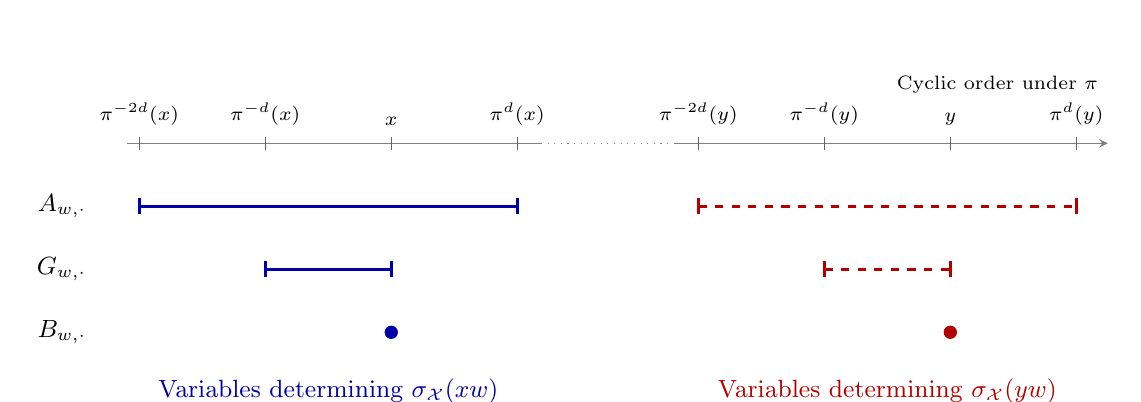
\begin{tikzpicture}[x=1cm,y=1cm,font=\small,>=stealth,
 first/.style={blue!65!black,very thick},
 second/.style={red!70!black,very thick,dashed},
 dot/.style={circle,fill,inner sep=1.7pt}]
\draw[black!50] (1.05,2.1)--(6.3,2.1);
\draw[black!50,dotted] (6.3,2.1)--(8,2.1);
\draw[->,black!50] (8,2.1)--(13.5,2.1);
\node[anchor=east,font=\scriptsize] at (13.5,2.85) {Cyclic order under $\pi$};
\foreach \p/\lab in {1.2/{\pi^{-2d}(x)},2.8/{\pi^{-d}(x)},4.4/{x},6/{\pi^d(x)},8.3/{\pi^{-2d}(y)},9.9/{\pi^{-d}(y)},11.5/{y},13.1/{\pi^d(y)}} {
 \draw[black!60] (\p,2.02)--(\p,2.18);
 \node[font=\scriptsize,above=3pt] at (\p,2.1) {$\lab$};
}
\node[anchor=east] at (.65,1.3) {$A_{w,\cdot}$};
\node[anchor=east] at (.65,.5) {$G_{w,\cdot}$};
\node[anchor=east] at (.65,-.3) {$B_{w,\cdot}$};
\draw[first] (1.2,1.3)--(6,1.3);
\draw[second] (8.3,1.3)--(13.1,1.3);
\draw[first] (2.8,.5)--(4.4,.5);
\draw[second] (9.9,.5)--(11.5,.5);
\foreach \p/\h in {1.2/1.3,6/1.3,2.8/.5,4.4/.5} {
 \draw[first] (\p,\h-.1)--(\p,\h+.1);
}
\foreach \p/\h in {8.3/1.3,13.1/1.3,9.9/.5,11.5/.5} {
 \draw[red!70!black,very thick] (\p,\h-.1)--(\p,\h+.1);
}
\node[dot,blue!65!black] at (4.4,-.3) {};
\node[dot,red!70!black] at (11.5,-.3) {};
\node[blue!65!black] at (3.6,-1.05) {Variables determining $\sigma_{\mathcal X}(xw)$};
\node[red!70!black] at (10.7,-1.05) {Variables determining $\sigma_{\mathcal X}(yw)$};
\end{tikzpicture}
\caption{Dependence ranges for two spoke states at a fixed hub $w$,
shown along one $\pi$-cycle. If $\operatorname{dist}_\pi(x,y)>3d$,
the corresponding collections of random variables are disjoint.}
\label{fig:interval:dependence-ranges}
\end{figure}



For each $w,a$, let $\xi_{w,a}$ be the vector comprising the independent
activation $A_{w,a}$, start color $G_{w,a}$ and label color $B_{w,a}$.
For fixed $w$, the variable $\sigma_{\mathcal X}(xw)$ is determined by
$(\xi_{w,\pi^k(x)})_{-2d\le k\le d}$, at most $3d+1$ vectors.
Changing $\xi_{w,a}$ can affect only $\sigma_{\mathcal X}(xw)$ with
$x\in\{\pi^k(a):-d\le k\le2d\}$, at most $3d+1$ assignments.


\section{Signed corrections in bipartite graphs}

The next lemma expresses an edge weighting with zero sum at every
vertex as a sum of alternating weightings on four-cycles. Its bound
on the total absolute coefficient at each edge will control the
change to individual wheel weights in
Theorem~\ref{thm:weights:marked-numerical}.

\begin{lemma}
\label{lem:four:sparse-alternating}
Let $0<p_*\le1$. There are $\delta_0,C>0$, depending only on $p_*$,
with the following property. Let $H$ be bipartite with parts $A,B$
of positive sizes $a,b$, let $p\in[p_*,1]$, $\delta\ge0$, and let
$D\ge1$ be an integer. Suppose that
\begin{enumerate}[label=\textup{(\roman*)}]
\item $d_H(u)=(p\pm\delta)a$ for every $u\in B$;
\item for $k\in\{2,3\}$ and distinct $u_1,\ldots,u_k\in B$,
$\left|\bigcap_{i=1}^kN_H(u_i)\right|=(p^k\pm\delta)a$; \item for every $x\in A$, there is $E_x\subseteq A$,
$|E_x|\le D$,
such that $|N_H(x)\cap N_H(y)|=p^2b\pm \delta p^2b$ for all $y\in A\setminus E_x$. \end{enumerate}
Assume $\delta+D/a+1/b\le\delta_0$. Let
\begin{equation*}
 \mathcal Q_4(H):=
 \{(x,u,y,v):x\ne y\in A,\ u\ne v\in B,\ xu,yu,yv,xv\in E(H)\},
\end{equation*}
and, for $Q=(x,u,y,v)$, let
$\delta_Q:=\ind_{xu}-\ind_{yu}+\ind_{yv}-\ind_{xv}\in\mathbb R^{E(H)}$.
For every $z:E(H)\to\mathbb R$ with
$\sum_{e\ni v}z(e)=0$ for all $v\in A\cup B$, there is
$t:\mathcal Q_4(H)\to\mathbb R$ such that
\begin{equation*}
 z=\sum_{Q\in\mathcal Q_4(H)}t(Q)\delta_Q,\qquad
 \sum_{\substack{Q\in\mathcal Q_4(H)\\Q\ni e}}|t(Q)|
 \le C\|z\|_\infty\quad(e\in E(H)).
\end{equation*}
\end{lemma}
\begin{proof}
We extend $z$ by zero to $(A\times B)\setminus E(H)$ and put
$H_{xu}:=\ind_{\{xu\in E(H)\}}$ for $x\in A$, $u\in B$.
Let $\epsilon:=\delta+D/a+1/b$.
Every constant $C_i$ below depends only on $p_*$.
Define
\begin{equation}
 Tz:=\frac1{abp^3}
 \sum_{\substack{x,y\in A\\u,v\in B}}
 H_{xu}H_{yu}H_{yv}H_{xv}z(xu)
 (\ind_{xu}-\ind_{yu}+\ind_{yv}-\ind_{xv}).
 \label{eq:sparse-alternating:S1}
\end{equation}
Terms with $x=y$ or $u=v$ have zero vector contribution. Hence
$Tz=\sum_{Q\in\mathcal Q_4(H)}t_z(Q)\delta_Q$, where
$t_z(x,u,y,v):=z(xu)/(abp^3)$. In particular,
$\sum_{v\in B}(Tz)(xv)=\sum_{y\in A}(Tz)(yu)=0$
for every $x\in A$ and $u\in B$.
A fixed edge has four possible positions in $Q$, with at most
$ab$ choices in each position. Thus
$\sum_{Q\ni e}|t_z(Q)|\le4p_*^{-3}\|z\|_\infty$ for every $e\in E(H)$.

It remains to show that repeated applications of $I-T$ converge
to zero on weightings with zero sum at every vertex.
We obtain this from a contraction bound for $(I-T)^2$.

Write $c_A(x,y):=|N_H(x)\cap N_H(y)|$ and
$c_B(u,v):=|N_H(u)\cap N_H(v)|$. Fix $xu\in E(H)$ and collect the contributions to $(Tz)(xu)$
from its four positions in an ordered four-cycle. For the first
position, (i), (iii), and $c_A(x,y)\le b$ for $y\in E_x$ give
\begin{equation*}
 \left|\frac{z(xu)}{abp^3}\sum_{y\in N_H(u)}c_A(x,y)-z(xu)\right|
 \le C_1\epsilon|z(xu)|.
\end{equation*}
The contribution from the second position is $-\frac1{abp^3}\sum_yz(yu)c_A(x,y)$. Replacing $c_A(x,y)$ by $p^2b$ gives zero since $\sum_yz(yu)=0$.
The total error is at most $C_2\epsilon\|z\|_\infty$.
The contribution from the fourth position is $-\frac1{abp^3}\sum_vz(xv)c_B(u,v)$. We replace the off-diagonal intersections by $p^2a$ and bound the
diagonal separately. The zero row sum gives an error at most
$C_3\epsilon\|z\|_\infty$.

The contribution from the third position defines the operator
\begin{equation*}
 (Kz)(xu):=\frac{H_{xu}}{abp^3}
             \sum_{y\in A,v\in B}H_{xv}H_{yu}z(yv).
\end{equation*}
This formula defines a linear operator
$K:\mathbb R^{A\times B}\to\mathbb R^{A\times B}$.
For every $z\in\mathbb R^{A\times B}$, the function $Kz$ is supported on
$E(H)$, and $\|K\|_{\infty\to\infty}\le p_*^{-3}$. On the space
\begin{equation*}
 \mathcal Z_H:=\{z\in\mathbb R^{A\times B}:
 z(xu)=0\text{ for }xu\notin E(H),\
 \sum_{u\in B}z(xu)=0\ (x\in A),\
 \sum_{x\in A}z(xu)=0\ (u\in B)\},
\end{equation*}
we have
\begin{equation}
 Tz=z+Kz+Lz,\qquad
 \|Lz\|_\infty\le C_4\epsilon\|z\|_\infty.
 \label{eq:sparse-alternating:S3}
\end{equation}
Direct substitution gives
\begin{equation}
 (K^2z)(xu)=\frac{H_{xu}}{a^2b^2p^6}
                  \sum_{s\in A,t\in B}z(st)F(x,u;s,t),
 \label{eq:sparse-alternating:S4}
\end{equation}
where
\begin{equation*}
 F(x,u;s,t):=\sum_{v\in B}H_{xv}H_{sv}
                   |N_H(u)\cap N_H(v)\cap N_H(t)|.
\end{equation*}
When $t\ne u$, the contribution to $F(x,u;s,t)$ from $v\in\{u,t\}$
is at most $2a$. Applying (ii) to the remaining terms gives $F(x,u;s,t)=ap^3c_A(x,s)\pm C_5(\delta ab+a)$. If also $s\notin E_x$, (iii)
yields $F(x,u;s,t)=abp^5\pm C_6(\delta+1/b)ab$. For all $s,t$, we have $|F(x,u;s,t)|\le ab$.
Replacing every $F$ in \eqref{eq:sparse-alternating:S4} by $abp^5$
gives zero since $\sum_{s,t}z(st)=0$.
At most $Db+a$ pairs have $s\in E_x$ or $t=u$. Consequently
\begin{equation}
 \|K^2z\|_\infty\le C_7\epsilon\|z\|_\infty.
 \label{eq:sparse-alternating:S5}
\end{equation}
Put $E:=I-T$. Since $T(\mathcal Z_H)\subseteq\mathcal Z_H$, also $E(\mathcal Z_H)\subseteq\mathcal Z_H$.
Equations \eqref{eq:sparse-alternating:S3}--\eqref{eq:sparse-alternating:S5}
give $\|Ez\|_\infty\le C_8\|z\|_\infty$ and
\begin{equation*}
 E^2z=K^2z+KLz-L(Ez),\qquad
 \|E^2z\|_\infty\le C_9\epsilon\|z\|_\infty.
\end{equation*}
Here, \eqref{eq:sparse-alternating:S3} is applied to $z,Ez\in\mathcal Z_H$.
The calculation does not require $Kz\in\mathcal Z_H$.
We choose $\delta_0$ with $C_9\delta_0\le1/2$.
For $j\ge0$, put $z_j:=(I+E)(E^2)^jz\in\mathcal Z_H$.
Then $\|z_j\|_\infty\le(1+C_8)2^{-j}\|z\|_\infty$.
Since $T(I+E)=I-E^2$, we have
$\sum_{j=0}^N Tz_j=z-(E^2)^{N+1}z\to z$.
For $Q\in\mathcal Q_4(H)$, define
$t(Q):=\sum_{j\ge0}t_{z_j}(Q)$.
The coefficient bound following \eqref{eq:sparse-alternating:S1} gives
\begin{equation*}
 \sum_{Q\ni e}|t(Q)|
 \le4p_*^{-3}\sum_{j\ge0}\|z_j\|_\infty
 \le8p_*^{-3}(1+C_8)\|z\|_\infty.
\end{equation*}
These series converge absolutely. As $\mathcal Q_4(H)$ is finite,
$\sum_Qt(Q)\delta_Q=\sum_{j\ge0}Tz_j=z$, proving the lemma
with $C=8p_*^{-3}(1+C_8)$.
\end{proof}

\section{Completion samples with prescribed hubs}

A class containing $m$ prescribed factors is assigned a $2m$-regular
spanning subgraph of a dense graph $P$. The graph $P$ itself need not
have degree $2m$. We therefore define completion samples for $P$ and
a prescribed hub set $U$ without requiring $P$ to be $2|U|$-regular.
The local estimates for these samples are used in
Propositions~\ref{prop:completion:ordinary-construction}
and~\ref{prop:completion:marked-construction}.

Let $V,U$ be finite disjoint sets, let $P$ be a simple graph on $V$,
let $\pi$ be a permutation of $V$, and let $d\ge2$ be an integer.
We use the permutation distance $\operatorname{dist}_\pi$
(Definition~\ref{def:new:permutation-intervals}).
Let $F_{\pi,3d}$ join distinct vertices at $\pi$-distance at most
$3d$. The wheel candidates used for completion have
$(3d,\pi)$-separated rim vertices.

\subsection{Ordinary completion hosts and samples}

\begin{definition}[Ordinary completion host]\label{gls:ordinary-completion-host}
\label{def:completion:ordinary-host}
The eligible ordinary edges are
\begin{equation*}
\mathfrak E^{\rm ord}
 :=\{\{x,y\}\in E(P):\operatorname{dist}_\pi(x,y)>3d\}
       \mathbin{\dot\cup}\{\{v,u\}:v\in V,\ u\in U\}.
\end{equation*}
An \emph{ordinary completion host} is $\mathcal Q=(V,U,R,H)$,
where $R$ is a graph on $V$, $H$ is bipartite on $V,U$, and
$E(R)\mathbin{\dot\cup}E(H)\subseteq\mathfrak E^{\rm ord}$.
\end{definition}

For\phantomsection\label{gls:restricted-balance-differences} an integer $r\ge3$ and an ordinary completion host $\mathcal Q$,
we write $\mathcal W(\mathcal Q):=\mathcal W_r^{\rm ord}(\mathcal Q)$.
For $A\subseteq V$, $B\subseteq U$ and every $v\in V$, let
\begin{equation}
 b(v):=d_R(v)-2d_H(v),\qquad
 b^{A,B}(v):=d_R(v;A)-2d_H(v;B).
\end{equation}
These functions are defined also when $v\notin A$.
The host is \emph{$r$-wheel-divisible} when $b(v)=0$ for every
$v\in V$ and $r\mid d_H(u)$ for every $u\in U$.
Deleting edge-disjoint ordinary $r$-wheels from $\mathcal Q$ leaves
$b(v)$ unchanged for every $v\in V$ and changes each $d_H(u)$ by a
multiple of $r$. Hence $r$-wheel-divisibility is preserved.

\begin{definition}[Ordinary completion sample]\label{gls:ordinary-completion-sample}
\label{def:ordinary-local-reference}
Let $P$ be a graph on $V$, let $U$ be disjoint from $V$, let $d\ge2$ be an integer,
and let $\pi$ be a permutation of $V$ with $L_\pi>10d$.
Let $0<\varrho\le1$, $0<s\le1/100$ and $a_u,b_u\ge0$ satisfy
\begin{equation}
 a_u\le1/8,\qquad
 s+b_u\le\overline q(u):=1-(1+1/d)a_u\quad(u\in U).
 \label{eq:completion:ordinary-pair-feasibility}
\end{equation}
Let $(\mathcal X_u^g)$ and $(B_{u,x})$ be the interval families and label variables of a raw interval sample with interval color $2$ and label
colors $\mathrm o_1,\mathrm o_2$, using the functions
$q_2(u):=a_u$, $s_{\mathrm o_1}(u):=s$ and
$s_{\mathrm o_2}(u):=b_u$. Let $H_{\rm ord}$ be the bipartite graph on $(V,U)$ with
\begin{equation*}
 E(H_{\rm ord}):=\{xu:\sigma_{\mathcal X}(xu)=\mathrm o_1\}
       =\{xu:x\in\overline X_u,\ B_{u,x}=\mathrm o_1\}.
\end{equation*}
Let $R$ be obtained by sampling the edges of $P$ independently with
probability $\varrho s$, independently of $(A_{u,a}),(G_{u,a}),(B_{u,x})$,
and retaining precisely those sampled edges $xy$ with $\operatorname{dist}_\pi(x,y)>3d$.
We call $\mathcal B:=(R,H_{\rm ord})$ the \emph{ordinary completion sample}
with parameters $\varrho,s,d,(a_u),(b_u)$. Neither $R$ nor $H_{\rm ord}$ has edge types.
\end{definition}

\subsection{Marked completion hosts and samples}

\begin{definition}[Marked completion host]\label{gls:marked-completion-host}
\label{def:completion:marked-host}
Here, $\pi$ is a permutation of $V$. The eligible occurrences for marked-wheel completion are
\begin{equation*}
\begin{split}
 \mathfrak E^{\rm mark}
 &:=\{(x,y,j):x,y\in V,\ j\in\{0,K\},\
       \operatorname{dist}_\pi(x,y)>3d,\ \operatorname{phys}(x,y,j)\in E(P)\}\\
 &\qquad\mathbin{\dot\cup}\{(v,u,j):v\in V,\ u\in U,\ j\in\{0,K\}\}.
\end{split}
\end{equation*}
Here, $\operatorname{phys}(x,y,0)=\{x,y\}$ and
$\operatorname{phys}(x,y,K)=\{x,\pi(y)\}$.
For $A\subseteq V$ and $B\subseteq U$, let
\begin{equation*}
 \mathfrak E^{\rm mark}(A,B)
 :=\mathfrak E^{\rm mark}\cap
 ((A\times A\times\{0,K\})\dot\cup(A\times B\times\{0,K\})).
\end{equation*}

A \emph{marked completion host} is a tuple
$\mathcal Q=(V,U,R^0,R^K,H^0,H^K)$, where $R^0,R^K$ are digraphs
on $V$ and $H^0,H^K$ are bipartite on $V,U$, satisfying
\begin{equation*}
 (x,y,j)\in\mathfrak E^{\rm mark}\quad(x\to y\in E(R^j)),\qquad
 (v,u,j)\in\mathfrak E^{\rm mark}\quad(vu\in E(H^j))
 \quad(j\in\{0,K\}).
\end{equation*}
Moreover,
$E(H^0)\cap E(H^K)=\varnothing$ and
\begin{equation}
 N_{H^0}(u)\cap\pi(N_{H^K}(u))=\varnothing\quad(u\in U).
 \label{eq:completion:successor-disjointness}
\end{equation}
Let $R:=R^0\dot\cup R^K$ and $H:=H^0\dot\cup H^K$, retaining types.

\end{definition}

For\phantomsection\label{gls:restricted-balance-differences:marked} an even integer $c\ge8$ and a marked completion host $\mathcal Q$,
we write $\mathcal W(\mathcal Q):=\mathcal W_c^K(\mathcal Q)$.
For $A\subseteq V$, $B\subseteq U$, $v\in V$ and $u\in U$, let
\begin{equation}
\begin{aligned}
 a^{+,A,B}(v)&:=d_R^+(v;A)-d_H(v;B),&
 a^{-,A,B}(v)&:=d_R^-(v;A)-d_H(v;B),\\
 a^{K,A,B}(v)&:=d_{R^K}^-(v;A)-d_{H^K}(v;B),&
 a^{U,A}(u)&:=d_{H^0}(u;A)-(c-1)d_{H^K}(u;A).
\end{aligned}
\label{eq:completion:marked-differences}
\end{equation}
The four restricted functions in~\eqref{eq:completion:marked-differences}
are evaluated for every $v\in V$ and $u\in U$, including vertices outside
$A$ and hubs outside $B$. We write $a^+:=a^{+,V,U}$, $a^-:=a^{-,V,U}$,
$a^K:=a^{K,V,U}$ and $a^U:=a^{U,V}$.
A\phantomsection\label{gls:marked-wheel-divisibility} host is \emph{marked $c$-wheel-divisible} when
$a^+=a^-=a^K=a^U=0$. For a marked wheel $W=W(C,u)$ with
auxiliary rim $C=(v_0,\ldots,v_{c-1},v_0)$ and marked arc
$v_{c-1}\to v_0$, its rim and spoke graphs satisfy, for $v\in V$ and $u'\in U$,
\begin{equation*}
\begin{aligned}
 d_{R_W}^+(v)=d_{R_W}^-(v)=d_{H_W}(v)
    &=\ind_{\{v\in V(C)\}},\\
 d_{R_W^K}^-(v)=d_{H_W^K}(v)&=\ind_{\{v=v_0\}},\\
 d_{H_W^0}(u')=(c-1)d_{H_W^K}(u')
    &=(c-1)\ind_{\{u'=u\}}.
\end{aligned}
\end{equation*}
Consequently deleting $W$ preserves the four full differences
$a^+,a^-,a^K,a^U$. The same holds for an edge-disjoint family
of marked wheels, and hence preserves marked $c$-wheel-divisibility.

For the interval sample below, we recall that
$I_a=\{\pi^t(a):0\le t<d\}$ and $I_a^+=\pi^d(a)$.

\begin{definition}[Marked completion sample]\label{gls:marked-completion-sample}
\label{def:completion:marked-sample}
Let $P$ be a graph on $V$, let $U$ be disjoint from $V$, let $d\ge2$ be an integer,
and let $\pi$ be a permutation of $V$ with $L_\pi>10d$.
Let $c\ge8$ be even, $0<\varrho\le1$, $0<s\le1/100$, and let
\begin{equation}
 t:=\frac{s}{c-1},\qquad p:=\frac{\varrho s}{2},\qquad
 k:=\frac{\varrho t}{2}.
 \label{eq:family:marked-probabilities}
\end{equation}
Let $a_u,b_u\ge0$ satisfy
\begin{equation}
 t+a_u\le1/8,\qquad
 s+b_u\le\overline q(u):=1-(1+1/d)(t+a_u)\quad(u\in U).
 \label{eq:completion:pair-feasibility}
\end{equation}
Let $(\mathcal X_u^g)$ and $(B_{u,x})$ be the interval families and label variables of a raw interval sample with interval colors $1,2$ and label
colors $\mathrm o_1,\mathrm o_2$, using the functions
$q_1(u):=t$, $q_2(u):=a_u$,
$s_{\mathrm o_1}(u):=s$, $s_{\mathrm o_2}(u):=b_u$. Define the spoke graphs by
\begin{equation*}
 E(H^0):=\{xu:\sigma_{\mathcal X}(xu)=\mathrm o_1\},\qquad
 E(H^K):=\{xu:\sigma_{\mathcal X}(xu)=1\}.
\end{equation*}

Let $(C_e)_{e\in E(P)}$ be independent random variables, independent of
the raw interval and label variables.
For $e=\{x,y\}$, each of the states $(x,y,0)$ and $(y,x,0)$ has
probability $p$, and each of $(x,y,K)$ and $(y,x,K)$ has probability $k$.
The remaining probability is assigned to $\bot$.
Here, $C_e=(x,y,j)$ records the direction $x\to y$ of the physical edge
$e$ and its type $j$. The corresponding auxiliary arc is $(x\to y,0)$
when $j=0$ and $(x\to\pi^{-1}(y),K)$ when $j=K$. Thus
\begin{equation*}
\begin{aligned}
 E(R^0)&:=\{x\to y:xy\in E(P),\ C_{xy}=(x,y,0),\
                         \operatorname{dist}_\pi(x,y)>3d\},\\
 E(R^K)&:=\{x\to z:x\pi(z)\in E(P),\ C_{x\pi(z)}=(x,\pi(z),K),\
                         \operatorname{dist}_\pi(x,z)>3d\}.
\end{aligned}
\end{equation*}
We call $\mathcal B:=(R^0,R^K,H^0,H^K)$ the
\emph{marked completion sample} with parameters
$c,\varrho,s,d,(a_u),(b_u)$.
\end{definition}

\subsection{Auxiliary and physical degrees}
\label{subsec:pr:representations}

Throughout this subsection, $V^{\rm amb}$ and $U$ are disjoint finite sets,
$V\subseteq V^{\rm amb}$, and $\pi$ is a permutation of $V^{\rm amb}$.
For\phantomsection\label{gls:auxiliary-and-physical-incidence-degrees} a multiset $D$ of typed arcs on $V$ and typed spokes between $V,U$,
let $d_{\rm aux}(z;D)$ count incidences at $z$ at the auxiliary
endpoints, and let $d_{\rm phys}(z;D)$ count incidences at their
physical images. Both count multiplicities and both ends of a loop.
Both functions are defined on $V^{\rm amb}\cup U$. Moreover,
$d_{\rm aux}(z;D)=0$ for every $z\in V^{\rm amb}\setminus V$.
With maxima over $z\in V^{\rm amb}\cup U$, let
\begin{equation*}
 \Delta_{\rm aux}(D):=\max_z d_{\rm aux}(z;D),\qquad
 \Delta_{\rm phys}(D):=\max_z d_{\rm phys}(z;D),\qquad
 \Delta_*(D):=\max\{\Delta_{\rm aux}(D),\Delta_{\rm phys}(D)\}.
\end{equation*}
For every $v\in V^{\rm amb}$,
\begin{equation}
 d_{\rm aux}(v;D)\le d_{\rm phys}(v;D)+d_{\rm phys}(\pi(v);D),
 \qquad
 d_{\rm phys}(v;D)\le d_{\rm aux}(v;D)+d_{\rm aux}(\pi^{-1}(v);D).
 \label{eq:physical:degree-comparison}
\end{equation}
For a marked arc, the auxiliary head $v$ corresponds to the physical
head $\pi(v)$, and a physical head $v$ corresponds to the auxiliary
head $\pi^{-1}(v)$. Type-$0$ arcs and spokes of either type retain their endpoints.
For $u\in U$, the two incidence counts agree. Consequently,
$\Delta_*(D)\le2\Delta_{\rm phys}(D)$ and
$\Delta_*(D)\le2\Delta_{\rm aux}(D)$.

For\phantomsection\label{gls:auxiliary-and-physical-incidence-degrees:difference} typed extended graphs $\mathcal Q=(R^0,R^K,H^0,H^K)$ and
$\widetilde{\mathcal Q}=(\widetilde R^0,\widetilde R^K,
\widetilde H^0,\widetilde H^K)$ on the same $(V,U,\pi)$,
with the same ambient set $V^{\rm amb}$, arc occurrences are indexed
in a common finite set, with a fixed tail, head and type for each
index. Symmetric differences are taken between these sets of occurrences. Let
\begin{equation*}
 D:=(E(R^0)\triangle E(\widetilde R^0))\dot\cup
 (E(R^K)\triangle E(\widetilde R^K))\dot\cup
 (E(H^0)\triangle E(\widetilde H^0))\dot\cup
 (E(H^K)\triangle E(\widetilde H^K)).
\end{equation*}
This union retains types and directions. Deleting an arc and
inserting another type or direction counts twice.
For ordinary extended graphs $(V,U,R,H)$ and
$(V,U,\widetilde R,\widetilde H)$, let
$D:=(E(R)\triangle E(\widetilde R))\dot\cup
(E(H)\triangle E(\widetilde H))$. The two incidence counts agree.

If the typed extended graph $\mathcal Q$ is physically injective, let
$R:=R^0\dot\cup R^K$, $H:=H^0\dot\cup H^K$.
For a graph $F$ with $E(F)\subseteq E_{\rm phys}(\mathcal Q)$, let
$D_F:=\{e\in E(R)\dot\cup E(H):\operatorname{phys}(e)\in E(F)\}$,
retaining the typed edge and arc occurrences. Then $\Delta_*(D_F)\le2\Delta(F)$. Physical injectivity gives
$\Delta_{\rm phys}(D_F)\le\Delta(F)$,
so \eqref{eq:physical:degree-comparison} applies. If $R^K$ is empty,
the two incidence counts agree and $\Delta_*(D_F)\le\Delta(F)$.

\subsection{Restrictions and edge changes in completion hosts}

For a completion host $\mathcal Q$ and $A\subseteq V$, $B\subseteq U$,
the induced extended subgraph $\mathcal Q[A\cup B]$ has parts $A,B$ and
consists of the edges or arcs of $R$ with both auxiliary endpoints in $A$
and the edges of $H$ between $A$ and $B$. In the marked case, it retains
the directions, types and physical images computed with the ambient
permutation $\pi$. We use $\pi|_A$ only when $\pi(A)=A$.

Let\phantomsection\label{gls:star-of-a-vertex-hub-pair} $\mathfrak E$ denote $\mathfrak E^{\rm ord}$ or
$\mathfrak E^{\rm mark}$ according to the model. For an ordinary
edge $e$, let $a_1(e),a_2(e)$ be its endpoints in either order.
For a typed rim arc $e=(x,y,j)$ let $(a_1(e),a_2(e)):=(x,y)$;
for a typed spoke $e=(v,u,j)$ let $(a_1(e),a_2(e)):=(v,u)$.
We define
\begin{equation*}
\operatorname{star}(A,B):=\{e\in\mathfrak E:
       \{a_1(e),a_2(e)\}\cap(A\cup B)\ne\varnothing\}.
\end{equation*}
Thus the star includes crossing edges and all potential occurrences
with an endpoint in $A\cup B$, whether or not they are present.
If $\pi(A)=A$, the same set is obtained using physical endpoints.
Let $d_{\rm aux},d_{\rm phys}$ and $\Delta_*$ be the incidence degrees
and maximum degree defined in Section~\ref{subsec:pr:representations}. They are applied to
the typed symmetric difference when comparing hosts: changing a
direction or type counts both the removed and the inserted typed occurrence.

For $\pi$-invariant $A\subseteq V$ and $B\subseteq U$, the spoke
assignments on $A\times B$ are restrictions of the original assignments,
using the original activation, start-color and label-color variables.
For every $v\in V$ and $u\in U$, the ordinary sample satisfies
$\Pr(vu\in E(H_{\rm ord}))=s$, while the marked sample satisfies
$\Pr(vu\in E(H^0))=s$ and $\Pr(vu\in E(H^K))=t$.

For $M:=|U|$ and $D_0:=2M/\varrho$, the sampling probabilities satisfy
$(\varrho s)D_0=2Ms$, $pD_0=Ms$ and $kD_0=Mt$.
The inequalities in~\eqref{eq:completion:pair-feasibility} also give $\overline q(u)\ge13/16$ and
$2p+2k=\varrho(s+t)\le1$, so all probabilities above are valid.


For $\varrho\in[\varrho_*,1]$ and $s\in[s_*,1/100]$, the probabilities
used in the denominators of the cycle and wheel weights satisfy
\begin{equation*}
\begin{gathered}
 \varrho s\ge\varrho_*s_*,\quad s\ge s_*,\quad
 p\ge\varrho_*s_*/2,\quad k\ge\varrho_*s_*/(2(c-1)),\\
 t\ge s_*/(c-1),\qquad s^2/(c-1)\ge s_*^2/(c-1).
\end{gathered}
\end{equation*}
These denominators contain neither $a_u,b_u$ nor
$\Pr(\sigma_{\mathcal X}(vu)=\bot)$, which may be zero.
The ordinary and marked sampling estimates in
Lemmas~\ref{lem:completion:ordinary-reference},
\ref{lem:completion:marked-reference} and
Section~\ref{subsec:completion:marked-sampling} use these lower bounds.
Their conclusions hold for each fixed choice of the arrays $(a_u,b_u)$
satisfying \eqref{eq:completion:ordinary-pair-feasibility} or
\eqref{eq:completion:pair-feasibility}, with constants uniform over those arrays.
Excluding labels at $\pi$-distance at most $3d$ from a bounded number
of fixed labels removes $O_{r,c}(d)$ vertices. The required order
thresholds and the concentration constants may therefore depend on $d$.
The raw pair assignments in Lemma~\ref{lem:interval:raw-law} are
independent of the Bernoulli rim-edge choices in the ordinary sample
and of $(C_e)_{e\in E(P)}$ in the marked sample.
Fix $u\in U$ and $T\subseteq V$ with $|T|=h$, without requiring separation
between the vertices of $T$. Let
$A_0:=\bigcup_{x\in T}\{\pi^{-j}(x):0\le j\le d\}$.
If $A_{u,a}=0$ for every $a\in A_0$ and $B_{u,x}=\mathrm o_1$
for every $x\in T$, then $\sigma_{\mathcal X}(xu)=\mathrm o_1$ for all $x\in T$.
Since $|A_0|\le h(d+1)$ and these variables are independent,
\begin{equation*}
 \Pr\bigl(\sigma_{\mathcal X}(xu)=\mathrm o_1\text{ for all }x\in T\bigr)
 \ge\left(1-\frac1{2d+1}\right)^{h(d+1)}s_*^h
 \ge e^{-3h/2}s_*^h.
\end{equation*}
For disjoint sets $T_0,T_K$ whose union is $(3d,\pi)$-separated,
Lemma~\ref{lem:interval:raw-law} gives, in the marked completion sample,
\begin{equation*}
 \Pr\bigl(\sigma_{\mathcal X}(xu)=\mathrm o_1\ (x\in T_0),\
           \sigma_{\mathcal X}(xu)=1\ (x\in T_K)\bigr)
 =s^{|T_0|}t^{|T_K|}.
\end{equation*}
These two spoke-presence probability estimates are uniform over
the feasible arrays $(a_u,b_u)$ and in $d$.

In applications with $\delta(P)\ge(1/2+\alpha)|V|$,
$\varrho\in[\varrho_*,1]$ and $s\in[s_*,1/100]$, we set
$p_{\rm rim}:=\varrho_*s_*/2$ and choose an even
$c\ge\max\{8,c_0(\alpha/4,p_{\rm rim}),c_{\rm succ}(\alpha/4)\}$.
Here $c_0$ is the cutoff in Theorem~\ref{thm:capacity:marked-numerical}
and $c_{\rm succ}$ is the cutoff in
Theorem~\ref{thm:four:successor-kernel}.
The former applies uniformly for $p=\varrho s/2\ge p_{\rm rim}$,
and the latter supplies the initial positional weights.
This choice precedes the interval length and all approximation errors.


\section{Weighted subgraph estimates}

We first bound the change in weighted subgraph counts when edges are
altered, and prove concentration estimates for these counts under
independent sampling. The last lemma bounds the total weight of candidate
wheels containing two distinct physical edges, each of which may be a
rim edge or a spoke.


Let\phantomsection\label{gls:weighted-candidate-count-with-omitted-root-subgraph} $\mathcal C$ be a finite indexed family
of candidate subgraphs of an ordinary or typed extended graph,
with all directions and assigned edge types fixed. Their physical edge sets are those of
Definition~\ref{def:ephys}. In the union of several constituent cycles, a shared physical edge is
included once. Candidates that assign incompatible types or directions
to it are excluded.
Let $(w_C)_{C\in\mathcal C}$ be fixed nonnegative coefficients
and let $F_0$ be a fixed subgraph contained in every candidate.
We count candidates whose edges outside $F_0$ belong to $\mathcal Q$,
without requiring $F_0\subseteq\mathcal Q$, by
\begin{equation*}
L_{F_0}(\mathcal Q):=\sum_{C\in\mathcal C}w_C
             \ind_{\{C-E(F_0)\subseteq\mathcal Q\}}.
\end{equation*}
Inclusion respects all displayed types and directions.
When $F_0\subseteq\mathcal Q$, it equals
$\sum_{C\in\mathcal C:\,C\subseteq\mathcal Q}w_C$.
Any normalization is incorporated into the fixed coefficients $w_C$.

For a random sample $\mathcal B$,
$\mathbb E L_{F_0}(\mathcal B) =\sum_{C\in\mathcal C}w_C \Pr(C-E(F_0)\subseteq\mathcal B)$. The probability is
taken in the original sampling experiment,
without conditioning on the presence of $F_0$. The later applications
compute these probabilities from the independent variables defining
the sample.


\begin{lemma}
\label{lem:pr:weighted-count-change}
Let $\mathcal Q,\mathcal Q'$ be ordinary extended graphs on the same
sets $V,U$, or typed extended graphs on $(V,U,\pi)$ with the same
ambient set $V^{\rm amb}$ and permutation $\pi$.
Let $a>0$, $B_Z\ge0$, and let $f,J\ge1$ and $q\ge0$ be integers.
Let $S\subseteq V\cup U$, let $X:=\{x_1,\ldots,x_f\}$ be disjoint
from $V\cup U$, and let $T$ be a simple graph on $S\cup X$ with
$E(T[S])=\varnothing$ and $|E(T)|\le q$.
For a finite index set $\mathcal I$, let
$\varphi_\alpha:S\cup X\to V\cup U$, $\alpha\in\mathcal I$, be maps
satisfying $\varphi_\alpha(s)=s$ for every $s\in S$ and
$\varphi_\alpha(x_j)\in A_j$ for $1\le j\le f$,
where $|A_j|\le2a$ and $\left|\bigcup_{j=1}^f A_j\right|\le3a$.
Each
tuple $(v_1,\ldots,v_f)$ occurs as
$(\varphi_\alpha(x_1),\ldots,\varphi_\alpha(x_f))$
for at most $J$ indices $\alpha$.

For each $\alpha$, let $F_\alpha$ be a fixed set of edges or typed arcs and
spokes, and let $0\le w_\alpha\le B_Za^{-f}$ be a fixed coefficient.
Writing $\partial e$ for the unordered pair of auxiliary endpoints
of $e$, assume
\begin{equation*}
 \partial e\in
 \bigl\{\{\varphi_\alpha(x),\varphi_\alpha(y)\}:xy\in E(T)\bigr\}
 \quad(e\in F_\alpha).
\end{equation*}
Let
\begin{equation*}
 Z(\mathcal R):=\sum_{\alpha\in\mathcal I}w_\alpha
       \prod_{e\in F_\alpha}\ind_{\{e\in E(\mathcal R)\}}
       \quad(\mathcal R=\mathcal Q,\mathcal Q'),\qquad
 D:=(E(\mathcal Q)\triangle E(\mathcal Q'))\cap
       \bigcup_{\alpha\in\mathcal I}F_\alpha.
\end{equation*}
If $\Delta_*(D)\le u_{\rm ch}$, then
\begin{equation}
 |Z(\mathcal Q')-Z(\mathcal Q)|
 \le K_{\rm prod}(f,q,J,B_Z)\frac{u_{\rm ch}}a,\qquad
 K_{\rm prod}(f,q,J,B_Z):=2^{f+3}JqB_Z.
 \label{eq:incidence:normalized-change}
\end{equation}
\end{lemma}
\begin{proof}
Each product in $Z$ is $0$ or $1$ and is unchanged when
$F_\alpha\cap D=\varnothing$. Hence
$|Z(\mathcal Q')-Z(\mathcal Q)|
\le\sum_{\alpha:F_\alpha\cap D\ne\varnothing}w_\alpha$.
For $xy\in E(T)$, let
\begin{equation*}
 \mathcal I_{xy}:=\{\alpha\in\mathcal I:
  \text{some }e\in F_\alpha\cap D\text{ satisfies }
  \partial e=\{\varphi_\alpha(x),\varphi_\alpha(y)\}\}.
\end{equation*}
The assumption on $\partial e$ gives
$\{\alpha:F_\alpha\cap D\ne\varnothing\}
\subseteq\bigcup_{xy\in E(T)}\mathcal I_{xy}$.
Since $E(T[S])=\varnothing$, each edge of $T$ has at least one
endpoint in $X$.

Suppose first that $x\in S$ and $y\in X$.
The equality $\varphi_\alpha(x)=x$ and the bound
$d_{\rm aux}(x;D)\le\Delta_*(D)\le u_{\rm ch}$ leave at most
$u_{\rm ch}$ possible occurrences of $D$ incident with this root.
Each occurrence determines $\varphi_\alpha(y)$, and the other
$f-1$ labels have at most $(2a)^{f-1}$ choices.
The multiplicity bound $J$ therefore gives
$|\mathcal I_{xy}|\le2Ju_{\rm ch}(2a)^{f-1}$.
If $x,y\in X$, there are at most $3au_{\rm ch}$ occurrences of $D$
with both auxiliary endpoints in $\bigcup_j A_j$.
Assigning the two endpoints to $x,y$ in either order and choosing
the other $f-2$ labels gives
$|\mathcal I_{xy}|\le6Jau_{\rm ch}(2a)^{f-2}$.
These counts include all directions, types and arc occurrences.
Multiplying by $B_Za^{-f}$ and summing over the at most $q$ edges
of $T$ proves \eqref{eq:incidence:normalized-change}.
\end{proof}



\begin{lemma}\label{lem:pr:wi-interactions}
Let $C,B\ge1$ and $a\ge1$. Let $E,J$ be finite,
let $\mathcal T$ be a finite indexed family of subsets of $E$, and
let $w_T\ge0$ for $T\in\mathcal T$. We define
\begin{equation*}
 \mathscr Z(\mathbf u):=\sum_{T\in\mathcal T}w_T\prod_{f\in T}u_f
       \quad(\mathbf u\in\{0,1\}^E),\qquad b(f):=\sum_{T\ni f}w_T.
\end{equation*}
Let independent coordinates $\xi_j\in\mathcal Z_j$, $j\in J$,
determine indicators $I_f:\prod_{j\in J}\mathcal Z_j\to\{0,1\}$,
and let $Z(\mathbf z):=\mathscr Z((I_f(\mathbf z))_{f\in E})$.
Suppose $E_1\dot\cup E_2=\{f:b(f)>0\}$ satisfies
\begin{equation*}
 |E_1|\le Ca,\quad b(f)\le C/a\ (f\in E_1),\qquad
 |E_2|\le Ca^2,\quad b(f)\le C/a^2\ (f\in E_2).
\end{equation*}
Assume each $I_f$ with $b(f)>0$ depends on at most $B$ coordinates,
and any change of one coordinate changes at most $B$ such indicators.

Then there are $c_j\ge0$, $j\in J$, such that
\begin{equation*}
 \sum_{j\in J}c_j^2\le2C^3B^3/a,\qquad
 |Z(\mathbf z)-Z(\mathbf z')|\le c_j
 \quad\text{if }z_i=z_i'\text{ for every }i\ne j.
\end{equation*}
\end{lemma}

The proof is given in Appendix~\ref{app:proof:lem-pr-wi-interactions}.




\paragraph{Cycle and successor-path incidences.}
Let\phantomsection\label{gls:candidate-wheel-indices-and-physical-incidence-sets} $P$ be a graph on $V$, let $U$ be disjoint from $V$, and let
$\pi$ be a permutation of $V$. Let
$E_V:=E(P)$, $E_{VU}:=\{\{v,u\}:v\in V,\ u\in U\}$ and
$E:=E_V\dot\cup E_{VU}$.
A candidate index is $i=(0,w,r,\mathbf x)$ with integer $r\ge3$
and $\mathbf x\in V^r$, or $i=(K,w,c,\mathbf x)$ with integer
$c\ge4$ and $\mathbf x\in V^c$. In both cases $w\in U$ and the
entries of $\mathbf x$ are distinct. Let $q_i:=r$ in the first case
and $q_i:=c$ in the second, and let $\tau_i\in\{0,K\}$ be the
first entry of $i$. Number the entries $0,\ldots,q_i-1$ and
let $x_{q_i}:=x_0$. We define
\begin{equation}
 \vec e_{i,h}:=
 \begin{cases}
 (x_{q_i-1},\pi(x_0)),&\tau_i=K,\ h=q_i-1,\\
 (x_h,x_{h+1}),&\text{otherwise},
 \end{cases}
 \qquad
 t_{i,h}:=\begin{cases}K,&\tau_i=K,\ h=q_i-1,\\0,&\text{otherwise}.
 \end{cases}
 \label{eq:mixed:ordered-physical-map}
\end{equation}
We consider only tuples for which the underlying unordered edges
$e_{i,h}$ are distinct members of $E(P)$. Let
\begin{equation}
 E_V(i):=\{e_{i,h}:0\le h<q_i\},\qquad
 E_U(i):=\{\{x_h,w\}:0\le h<q_i\},\qquad
 \iota(i):=E_V(i)\cup E_U(i).
 \label{eq:mixed:physical-incidence}
\end{equation}
The hub and ordered tuple remain part of the index even when two
indices have the same physical edge set $\iota(i)$.

\begin{lemma}
\label{lem:pr:wheel-codegrees}
Let $P$ be a graph on $V$, let $U$ be disjoint from $V$, and let
$\pi$ be a permutation of $V$. Let $n:=|V|\ge1$ and assume $|U|\le n$.
Let $\mathcal I$ be a set of candidate indices $(0,w,r,\mathbf x)$ and $(K,w,c,\mathbf x)$
with the physical maps in
\eqref{eq:mixed:ordered-physical-map}--\eqref{eq:mixed:physical-incidence}.
Each tuple has distinct entries and its rim images are distinct edges of $P$.
Suppose $q_i$ belongs to a fixed finite set $\mathcal L$ and
$0\le\Omega(i)\le A_{q_i}n^{1-q_i}$ for $i\in\mathcal I$.
There is a constant $K_{\rm cd}$, depending only on
$\mathcal L$ and $(A_q)_{q\in\mathcal L}$, such that
\begin{equation}
 \sum_{\substack{i\in\mathcal I\\ e,f\in\iota(i)}}\Omega(i)
 \le K_{\rm cd}/n
 \qquad(e,f\in E_V\dot\cup E_{VU},\ e\ne f).
 \label{eq:preparation:wheel-codegrees}
\end{equation}
\end{lemma}
\begin{proof}
Fix distinct $e,f\in E_V\dot\cup E_{VU}$, a length $q\in\mathcal L$
and a type $\tau\in\{0,K\}$. Fix also the positions of $e,f$ in
a candidate of this length and type, and an orientation for each
of them that is a rim edge.
By \eqref{eq:mixed:ordered-physical-map}, a physical rim edge
oriented from $a$ to $b$ at position $h$ determines auxiliary labels
$a,b$ when $t_{i,h}=0$, and $a,\pi^{-1}(b)$ when $t_{i,h}=K$.
Inconsistent assignments give no candidates.

If $e,f$ are rim edges, their distinct positions determine at least
three entries of the tuple. There are at most $n^{q-3}$ choices
for the remaining entries and at most $n$ choices for the hub.
If one is a rim edge and the other a spoke, they determine the hub
and at least two tuple entries, leaving at most $n^{q-2}$ candidates.
Two spokes with different hubs occur in no common candidate.
Two distinct spokes with the same hub determine that hub and two
tuple entries, again leaving at most $n^{q-2}$ candidates.
Thus, for each fixed choice of positions and orientations, the sum
of coefficients is at most
$n^{q-2}A_qn^{1-q}=A_q/n$.
Summing over the bounded number of lengths, types, positions and
orientations proves \eqref{eq:preparation:wheel-codegrees}.
\end{proof}

\section{Fractional ordinary wheel decompositions}
\label{sec:four:relative-weights}

We give a deterministic criterion for correcting an ordinary $r$-wheel
weighting so that every rim and spoke edge has load one. The proof
first corrects the rim loads using signed cycle weights on bounded
dense subgraphs, then corrects the spoke loads while preserving the
rim loads. The input weighting and configuration counts will be
supplied by sampling in later sections. Related local corrections
of fractional weights, with quantitative bounds on individual
coefficients, were developed by Barber, K\"uhn, Lo, Montgomery
and Osthus~\cite[Section~5]{BKLMO2017Fractional}.

\begin{lemma}
\label{lem:four:edge-isolator}
Let $r\ge3$ and $\alpha>0$. There exists $m_0=m_0(r,\alpha)$ such that
the following holds for every integer $m\ge m_0$.
Let $B$ be a graph on $m$ vertices with
$\delta(B)\ge(\delta_{C_r}+\alpha)m$, and let $e\in E(B)$.
Then there is $I_{B,e}:\mathcal C_r(B)\to\mathbb R$ such that
\begin{equation*}
\sum_{C\ni f}I_{B,e}(C)=\ind_{\{f=e\}}\quad(f\in E(B)),\qquad
|I_{B,e}(C)|\le1\quad(C\in\mathcal C_r(B)),
\end{equation*}
and
\begin{equation*}
\sum_{C\ni v}I_{B,e}(C)=\tfrac12\ind_{\{v\in e\}}\quad(v\in V(B)).
\end{equation*}
\end{lemma}
\begin{proof}
We choose $m_0$ so that the definition of $\delta_{C_r}^*$ applies
with margin $\alpha/2$ for every $m\ge m_0$, and
$1\le\alpha m_0/2$. These requirements hold uniformly for bounded
$r$ and a fixed positive lower bound on $\alpha$. By Theorem~\ref{thm:four:cycle-fractional-threshold}, we have $\delta_{C_r}^*\le\delta_{C_r}$.
Hence $B$ has a fractional $C_r$-decomposition $\lambda_B$.
Moreover, $\delta(B-e)\ge\delta(B)-1 \ge(\delta_{C_r}^*+\alpha)m-1 \ge(\delta_{C_r}^*+\alpha/2)m$, so $B-e$
has a fractional $C_r$-decomposition
$\lambda_{B-e}$. We extend $\lambda_{B-e}$ by zero to the
$C_r$-copies of $B$ that use $e$, and put $I_{B,e}:=\lambda_B-\lambda_{B-e}$. Subtracting the two fractional decompositions gives
$\sum_{C\ni f}I_{B,e}(C)=\ind_{\{f=e\}}$ for $f\in E(B)$.
Their coefficients lie in $[0,1]$, so $|I_{B,e}(C)|\le1$.
Finally, $2\sum_{C\ni v}I_{B,e}(C) =\sum_{f\ni v}\sum_{C\ni f}I_{B,e}(C) =\ind_{\{v\in e\}}$, which proves the vertex-sum identity.
\end{proof}

\subsection{A criterion for correcting rim and spoke loads}


Let $r\ge3$, $k\ge r+2$ and $\vartheta,\alpha>0$. Let $P,\mathcal F$
be graphs on $V$, let $U$ be disjoint from $V$, let
$Q\subseteq P^{\rm adm}:=P-E(\mathcal F)$, and let $H$ be a bipartite
graph with parts $V,U$.
Let\phantomsection\label{gls:ordinary-rim-and-spoke-load-operators} $n:=|V|$. For a signed ordinary $r$-wheel weighting $\psi$, we define
its rim and spoke load vectors by
\begin{equation*}
 (\mathcal L_R\psi)(e):=\sum_{W:e\in E(W)}\psi(W)\quad(e\in E(Q)),\qquad
 (\mathcal L_H\psi)(e):=\sum_{W:e\in E(W)}\psi(W)\quad(e\in E(H)).
\end{equation*}
We use two families of configurations.
\paragraph{Rim-load correction configurations.}
The first family supplies graphs $P[S]$ for which
Lemma~\ref{lem:four:edge-isolator} gives a signed weighting
$I_{P[S],e}$ with load $1$ at $e$ and load $0$ at every other edge of $P[S]$.
For\phantomsection\label{gls:rim-load-correction-configurations} $e=xy\in E(Q)$ and $u\in N_H(x)\cap N_H(y)$, let
$\mathcal S(e,u)$ consist of the $k$-sets $S$ with $E(\mathcal F[S])=\varnothing$ such that
\begin{equation}
 \{x,y\}\subseteq S\subseteq N_H(u),\qquad
 P[S]\subseteq Q,\qquad \delta(P[S])\ge(\vartheta+\alpha/4)k.
\label{eq:ordinary:isolator-sets}
\end{equation}
\paragraph{Configurations for transferring spoke load.}\label{sec:ordinary:transfer-configurations}
The second family transfers spoke load from $vu'$ to $vu$ while
leaving every rim load unchanged.
For\phantomsection\label{gls:spoke-load-transfer-configurations} $v\in V$ and distinct $u,u'\in N_H(v)$, let
$\mathcal T(v,u,u')$ consist of the following labeled configurations
in $Q[N_H(u)\cap N_H(u')]$: an ordered base $r$-cycle $C$ and,
for each $x\in V(C)$, an ordered path $P_x$ on $r-1$ vertices
such that $vP_xv$ and $xP_xx$ are cycles of $Q$.
The sets $V(C)$ and $V(P_x)$, $x\in V(C)$, are pairwise disjoint
and avoid $v$. Their union has size $r+r(r-1)=r^2$, and together
with $v$ it is independent in $\mathcal F$.
All these vertices are adjacent in $H$ to both $u$ and $u'$.
The orderings count each fixed unlabeled configuration only a
bounded number of times.


\begin{theorem}[Fractional ordinary wheel decompositions]
\label{thm:pr:ordinary-wheel-weights}
Let $r\ge3$, $\vartheta\ge\max\{1/2,\delta_{C_r}\}$,
$\alpha,\gamma>0$ and $B_{\omega}>1$, and let $k\ge\max\{r+2,m_0(r,\alpha/4)\}$ be an integer,
where $m_0$ is from Lemma~\ref{lem:four:edge-isolator}.
There exist $\eta_0>0$ and $n_0\in\mathbb N$ such that the following
holds for $n\ge n_0$. Let $V,U$ be disjoint sets with $|V|=n$, $|U|\le n$,
and let $P,\mathcal F$ be graphs
on $V$, and let $Q\subseteq P^{\rm adm}:=P-E(\mathcal F)$ and $H\subseteq V\times U$.

Let $\mathcal S(xy,u),\mathcal T(v,u,u')$ be the families of
\eqref{eq:ordinary:isolator-sets} and Section~\ref{sec:ordinary:transfer-configurations}. Assume
\begin{equation*}
 d_Q(v)=2d_H(v),\qquad d_H(v)\ge\gamma n\quad(v\in V),
\end{equation*}
\begin{equation*}
 \sum_{u\in N_H(x)\cap N_H(y)}|\mathcal S(xy,u)|
       \ge\gamma n^{k-1}\quad(xy\in E(Q)),
\end{equation*}
\begin{equation}
 |\mathcal T(v,u,u')|\ge\gamma n^{r^2}
 \quad(v\in V,\ u\ne u'\in N_H(v)).
 \label{eq:family:OF.A22}
\end{equation}

Let $0\le\eta\le\eta_0$, let
$\mathcal W:=\{(C,u)\in\mathcal W_r^{\rm ord}((V,U,Q,H)):
 E(\mathcal F[V(C)])=\varnothing\}$, and let
$\omega_0:\mathcal W\to\mathbb R_{\ge0}$ satisfy
\begin{equation*}
B_{\omega}^{-1}n^{1-r}\le\omega_0(W)\le B_{\omega}n^{1-r}\quad(W\in\mathcal W),\qquad
\sum_{W\ni e}\omega_0(W)=1\pm \eta
\quad(e\in E(Q)\dot\cup E(H)).
\end{equation*}

Then there is $\omega:\mathcal W\to\mathbb R_{\ge0}$ with
\begin{equation*}
\sum_{W\ni e}\omega(W)=1\quad(e\in E(Q)\dot\cup E(H)),\qquad
\frac{n^{1-r}}{2B_{\omega}}\le\omega(W)\le2B_{\omega} n^{1-r}\quad(W\in\mathcal W).
\end{equation*}
\end{theorem}
\begin{proof}
Put $z_R:=1-\mathcal L_R\omega_0$.
We will construct signed wheel weightings $T_e$, $e\in E(Q)$, with
$\mathcal L_R T_e=\mathbf1_e$ and use them to correct $z_R$.
For $e=xy\in E(Q)$, put
$N_e:=\sum_{u\in N_H(x)\cap N_H(y)}|\mathcal S(e,u)|$,
so $N_e\ge\gamma n^{k-1}$. For each $S\in\mathcal S(e,u)$,
Lemma~\ref{lem:four:edge-isolator} gives a signed cycle weighting
$I_{P[S],e}$. Its lift to hub $u$ assigns $I_{P[S],e}(C)$ to
$W(C,u)$ for $C\in\mathcal C_r(P[S])$, and zero to every other wheel.
Let $T_e$ be the sum of these lifts over all pairs $(u,S)$, divided by $N_e$.
Then $\mathcal L_R T_e=\mathbf1_e$.

For $vu\in E(H)$, the vertex-sum identity in that lemma gives
\begin{equation*}
 (\mathcal L_H T_e)(vu)
 =\frac{\mathbf1_{\{v\in\{x,y\}\}}}{2N_e}|\mathcal S(e,u)|,
\end{equation*}
where $\mathcal S(e,u):=\varnothing$ if $u\notin N_H(x)\cap N_H(y)$.
Since $|\mathcal S(e,u)|\le n^{k-2}$, this load is zero for
$v\notin\{x,y\}$ and at most $C_1/n$, with $C_1:=1/(2\gamma)$, otherwise.

For a wheel $W$ with rim vertex set $S_W$, a contributing pair
has its hub equal to that of $W$ and its set $S$ containing
$S_W\cup\{x,y\}$. There are at most
$n^{k-|S_W\cup\{x,y\}|}$ such sets, since $k\ge r+2$.
As $|I_{P[S],e}(C)|\le1$, division by $N_e$ gives

\begin{equation}
 |T_e(W)|\le C_2n^{1-|S_W\cup\{x,y\}|}.
 \label{eq:family:OF.A19}
\end{equation}

Put $\Psi_R:=\sum_{e\in E(Q)}z_R(e)T_e$.

Its $Q$-edge load is exactly $z_R$. For fixed $S_W$, edges with two,
one, or zero endpoints in $S_W$ occur in numbers $O_r(1),O_r(n),O(n^2)$,
respectively. Since $|z_R(e)|\le\eta$ for $e\in E(Q)$, summing
\eqref{eq:family:OF.A19} over these three sets of edges gives

\begin{equation}
 |\Psi_R(W)|\le C_3\eta n^{1-r}.
 \label{eq:family:OF.A20}
\end{equation}

Only edges incident to $v$ contribute to the $H$-edge load at $vu$, so

\begin{equation}
 \|\mathcal L_H\Psi_R\|_\infty\le C_4\eta.
 \label{eq:family:OF.A21}
\end{equation}

\paragraph{Transferring spoke load between hubs.}
Fix $v$ and distinct $u,u'\in N_H(v)$. We use all configurations in
$\mathcal T(v,u,u')$, whose positive count is assumed in
\eqref{eq:family:OF.A22}.
For a configuration define the signed cycle weighting

\begin{equation}
 J_v:=\frac1r\left[
 \mathbf1_C+\sum_{x\in V(C)}
 \bigl(\mathbf1_{vP_xv}-\mathbf1_{xP_xx}\bigr)
 \right].
\end{equation}

The vertex-sum vector of $J_v$ is
$\frac1r[\sum_{x\in V(C)}\mathbf1_x+
\sum_{x\in V(C)}(\mathbf1_v-\mathbf1_x)]=\mathbf1_v$.
We assign weights $J_v(C')$ and $-J_v(C')$ to $W(C',u)$ and $W(C',u')$,
respectively, for every cycle $C'$ in the support of $J_v$.
We denote the average of these signed wheel weightings over
$\mathcal T(v,u,u')$ by $T_{v,u,u'}$.
Every wheel in this average belongs to $\mathcal W$, and

\begin{equation}
 \mathcal L_R T_{v,u,u'}=0,
 \quad
 \mathcal L_H T_{v,u,u'}=\mathbf1_{vu}-\mathbf1_{vu'}.
 \label{eq:family:OF.A25}
\end{equation}

Figure~\ref{fig:ordinary:spoke-load-transfer} illustrates the vertex-sum
identity for $J_v$ and the opposite lifts at $u,u'$.
\begin{figure}[htbp]
\centering
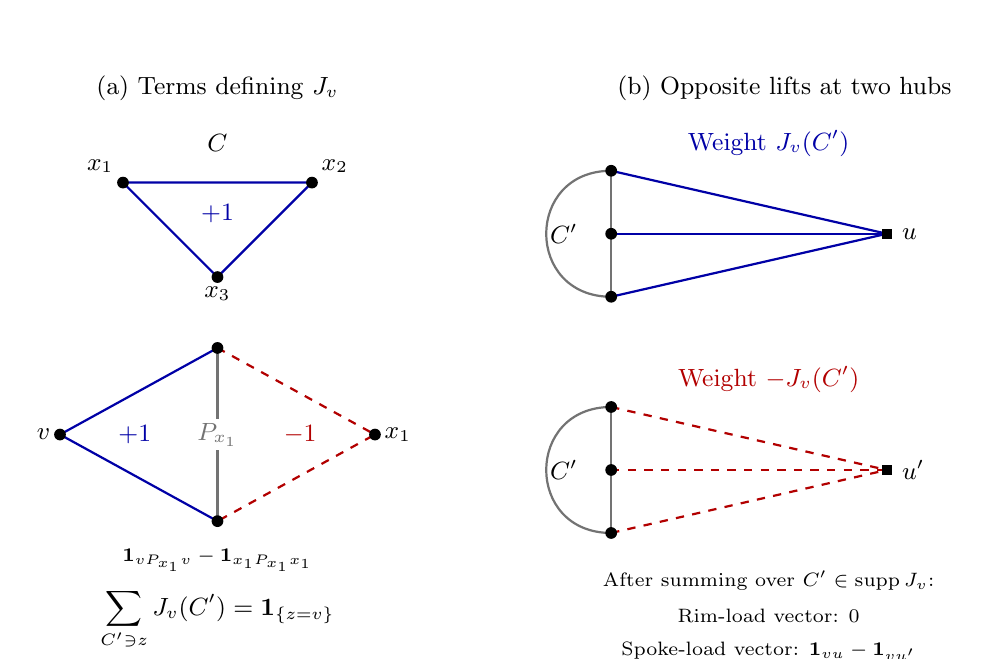
\begin{tikzpicture}[x=1cm,y=1cm,font=\small,
 dot/.style={circle,fill=black,inner sep=1.5pt},
 hub/.style={rectangle,fill=black,inner sep=1.8pt},
 positive/.style={blue!65!black,thick},
 negative/.style={red!70!black,thick,dashed},
 common/.style={black!55,thick},
 tag/.style={fill=white,inner sep=1.5pt}]
\node at (3,3.35) {(a) Terms defining $J_v$};
\node at (10.2,3.35) {(b) Opposite lifts at two hubs};

\coordinate (x1) at (1.8,2.15);
\coordinate (x2) at (4.2,2.15);
\coordinate (x3) at (3,.95);
\draw[positive] (x1)--(x2)--(x3)--cycle;
\foreach \q in {x1,x2,x3} {\node[dot] at (\q) {};}
\node[above left] at (x1) {$x_1$};
\node[above right] at (x2) {$x_2$};
\node[below] at (x3) {$x_3$};
\node at (3,2.65) {$C$};
\node[blue!65!black] at (3,1.75) {$+1$};

\coordinate (v) at (1,-1.05);
\coordinate (x) at (5,-1.05);
\coordinate (p) at (3,.05);
\coordinate (q) at (3,-2.15);
\draw[positive] (p)--(v)--(q);
\draw[negative] (p)--(x)--(q);
\draw[common] (p)--node[tag] {$P_{x_1}$} (q);
\foreach \z in {v,x,p,q} {\node[dot] at (\z) {};}
\node[left] at (v) {$v$};\node[right] at (x) {$x_1$};
\node[blue!65!black] at (1.95,-1.05) {$+1$};
\node[red!70!black] at (4.05,-1.05) {$-1$};
\node[font=\scriptsize] at (3,-2.65)
 {$\mathbf1_{vP_{x_1}v}-\mathbf1_{x_1P_{x_1}x_1}$};
\node at (3,-3.4)
 {$\displaystyle\sum_{C'\ni z}J_v(C')=\mathbf1_{\{z=v\}}$};

\foreach \shift/\hubname/\sign in {1.5/u/1,-1.5/{u'}/-1} {
\begin{scope}[shift={(0,\shift)}]
 \coordinate (a) at (8,.8);
 \coordinate (b) at (8,0);
 \coordinate (c) at (8,-.8);
 \coordinate (h) at (11.5,0);
 \draw[common] (a)--(b)--(c);
 \draw[common] (c) .. controls (6.9,-.8) and (6.9,.8) .. (a);
 \ifnum\sign=1
  \foreach \z in {a,b,c} {\draw[positive] (\z)--(h);}
  \node[blue!65!black] at (10,1.15) {Weight $J_v(C')$};
 \else
  \foreach \z in {a,b,c} {\draw[negative] (\z)--(h);}
  \node[red!70!black] at (10,1.15) {Weight $-J_v(C')$};
 \fi
 \foreach \z in {a,b,c} {\node[dot] at (\z) {};}
 \node[hub,label=right:$\hubname$] at (h) {};
 \node at (7.4,0) {$C'$};
\end{scope}
}
\node[font=\scriptsize] at (10,-2.9)
 {After summing over $C'\in\operatorname{supp}J_v$:};
\node[font=\scriptsize] at (10,-3.35) {Rim-load vector: $0$};
\node[font=\scriptsize] at (10,-3.8)
 {Spoke-load vector: $\mathbf1_{vu}-\mathbf1_{vu'}$};
\end{tikzpicture}
\caption{Constructing $J_v$ and lifting it with opposite signs to two hubs,
illustrated with $r=3$. Panel (a) shows the base cycle and one of the
three cycle differences, before multiplication by $1/r$.}
\label{fig:ordinary:spoke-load-transfer}
\end{figure}


For a wheel $W=W(C_W,h)$ with $h\in\{u,u'\}$,

\begin{equation}
 |T_{v,u,u'}(W)|\le C_5
 \left(\mathbf1_{\{v\in V(C_W)\}}n^{1-r}+n^{-r}\right).
 \label{eq:family:OF.A26}
\end{equation}

If $v\in V(C_W)$, the wheel fixes $r-1$ of the $r^2$ vertices in
$V(C)\cup\bigcup_{x\in V(C)}V(P_x)$, leaving $O_r(n^{r^2-r+1})$
configurations. If $v\notin V(C_W)$, it fixes $r$ of these vertices,
leaving $O_r(n^{r^2-r})$ configurations.
Each configuration contributes a coefficient of bounded absolute value.
Division by $|\mathcal T(v,u,u')|\ge\gamma n^{r^2}$ proves
\eqref{eq:family:OF.A26}. For $h\notin\{u,u'\}$ the coefficient is zero.

\paragraph{Correcting edge loads on $H$.}

After the correction on $E(Q)$, put $z_H(vu):=1-\mathcal L_H(\omega_0+\Psi_R)(vu)$.

The initial error bound and \eqref{eq:family:OF.A21} give $\|z_H\|_\infty\le C_6\eta$. By exact $Q$-edge loads and the assumed balance,

\begin{equation}
 \sum_{u\in N_H(v)}z_H(vu)
 =d_H(v)-\frac12d_Q(v)=0.
 \label{eq:family:OF.A27}
\end{equation}

Write $s_v:=d_H(v)$. By hypothesis, $s_v\ge\gamma n$. Define

\begin{equation*}
\Psi_H:=\sum_{v\in V}\frac1{s_v}
 \sum_{\substack{u,u'\in N_H(v)\\u\ne u'}}
 z_H(vu)T_{v,u,u'}.
\end{equation*}

At $vh\in E(H)$, \eqref{eq:family:OF.A25} and \eqref{eq:family:OF.A27} give

\begin{equation*}
\mathcal L_H\Psi_H(vh)
 =\frac{(s_v-1)z_H(vh)-\sum_{u\ne h}z_H(vu)}{s_v}
 =z_H(vh).
\end{equation*}

Every $Q$-edge load of $\Psi_H$ is zero.

Fix $W=W(C_W,h)$. For each $v$, at most $2s_v$ ordered pairs
$(u,u')$ with $h\in\{u,u'\}$ contribute to $\Psi_H(W)$.
Using $\|z_H\|_\infty\le C_6\eta$ and \eqref{eq:family:OF.A26}, we obtain
\begin{equation*}
 |\Psi_H(W)|\le 2C_5C_6\eta
 \sum_{v\in V}\left(\mathbf1_{\{v\in V(C_W)\}}n^{1-r}+n^{-r}\right).
\end{equation*}
Since $|V(C_W)|=r$, this gives

\begin{equation}
 |\Psi_H(W)|\le C_7\eta n^{1-r}.
 \label{eq:family:OF.A30}
\end{equation}

Set $\omega:=\omega_0+\Psi_R+\Psi_H$. Its rim and spoke loads
are exactly one. The constants $C_3,C_7$ in
\eqref{eq:family:OF.A20} and \eqref{eq:family:OF.A30} depend only
on $r,\vartheta,\alpha,\gamma,B_{\omega}$ and $k$.
We choose $\eta_0$ so that
$(C_3+C_7)\eta_0\le 1/(2B_{\omega})$. The two coefficient bounds follow
by adding the correction to the initial weights.
\end{proof}

\subsection{Potential wheel loads and configuration counts}
Let\phantomsection\label{gls:potential-ordinary-wheel-loads-and-configuration-counts} $r,k$ be integers with $r\ge3$ and $k\ge r+2$, and let
$\vartheta,\alpha>0$. Let $V,U$ be disjoint finite sets with $n:=|V|>0$, let $P,\mathcal F$
be graphs on $V$, and let $Q\subseteq P-E(\mathcal F)$ and
$H\subseteq V\times U$. Let $\mathcal W_P$ be the ordinary $r$-wheels
in $(P,V\times U)$ whose rim vertex sets are independent in
$\mathcal F$, and let $w_0:\mathcal W_P\to\mathbb R_{\ge0}$.
The graphs $P,\mathcal F$, the sets $V,U$, the family $\mathcal W_P$
and the function $w_0$ remain fixed when $Q,H$ change.
The following sums omit their indicated root edges,
which need not belong to $Q\cup H$. For $e\in E(P-E(\mathcal F))\cup(V\times U)$, let
\begin{equation}\label{eq:loads:ordinary-potential-seed}
    \widehat L_e(Q,H;w_0):=\sum_{\substack{W\in\mathcal W_P\\e\in E(W)}} w_0(W)\ind_{\{E(W)\setminus\{e\}\subseteq E(Q)\cup E(H)\}}.
\end{equation}
When $w_0$ is fixed, we write $\widehat L_e(Q,H):=\widehat L_e(Q,H;w_0)$.
For\phantomsection\label{gls:rim-load-correction-configurations:parent} $e=xy\in E(P-E(\mathcal F))$, let $\mathcal S_P(e)$ consist
of the sets $S\in\binom Vk$ such that
\begin{align*}
    \{x,y\}\subseteq S,\qquad E(\mathcal F[S])=\varnothing,\qquad \delta(P[S])\ge(\vartheta+\alpha/4)k.
\end{align*}
We\phantomsection\label{gls:potential-ordinary-wheel-loads-and-configuration-counts:rim-count} define
\begin{equation}\label{eq:loads:ordinary-potential-isolators}
    \widehat I_e(Q,H):=n^{-(k-1)}\sum_{u\in U}\sum_{S\in\mathcal S_P(e)} \ind_{\{E(P[S])\setminus\{e\}\subseteq E(Q)\}} \prod_{z\in S}\ind_{\{zu\in E(H)\}}.
\end{equation}
Let\phantomsection\label{gls:spoke-load-transfer-configurations:parent}\label{gls:potential-ordinary-wheel-loads-and-configuration-counts:transfer-count} $\mathcal T_P(v;u,u')$ be the family obtained from the definition of
$\mathcal T(v,u,u')$ by taking $Q=P-E(\mathcal F)$ and $H=V\times U$.
Each configuration includes its two root spokes $vu,vu'$. Let
\begin{equation}\label{eq:loads:ordinary-potential-transfers}
    \widehat T_{v,u,u'}(Q,H):=n^{-r^2} \sum_{C\in\mathcal T_P(v;u,u')} \ind_{\{C-\{vu,vu'\}\subseteq(Q,H)\}} \quad(v\in V,\ u\ne u'\in U).
\end{equation}
If $e\in E(Q)\cup E(H)$, then $\widehat L_e(Q,H)$ is the sum
of $w_0(W)$ over the wheels $W\subseteq(Q,H)$ containing $e$.
If $e\in E(Q)$, then $\widehat I_e(Q,H)$ is $n^{1-k}$ times the
number of pairs $(u,S)$ with $u\in U$, $S\in\mathcal S_P(e)$,
$P[S]\subseteq Q$ and $S\subseteq N_H(u)$.
If $vu,vu'\in E(H)$, then
$\widehat T_{v,u,u'}(Q,H)=n^{-r^2}|\mathcal T(v,u,u')|$.
In \eqref{eq:loads:ordinary-potential-isolators}, membership of the root
edge $e$ in $Q$ is not required, but every spoke $zu$ with $z\in S$
must belong to $H$.
\begin{lemma}
\label{lem:completion:ordinary-wheel-changes}
Let $r\ge3$ and $k\ge r+2$ be integers, and let $B_{\omega}>0$. There is
$C_{\rm stab}=C_{\rm stab}(r,k,B_{\omega})$ such that the following holds.
Let $\vartheta,\alpha>0$, let $P,\mathcal F$ be graphs on $V$,
let $U$ be disjoint from $V$, and
suppose $n=|V|>0$ and $|U|\le2n$.
Let $w_0:\mathcal W_P\to[0,B_{\omega}n^{1-r}]$.
Let $\mathcal Q=(Q,H)$ and $\widetilde{\mathcal Q}=(\widetilde Q,\widetilde H)$
be extended subgraphs of $(P-E(\mathcal F),V\times U)$.
If $t\ge0$ and $\Delta_*(\mathcal Q\triangle\widetilde{\mathcal Q})\le t$, then
\begin{align*}
    |\widehat L_e(\widetilde Q,\widetilde H;w_0)-\widehat L_e(Q,H;w_0)| &\le C_{\rm stab}t/n &&\bigl(e\in E(P-E(\mathcal F))\cup(V\times U)\bigr),\\
    |\widehat I_e(\widetilde Q,\widetilde H)-\widehat I_e(Q,H)| &\le C_{\rm stab}t/n &&\bigl(e\in E(P-E(\mathcal F))\bigr),\\
    |\widehat T_{v,u,u'}(\widetilde Q,\widetilde H)-\widehat T_{v,u,u'}(Q,H)| &\le C_{\rm stab}t/n &&\bigl(v\in V,\ u\ne u'\in U\bigr).
\end{align*}
\end{lemma}
\begin{proof}
We apply Lemma~\ref{lem:pr:weighted-count-change} with $a=n$ and
the following parameters. The normalizing powers of $n$ are
included in the coefficients.
\begin{equation*}
\begin{array}{c|c|c|c|c}
 \text{function}&f&q&J&B_Z\\\hline
 \widehat L_e&r-1&2r-1&2r!&B_{\omega}\\
 \widehat I_e&k-1&\binom{k}{2}-1+k&1&1\\
 \widehat T_{v,u,u'}&r^2&3r^2+3r&1&1
\end{array}
\end{equation*}
For a rim edge $e$, the sum defining $\widehat L_e$ has $r-2$
free rim vertices and one free hub; for a spoke $e$, it has
$r-1$ free rim vertices. In $\widehat I_{xy}$, the free labels
are the $k-2$ vertices of $S\setminus\{x,y\}$ and the hub.
Its required edges are
$(E(P[S])\setminus\{xy\})\cup\{zu:z\in S\}$: both $xu$ and $yu$
are required, but $xy$ is not. In $\widehat T_{v,u,u'}$, the
base cycle and replacement paths have $r^2$ free rim vertices.
Membership of $vu,vu'$ in $H$ is not required. For fixed free labels, the wheel
sum has at most $2r!$ cycle indices. In the other two sums, order
the set $S\setminus\{x,y\}$ using a fixed ordering of $V$, and
use the specified orderings of the base cycle and paths, respectively.
Each resulting tuple has at most one index, which gives $J=1$.
Thus every required edge has a free endpoint. Each free label
lies in $V$ or $U$, whose union has size at most $3n$.
The families determined by $P,\mathcal F$ and the coefficients $w_0$
are fixed in the two evaluations. One may therefore take $C_{\rm stab}:=K_{\rm prod} (\max\{r^2,k-1\}, \max\{3r^2+3r,\tbinom{k}{2}-1+k\},2r!,\max\{1,B_{\omega}\})$.
\end{proof}

\paragraph{Counts and loads after edge deletion.}
In the setting of Lemma~\ref{lem:completion:ordinary-wheel-changes},
let $F_Q\subseteq Q$, $F_H\subseteq H$ satisfy
$\Delta(F_Q\cup F_H)\le tn$, and let $Q^-:=Q-F_Q$, $H^-:=H-F_H$.
Let $w_0$ be a nonnegative weighting of the wheels in $\mathcal W_P$
contained in $(Q,H)$, with $w_0(W)\le B_{\omega}n^{1-r}$.
We extend $w_0$ by zero to $\mathcal W_P$ and keep this extension
fixed in both potential-load sums.
We write $\mathcal S_{(Q,H)}$ and $\mathcal T_{(Q,H)}$ for the
previously defined families evaluated in $(Q,H)$, keeping $P,\mathcal F$
fixed. With $C_S:=C_T:=C_L:=C_{\rm stab}(r,k,B_{\omega})$, the preceding lemma,
with $tn$ in place of its parameter $t$, and monotonicity give
\begin{equation}
\begin{aligned}
0\le{}&\sum_{u\in N_H(x)\cap N_H(y)}|\mathcal S_{(Q,H)}(xy,u)|
 -\sum_{u\in N_{H^-}(x)\cap N_{H^-}(y)}|\mathcal S_{(Q^-,H^-)}(xy,u)|
 \le C_Stn^{k-1} \quad(xy\in E(Q^-)),\\
0\le{}&|\mathcal T_{(Q,H)}(v,u,u')|-|\mathcal T_{(Q^-,H^-)}(v,u,u')|
 \le C_Ttn^{r^2}
 \quad(v\in V,\ u\ne u'\in N_{H^-}(v)),\\
0\le{}&\widehat L_e(Q,H;w_0)-\widehat L_e(Q^-,H^-;w_0)\le C_Lt
 \quad(e\in E(Q^-)\dot\cup E(H^-)).
\end{aligned}
\label{eq:packing:ordinary-deletion}
\end{equation}
The identities following \eqref{eq:loads:ordinary-potential-transfers}
identify these counts with their potential versions, since the specified
root edges survive in $(Q^-,H^-)$.

\section{Fractional marked \texorpdfstring{$c$}{c}-wheel decompositions with fixed types}

Under the hypotheses of Theorem~\ref{thm:weights:marked-numerical},
an initial weighting of the $(b,\pi)$-separated marked $c$-wheels
with loads close to one can be corrected to a fractional marked
$c$-wheel decomposition. The corrected weights remain between
positive constant multiples of $n^{1-c}$, where $n$ is the number
of rim vertices.

For a permutation $\pi$ of the rim vertex set, the physical images
of $(x\to y,0)$ and $(x\to y,K)$ are $\{x,y\}$ and
$\{x,\pi(y)\}$, respectively. A spoke $xu$ has physical image
$\{x,u\}$ in either type.

We first correct the rim loads by distributing signed cycle weights
over compatible hubs. We then correct the total spoke load at each
hub using cycles available at two hubs. Finally, common paths
realize alternating corrections on four spokes, analogous to the
four-edge corrections of
Montgomery~\cite[Lemma~4.3]{Montgomery2017Partite}.

\begin{definition}[Marked cycle and common-path families]\label{gls:compatible-hubs-and-common-marked-cycles}
\label{def:marked:common-paths}
Let $c\ge8$ and $b\ge0$ be integers. Let $V,W$ be disjoint finite sets,
$\pi$ a permutation of $V$, and $\mathcal Q=(R^0,R^K,H^0,H^K)$,
where $R^0,R^K$ are digraphs on $V$ and $H^0,H^K$ are edge-disjoint
bipartite graphs on $(V,W)$. Let $R:=R^0\dot\cup R^K$ and
$H:=H^0\dot\cup H^K$, with physical images as in
\eqref{eq:physical:image-map}. Let $\mathcal W(\mathcal Q):=\mathcal W_c^K(\mathcal Q;b,\pi)$.

\emph{Compatible hubs.} Let $\mathcal C_R$ consist of the directed $c$-cycles $C$ in $R$ with
one type-$K$ arc, a $(b,\pi)$-separated vertex set, $|\operatorname{phys}(E(C))|=c$
and $|\operatorname{phys}(e)|=2$ for every $e\in E(C)$.
The compatible hubs of $C\in\mathcal C_R$ form the set $W_C:=\{u\in W:W(C,u)\in\mathcal W(\mathcal Q)\}$. If
$W_C\ne\varnothing$, distributing a cycle weight equally over
the wheels $W(C,u)$ with $u\in W_C$ preserves its load on each rim edge.

\emph{Common cycles.}\phantomsection\label{gls:compatible-hubs-and-common-marked-cycles:common-cycles} For distinct $u,u'\in W$, their common marked cycles form the family
$\mathcal C(u,u'):=\{C\in\mathcal C_R:u,u'\in W_C\}$. For $C\in\mathcal C(u,u')$, the difference
$\mathbf1_{W(C,u)}-\mathbf1_{W(C,u')}$ has zero rim load.
At $u$ its total spoke load is $c-1$ in type $0$ and $1$ in type $K$, whereas
at $u'$ these two totals have the opposite signs.

\emph{Common paths.}\phantomsection\label{gls:common-path-families-for-marked-cycles-two-hubs} For any typed marked $c$-cycle $C$ on labels in $V$, let $t_C(v):=K$
at its marked head and $0$ elsewhere.

For $j\in\{0,K\}$, $v\in V$ and an ordered tuple
$\mathbf z=(z_1,\ldots,z_{c-1})$ of distinct labels in $V\setminus\{v\}$,
let $C_j(v,\mathbf z)$ be $vz_1\cdots z_{c-1}v$, with unique type-$K$
arc $z_{c-1}\to v$ when $j=K$, and $z_2\to z_3$ when $j=0$.
To realize an alternating correction on $vu,v'u,v'u',vu'$, we use
the cycles $C_j(v,\mathbf z)$ and $C_j(v',\mathbf z)$, which have
the common path $z_1\cdots z_{c-1}$.
For distinct $v,v'\in V$ and $u,u'\in W$, let
$\mathcal F_j(v,v';u,u')$ consist of the tuples $\mathbf z$ below.
For each tuple let $C_1:=C_j(v,\mathbf z)$ and $C_2:=C_j(v',\mathbf z)$.
The defining conditions are:
\begin{enumerate}[label=\textup{(\alph*)}]
\item the labels avoid $v,v'$, and both $C_j(v,\mathbf z)$ and
$C_j(v',\mathbf z)$ have their prescribed typed arcs in $R$;
\item $z_i u,z_i u'\in E(H^{t_{C_j(v,\mathbf z)}(z_i)})$ for every $i$;
\item $\operatorname{dist}_\pi(z_i,z_k)>b$ for $i\ne k$, and
$\operatorname{dist}_\pi(z_i,v),\operatorname{dist}_\pi(z_i,v')>b$ for every $i$;
\item $|\operatorname{phys}(E(C_\ell))|=c$ and $|\operatorname{phys}(e)|=2$ for
$\ell\in\{1,2\}$, $e\in E(C_\ell)$. Moreover,
\begin{equation*}
 \operatorname{phys}(e)=\operatorname{phys}(f)\ \Longrightarrow\
 (\operatorname{tail}(e),\operatorname{type}(e))
 =(\operatorname{tail}(f),\operatorname{type}(f))
 \quad(e\in E(C_1),\ f\in E(C_2)).
\end{equation*}
\end{enumerate}
The four root spokes $vu,vu',v'u,v'u'$ are not required to be present.
Moreover, no separation condition is imposed between $v$ and $v'$.
We call $\mathcal F_j(v,v';u,u')$ the common-path family for marked
cycles with roots $v,v';u,u'$ and root-spoke type $j\in\{0,K\}$.
\end{definition}
For comparisons of hosts, we write $W_C(\mathcal Q)$,
$\mathcal C(u,u';\mathcal Q)$ and $\mathcal F_j(v,v';u,u';\mathcal Q)$
for these same sets evaluated in $\mathcal Q$, keeping $c,b,\pi$ fixed.


If the four root spokes belong to $H^j$, every tuple in
$\mathcal F_j(v,v';u,u')$ gives four members of $\mathcal W(\mathcal Q)$,
by using either rooted cycle with either hub.
For a signed weighting $\psi:\mathcal W(\mathcal Q)\to\mathbb R$, we write
\begin{equation*}
L_\psi(e):=\sum_{\substack{W'\in\mathcal W(\mathcal Q)\\e\in E_{\rm phys}(W')}}
                  \psi(W')
 \quad\bigl(e\in E_{\rm phys}(\mathcal Q)\bigr).
\end{equation*}

\Needspace{8\baselineskip}
\begin{definition}[Marked host estimates]\label{gls:marked-host-estimates}
Let $V,W$ be disjoint nonempty sets, $|V|=n$, and let $\pi$ be a permutation of $V$.
Let $\mathcal Q=(R^0,R^K,H^0,H^K)$, where the rim graphs are digraphs
on $V$ and the spoke graphs are edge-disjoint bipartite graphs on $(V,W)$.
Let $R:=R^0\dot\cup R^K$ and $H:=H^0\dot\cup H^K$.
Let $c\ge8$, $b\ge1$ and $D_{\rm exc}\ge0$ be integers,
and let $D,p>0$ and $\varsigma_0,\varsigma_K\in(0,1]$.
Let $\mathcal C_R$, $W_C$, $\mathcal C(u,u')$ and
$\mathcal F_j(v,v';u,u')$ be the families of
Definition~\ref{def:marked:common-paths} for these $c,b,\pi,\mathcal Q$.
Let $\varepsilon,\delta\ge0$, $\beta,\tau,h>0$ and $0<\delta_{\rm cut}<1/4$.
We say that $(\mathcal Q,(\varsigma_j))$ has
\emph{$(b,\pi)$-separated marked host estimates} with target rim degrees
$pD$ and $pD/(c-1)$, errors $(\varepsilon,\delta)$, extension coefficient
$\beta$, rim bounds $(\tau,\delta_{\rm cut},h)$ and exception bound
$D_{\rm exc}$ if the following hold.
\begin{enumerate}[label=\textup{(MH\arabic*)}]
\item\label{item:mw:rim} \emph{Rim degrees and cuts.}
\begin{equation*}
\begin{gathered}
 d^\pm_{R^0}(v)=pD\pm \varepsilon n,\qquad
 d^\pm_{R^K}(v)=pD/(c-1)\pm \varepsilon n\quad(v\in V),\\
 |N^+_{R^0}(x)\cap N^-_{R^0}(y)|\ge\tau n\quad(x\ne y\in V).
\end{gathered}
\end{equation*}
Let $D_{R^0}$ be the bipartite representation of $R^0$, with tail
and head classes $V_{\rm out},V_{\rm in}$, both copies of $V$.
For all $X\subseteq V_{\rm out}$ and $Y\subseteq V_{\rm in}$ with
$|X|+|Y|>(1-2\delta_{\rm cut})n$, we have
\begin{equation*}
 e_{D_{R^0}}(X,Y)\ge h n\min\{|X|,|Y|\}.
\end{equation*}
\item\label{item:mw:extensions} \emph{Compatible hubs, common cycles and common paths.}
\begin{equation*}
 |W_C|\ge\beta n\quad(C\in\mathcal C_R),\qquad
 |\mathcal C(u,u')|\ge\beta n^c\quad(u\ne u'\in W).
\end{equation*}
For $j\in\{0,K\}$, distinct $v,v'\in V$ and distinct $u,u'\in W$,
\begin{equation*}
 vu,vu',v'u,v'u'\in E(H^j)
 \quad\Longrightarrow\quad
 |\mathcal F_j(v,v';u,u')|\ge\beta n^{c-1}.
\end{equation*}
\item\label{item:mw:spokes} \emph{Spoke intersections.}
For $j\in\{0,K\}$ and $S\subseteq W$ with $1\le|S|\le3$,
\begin{equation*}
 \left|\bigcap_{u\in S}N_{H^j}(u)\right|=\varsigma_j^{|S|}n\pm \delta n.
\end{equation*}
For every $j\in\{0,K\}$ and $x\in V$ there is
$E_x^j\subseteq V$, $|E_x^j|\le D_{\rm exc}$,
such that
\begin{equation*}
 |N_{H^j}(x)\cap N_{H^j}(y)|=\varsigma_j^2|W|\pm \delta\varsigma_j^2|W|\quad(y\in V\setminus E_x^j).
\end{equation*}
\end{enumerate}
\end{definition}

In the following proof, \ref{item:mw:rim} permits the signed rim
correction by Theorem~\ref{thm:capacity:marked-numerical}.
The bounds in \ref{item:mw:extensions} allow us to distribute the
weight of each cycle $C$ among the wheels $W(C,u)$ with $u\in W_C$,
transfer total spoke load between hubs using
$\mathcal C(u,u')$, and use $\mathcal F_j(v,v';u,u')$ to construct
signed wheel weightings with alternating loads on $vu,v'u,v'u',vu'$
and zero rim load whenever all four root spokes belong to $H^j$.
Condition \ref{item:mw:spokes} permits
Lemma~\ref{lem:four:sparse-alternating} to express each remaining
spoke error as a bounded sum of these alternating corrections.

\begin{theorem}[Fractional marked wheel decompositions]
\label{thm:weights:marked-numerical}
Let $\alpha,p_{\rm rim},p_*,\beta,\omega_W>0$ and $B_{\omega}>1$, with
$\alpha<1/4$ and $p_{\rm rim}<1/2$.
Let $c\ge\max\{8,c_0(\alpha,p_{\rm rim})\}$ be even, where $c_0$ is from
Theorem~\ref{thm:capacity:marked-numerical}. There are
$\varepsilon_*,\eta_*,\delta_*>0$ such that for every integer $b\ge2$
there is $n_0\in\mathbb N$ for which the following holds for every
integer $n\ge n_0$ and every $p\in[p_{\rm rim},1/2)$.

Let $\delta_c:=\min\{\alpha/16,p/128\}$ and $h_c:=\alpha p/16$.
Let $\mathcal Q=(R^0,R^K,H^0,H^K)$ be a typed extended graph on $(V,W,\pi)$,
where $\pi:V\to V$ is a permutation, $|V|=n$ and $\omega_Wn\le|W|\le n$, with disjoint spoke types
and injective rim physical map \eqref{eq:physical:image-map}.
Let $\varsigma_0,\varsigma_K\in[p_*,1]$, $\delta\ge0$, $D_{\rm exc}\in\mathbb Z_{\ge0}$,
and let $R:=R^0\dot\cup R^K$, $H:=H^0\dot\cup H^K$ and
$\mathcal W(\mathcal Q):=\mathcal W_c^K(\mathcal Q;b,\pi)$.
Assume that $(\mathcal Q,(\varsigma_j))$ has $(b,\pi)$-separated marked
host estimates with target rim degrees $pD$ and $pD/(c-1)$ for some
$D\in[n/2,2n]$, errors $(\varepsilon_*,\delta)$, extension coefficient
$\beta$, rim bounds $(\alpha p^2,\delta_c,h_c)$ and exception bound $D_{\rm exc}$.
Let $\omega_0:\mathcal W(\mathcal Q)\to\mathbb R_{\ge0}$ satisfy
\begin{equation}
\label{eq:marked:initial-weights}
 B_{\omega}^{-1}n^{1-c}\le\omega_0(W')\le B_{\omega}n^{1-c}
 \quad(W'\in\mathcal W(\mathcal Q)),\qquad
 L_{\omega_0}(e)=1\pm \eta_*\quad(e\in E_{\rm phys}(\mathcal Q)).
\end{equation}
Suppose also
\begin{equation}
 \delta+D_{\rm exc}/n+1/|W|\le\delta_*,
 \label{eq:marked:spoke-budget}
\end{equation}
and, for every $v\in V$ and $u\in W$,
\begin{equation}
 d_R^+(v)=d_R^-(v)=d_H(v),\quad d_{R^K}^-(v)=d_{H^K}(v),\quad
 d_{H^0}(u)=(c-1)d_{H^K}(u).
 \label{eq:marked:exact-degrees}
\end{equation}
Then there exists $\omega:\mathcal W(\mathcal Q)\to\mathbb R_{\ge0}$ such that
\begin{equation}
 L_\omega(e)=1\quad(e\in E_{\rm phys}(\mathcal Q)),\qquad
 \frac{n^{1-c}}{2B_{\omega}}\le\omega(W')\le2B_{\omega} n^{1-c}
                 \quad(W'\in\mathcal W(\mathcal Q)).
 \label{eq:marked:exact-weights}
\end{equation}
\end{theorem}
\begin{proof}
Let $\varepsilon_{\rm cap},\kappa_{\rm cap},B_{\rm cap}$ be
the corresponding constants supplied by Theorem~\ref{thm:capacity:marked-numerical}
for $\alpha,p_{\rm rim},c$, decreasing $\kappa_{\rm cap}$ below one if necessary.
Let $\delta_{\rm alt},C_{\rm alt}$ be supplied by
Lemma~\ref{lem:four:sparse-alternating} for $p_*$.
We choose auxiliary constants with
\begin{equation*}
0<\eta_*\ll\delta_*\ll\varepsilon_* \ll\varepsilon_{\rm cap},\delta_{\rm alt},\kappa_{\rm cap}, 1/B_{\rm cap},1/C_{\rm alt},\alpha,p_{\rm rim},p_*,\beta,1/B_{\omega},1/c.
\end{equation*}
We use the physical map $\operatorname{phys}$ from \eqref{eq:physical:image-map}.
All constants $C_i$ below depend only on
$\alpha,p_{\rm rim},p_*,\beta,c$, and not on $p,b,\delta,D_{\rm exc}$.

Put $\eta:=\max_{e\in E_{\rm phys}(\mathcal Q)}|L_{\omega_0}(e)-1|$.
By \eqref{eq:marked:initial-weights}, every physical edge has positive
$\omega_0$-load. Since $\operatorname{phys}$ is injective on $E(R)$, every arc of $R$
belongs to a wheel in $\mathcal W(\mathcal Q)$. Thus its physical
image is loopless and its auxiliary endpoints are $(b,\pi)$-separated.
This verifies the arc conditions of
Theorem~\ref{thm:capacity:marked-numerical}.
If $\eta=0$, take $\omega:=\omega_0$. Assume $\eta>0$.

\paragraph{Step 1: Correcting the rim loads.}
The hierarchy gives $\varepsilon_*\le\varepsilon_{\rm cap}$.
We take $n_0$ at least the order threshold in
Theorem~\ref{thm:capacity:marked-numerical} for $b$.
Define $z_R(e):=1-L_{\omega_0}(\operatorname{phys}(e))$ for $e\in E(R)$.
Equation~\eqref{eq:marked:exact-degrees} gives $d_R^+=d_R^-$ and
$|E(R^0)|=(c-1)|E(R^K)|$, the latter by summing the spoke identities.
Hence the all-ones vector $\mathbf1\in\mathbb R^{E(R)}$ satisfies
\eqref{eq:capacity:balance}.
Every wheel has one incoming and one outgoing rim arc at each of its
labels, and has $c-1$ unmarked arcs and one marked arc.
Its rim-load vector satisfies the same equations, so $z_R$ does too.
Also $\|z_R\|_\infty\le\eta$.
We apply Theorem~\ref{thm:capacity:marked-numerical} to the same $R^0,R^K$
and to capacities $\mathbf1$ and
$\mathbf1+\kappa_{\rm cap}z_R/\eta$, using
\ref{item:mw:rim}. Both capacity vectors are nonnegative,
satisfy \eqref{eq:capacity:balance}, and lie within $\kappa_{\rm cap}$
of $\mathbf1$. Let $\lambda_0$ and $\lambda_1$ be the cycle
weightings for these two capacities, respectively. Then
$\psi:=(\eta/\kappa_{\rm cap})(\lambda_1-\lambda_0)$ is a signed
weighting on $\mathcal C_R$ with rim loads $z_R$ and
$|\psi(C)|\le C_1\eta n^{2-c}$, where
$C_1:=2B_{\rm cap}/\kappa_{\rm cap}$.

\paragraph{Step 2: Lifting the cycle weights to marked wheels.}
Set $\Psi_R(W(C,u)):=\psi(C)/|W_C|$ for $u\in W_C$.
The bound $|W_C|\ge\beta n$ in \ref{item:mw:extensions} gives
$|\Psi_R(W')|\le C_2\eta n^{1-c}$ with $C_2:=C_1/\beta$.
Its rim loads equal $z_R$.
A fixed spoke $vu$ belongs to at most $c n^{c-1}$ marked wheels:
fix the position of $v$ relative to the unique marked arc, then choose
the other $c-1$ labels. Thus
$|L_{\Psi_R}(vu)|\le C_3\eta$, where $C_3:=cC_2$.

\paragraph{Step 3: Correcting the total spoke load at each hub.}
For $vu\in E(H^j)$ put $z_j(vu):=1-L_{\omega_0+\Psi_R}(vu)$,
and extend $z_j$ by zero to missing pairs.
Then $\|z_j\|_\infty\le C_4\eta$, where $C_4:=1+C_3$.
At $v\in V$, a wheel has one marked spoke exactly when its rim has a
marked arc entering $v$, and one spoke of either type exactly when
its rim has an arc leaving $v$.
Since $\omega_0+\Psi_R$ has unit rim loads,
\begin{equation*}
 \sum_{u\in W}z_K(vu)=d_{H^K}(v)-d_{R^K}^-(v)=0,\qquad
 \sum_{u\in W}(z_0(vu)+z_K(vu))=d_H(v)-d_R^+(v)=0,
\end{equation*}
where the equalities use \eqref{eq:marked:exact-degrees}.
Consequently $\sum_{u\in W}z_j(vu)=0$ for every $v\in V$ and $j\in\{0,K\}$. At $u\in W$, the last
identity in \eqref{eq:marked:exact-degrees}, and the $c-1$ to one
spoke ratio in each wheel, give
\begin{equation}
 \sum_vz_0(vu)=(c-1)\sum_vz_K(vu).
 \tag{W2}\label{eq:marked:column-ratio}
\end{equation}
For distinct $u,u'\in W$ define
\begin{equation*}
 \Gamma_{u,u'}:=
 \frac1{|\mathcal C(u,u')|}\sum_{C\in\mathcal C(u,u')}
       \bigl(\ind_{W(C,u)}-\ind_{W(C,u')}\bigr).
\end{equation*}
For every $e\in\operatorname{phys}(E(R))$ and every $v\in V$, $j\in\{0,K\}$,
$L_{\Gamma_{u,u'}}(e)=0$ and $\sum_{w\in N_{H^j}(v)}L_{\Gamma_{u,u'}}(vw)=0$. For every $w\in W$, its total
spoke loads are
\begin{equation*}
 \sum_{v\in N_{H^K}(w)}L_{\Gamma_{u,u'}}(vw)
 =\mathbf1_{\{w=u\}}-\mathbf1_{\{w=u'\}},\qquad
 \sum_{v\in N_{H^0}(w)}L_{\Gamma_{u,u'}}(vw)
 =(c-1)(\mathbf1_{\{w=u\}}-\mathbf1_{\{w=u'\}}).
\end{equation*}
The bound $|\mathcal C(u,u')|\ge\beta n^c$ in
\ref{item:mw:extensions} bounds every coefficient of $\Gamma_{u,u'}$
in absolute value by $\beta^{-1}n^{-c}$. Since at most $c n^{c-1}$ cycles
contain a fixed rim vertex, every spoke load of $\Gamma_{u,u'}$ has
absolute value at most $c/(\beta n)$.

Put $B(u):=\sum_vz_K(vu)$ and $s:=|W|$. Then $\sum_uB(u)=0$ and
$|B(u)|\le C_4\eta n$. Define $\Psi_{\rm col}:=\frac1s\sum_{u\ne u'}B(u)\Gamma_{u,u'}$. For every $u\in W$,
\begin{equation*}
\begin{aligned}
 \sum_{v\in N_{H^K}(u)}L_{\Psi_{\rm col}}(vu)
 &=\frac{(s-1)B(u)-\sum_{u'\ne u}B(u')}{s}=B(u),\\
 \sum_{v\in N_{H^0}(u)}L_{\Psi_{\rm col}}(vu)
 &=(c-1)B(u)=\sum_{v\in V}z_0(vu).
\end{aligned}
\end{equation*}
The last equality uses \eqref{eq:marked:column-ratio}.
Also $L_{\Psi_{\rm col}}(e)=0$ for every rim edge $e$, and
$\sum_{u\in N_{H^j}(v)}L_{\Psi_{\rm col}}(vu)=0$ for $v\in V$, $j\in\{0,K\}$.
At a fixed wheel or spoke, only ordered pairs containing its hub
contribute. There are at most $2(s-1)$ such pairs. The preceding
bounds therefore give
$|\Psi_{\rm col}(W')|\le C_6\eta n^{1-c}$ and
$|L_{\Psi_{\rm col}}(vu)|\le C_6\eta$, with $C_6:=2cC_4/\beta$.

\paragraph{Step 4: Correcting the remaining spoke errors.}
The hierarchy gives $\delta_*\le\delta_{\rm alt}/2$, and we increase $n_0$
so that $1/n\le\delta_{\rm alt}/2$ for $n\ge n_0$.
We extend $r_j:=z_j-L_{\Psi_{\rm col}}|_{E(H^j)}$ by zero outside $E(H^j)$.
For $j\in\{0,K\}$, these functions satisfy
\begin{equation*}
 \sum_{u\in W}r_j(vu)=0\ (v\in V),\qquad
 \sum_{v\in V}r_j(vu)=0\ (u\in W),\qquad
 \|r_j\|_\infty\le C_7\eta,\quad C_7:=C_4+C_6.
\end{equation*}
We apply Lemma~\ref{lem:four:sparse-alternating} to $H^j$ with
$A=V$, $B=W$, $p=\varsigma_j$, exception-bound parameter
$D=\max\{1,D_{\rm exc}\}$ and signed function $z=r_j$. The intersection bounds in
\ref{item:mw:spokes} are its hypotheses \textup{(i)}--\textup{(iii)}
with the same $\delta$. By \eqref{eq:marked:spoke-budget},
$\delta+\max\{1,D_{\rm exc}\}/n+1/|W|\le\delta_*+1/n\le\delta_{\rm alt}$. It gives coefficients $a_j(Q)$ on ordered four-cycles of
$H^j$ such that
\begin{equation}
 r_j=\sum_Q a_j(Q)\delta_Q,\qquad
 \sum_{Q\ni e}|a_j(Q)|\le C_8\eta\quad(e\in E(H^j)),
 \qquad C_8:=C_{\rm alt}C_7.
 \label{eq:marked:alternating-load}
\end{equation}
For an ordered four-cycle $Q=(v,u,v',u')$ of $H^j$, all four
spokes $vu,v'u,v'u',vu'$ belong to $H^j$. Hence
\ref{item:mw:extensions} gives
$|\mathcal F_j(v,v';u,u')|\ge\beta n^{c-1}$.
Each tuple in this family gives four wheels in $\mathcal W(\mathcal Q)$.
Let $\Theta_{j,Q}$ be the average, over these tuples, of
\begin{equation*}
 \ind_{W(C_j(v,\mathbf z),u)}-
 \ind_{W(C_j(v',\mathbf z),u)}+
 \ind_{W(C_j(v',\mathbf z),u')}-
 \ind_{W(C_j(v,\mathbf z),u')}.
\end{equation*}
Its rim loads cancel, and its spoke-load vector is
$\delta_Q=\ind_{vu}-\ind_{v'u}+\ind_{v'u'}-\ind_{vu'}$ in type $j$,
with zero load on every spoke at a free label.

Figure~\ref{fig:marked:four-wheel-correction} shows these cancellations.
\begin{figure}[htbp]
\centering
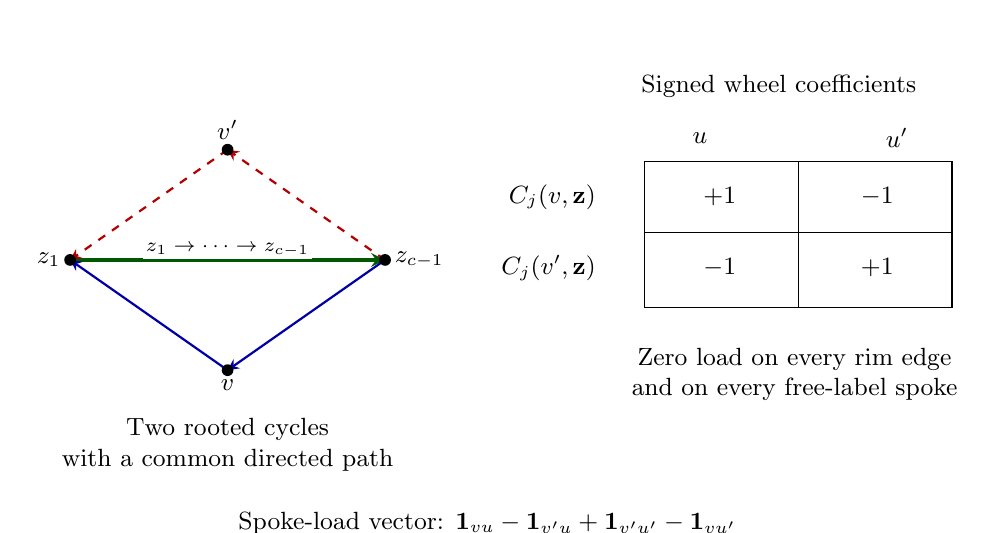
\begin{tikzpicture}[x=1cm,y=1cm,font=\small,>=stealth,
 dot/.style={circle,fill=black,inner sep=1.5pt},
 first/.style={blue!65!black,thick},
 second/.style={red!70!black,thick,dashed},
 shared/.style={green!35!black,very thick},
 spoke/.style={black!45,thin},
 tag/.style={fill=white,inner sep=1pt,font=\scriptsize}]

\coordinate (a) at (-2,0); \coordinate (b) at (2,0);
\coordinate (v) at (0,-1.4); \coordinate (vp) at (0,1.4);
\draw[shared,->] (a)--(b);
\draw[first,->] (v)--(a); \draw[first,->] (b)--(v);
\draw[second,->] (vp)--(a); \draw[second,->] (b)--(vp);
\foreach \n in {a,b,v,vp} {\node[dot] at (\n) {};}
\node[left] at (a) {$z_1$}; \node[right] at (b) {$z_{c-1}$};
\node[below] at (v) {$v$}; \node[above] at (vp) {$v'$};
\node[tag,above] at (0,0) {$z_1\to\cdots\to z_{c-1}$};
\node[align=center] at (0,-2.35) {Two rooted cycles\\with a common directed path};
\node at (7,2.2) {Signed wheel coefficients};
\node at (6,1.55) {$u$}; \node at (8.5,1.55) {$u'$};
\node[anchor=east] at (4.8,.8) {$C_j(v,\mathbf z)$};
\node[anchor=east] at (4.8,-.1) {$C_j(v',\mathbf z)$};
\draw (5.3,-.6) rectangle (9.2,1.25);
\draw (7.25,-.6)--(7.25,1.25); \draw (5.3,.35)--(9.2,.35);
\node at (6.25,.8) {$+1$}; \node at (8.25,.8) {$-1$};
\node at (6.25,-.1) {$-1$}; \node at (8.25,-.1) {$+1$};
\node[align=center] at (7.2,-1.45) {Zero load on every rim edge\\and on every free-label spoke};
\node at (3.3,-3.35)
 {Spoke-load vector: $\mathbf1_{vu}-\mathbf1_{v'u}+\mathbf1_{v'u'}-\mathbf1_{vu'}$};

\end{tikzpicture}
\caption{The four-wheel correction associated with
$\mathbf z\in\mathcal F_j(v,v';u,u')$, when all four root spokes lie in $H^j$.
Opposite signs cancel the loads on rim edges and spokes at free labels,
leaving only the displayed root-spoke loads.
Type labels are omitted from the left panel.}
\label{fig:marked:four-wheel-correction}
\end{figure}
 The lower bound
on $|\mathcal F_j(v,v';u,u')|$ and the at most $4c$
representations of a fixed wheel for a fixed $Q$ give
$|\Theta_{j,Q}(W')|\le C_9n^{1-c}$, with $C_9:=4c/\beta$.
Whenever this coefficient is nonzero, $Q$ contains a spoke of $W'$.
Equation~\eqref{eq:marked:alternating-load} therefore gives
\begin{equation*}
 \left|\sum_{j,Q}a_j(Q)\Theta_{j,Q}(W')\right|
 \le C_9n^{1-c}\sum_{e\in E(H)\cap E_{\rm phys}(W')}
                          \sum_{Q\ni e}|a_{\operatorname{type}(e)}(Q)|
 \le cC_8C_9\eta n^{1-c}.
\end{equation*}
Write $\Psi_{\rm alt}:=\sum_{j,Q}a_j(Q)\Theta_{j,Q}$.
It has zero rim loads and spoke loads $r_j$ on $H^j$.

\paragraph{Step 5: Positivity of the coefficients.}
Set $\omega:=\omega_0+\Psi_R+\Psi_{\rm col}+\Psi_{\rm alt}$.
The load equalities in Steps 2--4 give $L_\omega(e)=1$ for all
$e\in E_{\rm phys}(\mathcal Q)$. Their coefficient bounds give
\begin{equation*}
 |\omega(W')-\omega_0(W')|\le K_{\rm err}\eta n^{1-c},\qquad
 K_{\rm err}:=C_2+C_6+cC_8C_9.
\end{equation*}
The hierarchy gives $K_{\rm err}\eta_*\le 1/(2B_{\omega})$.
Since $B_{\omega}+1/(2B_{\omega})\le2B_{\omega}$, these bounds and
\eqref{eq:marked:initial-weights} prove \eqref{eq:marked:exact-weights}.
\end{proof}

\begin{definition}[Potential marked wheel loads]\label{gls:potential-marked-wheel-loads}
\label{def:marked:potential-loads}
Let $c\ge8$ and $b\ge0$ be integers, let $V,W$ be disjoint finite sets,
let $P$ be a simple graph on $V$, and let $\pi$ be a permutation of $V$. In the following
formulas typed arcs and spokes are
occurrences, not their unordered physical images. The map
\eqref{eq:physical:image-map} is defined on all triples $(x,y,j)$ with
$x,y\in V$ and $j\in\{0,K\}$.
The potential occurrences are
\begin{equation*}
 \mathfrak E_P:=
 \{(x,y,j):x,y\in V,\ j\in\{0,K\},\ \operatorname{phys}(x,y,j)\in E(P)\}
 \dot\cup (V\times W\times\{0,K\}).
\end{equation*}
Let $E(\mathcal Q)\subseteq\mathfrak E_P$.
Let $\mathcal W_P$ be a family of typed marked $c$-wheels in $\mathfrak E_P$,
each with distinct loopless physical edges and satisfying any specified
separation restriction, and let $w_0:\mathcal W_P\to\mathbb R_{\ge0}$.

For $e\in\mathfrak E_P$, we define
\begin{equation}
 \widehat L_e(\mathcal Q;w_0):=
 \sum_{\substack{W'\in\mathcal W_P\\e\in E(W')}}w_0(W')
       \prod_{f\in E(W')\setminus\{e\}}\ind_{\{f\in E(\mathcal Q)\}}.
 \label{eq:loads:marked-potential-seed}
\end{equation}
When $w_0$ is fixed, we write $\widehat L_e(\mathcal Q):=\widehat L_e(\mathcal Q;w_0)$.
The product omits precisely the indicator $\ind_{\{e\in E(\mathcal Q)\}}$
of the root occurrence.
The formula is defined even when $e\notin E(\mathcal Q)$, and does
not require the physical image map to be injective on all of $E(\mathcal Q)$.
For\phantomsection\label{gls:potential-compatible-hub-count} a $(b,\pi)$-separated typed marked cycle $C$ whose physical
rim edges are distinct, loopless and contained in $P$, let
\begin{equation*}
\widehat H_C(\mathcal Q):=\sum_{u\in W}\prod_{v\in V(C)}
            \ind_{\{(v,u,t_C(v))\in E(\mathcal Q)\}}.
\end{equation*}
No rim indicator occurs in this product. Membership in
$\mathcal F_j(v,v';u,u')$ does not require the four root spokes to be
present, whereas a cycle in $\mathcal C(u,u')$ requires all its rim arcs
and spokes at both hubs.
The potential occurrences $\mathfrak E_P$, wheel family $\mathcal W_P$
and function $w_0$ remain fixed as $\mathcal Q$ varies. 
\end{definition}
\Needspace{14\baselineskip}
\begin{lemma}
\label{lem:completion:marked-wheel-changes}
Let $c\ge8$ be an even integer and let $B_{\omega}>0$. There is
$C_{\rm stab}=C_{\rm stab}(c,B_{\omega})$ such that the following holds for every integer $b\ge0$.
Let $P$ be a graph on $V$, let $\pi$ be a permutation of $V$,
and let $W$ be disjoint from $V$, with $n=|V|>0$ and $|W|\le2n$.
Let $\mathcal Q=(R^0,R^K,H^0,H^K)$ and
$\widetilde{\mathcal Q}=(\widetilde R^0,\widetilde R^K,
\widetilde H^0,\widetilde H^K)$ have edge sets in $\mathfrak E_P$, with
$E(H^0)\cap E(H^K)=E(\widetilde H^0)\cap E(\widetilde H^K)=\varnothing$.
Let $w_0:\mathcal W_P\to[0,B_{\omega}n^{1-c}]$, where $\mathfrak E_P$
and $\mathcal W_P$ are defined in Definition~\ref{def:marked:potential-loads}.
The families $\mathcal C(u,u')$ and $\mathcal F_j(v,v';u,u')$ in
$\mathcal Q$ and $\widetilde{\mathcal Q}$ are defined with the same $c,b,\pi$.
Suppose $t\ge0$ and
$\Delta_*(\mathcal Q\triangle\widetilde{\mathcal Q})\le t$.
Then
\begin{equation*}
\begin{aligned}
 |\widehat L_e(\widetilde{\mathcal Q};w_0)-\widehat L_e(\mathcal Q;w_0)|
 &\le C_{\rm stab}t/n &&(e\in\mathfrak E_P),\\
 \bigl||\mathcal C(u,u';\widetilde{\mathcal Q})|
             -|\mathcal C(u,u';\mathcal Q)|\bigr|
 &\le C_{\rm stab}t n^{c-1} &&(u\ne u'\in W),\\
 \bigl||\mathcal F_j(v,v';u,u';\widetilde{\mathcal Q})|
             -|\mathcal F_j(v,v';u,u';\mathcal Q)|\bigr|
 &\le C_{\rm stab}t n^{c-2}
 &&\substack{v\ne v'\in V,\ u\ne u'\in W,\\j\in\{0,K\}}.
\end{aligned}
\end{equation*}
\end{lemma}
\begin{proof}
We apply Lemma~\ref{lem:pr:weighted-count-change} with $a=n$:
\begin{equation*}
\begin{array}{c|c|c|c|c}
 \text{function}&f&q&J&B_Z\\\hline
 \widehat L_e&c-1&2c-1&2c!&B_{\omega}\\
 n^{-c}|\mathcal C(u,u';\mathcal Q)|&c&3c&2c!&1\\
 n^{1-c}|\mathcal F_j(v,v';u,u';\mathcal Q)|&c-1&4c&1&1
\end{array}
\end{equation*}
For $\widehat L_e$, the free labels are $c-2$ rim vertices and
one hub when $e$ is a rim arc, and $c-1$ rim vertices when $e$
is a spoke. The count $|\mathcal C(u,u';\mathcal Q)|$ requires all
rim arcs and spokes of each cycle at both hubs. The count
$|\mathcal F_j(v,v';u,u';\mathcal Q)|$ does not require the root spokes
$vu,v'u,vu',v'u'$ to be present.
In each sum every required occurrence has a free endpoint.
For the common-cycle and common-path counts, the index sets consist
of all cycles or tuples satisfying the prescribed type, separation
and physical-image conditions. These index sets are fixed for
$\mathcal Q$ and $\widetilde{\mathcal Q}$, while the respective
indicator products impose the presence of the required arcs and
spokes in each graph. The potential wheel family $\mathcal W_P$
and its coefficients $w_0$ are also fixed.
Since $|W|\le2n$, one may take
$C_{\rm stab}:=K_{\rm prod}(c,4c,2c!,\max\{1,B_{\omega}\})$.
The symmetric difference consists of typed occurrences: a type
change contributes both the removed and the inserted occurrence.
No injectivity of the physical image map on
$E(\mathcal Q)\cup E(\widetilde{\mathcal Q})$ is used.
\end{proof}

\section{Divisibility correction without changing types}
We delete a subgraph of small maximum auxiliary and physical incidence
degree to make the four marked wheel degree identities exact. The deletion preserves the direction and type of every
remaining edge. The permutation $\pi$ may act on a larger ambient set
$V^*\supseteq V$, and we do not assume $\pi(V)=V$.

\paragraph{The four degree differences.}
Let\phantomsection\label{gls:restricted-balance-differences:unrestricted} $c\ge4$ be an integer and let $V,W$ be disjoint finite sets.
For digraphs $R^0,R^K$ on $V$ and
bipartite graphs $H^0,H^K$ on $(V,W)$, we write
$\mathcal Q:=(R^0,R^K,H^0,H^K)$. Unions of different types below are
disjoint unions of edge occurrences. Let
\begin{equation}
\begin{split}
 a^+(v)&:=d^+_{R^0}(v)+d^+_{R^K}(v)-d_{H^0}(v)-d_{H^K}(v),\\
 a^-(v)&:=d^-_{R^0}(v)+d^-_{R^K}(v)-d_{H^0}(v)-d_{H^K}(v),\\
 a^K(v)&:=d^-_{R^K}(v)-d_{H^K}(v)\qquad(v\in V),\\
 a^W(w)&:=d_{H^0}(w)-(c-1)d_{H^K}(w)\qquad(w\in W).
\end{split}
\tag{T2}\label{eq:typed:imbalance}
\end{equation}
Thus marked $c$-wheel divisibility is the vanishing of these four
functions. Recall from \eqref{eq:digraph:bipartite-representation}
that, for a directed multigraph $R$, the bipartite graph $D_R$ has
a tail copy and a head copy of $V(R)$. The bijection $\beta_R$
maps each arc occurrence $x\to y$ to its indexed edge
$x_{\rm out}y_{\rm in}$.

\Needspace{7\baselineskip}
\begin{lemma}
\label{lem:four:typed-correction}
Let $c\ge4$ be an integer, let $\omega,h>0$, and let $0<\delta_0<1/4$.
Let $0<1/n\ll\eta\ll\xi\ll1/c,\omega,h,\delta_0$.
Let $V,W$ be disjoint with $|V|=n$ and
$\omega n\le|W|\le n$. Let $R^0,R^K$ be digraphs on $V$ and
$H^0,H^K$ bipartite graphs on $V,W$, and let
$\mathcal Q:=(R^0,R^K,H^0,H^K)$. Let $a^+,a^-,a^K,a^W$ be the
four functions in \eqref{eq:typed:imbalance} for this tuple. Let $\pi$ be a permutation of a finite set
$V^*\supseteq V$ with $V^*\cap W=\varnothing$. For $j\in\{0,K\}$ let
$F_{R,j}\subseteq D_{R^j}$ and $F_{H,j}\subseteq H^j$ be subgraphs.
Suppose that all four graphs $D_{R^j}-F_{R,j}$ and $H^j-F_{H,j}$
satisfy the $(\delta_0,h)$ large-cut condition \eqref{eq:cuts:large}, and that
\begin{equation*}
 |a^+(v)|,|a^-(v)|,|a^K(v)|\le\eta n\quad(v\in V),\qquad
 |a^W(w)|\le\eta n\quad(w\in W).
\end{equation*}
Then there are subgraphs $J_R^j\subseteq R^j$ and $J_H^j\subseteq H^j$ with
\begin{equation*}
 \beta_{R^j}(E(J_R^j))\cap E(F_{R,j})=\varnothing,\qquad
 E(J_H^j)\cap E(F_{H,j})=\varnothing\quad(j\in\{0,K\}),
\end{equation*}
such that $(R^0-J_R^0,R^K-J_R^K,H^0-J_H^0,H^K-J_H^K)$ is marked
$c$-wheel-divisible. Let
\begin{equation*}
 J:=E(J_R^0)\dot\cup E(J_R^K)
   \dot\cup E(J_H^0)\dot\cup E(J_H^K),
\end{equation*}
where the disjoint union retains the types. Then $\Delta_{\rm aux}(J)\le100c\xi n$. For $z\in V^*$ we define the physical incident counts
\begin{equation*}
d_0(z):=\sum_{xy\in E(J_R^0)}(\ind_{\{x=z\}}+\ind_{\{y=z\}}),\qquad d_K(z):=\sum_{xy\in E(J_R^K)}(\ind_{\{x=z\}}+\ind_{\{\pi(y)=z\}}).
\end{equation*}
Then $d_j(z)\le100c\xi n$ for every $j\in\{0,K\}$ and $z\in V^*$.
The sums count edge occurrences, including both incidences of a loop.
\end{lemma}
\begin{proof}
We apply
Lemma~\ref{lem:prelim:normalized-demands} only to the four graphs
from which the excluded subgraphs have already been removed.

\paragraph{Step 1: Choosing the bipartite deletions.}
Put $s:=|W|$, $k:=\lfloor\xi n\rfloor$, $T:=sk$ and $\mu:=T/n$.
We choose integers $a_v$ of sum $T$ with $a_v=\mu\pm 1$.
For $J_H^K$ prescribe degree $k$ at each $w\in W$ and degree $a_v$
at each $v\in V$.
For $J_H^0$, prescribe degree $h_w:=(c-1)k+a^W(w)$ at each $w\in W$, put $T_H:=\sum_{w\in W}h_w$, and choose integers $h_v$ of sum $T_H$ with $h_v=T_H/n\pm 1$.
Write $B_W:=\sum_wa^W(w)$ and $B_j:=\sum_va^j(v)$ for
$j\in\{+,-,K\}$. Then $T_H=(c-1)T+B_W$, $|B_W|\le s\eta n$ and $|B_j|\le\eta n^2$. Since $k\ge\xi n/2$, we have $\mu\ge\omega\xi n/2$.
The demands for $J_H^K$ have means $T/s=k$ on $W$ and
$T/n=\mu$ on $V$, with deviations at most $1$.
For $J_H^0$, their means are $T_H/s$ on $W$ and $T_H/n$ on $V$, and
\begin{equation*}
 |h_w-T_H/s|=|a^W(w)-B_W/s|\le2\eta n,\qquad
 h_v=T_H/n\pm 1.
\end{equation*}
All four means are at least $\omega\xi n/3$. Thus the hierarchy
makes each deviation at most $\delta_0$ times its mean.
Also $T\le\xi ns$ and $T_H\le c\xi ns\le hns/2$.
We apply Lemma~\ref{lem:prelim:normalized-demands} to
$H^K-F_{H,K}$ with total $T$ and demands $(a_v,k)$, and to
$H^0-F_{H,0}$ with total $T_H$ and demands $(h_v,h_w)$,
using parts $(V,W)$ and $\delta=\delta_0$ in both applications.
This gives $J_H^K,J_H^0$ with the prescribed degrees.

\paragraph{Step 2: Choosing the rim deletions.}
Set $T_K:=T+B_K$. For $J_R^K$ prescribe indegree $a_v+a^K(v)$,
and choose outdegrees $k_v$ of sum $T_K$ with
$k_v=T_K/n\pm 1$.
For $J_R^0$ prescribe
\begin{equation}
 d^+(v):=h_v+a_v+a^+(v)-k_v,\qquad
 d^-(v):=h_v+a^-(v)-a^K(v).
 \tag{T3}\label{eq:typed:ordinary-demands}
\end{equation}
We have $B_+=B_-$, because the total indegree and outdegree of
each digraph agree. Thus the two totals in
\eqref{eq:typed:ordinary-demands} are both
$T_0:=T_H+B_--B_K$.
The marked mean $T_K/n$ is at least $\omega\xi n/3$ and its
demand deviations are at most $1+2\eta n$.
For the unmarked demands, the mean is $T_0/n\ge(c-1)\mu-3\eta n\ge\omega\xi n/3$. Their deviations from this mean are at most $3+4\eta n$.
Indeed,
\begin{equation*}
\begin{aligned}
 d^+(v)-T_0/n
 &= (h_v-T_H/n)+(a_v-T/n)+(a^+(v)-B_+/n)
       -(k_v-T_K/n),\\
 d^-(v)-T_0/n
 &= (h_v-T_H/n)+(a^-(v)-B_-/n)-(a^K(v)-B_K/n).
\end{aligned}
\end{equation*}
The first expression has absolute value at most $3+2\eta n$,
and the second at most $1+4\eta n$.
The hierarchy gives $3+4\eta n\le\delta_0\omega\xi n/3$.
All demands are therefore nonnegative integers with relative
error at most $\delta_0$. Their totals satisfy $T_K\le2\xi n^2$ and $T_0\le2c\xi n^2\le hn^2/2$. We apply
Lemma~\ref{lem:prelim:normalized-demands} to
$D_{R^K}-F_{R,K}$ with total $T_K$ and demands
$k_v$ on $v_{\rm out}$ and $a_v+a^K(v)$ on $v_{\rm in}$, and to
$D_{R^0}-F_{R,0}$ with total $T_0$ and demands $d^+(v),d^-(v)$.
Both applications use parts $(V_{\rm out},V_{\rm in})$ and $\delta=\delta_0$.
If $D_K',D_0'$ are the resulting bipartite subgraphs, define
$E(J_R^j):=\beta_{R^j}^{-1}(E(D_j'))$ for $j\in\{0,K\}$.
These arc sets have the prescribed degrees and avoid the excluded edges.

\paragraph{Step 3: The remaining degree identities and deletion bounds.}
At $v\in V$ the removed total outdegree, indegree and bipartite
degree are, respectively, $h_v+a_v+a^+(v)$, $h_v+a_v+a^-(v)$ and $h_v+a_v$. The removed marked indegree is $a_v+a^K(v)$ and the removed
marked bipartite degree is $a_v$. At $w\in W$,
$h_w-(c-1)k=a^W(w)$.
Subtracting these degree equalities in \eqref{eq:typed:imbalance}
shows that all four degree differences vanish for
$(R^0-J_R^0,R^K-J_R^K,H^0-J_H^0,H^K-J_H^K)$.

Every individual degree prescribed above is at most $3c\xi n$.
Thus
\begin{equation*}
 d_{\rm aux}(v;J)\le18c\xi n\quad(v\in V),\qquad
 d_{\rm aux}(w;J)\le6c\xi n\quad(w\in W).
\end{equation*}
We extend the rim degree functions by zero outside $V$.
At a physical vertex $z\in V^*$, the rim degree, counting
multiplicities, is $d^+_{J_R^0}(z)+d^+_{J_R^K}(z) +d^-_{J_R^0}(z)+d^-_{J_R^K}(\pi^{-1}(z)) \le12c\xi n$. These
inequalities imply the stated $100c\xi n$ bounds.

\end{proof}


\section{Approximate wheel packings after sparse corrections}

We obtain approximate wheel packings from extended graphs whose degree
equations have a small error. After correcting these equations by deletions of
small maximum incidence degree, we apply Theorems~\ref{thm:pr:ordinary-wheel-weights}
and~\ref{thm:weights:marked-numerical} to obtain fractional wheel
decompositions. Lemma~\ref{lem:new:weighted-resource-matching} then gives
the required approximate wheel packings. In the marked case the deletions
are supplied by Lemma~\ref{lem:four:typed-correction}.

\begin{lemma}
\label{lem:new:relative-ordinary-correction}
Let $r\ge3$ be an integer, let $\omega,h>0$, and let $0<\delta_0<1/4$.
Let $0<1/n\ll\eta\ll\xi\ll1/r,\omega,h,\delta_0$.
Let $Q$ be a simple graph on $V$, with $|V|=n$, and
let $H$ be a simple bipartite graph on $V,U$, with
$\omega n\le s:=|U|\le n$.
Let $F_Q\subseteq Q$ and $F_H\subseteq H$ be forbidden subgraphs,
let $\vec Q$ be an orientation of $Q-F_Q$,
and let $D_Q:=D_{\vec Q}$ be its bipartite representation.
Suppose $D_Q$ and $H-F_H$ satisfy
\eqref{eq:cuts:large} with parameters $\delta_0,h$.
Let $b(v):=d_Q(v)-2d_H(v)$ for $v\in V$, and assume
$|b(v)|\le\eta n$ for every $v\in V$.
Then there are subgraphs $J_Q\subseteq Q-F_Q$ and $J_H\subseteq H-F_H$
such that
\begin{equation*}
 d_{Q-J_Q}(v)=2d_{H-J_H}(v)\quad(v\in V),\qquad
 \Delta(J_Q\cup J_H)\le10\xi n.
 \tag{O5}\label{eq:new:late:O5}
\end{equation*}
Moreover $r\mid d_{H-J_H}(u)$ for every $u\in U$.
\end{lemma}
\begin{proof}
For each $u\in U$, choose the unique integer $k_u$ in
$[\lfloor\xi n\rfloor,\lfloor\xi n\rfloor+r-1]$ congruent
to $d_H(u)$ modulo $r$, and put $T:=\sum_u k_u$.
In $J_H$, prescribe degree $k_u$ at $u\in U$ and choose
integer degrees $h_v$ at the vertices of $V$ with total $T$
and $h_v=T/n\pm 1$.
Since all $k_u$ lie in an interval of length $r-1$,
$k_u=T/s\pm(r-1)$, $T/s\ge\lfloor\xi n\rfloor$ and
$T/n\ge\omega\lfloor\xi n\rfloor$. Thus, for sufficiently large $n$,
$k_u\in(1\pm\delta_0)T/s$ and $h_v\in(1\pm\delta_0)T/n$.
The hierarchy also gives $T\le2\xi ns\le hns/2$.
We apply Lemma~\ref{lem:prelim:normalized-demands} to $B=H-F_H$,
with $(X,Y,a,b,M,\delta)=(V,U,n,s,T,\delta_0)$ and
$f(v)=h_v$, $f(u)=k_u$. Its cut bound is a hypothesis of the present
lemma, and the preceding inequalities verify its demand bounds.
The integral conclusion gives $J_H\subseteq H-F_H$ with these degrees.

We prescribe degree $g_v:=2h_v+b(v)$ at $v$ in $J_Q$.
These integers are positive by the hierarchy.
Since $\sum_v b(v)=2|E(Q)|-2|E(H)|$, the sum $\sum_vg_v$ is even.
There are therefore integers $g_v^+,g_v^-$ such that
$g_v^++g_v^-=g_v$, $|g_v^+-g_v^-|\le1$ and
$\sum_vg_v^+=\sum_vg_v^-$.
Put $\bar b:=n^{-1}\sum_v b(v)$ and
$M:=\sum_vg_v^+=\sum_vg_v^-=T+\tfrac12\sum_vb(v)$. Then
\begin{equation*}
 \frac Mn=\frac Tn+\frac{\bar b}{2},\qquad
 \left|g_v^\pm-\frac Mn\right|
 \le |h_v-T/n|+\frac{|b(v)-\bar b|}{2}+\frac12
 \le\frac32+\eta n.
\end{equation*}
By the hierarchy, for sufficiently large $n$,
\begin{equation*}
 \frac Mn\ge\omega\lfloor\xi n\rfloor-\frac{\eta n}{2}
          \ge\frac{\omega\xi n}{4},\qquad
 \frac32+\eta n\le\frac{\delta_0\omega\xi n}{4}
          \le\delta_0M/n,
\end{equation*}
and $M\le2\xi ns+\eta n^2/2\le3\xi n^2\le hn^2/2$.
We apply Lemma~\ref{lem:prelim:normalized-demands} to the given
$D_Q=D_{\vec Q}$, with $(X,Y,a,b,\delta)=(V_{\rm out},V_{\rm in},n,n,\delta_0)$,
total $M$, and demands $f(v_{\rm out})=g_v^+$, $f(v_{\rm in})=g_v^-$.
Its integral conclusion gives an edge set in $D_Q$, whose inverse
image under $\beta_{\vec Q}$ is a set of arcs of $\vec Q$.
In particular, these arcs avoid the forbidden graph $F_Q$.
The orientation gives only one arc per physical edge,
so their underlying graph $J_Q$ is simple and has
degree exactly $g_v$.

Now $d_{Q-J_Q}(v)-2d_{H-J_H}(v) =b(v)-g_v+2h_v=0$. Every $J_Q$-degree demand $g_v$ is at most $4\xi n$, and every
demand for a degree in $J_H$ is at most $2\xi n$,
for the stated choices and sufficiently large $n$.
This gives \eqref{eq:new:late:O5}. At $u\in U$, the remaining $H$-degree is $d_H(u)-k_u$, which is divisible by $r$
by the choice of $k_u$.

\end{proof}

\subsection{Approximate ordinary wheel packings}

We apply Lemma~\ref{lem:new:weighted-resource-matching} to obtain
a wheel packing from a fractional wheel decomposition.

\begin{lemma}
\label{lem:four:wheel-rounding}
Let $r\ge3$ be an integer, and let $C,C_V,\gamma>0$.
There is $n_0=n_0(r,C,C_V,\gamma)$ such that the following holds for every $n\ge n_0$.
Let $\mathcal G=(V,U,G,H)$ be an extended graph with $|V|+|U|\le C_Vn$,
and let $\omega$ be a fractional $r$-wheel decomposition of $\mathcal G$
satisfying $\omega(W)\le Cn^{1-r}$ for every $W\in\mathcal W_r(\mathcal G)$.
Then there is an $r$-wheel packing
$\mathcal P\subseteq\{W\in\mathcal W_r(\mathcal G):\omega(W)>0\}$ such that
\begin{equation*}
 L:=\mathcal G-\bigcup_{W\in\mathcal P}W
 \qquad\text{satisfies}\qquad \Delta(L)\le\gamma n.
\end{equation*}
\end{lemma}
\begin{proof}
Define a $2r$-uniform hypergraph $\mathcal H$ by
\begin{equation*}
 V(\mathcal H):=E(G)\dot\cup E(H),\qquad
 E(\mathcal H):=\{W\in\mathcal W_r(\mathcal G):\omega(W)>0\},\qquad
 \iota_{\mathcal H}(W):=E(W).
\end{equation*}
Give the edge $W$ weight $\omega(W)$. This is a perfect fractional
matching of $\mathcal H$.

Two distinct physical edges fix at least three wheel vertices,
and consequently occur together in at most $K_0n^{r-2}$ wheels,
where $K_0$ depends only on $r,C_V$. Their weighted codegree
is at most $K_0C/n$.
For each physical vertex $v$, let
$S_v:=\{e\in E(G)\cup E(H):v\in e\}$.
We use those $S_v$ with $|S_v|\ge\gamma n/2$ in
Lemma~\ref{lem:new:weighted-resource-matching}, with rank $2r$,
exponent $3$, weighted codegree constant $K_0C$, lower bound
$a=\gamma/2$, relative error $\min\{1/2,\gamma/(2C_V)\}$,
and no additional weight functions.
There are at most $C_Vn$ sets and at most $C_V^2n^2$ hypergraph
vertices. For large $n$ both are at most $n^3$.
Each specified set has size at most $C_Vn$.
The resulting matching $\mathcal M$ leaves at most $\gamma n/2$ elements of
each specified $S_v$ uncovered. Every other $S_v$ already has
smaller size. The matching corresponds to an edge-disjoint
$r$-wheel packing, and its uncovered degree at $v$ is exactly
$|S_v\setminus\bigcup_{h\in\mathcal M}\iota_{\mathcal H}(h)|$.

\end{proof}

\begin{lemma}[Approximate ordinary wheel packings]
\label{lem:new:relative-ordinary-packing}
Let $r\ge3$ be an integer, let $\alpha,\omega,\beta,h_c>0$,
$B_{\omega}>1$ and $0<\delta_c<1/4$, and let $k\ge\max\{r+2,m_0(r,\alpha/4)\}$ be an integer, where $m_0$ is from Lemma~\ref{lem:four:edge-isolator}.
There is $\varepsilon_*>0$ such that for every $\gamma>0$ there are
$\eta>0$ and $n_0\in\mathbb N$ with the following property.

Let $n\ge n_0$, let $V,U$ be disjoint with $|V|=n$ and
$\omega n\le|U|\le n$, let $P,\mathcal F$ be graphs on $V$, let
$Q\subseteq P-E(\mathcal F)$, and let $H\subseteq V\times U$.
Let $\vec Q$ be an orientation of $Q$ and let $D_Q:=D_{\vec Q}$.
Let $\mathcal S(xy,u)$ and $\mathcal T(v,u,u')$ be the families defined in
\eqref{eq:ordinary:isolator-sets} and Section~\ref{sec:ordinary:transfer-configurations},
respectively, with $(P,Q,H,\mathcal F)$ as above and
$\vartheta=\max\{1/2,\delta_{C_r}\}$.
Assume
\begin{equation}
\begin{gathered}
 d_H(v)\ge\beta n,\qquad d_Q(v)=2d_H(v)\pm \eta n\quad(v\in V),\\
 \sum_{u\in N_H(x)\cap N_H(y)}|\mathcal S(xy,u)|\ge\beta n^{k-1}
       \quad(xy\in E(Q)),\\
 |\mathcal T(v,u,u')|\ge\beta n^{r^2}
       \quad(v\in V,\ u\ne u'\in N_H(v)).
\end{gathered}
\end{equation}
Let
\begin{equation*}
 \mathcal W:=\{(C,u)\in\mathcal W_r^{\rm ord}((V,U,Q,H)):
                 E(\mathcal F[V(C)])=\varnothing\}.
\end{equation*}
Suppose $w_0:\mathcal W\to\mathbb R_{\ge0}$ satisfies
\begin{equation*}
 B_{\omega}^{-1}n^{1-r}\le w_0(W)\le B_{\omega}n^{1-r}\quad(W\in\mathcal W),\qquad
 \sum_{W\ni e}w_0(W)=1\pm \varepsilon_*
       \quad(e\in E(Q)\cup E(H)).
\end{equation*}
Assume $H$ and $D_Q$ satisfy the $(\delta_c,h_c)$ large-cut condition
\eqref{eq:cuts:large}. Then there is a packing
$\mathcal P\subseteq\mathcal W$ whose remainder
$L:=(Q\cup H)-\bigcup_{W\in\mathcal P}E(W)$ satisfies
\begin{equation}
 \Delta(L)\le\gamma n.
 \label{eq:packing:ordinary-output}
\end{equation}
\end{lemma}
\begin{proof}
Let $\varepsilon_W$ denote the load tolerance $\eta_0$ supplied by
Theorem~\ref{thm:pr:ordinary-wheel-weights}, with
$\vartheta=\max\{1/2,\delta_{C_r}\}$, $\beta/2$ playing the role of
$\gamma$, and the same $r,\alpha,B_{\omega},k$.
Let $C_{\rm stab}=C_{\rm stab}(r,k,B_{\omega})$ be supplied by
Lemma~\ref{lem:completion:ordinary-wheel-changes}, and put
$C_S:=C_T:=C_L:=C_{\rm stab}$ as in \eqref{eq:packing:ordinary-deletion}.
We choose
\begin{equation*}
 0<\varepsilon_*\ll\varepsilon_W,\alpha,\omega,\beta,h_c,\delta_c,
 1/B_{\omega},1/C_{\rm stab},1/k,1/r.
\end{equation*}
For each $\gamma>0$, we choose $\eta,\xi>0$ with
\begin{equation*}
 0<1/n\ll\eta\ll\xi\ll\gamma,\varepsilon_*.
\end{equation*}

\paragraph{Step 1: Exact degree identities.}
We apply Lemma~\ref{lem:new:relative-ordinary-correction} to $Q,H$
with $(h_c,\delta_c)$ playing the roles of $(h,\delta_0)$,
the same $n,r,\omega,\xi,\eta$, empty forbidden subgraphs and
the orientation $\vec Q$. We obtain $J_Q\subseteq Q$ and $J_H\subseteq H$ satisfying
\eqref{eq:new:late:O5}. Put $Q^-:=Q-J_Q$ and $H^-:=H-J_H$.
Then $d_{Q^-}(v)=2d_{H^-}(v)$ for every $v\in V$,
$r\mid d_{H^-}(u)$ for every $u\in U$, and
$\Delta(J_Q\cup J_H)\le10\xi n$.

\paragraph{Step 2: Weight correction and approximate packing.}
The degree bound gives $d_{H^-}(v)\ge(\beta-10\xi)n\ge\beta n/2$.
By \eqref{eq:packing:ordinary-deletion}, the two configuration counts
are at least $(\beta-10C_S\xi)n^{k-1}$ and
$(\beta-10C_T\xi)n^{r^2}$, respectively, for $xy\in E(Q^-)$
in the first case and for $v\in V$ and distinct $u,u'\in N_{H^-}(v)$
in the second.
Since $10\xi\max\{1,C_S,C_T\}\le\beta/2$, both required lower bounds
hold with $\beta/2$ in place of $\beta$.
Let $\mathcal W^-:=\{W\in\mathcal W:E(W)\cap(E(J_Q)\cup E(J_H))=\varnothing\}$
and $w_0^-:=w_0|_{\mathcal W^-}$. Its coefficient bounds are unchanged,
and \eqref{eq:packing:ordinary-deletion} bounds its load error by
$\varepsilon_*+10C_L\xi\le\varepsilon_W/2$.
Theorem~\ref{thm:pr:ordinary-wheel-weights}, applied to $Q^-,H^-$
with the same $P,\mathcal F$, weighting $w_0^-$ and $\gamma=\beta/2$,
gives an exact weighting $w_{\rm ex}$ on $\mathcal W^-$ with
$w_{\rm ex}(W)\le2B_{\omega} n^{1-r}$.
We extend $w_{\rm ex}$ by zero to all other ordinary $r$-wheels
in $(Q^-,H^-)$.
We apply Lemma~\ref{lem:four:wheel-rounding} with
$(2B_{\omega},2,\gamma/2)$ playing the roles of $(C,C_V,\gamma)$.
It gives a packing $\mathcal P\subseteq\mathcal W^-$ whose remainder
in $(Q^-,H^-)$ has maximum degree at most $\gamma n/2$.
Adding back $J_Q\cup J_H$ contributes at most $10\xi n\le\gamma n/2$,
which proves \eqref{eq:packing:ordinary-output}.
\end{proof}

\subsection{Approximate marked wheel packings}

For a typed remainder $L$, recall that $\Delta_{\rm aux}(L)$ and
$\Delta_{\rm phys}(L)$ are the maximum incidence degrees measured
at auxiliary and physical endpoints, respectively, with maxima over
all vertices and hubs. Both counts retain multiplicities and count
both ends of a loop.

\begin{lemma}[Approximate marked wheel packings]
\label{lem:new:relative-marked-packing}
Let $0<\alpha<1/4$, $0<p_{\rm rim}<1/2$, and
$p_*,\beta,\omega_W,h_c'>0$ and $B_{\omega}>1$, and let
$0<\delta_c'<1/4$. Let
$c\ge\max\{8,c_0(\alpha,p_{\rm rim})\}$ be even, where $c_0$ is from
Theorem~\ref{thm:capacity:marked-numerical}. There are
$\varepsilon_0,\eta_0,\delta_0>0$ such that for every $\gamma>0$ there
is $\eta>0$ with the following property. For every integer $b\ge2$
there is $n_0\in\mathbb N$ such that the following holds for every
$n\ge n_0$ and every $p\in[p_{\rm rim},1/2)$.

Let $\delta_c:=\min\{\alpha/16,p/128\}$ and $h_c:=\alpha p/16$.
Let $\mathcal Q=(R^0,R^K,H^0,H^K)$ be a typed extended graph on $(V,W,\pi)$,
where $\pi:V\to V$ is a permutation, $|V|=n$ and $\omega_Wn\le|W|\le n$, with disjoint spoke types
and injective rim physical map \eqref{eq:physical:image-map}.
Let $R:=R^0\dot\cup R^K$, $H:=H^0\dot\cup H^K$ and
$\mathcal W(\mathcal Q):=\mathcal W_c^K(\mathcal Q;b,\pi)$.
Let $\varsigma_0,\varsigma_K\in[p_*,1]$ and $D_{\rm exc}\in\mathbb Z_{\ge0}$.
Assume that $(\mathcal Q,(\varsigma_j))$ has $(b,\pi)$-separated marked
host estimates with target rim degrees $pD$ and $pD/(c-1)$ for some
$D\in[n/2,2n]$, errors $(\varepsilon_0,\delta_0)$, extension coefficient
$2\beta$, rim bounds $(2\alpha p^2,\delta_c,2h_c)$ and exception bound
$D_{\rm exc}$.
Let $\omega_0:\mathcal W(\mathcal Q)\to\mathbb R_{\ge0}$ satisfy
\begin{equation*}
B_{\omega}^{-1}n^{1-c}\le\omega_0(W')\le B_{\omega}n^{1-c}
 \quad(W'\in\mathcal W(\mathcal Q)),\qquad
 L_{\omega_0}(e)=1\pm \eta_0\quad(e\in E_{\rm phys}(\mathcal Q)).
\end{equation*}
Assume $D_{\rm exc}/n+1/|W|\le\delta_0$, and that $D_{R^0},D_{R^K},H^0,H^K$ satisfy the
$(\delta_c',h_c')$ large-cut condition \eqref{eq:cuts:large}.
Suppose also that
\begin{equation*}
\begin{aligned}
 d_R^+(v)&=d_H(v)\pm\eta n,\quad d_R^-(v)=d_H(v)\pm\eta n &&(v\in V),\\
 d_{R^K}^-(v)&=d_{H^K}(v)\pm\eta n &&(v\in V),\\
 d_{H^0}(w)&=(c-1)d_{H^K}(w)\pm\eta n &&(w\in W).
\end{aligned}
\end{equation*}
Then there is a physical-edge-disjoint packing
$\mathcal P\subseteq\mathcal W(\mathcal Q)$ whose remainder
$L:=\mathcal Q-\bigcup_{W'\in\mathcal P}E(W')$ satisfies
\begin{equation}
 \Delta_{\rm aux}(L)\le\gamma n,\qquad
 \Delta_{\rm phys}(L)\le\gamma n.
 \label{eq:packing:marked-output}
\end{equation}
\end{lemma}
The proof follows that of Lemma~\ref{lem:new:relative-ordinary-packing}.

\begin{proof}
Let $\varepsilon_*,\eta_*,\delta_*$ be the constants supplied by
Theorem~\ref{thm:weights:marked-numerical} for the same
$\alpha,p_{\rm rim},p_*,\beta,B_{\omega},\omega_W,c$.
Let $C_{\rm stab}=C_{\rm stab}(c,B_{\omega})$ be supplied by
Lemma~\ref{lem:completion:marked-wheel-changes}, and put
$C_{\rm err}:=\max\{1,2,c,C_{\rm stab}\}$.
We first choose the auxiliary tolerances with
\begin{equation*}
 0<t_0\ll\varepsilon_0,\eta_0,\delta_0
 \ll\varepsilon_*,\eta_*,\delta_*,\alpha,p_{\rm rim},p_*,\beta,
 1/B_{\omega},\omega_W,h_c',\delta_c',1/C_{\rm err},1/c.
\end{equation*}
For each $\gamma>0$, we choose
\begin{equation*}
 0<\eta\ll\xi\ll\gamma,t_0.
\end{equation*}
For each integer $b\ge2$, we take $n$ sufficiently large in terms of
$b$ and the constants in the two preceding hierarchies.

\paragraph{Step 1: Exact marked degree identities.}
We apply Lemma~\ref{lem:four:typed-correction} to $\mathcal Q$ with
$(\omega_W,h_c',\delta_c')$ playing the roles of
$(\omega,h,\delta_0)$, the same $n,c,\xi,\eta,\pi$,
$V^*=V$, and empty forbidden subgraphs.
Let $J$ be the disjoint union of the four deletion sets supplied
by that lemma. Then $\mathcal Q-J$ is marked $c$-wheel-divisible,
with $\Delta_{\rm aux}(J)\le100c\xi n$ and
$\Delta_{\rm phys}(J)\le200c\xi n$. The second inequality follows from
\eqref{eq:physical:degree-comparison} and the first. Thus
$\Delta_{\rm aux}(J),\Delta_{\rm phys}(J)\le\min\{t_0,\gamma/2\}n$
by the hierarchy.

\paragraph{Step 2: Estimates for the remaining graph.}
Put $\mathcal Q^-:=\mathcal Q-J$ and
$t:=\max\{\Delta_{\rm aux}(J),\Delta_{\rm phys}(J)\}/n\le t_0$.
We verify the remaining hypotheses of
Theorem~\ref{thm:weights:marked-numerical} for $\mathcal Q^-$.
Write $(R^j)^-,(H^j)^-$ for its components and
$R^-:=(R^0)^-\dot\cup(R^K)^-$.
Let $\omega_0^-$ be the restriction of $\omega_0$ to
$\mathcal W_c^K(\mathcal Q^-;b,\pi)$, and put
$C_{\rm sp}:=\max\{3,2/(\omega_Wp_*^2)\}$.
\startlocalclaims
Let $P:=(V,\operatorname{phys}(E(R)))$, and let $\mathcal W_P$ be
the family of all $(b,\pi)$-separated marked $c$-wheels whose physical
rim edges are distinct, loopless and contained in $P$.
We extend $\omega_0$ by zero from $\mathcal W(\mathcal Q)$
to $\mathcal W_P$. Potential loads in $\mathcal Q$ and $\mathcal Q^-$
are evaluated over $\mathcal W_P$ using this same extended function.
Since $c$ is even, Lemma~\ref{lem:completion:marked-wheel-changes},
with $tn$ in place of its parameter $t$, and monotonicity give
\begin{equation*}
\begin{aligned}
 0&\le |\mathcal C(u,u';\mathcal Q)|-|\mathcal C(u,u';\mathcal Q^-)|
       \le C_{\rm err}t n^c,\\
 0&\le |\mathcal F_j(v,v';u,u';\mathcal Q)|
       -|\mathcal F_j(v,v';u,u';\mathcal Q^-)|\le C_{\rm err}t n^{c-1},\\
 0&\le L_{\omega_0}(e)-L_{\omega_0^-}(e)\le C_{\rm err}t
       \quad(e\in E_{\rm phys}(\mathcal Q^-)).
\end{aligned}
\end{equation*}
The common-cycle bound holds for all distinct $u,u'\in W$.
The common-path bound holds for all $j\in\{0,K\}$, distinct
$v,v'\in V$ and distinct $u,u'\in W$, whether or not
$vu,v'u,vu',v'u'$ are edges of $H^j$. These four spokes are
omitted from the count. For
$e\in E_{\rm phys}(\mathcal Q^-)$, let $\widehat e$ be its unique
typed occurrence, given by physical injectivity. Since
$\widehat e\in E(\mathcal Q^-)$, its potential loads in $\mathcal Q$
and $\mathcal Q^-$ equal $L_{\omega_0}(e)$ and
$L_{\omega_0^-}(e)$, respectively.
Every degree loses at most $tn$. A two-step unmarked-rim intersection
loses at most $2tn$ vertices, by the union of the deleted outgoing
neighbors of its first root and incoming neighbors of its second.
For $C'\in\mathcal C_{R^-}$, the lost compatible hubs lie in
$\bigcup_{v\in V(C')} \{u\in W:(v,u,t_{C'}(v))\in J\}$, so
$|W_{C'}(\mathcal Q)|-|W_{C'}(\mathcal Q^-)|\le ctn$.

\begin{localclaim}
For $j\in\{0,K\}$, distinct $u_1,\ldots,u_k\in W$, $1\le k\le3$,
and $x,y\in V$,
\begin{equation*}
\begin{aligned}
0&\le n^{-1}\left(\left|\bigcap_{i=1}^kN_{H^j}(u_i)\right|
 -\left|\bigcap_{i=1}^kN_{(H^j)^-}(u_i)\right|\right)\le3t,\\
0&\le\frac{|N_{H^j}(x)\cap N_{H^j}(y)|
 -|N_{(H^j)^-}(x)\cap N_{(H^j)^-}(y)|}{\varsigma_j^2|W|}
 \le\frac{2t}{\omega_Wp_*^2}.
\end{aligned}
\end{equation*}
Thus \ref{item:mw:spokes} holds in $\mathcal Q^-$ with error
$\delta_0+C_{\rm sp}t$, the same targets $\varsigma_j$, and unchanged exception sets.
If one of $D_{R^0},D_{R^K},H^0,H^K$ satisfies the
$(\delta_{\rm cut},h_{\rm cut})$ large-cut condition, then its remaining
graph satisfies the $(\delta_{\rm cut},h_{\rm cut}-t/\omega_W)$ condition,
provided $0\le\delta_{\rm cut}<1/4$ and $h_{\rm cut}>t/\omega_W$.
\end{localclaim}
\begin{proof}
Deleting $J$ removes at most $ktn$ vertices from
$\bigcap_{i=1}^kN_{H^j}(u_i)$ and at most $2tn$ from
$N_{H^j}(x)\cap N_{H^j}(y)$. Since $k\le3$, division by
$n$ and $\varsigma_j^2|W|\ge p_*^2\omega_Wn$, respectively,
gives the stated normalized errors.
Each of $D_{R^0},D_{R^K},H^0,H^K$ has both parts of size
at least $\omega_Wn$.
The corresponding deletion has maximum degree at most $tn$,
so Lemma~\ref{lem:pr:cut-stability} reduces its cut coefficient
by at most $t/\omega_W$.
\end{proof}
Since $t\le t_0$, the hierarchy and the preceding load, degree
and configuration bounds give
\begin{equation*}
\begin{gathered}
 |d^\pm_{(R^0)^-}(v)-pD|\le(\varepsilon_0+t_0)n\le\varepsilon_*n,\qquad
 |d^\pm_{(R^K)^-}(v)-pD/(c-1)|\le\varepsilon_*n,\\
 |L_{\omega_0^-}(e)-1|\le\eta_0+C_{\rm err}t_0\le\eta_*,
 \qquad
 |W_C(\mathcal Q^-)|\ge(2\beta-ct_0)n\ge\beta n,\\
 |\mathcal C(u,u';\mathcal Q^-)|\ge(2\beta-C_{\rm err}t_0)n^c\ge\beta n^c,\qquad
 |\mathcal F_j(v,v';u,u';\mathcal Q^-)|\ge(2\beta-C_{\rm err}t_0)n^{c-1}\ge\beta n^{c-1}.
\end{gathered}
\end{equation*}
Here, $v\in V$, $e\in E_{\rm phys}(\mathcal Q^-)$, $C\in\mathcal C_{R^-}$,
$u\ne u'\in W$. The path lower bound holds for $j\in\{0,K\}$
and distinct $v,v'\in V$ satisfying
$vu,v'u,vu',v'u'\in E((H^j)^-)$.
For each $H^j$, the sum in \eqref{eq:marked:spoke-budget} is at most
$2\delta_0+C_{\rm sp}t_0\le\delta_*$.
Moreover,
\begin{equation*}
 |N^+_{(R^0)^-}(x)\cap N^-_{(R^0)^-}(y)|
 \ge(2\alpha p^2-2t_0)n\ge\alpha p^2n\quad(x\ne y).
\end{equation*}
Since $h_c=\alpha p/16$ in \eqref{eq:capacity:cuts} and $p\ge p_{\rm rim}$,
the hierarchy gives a cut coefficient of at least $2h_c-t_0/\omega_W\ge h_c$
on $D_{(R^0)^-}$.
The individual weight bounds and the remaining structural
conditions are preserved by restriction. Step~1 has already
given the exact degree identities~\eqref{eq:marked:exact-degrees}.

\paragraph{Step 3: A fractional marked wheel decomposition.}
The estimates in Step~2 and the exact degree identities in Step~1
allow us to apply Theorem~\ref{thm:weights:marked-numerical}
to $\mathcal Q^-$ with weighting $\omega_0^-$ and unchanged
coefficient bounds. The theorem gives a fractional marked
$c$-wheel decomposition $\omega$ of $\mathcal Q^-$, with positive
weights at most $2B_{\omega}n^{1-c}$.

\paragraph{Step 4: Bounding the auxiliary and physical remainder degrees.}
Let $R^-,H^-$ be the rim
and spoke graphs, with types retained. Define the multihypergraph
$\mathcal H$ by
\begin{equation*}
 V(\mathcal H):=E_{\rm phys}(\mathcal Q^-),\qquad
 E(\mathcal H):=\mathcal W_c^K(\mathcal Q^-;b,\pi),\qquad
 \iota_{\mathcal H}(W'):=E_{\rm phys}(W').
\end{equation*}
Its edges are indexed by wheels, so distinct wheel indices are
retained even when their incidence sets coincide. Every hyperedge has
size $2c$, and the weighting $\omega$ from Step 3 is a perfect
fractional matching in $\mathcal H$.
Index each wheel by the directed tuple starting at its marked
head and its hub. We apply Lemma~\ref{lem:pr:wheel-codegrees}
with these indices, $P=(V,\operatorname{phys}(E(R^-)))$,
$\mathcal L=\{c\}$, $A_c=2B_{\omega}$, and weighting $\omega$.
Equation~\eqref{eq:preparation:wheel-codegrees} gives
weighted codegree at most $K_{\rm cd}/n$, where $K_{\rm cd}$
depends only on $c,B_{\omega}$.

Exact divisibility gives $|E(R^-)|=|E(H^-)|$. Physical injectivity
and looplessness give $|E(R^-)|\le\binom n2$. Hence $|V(\mathcal H)|=|E(R^-)|+|E(H^-)|\le n(n-1)<n^2$. For $z\in V\dot\cup W$, define
\begin{equation*}
\begin{aligned}
 S_z^{\rm aux}&:=\{\operatorname{phys}(e):e\in E(R^-)\dot\cup E(H^-),\
                         e\text{ is incident with }z\},\\
 S_z^{\rm phys}&:=\{f\in E_{\rm phys}(\mathcal Q^-):z\in f\}.
\end{aligned}
\end{equation*}
The first set uses incidence at the auxiliary endpoints of $e$,
whereas the second uses incidence in $\operatorname{phys}(e)$.
The positive loads of $\omega_0$ imply that every rim arc of
$\mathcal Q$ belongs to a wheel, so its auxiliary endpoints are distinct
and its physical image is loopless. Physical injectivity and the
simplicity of $H$ therefore give
$|S_z^{\rm aux}|=d_{\rm aux}(z;\mathcal Q^-)$ and
$|S_z^{\rm phys}|=d_{\rm phys}(z;\mathcal Q^-)$.
These equalities also hold after removing any wheel packing.
Each set has size at most $6n$.
Let $\gamma_M:=\min\{1/2,\gamma/12\}$, and let $\mathcal S$
consist of the sets $S_z^{\rm aux},S_z^{\rm phys}$ of size
at least $\gamma n/4$. The remaining sets already have
fewer than $\gamma n/4$ elements.
We apply Lemma~\ref{lem:new:weighted-resource-matching}
with rank $2c$, exponent $B=2$, codegree coefficient $K=K_{\rm cd}$,
$a=\gamma/4$, error $\gamma_M$, and no additional weight functions.
For sufficiently
large $n$, there are at most $4n\le n^2$ listed sets, and their
sizes are at most $6n\le n^2$. It gives a physical-edge-disjoint wheel packing
whose uncovered set meets every member of $\mathcal S$ in at most
$6\gamma_Mn\le\gamma n/2$ edges. Hence the remainder inside the
corrected host has both auxiliary and physical maximum degree at most
$\gamma n/2$.

The remainder in $\mathcal Q$ is the union of $J$ and the
uncovered edges of $\mathcal Q^-$.
Each contributes at most $\gamma n/2$ to either maximum degree,
proving \eqref{eq:packing:marked-output}.
\end{proof}

\part{Covering edges and constructing absorbers}
\label{part:covering-absorbers}

The results of this part supply the bounded absorbers and the local
coverings used in Part~\ref{part:completion}.
Theorem~\ref{thm:simp:profile-finite-cleanup} gives two cycle factors
on a bounded extension of a prescribed vertex set. These factors
are used to construct transformers in
Theorems~\ref{thm:new:ordinary-relative-absorber}
and~\ref{thm:new:marked-relative-absorber}, which provide wheel
absorbers for the terminal remainders.

Sections~\ref{sec:new:hub-factors}--\ref{sec:local:wheel-factors-extensions}
provide the hub factors, endpoint assignments and paths that cover
boundary edges in the cover-down lemmas.
Lemma~\ref{lem:new:bounded-degree-selection} selects the required
subgraphs with disjoint edge sets. For these constructions,
Lemma~\ref{lem:new:bernoulli-factor} supplies factors after vertex
sampling, allowing small changes to the sampled set and forbidden
physical edges of small maximum degree.
Theorem~\ref{thm:new:fresh-candidacy} supplies degree and cut bounds
in a bipartite graph after sampling and small changes to both parts,
followed by deletion of a subgraph of small maximum degree. These results also
contribute to absorption: Lemma~\ref{lem:local:marked-hub-absorbers}
is used in the marked absorber construction, and the cycle weight
and absorber estimates for two hubs in
Lemma~\ref{lem:completion:ordinary-local-factor} verify the ordinary
absorber hypotheses in Section~\ref{sec:completion:proof}.

\section{Simultaneous selection of factors}

We select edge-disjoint subgraphs on prescribed, possibly overlapping
vertex sets. At each step we control the degrees of the previously
chosen edges inside the next vertex set. Small pairwise intersections
make this local bound stronger than the bound on the entire union.

The next argument extends the sequential perfect-matching selection
of Barber, Glock, K\"uhn, Lo, Montgomery and Osthus
\cite[Lemma~3.10]{BarberEtAl2020Minimalist} to prescribed families of
subgraphs of bounded maximum degree. The required supply of
edge-disjoint subgraphs after deletions is verified separately in
each application.

\begin{lemma}[Selection of bounded-degree subgraphs]
\label{lem:new:bounded-degree-selection}
Let $D_0\ge1$ be an integer, and let $p>0$.
There is $n_0=n_0(D_0,p)$ such that the following holds for all integers $n\ge n_0$ and $N\ge0$.
Let $G$ be an $n$-vertex graph, let $S_1,\ldots,S_N\subseteq V(G)$, and let
$t:=\lceil4p^{3/2}n\rceil$. Suppose
\begin{equation*}
 |S_i\cap S_j|\le p^2n\quad(i\ne j),\qquad
 |\{i\in[N]:v\in S_i\}|\le pn\quad(v\in V(G)).
\end{equation*}
For each $i\in[N]$, let $\mathcal F_i$ be a family of subgraphs of $G[S_i]$.
Suppose that, for every $i\in[N]$ and every $J\subseteq G[S_i]$
with $\Delta(J)\le D_0p^{3/2}n$, the graph $G[S_i]-J$ contains
$t$ edge-disjoint members of $\mathcal F_i$, each of maximum degree
at most $D_0$.
Then there are pairwise edge-disjoint $F_i\in\mathcal F_i$ with
$\Delta(\bigcup_{i=1}^NF_i)\le D_0pn$.
\end{lemma}
\begin{proof}
If $p\ge1$, the union of earlier choices has maximum degree
at most $D_0pn\le D_0p^{3/2}n$, so successive choices are possible.
Assume $0<p<1$. At step $i$, let $H_i$ be the union of the
previously selected subgraphs. If $\Delta(H_i[S_i])\le D_0p^{3/2}n$,
fix $t$ edge-disjoint members of $\mathcal F_i$ in $G[S_i]-H_i$,
each of maximum degree at most $D_0$, and select one uniformly.
Otherwise select the empty graph. Let $\mathbf F_j$ be the tuple
of subgraphs selected in the first $j$ steps.

Fix $i$ and $v\in S_i$, and put $I_i(v):=\{j<i:v\in S_j\}$.
For $j\in I_i(v)$, let $Y_j$ indicate that the subgraph selected
at step $j$ uses an edge from $v$ to $S_i\cap S_j$.
There are at most $p^2n$ such edges. Since the $t$ candidates
are edge-disjoint, at most $p^2n$ of them contain such an edge.
In the empty-graph alternative $Y_j=0$. Thus, for every history,
\begin{equation*}
 \Pr(Y_j=1\mid\mathbf F_{j-1})\le p^2n/t\le\sqrt p/4.
\end{equation*}
Put $s:=p^{3/2}n$ and $p_0:=\sqrt p/4$. Then
$\mathbb E(4^{Y_j}\mid\mathbf F_{j-1})\le1+3p_0$.
Taking conditional expectations successively, using
$|I_i(v)|\le pn$, gives
\begin{equation*}
 \mathbb E\,4^{\sum_{j\in I_i(v)}Y_j}\le\exp(3s/4),\qquad
 \Pr\left(\sum_{j\in I_i(v)}Y_j>s\right)
 \le\exp\bigl(- (\log4-3/4)s\bigr).
\end{equation*}
This conditional-expectation argument does not require the $Y_j$
to be independent (cf.\ \cite[Fact~3.9]{BarberEtAl2020Minimalist}).
Each selected subgraph has maximum degree at most $D_0$, so
$d_{H_i[S_i]}(v)\le D_0\sum_{j\in I_i(v)}Y_j$.
There are at most $pn^2$ pairs $(i,v)$ with $v\in S_i$.
Consequently,
\begin{equation*}
 \Pr\left(\exists i:\Delta(H_i[S_i])>D_0p^{3/2}n\right)
 \le pn^2e^{-(\log4-3/4)p^{3/2}n}<1
\end{equation*}
for sufficiently large $n$. In an outcome outside this event,
every selected subgraph belongs to its family $\mathcal F_i$,
and the selected subgraphs are pairwise edge-disjoint.
Each vertex belongs to at most $pn$ of the sets $S_i$, and its
degree in each selected subgraph is at most $D_0$.
Their union therefore has maximum degree at most $D_0pn$.
\end{proof}

\section{Cycle factors with prescribed class sizes}

We prove Lemma~\ref{lem:simp:profile-factor}, which applies to untyped cycles,
part-respecting cycles, and the auxiliary rims of marked wheels.
For a prescribed set $X$ of $c$ vertices, the templates below record
a cycle factor on $c^2$ additional vertices and a cycle factor on
those vertices together with $X$. Every cycle in the second factor
contains at most one vertex of $X$.
These absorbers cover leftover vertices. The wheel absorbers in
Sections~\ref{sec:new:ordinary-relative-absorber}
and~\ref{sec:four:marked-absorber} decompose leftover edges.

\begin{definition}[Absorber templates with prescribed class sizes]\label{gls:cycle-factor-absorber-templates}
Let $s,a_1,\ldots,a_s$ be positive integers, and let
$c:=\sum_i a_i\ge3$, $h:=c^2$ and $R:=[h+c]\setminus[h]$.
An \emph{absorber template with class sizes $(a_1,\ldots,a_s)$}
is a triple $T=(\kappa_T,\mathcal M_0^T,\mathcal M_1^T)$, where
$\kappa_T:[h+c]\to[s]$ is a class map and
$\mathcal M_0^T,\mathcal M_1^T$ are cycle factors on $[h],[h+c]$,
respectively, regarded as families of their component cycles, such that
\begin{equation*}
 |V(D)\cap\kappa_T^{-1}(i)|=a_i
 \quad(i\in[s],\ D\in\mathcal M_0^T\cup\mathcal M_1^T),
 \qquad |V(D)\cap R|\le1\quad(D\in\mathcal M_1^T).
\end{equation*}
We write $R_T:=R$. Any prescribed directions and edge types are part of $T$.
\end{definition}
The two factors have $c$ and $c+1$ cycles, respectively. Hence
$|[h]\cap\kappa_T^{-1}(i)|=ca_i$ and $|R_T\cap\kappa_T^{-1}(i)|=a_i$ for all $i\in[s]$.

Figure~\ref{fig:factors:vertex-absorber-template} gives a one-class
example with $c=3$.
\begin{figure}[htbp]
\centering
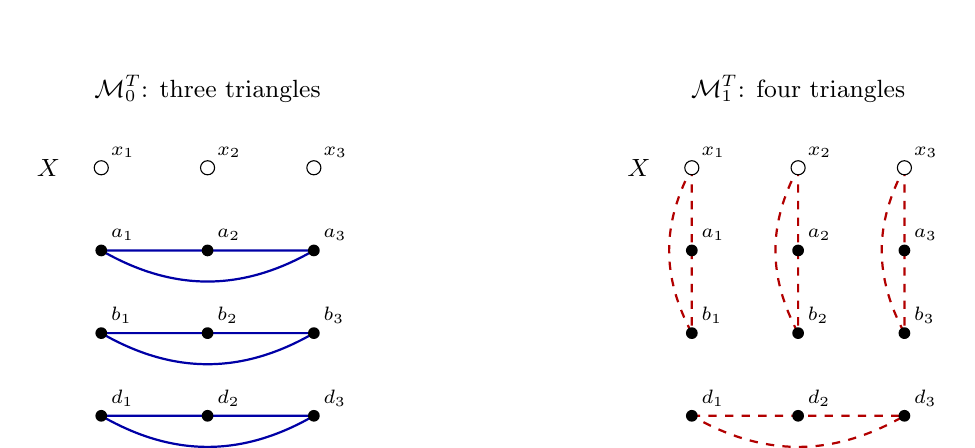
\begin{tikzpicture}[x=1cm,y=1cm,font=\small,>=stealth,
 dot/.style={circle,fill=black,inner sep=1.5pt},
 first/.style={blue!65!black,thick},
 second/.style={red!70!black,thick,dashed},
 shared/.style={green!35!black,very thick},
 spoke/.style={black!45,thin},
 tag/.style={fill=white,inner sep=1pt,font=\scriptsize}]
\begin{scope}[shift={(0,0)}]
\coordinate (p00) at (0.0,0);
\coordinate (p01) at (1.35,0);
\coordinate (p02) at (2.7,0);
\coordinate (p10) at (0.0,-1.05);
\coordinate (p11) at (1.35,-1.05);
\coordinate (p12) at (2.7,-1.05);
\coordinate (p20) at (0.0,-2.1);
\coordinate (p21) at (1.35,-2.1);
\coordinate (p22) at (2.7,-2.1);
\coordinate (p30) at (0.0,-3.15);
\coordinate (p31) at (1.35,-3.15);
\coordinate (p32) at (2.7,-3.15);
\draw[first] (p10)--(p11)--(p12) to[bend left=30] (p10);
\draw[first] (p20)--(p21)--(p22) to[bend left=30] (p20);
\draw[first] (p30)--(p31)--(p32) to[bend left=30] (p30);
\node[circle,draw,fill=white,inner sep=1.8pt] at (p00) {};\node[font=\scriptsize,above right] at (p00) {$ x_1 $};
\node[circle,draw,fill=white,inner sep=1.8pt] at (p01) {};\node[font=\scriptsize,above right] at (p01) {$ x_2 $};
\node[circle,draw,fill=white,inner sep=1.8pt] at (p02) {};\node[font=\scriptsize,above right] at (p02) {$ x_3 $};
\node[dot] at (p10) {};\node[font=\scriptsize,above right] at (p10) {$ a_1 $};
\node[dot] at (p11) {};\node[font=\scriptsize,above right] at (p11) {$ a_2 $};
\node[dot] at (p12) {};\node[font=\scriptsize,above right] at (p12) {$ a_3 $};
\node[dot] at (p20) {};\node[font=\scriptsize,above right] at (p20) {$ b_1 $};
\node[dot] at (p21) {};\node[font=\scriptsize,above right] at (p21) {$ b_2 $};
\node[dot] at (p22) {};\node[font=\scriptsize,above right] at (p22) {$ b_3 $};
\node[dot] at (p30) {};\node[font=\scriptsize,above right] at (p30) {$ d_1 $};
\node[dot] at (p31) {};\node[font=\scriptsize,above right] at (p31) {$ d_2 $};
\node[dot] at (p32) {};\node[font=\scriptsize,above right] at (p32) {$ d_3 $};
\node[anchor=east] at (-.4,0) {$X$};
\node at (1.35,1) {$\mathcal M_0^T$: three triangles};
\end{scope}
\begin{scope}[shift={(7.5,0)}]
\coordinate (p00) at (0.0,0);
\coordinate (p01) at (1.35,0);
\coordinate (p02) at (2.7,0);
\coordinate (p10) at (0.0,-1.05);
\coordinate (p11) at (1.35,-1.05);
\coordinate (p12) at (2.7,-1.05);
\coordinate (p20) at (0.0,-2.1);
\coordinate (p21) at (1.35,-2.1);
\coordinate (p22) at (2.7,-2.1);
\coordinate (p30) at (0.0,-3.15);
\coordinate (p31) at (1.35,-3.15);
\coordinate (p32) at (2.7,-3.15);
\draw[second] (p00)--(p10)--(p20) to[bend left=28] (p00);
\draw[second] (p01)--(p11)--(p21) to[bend left=28] (p01);
\draw[second] (p02)--(p12)--(p22) to[bend left=28] (p02);
\draw[second] (p30)--(p31)--(p32) to[bend left=30] (p30);
\node[circle,draw,fill=white,inner sep=1.8pt] at (p00) {};\node[font=\scriptsize,above right] at (p00) {$ x_1 $};
\node[circle,draw,fill=white,inner sep=1.8pt] at (p01) {};\node[font=\scriptsize,above right] at (p01) {$ x_2 $};
\node[circle,draw,fill=white,inner sep=1.8pt] at (p02) {};\node[font=\scriptsize,above right] at (p02) {$ x_3 $};
\node[dot] at (p10) {};\node[font=\scriptsize,above right] at (p10) {$ a_1 $};
\node[dot] at (p11) {};\node[font=\scriptsize,above right] at (p11) {$ a_2 $};
\node[dot] at (p12) {};\node[font=\scriptsize,above right] at (p12) {$ a_3 $};
\node[dot] at (p20) {};\node[font=\scriptsize,above right] at (p20) {$ b_1 $};
\node[dot] at (p21) {};\node[font=\scriptsize,above right] at (p21) {$ b_2 $};
\node[dot] at (p22) {};\node[font=\scriptsize,above right] at (p22) {$ b_3 $};
\node[dot] at (p30) {};\node[font=\scriptsize,above right] at (p30) {$ d_1 $};
\node[dot] at (p31) {};\node[font=\scriptsize,above right] at (p31) {$ d_2 $};
\node[dot] at (p32) {};\node[font=\scriptsize,above right] at (p32) {$ d_3 $};
\node[anchor=east] at (-.4,0) {$X$};
\node at (1.35,1) {$\mathcal M_1^T$: four triangles};
\end{scope}

\end{tikzpicture}
\caption{A one-class absorber template for $c=3$.
The left factor covers the nine additional vertices; the right factor
covers those vertices together with $X=\{x_1,x_2,x_3\}$.
Every triangle on the right contains at most one root.}
\label{fig:factors:vertex-absorber-template}
\end{figure}


\paragraph{Labeled absorber embeddings.}
Let\phantomsection\label{gls:labeled-embeddings-of-absorber-templates} $V_1,\ldots,V_s$ be disjoint finite sets, and let $\mathcal C$
be a finite indexed family of cycles on their union, each meeting
$V_i$ in $a_i$ vertices. Let $\mathcal T$ be a finite family of
absorber templates with these class sizes. Let $\mathbf a:=(a_1,\ldots,a_s)$ and
\begin{equation*}
 \mathcal R_{\mathbf a}:=\{X\subseteq\textstyle\bigcup_iV_i:
                    |X\cap V_i|=a_i\ (i\in[s])\},\qquad
 \mathcal C_{=X}:=\{C\in\mathcal C:V(C)=X\}.
\end{equation*}
For $X\in\mathcal R_{\mathbf a}$, let
$\mathcal A_{\mathcal C}^{\mathcal T}(X)$ consist of tuples
$(T,\varphi,(C_{j,D})_{j\in\{0,1\},\,D\in\mathcal M_j^T})$ with
$T\in\mathcal T$ and
\begin{equation*}
 \varphi:[h+c]\hookrightarrow\bigcup_iV_i,\qquad \varphi(R_T)=X,
 \qquad \varphi(v)\in V_{\kappa_T(v)}\quad(v\in[h+c]),
\end{equation*}
where, for $j\in\{0,1\}$ and $D\in\mathcal M_j^T$,
\begin{equation*}
 C_{j,D}\in\mathcal C,\qquad
 V(C_{j,D})=\varphi(V(D)),\qquad E(C_{j,D})=\varphi(E(D)).
\end{equation*}
The edge equality preserves all prescribed directions and types.
If $D\in\mathcal M_0^T\cap\mathcal M_1^T$, the pairs $(0,D)$ and $(1,D)$
are distinct indices, although $C_{0,D}$ and $C_{1,D}$ may be the same
member of $\mathcal C$.
The count retains $T$, the full map $\varphi$, and every cycle identifier.
A factor on $S$ is a subfamily $\mathcal F\subseteq\mathcal C$ with
$S=\mathop{\dot\bigcup}_{C\in\mathcal F}V(C)$. Thus the two indexed
cycle families in an absorber are factors on $\varphi([h])$ and
$\varphi([h])\dot\cup X$. These definitions impose no proportionality
condition on the sizes of the $V_i$. A multiplicity bound
$|\mathcal C_{=X}|\le J$ is imposed only when stated.

\paragraph{One-class templates and ordered roots.}\label{gls:labeled-embeddings-of-absorber-templates:ordered-roots}
For untyped undirected $c$-cycles, let $\mathfrak T_c$ be the family
of all one-class absorber templates with class size $c$. Their class
map is the constant map to $1$. For an ordering
$\mathbf x=(x_1,\ldots,x_c)$ of $X$, let
\begin{equation*}
 \mathcal A_{\mathcal C}^{\mathcal T}(\mathbf x)
 :=\{(T,\varphi,(C_{j,D}))\in\mathcal A_{\mathcal C}^{\mathcal T}(X):
                         \varphi(h+i)=x_i\ (i\in[c])\}.
\end{equation*}
For directed or typed cycles, the templates have the specified
directions and types, and their labeled embeddings are defined in the same way.


\Needspace{8\baselineskip}
\begin{definition}[Cycle weight and absorber estimates]\label{gls:cycle-weight-and-absorber-estimates}
\label{def:cycle:weight-absorber-estimates}
Let $V_1,\ldots,V_s$ be disjoint finite sets, let $a_1,\ldots,a_s$
be positive integers with $c:=\sum_i a_i\ge3$, and let $\mathcal C$
be a finite indexed family of $c$-cycles on $\bigcup_iV_i$, each meeting $V_i$ in $a_i$ vertices.
Let $\mathbf a:=(a_1,\ldots,a_s)$ and let $\mathcal T$ be a fixed finite family
of absorber templates with these class sizes. Let $m,a_{\rm abs}>0$, $B_{\omega}>1$ and $\eta\ge0$.
A weighting $\phi:\mathcal C\to\mathbb R_{\ge0}$ has
\emph{cycle weight and absorber estimates at scale $m$}, with
error $\eta$, coefficient bound $B_{\omega}$ and absorber coefficient
$a_{\rm abs}$, for $\mathcal T$, if
\begin{align*}
B_{\omega}^{-1}m^{1-c}\le\phi(C)&\le B_{\omega}m^{1-c} &&(C\in\mathcal C),
 \\
 \sum_{C\in\mathcal C:v\in V(C)}\phi(C)&=1\pm \eta
 &&(v\in\textstyle\bigcup_iV_i),
 \\
 |\mathcal A_{\mathcal C}^{\mathcal T}(X)|&\ge a_{\rm abs}m^{c^2}
 &&(X\in\mathcal R_{\mathbf a}).
\end{align*}
\end{definition}

If $0<\lambda_0\le1$ and $\lambda_0m\le k\le m$, the three
inequalities in Definition~\ref{def:cycle:weight-absorber-estimates}
also hold at scale $k$, with coefficient bound
$B_{\omega}\lambda_0^{1-c}$ and with the same vertex-sum error
and absorber-count coefficient. Indeed
$m^{1-c}\ge\lambda_0^{c-1}k^{1-c}$, $m^{1-c}\le k^{1-c}$ and
$m^{c^2}\ge k^{c^2}$. Exact class-size ratios are imposed separately
in the results below.

\Needspace{8\baselineskip}
\begin{lemma}
\label{lem:simp:profile-marginals}
Let $s\ge1$ and $a_1,\ldots,a_s$ be positive integers, let $c:=\sum_i a_i\ge3$,
and let $J\ge1$. Let $\mathcal T$ be a fixed finite family of absorber templates
with class sizes $(a_1,\ldots,a_s)$.
Let $a>0$ and $B>1$. There are $\eta_0>0$ and $k_0>1$ such that
the following holds for every real $k\ge k_0$ with all $a_i k$ integral.
Let $V_1,\ldots,V_s$ be disjoint sets with $|V_i|=a_i k$, and let
$\mathcal C$ be a finite indexed family of cycles with
$|V(C)\cap V_i|=a_i$ for every $C\in\mathcal C$ and $i\in[s]$.
Assume that $|\{C\in\mathcal C:V(C)=X\}|\le J$
for every $X\in\binom{\bigcup_iV_i}{c}$.
Let $0\le\eta\le\eta_0$ and let $\phi$ have cycle weight and absorber
estimates at scale $k$, with error $\eta$, coefficient bound $B$
and absorber coefficient $a$, for $\mathcal T$.
Then there is $\psi:\mathcal C\to\mathbb R_{\ge0}$ satisfying
\begin{equation*}
 \sum_{C\in\mathcal C:v\in V(C)}\psi(C)=1\quad(v\in\bigcup_iV_i),\qquad
 \frac{k^{1-c}}{2B}\le\psi(C)\le2Bk^{1-c}
       \quad(C\in\mathcal C).
\end{equation*}
\end{lemma}

\Needspace{8\baselineskip}
\begin{lemma}[Cycle factors with prescribed class sizes]
\label{lem:simp:profile-factor}
Let $s\ge1$ and $a_1,\ldots,a_s$ be positive integers, let $c:=\sum_i a_i\ge3$,
and let $J\ge1$. Let $\mathcal T$ be a fixed finite family of absorber templates
with class sizes $(a_1,\ldots,a_s)$.
Let $a>0$ and $B>1$. There exist $\eta_*>0$ and an integer $k_0$
such that the following holds for every integer $k\ge k_0$.
Let $V_1,\ldots,V_s$ be disjoint sets with $|V_i|=a_i k$, and let
$\mathcal C$ be a finite indexed family of cycles with
$|V(C)\cap V_i|=a_i$ for every $C\in\mathcal C$ and $i\in[s]$.
Assume that $|\{C\in\mathcal C:V(C)=X\}|\le J$
for every $X\in\binom{\bigcup_iV_i}{c}$.
Let $\phi$ have cycle weight and absorber estimates at scale $k$,
with error $\eta_*$, coefficient bound $B$ and absorber
coefficient $a$, for $\mathcal T$.
Then there is a factor $\mathcal F\subseteq\mathcal C$
on $\bigcup_iV_i$.
\end{lemma}

\begin{proof}[Proof of Lemma~\ref{lem:simp:profile-marginals}]
Let $h:=c^2$.
For $X\in\mathcal R_{\mathbf a}$ and
$\alpha=(T,\varphi,(C_{j,D}))\in\mathcal A_{\mathcal C}^{\mathcal T}(X)$,
write $\mathcal M_j(\alpha):=\{C_{j,D}:D\in\mathcal M_j^T\}$ for its
two indexed cycle factors. Define
\begin{equation*}
 T_X(C):=\frac{1}{|\mathcal A_{\mathcal C}^{\mathcal T}(X)|}
 \sum_{\alpha\in\mathcal A_{\mathcal C}^{\mathcal T}(X)}
 \left(\mathbf1_{\{C\in\mathcal M_1(\alpha)\}}
       -\mathbf1_{\{C\in\mathcal M_0(\alpha)\}}\right).
\end{equation*}
Each free vertex occurs once in each of $\mathcal M_0(\alpha)$ and
$\mathcal M_1(\alpha)$, whereas each root occurs only in
$\mathcal M_1(\alpha)$, so
\begin{equation}
 \sum_{C\ni v}T_X(C)=\ind_{\{v\in X\}}.
 \label{eq:repair:trade-incidence}
\end{equation}
For a fixed template and cycle position, a cycle $C$ disjoint
from $X$ fixes $c$ free labels, leaving $O(k^{h-c})$ labeled absorbers.
A contributing cycle meeting $X$ belongs to $\mathcal M_1(\alpha)$
and meets $X$ once. It fixes $c-1$ free labels, leaving
$O(k^{h-c+1})$ labeled absorbers. A cycle meeting $X$ twice
or more cannot contribute. There are only boundedly many templates,
cycle positions and cycle identifiers on each chosen vertex set.
Dividing these counts by
$|\mathcal A_{\mathcal C}^{\mathcal T}(X)|\ge ak^h$ gives
\begin{equation}
 |T_X(C)|\le K\bigl(k^{-c}
       +\ind_{\{V(C)\cap X\ne\varnothing\}}k^{1-c}\bigr).
 \label{eq:repair:trade-spread}
\end{equation}
Here, and below the counting constants depend only on
$s,(a_i)_{i\in[s]},J,\mathcal T,a,B$.

Write $z_v:=1-\sum_{C\ni v}\phi(C)$ and $n_i:=a_i k$.
Since each cycle uses $a_i$ vertices in class $i$, $\sum_{v\in V_i}z_v=a_i\left(k-\sum_C\phi(C)\right)$. Thus
$\mu:=n_i^{-1}\sum_{v\in V_i}z_v$ is independent of $i$,
and $|\mu|\le\eta$. Put $y_v:=z_v-\mu$, so its sum in each class
is zero. Let $M:=|\mathcal R_{\mathbf a}|=\prod_i\binom{n_i}{a_i}$.
We seek coefficients $t_X$, $X\in\mathcal R_{\mathbf a}$, such that
$\sum_{X\ni v}t_X=z_v$ for every $v$.
Then adding $\sum_X t_XT_X$ to $\phi$ corrects every vertex sum,
by \eqref{eq:repair:trade-incidence}.
We define
\begin{equation*}
t_X:=\frac1M\left(k\mu+
   \sum_{i=1}^s\frac{n_i(n_i-1)}{a_i(n_i-a_i)}
                      \sum_{v\in X\cap V_i}y_v\right).
\end{equation*}
Let $X_i$ be independent uniform $a_i$-subsets of $V_i$.
Then $X:=\bigcup_iX_i$ is uniform on $\mathcal R_{\mathbf a}$. For $v\in V_i$,
\begin{equation*}
 \Pr(v\in X_i)=\frac1k,\qquad
 \mathbb E\left[\ind_{\{v\in X_i\}}\sum_{u\in X_i}y_u\right]
   =\frac{a_i(n_i-a_i)}{n_i(n_i-1)}y_v.
\end{equation*}
The second identity follows by separating $u=v$ and using
$\sum_{u\ne v}y_u=-y_v$. For $\ell\ne i$, independence and $\sum_{u\in V_\ell}y_u=0$ give
$\mathbb E[\mathbf1_{\{v\in X_i\}}\sum_{u\in X_\ell}y_u]=0$.
Consequently
$\sum_{X\ni v}t_X=\mu+y_v=z_v$.
Also $M=\Theta(k^c)$ and $|t_X|\le K_1\eta k^{1-c}$.

It follows that the weighting $\psi$ defined by
$\psi(C):=\phi(C)+\sum_Xt_XT_X(C)$ has vertex sum one at every vertex.
There are $O(k^c)$ root sets altogether and $O(k^{c-1})$ meeting
a fixed cycle. Equation~\eqref{eq:repair:trade-spread} therefore yields
$|\psi(C)-\phi(C)|\le K_2\eta k^{1-c}$.
Taking $\eta_0\le 1/(2BK_2)$ proves both coefficient bounds.
\end{proof}

\begin{proof}[Proof of Lemma~\ref{lem:simp:profile-factor}]
Let $h:=c^2$.
Let $\eta_{\rm cor},k_{\rm cor}$ be supplied by
Lemma~\ref{lem:simp:profile-marginals} with
$(a/2,2^{c-1}B)$ playing the roles of $(a,B)$.
For every $X\in\mathcal R_{\mathbf a}$ and every $v\notin X$,
at most $C_{\rm abs}k^{h-1}$ members of
$\mathcal A_{\mathcal C}^{\mathcal T}(X)$ have $v$ as a free label.
Also, for distinct $v,w$, the bound of $J$ cycles on each vertex set gives
$\sum_{C:v,w\in V(C)}\phi(C)\le C_{\rm deg}/k$.

For a labeled absorber $\alpha=(T,\varphi,(C_{j,D}))$, let
\begin{equation*}
 f(\alpha):=\left((\varphi(1),\ldots,\varphi(h)),
                  \{C_{0,D}:D\in\mathcal M_0^T\}\right).
\end{equation*}
Thus $f(\alpha)$ records an ordering of the free vertices and
the cycle identifiers of a specified factor on those vertices.
Let $\mathcal D_X:=\{f(\alpha):\alpha\in\mathcal A_{\mathcal C}^{\mathcal T}(X)\}$
and $\mathcal D:=\bigcup_{X\in\mathcal R_{\mathbf a}}\mathcal D_X$.
For every member of $\mathcal D_X$, both the set of its free labels
and the union of that set with $X$ admit factors in $\mathcal C$.
There are constants $K,K',a'>0$ such that
$|\mathcal D|\le Kk^h$, at most $K'k^{2h-1}$ pairs of distinct
members have intersecting free sets, and $|\mathcal D_X|\ge a'k^h$.
Indeed, fixing the ordered free labels leaves boundedly many internal
factors, and an intersecting pair identifies a free label in each tuple.
For fixed $X$ and $f(\alpha)$, there are boundedly many choices for
$T$, the root ordering and the remaining cycle identifiers.
For fixed $s,(a_i),J,\mathcal T$, the counting bounds and the
application of Lemma~\ref{lem:simp:profile-marginals} use only
a positive lower bound on $a$ and an upper bound on $B$.
We choose
\begin{equation*}
 0<1/k_0\ll\gamma\ll\rho\ll\delta\ll\eta_*
 \ll\eta_{\rm cor},a,a',1/C_{\rm abs},1/C_{\rm deg},1/K,1/K',1/h,1/B,1/J,1/c,
\end{equation*}
with $k_0\ge2k_{\rm cor}$.

We first construct $A_0$ with $|A_0|\le\delta k$ and
$|A_0\cap V_i|=a_iq_0$ for an integer $q_0\ge0$, such that
$A_0\cup W$ has a factor for every
$W\subseteq(\bigcup_iV_i)\setminus A_0$ satisfying
$|W|\le\gamma k$ and $|W\cap V_i|=a_iq$ for an integer $q\ge0$.
We adapt the random-selection argument of
Lo--Markstr\"om~\cite[proof of Lemma~1.1]{LoMarkstrom2015}
to obtain members of $\mathcal D$ with pairwise disjoint sets of free labels.
Let $\mathcal D^*$ be the random subfamily obtained by selecting each
member of $\mathcal D$ independently with probability $\rho k^{1-h}$.
Chernoff's inequality (Lemma~\ref{lem:prelim:chernoff})
and a union bound over the $O(k^c)$ root sets show that, with
probability tending to one, at most $2K\rho k$ members of $\mathcal D$
are selected and at least $a'\rho k/2$ belong to each $\mathcal D_X$.
The expected number of selected pairs with intersecting free sets
is at most $K'\rho^2k$. Markov's inequality and the preceding
probability estimate give an outcome satisfying both conclusions
and having at most $2K'\rho^2k$ such pairs.

For this outcome, let $\mathcal D_0$ consist of the members of
$\mathcal D^*$ whose free sets are disjoint from those of every other
member of $\mathcal D^*$. At most $4K'\rho^2k$ members are removed.
Since $4K'\rho\le a'/4$,
we have $|\mathcal D_0\cap\mathcal D_X|\ge a'\rho k/4$ for every $X$.
Let $A_0$ be the union of the pairwise disjoint free sets of the members
of $\mathcal D_0$. Each free set has $ca_i$ vertices in $V_i$, so
$q_0=c|\mathcal D_0|$ and $|A_0|\le2hK\rho k\le\delta k$.
For a set $W$ as above, the class-size identities give a partition
of $W$ into $q$ members of $\mathcal R_{\mathbf a}$.
After assigning members of $\mathcal D_0$ to $t<q$ of them, the next root set
has at least $a'\rho k/4-t>0$ unused choices, since
$q\le|W|\le\gamma k<a'\rho k/4$.
For each assigned member, we use a factor on the union of its
set of free labels and its assigned root set. For each remaining member
of $\mathcal D_0$, we use its recorded factor. Their union is a
factor on $A_0\cup W$.
Taking $W=\varnothing$ gives a factor on $A_0$.

Put $V_i':=V_i\setminus A_0$ and
$\mathcal C':=\{C\in\mathcal C:V(C)\cap A_0=\varnothing\}$.
For every $X\in\mathcal R_{\mathbf a}$ disjoint from $A_0$,
\begin{equation*}
 |\mathcal A_{\mathcal C'}^{\mathcal T}(X)|
 \ge(a-C_{\rm abs}\delta)k^h\ge(a/2)k^h.
\end{equation*}
For every $v\notin A_0$, the loss of vertex weight is at most
\begin{equation*}
 \sum_{x\in A_0}\sum_{C:v,x\in V(C)}\phi(C)
 \le |A_0|C_{\rm deg}/k\le C_{\rm deg}\delta.
\end{equation*}
The classes $V_i'$ have sizes $a_i k'$, where $k':=k-q_0$ is
an integer and $k/2\le k'\le k$. Thus
$\phi|_{\mathcal C'}$ has coefficient bound
$2^{c-1}B$ at scale $k'$, absorber coefficient $a/2$, and
vertex-sum error at most $\eta_*+C_{\rm deg}\delta\le\eta_{\rm cor}/2$.
Since $k'\ge k/2\ge k_{\rm cor}$,
Lemma~\ref{lem:simp:profile-marginals} gives a weighting $\psi$ on
$\mathcal C'$ with vertex sums exactly one and
$\psi(C)\le2^cB(k')^{1-c}$.

Let $\mathcal H$ have vertex set $\bigcup_iV_i'$, indexed edge set
$\mathcal C'$ and incidence map $C\mapsto V(C)$, with weights $\psi(C)$.
For distinct $v,w\in V(\mathcal H)$,
\begin{equation*}
 d_\psi^{\mathcal H}(v,w)
 \le J\binom{ck'-2}{c-2}2^cB(k')^{1-c}
 \le K_{\rm cd}/k',
\end{equation*}
where $K_{\rm cd}$ depends only on $c,J,B$.
We apply Lemma~\ref{lem:new:weighted-resource-matching} with
rank $r=c$, weighting $w=\psi$, no additional weight functions,
and the following parameters:
\begin{equation*}
\begin{array}{c|cccccc}
\text{parameter}&n&B&K&a&\mathcal S&\gamma\\\hline
\text{value}&k'&2&K_{\rm cd}&1&\{V(\mathcal H)\}&\min\{1/2,\gamma/(2c)\}.
\end{array}
\end{equation*}
Here, $k_0$ is sufficiently large that $k'\ge k/2$ exceeds the
order threshold in that lemma and $k'\ge c$.
Then $k'\le|V(\mathcal H)|=ck'\le(k')^2$.
Since the vertex sums of $\psi$ are exactly one, they satisfy
the load condition for the tolerance supplied by that lemma.
Let $M$ be the resulting matching and $W$ its uncovered set. Then
$W$ has at most
$\min\{1/2,\gamma/(2c)\}ck'\le\gamma k/2$ vertices.
Every selected cycle uses $a_i$ vertices of $V_i'$, so
$|W\cap V_i'|=a_iq$ for the nonnegative integer $q:=k'-|M|$.
The factor on $A_0\cup W$ constructed
above, together with $M$, is the required factor.
\end{proof}

\Needspace{6\baselineskip}
\subsection{Paired absorbers and factor applications}

Let\phantomsection\label{gls:paired-cycle-factor-absorbers} $c\ge3$ be an integer, let $V$ be finite, and let $\mathcal C$ be an indexed
family of cycles on $V$, each with $c$ distinct vertices. Let
$\mathcal C_{=Z}:=\{C\in\mathcal C:V(C)=Z\}$.
For $X\in\binom Vc$, let $\mathcal A_{\mathcal C}^{\rm pair}(X)$ consist of
all the following labeled tuples: an ordering $(x_0,\ldots,x_{c-1})$ of $X$,
an ordered tuple $(y_0,\ldots,y_{c-1})$, ordered tuples
$(p_{i,1},\ldots,p_{i,c-1})$ for $0\le i<c$, and cycle identifiers
\begin{equation}
 C_*\in\mathcal C_{=Y},\quad
 C_i^0\in\mathcal C_{=P_i\cup\{y_i\}},\quad
 C_i^1\in\mathcal C_{=P_i\cup\{x_i\}}\quad(0\le i<c),
\label{eq:cycle:paired-absorbers}
\end{equation}
where $Y:=\{y_0,\ldots,y_{c-1}\}$ and $P_i:=\{p_{i,1},\ldots,p_{i,c-1}\}$.
All free labels are distinct and outside $X$. Their set
$S:=Y\dot\cup\mathop{\dot\bigcup}_{i=0}^{c-1}P_i$ has size $c^2$.
The two cycle subfamilies
$\mathcal M_0:=\{C_i^0:0\le i<c\}$ and
$\mathcal M_1:=\{C_*\}\cup\{C_i^1:0\le i<c\}$ are factors on $S$ and $S\cup X$.
Every ordering and cycle identifier is included in this indexed count.
Class restrictions on $x_i,y_i,p_{i,j}$ are imposed separately when this family is used.
These tuples correspond to template embeddings with positions given by
\begin{equation*}
 \varphi(h+i+1)=x_i,\qquad \varphi(i+1)=y_i,\qquad
 \varphi(c+i(c-1)+j)=p_{i,j}
 \quad(0\le i<c,\ 1\le j<c),
\end{equation*}
where $h:=c^2$. Pulling the two factors back along $\varphi$ gives
a template, with the prescribed classes, directions and types.
The resulting labeled embedding recovers every ordered label and
cycle identifier, so this map is injective. For fixed class and type
restrictions, the possible position templates form a fixed finite
family. Its absorber count is at least the paired count.
No paired form is required of a general template. The definition
\eqref{eq:cycle:paired-absorbers} does not require $C_i^0$ and $C_i^1$
to induce the same path on $P_i$.


Let\phantomsection\label{gls:paired-cycle-factor-absorbers:two-class} $r\ge2$ be an integer, let $c:=r+1$ and $h:=c^2$, and let $A,B$
be disjoint finite sets. Let $\mathcal C$ be an indexed family of
undirected or directed $c$-cycles, with any specified edge types,
each having one vertex in $A$ and $r$ in $B$. Let
\begin{equation}
\mathcal R_r(A,B):=\{X\subseteq A\cup B:|X\cap A|=1,\ |X\cap B|=r\},
\qquad \mathcal C_{=X}:=\{C\in\mathcal C:V(C)=X\}.
\label{eq:roots:two-classes}
\end{equation}
For $X\in\mathcal R_r(A,B)$, define the restricted paired-absorber family by
\begin{equation}
 \mathcal A_{\mathcal C}(X)
 :=\{\alpha\in\mathcal A_{\mathcal C}^{\rm pair}(X):
       x_0,y_0\in A,\ x_i,y_i\in B\ (1\le i\le r)\},
 \label{eq:paired-absorbers:two-classes}
\end{equation}
where $(x_0,\ldots,x_r)$ and $(y_0,\ldots,y_r)$ are the root and
base orderings of $\alpha$. All admissible orderings and cycle
identifiers are counted. Each absorber has $h$ free vertices,
$c$ in $A$ and $rc$ in $B$, and factors $\mathcal M_0,\mathcal M_1$
of its free set and of that set together with $X$, respectively.

We\phantomsection\label{gls:cycle-weight-and-absorber-estimates:paired} use \emph{cycle weight and absorber estimates with paired absorbers}
for the same three inequalities in
Definition~\ref{def:cycle:weight-absorber-estimates}, with vertex classes
$(A,B)$, multiplicities $(1,c-1)$, root family $\mathcal R_{c-1}(A,B)$,
and the count $|\mathcal A_{\mathcal C}(X)|$ in the last inequality.
The injection above verifies the template-embedding lower bound
required by Lemma~\ref{lem:simp:profile-factor} and
Theorem~\ref{thm:simp:profile-finite-cleanup}.

\paragraph{Extracting factors from cycle weights.}
Lemma~\ref{lem:simp:profile-factor} applies to a prescribed family
of cycles, including families
obtained after sampling vertices or imposing further restrictions.

For a family $\mathcal C\subseteq\mathcal C_r(Q)$ on an $m$-vertex
graph with $r\mid m$, we apply Lemma~\ref{lem:simp:profile-factor} with
$s=1$, $a_1=r$ and $k=m/r$. The lower bounds
$|\mathcal A_{\mathcal C}^{\mathfrak T_r}(X)|\ge am^{r^2}$ for
$X\in\binom{V(Q)}r$, and the coefficient bounds
$B^{-1}m^{1-r}\le\phi(C)\le Bm^{1-r}$ imply, at scale $k$, the bounds
\begin{equation}
 ar^{r^2}k^{r^2},\qquad
 \frac{k^{1-r}}{Br^{r-1}}\le\phi(C)\le Br^{r-1}k^{1-r}.
 \label{eq:factor:single-class-scaling}
\end{equation}
With the vertex-sum error supplied by that lemma, it gives a factor
in $\mathcal C$. Both factors in each absorber must lie in $\mathcal C$.


\Needspace{8\baselineskip}
\section{Two cycle factors on a bounded extension}

Under the hypotheses of Theorem~\ref{thm:simp:profile-finite-cleanup},
a bounded prescribed set $Z$ can be augmented by a bounded set $S$
disjoint from $Z$, such that both $S$ and $S\cup Z$ admit cycle factors.
The underlying auxiliary edge sets of the two factors are disjoint.
These factors are used in the transformer constructions in
Sections~\ref{sec:new:ordinary-relative-absorber}
and~\ref{sec:four:marked-absorber}.

Directed cycles and cycles with prescribed edge types are allowed.
Distinct cycle identifiers with the same vertex set are counted
separately in the multiplicity bound $J$.
For a cycle or factor $D$, let
\begin{equation*}
 E_{\rm aux}(D):=\{\{x,y\}:\text{$D$ has an edge or arc with endpoints $x,y$}\}.
\end{equation*}
Thus $E_{\rm aux}(D)$ records auxiliary endpoints, without directions
or types.

\begin{theorem}[Two cycle factors on a bounded extension]
\label{thm:simp:profile-finite-cleanup}
Let $s\ge1$ and $a_1,\ldots,a_s$ be positive integers, let $c:=\sum_i a_i\ge3$,
and let $J\ge1$. Let $\mathcal T$ be a fixed finite family of absorber templates
with class sizes $(a_1,\ldots,a_s)$.
Let
$a>0$ and $B>1$. There exists $\eta>0$ such that, for every integer
$q\ge0$, there is an integer $t\ge1$ such that, for every
$F_0,\Delta_{\rm forb}\ge0$, there is $k_0>1$ with the following property.

Let $k\ge k_0$ be real with all $a_i k$ integral, and let
$V_1,\ldots,V_s$ be disjoint sets with $|V_i|=a_i k$. Let
$\mathcal C$ be a finite indexed family of cycles with
$|V(C)\cap V_i|=a_i$ for every $C\in\mathcal C$ and $i\in[s]$,
and $|\{C\in\mathcal C:V(C)=X\}|\le J$
for every $X\in\binom{\bigcup_iV_i}{c}$. Let
$\phi:\mathcal C\to\mathbb R_{\ge0}$, let
$T\subseteq\bigcup_iV_i$ have $|T|\le F_0$, and let $J_0$
be a simple graph on $\bigcup_iV_i$ with $\Delta(J_0)\le \Delta_{\rm forb}$.

Suppose $\phi$ has cycle weight and absorber estimates at scale $k$,
with error $\eta$, coefficient bound $B$ and absorber coefficient
$a$, for $\mathcal T$.

Let $Z\subseteq\bigcup_iV_i$ satisfy $|Z\cap V_i|=a_i z$
for every $i\in[s]$, where $z$ is an integer with $0\le z\le q$.
Then there exist $S\subseteq(\bigcup_iV_i)\setminus(Z\cup T)$ and
factors $D^0,D^1\subseteq\mathcal C$ on $S,S\cup Z$, respectively,
with $E_{\rm aux}(D^0)\cap E_{\rm aux}(D^1)=\varnothing$, such that
\begin{equation*}
 |S\cap V_i|=a_it\quad(i\in[s]),\qquad E(J_0[S])=\varnothing,
 \qquad |V(C)\cap Z|\le1\quad(C\in D^1).
\end{equation*}
\end{theorem}
\begin{proof}
Let $h:=c^2$.
Let $\eta_{\rm fac}>0$ and $k_{\rm fac}$ be supplied by
Lemma~\ref{lem:simp:profile-factor} with
$(a_{\rm fac},B_{\rm fac})=(a/2^{h+3},2^{c-1}B)$.
Before $q$ is given, choose
\begin{equation*}
 0<\eta\ll\xi\ll\eta_{\rm fac},a_{\rm fac},1/B_{\rm fac},a,1/B,1/J,1/c.
\end{equation*}
We take an integer $t\ge\max\{q,k_{\rm fac}\}$ sufficiently large
after $q,\xi$, and then $k$ sufficiently large after $t,F_0,\Delta_{\rm forb}$.
All counting constants below depend only on
$s,(a_i)_{i\in[s]},J,\mathcal T,a,B$.

\emph{The sample $S$.}
Independently for each $i$, let $(v_{i,1},\ldots,v_{i,a_it})$ be a uniformly
chosen ordered tuple of distinct vertices of $V_i\setminus(Z\cup T)$.
Put $S_i:=\{v_{i,1},\ldots,v_{i,a_it}\}$ and $S:=\bigcup_iS_i$.
For $\phi_t:=(k/t)^{c-1}\phi$ and $v\in S\cup Z$, write
\begin{equation*}
 \Phi(v):=\sum_{\substack{C\in\mathcal C:\ v\in V(C)\\
                         V(C)\setminus\{v\}\subseteq S}}\phi_t(C).
\end{equation*}
For $v\in Z$ we leave the samples unconditioned. For a sample
position we condition on its label $v$. Conditional on this label,
the remaining sets are independent uniform subsets of the remaining
populations. All expectations and probabilities in the following
calculation are taken under the corresponding distribution.
Cycles through $v$ and another vertex of $Z\cup T$ have total
original weight $O((q+F_0)/k)$, since two prescribed labels lie
in $O(k^{c-2})$ cycles. For each remaining cycle, the probability
that its other $c-1$ labels lie in $S$ is
$(t/k)^{c-1}(1+O(1/t)+O_{q,F_0}(1/k))$.
This follows by multiplying the classwise falling-factorial ratios,
subtracting one from the sample and population sizes in the class
of a conditioned sample position. Thus the expected value of $\Phi(v)$ is
\begin{equation}
 1\pm\bigl(\eta+O(1/t)+O_{q,F_0}(1/k)\bigr).
 \label{eq:new:finite-weighted-cleanup:F12}
\end{equation}
Replacing one sampled vertex by an unsampled vertex in the same
class, while keeping $v$ fixed, affects $O(t^{c-2})$ cycles through
$v$. Each has weight at most $Bt^{1-c}$, so the change in $\Phi(v)$
is at most $K_1/t$. This function depends only on the sampled sets,
not on their ordering. We apply the subset case of the sampling
concentration inequality (Lemma~\ref{lem:simp:product-sampling})
to the remaining sets. Their total size is at most $ct$, and an exchange changes
$\Phi(v)$ by at most $K_1/t$. Hence the probability of a deviation
larger than $\xi$ is at most $2\exp(-2\xi^2t/(cK_1^2))$.

For $X\in\mathcal R_{\mathbf a}$ contained in $S\cup Z$, let
$A_X(S)$ count the members of $\mathcal A_{\mathcal C}^{\mathcal T}(X)$
whose free vertices all lie in $S$. We index $X$ by its vertices in
$Z$ and its positions in the ordered samples, and condition on
the labels at those positions. At least
$ak^h-O((q+F_0)k^{h-1})$ members of
$\mathcal A_{\mathcal C}^{\mathcal T}(X)$ have all free labels outside
$Z\cup T$. Each has $ca_i$ free labels in class $i$, so their
inclusion probability is
\begin{equation*}
 \prod_i\frac{(a_it-|X\cap S_i|)_{ca_i}}
                  {(a_ik-|(Z\cup T)\cap V_i|-|X\cap S_i|)_{ca_i}}
 =(t/k)^h\bigl(1+O(1/t)+O_{q,F_0}(1/k)\bigr),
\end{equation*}
where $(x)_j:=x(x-1)\cdots(x-j+1)$. Thus the conditional expectation
of $A_X(S)$ is at least $at^h/2$. An exchange in a remaining sampled
set changes $A_X(S)$ by at most $K_2t^{h-1}$, since each affected
embedding contains an exchanged free vertex. The subset case of the
sampling concentration inequality (Lemma~\ref{lem:simp:product-sampling})
therefore bounds the probability that $A_X(S)<at^h/4$ by
$2\exp(-\kappa_0t)$ for some $\kappa_0>0$.
Averaging these uniform conditional bounds and taking a union bound
over $ct+|Z|$ vertex positions and at most $\binom{ct+|Z|}{c}$
root-position choices gives failure probability less than $1/4$.
Also $\mathbb E e(J_0[S])=O(\Delta_{\rm forb}t^2/k)<1/4$ for large $k$.
Together with \eqref{eq:new:finite-weighted-cleanup:F12},
Markov's inequality and the preceding union bound give an outcome
with $E(J_0[S])=\varnothing$ such that
\begin{equation*}
 \Phi(v)=1\pm (\eta+\xi+O(1/t)+O_{q,F_0}(1/k))
       \quad(v\in S\cup Z),\qquad
 A_X(S)\ge at^h/4
       \quad(X\in\mathcal R_{\mathbf a},\ X\subseteq S\cup Z).
\end{equation*}
We fix such an $S$.

\emph{The factor $D^0$ on $S$.}
Let $\mathcal C^0:=\{C\in\mathcal C:V(C)\subseteq S\}$.
The restriction $\phi_t|_{\mathcal C^0}$ has weights between
$B^{-1}t^{1-c}$ and $Bt^{1-c}$ and vertex sums $\Phi(v)$.
Each $X\in\mathcal R_{\mathbf a}$ contained in $S$ has at least
$at^h/4$ absorbers in $\mathcal C^0$. The displayed bound for
$|\Phi(v)-1|$ is at most $\eta_{\rm fac}$ for large $t,k$.
Lemma~\ref{lem:simp:profile-factor}, with scale $t$ and constants
$(a_{\rm fac},B_{\rm fac})$, gives a factor $D^0$ on $S$.

\emph{The factor $D^1$ on $S\cup Z$.}
Let $\mathcal C^1$ consist of the cycles in $\mathcal C$ on $S\cup Z$
that meet $Z$ at most once and satisfy
$E_{\rm aux}(C)\cap E_{\rm aux}(D^0)=\varnothing$.
For $v\in S$, the cycles through $v$ that meet $Z$ exactly once
have total weight at most $K_3q/t$: prescribing their vertex in $Z$
leaves $O((t+q)^{c-2})$ cycles, each of weight at most $Bt^{1-c}$.
For $v\in Z$, all cycles on $S\cup Z$ through $v$ meeting $Z$
exactly once are already counted by $\Phi(v)$.
Deleting the cycles $C$ with $E_{\rm aux}(C)\cap E_{\rm aux}(D^0)\ne\varnothing$
reduces each vertex sum by at most $K_4/t$. Indeed, at most two edges of $D^0$
meet $v$ and fix one additional label, while each of its other
at most $ct$ edges fixes two. Directions and parallel types do
not affect these bounds, since every edge specifies its endpoints.

For each root set $X\subseteq S\cup Z$, the counted absorbers
have all free labels in $S$, and each cycle of their second factor
contains at most one root. Thus none of their cycles meets $Z$ twice.
At most $2c$ edges of $D^0$ meet $X$, each fixing at least one
free label in an absorber, whereas every other edge fixes two. At most
$K_5t^{h-1}$ absorbers are therefore lost. Taking $K_5/t\le a/8$
leaves at least $at^h/8$ absorbers in $\mathcal C^1$ per root.
At scale $t+z\in[t,2t]$, the required coefficient bounds are
\begin{equation*}
 B^{-1}(t+z)^{1-c}\le\phi_t(C)\le B_{\rm fac}(t+z)^{1-c},\qquad
 at^h/8\ge a_{\rm fac}(t+z)^h.
\end{equation*}
For a fixed $K$ bounding the preceding errors, the vertex-sum
error is at most $\eta+\xi+K(q+1)/t+O_{q,F_0}(1/k)\le\eta_{\rm fac}$.
Lemma~\ref{lem:simp:profile-factor}, with scale $t+z$ and the same
constants, gives $D^1\subseteq\mathcal C^1$, as required.
\end{proof}


\Needspace{8\baselineskip}
\section{Cycle factors after independent vertex sampling}

The next lemma finds cycle factors after independent vertex sampling,
assuming positive cycle weights and suitable absorber counts in the
graph before sampling. This graph is fixed for the sampling experiment,
but may be the outcome of an earlier random or deterministic construction.


\Needspace{8\baselineskip}
In the following lemma, all directions and assigned edge types are
fixed before sampling. For untyped graphs and digraphs, physical
edge sets are the underlying unordered edge sets $E_{\rm phys}(F)$.
In the typed case, let $\pi$ be a fixed permutation of a finite ambient set
containing all auxiliary labels. Physical images are given by \eqref{eq:physical:image-map}.
The sampled subsets need not be $\pi$-invariant.
Whenever the candidates contain type-$K$ arcs, the cycles and
absorber embeddings are physically injective and preserve all
prescribed directions and types.


\begin{lemma}[Cycle factors after independent vertex sampling]
\label{lem:new:bernoulli-factor}
Let $a,J>0$ and $B>1$, and let $c\ge3$ be an integer.
There are $\eta_0,\zeta>0$ such that, for every $\rho\in(0,1)$,
there is $k_0$
for which the following holds for $k\ge k_0$.
Let $\mathcal C$ be a finite indexed family of $c$-cycles on $U$,
in one of the following two cases.
\begin{enumerate}[label=\textup{(\roman*)}]
\item $|U|=k$, and $\mathcal T$ is a fixed finite family of one-class
absorber templates with class size $c$.
\item $U=A\dot\cup B_1$, $|A|=k$,
$(c-1)k/2\le|B_1|\le2(c-1)k$, and each cycle meets $A$ once.
For each $X\in\mathcal R_{c-1}(A,B_1)$, the absorber family is
$\mathcal A_{\mathcal C}(X)$ in \eqref{eq:paired-absorbers:two-classes},
with $r=c-1$ and classes $A,B_1$.
\end{enumerate}
All absorber embeddings preserve the prescribed directions and types.
Let $V_{\rm phys}$ consist of the auxiliary labels in $\mathcal C$
and the specified absorber embeddings, together, in the typed case,
with $\pi(y)$ for every head $y$ of a type-$K$ arc in these cycles
or embeddings.
Assume that $|\{C\in\mathcal C:V(C)=X\}|\le J$ for every $X\in\binom{U}{c}$. Let $\phi$ have
cycle weight and absorber estimates
(Definition~\ref{def:cycle:weight-absorber-estimates}) at scale $k$,
with error $\eta_0$, coefficient bound $B$ and absorber
coefficient $a$, using the
absorbers specified in \textup{(i)} or \textup{(ii)}.
Let $U'$ be a random subset of $U$ obtained by including each vertex independently with probability $\rho$.
With probability at least $1-k^{-10}$, for every $U''\subseteq U$ with
$|U''\triangle U'|\le\zeta\rho k$ and every graph $F$ on $V_{\rm phys}$
with $\Delta(F)\le\zeta\rho k$, there exists a factor from $\mathcal C$
on $U''$ whose physical edge set is disjoint from $E(F)$, provided
$c\mid|U''|$ in \textup{(i)}, or
$|U''\cap B_1|=(c-1)|U''\cap A|$ in \textup{(ii)}.
\end{lemma}

\begin{proof}
Let $\eta_{\rm fac}>0$ be no larger than the tolerances supplied by
Lemma~\ref{lem:simp:profile-factor} for both of the following choices:
\begin{equation*}
\begin{array}{c|c|c|c}
 &\text{class sizes}&\text{coefficient bound}&\text{absorber coefficient}\\\hline
 \text{(i)}&(c)&2^{c-1}Bc^{c-1}&(a/8)c^{c^2}\\
 \text{(ii)}&(1,c-1)&2^{c-1}B&a/8
\end{array}
\end{equation*}
These tolerances are uniform in the
allowed templates: on any fixed ordered labels there are at most
$K_cJ^{2c+1}$ labeled absorbers, since the two factor partitions
and their cycle identifiers determine the template.
We choose, before $\rho$,
\begin{equation*}
 0<\zeta\ll\eta_0\ll\xi
 \ll\eta_{\rm fac},a,1/B,1/J,1/C_{\rm loss},1/c,
\end{equation*}
where $C_{\rm loss}=C_{\rm loss}(c,B,J)$ bounds the deterministic losses established below.
Put $h:=c^2$ and $s:=\rho k$.

For each $v\in U$, regardless of whether $v\in U'$, define
\begin{equation*}
 M_v:=\rho^{1-c}\sum_{C\ni v}\phi(C)
       \mathbf1_{\{V(C)\setminus\{v\}\subseteq U'\}}.
 \tag{B5}\label{eq:fresh:sampled-root-load}
\end{equation*}
The $c-1$ other labels are retained independently, so
$\mathbb EM_v=\sum_{C\ni v}\phi(C)=1\pm\eta_0$.
A different label belongs to $O_{c,J}(k^{c-2})$ cycles through $v$.
Since $\phi(C)\le Bk^{1-c}$, changing its sampling trial changes
$M_v$ by at most $C_1/k$, where $C_1$ may depend on $\rho$.
There are at most $2ck$ trials. Thus
McDiarmid's bounded-differences inequality (Theorem~\ref{thm:prelim:bounded-differences}) gives
\begin{equation*}
 \Pr(|M_v-\mathbb EM_v|>\xi)\le2e^{-c_1k}
 \tag{B6}\label{eq:fresh:root-load-tail}
\end{equation*}
for a positive $c_1$ depending on the fixed inputs and $\rho$.

For each $X\in\binom Uc$ in (i), or
$X\in\mathcal R_{c-1}(A,B_1)$ in (ii), let $A_X(U')$ count its
labeled absorbers whose $h$ free vertices lie in $U'$.
Its expectation is at least $ak^h\rho^h=as^h$, and one trial changes
it by at most $C_2k^{h-1}$. McDiarmid's bounded-differences inequality
(Theorem~\ref{thm:prelim:bounded-differences}) gives
$\Pr(A_X(U')<as^h/2)\le2e^{-c_2k}$.
Together with \eqref{eq:fresh:root-load-tail} and Chernoff's inequality
(Lemma~\ref{lem:prelim:chernoff}), a union bound over all $O(k)$
vertices and $O(k^c)$ root sets gives an event $\mathcal E$ on which
$A_X(U')\ge as^h/2$ for every such $X$ and
$M_v=\mathbb EM_v\pm \xi$ for every $v\in U$.
On the same event, $|U'|=\rho k\pm k^{7/8}$ in (i),
and $|U'\cap D|=\rho|D|\pm k^{7/8}$ for
$D\in\{A,B_1\}$ in (ii). No root is required to lie in $U'$. For sufficiently large $k$,
\begin{equation*}
 \Pr(\mathcal E^c)
 \le C_{\rm prob}k^{K_{\rm prob}}e^{-c_{\rm prob}k^{1/5}}
 \le k^{-10},
\end{equation*}
where the probability constants may depend on $\rho$.

Fix an outcome in $\mathcal E$ and any permitted $U'',F$.
We use the weights $\rho^{1-c}\phi(C)$ on cycles in $U''$ avoiding
$F$ in their physical edges. Thus the cycle family and its weighting are
\begin{equation*}
 \mathcal C'':=\{C\in\mathcal C:V(C)\subseteq U'',\
                         E_{\rm phys}(C)\cap E(F)=\varnothing\},
 \qquad \phi'':=\rho^{1-c}\phi|_{\mathcal C''}.
\end{equation*}
Every weight $\phi''(C)$ lies in $[B^{-1}s^{1-c},Bs^{1-c}]$.
The union $U'\cup U''$ has at most $4cs$ labels. A fixed pair of
labels lies in at most $O_{c,J}(s^{c-2})$ cycles on this union,
with total rescaled weight $O_{c,B,J}(1/s)$.
Since $|U''\triangle U'|\le\zeta s$, replacing $U'$ by $U''$ changes
each sum in \eqref{eq:fresh:sampled-root-load} by $O_{c,B,J}(\zeta)$.
An absorber lost in this replacement contains a free vertex in
$U'\setminus U''$, and its other $h-1$ free vertices lie in $U'$. Hence the loss
per root set is $O_{c,J}(\zeta s^h)$.

We next exclude cycles and absorber embeddings whose physical edge
sets meet $E(F)$. Fix a root set $X\subseteq U''$ of the required
class sizes. Put $X^{\rm phys}:=X$ in the untyped case and
$X^{\rm phys}:=X\cup\pi(X)$ in the typed case.
At most $2c\zeta s$ edges of $F$ meet $X^{\rm phys}$.
In the typed case, an edge $\{x,y\}\in E(F)$ can have only the
representations $(x\to y,0)$, $(y\to x,0)$,
$(x\to\pi^{-1}(y),K)$ and $(y\to\pi^{-1}(x),K)$.
Only representations occurring in the candidate cycles are counted.
No absorber-template edge has both auxiliary endpoints among its
roots. Thus a deleted edge meeting $X^{\rm phys}$ fixes at least
one free label and destroys $O_{c,J}(s^{h-1})$ absorbers.
All physical endpoints lie in $U'\cup U''$ in the untyped case,
and in $(U'\cup U'')\cup\pi(U'\cup U'')$ in the typed case.
This set has size at most $8cs$, so at most $O_c(\zeta s^2)$ other
edges of $F$ have both endpoints in it. Each fixes two free labels and destroys
$O_{c,J}(s^{h-2})$ absorbers. The total loss is
$O_{c,J}(\zeta s^h)$.
For a cycle through $v\in U''$, split the deleted edges according to
whether they meet $\{v\}$ in the untyped case or
$\{v,\pi(v)\}$ in the typed case.
They fix respectively one or two additional cycle labels, giving
weighted loss $O_{c,B,J}(\zeta)$ by the same count.
All these deterministic bounds use the scale $s$, so their
constants are independent of $\rho$.

We choose $C_{\rm loss}=C_{\rm loss}(c,B,J)$ to bound the combined vertex-sum and absorber
losses. The hierarchy ensures
$\eta_0+\xi+C_{\rm loss}\zeta\le\eta_{\rm fac}$ and $C_{\rm loss}\zeta\le a/4$.
Consequently $\phi''$ has vertex sums $1\pm\eta_{\rm fac}$ on
$U''$, and $\mathcal C''$ contains at least $as^h/4$ absorbers for
every root set of the required class sizes in $U''$.
Let $k'':=|U''|$ in (i), and $k'':=|U''\cap A|$ in (ii).
For large $k$, the class-size estimates give
$s/2\le k''\le(1+2\zeta)s$. In (ii) the other class has exactly
$(c-1)k''$ labels. Taking $(1+2\zeta)^h\le2$, we obtain
\begin{equation*}
 2^{1-c}B^{-1}(k'')^{1-c}\le\rho^{1-c}\phi(C)
 \le2^{c-1}B(k'')^{1-c},\qquad
 as^h/4\ge(a/8)(k'')^h.
\end{equation*}
In (i), we apply Lemma~\ref{lem:simp:profile-factor} with its single
class $U''$, multiplicity $c$, scale $k''/c$, and the coefficients
in row (i) above. The divisibility assumption makes this scale an integer.
In (ii), we use classes $U''\cap A,U''\cap B_1$, multiplicities
$(1,c-1)$, scale $k''$, and row (ii). In both cases the cycle family
is $\mathcal C''$ and the weighting is $\phi''$.
Taking $k_0$ sufficiently large in terms of $\rho$ and the
preceding fixed parameters supplies the order thresholds for both
applications. The required factor therefore exists for every
permitted $U'',F$ on $\mathcal E$.
\end{proof}



\section{Bounded ordinary wheel absorbers}
\label{sec:new:ordinary-relative-absorber}

We construct ordinary wheel absorbers from neighborhood lower bounds
and common-neighborhood cycle weights. The two factors in each
transformer are supplied by Theorem~\ref{thm:simp:profile-finite-cleanup}.
The transformer method was introduced in
\cite[Section~8]{BKLO2016} and developed in
\cite[Section~6]{BKLOT2017}. The finite constructions below follow
\cite[Section~2.8]{Oviedo2024Thesis}, and the attachment and expansion
operations also follow \cite[Section~12]{GlockThreshold2019}.
We embed these constructions in the given extended graph and verify
the two wheel decompositions required of each transformer.

For extended graphs $L=(V_L,U_L,G_L,H_L)$ and
$L'=(V_{L'},U_{L'},G_{L'},H_{L'})$, their vertex parts are
\emph{compatible} if $V_L\cap U_{L'}=U_L\cap V_{L'}=\varnothing$. Their union then has vertex parts $V_L\cup V_{L'}$, $U_L\cup U_{L'}$
and components $G_L\cup G_{L'}$, $H_L\cup H_{L'}$.
Compatibility does not require their edge sets to be disjoint.

A\phantomsection\label{gls:part-preserving-edge-bijective-homomorphism} \emph{part-preserving homomorphism} $\phi:L\to L'$ maps
$V_L$ into $V_{L'}$ and $U_L$ into $U_{L'}$, and maps the edges
of each component to edges of the corresponding component.
For directed or typed extended graphs, this map acts on auxiliary
vertices and preserves all specified directions and types.
It is \emph{edge-bijective} if its induced map
$E(L)\to E(L')$ is a bijection of edge occurrences.
Such a map may identify nonadjacent vertices, but no edge maps
to a loop.

Let $r\ge3$. An \emph{$r$-wheel absorber} for an extended graph $L$
is an extended graph $A$, edge-disjoint from $L$ and with compatible
vertex parts, such that $A$ and $A\cup L$ have $r$-wheel decompositions
and $A$ has no edge with both endpoints in $V(L)$.
An \emph{$r$-wheel transformer}
for vertex-disjoint extended graphs $L_1,L_2$ is an extended graph
$T$, edge-disjoint from both and with compatible parts, such that
$T\cup L_1$ and $T\cup L_2$ have $r$-wheel decompositions.

\begin{definition}[Common ordinary cycle weights and absorber counts]\label{gls:common-ordinary-cycle-weights-and-absorber-counts}
Let $r\ge3$, $d\ge2$, $\eta\ge0$, $\beta,a_*>0$ and $B_{\omega}>1$.
Let $R$ be a graph on $V$, $|V|=n$, let $H$ be bipartite on
disjoint sets $V,U$, and let $\pi$ be a permutation of $V$.
The host $(R,H)$ has common ordinary cycle weights and absorber counts relative to $\pi$ with parameters
$(r,d,\eta,\beta,a_*,B_{\omega})$ if the following holds.
For all distinct $u,u'\in U$, let $T_{u,u'}:=N_H(u)\cap N_H(u')$ and let $\mathcal C_{u,u'}$ be the family of
$(3d,\pi)$-separated $r$-cycles in $R[T_{u,u'}]$.
There is a function
$\phi_{u,u'}:\mathcal C_{u,u'}\to\mathbb R_{\ge0}$ such that
\begin{equation*}
 |T_{u,u'}|\ge\beta n,
\qquad
 B_{\omega}^{-1}n^{1-r}\le\phi_{u,u'}(C)\le B_{\omega}n^{1-r}
 \quad(C\in\mathcal C_{u,u'}),
\end{equation*}
\begin{equation*}
 \sum_{\substack{C\in\mathcal C_{u,u'}\\v\in V(C)}} \phi_{u,u'}(C)=1\pm \eta
 \quad(v\in T_{u,u'}),
\end{equation*}
and the common cycle family also satisfies
\begin{equation*}
 |\mathcal A_{\mathcal C_{u,u'}}^{\mathfrak T_r}(X)|
      \ge a_*n^{r^2}\qquad(X\in\tbinom{T_{u,u'}}r).
\end{equation*}
Here, $\mathfrak T_r$ is the family of ordinary $r$-cycle absorber templates.
\end{definition}

\begin{theorem}[Bounded ordinary wheel absorbers]
\label{thm:new:ordinary-relative-absorber}
Let $r\ge3$ be an integer and let
$\omega,\beta,a_*>0$ and $B_{\omega}>1$.
There exist $\eta,\epsilon_*>0$ such that, for every integer $d\ge2$
and every integer $m_0\ge0$, there is $M\in\mathbb N$ with the following
property.  For every integer $f\ge0$ there is $n_0\in\mathbb N$ such
that the following holds for $n\ge n_0$.

Let $V,U$ be disjoint sets, let $|V|=n$ and
$\omega n\le |U|\le n$, let $\pi$ be a permutation of $V$, let
$R$ be a graph on $V$ with
$E(R)\subseteq\{xy\in\binom V2:\operatorname{dist}_\pi(x,y)>3d\}$,
and let $H$ be a bipartite graph on $V,U$.
Let $k_3:=4$, $k_4:=3$ and $k_r:=2$ for $r\ge5$.
Assume the following.
\begin{enumerate}[label=\textup{(\roman*)}]
\item\label{item:ordinary-relative-absorber:row}
For every $S\subseteq V$ and $J\subseteq U$ with
$|S|\le k_r$ and $|J|\le2$, $|N_R(S)\cap N_H(J)|\ge\beta n$. \item\label{item:ordinary-relative-absorber:hub}
For every $(3d,\pi)$-separated set $T\subseteq V$ with
$|T|\le r+6$, $|N_H(T)|\ge\beta n$. \item\label{item:ordinary-relative-absorber:common}
The host $(R,H)$ has common ordinary cycle weights and absorber counts relative to $\pi$ with parameters
$(r,d,\eta,\beta,a_*,B_{\omega})$.
\end{enumerate}

Let $L\subseteq(R,H)$ be $r$-wheel-divisible, with
$|V(L)|\le m_0$.  Let $I_V\subseteq V$ and $I_U\subseteq U$ satisfy
$|I_V|,|I_U|\le\epsilon_*n$.  Let
$I_0\subseteq(V\dot\cup U)\setminus V(L)$ and
$F_0\subseteq\binom{V\cup U}{2}$ satisfy
$|I_0|+|F_0|\le f$.
Then there is $A_L\subseteq(R,H)$ such that, with
$N_L:=V(A_L)\setminus V(L)$,
\begin{equation*}
 |N_L|\le M,\qquad
 N_L\cap(I_V\cup I_U\cup I_0)=\varnothing,
\end{equation*}
\begin{equation*}
 E(A_L)\cap(E(L)\cup F_0)=\varnothing,\qquad
 E(A_L[V(L)])=\varnothing.
\end{equation*}
Both $A_L$ and $A_L\cup L$ have ordinary $r$-wheel decompositions.
\end{theorem}

\begin{proof}
\startlocalclaims
We construct the absorber by combining four transformers along
a chain from a graph obtained by adjoining wheels to $L$
to a union of wheels.

Put
$F:=F_{\pi,3d}$, so $\Delta(F)\le6d$. For distinct $u,u'\in U$,
write $T_{u,u'}:=N_H(u)\cap N_H(u')$ and fix the cycle weighting
$\phi_{u,u'}$ in \ref{item:ordinary-relative-absorber:common}.

\paragraph{Constants and size bounds.}
Let $J_r$ bound the number of ordinary $r$-cycle identifiers on one
$r$-set, and put
$a_{\rm cl}:=(a_*/2)r^{r^2}$ and $B_{\rm cl}:=B_{\omega}(2r/\beta)^{r-1}$.
Theorem~\ref{thm:simp:profile-finite-cleanup}, with one class,
$a_1=r$, template family $\mathfrak T_r$, multiplicity bound $J_r$
and bounds $(a_{\rm cl},B_{\rm cl})$, supplies an error
allowance $\eta_{\rm cl}>0$ before its parameter $q$ is chosen.
A fixed pair of vertices belongs to at most $J_r n^{r-2}$ cycles.
Consequently deleting a set $D$ of $h$ vertices removes at most $C_1h/n$
from the weight sum at any remaining vertex. For each fixed root set
$X\subseteq T_{u,u'}\setminus D$ of size $r$, at most $C_2h n^{r^2-1}$
of its labeled template absorbers have a free vertex in $D$.
Here, $C_1,C_2$ depend only on $r,J_r,\mathfrak T_r,B_{\omega}$. We choose
\begin{equation}
 0<\epsilon_*\ll\eta\ll\eta_{\rm cl},\beta,a_*,1/C_1,1/C_2.
 \label{eq:ordinary:absorber-initial-choices}
\end{equation}
These choices precede $d,m_0,f$.

Now fix $d,m_0$ and put $q_0:=10(r+1)(m_0+1)^2$.
The five finite graphs constructed below each have order at most
$q_0$. We apply Theorem~\ref{thm:simp:profile-finite-cleanup} with
$q=q_0$, and let $t_{\rm cl}$ be its returned
integer. Define
\begin{equation}
 K_{\rm tr}:=10r q_0^2+r t_{\rm cl}q_0,\qquad
 M:=5q_0+4K_{\rm tr}.
 \label{eq:ordinary:absorber-size}
\end{equation}
For the given $f$, define
$B_{\rm ex}:=f+(m_0+M)+4(m_0+M)^2$ and
$B_*:=B_{\rm ex}+2q_0+K_{\rm tr}+4(2q_0+K_{\rm tr})^2$.
We choose $n_0$ sufficiently large for the inequalities and applications
below, including $(6d+3)B_*\le\beta n/4$ for every $n\ge n_0$.

\paragraph{Choosing new vertices and paths.}
When choosing a new rim vertex, let $S\subseteq V$ and $J_{\rm hub}\subseteq U$
be the vertices to which it must be joined by rim edges and spokes,
respectively, with $|S|\le k_r$ and $|J_{\rm hub}|\le2$.
Let $X_{\rm old}\subseteq V$ contain the rim roots and all previously
specified rim vertices that must be avoided, and let $\mathcal B$
be the forbidden edges for this choice. Both have size at most $B_*$ in the constructions
below. Define $X_{\rm edge}:=\{x\in V:\{x,a\}\in\mathcal B \text{ for some }a\in S\cup J_{\rm hub}\}$. Then
$|X_{\rm edge}|\le2|\mathcal B|$. The available set is
$(N_R(S)\cap N_H(J_{\rm hub}))\setminus (I_V\cup X_{\rm old}\cup \Gamma_F(X_{\rm old})\cup X_{\rm edge})$. By
\ref{item:ordinary-relative-absorber:row} its size is at least
\begin{equation}
 \beta n-|I_V|-(6d+1)|X_{\rm old}|-2|\mathcal B|
 \ge\beta n/2.
 \label{eq:ordinary:absorber-row-choice}
\end{equation}
For a hub choice with a prescribed $F$-independent set of rim vertices $T$ of
size at most $r+6$, put $U_{\rm edge}:=\{u\in U:\{x,u\}\in\mathcal B \text{ for some }x\in T\}$. If
$U_{\rm old}$ is the set of at most $B_*$ hubs to avoid, then
\ref{item:ordinary-relative-absorber:hub} gives
\begin{equation}
 |N_H(T)\setminus(I_U\cup U_{\rm old}\cup U_{\rm edge})|
 \ge\beta n-|I_U|-|U_{\rm old}|-2|\mathcal B|
 \ge\beta n/2.
 \label{eq:ordinary:absorber-hub-choice}
\end{equation}
Empty sets of prescribed neighbors are permitted in these hypotheses.
New rim vertices avoid $I_V$, and new hubs avoid $I_U$.
The rim-vertex choices exclude $\Gamma_F(X_{\rm old})$, but do not
additionally exclude $\Gamma_F(I_V)$. Only newly constructed edges must
avoid $\mathcal B$; edges already fixed in a root graph may belong to it.

For distinct endpoints $x,y$ and a set $J_{\rm hub}$ of at most two hubs,
we can join $x$ to $y$ by a path of any specified length
$2\le\ell\le r-1$, with all internal labels in $N_H(J_{\rm hub})$.
We choose the first $\ell-2$ internal labels successively from the
rim neighborhood of the preceding label and $N_H(J_{\rm hub})$.
We choose the last one from $N_R(z)\cap N_R(y)\cap N_H(J_{\rm hub})$, where $z$ is the current endpoint. When $\ell=2$, we take $z=x$.
At each choice use \eqref{eq:ordinary:absorber-row-choice},
including $x,y$ and the earlier labels in $X_{\rm old}$.
The new internal labels are mutually separated, are separated from
all old rim vertices, and all new edges avoid $\mathcal B$.
If the endpoints also belong to $N_H(J_{\rm hub})$, the entire path does.

\begin{localclaim}
\label{clm:ordinary:two-factors}
Let $u\ne u'\in U$ and let $Z\subseteq T_{u,u'}\setminus I_V$
be $F$-independent, with $r\mid|Z|$ and $|Z|\le rq_0$.
Let $X\subseteq V$ and $\mathcal B\subseteq\binom{V\cup U}{2}$
satisfy $|X|,|\mathcal B|\le B_*$ and $\{uz,u'z:z\in Z\}\cap\mathcal B=\varnothing$. There are
$S\subseteq T_{u,u'}\setminus(I_V\cup X\cup Z)$,
with $|S|=rt_{\rm cl}$, and edge-disjoint $C_r$-factors $D^1,D^2$
on $S\cup Z,S$, respectively. Every cycle of $D^1$ meets $Z$ at
most once. Both factors avoid the rim edges of $\mathcal B$, and
all spokes from $S\cup Z$ to $u,u'$ avoid $\mathcal B$.
The set $S$ is $F$-independent and is $(3d,\pi)$-separated from
$X\cup Z$.
\end{localclaim}
\begin{proof}
Put $T':=T_{u,u'}\setminus I_V$, so $Z\subseteq T'$ and
$\beta n/2\le|T'|\le n$. Let $\mathcal C'$ consist of the cycles
of $\mathcal C_{u,u'}$ contained in $T'$ and avoiding
$\mathcal B\cap\binom V2$, and restrict $\phi_{u,u'}$ to this family.
By \eqref{eq:ordinary:absorber-initial-choices}, deleting $I_V$ removes
weight at most $C_1\epsilon_*\le\eta_{\rm cl}/4$ from the cycle sum at
each $v\in T'$ and at most $C_2\epsilon_*n^{r^2}\le a_*n^{r^2}/4$
template absorbers at each $X_0\in\tbinom{T'}r$.
Excluding the rim edges of $\mathcal B$ removes a further
weight at most $C_{\rm forb}|\mathcal B|/n$ from each vertex sum and at most
$C_{\rm forb}|\mathcal B|n^{r^2-1}$ template absorbers at each such root set. For the second bound, every forbidden edge of a template
fixes at least one free label: its first factor uses no roots and
each cycle of its second factor meets the roots at most once.
The constants depend only on the fixed parameters. Increasing
$n_0$ after $B_*$ therefore gives
\begin{equation}
 \left|\sum_{C\in\mathcal C':v\in V(C)}\phi_{u,u'}(C)-1\right|
 \le3\eta_{\rm cl}/4\quad(v\in T'),\qquad
 |\mathcal A_{\mathcal C'}^{\mathfrak T_r}(X_0)|
 \ge(a_*/2)n^{r^2}\quad(X_0\in\tbinom{T'}r).
 \label{eq:ordinary:two-factor-input}
\end{equation}
The latter assertion holds for every $r$-set $X_0$, not only
separated root sets.

Set $k':=|T'|/r$. The coefficient and absorber estimates at this
scale follow from
\begin{equation*}
 (a_*/2)n^{r^2}\ge a_{\rm cl}(k')^{r^2},\qquad
 B_{\rm cl}^{-1}(k')^{1-r}\le B_{\omega}^{-1}n^{1-r}
 \le\phi_{u,u'}(C)\le B_{\omega}n^{1-r}\le B_{\rm cl}(k')^{1-r}.
\end{equation*}
The scale $k'$ may be real, but the required class size $rk'=|T'|$
is integral. The integer $|Z|/r$ is at most $q_0$ and plays the role of $z$
in Theorem~\ref{thm:simp:profile-finite-cleanup}.

Let $X_{\rm sp}:=\{x\in V:xu\in\mathcal B\text{ or }xu'\in\mathcal B\}$
be the rim vertices incident with forbidden spokes at $u$ or $u'$, and put
$T_{\rm forb}:=T'\cap\bigl(X\cup Z\cup\Gamma_F(X\cup Z)\cup X_{\rm sp}\bigr)$.
Its size is at most
$(6d+1)(B_*+rq_0)+2B_*$.
We apply Theorem~\ref{thm:simp:profile-finite-cleanup} with
$(s,a_1,J,\mathcal T,a,B,q)=(1,r,J_r,\mathfrak T_r,a_{\rm cl},B_{\rm cl},q_0)$, class $T'$,
scale $k'$, root set $Z$, forbidden set $T_{\rm forb}$,
and separation graph $F[T']$, of maximum degree at most $6d$.
The hypotheses are \eqref{eq:ordinary:two-factor-input} and the
unchanged coefficient bounds. Its factor on $S$ is $D^2$, and its
factor on $S\cup Z$ is $D^1$. The forbidden set constrains only
$S$, even where it meets $Z$. It gives the asserted separation
and excludes all forbidden spokes at new labels. The spokes at
$Z$ were assumed available. This proves the claim.
\end{proof}

\paragraph{Five graphs and four homomorphisms.}
Write $L=(V_L,U_L,R_L,H_L)$, and put $e_R:=e(R_L)$ and $e_H:=e(H_L)$. Wheel divisibility gives
$e_R=e_H$ and $r\mid e_H$. If $e_R=0$, take the empty absorber.
Otherwise, let $J$ be a union of $e_R/r$ vertex-disjoint
$r$-wheels on a new vertex set. It has the same rim and spoke
edge counts as $L$. We specify the following constructions
before choosing their new vertices in $(R,H)$.

For each edge occurrence $e$ of an extended graph $\Lambda$, we attach
an $r$-wheel at a rim endpoint of $e$, using new vertices elsewhere.
The attached wheels are otherwise disjoint from $\Lambda$ and from
one another. Their union with $\Lambda$ is denoted by $\Lambda_{\rm att}$,
so $\Lambda_{\rm att}-\Lambda$ is a wheel union.
The \emph{expansion} of a rim edge $e=xy$ uses a disjoint wheel $W_e$
with a distinguished rim edge $x'y'$, replacing $xy,x'y'$ by $xy',yx'$.
For a spoke $e=xu$, the expansion uses a distinguished spoke $x'u'$
of a disjoint wheel $W_e$, replacing $xu,x'u'$ by $xu',x'u$.
Expanding every edge occurrence with a separate new wheel gives
$\Lambda_{\rm exp}$. Relative to the disjoint union of $\Lambda$ and
the added wheels, these replacements preserve all rim and spoke degrees.
Identifying $x$ with $x'$ in each expansion gives a part-preserving
edge-bijective map $\Lambda_{\rm exp}\to\Lambda_{\rm att}$: the two
replacement edges map to the original edge and the missing edge of
the attached wheel. No other edges are identified.

We take vertex-disjoint copies $L'$ and $J'$ of $L$ and $J$,
respectively, on new vertices, and form their expansions.
Let $\Gamma$ be the expansion of the multigraph consisting of $e_R$
loops at a new root $v_0$ and $e_H$ copies of $v_0u_0$, where $u_0$
is a new hub. Each edge occurrence uses a separate new wheel.
The expansions delete all the original loops and spoke occurrences.
Every remaining edge meets a vertex of its associated wheel, so
$\Gamma$ is simple.
At $v_0$ and $u_0$,
\begin{equation*}
 d_{R_\Gamma}(v_0)=2e_R=2e_H=2d_{H_\Gamma}(v_0),\qquad
 d_{H_\Gamma}(u_0)=e_H\in r\mathbb Z;
\end{equation*}
the new vertices keep their wheel degrees. Thus $\Gamma$ is
$r$-wheel-divisible. Sending the rim vertices of the formal copy $L'$ to $v_0$
and its hubs to $u_0$, and matching expansion wheels edge by
edge, gives an edge-bijective map $L'_{\rm exp}\to\Gamma$.
The same edge counts give such a map from $J'_{\rm exp}$.
Together with the attachment maps this gives
\begin{equation}
 L_{\rm att}\longleftarrow L'_{\rm exp}
 \longrightarrow\Gamma\longleftarrow J'_{\rm exp}
 \longrightarrow J_{\rm att}.
 \label{eq:ordinary:four-maps}
\end{equation}
These five graphs have pairwise disjoint vertex sets. Only
$L_{\rm att}$ contains $L$. They are all $r$-wheel-divisible.
Since $e_R=e_H\le m_0^2$, $|V(J)|=(r+1)e_R/r$, and each
attachment or expansion adds at most $r+1$ vertices per edge,
each of the five graphs has at most $q_0$ vertices, as required
in the applications below.

\paragraph{Embedding the five graphs.}
We keep $L$ fixed and choose every new rim vertex separated from all
original roots and all previous new rim vertices. New rim vertices avoid $I_V$, new hubs avoid $I_U$, and all new
vertices avoid $I_0$. All new edges avoid $F_0$.
The bounds \eqref{eq:ordinary:absorber-row-choice} and
\eqref{eq:ordinary:absorber-hub-choice} justify the choices below,
with earlier labels and edges included among the bounded exclusions.
An edge already present in $L$ may belong to $F_0$, since it is not newly chosen.

To embed a wheel through one prescribed rim vertex $x$, first
choose a new rim neighbor $y$. If $r\ge4$, join $y$ back to $x$
by a path of length $r-1$ using the path construction above. If $r=3$,
choose the last label in $N_R(x)\cap N_R(y)$.
Then choose a new common hub for its separated $r$ rim labels.
This embeds the attachment wheels. For each wheel of $J$, we first choose $x$ by
\eqref{eq:ordinary:absorber-row-choice} with no prescribed neighbors
and then embed the wheel as above, after which its attachments are embedded
by the same construction through a prescribed rim vertex. Thus $L_{\rm att}$ and
$J_{\rm att}$ are embedded on disjoint vertex sets.

We choose the formal roots of $L',J'$ and $\Gamma$ on further new
vertices. No formal edge is required to be present. For a formal rim
pair $xy$, possibly a loop, we choose $y'\in N_R(x)$ and
$x'\in N_R(y)\cap N_R(y')$ on distinct new vertices.
A path of length $r-1$ from $x'$ to $y'$ with new internal vertices,
together with $x'y'$, forms a cycle for which we choose a new common hub.
The expansion replaces the distinguished rim edge $x'y'$ by the rim
edges $xy',yx'$. This uses at most two rim-neighborhood conditions
at each choice and also works for $x=y$.
For a formal spoke $xu$, we first choose a new $u'\in N_H(x)$ and
then a new $x'\in N_H(u)\cap N_H(u')$. An $r$-cycle through $x'$
inside $N_H(u')$ is obtained by choosing two new neighbors of $x'$
there and joining them by a path of length $r-2$ when $r\ge4$.
For $r=3$, we choose $y'\in N_R(x')\cap N_H(u')$ and then
$z\in N_R(x')\cap N_R(y')\cap N_H(u')$.
The resulting graph uses the spokes $xu',x'u$ in place of the
distinguished spoke $x'u'$ of this wheel.
All required adjacencies use at most $k_r$ rim conditions and two
spoke conditions. The new vertices chosen separately for each expanded
edge occurrence ensure that formal parallel pairs give distinct edges.

The five embedded graphs in \eqref{eq:ordinary:four-maps} are
pairwise vertex-disjoint. Every rim edge has separated endpoints,
and rim vertices in different graphs are separated from one another.
For the edges originally in $L$, the first assertion follows from
the hypothesis on $R$. It does not assert separation of every pair
of original roots. In particular, for each map $\psi$ in
\eqref{eq:ordinary:four-maps} and each rim edge $vw$ of its source,
\begin{equation}
 E\bigl(F[\{v,w,\psi(v),\psi(w)\}]\bigr)=\varnothing.
 \label{eq:ordinary:edgewise-root-separation}
\end{equation}

\begin{localclaim}
\label{clm:ordinary:rooted-transformer}
Let $L_i=(V_i,U_i,R_i,H_i)$, $i=1,2$, be vertex-disjoint extended
subgraphs of $(R,H)$ with at most $q_0$ vertices each. Suppose $L_1$
is $r$-wheel-divisible and $\psi:L_1\to L_2$ is part-preserving
and edge-bijective, with
$E(F[\{v,w,\psi(v),\psi(w)\}])=\varnothing$ for every $vw\in E(R_1)$.
Let $X_{\rm ex}\subseteq V\cup U$ and
$\mathcal F_{\rm ex}\subseteq\binom{V\cup U}{2}$ satisfy
$|X_{\rm ex}|+|\mathcal F_{\rm ex}|\le B_{\rm ex}$.
There is an $r$-wheel transformer $T$ between $L_1,L_2$ such that,
with $N_T:=V(T)\setminus V(L_1\cup L_2)$,
\begin{equation*}
 |N_T|\le K_{\rm tr},\qquad
 N_T\cap(I_V\cup I_U\cup X_{\rm ex})=\varnothing,\qquad
 E(T)\cap\mathcal F_{\rm ex}=\varnothing,\qquad
 E(T[V(L_1\cup L_2)])=\varnothing.
\end{equation*}
Its new rim vertices are mutually $(3d,\pi)$-separated and are
separated from the prescribed rim vertices. The set $X_{\rm ex}$ may meet the
roots, and $\mathcal F_{\rm ex}$ may contain root edges.
\end{localclaim}
\begin{proof}
Isolated vertices are omitted when indexing edges, but remain among the roots avoided by new labels. Every new vertex
avoids $I_V,I_U,X_{\rm ex}$ and all previous vertices, except
where reuse is explicitly specified. When choosing a new rim vertex, we include all rim roots,
$X_{\rm ex}\cap V$ and earlier new rim vertices in $X_{\rm old}$. The forbidden-edge set contains
$\mathcal F_{\rm ex}$, all root edges and the edges already
constructed. Fixed shared edges are reused, not chosen again.
The choices in \eqref{eq:ordinary:absorber-row-choice} and
\eqref{eq:ordinary:absorber-hub-choice} apply: the number of new
vertices will be at most $K_{\rm tr}$, so both exclusion sizes
are at most $B_*$. Root edges themselves are not required to
avoid $\mathcal F_{\rm ex}$.

\paragraph{The construction for $r\ge4$.}
For a nonisolated $v\in V_1$ put
$d_v:=d_{R_1}(v)=2d_{H_1}(v)\ge2$.
For each $e=vw\in E(R_1)$ choose a path $P_e$ of length $r-3$
on $r-2$ new rim vertices. Its first label $a_e^v$ is adjacent in
$R$ to $v,\psi(v)$, and its last label $a_e^w$ to $w,\psi(w)$.
When $r\ge5$, choose these endpoints using
\eqref{eq:ordinary:absorber-row-choice} and join them by the
length-$r-3$ path construction above, with no prescribed hub.
When $r=4$, choose $a_e^v$ first and then choose $a_e^w\in N_R(a_e^v)\cap N_R(w)\cap N_R(\psi(w))$ using
$k_4=3$. Adding $v,w$ and $e$, or $\psi(v),\psi(w)$ and
$\psi(e)$, gives two $r$-cycles. Their common hub will be chosen below.

For each $e=vu\in E(H_1)$ choose a path $P_e$ of length $r-2$
on $r-1$ new labels in $N_H(u)\cap N_H(\psi(u))$, with both
endpoints in $N_R(v)\cap N_R(\psi(v))$. We choose the endpoints by
\eqref{eq:ordinary:absorber-row-choice} with two rim conditions
and these two hubs, and join them by the length-$r-2$ path
construction with $J_{\rm hub}=\{u,\psi(u)\}$. Let $W_e$ be the wheel
obtained by adding rim vertex $v$ and hub $u$, and let $W'_e$
use $\psi(v),\psi(u)$ instead. All the paths $P_e$ have disjoint
vertex sets.

For each nonisolated $v\in V_1$, enumerate its incident rim edges
as $e_1^v,\ldots,e_{d_v}^v$ and put $x_i^v:=a_{e_i^v}^v$.
The two endpoints of $P_e$ for each spoke $e$ incident with $v$
form a set of size $2d_{H_1}(v)=d_v$; enumerate it as
$z_1^v,\ldots,z_{d_v}^v$.
For a rim edge $e=vw=e_i^v=e_\ell^w$, we choose a distinct new hub
$h_e$ adjacent to every vertex of
\begin{equation*}
 V(P_e)\cup\{v,w,\psi(v),\psi(w),
             x_{i+1}^v,z_{i+1}^v,x_{\ell+1}^w,z_{\ell+1}^w\}.
\end{equation*}
Indices at $v$ and $w$ are read modulo $d_v$ and $d_w$, respectively.
This set has at most $r+6$ vertices. Its old vertices
$v,w,\psi(v),\psi(w)$ are $F$-independent by the claim's hypothesis,
and all others are new and separated from the roots and one another.
Thus \eqref{eq:ordinary:absorber-hub-choice} supplies $h_e$.
For $e=vw\in E(R_1)$, let $W_e,W'_e$ have hub $h_e$ and rim edge sets
$E(P_e)\cup\{va_e^v,wa_e^w,vw\}$ and
$E(P_e)\cup\{\psi(v)a_e^v,\psi(w)a_e^w,\psi(v)\psi(w)\}$, respectively.
We set $y_{i+1}^v:=h_{e_i^v}$ for every $v,i$.

The rim-edge and spoke constructions of $W_e,W'_e$ are illustrated in
Figure~\ref{fig:ordinary:transformer-wheel-pairs}.
\begin{figure}[htbp]
\centering
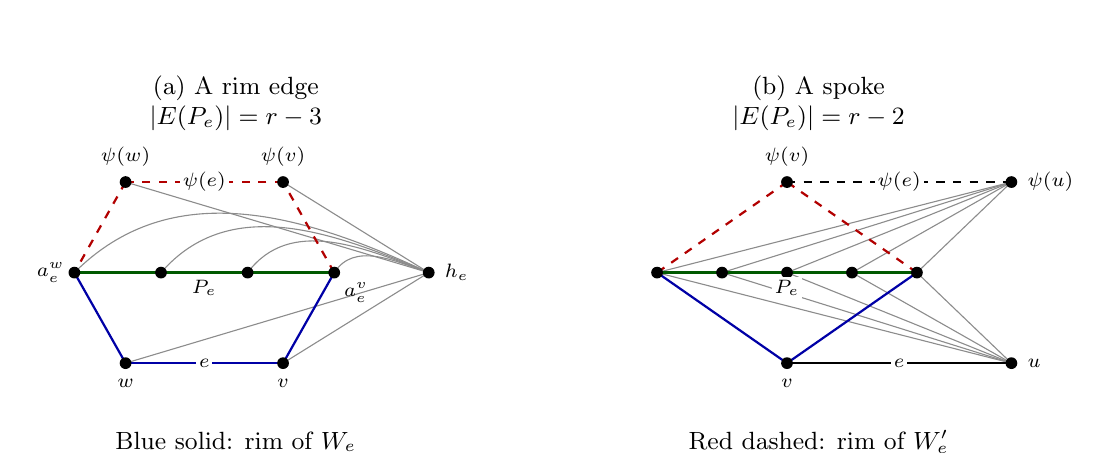
\begin{tikzpicture}[x=1cm,y=1cm,font=\small,>=stealth,
 dot/.style={circle,fill=black,inner sep=1.5pt},
 first/.style={blue!65!black,thick},
 second/.style={red!70!black,thick,dashed},
 shared/.style={green!35!black,very thick},
 spoke/.style={black!45,thin},
 tag/.style={fill=white,inner sep=1pt,font=\scriptsize}]
\begin{scope}[shift={(0,0)},font=\scriptsize]
\coordinate (p0) at (-1.6500,0);
\coordinate (p1) at (-0.5500,0);
\coordinate (p2) at (0.5500,0);
\coordinate (p3) at (1.6500,0);
\coordinate (v) at (1,-1.15); \coordinate (w) at (-1,-1.15);
\coordinate (vp) at (1,1.15); \coordinate (wp) at (-1,1.15);
\coordinate (h) at (2.85,0);
\draw[spoke] (p0) to[out=45,in=155] (h);
\draw[spoke] (p1) to[out=49,in=157] (h);
\draw[spoke] (p2) to[out=53,in=159] (h);
\draw[spoke] (p3) to[out=57,in=161] (h);
\draw[spoke] (v)--(h);
\draw[spoke] (w)--(h);
\draw[spoke] (vp)--(h);
\draw[spoke] (wp)--(h);
\draw[first] (v)--(w);
\draw[first] (w)--(p0);
\draw[first] (p3)--(v);
\draw[second] (vp)--(wp);
\draw[second] (wp)--(p0);
\draw[second] (p3)--(vp);
\node[dot,label=right:$h_e$] at (h) {};
\node[dot,label=below:$ v $] at (v) {};
\node[dot,label=below:$ w $] at (w) {};
\node[dot,label=above:$ \psi(v) $] at (vp) {};
\node[dot,label=above:$ \psi(w) $] at (wp) {};
\path (v)--(w) node[tag,midway] {$e$};\path (vp)--(wp) node[tag,midway] {$\psi(e)$};
\draw[shared] (p0)--(p1);
\draw[shared] (p1)--(p2);
\draw[shared] (p2)--(p3);
\node[dot] at (p0) {};
\node[dot] at (p1) {};
\node[dot] at (p2) {};
\node[dot] at (p3) {};
\node[left] at (p0) {$a_e^w$};\node[below right] at (p3) {$a_e^v$};
\node[tag,below] at (0,-.05) {$P_e$};
\end{scope}
\begin{scope}[shift={(7.4,0)},font=\scriptsize]
\coordinate (p0) at (-1.6500,0);
\coordinate (p1) at (-0.8250,0);
\coordinate (p2) at (0.0000,0);
\coordinate (p3) at (0.8250,0);
\coordinate (p4) at (1.6500,0);
\coordinate (v) at (0,-1.15); \coordinate (vp) at (0,1.15);
\coordinate (h) at (2.85,-1.15); \coordinate (hp) at (2.85,1.15);
\draw[spoke] (p0)--(h);
\draw[spoke] (p0)--(hp);
\draw[spoke] (p1)--(h);
\draw[spoke] (p1)--(hp);
\draw[spoke] (p2)--(h);
\draw[spoke] (p2)--(hp);
\draw[spoke] (p3)--(h);
\draw[spoke] (p3)--(hp);
\draw[spoke] (p4)--(h);
\draw[spoke] (p4)--(hp);
\draw[black,thick] (v)--(h);\draw[black,thick,dashed] (vp)--(hp);
\draw[first] (v)--(p0);
\draw[first] (p4)--(v);
\draw[second] (vp)--(p0);
\draw[second] (p4)--(vp);
\node[dot,label=below:$ v $] at (v) {};
\node[dot,label=above:$ \psi(v) $] at (vp) {};
\node[dot,label=right:$ u $] at (h) {};
\node[dot,label=right:$ \psi(u) $] at (hp) {};
\path (v)--(h) node[tag,midway] {$e$};\path (vp)--(hp) node[tag,midway] {$\psi(e)$};
\draw[shared] (p0)--(p1);
\draw[shared] (p1)--(p2);
\draw[shared] (p2)--(p3);
\draw[shared] (p3)--(p4);
\node[dot] at (p0) {};
\node[dot] at (p1) {};
\node[dot] at (p2) {};
\node[dot] at (p3) {};
\node[dot] at (p4) {};
\node[tag,below] at (0,-.05) {$P_e$};
\end{scope}
\node[align=center] at (.4,2.15) {(a) A rim edge\\$|E(P_e)|=r-3$};
\node[align=center] at (7.8,2.15) {(b) A spoke\\$|E(P_e)|=r-2$};
\node at (.4,-2.15) {Blue solid: rim of $W_e$};
\node at (7.8,-2.15) {Red dashed: rim of $W'_e$};

\end{tikzpicture}
\caption{The wheel pairs in the ordinary transformer, illustrated with $r=6$.
For a rim edge the two wheels share $P_e$, the hub $h_e$, and the
spokes from $P_e$ to $h_e$. For a spoke they share $P_e$ but have
hubs $u$ and $\psi(u)$.}
\label{fig:ordinary:transformer-wheel-pairs}
\end{figure}


Neither $x_j^vy_j^v$ nor $z_j^vy_j^v$ belongs to any of the
wheels $W_e,W'_e$ already defined. Indeed $y_j^v=h_{e_{j-1}^v}$,
and $P_{e_{j-1}^v}$ is disjoint from both $P_{e_j^v}$ and the
spoke path containing $z_j^v$. Here, $j-1\ne j$ modulo $d_v$
because $d_v\ge2$.
We join $x_j^v$ to $z_j^v$ by a path of length $r-2$ with new internal
labels in $N_H(y_j^v)$, using the path construction with this one hub.
Let $Q_j^v,Q_j^{\prime v}$ be the wheels obtained by adjoining
$v,\psi(v)$, respectively, as the remaining rim vertex, with hub
$y_j^v$. All these internal labels are new and avoid every $P_e$.

For each nonisolated $u\in U_1$, put $Z_u:=\bigcup_{e\in E(H_1):\,u\in e}V(P_e)$. The sets $Z_u$ are pairwise
disjoint and $F$-independent. Moreover,
\begin{equation*}
 |Z_u|=(r-1)d_{H_1}(u)\le rq_0,\qquad r\mid|Z_u|,\qquad
 Z_u\subseteq T_{u,\psi(u)}\setminus I_V.
\end{equation*}
We apply Claim~\ref{clm:ordinary:two-factors} successively to
$(u,\psi(u),Z_u)$. In that claim take $X$ to contain all current
rim roots, $X_{\rm ex}\cap V$ and every rim vertex used so far,
and take $\mathcal B$ to be $\mathcal F_{\rm ex}$ together with
all rim edges already used, including the root rim edges.
These sets have size at most $B_*$. The two spokes at each
$z\in Z_u$ avoid $\mathcal F_{\rm ex}$ by the path choices.
The added rim edges do not forbid the spokes $uz,\psi(u)z$
for $z\in Z_u$.
The claim gives $S_u$ and edge-disjoint factors $D_u^1,D_u^2$ on
$S_u\cup Z_u,S_u$, respectively, with every cycle of $D_u^1$
meeting $Z_u$ at most once. Let $B_u^i$ be the wheel family with
rims $D_u^i$ and hub $u$, and let $B_u^{\prime i}$ use hub $\psi(u)$.
The sets $S_u\cup Z_u$ are pairwise disjoint as $u$ varies.

\paragraph{The two decompositions for $r\ge4$.}
For an edge set $A$, let $\chi_A$ be its indicator vector.
For a graph or wheel $W$, write $\chi_W:=\chi_{E(W)}$.
For a wheel family $\mathcal F$, put
$\chi_{\mathcal F}:=\sum_{W\in\mathcal F}\chi_W$. Define
\begin{equation*}
 \Xi_E:=\sum_{e\in E(L_1)}\chi_{W_e},\quad
 \Xi'_E:=\sum_{e\in E(L_1)}\chi_{W'_e},\quad
 \Xi_Q:=\sum_{v,j}\chi_{Q_j^v},\quad
 \Xi'_Q:=\sum_{v,j}\chi_{Q_j^{\prime v}}.
\end{equation*}
Comparison of the root incidences gives
\begin{equation*}
\Xi_E-\Xi'_E-(\Xi_Q-\Xi'_Q)
 =\chi_{L_1}-\chi_{L_2}
   +\sum_{u\in U_1}\sum_{z\in Z_u}
                   (\ind_{uz}-\ind_{\psi(u)z}).
\end{equation*}
For a rim edge $e=vw$, the wheels $W_e,W'_e$ differ on
$e,\psi(e)$, the rim edges
$va_e^v,wa_e^w,\psi(v)a_e^v,\psi(w)a_e^w$, and the spokes
joining $h_e$ to $v,w,\psi(v),\psi(w)$.
For a spoke $e=vu$, they differ on $e,\psi(e)$, the edges
joining $v$ or $\psi(v)$ to an endpoint of $P_e$, and the
spokes joining vertices of $P_e$ to $u$ or $\psi(u)$.
Subtracting $\Xi_Q-\Xi'_Q$ cancels the listed edges joining
path endpoints to vertices of $L_1\cup L_2$, as well as the
listed spokes at $h_e$ for $e\in E(R_1)$.
The remaining terms are $\chi_{L_1}-\chi_{L_2}$ and the
displayed spoke terms indexed by $Z_u$.
Edge-bijectivity gives $\chi_{L_2}$ even when $\psi$ identifies
nonadjacent roots.
The two factors give
\begin{equation*}
\sum_u\bigl(\chi_{B_u^1}+\chi_{B_u^{\prime2}}
             -\chi_{B_u^{\prime1}}-\chi_{B_u^2}\bigr)
 =\sum_u\sum_{z\in Z_u}(\ind_{uz}-\ind_{\psi(u)z}),
\end{equation*}
since the rim edges and the spokes on $S_u$ cancel. Hence the families
\begin{equation*}
\mathcal D:=\{W_e\}_e\cup\{Q_j^{\prime v}\}_{v,j} \cup\bigcup_u(B_u^{\prime1}\cup B_u^2),\qquad \mathcal
D':=\{W'_e\}_e\cup\{Q_j^v\}_{v,j} \cup\bigcup_u(B_u^1\cup B_u^{\prime2})
\end{equation*}
satisfy $\chi_{\mathcal D}-\chi_{\mathcal D'}=\chi_{L_1}-\chi_{L_2}$.

Each family is edge-disjoint. The paths $P_e$ have disjoint vertex
sets, and the hubs $h_e$ chosen for rim edges are distinct.
In $\mathcal D$, each $Q_j^{\prime v}$ uses the root $\psi(v)\in V_2$,
whereas the wheels $W_e$ use roots in $V_1\cup U_1$.
Thus its edges from $\psi(v)$ to its path and hub are absent from
the $W_e$. Its two endpoint spokes are absent by the cyclic shift,
and its other edges meet the internal vertices of the $x_j^v$--$z_j^v$
path, which avoid every $P_e$.
If $h_e$, for $e=vw$, is used by both $Q_{i+1}^{\prime v}$ and
$Q_{\ell+1}^{\prime w}$, their roots are distinct:
$\psi(v)\ne\psi(w)$ because $\psi(e)$ is an edge of the loopless
graph $R_2$. Their path endpoints are also distinct.
The wheels in $B_u^{\prime1}$ use hub $\psi(u)$ on $Z_u$, whereas
$W_{vu}$ uses hub $u$. The spokes on $S_u$ are new, and every
rim edge of $D_u^1$ or $D_u^2$ meets $S_u$.
The factors $D_u^1,D_u^2$ are edge-disjoint, and the sets
$S_u\cup Z_u$ are disjoint for distinct $u$, even if their image
hubs under $\psi$ coincide. This proves edge-disjointness of $\mathcal D$.
In $\mathcal D'$, the wheels $W'_e$ use the root edges $\psi(e)$,
which are distinct by edge-bijectivity, while $Q_j^v$ uses $v\in V_1$.
The same cyclic shift excludes their shared endpoint spokes.
The wheels in $B_u^1$ use hub $u$ on $Z_u$, while $W'_{vu}$ uses
$\psi(u)$, and the sets $S_u\cup Z_u$ remain disjoint.
These facts give edge-disjointness of $\mathcal D'$ without requiring
$\psi$ to be vertex-injective.

The only root-to-root edges of $\mathcal D$ are those of $L_1$,
and those of $\mathcal D'$ are exactly $L_2$. Therefore $T:=\bigcup\mathcal D-L_1=\bigcup\mathcal D'-L_2$ is a
simple graph and the displayed families decompose $T\cup L_1$
and $T\cup L_2$.

\paragraph{The construction for $r=3$.}
For every nonisolated $v\in V_1$, put $I_v:=\{e\in E(R_1):v\in e\}$ and $d_v:=|I_v|=2d_{H_1}(v)\ge2$. We choose a
permutation $\sigma_v$ consisting of one cycle on $I_v$.
In particular $\sigma_v(e)\ne e$. We choose a bijection
$g_v:E_{H_1}(v)\times\{0,1\}\to I_v$, and for $f=vu\in E(H_1)$
write $g_i(f):=g_v(f,i)$.
For $e=vw\in E(R_1)$ choose a new $p_e\in N_R(\{v,w,\psi(v),\psi(w)\})$. For $f=vu\in E(H_1)$ choose new
$a_f,b_f\in N_H(u)\cap N_H(\psi(u))$
with
\begin{equation*}
 \{v,\psi(v),p_{g_0(f)}\}\subseteq N_R(a_f),\qquad
 \{v,\psi(v),p_{g_1(f)},a_f\}\subseteq N_R(b_f).
\end{equation*}
These use at most four rim conditions and two spoke conditions,
so \eqref{eq:ordinary:absorber-row-choice} applies with $k_3=4$.
Put $z_{v,g_0(f)}:=a_f$ and $z_{v,g_1(f)}:=b_f$.

For each $e=vw\in E(R_1)$ we choose a hub $y_e$ adjacent to
\begin{equation*}
 v,w,\psi(v),\psi(w),p_e,
 p_{\sigma_v(e)},z_{v,\sigma_v(e)},
 p_{\sigma_w(e)},z_{w,\sigma_w(e)}.
\end{equation*}
There are at most nine labels, equal to $r+6$ in this case.
The four old labels are $F$-independent by the claim's hypothesis,
and every other label is new and separated from all the others.
Equation~\eqref{eq:ordinary:absorber-hub-choice} supplies such a hub
outside the root hubs and all hubs already chosen.

Write $(x,a,b;u)$ for the triangular wheel with rim $xabx$ and hub $u$.
For $e\in E(R_1)$ and $f\in E(H_1)$, define the wheels
\begin{equation*}
 \begin{aligned}
 E_e&:=(v,p_e,w;y_e),&
 E'_e&:=(\psi(v),p_e,\psi(w);y_e)&& (e=vw\in E(R_1)),\\
 E_f&:=(v,a_f,b_f;u),&
 E'_f&:=(\psi(v),a_f,b_f;\psi(u))&& (f=vu\in E(H_1)).
 \end{aligned}
\end{equation*}
Let $\mathcal E,\mathcal E'$ be the respective families.
For every nonisolated $v\in V_1$ and every $g\in I_v$, let
$Q_{v,g}:=(v,p_g,z_{v,g};y_{\sigma_v^{-1}(g)})$ and
$Q'_{v,g}:=(\psi(v),p_g,z_{v,g};y_{\sigma_v^{-1}(g)})$.
Let $\mathcal Q,\mathcal Q'$ be these families.

For each nonisolated $u\in U_1$ put $Z_u:=\{a_f,b_f:f\in E(H_1),\ u\in f\}$. These sets are disjoint, are $F$-independent, and satisfy
$Z_u\subseteq T_{u,\psi(u)}\setminus I_V$ and
$|Z_u|=2d_{H_1}(u)\le3q_0$, divisible by three.
We apply Claim~\ref{clm:ordinary:two-factors} with $r=3$ and roots $Z_u$,
letting $X$ contain all rim roots, $X_{\rm ex}\cap V$ and previously
used rim vertices, and taking $\mathcal B$ to consist of
$\mathcal F_{\rm ex}$ and all rim edges used so far.
Both prescribed spokes at each $z\in Z_u$ avoid
$\mathcal F_{\rm ex}$ by the choices of $a_f,b_f$. The added
forbidden rim edges do not affect this assertion.
The claim supplies factors $D_u^1,D_u^2$ on $S_u\cup Z_u,S_u$,
with disjoint edges and no cycle of $D_u^1$ meeting $Z_u$ twice.
For $i=1,2$, let $\mathcal B_u^i$ lift $D_u^i$ to hub $u$, and
let $\mathcal B_u^{\prime i}$ lift it to $\psi(u)$.

\paragraph{The two decompositions for $r=3$.}
We verify the signed identity before checking disjointness.
For a wheel family $\mathcal A$, let
$\chi_{\mathcal A}:=\sum_{W\in\mathcal A}\mathbf1_{E(W)}$,
allowing multiplicity in this notation. For an edge set use
its indicator. If $x$ is a free vertex in either $V$ or $U$ occurring below, let $\partial_v(x):=\mathbf1_{vx}-\mathbf1_{\psi(v)x}$.
The two coordinates of $\partial_v(x)$ correspond to rim edges when
$x\in V$ and to spokes when $x\in U$.

\begin{itemize}
    \item For $e\in E(R_1)$, subtraction of its two wheels gives $\chi_{E_e}-\chi_{E'_e}=\mathbf1_e-\mathbf1_{\psi(e)}+\sum_{v\in e} (\partial_v(p_e)+\partial_v(y_e))$.
    
    \item For $f=vu\in E(H_1)$ it gives $\chi_{E_f}-\chi_{E'_f}=\mathbf1_f-\mathbf1_{\psi(f)}+\partial_v(a_f)+\partial_v(b_f)+\sum_{z\in\{a_f,b_f\}}(\mathbf1_{uz}-\mathbf1_{\psi(u)z})$.
    
    \item For the pair $Q_{v,g},Q'_{v,g}$, the difference is $\chi_{Q_{v,g}}-\chi_{Q'_{v,g}} =\partial_v(p_g)+\partial_v(z_{v,g})+\partial_v(y_{\sigma_v^{-1}(g)})$.
\end{itemize}

Since $\sigma_v$ and $g_v$ are bijections, summing these formulas gives
\begin{equation}\label{eq:new:triangle:joint-identity}
 \chi_{\mathcal E}-\chi_{\mathcal E'}-\chi_{\mathcal Q}+\chi_{\mathcal Q'} =\chi_{L_1}-\chi_{L_2}+\sum_u\sum_{z\in Z_u}(\mathbf1_{uz}-\mathbf1_{\psi(u)z}),
\end{equation}
where the use of $\chi_{L_2}$ is justified by the edge
bijection, even when $\psi$ identifies nonadjacent roots.
The two factors on $S_u$ and $S_u\cup Z_u$ give the identity
\begin{equation}
 \chi_{\mathcal B_u^1}+\chi_{\mathcal B_u^{\prime2}}
 -\chi_{\mathcal B_u^{\prime1}}-\chi_{\mathcal B_u^2}
 =\sum_{z\in Z_u}(\mathbf1_{uz}-\mathbf1_{\psi(u)z}).
 \label{eq:new:triangle:cleanup-identity}
\end{equation}

Their rim edges cancel, and each wheel has exactly one spoke at each vertex of its rim, which proves this identity.

Define two families $\mathcal D := \mathcal E\cup\mathcal Q' \cup\bigcup_u(\mathcal B_u^{\prime1}\cup\mathcal B_u^2)$
and
$\mathcal D' :=\mathcal E'\cup\mathcal Q \cup\bigcup_u(\mathcal B_u^1\cup\mathcal B_u^{\prime2})$.

We check edge-disjointness for $\mathcal D$. For $\mathcal D'$,
the four constituent families
$\mathcal E,\mathcal Q',\mathcal B_u^{\prime1},\mathcal B_u^2$
are replaced by
$\mathcal E',\mathcal Q,\mathcal B_u^1,\mathcal B_u^{\prime2}$,
respectively, with the same indices $u,e,g$ and the same map $\psi$.
At $y_e$, the root spokes then have endpoints
$\psi(v),\psi(w),v,w$, the same four distinct vertices as for $\mathcal D$.
The disjoint sets $S_u\cup Z_u$ remain indexed by $u\in U_1$,
also when two such vertices have the same image under $\psi$.
The edges of $\mathcal E$ with both endpoints in the root sets are
precisely the distinct edges of $L_1$. Its rim edges with exactly one
root endpoint have the form $vp_g$ or $vz_{v,g}$, with $v\in V_1$.
The corresponding edges in $\mathcal Q'$ are $\psi(v)p_g$ and
$\psi(v)z_{v,g}$, with $\psi(v)\in V_2$.
Within $\mathcal Q'$, the root neighbors of $p_g$ are the images
of the two endpoints of $g$, which are distinct, and each $z_{v,g}$
is indexed by a single pair $(v,g)$.
This excludes repetitions of all these edges, including
when other roots have the same image under $\psi$.

At the vertex $y_e\in U$, where $e=vw$, the three possible
wheels of $\mathcal D$ are $E_e$,
$Q'_{v,\sigma_v(e)}$, and $Q'_{w,\sigma_w(e)}$.
Their root spokes go respectively to $v,w$ and to
$\psi(v),\psi(w)$, four distinct roots.
Their other spoke endpoints are
$p_e$, $p_{\sigma_v(e)}$, $z_{v,\sigma_v(e)}$, $p_{\sigma_w(e)}$ and $z_{w,\sigma_w(e)}$. These are distinct.
The two permuted edges differ from
$e$. If they were equal to each other, they would form
another edge joining $v,w$, contrary to simplicity of
$R_1$. All $z$-labels are distinct and differ from
all $p$-labels. Thus no spoke at $y_e$ is repeated.
Before the factors on $S_u$ and $S_u\cup Z_u$ are added, the only
edges within the free vertices of $V$ are
$a_fb_f$ and $p_gz_{v,g}$. Within each family the edges
are distinct. Every edge of the second family contains a $p$-label,
whereas no edge of the first family does, so the two families are disjoint.

It remains to check the wheels formed from the two factors. Their rim edges
meet the set $S_u$ supplied by Claim~\ref{clm:ordinary:two-factors},
which avoids all earlier rim vertices. The two factors at
this set are edge-disjoint. Different $u$ have disjoint
sets $S_u\cup Z_u$. A spoke from $Z_u$ occurs in
$\mathcal E$ at hub $u$, and in the factor wheels of
$\mathcal D$ at the different hub $\psi(u)$.
The spokes from $S_u$ occur once at each of these two
hubs. Even if two vertices of $U_1$ have the same image, their
sets $S_u\cup Z_u$ are disjoint. No edge of these factor wheels can
coincide with an edge of $Q_{v,g}$ or $Q'_{v,g}$, since the latter
wheels have new hubs and their rim edges have both endpoints outside
every $S_u$.
This completes the edge-disjointness check.

Equations~\eqref{eq:new:triangle:joint-identity}--
\eqref{eq:new:triangle:cleanup-identity} now imply
$\chi_{\mathcal D}-\chi_{\mathcal D'}=\chi_{L_1}-\chi_{L_2}$. The root edges in $\mathcal D$ are exactly
$L_1$, and
those in $\mathcal D'$ are exactly $L_2$.
Consequently their remaining edge sets are equal. We denote this simple graph by $T$. The displayed families decompose
$L_1\cup T$ and $L_2\cup T$, respectively.
Every edge of $T$ has a new endpoint.


\paragraph{The size of the transformer and avoidance of forbidden sets.}
Put $a:=e(R_1)=e(H_1)\le q_0^2$.
For $r\ge4$, the rim paths, spoke paths, internal paths of the
wheels $Q_j^v$, and new hubs use, respectively, at most
$(r-2)a,(r-1)a,2(r-3)a,a$ vertices. For $r=3$, there are $a$ labels $p_e$, $2a$ labels $a_f,b_f$,
and $a$ hubs $y_e$.
There are at most $q_0$ factor sets $S_u$, each of size $rt_{\rm cl}$.
Both cases therefore use at most
$10r q_0^2+rt_{\rm cl}q_0=K_{\rm tr}$ new vertices.
This also validates every preceding exclusion bound: external
exclusions contribute at most $B_{\rm ex}$, the roots and new
vertices at most $2q_0+K_{\rm tr}$, and all edges on these vertices
at most $4(2q_0+K_{\rm tr})^2$.

Every edge of $T$ is either a newly prescribed edge, a factor rim
edge, or a factor spoke. The choices and
Claim~\ref{clm:ordinary:two-factors} make them all avoid
$\mathcal F_{\rm ex}$. Every such edge has a new endpoint.
The vertex choices guaranteed by \eqref{eq:ordinary:absorber-row-choice}
and the separation conclusion of that claim give
mutual separation of the new rim vertices and their separation from
all rim roots. Only the fixed root edges may meet
$\mathcal F_{\rm ex}$. This proves the transformer claim.
\end{proof}

\paragraph{Assembling the absorber.}
Let $\mathcal G_5$ be the union of the five embedded graphs in
\eqref{eq:ordinary:four-maps}. We apply
Claim~\ref{clm:ordinary:rooted-transformer} to the four maps in that
display, in order, obtaining $T_1,\ldots,T_4$. At step $j$, define
\begin{equation*}
 X_{\rm ex} := I_0\cup V(\mathcal G_5)\cup\bigcup_{h<j}V(T_h),\qquad
 \mathcal F_{\rm ex} := F_0\cup E(\mathcal G_5)\cup\bigcup_{h<j}E(T_h).
\end{equation*}
The internal vertex and edge sets here lie on at most $m_0+M$
vertices, so their total size, together with $|I_0|+|F_0|\le f$,
is at most $B_{\rm ex}$. Each source has order at most $q_0$,
is $r$-wheel-divisible, and satisfies
\eqref{eq:ordinary:edgewise-root-separation} with its image.
Thus every hypothesis of the claim holds at each application.
New transformer vertices avoid the five graphs and the earlier
transformers, and their edges avoid all earlier edges. In particular,
the component edge sets in $A_L:=(L_{\rm att}-L)\cup T_1\cup L'_{\rm exp}\cup T_2\cup\Gamma \cup T_3\cup J'_{\rm exp}\cup T_4\cup J_{\rm att}$
are disjoint.
A wheel decomposition of $A_L$ is obtained from
\begin{equation*}
L_{\rm att}-L,\quad T_1\cup L'_{\rm exp},\quad
 T_2\cup\Gamma,\quad T_3\cup J'_{\rm exp},\quad T_4\cup J_{\rm att}.
\end{equation*}
The first graph is the union of the attachment wheels. Each of the
other four has a wheel decomposition by
Claim~\ref{clm:ordinary:rooted-transformer}.
A wheel decomposition of $A_L\cup L$ is obtained from
\begin{equation*}
L_{\rm att}\cup T_1,\quad L'_{\rm exp}\cup T_2,\quad
 \Gamma\cup T_3,\quad J'_{\rm exp}\cup T_4,\quad J_{\rm att}.
\end{equation*}
The first four graphs have wheel decompositions by the same claim,
and $J_{\rm att}$ is a wheel union. Each display partitions the indicated edge set.

Only $L_{\rm att}$ among the five graphs meets the original roots,
and every edge of $L_{\rm att}-L$ has a new endpoint.
Every transformer edge has an endpoint outside the five graphs.
Consequently $E(A_L[V(L)])=\varnothing$, and $A_L$ is edge-disjoint
from $L$. All newly constructed edges avoid $F_0$, and all new
vertices avoid $I_V\cup I_U\cup I_0$.
There are at most $5q_0$ vertices in the five graphs and at most
$4K_{\rm tr}$ new transformer vertices, giving the bound $M$ in
\eqref{eq:ordinary:absorber-size}.
This proves the theorem.
\end{proof}

\section{Covering the spokes at a prescribed hub}
\label{sec:new:hub-factors}

Let $\mathcal Q$ be a fixed typed extended graph with auxiliary arc graphs
$R_{\mathcal Q}^0,R_{\mathcal Q}^K$ on $V$ and bipartite graphs
$H_{\mathcal Q}^{0},H_{\mathcal Q}^{K}$ between $V$ and $W$.
For $w\in W$, let $Y:=N_{H_{\mathcal Q}^{K}}(w)$ and $O:=N_{H_{\mathcal Q}^{0}}(w)$. A cycle $C$ with
$(C,w)\in\mathcal W_c^K(\mathcal Q)$ has one marked
arc with head in $Y$ and all its other vertices in $O$.
To cover the edges of $H_{\mathcal Q}^{0}\cup H_{\mathcal Q}^{K}$
incident with $w$, we need the ratio $|O|=(c-1)|Y|$, but no
divisibility condition on the arc graphs. The wheel weights induce
cycle weights whose sum at each rim vertex is close to one.
Together with the absorber counts obtained below, these weights
allow us to apply Lemma~\ref{lem:simp:profile-factor} with class
sizes $(1,c-1)$ and obtain a cycle factor on $Y\cup O$.

Let\phantomsection\label{gls:one-hub-marked-cycle-and-common-path-families} $c\ge8$ and $b\ge0$ be integers, and let $\pi$ be a permutation of $V$.
For $w\in W$ let
\begin{equation}
 \mathcal C_w:=\{C:(C,w)\in\mathcal W_c^K(\mathcal Q;b,\pi)\}.
 \label{eq:marked:one-hub-cycles}
\end{equation}
For\phantomsection\label{gls:one-hub-marked-cycle-and-common-path-families:paths} distinct $v,v'\in V$ and $j\in\{0,K\}$, let
$\mathcal F_j(v,v';w)$ be the family of ordered tuples
$\mathbf z=(z_1,\ldots,z_{c-1})$ of distinct vertices in
$V\setminus\{v,v'\}$ satisfying the following conditions.
The vertices $z_1,\ldots,z_{c-1}$ are mutually $(b,\pi)$-separated,
and each is $(b,\pi)$-separated from both $v$ and $v'$.
The cycles $C_1:=C_j(v,\mathbf z)$ and $C_2:=C_j(v',\mathbf z)$
have their prescribed typed arcs in
$R^0_{\mathcal Q}\dot\cup R^K_{\mathcal Q}$, and
\begin{equation}
\begin{gathered}
 z_iw\in E(H^{t_{C_1}(z_i)}_{\mathcal Q})\quad(1\le i<c),\\
 |\operatorname{phys}(E(C_\ell))|=c,\quad |\operatorname{phys}(e)|=2
       \quad(\ell=1,2;\ e\in E(C_\ell)),\\
 \operatorname{phys}(e)=\operatorname{phys}(f)\ \Longrightarrow\
 (\operatorname{tail}(e),\operatorname{type}(e))
 =(\operatorname{tail}(f),\operatorname{type}(f))
       \quad(e\in E(C_1),\ f\in E(C_2)).
\end{gathered}
 \label{eq:marked:one-hub-paths}
\end{equation}
Here, $C_j(v,\mathbf z)$ has its marked arc into $v$ if $j=K$
and at $z_2\to z_3$ if $j=0$, and $\operatorname{phys}$ is the physical image
map \eqref{eq:physical:image-map}. Neither root spoke is required,
and no separation between $v$ and $v'$ is imposed.

Recall that a member of $\mathcal A_{\mathcal C_w}(X)$ in
\eqref{eq:paired-absorbers:two-classes} specifies paired cycle factors
from $\mathcal C_w$ on a free vertex set and on its union with $X$.
The free set is disjoint from $X$ and has $c$ vertices in $Y$ and
$c(c-1)$ in $O$. The count retains all prescribed label orderings
and cycle identifiers.

\begin{lemma}
\label{lem:local:marked-hub-absorbers}
Let $c\ge8$ be an integer and let $\beta>0$. There exists $a>0$ such that for every integer $b\ge1$ there is $n_0\in\mathbb N$ for which the following holds for $n\ge n_0$.

Let $V,W$ be disjoint sets and let $\pi$ be a permutation of $V$.
Let $\mathcal Q=(R^0,R^K,H^0,H^K)$ be a physically injective typed extended graph on $(V,W,\pi)$, with $|V|=n$, and let $w\in W$.
Let $Y:=N_{H^{K}_{\mathcal Q}}(w)$ and
$O:=N_{H^{0}_{\mathcal Q}}(w)$, and assume $|Y|,|O|\ge\beta n$.
Let $\mathcal C_w$ and $\mathcal F_j(v,v';w)$ be defined by~\eqref{eq:marked:one-hub-cycles} and~\eqref{eq:marked:one-hub-paths}, respectively.

Suppose $|\mathcal C_w|\ge\beta n^c$, $|\mathcal F_K(v,v';w)|\ge\beta n^{c-1}$ for all $v\ne v'\in Y$, and
$|\mathcal F_0(v,v';w)|\ge\beta n^{c-1}$ for all $v\ne v'\in O$.
Then $|\mathcal A_{\mathcal C_w}(X)|\ge an^{c^2}$ for every
$X\subseteq Y\cup O$ with $|X\cap Y|=1$ and $|X\cap O|=c-1$,
where $\mathcal A_{\mathcal C_w}(X)$ is the restricted paired-absorber
family in \eqref{eq:paired-absorbers:two-classes}, with classes $(Y,O)$.
\end{lemma}
\begin{proof}
Fix $X\in\mathcal R_{c-1}(Y,O)$ and order it as
$x_0,\ldots,x_{c-1}$, with $x_0\in Y$ and $x_i\in O$ for $i>0$.
The set $\{z\in V:\operatorname{dist}_\pi(z,x)\le b
\text{ for some }x\in X\}$ has size at most $c(2b+1)$.
At most $O_{c,b}(n^{c-1})$ cycles of $\mathcal C_w$ meet this set,
so at least $\beta n^c/2$ choices of a base cycle $C_*$ avoid it
for large $n$. For each $C_*$, put $y_0:=y_{C_*}$ and order its
remaining vertices as $y_1,\ldots,y_{c-1}$ in a fixed way.

For $i=0$ we choose $\mathbf z_i\in\mathcal F_K(x_i,y_i;w)$,
and for $i>0$ we choose $\mathbf z_i\in\mathcal F_0(x_i,y_i;w)$.
Its vertices avoid $X$, $V(C_*)$ and all previously chosen
$\mathbf z_j$. Excluding these bounded sets removes at most
$O_c(n^{c-2})$ tuples, since a specified forbidden vertex fixes
one of the $c-1$ positions. Each choice therefore has at least
$\beta n^{c-1}/2$ possibilities. The two cycles obtained by adjoining
$x_i$ and $y_i$ both belong to $\mathcal C_w$: the tuple supplies
their typed arcs and free spokes, and the two root spokes have the
required type because $x_i,y_i$ lie in the same class $Y$ or $O$.
These cycles and $C_*$ form the paired absorber in
\eqref{eq:cycle:paired-absorbers}, with all free vertices distinct.
Its ordered labels and cycle identifiers retain every choice.
Thus there are at least $(\beta/2)^{c+1}n^{c^2}$ such labeled
absorbers. We may take $a=(\beta/2)^{c+1}$.

\end{proof}


\Needspace{8\baselineskip}
\begin{lemma}
\label{lem:completion:marked-hub-factor}
Let $c\ge8$ be an integer, and let $\beta>0$ and $B_{\omega}>1$. There exists $\eta_*>0$ such that for every fixed separation
distance $b\in\mathbb Z_{\ge1}$ there is $n_0\in\mathbb N$ for which the following holds
for $n\ge n_0$. Let $V,W$ be disjoint sets with $|V|=n$, let
$\pi$ be a permutation of $V$, and let
$\mathcal Q=(R^0,R^K,H^0,H^K)$ be a physically injective typed
extended graph on $(V,W,\pi)$.

Let $w\in W$, $Y:=N_{H^K}(w)$ and $O:=N_{H^0}(w)$. Let $\mathcal C_w$
and $\mathcal F_j(v,v';w)$ be the families in~\eqref{eq:marked:one-hub-cycles} and~\eqref{eq:marked:one-hub-paths}.
Assume $|Y|,|O|\ge\beta n$, $|\mathcal C_w|\ge\beta n^c$, and
\begin{equation*}
 |\mathcal F_K(v,v';w)|\ge\beta n^{c-1}\quad(v\ne v'\in Y),\qquad
 |\mathcal F_0(v,v';w)|\ge\beta n^{c-1}\quad(v\ne v'\in O),
\end{equation*}
and
\begin{equation}
 |O|=(c-1)|Y|,\qquad O\cap\pi(Y)=\varnothing.
\end{equation}

Let $\phi:\mathcal C_w\to\mathbb R_{\ge0}$ satisfy $B_{\omega}^{-1}n^{1-c}\le\phi(C)\le B_{\omega}n^{1-c}$ for all $C \in \mathcal C_w$
and $\sum_{C\ni v}\phi(C)=1\pm \eta_*$ for all $v \in Y \cup O$.
Then there is a family $\mathcal P\subseteq\mathcal C_w$ such that
\begin{itemize}
    \item $Y\dot\cup O=\mathop{\dot\bigcup}_{C\in\mathcal P}V(C)$;
    
    \item The wheels $\{W(C,w):C\in\mathcal P\}$ cover every spoke at $w$ once, and their physical rim edges are distinct;

    \item The graph $G_w:=(V,\bigcup_{C\in\mathcal P}E_{\rm phys}(C))$ satisfies $\Delta(G_w)\le2$.
\end{itemize}
\end{lemma}
\begin{proof}
Let $a>0$ be supplied by Lemma~\ref{lem:local:marked-hub-absorbers}.
Physical injectivity gives at most one arc of each type with any
specified tail and head. Thus each $c$-vertex set supports at most
$c!$ directed cycles with exactly one marked arc.
The paired absorbers in \eqref{eq:paired-absorbers:two-classes},
with $r=c-1$ and classes $Y,O$, determine a fixed finite family of
absorber templates with class sizes $(1,c-1)$.
We choose $\eta_*$ to be a tolerance supplied by
Lemma~\ref{lem:simp:profile-factor} with these templates,
multiplicity bound $J=c!$, coefficient bound
$B_{\omega}\beta^{1-c}$, and absorber coefficient $a$.

Put $k:=|Y|$. Since $\beta n\le k\le n$, we have
\begin{equation*}
 B_{\omega}^{-1}\beta^{c-1}k^{1-c}\le\phi(C)\le B_{\omega}k^{1-c},\qquad
 |\mathcal A_{\mathcal C_w}(X)|\ge an^{c^2}\ge ak^{c^2}.
\end{equation*}
Moreover $|O|=(c-1)k$. For sufficiently large $n$, we may therefore
apply Lemma~\ref{lem:simp:profile-factor} at scale $k$, with classes
$Y,O$, multiplicities $(1,c-1)$ and weighting $\phi$.
It gives a factor $\mathcal P\subseteq\mathcal C_w$.
For each $C\in\mathcal P$, the wheel $W(C,w)$ consists of $C$
and the spokes $vw$ for $v\in V(C)$.

The cycles in $\mathcal P$ are vertex-disjoint, so their arcs are
pairwise distinct. Physical injectivity of $\mathcal Q$ implies that the
corresponding physical rim edges are also pairwise distinct. Each vertex
of $O$ is incident with one incoming unmarked arc and one outgoing arc,
and each vertex of $Y$ with one outgoing unmarked arc and one incoming
marked arc. The latter arc has physical head in $\pi(Y)$. Consequently,
$d_{G_w}(z)=2\mathbf1_{z\in O}+\mathbf1_{z\in Y} +\mathbf1_{z\in\pi(Y)}\le2$ for all $z\in V$, since
$O\cap Y=O\cap\pi(Y)=\varnothing$ and $\pi$ is a bijection.
\end{proof}

\section{Pairing the rim arcs at a prescribed vertex}
The degree identities of \eqref{eq:typed:imbalance} do not alone
ensure that incoming and outgoing arcs can be assigned to spokes
of a marked wheel. For example, let $c\ge3$ be an integer, let $R^K$ be a directed triangle,
let $R^0$ be a disjoint directed cycle of length $3(c-1)$, and let $U:=\{u\}$.
The spokes from $u$ to $V(R^K)$ have type $K$, and those to $V(R^0)$ have type $0$.
All four degree differences vanish. At a triangle vertex both rim
arcs have type $K$, so no marked $c$-wheel can contain them both.
Lemma~\ref{lem:four:typed-pairing} uses a bound on the total number of marked
arc indices, as well as degree and cut bounds on five bipartite graphs.

\begin{definition}[Marked endpoint assignment graphs]\label{gls:marked-endpoint-assignment-graphs}
\label{def:endpoints:assignment-graphs}
Let\phantomsection\label{gls:marked-endpoint-assignment-graphs:potential-rims} $V,U$ be disjoint finite sets, let $P$ be a simple graph on $V$,
let $\pi$ be a permutation of $V$, and let $d\ge0$.
We define the potential arc sets by
\begin{equation}
\begin{aligned}
 E(\overline R^0)&:=\{v\to w:vw\in E(P),\ \operatorname{dist}_\pi(v,w)>3d\},\\
 E(\overline R^K)&:=\{v\to w:v\pi(w)\in E(P),\ \operatorname{dist}_\pi(v,w)>3d\}.
\end{aligned}
\label{eq:endpoints:potential-rims}
\end{equation}
An arc $v\to w$ of type $K$ has auxiliary head $w$ and physical
edge $\{v,\pi(w)\}$. Let
$\mathcal Q=(R^0,R^K,H^0,H^K)$ have $R^j\subseteq\overline R^j$
and spoke graphs $H^j$ on $(V,U)$.
Let $A\subseteq V$ with $\pi(A)=A$, $B\subseteq U$, and $x\in V$.
For $j\in\{0,K\}$ let
\begin{equation*}
\begin{aligned}
 \overline A_j(x)&:=\{v\to x\in E(\overline R^j):v\in A\},&
 A_j(x)&:=\overline A_j(x)\cap E(R^j),\\
 \overline X_j(x)&:=\{x\to v\in E(\overline R^j):v\in A\},&
 X_j(x)&:=\overline X_j(x)\cap E(R^j),\\
 Y_j(x)&:=\{u\in B:xu\in E(H^j)\}.&&
\end{aligned}
\end{equation*}
The sets $P_{x,i}$ consist of arc occurrences, and
$\overline P_{x,i}$ are the corresponding sets of potential occurrences.
Occurrences with the same endpoint label remain distinct.
The five pairs of actual parts $(P_{x,i},Q_{x,i})$ are given below.
For target spoke densities $s,t\in[0,1]$, the last two columns give
the density $r_i$ at $x$ and the density $z_i$ at the other endpoint.
\begin{equation}
\begin{array}{c|c|c|c|c|c}
 i&P_{x,i}&Q_{x,i}&\overline P_{x,i}&r_i&z_i\\\hline
 1&A_K(x)&Y_K(x)&\overline A_K(x)&t&s\\
 2&A_0(x)&Y_0(x)&\overline A_0(x)&s&s\\
 3&X_K(x)&Y_0(x)&\overline X_K(x)&s&t\\
 4&X_0(x)&Y_0(x)&\overline X_0(x)&s&s\\
 5&X_0(x)&Y_K(x)&\overline X_0(x)&t&s
\end{array}
\label{eq:endpoints:index-table}
\end{equation}
Define $\ell_{x,i}:\overline P_{x,i}\to A$ by
$\ell_{x,i}(v\to x):=v$ for $i=1,2$ and
$\ell_{x,i}(x\to v):=v$ for $i=3,4,5$.
The same notation denotes its restriction to $P_{x,i}$. Let $\tau_3:=K$ and $\tau_i:=0$ for $i\ne3$.
The\phantomsection\label{gls:marked-endpoint-assignment-graphs:potential} potential bipartite graph $\overline D_{x,i}$ has parts
$(\overline P_{x,i},B)$, with
\begin{equation*}
a'u\in E(\overline D_{x,i})\quad\Longleftrightarrow\quad
 \ell_{x,i}(a')u\in E(H^{\tau_i})
 \quad(a'\in\overline P_{x,i},\ u\in B).
\end{equation*}
The \emph{marked endpoint assignment graph} is
$D_{x,i}:=\overline D_{x,i}[P_{x,i},Q_{x,i}]$.
For $i=1,2$, an assignment of an arc $v\to x$ to a hub $u$ requires
$vu\in E(H^0)$. For $i=3$, an assignment of an arc $x\to v$
requires $vu\in E(H^K)$, whereas for $i=4,5$ it requires $vu\in E(H^0)$.
In each case the type of $xu$ is specified by $Q_{x,i}$.
We\phantomsection\label{gls:marked-endpoint-assignment-graphs:neighborhoods} define the enlarged neighborhoods by
\begin{equation}
\mathcal N_{x,i}(a'):=N_{\overline D_{x,i}}(a')\cap Q_{x,i} \quad (a'\in\overline P_{x,i}),\qquad \mathcal
M_{x,i}(u):=N_{\overline D_{x,i}}(u)\cap P_{x,i} \quad (u\in B).
\label{eq:endpoints:enlarged-neighbourhoods}
\end{equation}
On the actual parts these are the neighborhoods in $D_{x,i}$.
The first formula also includes absent arc indices, and the second
does not require $xu$ to be a spoke of either type.
For $a'\in\overline P_{x,i}$ let
\begin{equation*}
\mathcal E_{x,i}(a'):=\{a''\in\overline P_{x,i}\setminus\{a'\}:
       \operatorname{dist}_\pi(\ell_{x,i}(a'),\ell_{x,i}(a''))\le3d\}.
\end{equation*}
\end{definition}

Figure~\ref{fig:endpoints:five-assignment-graphs} shows the five pairs
of parts and how the two assignments at a hub specify its paired rim arcs.
\begin{figure}[htbp]
\centering
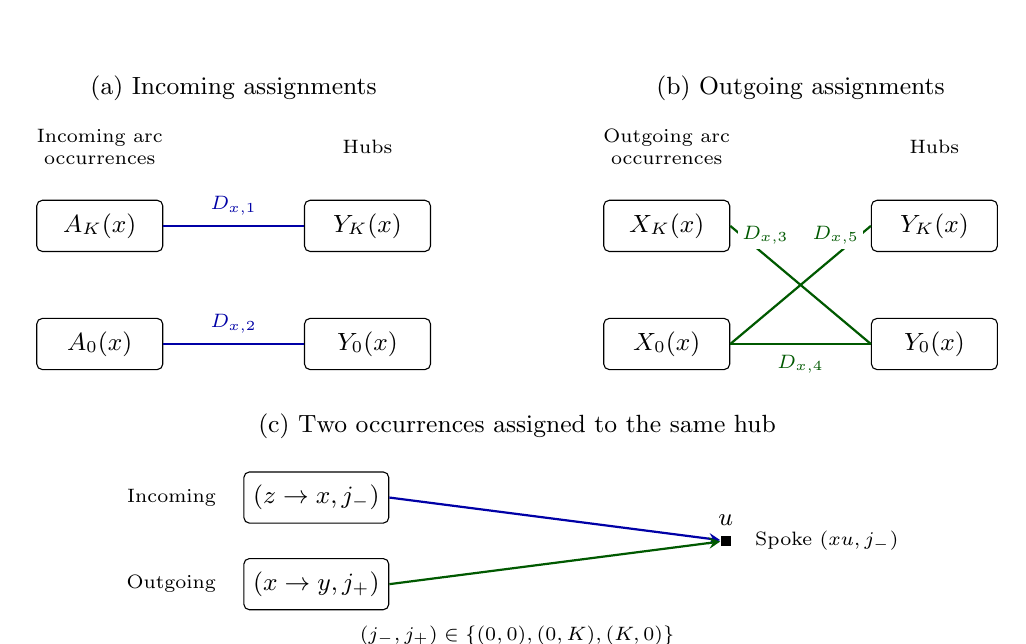
\begin{tikzpicture}[x=1cm,y=1cm,font=\small,>=stealth,
 part/.style={draw,rounded corners=2pt,fill=white,minimum width=1.6cm,
              minimum height=.65cm},
 incoming/.style={blue!65!black,thick},
 outgoing/.style={green!35!black,thick},
 tag/.style={fill=white,inner sep=1.5pt,font=\scriptsize},
 hub/.style={rectangle,fill=black,inner sep=1.8pt}]
\node at (2.15,3.25) {(a) Incoming assignments};
\node at (9.35,3.25) {(b) Outgoing assignments};
\node[font=\scriptsize,align=center] at (.45,2.5) {Incoming arc\\occurrences};
\node[font=\scriptsize] at (3.85,2.5) {Hubs};
\node[font=\scriptsize,align=center] at (7.65,2.5) {Outgoing arc\\occurrences};
\node[font=\scriptsize] at (11.05,2.5) {Hubs};
\node[part] (AK) at (.45,1.5) {$A_K(x)$};
\node[part] (A0) at (.45,0) {$A_0(x)$};
\node[part] (YKleft) at (3.85,1.5) {$Y_K(x)$};
\node[part] (Y0left) at (3.85,0) {$Y_0(x)$};
\draw[incoming] (AK.east)--node[tag,above=2pt] {$D_{x,1}$} (YKleft.west);
\draw[incoming] (A0.east)--node[tag,above=2pt] {$D_{x,2}$} (Y0left.west);
\node[part] (XK) at (7.65,1.5) {$X_K(x)$};
\node[part] (X0) at (7.65,0) {$X_0(x)$};
\node[part] (YKright) at (11.05,1.5) {$Y_K(x)$};
\node[part] (Y0right) at (11.05,0) {$Y_0(x)$};
\draw[outgoing] (XK.east)--node[tag,pos=.25,above=2pt] {$D_{x,3}$} (Y0right.west);
\draw[outgoing] (X0.east)--node[tag,below=2pt] {$D_{x,4}$} (Y0right.west);
\draw[outgoing] (X0.east)--node[tag,pos=.75,above=2pt] {$D_{x,5}$} (YKright.west);

\node at (5.75,-1.05) {(c) Two occurrences assigned to the same hub};
\node[part] (in) at (3.2,-1.95) {$(z\to x,j_-)$};
\node[part] (out) at (3.2,-3.05) {$(x\to y,j_+)$};
\node[font=\scriptsize,anchor=east] at (2.05,-1.95) {Incoming};
\node[font=\scriptsize,anchor=east] at (2.05,-3.05) {Outgoing};
\node[hub,label=above:$u$] (u) at (8.4,-2.5) {};
\draw[incoming,->] (in.east)--(u);
\draw[outgoing,->] (out.east)--(u);
\node[font=\scriptsize,anchor=west] at (8.65,-2.5) {Spoke $(xu,j_-)$};
\node[font=\scriptsize] at (5.75,-3.7)
 {$ (j_-,j_+)\in\{(0,0),(0,K),(K,0)\}$};
\end{tikzpicture}
\caption{Part pairs of the five endpoint assignment graphs.
An incoming and an outgoing arc occurrence assigned to the same hub
determine the two rim arcs paired with its spoke at $x$.}
\label{fig:endpoints:five-assignment-graphs}
\end{figure}

The map $\ell_{x,i}$ is injective, and a $\pi$-distance ball of
radius $3d$ has at most $6d+1$ vertices. Hence
\begin{equation}
 |\mathcal E_{x,i}(a')|\le6d+1
 \quad(x\in V,\ i\in[5],\ a'\in\overline P_{x,i}).
 \label{eq:endpoints:exceptional-bound}
\end{equation}

\Needspace{7\baselineskip}
\begin{lemma}
\label{lem:pairing:degree-cut-hall}
Let $X,Y$ be disjoint finite sets with $|X|=|Y|$, let $s>0$ and
$0<\epsilon<\lambda$, and let $B$ be a bipartite graph on $(X,Y)$.
Suppose every vertex has degree at least $\lambda s$, and
$e_B(P,Q)>0$ whenever $P\subseteq X$, $Q\subseteq Y$ and
$|P|,|Q|\ge\epsilon s$. Then $B\text{ has a perfect matching}$. \end{lemma}
\begin{proof}
Write $\Gamma_B(S):=\bigcup_{x\in S}N_B(x)$.
Suppose Hall's condition fails at $S\subseteq X$.
Then $S\ne\varnothing$ and $T:=Y\setminus \Gamma_B(S)\ne\varnothing$.
If $|S|<\lambda s$, a vertex of $S$ has at least $\lambda s$
neighbors, contradicting $|\Gamma_B(S)|<|S|$.
If $|T|<\lambda s$, every vertex of $T$ has all its neighbors in
$X\setminus S$, whose size is less than $|T|$, again a contradiction.
Otherwise $|S|,|T|\ge\lambda s>\epsilon s$, contrary to
$e_B(S,T)=0$. Hall's theorem (Theorem~\ref{thm:prelim:hall})
therefore gives a perfect matching.
\end{proof}

\Needspace{7\baselineskip}
\begin{lemma}
\label{lem:four:typed-pairing}
Let $b,M\ge1$ be integers, let $\kappa,\lambda>0$, and let
$0<\epsilon<\min\{\kappa,\lambda\}/8$.
There is $s_0\in\mathbb N$ such that the following holds for
integers $s\ge s_0$.
Let $A=A_K\dot\cup A_0$, $X=X_K\dot\cup X_0$ and
$Y=Y_K\dot\cup Y_0$ be finite index sets of size $s$, with
$|A_K|=|Y_K|=k$, $|X_K|=l$ and $k+l\le(1-\kappa)s$. The three index sets are taken as disjoint copies.
Let $\pi$ be a permutation of a finite set $V$, and let
$\ell_A:A\to V$, $\ell_X:X\to V$ satisfy
$|\ell_A^{-1}(v)|,|\ell_X^{-1}(v)|\le M$ for $v\in V$.
Let $B_1,\ldots,B_5$ be bipartite graphs on the ordered pairs
$(A_K,Y_K)$, $(A_0,Y_0)$, $(X_K,Y_0)$, $(X_0,Y_0)$ and $(X_0,Y_K)$, respectively. For each graph $B_i$
on $(P_i,Q_i)$ suppose that
\begin{equation*}
 d_{B_i}(z)\ge2\lambda s\quad(z\in P_i\cup Q_i),\qquad
 e_{B_i}(P,Q)\ge\lambda|P||Q|
 \quad(P\subseteq P_i,\ Q\subseteq Q_i,\ |P|,|Q|\ge\epsilon s).
\end{equation*}
Then there exist bijections $f:A\to Y$ and $g:X\to Y$ such that
\begin{equation*}
\begin{gathered}
 (a,f(a))\in E(B_1)\cup E(B_2)\quad(a\in A),\qquad
 (a,g(a))\in E(B_3)\cup E(B_4)\cup E(B_5)\quad(a\in X),\\
 f(A_K)=Y_K,\qquad g(X_K)\subseteq Y_0,\qquad \operatorname{dist}_\pi\bigl(\ell_A(f^{-1}(y)), \ell_X(g^{-1}(y))\bigr)>b\quad(y\in Y).
\end{gathered}
\end{equation*}
\end{lemma}
\begin{proof}
We choose $s_0$ so that, for $C:=M(2b+1)$ and every $s\ge s_0$, $C\le\lambda s$ and $C<\lambda\epsilon s$. The
graphs $B_1,B_2$ have balanced parts. By
Lemma~\ref{lem:pairing:degree-cut-hall}, each has a perfect matching.
Their union defines $f$.
For $i=3,4,5$, let
\begin{equation*}
 E(\widetilde B_i):=\{ay\in E(B_i):
 \operatorname{dist}_\pi(\ell_X(a),\ell_A(f^{-1}(y)))>b\}.
\end{equation*}
At each $y$ at most $C$ edges are
removed, since a distance ball
contains at most $2b+1$ labels and each label has at most $M$
preimages under $\ell_X$. At each $a\in X$ at most $C$ edges are
removed as well: at most $C$ indices of $A$ have a label in that
ball, and $f$ sends them to distinct vertices of $Y$.
Each $\widetilde B_i$ has minimum degree at least $\lambda s$.
For $P\subseteq P_i$ and $Q\subseteq Q_i$ with
$|P|,|Q|\ge\epsilon s$, we have
$e_{\widetilde B_i}(P,Q)\ge\lambda|P||Q|-C\min\{|P|,|Q|\}>0$,
since $\lambda\epsilon s>C$.

Let $B^+:=\widetilde B_3\cup\widetilde B_4\cup\widetilde B_5$
on $(X,Y)$, and write
$\Gamma_{B^+}(S):=\bigcup_{x\in S}N_{B^+}(x)$.
We verify Hall's condition for nonempty $S\subseteq X$.
Write $S_0:=S\cap X_0$ and $S_K:=S\cap X_K$.
If $|S_0|,|S_K|<\epsilon s$, then
$|S|<2\epsilon s<\lambda s\le|\Gamma_{B^+}(S)|$.

Suppose $|S_0|\ge\epsilon s$. In each of $Y_0,Y_K$ fewer than
$\epsilon s$ vertices can avoid $\Gamma_{B^+}(S)$, by the cut property
in $\widetilde B_4$ and $\widetilde B_5$.
Hence $|\Gamma_{B^+}(S)|>s-2\epsilon s$.
This suffices when $|S|\le s-2\epsilon s$.
Otherwise a vertex outside $\Gamma_{B^+}(S)$ would have all its at least
$\lambda s$ neighbors in $X\setminus S$, a set of size less than
$2\epsilon s$, which is impossible.

Finally, if $|S_0|<\epsilon s\le|S_K|$, the cut property in $\widetilde B_3$
and the inequality $|Y_0|-|X_K|\ge\kappa s$ give
$|\Gamma_{B^+}(S)|>|Y_0|-\epsilon s \ge |X_K|+(\kappa-\epsilon)s>|S_K|+|S_0|$. Hall's theorem (Theorem~\ref{thm:prelim:hall})
supplies a perfect matching of $B^+$,
which defines $g$. Every edge $ay$ of $B^+$ satisfies
$\operatorname{dist}_\pi(\ell_X(a),\ell_A(f^{-1}(y)))>b$,
so this holds with $a=g^{-1}(y)$ for every $y\in Y$.
The parts of $B_1,B_2,\widetilde B_3$ give $f(A_K)=Y_K$ and
$g(X_K)\subseteq Y_0$. 
\end{proof}



\section{Endpoint assignment graphs after random restriction}
We first derive cut estimates from degree and common-neighbor bounds.
We then show that these estimates survive random restriction and
subsequent small changes of both parts. The final lemma verifies
the deterministic hypotheses for the five marked endpoint graphs.

\begin{lemma}
\label{lem:new:cuts-from-codegrees}
Let $m,n\in\mathbb Z_{\ge0}$, $p\in[0,1]$ and $\eta,b\ge0$.
Let $D$ be a bipartite graph on $(A,B)$, where $|A|=m$, $|B|=n$,
and $d_D(x)=(p\pm\eta)n$ for $x\in A$.
Suppose a graph $J$ on $A$, of maximum degree at most $b$, contains
every distinct pair $x,x'$ with
$|N_D(x)\cap N_D(x')|>(p^2+\eta)n$.
Then, for all nonempty $P\subseteq A$ and $Q\subseteq B$,
\begin{equation*}
\bigl|e_D(P,Q)-p|P||Q|\bigr|
 \le |P||Q|\left(\frac{3\eta n}{|Q|}
                  +\frac{(b+1)n}{|P||Q|}\right)^{1/2}.
\end{equation*}
\end{lemma}

The proof is given in Appendix~\ref{app:proof:lem-new-cuts-from-codegrees}.

\Needspace{7\baselineskip}
\begin{theorem}[Degree and cut bounds after random restriction]
\label{thm:new:fresh-candidacy}
Let $0<p_*,a\le1$ and $\epsilon>0$.
There are $\eta_0,\zeta>0$ such that, for every integer $b\ge0$
and every $\rho\in(0,1)$, there is $N_0\in\mathbb N$ with the following property.
Let $D$ be a bipartite graph on $(A,B)$, with
$aN\le m=|A|,n=|B|\le N$, $N\ge N_0$, and $p\in[p_*,1]$.
Suppose
\begin{equation*}
 d_D(x)=(p\pm\eta_0)n\quad(x\in A),\qquad
 d_D(y)=(p\pm\eta_0)m\quad(y\in B).
\end{equation*}
Let $J$ be the graph on $A$ in which distinct $x,x'$ are adjacent
precisely when $|N_D(x)\cap N_D(x')|>(p^2+\eta_0)n$. Assume $\Delta(J)\le b$. Let $m':=\lfloor\rho m\rfloor$, $n':=\lfloor\rho n\rfloor$ and
$s_R:=\min\{m',n'\}$. Let $A'\subseteq A$ and $B'\subseteq B$ be random subsets obtained
by including each vertex of $A\cup B$ independently with probability $\rho$.
With probability at least $1-N^{-10}$, the following holds
simultaneously for every $A''\subseteq A$, $B''\subseteq B$ with
$|A''\triangle A'|+|B''\triangle B'|\le\zeta s_R$ and every $F\subseteq D[A'',B'']$ with
$\Delta(F)\le\zeta s_R$.
The graph $D'':=D[A'',B'']-F$ satisfies
\begin{enumerate}[label=\textup{(\roman*)}]
\item $d_{D''}(x)\ge(p_*/2)|B''|$ for $x\in A''$, and
$d_{D''}(y)\ge(p_*/2)|A''|$ for $y\in B''$;
\item $e_{D''}(P,Q)\ge(p_*/2)|P||Q|$ whenever
$P\subseteq A''$, $Q\subseteq B''$, $|P|\ge\epsilon|A''|$ and
$|Q|\ge\epsilon|B''|$.
\end{enumerate}
\end{theorem}

The proof is given in Appendix~\ref{app:proof:thm-new-fresh-candidacy}.
%couples uniform subsets of fixed sizes to the Bernoulli subsets and controls all permitted changes on a common event.


\Needspace{6\baselineskip}
\subsection{Estimates for marked endpoint assignment graphs}
The neighborhoods defined in
Definition~\ref{def:endpoints:assignment-graphs} are
\begin{equation*}
\mathcal N_{x,i}(a')=N_{\overline D_{x,i}}(a')\cap Q_{x,i} \quad (a'\in\overline P_{x,i}),\qquad \mathcal
M_{x,i}(u)=N_{\overline D_{x,i}}(u)\cap P_{x,i} \quad (u\in B).
\end{equation*}
Here, $\overline D_{x,i}$ has parts $(\overline P_{x,i},B)$ and
$D_{x,i}=\overline D_{x,i}[P_{x,i},Q_{x,i}]$.
Thus the first formula also applies to $a'\notin P_{x,i}$,
and the second to $u\notin Q_{x,i}$.

\begin{lemma}
\label{lem:new:marked-endpoint-counts}
Let $\kappa,p_*>0$ and let $c\ge8$ be an integer.
There are $C,a_0,e_0>0$ such that the following holds for every
$d\ge0$ and $\varepsilon,\delta\ge0$.
Let $V,U$ be disjoint, let $P$ be a simple graph on $V$, and let
$\pi$ be a permutation of $V$.
Let $A\subseteq V$, $B\subseteq U$ satisfy
$a=|A|>0$, $\kappa a\le b=|B|\le a$ and $\pi(A)=A$.
Let $\mathcal Q=(R^0,R^K,H^0,H^K)$ be physically injective, with
$R^j\subseteq\overline R^j$. For $x\in V$ and $i\in[5]$, let
$P_{x,i},Q_{x,i},\overline P_{x,i},r_i,z_i$ be as in
\eqref{eq:endpoints:index-table}, and let
$\mathcal N_{x,i},\mathcal M_{x,i}$ be defined by
\eqref{eq:endpoints:enlarged-neighbourhoods}.
Suppose
\begin{equation*}
\begin{gathered}
 p,k,s,t\in[p_*,1],\quad p=(c-1)k,\quad s=(c-1)t,\\
 kD_A=tb,\quad a/2\le D_A\le2a,\quad
 d_P(v;A)=D_A\pm \delta a\quad(v\in V).
\end{gathered}
\end{equation*}

Let $q_1:=q_3:=k$, $q_2:=q_4:=q_5:=p$ and
$m_{x,i}:=|\overline P_{x,i}|$. For every $x\in V$ and $i\in[5]$,
assume
\begin{equation}
\begin{aligned}
 |P_{x,i}|&=q_i m_{x,i}\pm\varepsilon a,&
 |Q_{x,i}|&=r_i b\pm\varepsilon b,\\
 |\mathcal N_{x,i}(a')|&=r_i z_i b\pm\varepsilon b &&(a'\in\overline P_{x,i}),\\
 |\mathcal M_{x,i}(u)|&=z_i q_i m_{x,i}\pm\varepsilon a &&(u\in B),\\
 |\mathcal N_{x,i}(a')\cap\mathcal N_{x,i}(a'')| &\le r_i z_i^2b+\varepsilon b && (a',a''\in\overline P_{x,i},\:\: a''\notin\mathcal E_{x,i}(a')\cup\{a'\}).
\end{aligned}
\label{eq:endpoints:marked-input}
\end{equation}

Let $e:=C(\varepsilon+\delta+(d+1)/a)$.
Then, for every $x\in V$ and $i\in[5]$,
\begin{equation}
\begin{aligned}
 |\mathcal N_{x,i}(a')|&=(z_i\pm e)|Q_{x,i}| &&(a'\in\overline P_{x,i}),\\
 |\mathcal M_{x,i}(u)|&=(z_i\pm e)|P_{x,i}| &&(u\in B),\\
 |\mathcal N_{x,i}(a')\cap\mathcal N_{x,i}(a'')| &\le(z_i^2+e)|Q_{x,i}| && (a',a''\in\overline P_{x,i},\:\: a''\notin\mathcal E_{x,i}(a')\cup\{a'\}).
\end{aligned}
\label{eq:endpoints:marked-counts}
\end{equation}

If $e\le e_0$, then $|P_{x,i}|,|Q_{x,i}|\ge a_0a$ and,
writing $k_x:=|A_K(x)|$, $l_x:=|X_K(x)|$ and
$s_x:=|Y_0(x)|+|Y_K(x)|$,
\begin{equation}
 k_x+l_x\le3s_x/c.
 \label{eq:endpoints:marked-ratio}
\end{equation}
\end{lemma}
The proof is given in Appendix~\ref{app:proof:lem-new-marked-endpoint-counts}.


\section{Separated endpoint pairs and bipartite assignments}

In an extended graph $(V,U,R,H)$, completing a wheel through
$x\in V$ requires assigning two unused neighbors of $x$ in $R$
to a vertex of $N_H(x)$. The counts below give degree and codegree estimates, from which
we obtain the degree and cut bounds needed by
Lemma~\ref{lem:pr:ordinary-endpoints}. This lemma assigns these
neighbors while excluding specified endpoint pairs.


\paragraph{Ordinary endpoint counts.}
Let $a,b>0$, $q,s\in[0,1]$ and $\varepsilon\ge0$.
Let $A,B$ be disjoint with $|A|=a$, $|B|=b$, and let $x$ be
a vertex outside $B$. Let $P$ be a graph on $A\cup\{x\}$,
$P_{\rm el}\subseteq P$, $R\subseteq P_{\rm el}$, and
$H\subseteq(A\cup\{x\})\times B$.
Let $E_x:=N_{P_{\rm el}}(x;A)$, $m_x:=|E_x|$,
$S_x:=N_R(x;A)$ and $T_x:=N_H(x;B)$.
Let $F$ be a graph on $A\cup\{x\}$ with $xv\notin E(F)$ for
every $v\in E_x$. The endpoint estimates used below are
the following five inequalities:
\begin{align}
 |S_x|&=qm_x\pm\varepsilon a,& |T_x|&=sb\pm\varepsilon b,\notag\\
 |N_H(v)\cap T_x|&=s^2b\pm\varepsilon b&& (v\in E_x),\notag\\
 |N_H(u)\cap S_x|&=qsm_x\pm\varepsilon a&& (u\in B),\notag\\
 |N_H(v)\cap N_H(v')\cap T_x|&\le s^3b+\varepsilon b
 &&(v\ne v'\in E_x,\ vv'\notin E(F)).
 \label{eq:local:ordinary-candidacy}
\end{align}


On $S_x$ and $T_x$, the middle two expressions are the degrees
in $H[S_x,T_x]$. For $v,v'\in S_x$, the last expression is the codegree
$|N_{H[S_x,T_x]}(v)\cap N_{H[S_x,T_x]}(v')|$.
The estimates are also required for $v\in E_x\setminus S_x$ and
$u\in B\setminus T_x$, so they do not assume $xv\in E(R)$ and
$xu\in E(H)$, respectively.

\Needspace{8\baselineskip}
\begin{lemma}
\label{lem:pr:ordinary-endpoints}
Let $0<\lambda\le1$ and let $\varepsilon:=\lambda/16$. For every integer $b_0\ge1$ and all sufficiently large $m$, the following holds. 

Let $D$ be bipartite with parts $S,T$, where $|S|=2m$ and $|T|=m$, and let $B_0$ be a graph on $S$ with $\Delta(B_0)\le b_0$.
Suppose that $d_D(v)\ge\lambda m$ for all $v \in S$, $d_D(u)\ge2\lambda m$ for all $u \in T$, and 
\begin{equation*}
 e_D(X,Y)\ge\lambda|X||Y|
 \quad(X\subseteq S,\ Y\subseteq T,\ |X|,|Y|\ge\varepsilon m).
\end{equation*}
Then $S$ has a partition $\dot\bigcup_{u\in T}\{v_u,w_u\}$ with
$uv_u,uw_u\in E(D)$ and $v_uw_u\notin E(B_0)$ for every $u\in T$.
\end{lemma}
The proof is given in Appendix~\ref{app:proof:lem-pr-ordinary-endpoints}.



\section{Local factors and extensions in extended graphs}
\label{sec:local:wheel-factors-extensions}
Lemmas~\ref{lem:completion:ordinary-local-factor} and
\ref{lem:completion:triangle-endpoint-factor} provide cycle weights
and vertex-absorber counts. Their factor conclusions, together with
the sampling result of Lemma~\ref{lem:new:bernoulli-factor}, are used
for boundary covering. The cycle weight and absorber estimates for
two hubs in Lemma~\ref{lem:completion:ordinary-local-factor} also
supply the common-cycle estimates in the proof of
Proposition~\ref{prop:completion:ordinary-construction}.
Lemmas~\ref{lem:completion:local-extensions} and
\ref{lem:completion:marked-local-extensions} give common-neighborhood
and local extension bounds for the cover-down and absorber constructions.

\subsection{Ordinary local cycle families}
Let\phantomsection\label{gls:ordinary-local-cycle-families-and-potential-vertex-loads} $r\ge3$ be an integer, let $A,U$ be disjoint finite sets,
let $P,F$ be graphs on $A$, let $Q\subseteq P-E(F)$, and let $H$
be a bipartite graph on $(A,U)$. We write $a:=|A|$ and let
$\mathcal C_{P,F}:=\{C\in\mathcal C_r(P[A]):E(F[V(C)])=\varnothing\}$.
Given $J\subseteq U$, $j=|J|\in\{1,2\}$,
let $T_J:=\bigcap_{u\in J}N_H(u)$ and
$\mathcal C_J:=\{C\in\mathcal C_r(Q[T_J]):E(F[V(C)])=\varnothing\}$.
For $\lambda:\mathcal C_r(P)\to\mathbb R_{>0}$, $D_A,q>0$ and
$s\in(0,1]$, the normalized coefficients and targets used below are
\begin{equation}
 \phi_J(C):=\frac{2\lambda(C)}{D_Aq^rs^{j(r-1)}},\qquad
 \ell_v:=\frac2{D_A}
 \sum_{\substack{C\ni v\\V(C)\text{ independent in }F}}\lambda(C).
 \label{eq:loads:ordinary-coefficients}
\end{equation}
For\phantomsection\label{gls:ordinary-local-cycle-families-and-potential-vertex-loads:vertex-loads} any fixed function $\phi_J:\mathcal C_{P,F}\to\mathbb R_{\ge0}$
and each $v\in A$, the potential vertex load is
\begin{equation}
 Z_{v,J}(Q,H;\phi_J):=\sum_{\substack{C\ni v\\C\in\mathcal C_{P,F}}}
 \phi_J(C)\prod_{e\in E(C)}\ind_{\{e\in E(Q)\}}
 \prod_{z\in V(C)\setminus\{v\}}\prod_{u\in J}\ind_{\{zu\in E(H)\}}.
 \label{eq:loads:ordinary-neighbourhood}
\end{equation}
We write $Z_{v,J}:=Z_{v,J}(Q,H;\phi_J)$ when $Q,H,\phi_J$ are fixed.
The products omit the indicators of the $j$ spokes from $v$ to $J$,
so $Z_{v,J}$ is defined for every $v\in A$, including $v\notin T_J$.
At $v\in T_J$ it is the vertex sum of $\phi_J$ on $\mathcal C_J$.
For the normalization in \eqref{eq:loads:ordinary-coefficients},
the target is $\ell_v$. An estimate of $|\ell_v-1|$ is a separate
assertion. The graph $P$, the exception graph $F$ and the coefficient
functions are fixed, whereas the subgraphs $Q,H$ may vary.


\begin{lemma}
\label{lem:completion:ordinary-estimate-changes}
Let $r\ge3$ be an integer and let $B_{\omega}>0$. There is $C_{\rm stab}=C_{\rm stab}(r,B_{\omega})$ such that
the following holds.

Let $P,F$ be graphs on a nonempty set $A$, let $U$ be disjoint from $A$, and let $a:=|A|$.
For each $J\in\binom U1\cup\binom U2$, let $\phi_J$ be fixed cycle coefficients in~\eqref{eq:loads:ordinary-neighbourhood}, with
$0\le\phi_J(C)\le B_{\omega}a^{1-r}$.
Let $\mathcal Q=(Q,H)$ and
$\widetilde{\mathcal Q}=(\widetilde Q,\widetilde H)$ be extended
subgraphs of $(P-E(F),A\times U)$.

If $t\ge0$ and $\Delta_*(\mathcal Q\triangle\widetilde{\mathcal Q})\le t$, then
$|Z_{v,J}(\widetilde Q,\widetilde H;\phi_J)-Z_{v,J}(Q,H;\phi_J)| \le C_{\rm stab}t/a$
for all $v \in A$ and $J\in \binom{U}{1}\cup\binom{U}{2}$.
\end{lemma}
\begin{proof}
In \eqref{eq:loads:ordinary-neighbourhood}, the $r-1$ rim labels
other than $v$ are free. There are $r+|J|(r-1)\le3r-2$
required edges, and none joins two fixed roots, since the
spokes from $v$ to $J$ are omitted.
We apply Lemma~\ref{lem:pr:weighted-count-change} with
$r-1,3r-2,2r!,B_{\omega}$ playing the roles of $f,q,J,B_Z$, respectively.
Thus $C_{\rm stab}:=K_{\rm prod}(r-1,3r-2,2r!,B_{\omega})$ suffices,
independently of $|U|$.
\end{proof}

\Needspace{14\baselineskip}
For the conclusion below, recall that cycle weight and absorber
estimates at scale $a$ give individual weight bounds
$B_{\omega}^{-1}a^{1-r}\le\phi_J(C)\le B_{\omega}a^{1-r}$, vertex sums within the stated
error of $1$, and at least $a_*a^{r^2}$ labeled absorber embeddings
for each $r$-set $X\subseteq T_J$.
Each embedding specifies factors from $\mathcal C_J$ on $r^2$ free
vertices outside $X$ and on their union with $X$, retaining the
template, label map and cycle identifiers as in
Definition~\ref{def:cycle:weight-absorber-estimates}.

\Needspace{8\baselineskip}
\begin{lemma}
\label{lem:completion:ordinary-local-factor}
Let $r\ge3$, $\alpha,p_*>0$ and $B_{\lambda}>1$. There exist
$B_{\omega}>1$, $a_*,C_{\rm err},\varepsilon_0,\eta_{\rm fac}>0$ and $a_0\in\mathbb N$
such that the following holds for $0\le\varepsilon\le\varepsilon_0$.
Let $A,J$ be disjoint finite sets with $|A|=a\ge a_0$ and
$|J|=j\in\{1,2\}$. Let $\delta,\xi\ge0$, $q\in[p_*,1]$,
$s\in[p_*,1]$ and $a/2\le D_A\le2a$.

Let $P$ be a graph with $A\subseteq V(P)$ such that
$\delta(P[A])\ge(\delta_{C_r}+\alpha)a$ and
$d_P(v;A)=D_A\pm\delta a$ for every $v\in A$.

Suppose $\lambda$ is an exact fractional $C_r$-decomposition of
$P[A]$ with $B_{\lambda}^{-1}a^{2-r}\le\lambda(C)\le B_{\lambda}a^{2-r}$.
Let $F$ be a graph on $A$, let $P^{\rm adm}:=P[A]-E(F)$, and let
$Q\subseteq P^{\rm adm}$. Let $H$ be a bipartite graph with parts $A,J$.
Let $T_J:=\bigcap_{u\in J}N_H(u)$. Suppose
\begin{equation}
 |T_J\cap N_Q(S)|
 \ge q^{|S|}s^j|A\cap N_{P^{\rm adm}}(S)|-\varepsilon a
 \quad(S\subseteq A,\ |S|\le h_r),
 \label{eq:local:factor-neighbourhoods}
\end{equation}
where $h_3:=3$ and $h_r:=2$ for $r\ge4$.
With $\phi_J$ and $\ell_v$ defined by
\eqref{eq:loads:ordinary-coefficients}, assume
$\Delta(F)\le\varepsilon_0a$ and
\begin{equation}
 Z_{v,J}=\ell_v\pm \xi\qquad(v\in A).
 \label{eq:neighbourhood:root-load-error}
\end{equation}
Then the following hold.
\begin{itemize}
    \item $\phi_J|_{\mathcal C_J}$ has cycle weight and absorber estimates on $T_J$ at scale $a$, with error $C_{\rm err}(\delta+\Delta(F)/a)+\xi$, coefficient bound $B_{\omega}$ and absorber coefficient $a_*$, for the ordinary template family $\mathfrak T_r$.

    \item If $r\mid|T_J|$ and $C_{\rm err}(\delta+\Delta(F)/a)+\xi\le\eta_{\rm fac}$, then there is a factor $\mathcal P_J\subseteq\mathcal C_J$ of $T_J$.
\end{itemize}
\end{lemma}
\begin{proof}
We choose auxiliary constants with
\begin{equation*}
 0<1/a_0\ll\varepsilon_0,\eta_{\rm fac}
 \ll\alpha,p_*,1/B_{\lambda},a_*,1/B_{\omega},1/C_{\rm err},1/r.
\end{equation*}
For $r=3$, we use $\delta_{C_3}\ge3/4$ from Proposition~\ref{prop:four:lower}.
The coefficient bounds follow from \eqref{eq:loads:ordinary-coefficients}.
Since $\lambda$ has load one on every edge of $P[A]$,
$\sum_{C\ni v}\lambda(C)=d_P(v;A)/2$.
There are at most $\Delta(F)$ edges of $F$ incident with $v$
and at most $a\Delta(F)/2$ other edges of $F$. Counting the cycles
through $v$ that contain the endpoints of one of these edges gives
\begin{equation*}
 \bigl|\{C\in\mathcal C_r(P[A]):v\in V(C),\
                 E(F[V(C)])\ne\varnothing\}\bigr|
 \le C_{\rm cnt}(r)\Delta(F)a^{r-2}.
\end{equation*}
Here $C_{\rm cnt}(r)>0$ depends only on $r$.
Indeed, fixing such an edge leaves at most $r-2$ free vertices if
it contains $v$, and at most $r-3$ otherwise. Multiplying by
$\lambda(C)\le B_{\lambda}a^{2-r}$ bounds the removed weight by
$O_{r,B_{\lambda}}(\Delta(F))$.
It follows that $\ell_v=1\pm C_{\rm err}(\delta+\Delta(F)/a)$.
If $v\in T_J$, then $vu\in E(H)$ for every $u\in J$.
Consequently $\sum_{C\in\mathcal C_J:v\in V(C)}\phi_J(C)=Z_{v,J}$
by \eqref{eq:loads:ordinary-neighbourhood}. Thus
\eqref{eq:neighbourhood:root-load-error} gives, for every $v\in T_J$,
\begin{equation*}
 \left|\sum_{C'\in\mathcal C_J:v\in V(C')}\phi_J(C')-1\right|
 =|Z_{v,J}-1|\le |Z_{v,J}-\ell_v|+|\ell_v-1|
 \le\xi+C_{\rm err}(\delta+\Delta(F)/a).
\end{equation*}
Taking $S=\varnothing$ in \eqref{eq:local:factor-neighbourhoods}
gives $|T_J|\ge(s^j-\varepsilon)a$.

We prove the absorber bounds by successive choices in $Q$ and $H$. Every chosen free label is outside the roots, all previously
chosen labels, and their $F$-neighborhoods. This excludes at most
$C_{\rm cnt}(r)(1+\Delta(F))$ available labels at each step.
We choose an ordered base cycle $y_1\cdots y_r$ in $Q[T_J]$.
After choosing $y_1\in T_J$, we choose $y_i\in T_J\cap N_Q(y_{i-1})$
for $2\le i<r$, and then
$y_r\in T_J\cap N_Q(y_{r-1})\cap N_Q(y_1)$.
Since $\delta(P[A])\ge(1/2+\alpha)a$, every intersection of at
most two neighborhoods in $P[A]$ has size at least $2\alpha a$.
Equation~\eqref{eq:local:factor-neighbourhoods}, with $|S|\le2$,
therefore gives a fixed positive multiple of $a$ choices at each step:
passing from $P$ to $P^{\rm adm}$ excludes at most $|S|\Delta(F)$
labels. We choose
$\varepsilon_0$ sufficiently small and then $a_0$ sufficiently large
so that the loss $C_{\rm cnt}(r)(1+\Delta(F))$ is less than half this lower
bound whenever $a\ge a_0$ and $\Delta(F)\le\varepsilon_0a$.
The same choices apply to the bounded constructions below.

We pair the prescribed roots with the base-cycle vertices. For each
paired root $z$ and base vertex $y$, when $r\ge4$ we choose the two
endpoints of their common replacement path in
$N_Q(z)\cap N_Q(y)\cap T_J$.
The path uses $r-3$ internal vertices. These are chosen successively
as neighbors of the preceding vertex, with the last also adjacent to
the other endpoint. For $r=4$, this is the only internal vertex.
Each step chooses a vertex in $T_J$ adjacent in $Q$ to at most two
prescribed vertices, so \eqref{eq:local:factor-neighbourhoods} applies
with $|S|\le2$.
The required intersection of neighborhoods in $P[A]$
has size at least $2\alpha a$. This gives a fixed
positive multiple of $a^{r-1}$ paths for each pair.

For $r=3$, we choose $z_1\in N_Q(z)\cap N_Q(y)\cap T_J$ and then
$z_2\in T_J\cap N_Q(z)\cap N_Q(y)\cap N_Q(z_1)$.
The intersection $N_P(z;A)\cap N_P(y;A)\cap N_P(z_1;A)$ has at least
$(1/4+3\alpha)a$ labels. Applying \eqref{eq:local:factor-neighbourhoods} with
$S=\{z,y,z_1\}$ supplies the final vertex in $T_J$ adjacent to all
three vertices. The two steps give a positive multiple of $a^2$
choices.
The construction never requires two distinct prescribed roots to lie in the same constituent cycle. We note that the prescribed roots need not form an independent set in $F$.

A base cycle and one common replacement path for each paired
root and base vertex have $r+r(r-1)=r^2$ free labels.
The two factors are the base cycle together with the cycles
through the prescribed roots, and the cycles through the base
vertices using the same paths. Thus they form the ordinary
vertex absorbers used in Lemma~\ref{lem:simp:profile-factor} with the scaling in \eqref{eq:factor:single-class-scaling}.
Multiplication of the positive lower bounds gives $a_*a^{r^2}$
labeled choices, after decreasing $a_*$ to account for the bounded
number of orderings.

For the factor conclusion, put $k:=|T_J|/r$ and
$\kappa_0:=p_*^2/(2r)$. Then $k$ is an integer and
$\kappa_0a\le k\le a$, so
\begin{equation*}
 B_{\omega}^{-1}\kappa_0^{r-1}k^{1-r}\le\phi_J(C)\le B_{\omega}k^{1-r},
 \qquad |\mathcal A_{\mathcal C_J}(X)|\ge a_*k^{r^2}.
\end{equation*}
There are at most $r!$ cycles on any fixed $r$-vertex set.
Lemma~\ref{lem:simp:profile-factor}, with $s=1$, $a_1=c=r$,
$J=r!$, the ordinary template family $\mathfrak T_r$
and $(a,B)=(a_*,B_{\omega}\kappa_0^{1-r})$, supplies a positive
error tolerance and an order threshold $k_0$.
We choose $\eta_{\rm fac}$ no larger than this tolerance and
$a_0\ge k_0/\kappa_0$. Thus the lemma applies to $\mathcal C_J$
on the class $T_J$ of size $rk$, and gives the required factor.
\end{proof}

\subsection{Marked local cycle loads}
When the omitted root spokes are present, the potential loads below
give the vertex sums used in Lemma~\ref{lem:completion:marked-hub-factor}.
Let\phantomsection\label{gls:marked-local-cycle-families-and-potential-vertex-loads} $c\ge8$ be an even integer and let $d\ge2$ be an integer.
Let $P$ be a graph on $V$, let $U$ be disjoint from $V$, and let
$\pi$ be a permutation of $V$. Let
$\mathcal Q=(R^0,R^K,H^0,H^K)$ be a typed extended graph on
$(V,U,\pi)$, where $R^0,R^K$ are simple digraphs,
$H^0,H^K$ are edge-disjoint bipartite graphs, and the physical
image of every rim arc belongs to $E(P)$.
For $A\subseteq V$ with $\pi(A)=A$, let
$\mathcal C_P^A$ be the family of typed directed $c$-cycles $C$ on $A$
with exactly one type-$K$ arc, such that
\begin{equation}
\begin{gathered}
\operatorname{dist}_\pi(x,y)>3d\quad(x,y\in V(C),\ x\ne y),\\
\operatorname{phys}(e)\in E(P)\quad(e\in E(C)),\qquad |\operatorname{phys}(E(C))|=c.
\end{gathered}
\label{eq:completion:parent-marked-cycles}
\end{equation}
Membership imposes no sampled arc or spoke condition.

For\phantomsection\label{gls:marked-local-cycle-families-and-potential-vertex-loads:vertex-loads} each $u\in U$, let
$\omega_{A,u}:\mathcal C_P^A\to\mathbb R_{\ge0}$ be a function.
Both $\mathcal C_P^A$ and $\omega_{A,u}$ are kept fixed as
$\mathcal Q$ varies.
Let $t_C(z)$ be $K$ at the marked head of $C$ and $0$ elsewhere.
For $v\in A$ and $j\in\{0,K\}$, let
\begin{equation}
\widehat Z^A_{v,u,j}(\mathcal Q;\omega_{A,u}) :={}\sum_{\substack{C\in\mathcal C_P^A, v\in V(C)\\t_C(v)=j}}
\omega_{A,u}(C) \prod_{e\in E(C)} \ind_{\{e\in R^{\operatorname{type}(e)}\}} \cdot \prod_{z\in
V(C)\setminus\{v\}} \ind_{\{zu\in H^{t_C(z)}\}}.
\label{eq:loads:marked-local-potential}
\end{equation}
We abbreviate this to $\widehat Z^A_{v,u,j}(\mathcal Q)$ when $\omega_{A,u}$ is fixed.
This is \eqref{eq:loads:marked-potential-seed} with root $(v,u,j)$,
wheel family $\{W(C,u):C\in\mathcal C_P^A\}$ and coefficient
$\omega_{A,u}(C)$ at $W(C,u)$.
Each summand includes every rim indicator and every spoke indicator
except that of $(v,u,j)$. Thus the potential load is defined for
every $v\in A$ and $j\in\{0,K\}$, even when $vu\notin E(H^j)$.

Let\phantomsection\label{gls:marked-local-cycle-families-and-potential-vertex-loads:actual-cycles} $\mathcal C^A(u):=\{C\in\mathcal C_P^A:(C,u)\in
\mathcal W_c^K(\mathcal Q;3d,\pi)\}$. If $vu\in E(H^j)$, then
\begin{equation*}
\widehat Z^A_{v,u,j}(\mathcal Q)
=\sum_{\substack{C\in\mathcal C^A(u),\,v\in V(C)\\ t_C(v)=j}}\omega_{A,u}(C).
\end{equation*}
Let\phantomsection\label{gls:one-hub-marked-cycle-and-common-path-families:restricted} $\mathcal F^A_j(v,v';u)$ be the one-hub family of
\eqref{eq:marked:one-hub-paths}, with $b=3d$ and free labels in $A$.
Its ordered tuples $(z_1,\ldots,z_{c-1})$ specify the common path
$z_1\cdots z_{c-1}$ of the two cycles
$vz_1\cdots z_{c-1}v$ and $v'z_1\cdots z_{c-1}v'$.
Both cycles have their prescribed typed rim arcs, and every free
label has its prescribed spoke at $u$. Membership of the root spokes
$vu,v'u$ in $H^j$ is not required. The separation and physical-edge conditions
remain those in \eqref{eq:marked:one-hub-paths}, which impose no
separation between $v$ and $v'$.

Let the two-hub families $\mathcal C(u,u')$ and $\mathcal F_j(v,v';u,u')$
be those of Definition~\ref{def:marked:common-paths} with $b=3d$ and this $\pi$. Thus each cycle identifier, label order
and omitted root-spoke condition is retained.


For comparisons we write $\mathcal C^A(u;\mathcal Q)$ and
$\mathcal F_j^A(v,v';u;\mathcal Q)$ for these families evaluated in $\mathcal Q$.

\begin{lemma}
\label{lem:completion:marked-estimate-changes}
Let $c\ge8$ be an even integer and let $B_{\omega}>0$. There is
$C_{\rm stab}=C_{\rm stab}(c,B_{\omega})$ such that the following holds for every integer $d\ge2$.
Let $P$ be a graph on $V$, let $\pi$ be a permutation of $V$,
and let $Y$ be disjoint from $V$.
Let $A\subseteq V$ with $a=|A|>0$ and $\pi(A)=A$, and
$\omega_{A,u}:\mathcal C_P^A\to[0,B_{\omega}a^{1-c}]$ for each $u\in Y$.
Let $\mathcal Q=(R^0,R^K,H^0,H^K)$ and
$\widetilde{\mathcal Q}=(\widetilde R^0,\widetilde R^K,
\widetilde H^0,\widetilde H^K)$ have rim digraphs on $A$ and
spoke graphs on $(A,Y)$, with
$E(H^0)\cap E(H^K)=E(\widetilde H^0)\cap E(\widetilde H^K)=\varnothing$.
The physical image of every rim arc in either $\mathcal Q$ or
$\widetilde{\mathcal Q}$ belongs to $E(P[A])$.
If $t\ge0$ and $\Delta_*(\mathcal Q\triangle\widetilde{\mathcal Q})\le t$, then
\begin{equation*}
\begin{aligned}
 |\widehat Z^A_{v,u,j}(\widetilde{\mathcal Q};\omega_{A,u})
       -\widehat Z^A_{v,u,j}(\mathcal Q;\omega_{A,u})|
 &\le C_{\rm stab}t/a &&\substack{v\in A,\ u\in Y,\\j\in\{0,K\}},\\
 \bigl||\mathcal C^A(u;\widetilde{\mathcal Q})|
              -|\mathcal C^A(u;\mathcal Q)|\bigr|
 &\le C_{\rm stab}t a^{c-1} &&(u\in Y),\\
 \bigl||\mathcal F_j^A(v,v';u;\widetilde{\mathcal Q})|
              -|\mathcal F_j^A(v,v';u;\mathcal Q)|\bigr|
 &\le C_{\rm stab}t a^{c-2} &&\substack{v\ne v'\in A,\ u\in Y,\\j\in\{0,K\}}.
\end{aligned}
\end{equation*}
\end{lemma}
\begin{proof}
We apply Lemma~\ref{lem:pr:weighted-count-change} with the following
parameters:
\begin{equation*}
\begin{array}{c|c|c|c|c}
 \text{function}&f&q&J&B_Z\\\hline
 \widehat Z^A_{v,u,j}&c-1&2c-1&2c!&B_{\omega}\\
 a^{-c}|\mathcal C^A(u;\mathcal Q)|&c&2c&2c!&1\\
 a^{1-c}|\mathcal F_j^A(v,v';u;\mathcal Q)|&c-1&4c&1&1
\end{array}
\end{equation*}
The hub $u$ is fixed and every free rim vertex lies in $A$.
The products defining $\widehat Z^A_{v,u,j}$ omit the indicator of
$(v,u,j)$, and those defining $|\mathcal F_j^A(v,v';u;\mathcal Q)|$
omit the indicators of $(v,u,j),(v',u,j)$.
The count $|\mathcal C^A(u;\mathcal Q)|$ requires all rim arcs and spokes.
Every required occurrence therefore has a free endpoint. The restrictions on the free labels and their
physical images are those in the defining families.
Taking $C_{\rm stab}:=K_{\rm prod}(c,4c,2c!,\max\{1,B_{\omega}\})$ proves
all three inequalities, independently of $d$ and $|Y|$.
\end{proof}

\subsection{Triangle endpoint families}
Let\phantomsection\label{gls:triangle-endpoint-families-and-loads} $A,B$ be disjoint, let $x$ be a vertex outside $B$, and
let $P$ be a graph on $A\cup\{x\}$.

Let $a:=|A|$, $b:=|B|$, $P_x:=N_P(x;A)$ and $m_x:=|P_x|$.
Let $F$ be a conflict graph on $A\cup\{x\}$. An edge of $P$ is
eligible precisely when its endpoints are distinct and not adjacent in $F$.
We write $E_x:=P_x\setminus N_F(x)$ and
$\mathcal E_x:=E(P[E_x])-E(F)$.
For $R\subseteq P-E(F)$ and $H\subseteq(A\cup\{x\})\times B$, let $S_x:=N_R(x;A)$ and
$T_x:=N_H(x;B)$. The family $\mathcal T_x$ consists of triangles with one index
$u\in T_x$, two endpoints $v,w\in S_x$, and edges
$vw\in R$, $vu,wu\in H$, with $vw\in\mathcal E_x$.

For\phantomsection\label{gls:triangle-endpoint-families-and-loads:endpoint-loads} any fixed function
$\phi_x:B\times\mathcal E_x\to\mathbb R_{\ge0}$, write
$\phi_x(u,v,w):=\phi_x(u,\{v,w\})$.
For a triangle $T\in\mathcal T_x$ on $\{u,v,w\}$, with $u\in T_x$,
we also write $\phi_x(T):=\phi_x(u,\{v,w\})$.
We write $I^R_{yz}:=\ind_{\{yz\in E(R)\}}$ and
$I^H_{yu}:=\ind_{\{yu\in E(H)\}}$. The potential vertex loads are
\Needspace{7\baselineskip}
\begin{equation}\label{eq:loads:triangular-endpoints}
 \begin{split}
 Z_{x,v}(R,H;\phi_x)&:=\sum_{\substack{w:\,vw\in\mathcal E_x\\u\in B}}
 \phi_x(u,v,w)I^R_{xw}I^R_{vw}I^H_{xu}I^H_{vu}I^H_{wu},\\
 Z_{x,u}(R,H;\phi_x)&:=\sum_{vw\in\mathcal E_x}
 \phi_x(u,v,w)I^R_{xv}I^R_{xw}I^R_{vw}I^H_{vu}I^H_{wu}.
 \end{split}
\end{equation}
We write $Z_{x,v},Z_{x,u}$ when $R,H,\phi_x$ are fixed.
Here, $v\in E_x$ and $u\in B$. Each unordered edge $vw$ is counted
once in $Z_{x,u}$. The products defining $Z_{x,v}$ and $Z_{x,u}$ omit
$I^R_{xv}$ and $I^H_{xu}$, respectively, so both sums are defined even
when the respective root edge is absent. When that edge is present,
they equal the sums of $\phi_x(T)$ over triangles $T\in\mathcal T_x$
containing $v$ and $u$, respectively.
In the factor and sampling applications, $\lambda_x$ is a positive
perfect fractional matching on $P[P_x]$ and $q,s>0$ are sampling
densities. We use the normalization
$\phi_x(u,v,w):=\lambda_x(vw)/(bq^2s^3)$ and the targets
\begin{equation*}
 m_{x,v}:=\sum_{w:\,vw\in\mathcal E_x}\lambda_x(vw),\qquad
 m_{x,u}:=\frac{q}{bs}\sum_{vw\in\mathcal E_x}\lambda_x(vw).
\end{equation*}
The functions $\lambda_x,\phi_x$ and the family $\mathcal E_x$
remain fixed as $R,H$ vary.

\begin{lemma}
\label{lem:completion:triangle-load-changes}
Let $B_{\omega}>0$. There is $C_{\rm stab}=C_{\rm stab}(B_{\omega})$ such that the following holds.
Let $A,B,x,P,F,\mathcal E_x$ be as in
\eqref{eq:loads:triangular-endpoints}, with $a=|A|>0$ and $0<|B|\le2a$.
Let $0\le\phi_x(u,v,w)\le B_{\omega}a^{-2}$ for $u\in B$, $vw\in\mathcal E_x$.
Let $\mathcal Q=(R,H)$ and
$\widetilde{\mathcal Q}=(\widetilde R,\widetilde H)$ be extended
subgraphs of $(P-E(F),(A\cup\{x\})\times B)$.
If $t\ge0$ and $\Delta_*(\mathcal Q\triangle\widetilde{\mathcal Q})\le t$, then
\begin{equation*}
\begin{aligned}
 |Z_{x,v}(\widetilde R,\widetilde H;\phi_x)-Z_{x,v}(R,H;\phi_x)|
 &\le C_{\rm stab}t/a &&(v\in E_x),\\
 |Z_{x,u}(\widetilde R,\widetilde H;\phi_x)-Z_{x,u}(R,H;\phi_x)|
 &\le C_{\rm stab}t/a &&(u\in B).
\end{aligned}
\end{equation*}
\end{lemma}
\begin{proof}
For $Z_{x,v}$ the free labels are $w\in A$ and $u\in B$;
for $Z_{x,u}$ they are $v,w\in A$.
Each product has five edge indicators and omits $I^R_{xv}$ or
$I^H_{xu}$, respectively. In $Z_{x,u}$ we enumerate each unordered edge $vw$
once, using a fixed ordering of $A$. In either sum, each tuple
of free labels indexes at most one summand, so the multiplicity
bound $J=2$ is valid without changing either sum.
Lemma~\ref{lem:pr:weighted-count-change} with
$(f,q,J,B_Z)=(2,5,2,B_{\omega})$ proves the inequalities with
$C_{\rm stab}:=K_{\rm prod}(2,5,2,B_{\omega})$.
\end{proof}

For $\mathcal T_x$, the root triples
$X\in\mathcal R_2(T_x,S_x)$ in \eqref{eq:roots:two-classes} have
one vertex in $T_x$ and two in $S_x$.
A member of $\mathcal A_{\mathcal T_x}(X)$ specifies paired triangle
factors from $\mathcal T_x$ on nine free vertices and on their union
with $X$. The free vertices avoid $X$, with three in $T_x$ and six
in $S_x$. Label orderings and triangle identifiers are counted as in
\eqref{eq:paired-absorbers:two-classes}, with $(r,A,B)=(2,T_x,S_x)$.

\Needspace{8\baselineskip}
\begin{lemma}
\label{lem:completion:triangle-endpoint-factor}
Let $\alpha,\kappa,p_*>0$ and $B_{\lambda}>1$.
There are
\begin{equation*}
 C,a_*,\eta_{\rm fac},\varepsilon_0,\tau_0>0,\qquad B_{\omega}>1
\end{equation*}
and $a_0\in\mathbb N$ such that the following holds for
$0<\varepsilon\le\varepsilon_0$ and $\delta,\xi\ge0$.

Let $A,B$ be disjoint sets, $a=|A|\ge a_0$, $b=|B|$, let
$x\notin B$, let $P,F$ be graphs on $A\cup\{x\}$,
$R\subseteq P-E(F)$ and $H\subseteq(A\cup\{x\})\times B$.

Let $P_x:=N_P(x;A)$, $E_x:=N_{P-E(F)}(x;A)$, $m_x:=|P_x|$,
$S_x:=N_R(x;A)$ and $T_x:=N_H(x;B)$, and let
$\lambda_x:E(P[P_x])\to\mathbb R_{>0}$.

Assume $\Delta(F)\le\tau_0 a$.
Suppose $\kappa a\le b\le a$, $q,s\in[p_*,1]$,
\begin{equation*}
 \delta(P[A])\ge(3/4+\alpha)a,\qquad
 m_x\ge(3/4+\alpha)a,\qquad
 qm_x/(2bs)=1\pm \delta.
\end{equation*}

Assume $1/(B_{\lambda}a)\le\lambda_x(e)\le B_{\lambda}/a$ and
$\sum_{e\ni v}\lambda_x(e)=1$ on $P[P_x]$.
Suppose
\begin{equation}
 |A\cap N_R(S)\cap N_H(J)|
 \ge q^{|S|}s^{|J|}|A\cap N_{P-E(F)}(S)|-\varepsilon a
 \label{eq:local:triangle-row-bounds}
\end{equation}
for $x\in S\subseteq A\cup\{x\}$, $J\subseteq B$ with
$|S|\le3$, $|J|\le2$ and $|S|+|J|\le4$. Suppose also
\begin{equation}
 |B\cap N_H(S)|\ge(s^{|S|}-\varepsilon)b
 \quad(x\in S\subseteq A\cup\{x\},\ |S|\in\{1,3\},\ E(F[S])=\varnothing).
 \label{eq:local:triangle-index-bounds}
\end{equation}

Let $\phi_x(u,v,w):=\lambda_x(vw)/(bq^2s^3)$, let
$Z_{x,v},Z_{x,u}$ be the sums in \eqref{eq:loads:triangular-endpoints},
and let $m_{x,v},m_{x,u}$ be the targets defined above.
Assume $Z_{x,v}=m_{x,v}\pm \xi$ for $v\in E_x$ and
$Z_{x,u}=m_{x,u}\pm \xi$ for $u\in B$.
Then the weighting $\phi_x|_{\mathcal T_x}$ satisfies
\begin{equation}
\begin{gathered}
 B_{\omega}^{-1}a^{-2}\le\phi_x(T)\le B_{\omega}a^{-2}\quad(T\in\mathcal T_x),\\
 \sum_{\substack{T\in\mathcal T_x\\z\in T}}\phi_x(T)=1\pm (\delta+C\Delta(F)/a+\xi)\quad(z\in S_x\cup T_x),\\
 |\mathcal A_{\mathcal T_x}(X)|\ge a_*a^9
       \quad(X\in\mathcal R_2(T_x,S_x)).
\end{gathered}
\label{eq:local:triangle-weighted-family}
\end{equation}
If, in addition, $|S_x|=2|T_x|$ and $\delta+C\Delta(F)/a+\xi\le\eta_{\rm fac}$, then $\mathcal T_x$ contains a factor of $S_x\cup T_x$.
\end{lemma}
\Needspace{5\baselineskip}
\begin{proof}
We choose auxiliary constants with
\begin{equation*}
 0<1/a_0\ll\varepsilon_0,\tau_0,\eta_{\rm fac}
 \ll\alpha,\kappa,p_*,1/B_{\lambda},a_*,1/B_{\omega},1/C.
\end{equation*}
We verify \eqref{eq:local:triangle-weighted-family}.
The coefficient bounds follow from $\kappa a\le b\le a$,
$q,s\in[p_*,1]$ and the bounds on $\lambda_x$.
For $v\in E_x$, the edges omitted from the sum defining $m_{x,v}$
join $v$ to $N_F(x)\cup N_F(v)$, so
$0\le1-m_{x,v}\le2B_{\lambda}\Delta(F)/a$.
Writing $M_x:=\sum_{e\in\mathcal E_x}\lambda_x(e)$, we also have
\begin{equation*}
 0\le m_x/2-M_x\le C\Delta(F),\qquad m_{x,u}=qM_x/(bs)\quad(u\in B).
\end{equation*}
Indeed, deleting $N_F(x)\cap P_x$ removes weight at most $\Delta(F)$,
since every vertex has $\lambda_x$-sum one. The remaining edges of
$F[P_x]$ have total weight at most $B_{\lambda}\Delta(F)/2$.
Using $b\ge\kappa a$, $s\ge p_*$ and
$qm_x/(2bs)=1\pm \delta$, we obtain
$m_{x,u}=1\pm (\delta+C\Delta(F)/a)$.
For $v\in S_x$, the sum of $\phi_x(T)$ over triangles
$T\in\mathcal T_x$ containing $v$ is $Z_{x,v}$.
For $u\in T_x$, the corresponding sum is $Z_{x,u}$.
The assumed errors relative to $m_{x,v}$ and $m_{x,u}$ therefore
give the vertex-sum inequality in \eqref{eq:local:triangle-weighted-family}.
It remains to prove its absorber-count inequality.

Fix a root set $X=\{u_0,v_1,v_2\}\in\mathcal R_2(T_x,S_x)$,
where $u_0\in T_x$ and $v_1,v_2\in S_x$.
The base triangle is $\{u_3,y_1,y_2\}$, where $u_3\in T_x$,
$y_1,y_2\in S_x$, $y_1y_2\in E(R)$ and $y_1u_3,y_2u_3\in E(H)$.
Equation~\eqref{eq:local:triangle-index-bounds} with $S=\{x\}$ supplies
$u_3$, and \eqref{eq:local:triangle-row-bounds} with
$(S,J)=(\{x\},\{u_3\})$ and $(\{x,y_1\},\{u_3\})$ supplies $y_1,y_2$,
respectively. Each choice has a fixed positive multiple of $a$ possibilities.
Every free rim vertex is distinct from $x,v_1,v_2$ and all earlier free
rim vertices, and is adjacent in $F$ to none of these vertices.
New hubs are distinct from all earlier hubs.

We next choose $z_1,z_2\in S_x$ such that
$\{u_0,z_1,z_2\},\{u_3,z_1,z_2\}\in\mathcal T_x$.
Thus $z_1,z_2$ are adjacent in $R$ and both have spokes to $u_0,u_3$.
The two choices use
\eqref{eq:local:triangle-row-bounds} with
$(S,J)=(\{x\},\{u_0,u_3\})$ and $(\{x,z_1\},\{u_0,u_3\})$.
For each $i=1,2$, equation~\eqref{eq:local:triangle-index-bounds}
with $S=\{x,v_i,y_i\}$ supplies $u_i$.
The choices of $v_i\in S_x$ and $y_i$ ensure
$E(F[\{x,v_i,y_i\}])=\varnothing$.
We choose $z_i'\in N_R(x;A)\cap N_R(v_i;A)\cap N_R(y_i;A)\cap N_H(u_i)$.
The set $P_x\cap N_P(v_i;A)\cap N_P(y_i;A)$ has size at least
$m_x+d_P(v_i;A)+d_P(y_i;A)-2a\ge(1/4+3\alpha)a$. The other
intersections
of neighborhoods in $P$ used above have size at least $(1/2+2\alpha)a$.
Equation~\eqref{eq:local:triangle-row-bounds}, with
$(S,J)=(\{x,v_i,y_i\},\{u_i\})$, supplies $z_i'$.
Replacing $P$ by $P-E(F)$ removes at most $3\Delta(F)$ vertices
from this intersection. Excluding the roots, the previously chosen
vertices and their $F$-neighbors removes a further
$O(1+\Delta(F))$ choices.
The displayed lower bounds therefore leave a positive linear number
of choices at every step.

The free vertices are the six rim vertices
$y_1,y_2,z_1,z_2,z_1',z_2'$ and the three hubs $u_1,u_2,u_3$.
The four triangles consisting of the base triangle,
$\{u_0,z_1,z_2\}$ and $\{u_i,v_i,z_i'\}$ for $i=1,2$
cover the roots and all free vertices. The three triangles
$\{u_3,z_1,z_2\}$ and $\{u_i,y_i,z_i'\}$ cover exactly the free
vertices. Both are factors on their respective vertex sets.
This proves the $a_*a^9$ absorber bound. Neither choice of $u_1,u_2$
requires $v_1v_2\notin E(F)$.
For the factor conclusion assume $|S_x|=2|T_x|$ and
$\delta+C\Delta(F)/a+\xi\le\eta_{\rm fac}$.
Put $\lambda_0:=\kappa p_*/2$.
At the coefficient and absorber bounds just proved, take
$\eta_{\rm fac},k_{\rm fac}$ from
Lemma~\ref{lem:simp:profile-factor} with
$(a_1,a_2)=(1,2)$, $c=3$ and
$(a,B,J)=(a_*,B_{\omega}\lambda_0^{-2},1)$.
We choose $\varepsilon_0,\tau_0$ sufficiently small and then an integer
$a_0\ge k_{\rm fac}/\lambda_0$ sufficiently large.
Equations \eqref{eq:local:triangle-row-bounds} and
\eqref{eq:local:triangle-index-bounds}, with $S=\{x\}$ and
$J=\varnothing$ in the former, give positive linear lower bounds
for $|S_x|,|T_x|$. Writing $k:=|T_x|$, they give
$\lambda_0a\le k\le a$.
Thus the coefficient bounds become
$B_{\omega}^{-1}\lambda_0^2k^{-2}\le\phi_x(T)\le B_{\omega}k^{-2}$,
and the absorber bound is at least $a_*k^9$.
The bound $a\ge a_0$ gives $k\ge k_{\rm fac}$.
Lemma~\ref{lem:simp:profile-factor}, with the parameters chosen
above and classes $(V_1,V_2)=(T_x,S_x)$ at scale $k$, gives the factor.
Its template consists of the seven triangles on the three roots
and nine free vertices displayed above, partitioned into the
four-triangle and three-triangle factors.
\end{proof}

\subsection{Common-neighborhood and local extension bounds}
\Needspace{8\baselineskip}
\begin{lemma}
\label{lem:completion:local-extensions}
Let $\alpha>0$, $0<\varrho_*,s_*\le1$ and let $r\ge3$ be an integer.
Let $\kappa:=\varrho_*/8$.
There are $\beta_*,\varepsilon_0>0$ such that for every $d\ge2$
there is $a_0\in\mathbb N$ with the following property.
Let $0\le\varepsilon\le\varepsilon_0$, $\varrho\in[\varrho_*,1]$,
$s\in[s_*,1]$ and $a\ge a_0$.
Let $P$ be a graph on $V$ and let $\pi$ be a permutation of $V$.
Let $F:=F_{\pi,3d}$, the graph on $V$ joining distinct labels at
$\pi$-distance at most $3d$, and $P_{\rm el}:=P-E(F)$.
Let $\mathcal Q=(R,H)$ be an ordinary extended graph on $V,U$ with $R\subseteq P_{\rm el}$.
Let $A\subseteq V$, $B\subseteq U$ satisfy
$\pi(A)=A$, $|A|=a$, $|B|=b$ and $\kappa a\le b\le a$.
Let $q:=\varrho s$, and let $k_3:=4$, $k_4:=3$ and $k_r:=2$ for $r\ge5$.
Assume $d_P(v;A)\ge(\delta_{C_r}+\alpha)a$ for $v\in V$ and
\begin{equation}
\begin{aligned}
 |A\cap N_R(S)\cap N_H(J)|
 &\ge q^{|S|}s^{|J|}|A\cap N_{P_{\rm el}}(S)|-\varepsilon a
 &&(|S|\le k_r,\ |J|\le2),\\
 |B\cap N_H(S)|&\ge(s^{|S|}-\varepsilon)b
 &&(|S|\le r+6,\ E(F[S])=\varnothing),
\end{aligned}
\label{eq:extensions:ordinary-input}
\end{equation}
for all $S\subseteq V$ and $J\subseteq U$ in the indicated ranges. Then
\begin{enumerate}[label=\textup{(\roman*)}]
\item\label{item:extensions:ordinary-vertex}
For $S\subseteq V$, $J\subseteq U$ with $|S|\le k_r$ and $|J|\le2$, $|A\cap N_R(S)\cap N_H(J)|\ge\beta_*a$,
\item\label{item:extensions:ordinary-index}
For every $(3d,\pi)$-separated $S\subseteq V$ with $|S|\le r+6$, $|B\cap N_H(S)|\ge\beta_*b$. \end{enumerate}

\end{lemma}
\begin{proof}
Put $b_0:=\min\{\alpha,1\}$ and $q_*:=\varrho_*s_*$, and choose
$\beta_*\le\min\{b_0q_*^{k_r}s_*^2/4,s_*^{r+6}/2\}$ and $0<\varepsilon_0\le\beta_*$. These constants precede
$d$. We choose $a_0\ge12dk_r/b_0$.
Proposition~\ref{prop:four:lower} gives
$\delta_{C_r}\ge1-1/k_r$. For $h=|S|\le k_r$, the degree assumption gives
$|A\cap N_P(S)|\ge\bigl(1-h(1-\delta_{C_r}-\alpha)\bigr)a \ge b_0a$. Since $\Delta(F)\le6d$, it follows that
$|A\cap N_{P_{\rm el}}(S)|\ge b_0a-6dh\ge b_0a/2$.
The first inequality in \eqref{eq:extensions:ordinary-input} now gives
$|A\cap N_R(S)\cap N_H(J)| \ge(q_*^{k_r}s_*^2b_0/2-\varepsilon)a\ge\beta_*a$. The second inequality gives
$|B\cap N_H(S)|\ge(s_*^{r+6}-\varepsilon)b\ge\beta_*b$
for every separated $S$ in \ref{item:extensions:ordinary-index}.
\end{proof}

\paragraph{One- and two-edge extension sets.}
\label{sec:common:inner-extensions}
Let\phantomsection\label{gls:one-and-two-edge-extension-sets} $V,U$ be disjoint, let $\pi$ be a permutation of $V$, and let
$\mathcal Q=(R^0,R^K,H^0,H^K)$ be a typed extended graph on $(V,U,\pi)$.
For $A\subseteq V$, $v,w\in V$ and $u\in U$, let
\begin{equation*}
E_j(v,u;A):=\{z\in A:vz\in E(R^j),\ zu\in E(H^j),
                 \ |\operatorname{phys}(v\to z,j)|=2\}
 \quad(j\in\{0,K\}),
\end{equation*}
\begin{equation*}
E_{00}(v,w,u;A)
 :=\{z\in A:vz,zw\in E(R^0),\ zu\in E(H^0),\ |\{v,z,w\}|=3\},
\end{equation*}
and
\begin{equation*}
E_{0K}(v,w,u;A)
 :=\{z\in A:vz\in E(R^0),\ zw\in E(R^K),\ zu\in E(H^0),
                    \ |\{v,z,\pi(w)\}|=3\}.
\end{equation*}
The cardinality conditions require the indicated physical rim edges
to be loopless and, in the two-edge sets, distinct. These edges are
$\{v,z\},\{z,w\}$ for $E_{00}$ and
$\{v,z\},\{z,\pi(w)\}$ for $E_{0K}$. In particular,
$E_{00}=\varnothing$ if $v=w$, and $E_{0K}=\varnothing$ if $v=\pi(w)$.

\Needspace{8\baselineskip}
\begin{lemma}
\label{lem:completion:marked-local-extensions}
Let $\alpha>0$, $0<\varrho_*,s_*\le1$ and let $c\ge8$ be an even integer.
Let $\kappa:=\varrho_*/8$.
There are $\beta_*,\varepsilon_0>0$ such that for every $d\ge2$
there is $a_0\in\mathbb N$ with the following property.
Let $0\le\varepsilon\le\varepsilon_0$, $\varrho\in[\varrho_*,1]$,
$s\in[s_*,1]$ and $a\ge a_0$.
Let $P$ be a graph on $V$ and let $\pi$ be a permutation of $V$.
Let $\mathcal Q=(R^0,R^K,H^0,H^K)$ be a typed extended graph on $(V,U,\pi)$
whose physical rim edges lie in $P$.
Let $A\subseteq V$, $B\subseteq U$ satisfy
$\pi(A)=A$, $|A|=a$, $|B|=b$ and $\kappa a\le b\le a$.
Assume $d_P(v;A)\ge(1/2+\alpha)a$ for $v\in V$.
Let $t:=s/(c-1)$, $p:=\varrho s/2$ and $k:=\varrho t/2$.
Let $\overline R^0,\overline R^K$ be the digraphs on $V$ with
\begin{equation*}
\begin{aligned}
 E(\overline R^0)&:=\{x\to y:x,y\in V,\ xy\in E(P),\
                            \operatorname{dist}_\pi(x,y)>3d\},\\
 E(\overline R^K)&:=\{x\to y:x,y\in V,\ x\pi(y)\in E(P),\
                            \operatorname{dist}_\pi(x,y)>3d\}.
\end{aligned}
\end{equation*}
Let $p_0:=p$, $p_K:=k$, $s_0:=s$ and $s_K:=t$.
Assume, for all $v,w\in V$ and $u\in U$, that
\begin{equation}
\begin{aligned}
 |E_j(v,u;A)|&\ge p_js_j|A\cap N_{\overline R^j}^+(v)|-\varepsilon a
       &&(j\in\{0,K\}),\\
 |E_{00}(v,w,u;A)|&\ge p^2s
       |A\cap N_{\overline R^0}^+(v)\cap N_{\overline R^0}^-(w)|
       -\varepsilon a &&(v\ne w),\\
 |E_{0K}(v,w,u;A)|&\ge pks
       |A\cap N_{\overline R^0}^+(v)\cap N_{\overline R^K}^-(w)|
       -\varepsilon a &&(v\ne\pi(w)).
\end{aligned}
\label{eq:extensions:marked-vertex-input}
\end{equation}
Assume also
\begin{equation}
 |B\cap N_{H^0}(S_0)\cap N_{H^K}(S_K)|
 \ge\bigl(s^{|S_0|}t^{|S_K|}-\varepsilon\bigr)b
 \label{eq:extensions:marked-index-input}
\end{equation}
for disjoint $S_0,S_K\subseteq V$ with $(3d,\pi)$-separated union
of size at most $3$. Then
\begin{enumerate}[label=\textup{(\roman*)}]
\item\label{item:extensions:marked-vertex}
For $v,w\in V$ and $u\in U$,
\begin{equation*}
\begin{aligned}
 |E_j(v,u;A)|&\ge\beta_*a \quad (j\in\{0,K\}),\qquad
 |E_{00}(v,w,u;A)|\ge\beta_*a \quad(v\ne w),\\
 |E_{0K}(v,w,u;A)|&\ge\beta_*a \quad(v\ne\pi(w)).
\end{aligned}
\end{equation*}
\item\label{item:extensions:marked-index}
For every disjoint $S_0,S_K\subseteq V$ whose union is
$(3d,\pi)$-separated and has size at most $3$, we have $|B\cap N_{H^0}(S_0)\cap N_{H^K}(S_K)|\ge\beta_*b$. \end{enumerate}

\end{lemma}
The proof is analogous to that of Lemma~\ref{lem:completion:local-extensions} and is given in Appendix~\ref{app:proof:lem-completion-marked-local-extensions}.

\section{Bounded marked wheel absorbers with fixed spoke types}
\label{sec:four:marked-absorber}

Theorem~\ref{thm:new:marked-relative-absorber} constructs bounded marked
$c$-wheel absorbers from typed neighborhood lower bounds and
common-cycle estimates. The transformers use pairs of wheels with
shared directed paths and cycle factors whose cycles extend to marked
wheels at each of two hubs. The two decompositions provided by each
transformer agree on the direction and type of every shared arc and
on the type of every shared spoke. Physical injectivity of the host and simplicity of the spoke
graph ensure that each auxiliary edge partition is also a
physical-edge partition.
The states of pairs in $V\times W$ are fixed throughout this section:
each pair belongs to $H^0$, belongs to $H^K$, or is unavailable.

For\phantomsection\label{gls:marked-wheel-absorbers} typed extended graphs $A,L$ with common ambient rim and hub sets
and the same permutation $\pi$ on the ambient rim set, $A$ is a \emph{marked $c$-wheel absorber}
for $L$ if $E_{\rm phys}(A)\cap E_{\rm phys}(L)=\varnothing$ and
both $A$ and $A\cup L$ have physical-edge decompositions into marked
$c$-wheels, preserving all edge types.





\paragraph{Common typed neighborhoods.}


Let\phantomsection\label{gls:common-typed-neighborhoods-and-restricted-cycle-path-families} $V,W$ be disjoint, let $\pi$ be a permutation of $V$, let $c\ge8$ and $b\ge1$,
and let $\mathcal Q=(R^0,R^K,H^0,H^K)$ be a typed extended graph on $(V,W,\pi)$.
Let $P$ be a graph on $V$
containing all physical rim images of $\mathcal Q$, and let $\mathcal C_P$
be the family of $(b,\pi)$-separated directed marked $c$-cycles whose unmarked
arcs $x\to y$ have $xy\in E(P)$ and whose marked arc $x\to y$ has
$x\pi(y)\in E(P)$, with distinct physical edges.

Let $u,u'\in W$ be distinct and let
$\kappa=(\kappa_v:v\in V)\in\{0,1\}^V$ be fixed. Put
\begin{equation*}
 K_v:=\ind_{\{vu,vu'\in H^{K}\}},\qquad
 O_v:=\ind_{\{vu,vu'\in H^{0}\}}\kappa_v,
 \qquad A_0:=\{v:K_v=1\},\quad B_0:=\{v:O_v=1\}.
\end{equation*}
The selector $\kappa$ specifies the initial subset $B_0$ of the
common type-$0$ neighborhood. Claim~\ref{clm:marked:balanced-common-neighbourhoods}
in the proof of Theorem~\ref{thm:new:marked-relative-absorber}
uses the estimates below to modify $A_0,B_0$, including prescribed
vertices of the corresponding types and avoiding a forbidden set.
The resulting sets $A,B_1$ satisfy $|B_1|=(c-1)|A|$ and
$B_1\cap\pi(A)=\varnothing$. This modification may add prescribed
type-$0$ vertices to $B_0$.

Let\phantomsection\label{gls:common-typed-neighborhoods-and-restricted-cycle-path-families:loads} $\phi:\mathcal C_P\to\mathbb R_{\ge0}$.
We define, for every $(v,j)\in V\times\{0,K\}$,
\begin{equation}
 Z_{v,j}:=\sum_{\substack{C\in\mathcal C_P\\v\in V(C),\ t_C(v)=j}}
 \phi(C)\prod_{e\in E(C)}\ind_{\{e\in R^{\operatorname{type}(e)}\}}
 \prod_{x\in V(C)\setminus\{v\}}
 \begin{cases}K_x,&t_C(x)=K,\\
 O_x,&t_C(x)=0.\end{cases}
 \label{eq:loads:common-marked}
\end{equation}
We write $Z_{v,j}(\mathcal Q;\kappa,\phi)$ when these arguments need
to be specified. The restricted cycle and path families below may
likewise include $\mathcal Q$ as their final argument.
The arc indicators record whether each auxiliary arc $e$, with its
prescribed direction and type, belongs to $R^{\operatorname{type}(e)}$.
The corresponding unordered physical edge is $\operatorname{phys}(e)$.
The sum $Z_{v,0}$ omits the indicators of $vu,vu'\in H^0$
and the factor $\kappa_v$, whereas $Z_{v,K}$ omits the indicators
of $vu,vu'\in H^K$. When $v\in B_0$ for $j=0$, or $v\in A_0$
for $j=K$, the sum $Z_{v,j}$ is the total $\phi$-weight of the common
marked cycles through $v$ whose marked head lies in $A_0$ and whose
other vertices lie in $B_0$. The formula also defines $Z_{v,j}$
when $v$ does not belong to the corresponding set.

For\phantomsection\label{gls:common-typed-neighborhoods-and-restricted-cycle-path-families:families} $A\subseteq N_{H^K}(u)\cap N_{H^K}(u')$ and
$B\subseteq N_{H^0}(u)\cap N_{H^0}(u')$, let
\begin{equation*}
\mathcal C_{\mathcal Q}(u,u';A,B):=\{C\in\mathcal C_P:{} (C,u),(C,u')\in\mathcal W_c^K(\mathcal Q;b,\pi),\qquad
V_K(C)\subseteq A,\ V_0(C)\subseteq B\}.
\end{equation*}
Let $\mathcal F_j^{A,B}(v,v';u,u')$ consist of the tuples
$\mathbf z\in\mathcal F_j(v,v';u,u')$ from
Definition~\ref{def:marked:common-paths} such that each free label
$z_i$ lies in $A$ if $t_{C_j(v,\mathbf z)}(z_i)=K$ and in $B$ otherwise.
The definition imposes neither $v,v'\in A$ when $j=K$ nor
$v,v'\in B$ when $j=0$. The four spokes joining these roots to
$u,u'$ are omitted. Thus changing $A,B$ restricts only the free
labels in the path family.

\Needspace{8\baselineskip}
\begin{definition}[Common marked cycle estimates]\label{gls:common-marked-cycle-estimates}
Let $c\ge8$ and $b\ge1$ be integers, and let $q>0$, $\eta_0\ge0$,
$\beta>0$ and $B_{\omega}>1$. Let $P$ be a graph on $V$, $|V|=n$, let
$\pi$ be a permutation of $V$, and let
$\mathcal Q=(R^0,R^K,H^0,H^K)$ be a physically injective typed extended graph
on disjoint sets $V,W$, with physical rim images in $P$. Let $u,u'\in W$ be distinct and let $\kappa\in\{0,1\}^V$ be fixed.
Let $A_0:=N_{H^{K}}(u)\cap N_{H^{K}}(u')$ and
$B_0:=\{v\in N_{H^{0}}(u)\cap N_{H^{0}}(u'):\kappa_v=1\}$.
The families $\mathcal C_P$, $\mathcal C_{\mathcal Q}(u,u';A_0,B_0)$ and
$\mathcal F_j^{A_0,B_0}(v,v';u,u')$ are as defined in the preceding paragraph,
with separation $(b,\pi)$, and the load is given by \eqref{eq:loads:common-marked}.
The class-size estimates are
\begin{equation}
 |A_0|=qn\pm\eta_0 n,\qquad |B_0|=(c-1)qn\pm\eta_0 n,
 \qquad |B_0\cap\pi(A_0)|\le\eta_0 n.
 \label{eq:common:class-size-input}
\end{equation}

For $\phi:\mathcal C_P\to\mathbb R_{\ge0}$, we define
$Z_{v,j}$ by \eqref{eq:loads:common-marked}. The weight and count estimates are
\begin{equation}
\begin{gathered}
B_{\omega}^{-1}n^{1-c}\le\phi(C)\le B_{\omega}n^{1-c}\quad(C\in\mathcal C_P),\qquad
Z_{v,j}=1\pm \eta_0\quad(v\in V,\ j\in\{0,K\}),\\
|\mathcal C_{\mathcal Q}(u,u';A_0,B_0)|\ge\beta n^c,\qquad
|\mathcal F_j^{A_0,B_0}(v,v';u,u')|\ge\beta n^{c-1}
\quad(v\ne v'\in V,\ j\in\{0,K\}).
\end{gathered}
\label{eq:common:weight-count-input}
\end{equation}

We say that $(\kappa,\phi)$ satisfies the common marked cycle estimates
on $\mathcal Q$ at $u,u'$ relative to $(P,\pi)$ with parameters
$(c,b,q,\eta_0,\beta,B_{\omega})$ if these two displayed conditions hold.

For\phantomsection\label{gls:common-marked-cycle-estimates:all-pairs} $q_*>0$, we say that $\mathcal Q$ has \emph{common marked cycle estimates for
all pairs of hubs}, relative to $(P,\pi)$ with parameters
$(c,b,q_*,\eta_0,\beta,B_{\omega})$, if there are
$q\ge q_*$ and $\phi:\mathcal C_P\to\mathbb R_{\ge0}$ such that,
for every distinct $u,u'\in W$, there is
$\kappa^{u,u'}\in\{0,1\}^V$ for which $(\kappa^{u,u'},\phi)$
satisfies the pairwise estimates with parameters
$(c,b,q,\eta_0,\beta,B_{\omega})$. 
\end{definition}



\begin{theorem}[Bounded marked wheel absorbers]
\label{thm:new:marked-relative-absorber}
Let $c\ge8$ be an even integer and let
$\nu,p_*,\omega,\beta>0$ and $B_{\omega}>1$.
There exist $\eta_0,\epsilon_*>0$ such that, for every
integer $d\ge2$ and every integer $m_0\ge0$, there is $M\in\mathbb N$
with the following property. For every integer $f\ge0$ there is
$n_0\in\mathbb N$ such that the following holds for $n\ge n_0$.

Let $\mathcal Q=(R^0,R^K,H^0,H^K)$ be a physically injective typed
extended graph on disjoint sets $V,W$, with permutation $\pi$ of $V$
and physical rim images in a graph $P$ on $V$. Assume
$\operatorname{dist}_\pi(x,y)>3d$ for all $x\to y\in E(R^0)\cup E(R^K)$. Suppose
$|V|=n$, $\omega n\le|W|\le n$ and $L_\pi>10(c+7)(4d+1)$. Assume the following.
\begin{enumerate}[label=\textup{(\roman*)}]
\item\label{item:marked-relative-absorber:typicality}
\emph{Vertex neighborhoods.} For every $j\in\{0,K\}$ and $J\subseteq W$ with $|J|\le2$,
\begin{equation}
 |B_R\cap N_{H^j}(J)|\ge\nu n
 \label{eq:marked:absorber-vertex-input}
\end{equation}
for each of the following sets $B_R$:
\begin{equation}
\begin{array}{c|l}
 B_R&\text{parameters}\\\hline
 V&\\
 N_{R^\tau}^{e}(x)&x\in V,\ \tau\in\{0,K\},\ e\in\{+,-\}\\
 N_{R^0}^+(x)\cap N_{R^0}^+(y)&x,y\in V,\ x\ne y\\
 N_{R^\tau}^-(x)\cap N_{R^\tau}^-(y)&x,y\in V,\ x\ne y,\ \tau\in\{0,K\}\\
 N_{R^0}^+(x)\cap N_{R^0}^-(y)&x,y\in V,\ x\ne y
\end{array}
\label{eq:marked:absorber-row-patterns}
\end{equation}
\emph{Hub neighborhoods.} For all disjoint $S_0,S_K\subseteq V$ with $(3d,\pi)$-separated union,
\begin{equation}
 |N_{H^0}(S_0)\cap N_{H^K}(S_K)|\ge\nu n
 \label{eq:marked:absorber-hub-input}
\end{equation}
if $|S_0|+|S_K|\ge1$ and either
$|S_0|\le c+5$, $|S_K|\le1$, or
$|S_0|\le c+4$, $|S_K|\le2$.
\item\label{item:marked-relative-absorber:common}
$\mathcal Q$ has common marked cycle estimates for all pairs of hubs,
relative to $(P,\pi)$ with parameters
$(c,3d,p_*^2,\eta_0,\beta,B_{\omega})$.
\end{enumerate}

Let $L\subseteq\mathcal Q$ be marked $c$-wheel-divisible, on at most $m_0$ auxiliary vertices.
The physical images of $L$ use $\pi$ on $V$. Its auxiliary rim
vertex set need not be $\pi$-invariant.
Let $I_V\subseteq V$ and $I_W\subseteq W$ satisfy
$|I_V|,|I_W|\le\epsilon_*n$. Let
$I_0\subseteq(V\dot\cup W)\setminus V(L)$ and let $F_0$ be a
physical edge set with $|I_0|+|F_0|\le f$.

Then $L$ has a marked $c$-wheel absorber $A_L\subseteq\mathcal Q$.
Writing $N_L:=V(A_L)\setminus V(L)$, we have
\begin{equation*}
 |N_L|\le M,\quad N_L\cap(I_V\cup I_W\cup I_0)=\varnothing,\quad
 E_{\rm phys}(A_L)\cap F_0=\varnothing,\quad E(A_L[V(L)])=\varnothing.
\end{equation*}
The set $N_L\cap V$ is $(3d,\pi)$-separated and is
$(3d,\pi)$-separated from $V(L)\cap V$.
\end{theorem}

%\paragraph{Deterministic marked absorbers.}
\begin{proof}[Proof of Theorem~\ref{thm:new:marked-relative-absorber}]
\startlocalclaims
\begin{localclaim}\label{clm:marked:balanced-common-neighbourhoods}
Let $q_*:=p_*^2$. There is $a>0$ such that, for every $\eta>0$,
there are $\epsilon_{\rm bal},\eta_{\rm com}>0$ with the following
property for every fixed pair of integers $d\ge2$, $f\ge0$ and all
sufficiently large $n$, depending on $d,f$ and the parameters fixed above.
Let $\mathcal Q=(R^0,R^K,H^0,H^K)$ be a physically injective typed
extended graph on $(V,W,\pi)$ with $|V|=n$ and physical rim images in $P$.
Suppose $(\kappa,\phi)$ satisfies the common marked cycle estimates
at distinct $u,u'\in W$, relative to $(P,\pi)$, with parameters
$(c,3d,q,\eta_{\rm com},\beta,B_{\omega})$ and $q\ge q_*$.
Let $I\subseteq V$ have $|I|\le\epsilon_{\rm bal}n$.
Let $Z\subseteq V\setminus I$ be $(3d,\pi)$-separated, with
$|Z|\le f$, and let $Z_j:=\{z\in Z:zu,zu'\in E(H^j)\}$.
Assume $Z=Z_0\mathbin{\dot\cup}Z_K$ and $|Z_0|=(c-1)|Z_K|$.
Then there are disjoint sets $A,B_1\subseteq V\setminus I$ with
\begin{equation*}
 Z_K\subseteq A\subseteq N_{H^K}(u)\cap N_{H^K}(u'),\qquad
 Z_0\subseteq B_1\subseteq N_{H^0}(u)\cap N_{H^0}(u'),
\end{equation*}
\begin{equation*}
|B_1|=(c-1)|A|,\qquad |A|\ge an,\qquad B_1\cap\pi(A)=\varnothing.
\end{equation*}
Writing $\mathcal C:=\mathcal C_{\mathcal Q}(u,u';A,B_1)$, we have
\begin{equation*}
 \sum_{\substack{C\in\mathcal C\\v\in V(C)}}\phi(C)=1\pm \eta\quad(v\in A\cup B_1),\qquad
 |\mathcal A_{\mathcal C}(X)|\ge an^{c^2}
 \quad(X\in\mathcal R_{c-1}(A,B_1)).
\end{equation*}
\end{localclaim}
\begin{proof}
Lemma~\ref{lem:local:marked-hub-absorbers}, with
$\min\{q_*/2,\beta/2\}$ in place of $\beta$, supplies an absorber
coefficient $a_{\rm pair}>0$ independent of the separation distance.
Fix $0<a\le\min\{q_*/2,a_{\rm pair}\}$, and choose
\begin{equation*}
 0<\epsilon_{\rm bal}\ll\eta_{\rm com}
 \ll\eta,q_*,\beta,1/B_{\omega},1/c,1.
\end{equation*}
These choices precede $d,f$. With $b=3d$,
$A_0=N_{H^K}(u)\cap N_{H^K}(u')$ and
$B_0=\{v\in N_{H^0}(u)\cap N_{H^0}(u'):\kappa_v=1\}$, define
\begin{equation*}
 \widetilde A:=(A_0\setminus I)\setminus\pi^{-1}(Z_0),\qquad
 \widetilde B:=((B_0\setminus I)\cup Z_0)\setminus\pi(\widetilde A).
\end{equation*}
We have $Z_K\subseteq\widetilde A$ and $Z_0\subseteq\widetilde B$:
indeed $Z_K\subseteq A_0\setminus I$, and the separation of $Z$
with $b\ge1$ gives $Z_K\cap\pi^{-1}(Z_0)=\varnothing$.
Also $\widetilde B\cap\pi(\widetilde A)=\varnothing$.
By \eqref{eq:common:class-size-input},
\begin{equation*}
 \ell_0:=|\widetilde A\triangle A_0|+|\widetilde B\triangle B_0|
 \le(\eta_{\rm com}+2\epsilon_{\rm bal})n+2f,
 \qquad
 \bigl||\widetilde B|-(c-1)|\widetilde A|\bigr|
 \le c\eta_{\rm com}n+(c-1)\ell_0.
\end{equation*}
Here, $\pi(\widetilde A)\subseteq\pi(A_0)$, and none of the
new labels $Z_0$ is removed from $\widetilde B$, so the successor
exclusion removes at most $\eta_{\rm com}n$ labels of $B_0$.
Let $k:=\min\{|\widetilde A|,\lfloor|\widetilde B|/(c-1)\rfloor\}$. Since $|Z_0|=(c-1)|Z_K|$, we have $k\ge|Z_K|$.
We choose $A\subseteq\widetilde A$ and $B_1\subseteq\widetilde B$
containing $Z_K,Z_0$, respectively, with $|A|=k$ and $|B_1|=(c-1)k$.
This removes at most
$\bigl||\widetilde B|-(c-1)|\widetilde A|\bigr|+c-2$ labels.
Consequently, writing $\ell_{\rm ch}:=|A\triangle A_0|+|B_1\triangle B_0|$, we obtain
\begin{equation*}
 \ell_{\rm ch}\le2c(\eta_{\rm com}+\epsilon_{\rm bal})n+2cf+c,
 \qquad |A|\ge qn-\eta_{\rm com}n-\ell_{\rm ch}\ge q_*n/2.
\end{equation*}
The last inequality follows for sufficiently large $n$ from the
hierarchy and the bound on $\ell_{\rm ch}$.
All required containments and the successor exclusion are preserved.

Let $\widetilde Z_{v,j}$ be the sum \eqref{eq:loads:common-marked}
with $K_x=\ind_{\{x\in A\}}$ and $O_x=\ind_{\{x\in B_1\}}$.
The indicator for the prescribed vertex $v$ remains omitted.
A summand can change only if one of its other vertices belongs to
$(A\triangle A_0)\cup(B_1\triangle B_0)$.
Thus, for a constant $C_{\rm chg}$ depending only on $c,B_{\omega}$,
\begin{equation*}
\begin{aligned}
 |\widetilde Z_{v,j}-Z_{v,j}|&\le C_{\rm chg}\ell_{\rm ch}/n &&(v\in V,\ j\in\{0,K\}),\\
 |\mathcal C_{\mathcal Q}(u,u';A,B_1)|&\ge\beta n^c-C_{\rm chg}\ell_{\rm ch}n^{c-1},\\
 |\mathcal F_j^{A,B_1}(v,v';u,u')|&\ge\beta n^{c-1}-C_{\rm chg}\ell_{\rm ch}n^{c-2}
                         &&(v\ne v',\ j\in\{0,K\}).
\end{aligned}
\end{equation*}
For example, at a fixed vertex at most $C_{\rm chg}\ell_{\rm ch} n^{c-2}$ cycles
use a changed free label, and each has coefficient at most
$B_{\omega}n^{1-c}$. We enlarge $C_{\rm chg}$ to include this factor.
In $\mathcal F_j^{A,B_1}(v,v';u,u')$, the conditions requiring
membership in $A$ or $B_1$ apply only to the $c-1$ free labels,
not to the prescribed vertices $v,v'$.
The hierarchy and sufficiently large $n$ give
$\eta_{\rm com}+C_{\rm chg}\ell_{\rm ch}/n\le\eta$ and
$C_{\rm chg}\ell_{\rm ch}/n\le\beta/2$.
Set $\mathcal C:=\mathcal C_{\mathcal Q}(u,u';A,B_1)$ and
$\psi:=\phi|_{\mathcal C}$. At $v\in A$ or $v\in B_1$, its vertex
sum is $\widetilde Z_{v,K}$ or $\widetilde Z_{v,0}$, respectively,
including vertices of $Z_0$ for which $\kappa_v=0$.

Let $\mathcal Q_*$ have the same rim digraphs as $\mathcal Q$ and
a single hub $w_*$, with type-$K$ spokes to $A$ and type-$0$ spokes
to $B_1$. It is physically injective and uses the same permutation
$\pi$ and separation distance $3d$.
Its cycle family is exactly $\mathcal C$, and its common-path families
are $\mathcal F_j^{A,B_1}(v,v';u,u')$: in both definitions the free
vertices belong to $A,B_1$ and the root spokes are omitted.
Lemma~\ref{lem:local:marked-hub-absorbers} therefore applies with
$\min\{q_*/2,\beta/2\}$ in place of $\beta$.
Its conclusion gives the coefficient $a_{\rm pair}\ge a$
chosen before $\eta,d,f$.
\end{proof}

Let $a$ be the constant in
Claim~\ref{clm:marked:balanced-common-neighbourhoods}.
Fix $J_c$ so that at most $J_c$ oriented typed $c$-cycle identifiers
have any given vertex set.
Theorem~\ref{thm:simp:profile-finite-cleanup}, with two classes,
$(a_1,a_2)=(1,c-1)$, multiplicity bound $J_c$, absorber coefficient
$a/2$ and coefficient bound $B_{\omega} a^{1-c}$, supplies
a tolerance $\eta_{\rm cl}>0$.
Claim~\ref{clm:marked:balanced-common-neighbourhoods}, with
$\eta=\eta_{\rm cl}/2$, then supplies
$\epsilon_{\rm bal},\eta_{\rm com}$.
Shrinking these input tolerances if necessary, put
$\eta_0:=\eta_{\rm com}$ and choose
\begin{equation*}
 0<\epsilon_*\ll\epsilon_{\rm bal},\eta_0
 \ll\eta_{\rm cl},a,1/J_c,
 \nu,p_*,\omega,\beta,1/B_{\omega},1/c.
\end{equation*}
All these constants precede $d,m_0$.
We construct five bounded graphs linked by four edge-bijective
homomorphisms. Recall from
Section~\ref{sec:new:ordinary-relative-absorber} that these maps
induce bijections of edge occurrences, although they may identify
vertices. Here the maps also preserve the two vertex parts, arc
directions and all edge types.
A transformer for each map gives the two edge partitions displayed
at the end of the proof. We define the abstract graphs first, prove the transformer claim,
and then embed the graphs and assemble the absorber.

\paragraph{Five graphs and four homomorphisms.}
Fix $d,m_0$. For the marked $c$-wheel-divisible extended subgraph $L\subseteq\mathcal Q$
on at most $m_0$ auxiliary vertices, first retain only its auxiliary
arcs, spokes and their types. The following finite construction
is made before assigning its new vertices images in $\mathcal Q$.
We use the attachment and expansion construction of
\cite[Section~8]{BKLO2016} and \cite[Section~12]{GlockThreshold2019},
retaining directions and edge types.
Write $a_0,a_K$ for the numbers of unmarked
and marked auxiliary arcs of $L$, and $b_0,b_K$
for the numbers of type-$0$ and type-$K$ spokes of $L$.
The divisibility identities imply $a_K=b_K$ and $a_0=b_0=(c-1)b_K$.
We take $b_K$ vertex-disjoint marked $c$-wheels on new vertices,
with the prescribed arc directions and arc and spoke types,
and denote their union by $J$.
It has exactly these four edge counts.

Let $\Lambda$ have a directed auxiliary rim on $V_\Lambda$ and
spokes between $V_\Lambda$ and a disjoint set $W_\Lambda$, with all
arcs and spokes assigned types $0$ or $K$. At this stage a marked
wheel consists only of its auxiliary cycle and spokes with the
specified types. Physical images are assigned when it is embedded
in $\mathcal Q$.
We attach such a new marked $c$-wheel at one endpoint in $V_\Lambda$
of each edge of $\Lambda$, otherwise using new vertices.
For a spoke $e=xu$, the spoke at $x$ in the attached wheel
has type $\operatorname{type}(e)$.
For an auxiliary arc $e=x\to y$, the attached wheel has a
distinguished rim arc with tail $x$ and type $\operatorname{type}(e)$,
and its spoke at $x$ has type $0$.
We denote the resulting graph by $\Lambda_{\rm att}$.
The expansion of an auxiliary arc $x\to y$ uses a new marked
$c$-wheel with a distinguished arc $x'\to y'$ of the same type,
replacing these two arcs by $x\to y'$ and $x'\to y$, with that type.
For a spoke $xu$, the expansion uses a distinguished spoke $x'u'$
of the same type in a new wheel, replacing $xu,x'u'$ by $xu',x'u$.
Write $\Lambda_{\rm exp}$ for the graph obtained by expanding
every edge in this way. These operations preserve all divisibility
identities at the old and new vertices.
Identifying $x$ with $x'$ gives a type- and
direction-preserving edge-bijective map
$\Lambda_{\rm exp}\to \Lambda_{\rm att}$.

We take vertex-disjoint formal copies $L',J'$ and form their
expansions. Let $\Gamma_0$ be the formal directed multigraph with rim vertex
$v_0$, hub $u_0$, $a_0$ loops of type $0$, $a_K$ loops of type $K$,
and $b_0,b_K$ parallel spokes of types $0,K$, respectively.
We expand each edge occurrence of $\Gamma_0$ using a separate new
wheel, and call the resulting graph $\Gamma$.
Every original edge occurrence is deleted in the expansion, so
$\Gamma$ has no loops or repeated same-type edges. The displayed count
identities verify its divisibility at
$v_0,u_0$, and other vertices retain their
wheel identities.

Mapping the two vertex parts of
each formal copy to $v_0$ and $u_0$, respectively, and
matching the expansion wheels according to whether the expanded
edge is a rim arc or a spoke, and to its type, gives the four homomorphisms
\begin{equation}
 L_{\rm att}\longleftarrow L'_{\rm exp}
 \longrightarrow\Gamma
 \longleftarrow J'_{\rm exp}
 \longrightarrow J_{\rm att}.
 \label{eq:marked:four-maps}
\end{equation}
The five graphs have pairwise disjoint vertex sets. Only
$L_{\rm att}$ contains the original root graph $L$.

\paragraph{Bounding the absorber size independently of the forbidden sets.}
The orders of the five graphs in \eqref{eq:marked:four-maps},
over all such $L$ of order at most $m_0$, have an integer bound
$r_0=r_0(c,m_0)\ge1$. We use this bound for the root graphs of all four
transformers, rather than the original bound $m_0$ alone.
In each transformer, at most $r_0$ preliminary attachments add at
most $cr_0$ vertices on either side. Let $r_1:=(c+1)r_0$ bound the
orders after these attachments. For each hub of the enlarged root graph,
we will apply Theorem~\ref{thm:simp:profile-finite-cleanup}
once to construct a pair of cycle factors. Thus each transformer
requires at most $r_1$ such applications. At each hub, at most $r_1$ incident spokes
require paths with $c-1$ new rim vertices each. Their union therefore
has at most $(c-1)r_1$ labels, and its order divided by $c$ is at most
$r_1$. Here, the spoke graph is simple. Thus the number of factor constructions and their root
orders are bounded in terms of $c,r_0$ alone.

Let $t_{\rm cl}$ be the
size parameter returned by
Theorem~\ref{thm:simp:profile-finite-cleanup} with $q=r_1$.
Each of its new sets has size $ct_{\rm cl}$. Each enlarged root graph
has at most $2r_1^2$ typed edges. The paths $P_e$ in Step~2 and
the paths joining attachment pairs in Step~3 number at most $6r_1^2$,
each with at most $c$ new vertices, and use at most $2r_1^2$ new hubs.
Including the preliminary
attachments, $100cr_1^2$ bounds these new vertices. There are at most
$r_1$ such applications in each transformer. We may therefore take $M:=\max\{1,5r_0+4(100cr_1^2+ct_{\rm cl}r_1)\}$. This
bounds the total new order of the five graphs and four
transformers and is chosen before $f$.

\paragraph{Choices of rim vertices and hubs.}
Now fix $f$ and choose $n_0$ sufficiently large.
For $\mathcal Q$, fix $q,\phi$ and
$(\kappa^{u,u'})_{u\ne u'}$ for
\ref{item:marked-relative-absorber:common}.
Each greedy choice of a new rim vertex below has at most two prescribed spokes of
the same type. Its prescribed rim neighborhood is one of the sets
$B_R$ in \eqref{eq:marked:absorber-row-patterns}. Thus
\eqref{eq:marked:absorber-vertex-input} gives at least $\nu n$
choices. In each two-neighbor intersection the physical edges
are distinct: for two incoming marked arcs the prescribed
physical neighbors are $\pi(x),\pi(y)$.

For each new hub, the numbers of prescribed type-$0$ and type-$K$
spoke neighbors are, respectively, at most $c+5$ and $1$, or at most
$c+4$ and $2$, as verified below. These rim labels are
$(3d,\pi)$-separated. Equation
\eqref{eq:marked:absorber-hub-input} gives at least $\nu n$
choices whenever there is a prescribed spoke; without any
prescription there are $|W|\ge\omega n$ choices.
We choose $\epsilon_*\le\min\{\nu,\omega\}/4$.
Deleting $I_V$ or $I_W$ therefore leaves at least
$3\min\{\nu,\omega\}n/4$ choices.
Distance-$3d$ neighborhoods of $t$ old or previously chosen rim
vertices remove at most $(6d+1)t$ further choices.
Each forbidden physical edge excludes at most four candidates in
a choice of a rim vertex, or at most $c+6$ candidates in a hub choice.
All these additional losses are bounded in terms of $c,d,M,m_0,f$.
Increasing $n_0$ absorbs them without changing $M$.
When two alternative wheels contain the same path, they use its
already chosen edges and types.

\paragraph{Transformers between the root graphs.}
Put $b_{\rm ex}:=f+(m_0+M)+4(m_0+M)^2$.
Before each application of the next claim, fix
$X_{\rm ex}\subseteq V\dot\cup W$ and a set $F_{\rm ex}$ of
physical edges, with
$I_0\subseteq X_{\rm ex}$, $F_0\subseteq F_{\rm ex}$ and $|X_{\rm ex}|+|F_{\rm ex}|\le b_{\rm ex}$. The
set $X_{\rm ex}$ may contain root vertices. Only new vertices
must avoid it. We take $n_0$ sufficiently large to allow these
exclusions together with all choices internal to a transformer.
\begin{localclaim}\label{clm:marked:close-root-transformer}
Let $L_1,L_2\subseteq\mathcal Q$ be vertex-disjoint typed extended graphs,
each on at most $r_0$ auxiliary vertices, with every auxiliary arc
having endpoints at $\pi$-distance greater than $3d$.
Suppose their sets of rim vertices are $(3d,\pi)$-separated from one another,
and $\theta:L_1\to L_2$ is a part-, direction- and type-preserving,
edge-bijective homomorphism. If $L_1$ is marked $c$-wheel-divisible,
there is a transformer $T\subseteq\mathcal Q$ such that
$L_1\cup T$ and $L_2\cup T$ have marked $c$-wheel decompositions,
$E(T[V(L_1\cup L_2)])=\varnothing$, and
\begin{equation*}
\begin{gathered}
 \bigl(V(T)\setminus V(L_1\cup L_2)\bigr)
       \cap(I_V\cup I_W\cup X_{\rm ex})=\varnothing,\\
 E_{\rm phys}(T)\cap\bigl(F_{\rm ex}\cup E_{\rm phys}(L_1\cup L_2)\bigr)=\varnothing.
\end{gathered}
\end{equation*}
New rim vertices are $(3d,\pi)$-separated from all prescribed rim vertices and
from one another.
\end{localclaim}
\begin{proof}
We use the bounds for choosing rim vertices and hubs above with the forbidden sets
$X_{\rm ex}$ and $F_{\rm ex}$.
New edges and vertices avoid the physical edges and vertices used earlier. Shared attachments retain their already
chosen images and types.
All new rim vertices are chosen $(3d,\pi)$-separated from every
original root and every earlier new rim vertex.

\paragraph{Step 1: Additional wheels at the roots.}
Write $R_{L_1},H_{L_1}$ for the rim and spoke components of $L_1$.
For each $v\in V(L_1)\cap V$ with
$(d_{R_{L_1}}^+(v),d_{R_{L_1}^K}^-(v))=(1,1)$, we attach a new marked
$c$-wheel whose marked head is $v$ and a copy at $\theta(v)$,
using new vertices elsewhere.
The choices of rim vertices and hubs above embed these wheels. Write $P_1,P_2$
for their unions on the two sides, and put $\Lambda:=L_1\cup P_1$ and $\Lambda':=L_2\cup P_2$. We extend $\theta$
to $\widehat\theta:\Lambda\to\Lambda'$ by matching corresponding
vertices of the attached wheels. The map remains edge-bijective
and preserves parts, directions and types. The graphs $\Lambda,\Lambda'$ are vertex-disjoint, and their
sets of rim vertices are separated from one another. Each has at most $r_1$ vertices by the choice above.
Put $V_\Lambda:=V(\Lambda)\cap V$ and $U_\Lambda:=V(\Lambda)\cap W$,
and write $R_\Lambda,H_\Lambda$ for the rim and spoke components of
$\Lambda$, with their inherited types. For $v\in V_\Lambda$, let
\begin{equation*}
 s_v:=d_{R_\Lambda}^+(v)=d_{R_\Lambda}^-(v)=d_{H_\Lambda}(v),\qquad
 k_v:=d_{R_\Lambda^K}^-(v)=d_{H_\Lambda^K}(v).
\end{equation*}
The added wheels change each degree pair $(1,1)$ to $(2,2)$;
their new rim vertices have degree pair $(1,0)$.
Isolated vertices do not enter these degree calculations, but remain
among the roots avoided by every new vertex. We construct a transformer
for $\Lambda,\Lambda'$ and then return to $L_1,L_2$.

\paragraph{Step 2: Wheel pairs for the edges of the roots.}
For each auxiliary arc $e=v\to w$ of $\Lambda$, let
$P_e=(a_e,\ldots,b_e)$ be a directed path of length $c-3$ on new
vertices. We call the endpoints $a_e,b_e$ of each path $P_e$ in this
step its attachment vertices. The wheels $W_e,W'_e$ have a common new hub $h_e$ and
rim cycles with cyclic orders
\begin{equation*}
 (v,w,a_e,\ldots,b_e),\qquad
 (\widehat\theta(v),\widehat\theta(w),a_e,\ldots,b_e),
\end{equation*}
respectively. In particular, the two cycles share $P_e$.
We choose the image of $h_e$ after embedding the path.
If $e$ has type $K$, the root arc is the unique type-$K$ arc in
each rim, and the spokes at $w$ in $W_e$ and at
$\widehat\theta(w)$ in $W'_e$ have type $K$.
If $e$ has type $0$, we prescribe type $K$ on one internal arc
of $P_e$ with both endpoints outside $\{a_e,b_e\}$,
and on the spoke at its head in each wheel.
All remaining rim arcs and spokes in these wheels have type $0$.

For each spoke $e=vu$ of $\Lambda$, let
$P_e=(a_e,\ldots,b_e)$ be a directed path of length $c-2$ on new
vertices. The corresponding wheels $W_e,W'_e$ have hubs
$u,\widehat\theta(u)$ and rim cycles with cyclic orders
$(v,a_e,\ldots,b_e)$ and
$(\widehat\theta(v),a_e,\ldots,b_e)$, respectively.
For each $z\in V(P_e)$, the spokes $zu$ and $z\widehat\theta(u)$
have the same type.
If $e$ is marked, the arcs $b_e\to v$ and
$b_e\to\widehat\theta(v)$ are the marked rim arcs of $W_e$
and $W'_e$, respectively. Every vertex of $P_e$ has unmarked
spokes to both $u$ and $\widehat\theta(u)$.
If $e$ has type $0$, the attachment arcs have type $0$.
We prescribe type $K$ on one internal arc of $P_e$ whose head
lies outside $\{a_e,b_e\}$, and type $0$ on all other arcs of $P_e$.
The spokes from that head to $u$ and $\widehat\theta(u)$ have
type $K$, and those from the other path vertices have type $0$.
The paths $P_e$, over all arcs and spokes $e$ of $\Lambda$,
have pairwise disjoint vertex sets.

Figure~\ref{fig:marked:transformer-wheel-pairs} records the directions
and types in these four cases.
\begin{figure}[htbp]
\centering
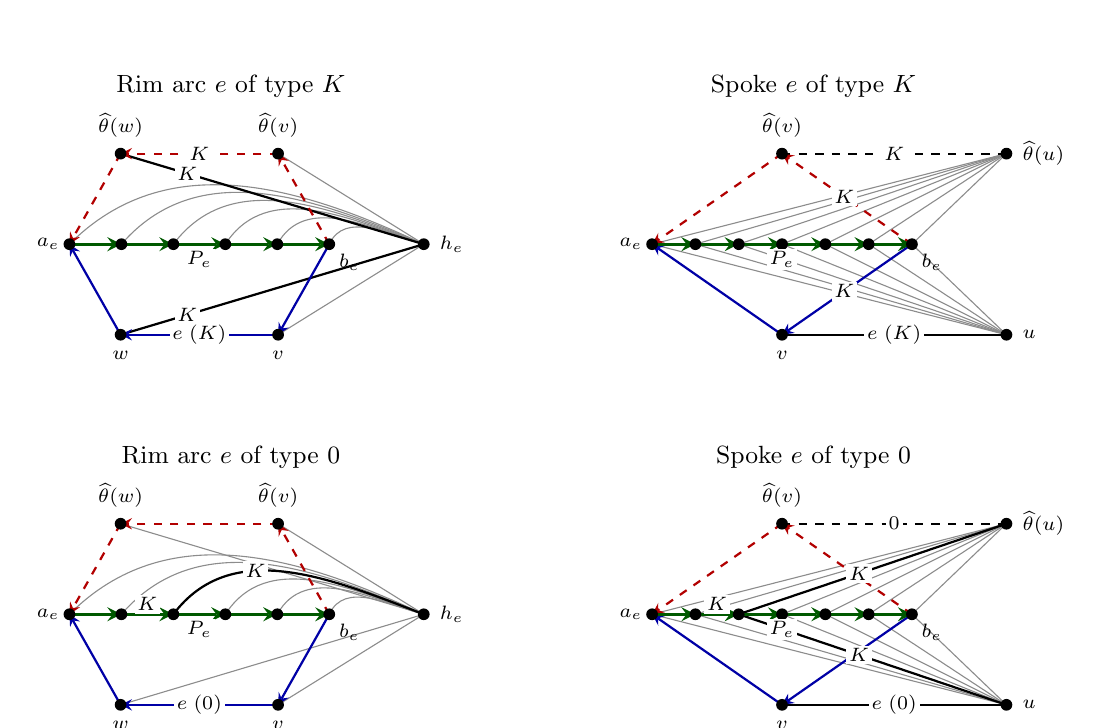
\begin{tikzpicture}[x=1cm,y=1cm,font=\small,>=stealth,
 dot/.style={circle,fill=black,inner sep=1.5pt},
 first/.style={blue!65!black,thick},
 second/.style={red!70!black,thick,dashed},
 shared/.style={green!35!black,very thick},
 spoke/.style={black!45,thin},
 tag/.style={fill=white,inner sep=1pt,font=\scriptsize}]
\begin{scope}[shift={(0.0,-0.0)},font=\scriptsize]
\coordinate (p0) at (-1.6500,0);
\coordinate (p1) at (-0.9900,0);
\coordinate (p2) at (-0.3300,0);
\coordinate (p3) at (0.3300,0);
\coordinate (p4) at (0.9900,0);
\coordinate (p5) at (1.6500,0);
\coordinate (v) at (1,-1.15); \coordinate (w) at (-1,-1.15);
\coordinate (vp) at (1,1.15); \coordinate (wp) at (-1,1.15);
\coordinate (h) at (2.85,0);
\draw[spoke] (p0) to[out=45,in=155] (h);
\draw[spoke] (p1) to[out=49,in=157] (h);
\draw[spoke] (p2) to[out=53,in=159] (h);
\draw[spoke] (p3) to[out=57,in=161] (h);
\draw[spoke] (p4) to[out=61,in=163] (h);
\draw[spoke] (p5) to[out=65,in=165] (h);
\draw[spoke] (v)--(h);
\draw[spoke] (w)--(h);
\draw[spoke] (vp)--(h);
\draw[spoke] (wp)--(h);
\draw[black,thick] (w)--(h); \draw[black,thick] (wp)--(h);
\path (w)--(h) node[tag,pos=.22] {$K$}; \path (wp)--(h) node[tag,pos=.22] {$K$};
\draw[first,->] (v)--(w);
\draw[first,->] (w)--(p0);
\draw[first,->] (p5)--(v);
\draw[second,->] (vp)--(wp);
\draw[second,->] (wp)--(p0);
\draw[second,->] (p5)--(vp);
\node[dot,label=right:$h_e$] at (h) {};
\node[dot,label=below:$ v $] at (v) {};
\node[dot,label=below:$ w $] at (w) {};
\node[dot,label=above:$ \widehat\theta(v) $] at (vp) {};
\node[dot,label=above:$ \widehat\theta(w) $] at (wp) {};
\path (v)--(w) node[tag,midway] {$ e\;(K) $};
\path (vp)--(wp) node[tag,midway] {$K$};
\draw[shared,->] (p0)--(p1);
\draw[shared,->] (p1)--(p2);
\draw[shared,->] (p2)--(p3);
\draw[shared,->] (p3)--(p4);
\draw[shared,->] (p4)--(p5);
\node[dot] at (p0) {};
\node[dot] at (p1) {};
\node[dot] at (p2) {};
\node[dot] at (p3) {};
\node[dot] at (p4) {};
\node[dot] at (p5) {};
\node[left] at (p0) {$a_e$};\node[below right] at (p5) {$b_e$};
\node[tag,below] at (0,-.05) {$P_e$};
\end{scope}
\node at (0.4,2.0) {Rim arc $e$ of type $K$};
\begin{scope}[shift={(7.4,-0.0)},font=\scriptsize]
\coordinate (p0) at (-1.6500,0);
\coordinate (p1) at (-1.1000,0);
\coordinate (p2) at (-0.5500,0);
\coordinate (p3) at (-0.0000,0);
\coordinate (p4) at (0.5500,0);
\coordinate (p5) at (1.1000,0);
\coordinate (p6) at (1.6500,0);
\coordinate (v) at (0,-1.15); \coordinate (vp) at (0,1.15);
\coordinate (h) at (2.85,-1.15); \coordinate (hp) at (2.85,1.15);
\draw[spoke] (p0)--(h);
\draw[spoke] (p0)--(hp);
\draw[spoke] (p1)--(h);
\draw[spoke] (p1)--(hp);
\draw[spoke] (p2)--(h);
\draw[spoke] (p2)--(hp);
\draw[spoke] (p3)--(h);
\draw[spoke] (p3)--(hp);
\draw[spoke] (p4)--(h);
\draw[spoke] (p4)--(hp);
\draw[spoke] (p5)--(h);
\draw[spoke] (p5)--(hp);
\draw[spoke] (p6)--(h);
\draw[spoke] (p6)--(hp);
\draw[black,thick] (v)--(h);\draw[black,thick,dashed] (vp)--(hp);
\draw[first,->] (v)--(p0);
\draw[first,->] (p6)--(v);
\draw[second,->] (vp)--(p0);
\draw[second,->] (p6)--(vp);
\node[dot,label=below:$ v $] at (v) {};
\node[dot,label=above:$ \widehat\theta(v) $] at (vp) {};
\node[dot,label=right:$ u $] at (h) {};
\node[dot,label=right:$ \widehat\theta(u) $] at (hp) {};
\path (v)--(h) node[tag,midway] {$e\;(K)$};
\path (vp)--(hp) node[tag,midway] {$ K $};
\path (p6)--(v) node[tag,pos=.52] {$K$};
\path (p6)--(vp) node[tag,pos=.52] {$K$};
\draw[shared,->] (p0)--(p1);
\draw[shared,->] (p1)--(p2);
\draw[shared,->] (p2)--(p3);
\draw[shared,->] (p3)--(p4);
\draw[shared,->] (p4)--(p5);
\draw[shared,->] (p5)--(p6);
\node[dot] at (p0) {};
\node[dot] at (p1) {};
\node[dot] at (p2) {};
\node[dot] at (p3) {};
\node[dot] at (p4) {};
\node[dot] at (p5) {};
\node[dot] at (p6) {};
\node[left] at (p0) {$a_e$};\node[below right] at (p6) {$b_e$};
\node[tag,below] at (0,-.05) {$P_e$};
\end{scope}
\node at (7.800000000000001,2.0) {Spoke $e$ of type $K$};
\begin{scope}[shift={(0.0,-4.7)},font=\scriptsize]
\coordinate (p0) at (-1.6500,0);
\coordinate (p1) at (-0.9900,0);
\coordinate (p2) at (-0.3300,0);
\coordinate (p3) at (0.3300,0);
\coordinate (p4) at (0.9900,0);
\coordinate (p5) at (1.6500,0);
\coordinate (v) at (1,-1.15); \coordinate (w) at (-1,-1.15);
\coordinate (vp) at (1,1.15); \coordinate (wp) at (-1,1.15);
\coordinate (h) at (2.85,0);
\draw[spoke] (p0) to[out=45,in=155] (h);
\draw[spoke] (p1) to[out=49,in=157] (h);
\draw[spoke] (p2) to[out=53,in=159] (h);
\draw[spoke] (p3) to[out=57,in=161] (h);
\draw[spoke] (p4) to[out=61,in=163] (h);
\draw[spoke] (p5) to[out=65,in=165] (h);
\draw[spoke] (v)--(h);
\draw[spoke] (w)--(h);
\draw[spoke] (vp)--(h);
\draw[spoke] (wp)--(h);
\draw[black,thick] (p2) to[out=53,in=159] (h);
\path (p2) to[out=53,in=159] node[tag,pos=.38] {$K$} (h);
\draw[first,->] (v)--(w);
\draw[first,->] (w)--(p0);
\draw[first,->] (p5)--(v);
\draw[second,->] (vp)--(wp);
\draw[second,->] (wp)--(p0);
\draw[second,->] (p5)--(vp);
\node[dot,label=right:$h_e$] at (h) {};
\node[dot,label=below:$ v $] at (v) {};
\node[dot,label=below:$ w $] at (w) {};
\node[dot,label=above:$ \widehat\theta(v) $] at (vp) {};
\node[dot,label=above:$ \widehat\theta(w) $] at (wp) {};
\path (v)--(w) node[tag,midway] {$ e\;(0) $};
\draw[shared,->] (p0)--(p1);
\draw[shared,->] (p1)--(p2);
\path (p1)--(p2) node[tag,above,midway] {$K$};
\draw[shared,->] (p2)--(p3);
\draw[shared,->] (p3)--(p4);
\draw[shared,->] (p4)--(p5);
\node[dot] at (p0) {};
\node[dot] at (p1) {};
\node[dot] at (p2) {};
\node[dot] at (p3) {};
\node[dot] at (p4) {};
\node[dot] at (p5) {};
\node[left] at (p0) {$a_e$};\node[below right] at (p5) {$b_e$};
\node[tag,below] at (0,-.05) {$P_e$};
\end{scope}
\node at (0.4,-2.7) {Rim arc $e$ of type $0$};
\begin{scope}[shift={(7.4,-4.7)},font=\scriptsize]
\coordinate (p0) at (-1.6500,0);
\coordinate (p1) at (-1.1000,0);
\coordinate (p2) at (-0.5500,0);
\coordinate (p3) at (-0.0000,0);
\coordinate (p4) at (0.5500,0);
\coordinate (p5) at (1.1000,0);
\coordinate (p6) at (1.6500,0);
\coordinate (v) at (0,-1.15); \coordinate (vp) at (0,1.15);
\coordinate (h) at (2.85,-1.15); \coordinate (hp) at (2.85,1.15);
\draw[spoke] (p0)--(h);
\draw[spoke] (p0)--(hp);
\draw[spoke] (p1)--(h);
\draw[spoke] (p1)--(hp);
\draw[spoke] (p2)--(h);
\draw[spoke] (p2)--(hp);
\draw[spoke] (p3)--(h);
\draw[spoke] (p3)--(hp);
\draw[spoke] (p4)--(h);
\draw[spoke] (p4)--(hp);
\draw[spoke] (p5)--(h);
\draw[spoke] (p5)--(hp);
\draw[spoke] (p6)--(h);
\draw[spoke] (p6)--(hp);
\draw[black,thick] (v)--(h);\draw[black,thick,dashed] (vp)--(hp);
\draw[first,->] (v)--(p0);
\draw[first,->] (p6)--(v);
\draw[second,->] (vp)--(p0);
\draw[second,->] (p6)--(vp);
\node[dot,label=below:$ v $] at (v) {};
\node[dot,label=above:$ \widehat\theta(v) $] at (vp) {};
\node[dot,label=right:$ u $] at (h) {};
\node[dot,label=right:$ \widehat\theta(u) $] at (hp) {};
\path (v)--(h) node[tag,midway] {$e\;(0)$};
\path (vp)--(hp) node[tag,midway] {$ 0 $};
\draw[black,thick] (p2)--(h) node[tag,pos=.45] {$K$};
\draw[black,thick] (p2)--(hp) node[tag,pos=.45] {$K$};
\draw[shared,->] (p0)--(p1);
\draw[shared,->] (p1)--(p2);
\path (p1)--(p2) node[tag,above,midway] {$K$};
\draw[shared,->] (p2)--(p3);
\draw[shared,->] (p3)--(p4);
\draw[shared,->] (p4)--(p5);
\draw[shared,->] (p5)--(p6);
\node[dot] at (p0) {};
\node[dot] at (p1) {};
\node[dot] at (p2) {};
\node[dot] at (p3) {};
\node[dot] at (p4) {};
\node[dot] at (p5) {};
\node[dot] at (p6) {};
\node[left] at (p0) {$a_e$};\node[below right] at (p6) {$b_e$};
\node[tag,below] at (0,-.05) {$P_e$};
\end{scope}
\node at (7.800000000000001,-2.7) {Spoke $e$ of type $0$};

\end{tikzpicture}
\caption{Wheel pairs for the marked transformer, with $c=8$.
The solid blue and dashed red auxiliary rims share the path $P_e$,
of length $c-3$ for a rim arc and $c-2$ for a spoke.
Arcs and spokes labeled $K$ are marked, and all others have type $0$.}
\label{fig:marked:transformer-wheel-pairs}
\end{figure}


An attachment vertex joined by an arc from $v$ and
$\widehat\theta(v)$ lies in
$N_{R^0}^+(v)\cap N_{R^0}^+(\widehat\theta(v))$.
An attachment vertex with arcs to these two roots lies in
$N_{R^j}^-(v)\cap N_{R^j}^-(\widehat\theta(v))$,
where $j=K$ precisely when $e\in E(H_\Lambda^K)$ and $j=0$ otherwise.
For $e=vu\in E(H_\Lambda)$, both attachment vertices of $P_e$
also lie in $N_{H^0}(u)\cap N_{H^0}(\widehat\theta(u))$.
If $P_e$ has an internal marked head, that vertex lies in
$N_{H^K}(u)\cap N_{H^K}(\widehat\theta(u))$.
The other internal labels have unmarked spokes to these two hubs.
For $e\in E(R_\Lambda)$, the hub $h_e$ is chosen after embedding $P_e$.
Each two-arc choice uses an intersection in
\eqref{eq:marked:absorber-row-patterns}; every other choice of a rim vertex
has at most one prescribed arc. All have at most two prescribed
spokes. If an attachment vertex $z$ has prescribed type-$K$ arcs
to $v$ and $\widehat\theta(v)$, their physical edges are
$\{z,\pi(v)\}$ and $\{z,\pi(\widehat\theta(v))\}$.
These edges are distinct because $v\ne\widehat\theta(v)$ and $\pi$ is injective. Pairwise separation of all rim vertices within either root graph is not required.

To embed each path $P_e$, write it as $z_0\cdots z_\ell$, with
the two attachment vertices fixed. Here $\ell=c-3\ge5$ for
$e\in E(R_\Lambda)$ and $\ell=c-2\ge6$ for $e\in E(H_\Lambda)$.
When the path requires a type-$K$ arc, we choose
$z_1\to z_2\in E(R^K)$ and all its other arcs in $R^0$.
We choose $z_1,\ldots,z_{\ell-2}$ successively, using one prescribed
arc and the specified spoke types, and choose $z_{\ell-1}$ in
$N_{R^0}^+(z_{\ell-2})\cap N_{R^0}^-(z_\ell)$ with unmarked spokes
to the prescribed hubs, if any.
Since $\ell\ge5$, the last free position $z_{\ell-1}$ differs
from the marked-head position $z_2$. All new labels avoid the
forbidden sets and are $(3d,\pi)$-separated from the roots and one another.

\paragraph{Step 3: Attachment pairings and common-neighborhood factors.}
For $v\in V_\Lambda$, the paths $P_e=(a_e,\ldots,b_e)$ give
the attachment sets
\begin{equation*}
\begin{aligned}
 A_v^+&:=\{a_e:e=w\to v\in E(R_\Lambda)\},&
 A_v^-&:=\{b_e:e=v\to w\in E(R_\Lambda)\},\\
 B_v^+&:=\{a_e:e=vu\in E(H_\Lambda)\},&
 B_v^-&:=\{b_e:e=vu\in E(H_\Lambda)\}.
\end{aligned}
\end{equation*}
Each set has size $s_v$. The vertices in $A_v^+\cup B_v^+$ are
joined by outgoing arcs from both $v$ and $\widehat\theta(v)$,
and those in $A_v^-\cup B_v^-$ have arcs into both roots.
Exactly $k_v$ of the arcs from $B_v^-$ into each root are marked.
We pair $A_v^+$ with $B_v^-$ and $B_v^+$ with $A_v^-$.
For each pair we construct two wheels, one through $v$ and one
through $\widehat\theta(v)$, sharing a hub. We assign to the pair one of
the $2s_v$ occurrences of $h_e$ indexed by auxiliary arcs $e$
of $\Lambda$ incident with $v$.
The vertex $h_e$ may not be assigned to the attachment vertex
of its own path, since that pair is already a spoke of $W_e$.

Exactly $k_v$ of these occurrences of $h_e$ require
the spoke $vh_e$ to have type $K$: those belonging to
marked arcs entering $v$.
We assign these occurrences to distinct attachment vertices of $A_v^+$
other than their own, and pair those attachment vertices with
the vertices $b_e\in B_v^-$ corresponding to type-$K$ spokes
$e=vu$ of $\Lambda$.
For this assignment, the left class consists of the $k_v$
occurrences corresponding to marked arcs entering $v$, and the
right class is $A_v^+$. Each occurrence is adjacent to every
vertex except the attachment vertex of its own path.
The forbidden pairs form a matching. Since $k_v\le s_v$,
Hall's condition can fail only when $s_v=k_v=1$, which Step~1
has excluded.
For the remaining assignment, the left class consists of the other
$2s_v-k_v$ occurrences and the right class of the unused vertices
in $A_v^+\cup A_v^-$. Again the forbidden pairs form a matching.
Both classes have size $2s_v-k_v\ge2$, so Hall's condition holds.
Hall's theorem (Theorem~\ref{thm:prelim:hall}) gives both assignments.
The remaining vertices of $A_v^+$ are paired with the remaining
vertices of $B_v^-$, which correspond to type-$0$ spokes $e=vu$ of
$\Lambda$. We pair $A_v^-$ with $B_v^+$ arbitrarily.

We then choose distinct hubs $h_e\in W$.
The spokes of $h_e$ to the rims of $W_e,W'_e$ have the types
specified above. Its spokes to the four attachment vertices
assigned at the two endpoints of $e$ have type $0$.
These attachment vertices are not vertices of their own
edge paths, so no two prescriptions conflict.
The only new vertices of $W$ with several prescribed neighbors
among the rim vertices of $\Lambda\cup\Lambda'$ are the hubs $h_e$
indexed by auxiliary arcs of $\Lambda$.
For $e=v\to w$, these prescribed neighbors belong to
$\{v,w,\widehat\theta(v),\widehat\theta(w)\}$.
The first two are $(3d,\pi)$-separated because they are endpoints
of an arc in $\Lambda$, the last two because they are
endpoints of its image in $\Lambda^{\prime}$, and all pairs crossing
the two sets are $(3d,\pi)$-separated by the assumed separation
between the two root sets. The additional neighbors
prescribed at $h_e$ are free path labels, all chosen
$(3d,\pi)$-separated. Thus all prescribed neighbors of $h_e$ are $(3d,\pi)$-separated,
as required by the hub-neighborhood lower bound in
\ref{item:marked-relative-absorber:typicality}. A hub used for a wheel
attached in Step~1 or in the construction of $\Lambda_{\rm att}$ has
at most one old root, so its prescribed rim vertices are also separated.
Each $h_e$ has prescribed spokes to $c+2$ labels from the rims
of $W_e,W'_e$ and to four further attachment labels.
If the root arc $e$ has type $0$, exactly one of these spokes
has type $K$ and $c+5$ have type $0$.
If $e$ has type $K$, exactly two have type $K$ and $c+4$ have type $0$.
These are precisely the two maximal cardinalities allowed in
\eqref{eq:marked:absorber-hub-input}, which supplies distinct unused hubs.

For each assigned pair of attachment vertices at $v$, we choose a
directed path of length $c-2$ from the outgoing attachment vertex to
the incoming attachment vertex, with new internal vertices.
Let $h$ be its assigned hub. If the prescribed arc from
the incoming attachment vertex to $v$ has type $K$, every new path
arc and every spoke from an internal path vertex to $h$ has type $0$.
Otherwise one internal path arc is marked, the spoke from its
head to $h$ has type $K$, and every other new spoke to $h$ has type $0$.
This gives two wheels, closed at $v$ and at $\widehat\theta(v)$,
with identical types on their shared edges.
We use the embedding order for the paths $P_e$, with $\ell=c-2$.
Each new internal label has one prescribed spoke at $h$.
The final two-edge connection is unmarked.
Let $\mathcal W_E:=\{W_e:e\in E(\Lambda)\}$ and
$\mathcal W'_E:=\{W'_e:e\in E(\Lambda)\}$. Let $\mathcal W_V$ and
$\mathcal W'_V$ be the indexed families of the wheels just
constructed for the assigned pairs, closed at $v$ and
$\widehat\theta(v)$, respectively, with one wheel for each assigned
pair at each $v\in V_\Lambda$.

For each $u\in U_\Lambda$, let $Z_u$ contain all vertices of the
paths indexed by the spokes of $\Lambda$ incident with $u$.
Its size is $|Z_u|=(c-1)d_{H_\Lambda}(u)$.
The number of $z\in Z_u$ for which $zu,z\widehat\theta(u)$ have type $K$
is the number of type-$0$ spokes of $\Lambda$ at $u$, namely
$(c-1)d_{H_\Lambda^K}(u)=|Z_u|/c$.
Every other vertex of $Z_u$ has type-$0$ spokes to both $u$
and $\widehat\theta(u)$.
The sets $Z_u$ are disjoint.
\paragraph{Two factors in the common neighborhood of $u,\widehat\theta(u)$.}
Fix $u\in U_\Lambda$ and put $u':=\widehat\theta(u)$.
The set $Z_u$ is $(3d,\pi)$-separated and avoids
$I_V\cup X_{\rm ex}$.

We apply Claim~\ref{clm:marked:balanced-common-neighbourhoods} with
$\eta=\eta_{\rm cl}/2$, $Z=Z_u$, $(c-1)r_1$ in place of $f$,
and the common $q,\phi$ and selector
$\kappa^{u,u'}$ supplied by \ref{item:marked-relative-absorber:common}.
For $I$ take $I_V$ together with all previously used rim vertices
outside $Z_u$. Their number is at most $\epsilon_*n+M+m_0$,
which is at most $\epsilon_{\rm bal}n$ for sufficiently large $n$.
The claim gives $A,B_1$. Put
$\mathcal C:=\mathcal C_{\mathcal Q}(u,u';A,B_1)$ and
$\psi:=\phi|_{\mathcal C}$.
Put $k:=|A|$. The bounds $an\le k\le n$ give $B_{\omega}^{-1}a^{c-1}k^{1-c}\le\psi(C)\le B_{\omega}k^{1-c}$.
For every $X\in\mathcal R_{c-1}(A,B_1)$, we also have
$|\mathcal A_{\mathcal C}(X)|\ge ak^{c^2}$.

Let $D_R$ consist of the physical rim edges in $F_{\rm ex}$ and
all physical rim edges used earlier in the construction. Put
\begin{equation*}
 \mathcal C^\circ:=\{C\in\mathcal C:E_{\rm phys}(C)\cap D_R=\varnothing\},
 \qquad \psi^\circ:=\psi|_{\mathcal C^\circ}.
\end{equation*}
Physical injectivity assigns at most one auxiliary arc to each
edge of $D_R$. At each $v\in A\cup B_1$, deleting these cycles
removes weight at most $C_{\rm ex}/n$. Each constituent cycle
of a paired absorber contains at most one prescribed root, so
a forbidden rim edge fixes at least one free vertex.
Consequently at most $C_{\rm ex}n^{c^2-1}$ absorbers of any fixed
root set are lost. Here, $C_{\rm ex}$ depends only on the fixed
parameters, $b_{\rm ex}$ and $M$. Since $k\ge an$, we may increase
$n_0$ so that
\begin{equation*}
 C_{\rm ex}/n\le\eta_{\rm cl}/2,\qquad
 C_{\rm ex}n^{c^2-1}\le(a/2)k^{c^2}.
\end{equation*}
Thus $\psi^\circ$ has vertex-sum error at most $\eta_{\rm cl}$,
and $|\mathcal A_{\mathcal C^\circ}(X)|\ge(a/2)k^{c^2}$ for
every $X\in\mathcal R_{c-1}(A,B_1)$.

The classes $A,B_1$ remain fixed. The spokes from $Z_u$ to $u,u'$
were prescribed by the paths $P_e$ and avoid $F_{\rm ex}$.

We apply Theorem~\ref{thm:simp:profile-finite-cleanup} to
$(\mathcal C^\circ,\psi^\circ)$ with classes $(A,B_1)$, scale $k$,
multiplicities $(1,c-1)$, multiplicity bound
$J_c$, coefficient bound $B_{\omega} a^{1-c}$ and absorber
coefficient $a/2$. We use the error $\eta_{\rm cl}$ and $q=r_1$.
Indeed, $|Z_u\cap A|=|Z_u|/c\le r_1$ and
$|Z_u\cap B_1|=(c-1)|Z_u\cap A|$. The new vertices returned by the
theorem must avoid the rim endpoints of forbidden spokes at $u,u'$
and all previously used rim vertices. We therefore use the forbidden set
\begin{equation*}
 (A\cup B_1)\cap
 \bigl((X_{\rm ex}\cap V)\cup X_{\rm spoke}
       \cup N_{\pi,3d}[(V(L_1\cup L_2)\cap V)\cup Z_u\cup X_{\rm old}]\bigr),
\end{equation*}
where $X_{\rm old}$ is the set of rim vertices used earlier,
$X_{\rm spoke}:=\{z\in A\cup B_1:zu\in F_{\rm ex}
\text{ or }zu'\in F_{\rm ex}\}$, and $N_{\pi,3d}[S]:= \{x\in V:\operatorname{dist}_\pi(x,z)\le3d \text{ for some }z\in S\}$. The forbidden set has size at most
$|X_{\rm ex}\cap V|+|X_{\rm spoke}|+ (6d+1)\bigl(|V(L_1\cup L_2)\cap V|+|Z_u|+|X_{\rm old}|\bigr)$, which is
bounded in terms of $c,d,M,m_0,f$. We use
$F_{\pi,3d}[A\cup B_1]$ as the separation graph, whose maximum
degree is at most $6d$.
The theorem gives edge-disjoint directed $C_c$-factors
$D_u^2,D_u^1\subseteq\mathcal C^\circ$ on $S_u,S_u\cup Z_u$,
respectively, where $|S_u|=ct_{\rm cl}$ and
$|V(C)\cap Z_u|\le1$ for every $C\in D_u^1$. Their cycles have one label in $A$ and $c-1$ in $B_1$,
with the marked arc entering the label in $A$. The common spoke types
are $K$ on $A$ and $0$ on $B_1$. The choice of $X_{\rm spoke}$ ensures
that the spokes at new labels avoid the forbidden physical edges.
Since the factors consist of auxiliary arcs of
$\mathcal Q$, their physical images are disjoint by physical
injectivity. The vertices of $S_u$ are $(3d,\pi)$-separated from the
rim vertices of $L_1\cup L_2$ and from all earlier choices.

For $i=1,2$, define the marked wheel families
\begin{equation*}
 B_u^i:=\{W(C,u):C\in D_u^i\},\qquad
 B_u^{\prime i}:=\{W(C,u'):C\in D_u^i\}.
\end{equation*}
Every cycle in either factor has the required spokes at both hubs.
Perform these choices successively for all $u\in U_\Lambda$, adding
the vertices and physical edges just used to the bounded exclusions.

\paragraph{Step 4: Verifying the two wheel decompositions.}
We work in the vector space whose coordinates are the typed rim-arc
and spoke occurrences of $\mathcal Q$. Write $\chi_X$ for the
edge-indicator vector of a typed extended graph $X$ and $\ind_e$ for
the unit vector at an edge occurrence $e$. For an indexed wheel
family $\mathcal F$, let $\chi_{\mathcal F}:=\sum_{W\in\mathcal F}\chi_W$.
The attachments at each root in $V_\Lambda$ are paired
once, in their specified direction and type,
and every occurrence of $h_e$ at an endpoint of an auxiliary arc $e$ of $\Lambda$ is assigned once.
Consequently
\begin{equation*}
 \chi_{\mathcal W_E}-\chi_{\mathcal W'_E}-(\chi_{\mathcal W_V}-\chi_{\mathcal W'_V})
 =\chi_\Lambda-\chi_{\Lambda'}+
   \sum_u\sum_{z\in Z_u}
       \left(\ind_{zu}-\ind_{z\widehat\theta(u)}\right).
\end{equation*}
Each spoke in the last sum has its already specified common type
at $u$ and $\widehat\theta(u)$. The vector
$\chi_{B_u^1}+\chi_{B_u^{\prime2}}-\chi_{B_u^{\prime1}}-\chi_{B_u^2}$ equals
$\sum_{z\in Z_u}(\ind_{zu}-\ind_{z\widehat\theta(u)})$.
Thus the indexed wheel families
\begin{equation*}
 \mathcal M:=\mathcal W_E\cup\mathcal W'_V\cup\bigcup_u(B_u^{\prime1}\cup B_u^2),
 \qquad
 \mathcal M':=\mathcal W'_E\cup\mathcal W_V\cup\bigcup_u(B_u^1\cup B_u^{\prime2})
\end{equation*}
satisfy $\chi_{\mathcal M}-\chi_{\mathcal M'}=\chi_\Lambda-\chi_{\Lambda'}$.

We first check that no auxiliary arc or spoke is repeated within
either $\mathcal M$ or $\mathcal M'$.
The paths $P_e$ have pairwise disjoint vertex sets, and the
internal vertices of every subsequently constructed path are new.
In $\mathcal M$, the wheels in $\mathcal W'_V$ close at
$\widehat\theta(v)$, whereas those in $\mathcal W_E$ use roots in
$\Lambda$. In $\mathcal M'$, the wheels in $\mathcal W_V$ close at
$v$, and those in $\mathcal W'_E$ use roots in $\Lambda'$.
The assignment at $h_e$ excludes the attachment vertex of its own
path, so no attachment spoke is repeated. The remaining new auxiliary arcs and spokes of
the wheels in $\mathcal W_V,\mathcal W'_V$ have a rim endpoint among
the internal vertices of the paths constructed for the assigned pairs.
These vertices were chosen outside the earlier rim vertices.
On $Z_u$, the wheels in $B_u^{\prime1}$ use spokes at
$\widehat\theta(u)$, while the corresponding wheels in $\mathcal W_E$
use spokes at $u$. In $\mathcal M'$, $B_u^1$ uses $u$
and $\mathcal W'_E$ uses $\widehat\theta(u)$.
All other edges of the factor-wheel families meet $S_u$.
The factors $D_u^1,D_u^2$ are edge-disjoint and have no edge
inside $Z_u$. Identifying vertices under $\widehat\theta$ does not
repeat an auxiliary edge, since the free path sets and the sets $S_u$ are disjoint. The two endpoints of any
auxiliary arc of $\Lambda$ still have distinct images.
Physical injectivity of $\mathcal Q$ gives distinct physical images
to distinct rim arcs, including arcs of different types. Spokes retain
their endpoints and belong to a simple bipartite graph on $V,W$.
Their physical images are distinct from all rim edges.
Thus each of $\mathcal M,\mathcal M'$ is a packing, and the auxiliary
edge partitions give physical edge partitions. Consequently
$T^+:=(\bigcup\mathcal M)-\Lambda=(\bigcup\mathcal M')-\Lambda'$
is physically edge-disjoint from both $\Lambda$ and $\Lambda'$.
Set $T:=T^+\cup P_1\cup P_2$. Then
\begin{equation*}
 L_1\cup T=(\Lambda\cup T^+)\cup P_2,\qquad
 L_2\cup T=(\Lambda'\cup T^+)\cup P_1.
\end{equation*}
These are edge-disjoint unions of decomposable graphs.
All new edges have a new endpoint, and all physical edges of $T$
avoid $F_{\rm ex}$ and the original root graphs. The number of
new labels fits the bound used in the choice of $M$, independently
of the bounded exclusions. This proves the Claim.
\end{proof}

\paragraph{Embedding the five graphs and assembling the absorber.}
For the given $L$, we embed the five graphs of
\eqref{eq:marked:four-maps} using the bounds for choosing rim
vertices and hubs. New vertices avoid $I_V\cup I_W\cup I_0$ and
previously used vertices. New physical edges avoid
$E_{\rm phys}(L)\cup F_0$ and previously used physical edges.
The following embeddings allow us to apply
Claim~\ref{clm:marked:close-root-transformer} to the four maps.
For $j\in\{0,K\}$, to embed the expansion of a type-$j$ arc
$x\to y$, which need not belong to $R^j$, we choose
$y'\in N_{R^j}^+(x)$ and then
$x'\in N_{R^j}^-(y)\cap N_{R^j}^-(y')$, subject to the exclusions above.
For $j=K$, the last two arcs have distinct physical images
$\{x',\pi(y)\}$ and $\{x',\pi(y')\}$, since $y\ne y'$.
We complete the remaining path of the new wheel as in Step~2,
with its final two arcs unmarked. An internal arc is marked precisely
when $j=0$. Its hub has one marked and $c-1$ unmarked prescribed
spokes on separated labels. The distinguished arc $x'\to y'$ is
deleted in the expansion, but is included among the two adjacency
requirements when choosing $x'$.

For a spoke expansion, we first choose $u'\in W$ so that $xu'$
has the type of the expanded spoke. We then choose $x'$ so that
$x'u,x'u'$ have this type, and complete a marked $c$-wheel at $u'$
through $x'$. Its marked head is $x'$ precisely when the expanded
spoke has type $K$.
Equation~\eqref{eq:marked:absorber-hub-input}, applied to the single
prescribed vertex $x$, supplies $u'$. Equation~\eqref{eq:marked:absorber-vertex-input},
with $B_R=V$ and prescribed hub set $\{u,u'\}$, then supplies
$x'$ with the required spoke type.
To complete a wheel through a fixed marked head $v$, we choose
its predecessor in $N_{R^K}^-(v)$ and its successor in $N_{R^0}^+(v)$.
We join the successor to the predecessor by a directed path of unmarked
arcs. Its last internal vertex is chosen in
$N_{R^0}^+(z)\cap N_{R^0}^-(w)$, where $z$ is the preceding vertex
and $w$ the fixed endpoint, subject to the prescribed spokes and exclusions.
When the spoke at $v$ has type $0$, we choose the predecessor in
$N_{R^0}^-(v)$ and the joining path with exactly one arc in $R^K$
and all its other arcs in $R^0$, including its final two arcs.
For a fixed hub, the prescribed spokes are marked at the marked head
and unmarked at all other rim vertices. Otherwise the hub is chosen last.
This also embeds the attached wheels, including those of Step~1.
Each new rim vertex is chosen from $B_R\cap N_{H^j}(J_{\rm hub})$,
where $J_{\rm hub}\subseteq W$ is the prescribed hub set,
$|J_{\rm hub}|\le2$, and $B_R$ is listed in
\eqref{eq:marked:absorber-row-patterns}, while maintaining
$(3d,\pi)$-separation from all earlier rim vertices.

Using these expansions, we embed $L'_{\rm exp},J'_{\rm exp}$
and $\Gamma$ on new roots. The original edges of $L',J'$ and
$\Gamma_0$ are deleted during expansion, so none is required to
belong to $\mathcal Q$. The five embedded graphs are vertex-disjoint.
Every arc $x\to y$ of $L$ satisfies
$\operatorname{dist}_\pi(x,y)>3d$, since $L\subseteq\mathcal Q$.
We choose all new rim vertices separated from the original roots and
from earlier choices. Each pair of graphs in an arrow then has
separated sets of rim vertices. The rim vertices of $L$ need not be pairwise
$(3d,\pi)$-separated. Let $\mathcal D$ be the union of the five graphs in
\eqref{eq:marked:four-maps}. We apply
Claim~\ref{clm:marked:close-root-transformer} to arrow $j$, for
$j=1,\ldots,4$, to obtain $T_j$, using
\begin{equation*}
X_{\rm ex}=I_0\cup V(\mathcal D)\cup\bigcup_{i<j}V(T_i),\qquad F_{\rm ex}=F_0\cup E_{\rm phys}(\mathcal D)
\cup\bigcup_{i<j}E_{\rm phys}(T_i).
\end{equation*}
All auxiliary vertices of $\mathcal D\cup\bigcup_{i<j}T_i$ lie in the
original root set together with at most $M$ new vertices. Its physical
endpoints lie among these labels and the successors of its rim vertices,
so there are at most $2(m_0+M)$ physical endpoints and at most
$4(m_0+M)^2$ physical edges.
Thus $|X_{\rm ex}|+|F_{\rm ex}|\le b_{\rm ex}$ at every application.
The transformers are edge-disjoint from one another and from
$\mathcal D$.
Set
\begin{equation*}
A_L:=(L_{\rm att}-L)\cup T_1\cup L'_{\rm exp}
       \cup T_2\cup\Gamma\cup T_3\cup J'_{\rm exp}
       \cup T_4\cup J_{\rm att}.
\end{equation*}
One decomposition groups these edges as
\begin{equation*}
L_{\rm att}-L,\quad T_1\cup L'_{\rm exp},
 \quad T_2\cup\Gamma,\quad
 T_3\cup J'_{\rm exp},\quad T_4\cup J_{\rm att}.
\end{equation*}
After adding $L$, the other decomposition
uses
\begin{equation*}
L_{\rm att}\cup T_1,\quad L'_{\rm exp}\cup T_2,
 \quad\Gamma\cup T_3,\quad
 J'_{\rm exp}\cup T_4,\quad J_{\rm att}.
\end{equation*}
Each group containing $T_j$ is decomposable by
Claim~\ref{clm:marked:close-root-transformer}.
The graphs $L_{\rm att}-L$ and $J_{\rm att}$ are unions of marked
$c$-wheels by construction. Among the five graphs,
only $L_{\rm att}$ meets the original roots, and its added edges have
new endpoints. Every transformer edge has an endpoint outside
$V(\mathcal D)$. Thus no edge of $A_L$ joins two original roots.

\end{proof}

\part{Exact completion by iterative absorption}
\label{part:completion}

\section{Completion after bounded changes}
We reserve one bounded absorber in the completion sample and decompose
every permitted divisible remainder using that same absorber.
The two propositions below are used in the preparation arguments of
Part~\ref{part:main-proof}.
Their proofs are given in Section~\ref{sec:completion:proof}.
For the ordinary and marked models, we first prove the corresponding
cover-down lemmas (Lemmas~\ref{lem:completion:ordinary-cover-down}
and~\ref{lem:completion:marked-cover-down}) and then iterate them along a vortex. The sampling estimates establish the hypotheses at
every level simultaneously, including all potential roots that may be
chosen later.

The completion samples are constructed from a graph $P$ on $V$, a
disjoint hub set $U$ and a permutation $\pi$ of $V$, with an integer
separation parameter $d\ge2$. Their joint distributions are specified in
Definitions~\ref{def:ordinary-local-reference} and~\ref{def:completion:marked-sample}.
In the ordinary sample, the rim is obtained by independent edge sampling
in $P$, retaining only edges $xy$ with $\operatorname{dist}_\pi(x,y)>3d$. Its untyped
spoke graph is formed from the raw interval and label variables,
independently of the rim sampling.
In the marked sample, each edge of $P$ is assigned at most one
direction and type, independently over these edges and independently
of the spoke construction. An edge directed from $x$ to $y$ gives
the auxiliary arc $x\to y$ in type $0$ and $x\to\pi^{-1}(y)$ in
type $K$. An auxiliary arc is retained precisely when its endpoints
have $\pi$-distance greater than $3d$.
The marked spokes join each hub to the vertices of its sampled
color-$1$ intervals. The unmarked spokes at a hub $u$ are precisely
the edges $xu$ for which $x\in V$ lies outside the extended intervals
of both colors at $u$ and has label $\mathrm o_1$.

For $v\in V$ and $u\in U$, the parameters $a_u,b_u$ are the
probabilities that $vu$ is assigned to approximate
packing as a type-$K$ or type-$0$ spoke, respectively.
These assignments use interval color $2$ and label color $\mathrm o_2$.
The completion construction uses the same raw interval and label
variables as the approximate-packing construction.

For ordinary extended graphs, $\Delta_*$ is the maximum degree of
the union of the rim and spoke graphs. For typed extended graphs,
it is the larger of the maximum auxiliary and physical incidence degrees.
Their symmetric differences are taken between arc and spoke occurrences,
with directions and types retained.

\subsection{Ordinary completion after bounded changes}
Let $P$ be a graph on $V$, let $U$ be disjoint from $V$, let $\pi$
be a permutation of $V$, and let $d\ge2$ be an integer.
An ordinary completion host $\mathcal Q=(V,U,R,H)$ has
$R\subseteq P$ with $\operatorname{dist}_\pi(x,y)>3d$ for every
$xy\in E(R)$, and $H$ is bipartite with parts $V,U$
(Definition~\ref{def:completion:ordinary-host}). For an integer $r\ge3$,
$\mathcal Q$ is $r$-wheel-divisible when $d_R(v)=2d_H(v)$ for every
$v\in V$ and $r\mid d_H(u)$ for every $u\in U$.

\begin{proposition}[Ordinary completion after bounded changes]
\label{prop:completion:ordinary-construction}
Let $r\ge3$ be an integer, let $\alpha_0,\epsilon_{\max}>0$,
and let $0<\varrho_*\le1$ and $0<s_*\le1/100$. Suppose that
\begin{equation}
 0<\zeta_{\rm rem}\ll\epsilon
 \ll\epsilon_{\max},\alpha_0,\varrho_*,s_*,1/r.
 \label{eq:completion:ordinary-input-hierarchy}
\end{equation}
Assume also $\epsilon\le\epsilon_{\max}$. For every pair of integers $d\ge2$,
$L_0\ge1$ and every $\chi\in(0,1)$, there are integers
$M_{\rm abs},n_0\ge1$ for which the following holds.

Let $P$ be a simple $D$-regular graph on $V$, where $|V|=n\ge n_0$,
$D$ is even and $D\ge(\delta_{C_r}+\alpha_0)n$.
Let $U$ be disjoint from $V$, let
$\varrho:=2|U|/D\in[\varrho_*,1]$, and let $s\in[s_*,1/100]$.
Let $a_u,b_u\ge0$ such that $a_u\le1/8$ and $s+b_u\le1-(1+1/d)a_u$ for all $u\in U$.

Then there are $I\subseteq V$, $J\subseteq U$ and a permutation
$\pi$ of $V$, all fixed before sampling, such that
$|I|=\lfloor\epsilon n\rfloor$, $|J|=\lfloor\epsilon|U|\rfloor$ and $\pi(I)=I$. Every cycle of $\pi$ has
length greater than
$\max\{10d,L_0\}$.
Let $\mathcal B$ be the ordinary completion sample on $(P,V,U,\pi)$
with parameters $\varrho,s,d,(a_u),(b_u)$.

With probability at least $1-\chi-n^{-12}$, there is an extended
subgraph $\mathcal A\subseteq\mathcal B$ on at most $M_{\rm abs}$
auxiliary vertices, with $\mathcal A[I\cup J]=\varnothing$, such that
every ordinary $r$-wheel-divisible completion host $\mathcal R$
on $(P,V,U,\pi)$ satisfying
\begin{equation}
 \mathcal A\subseteq\mathcal R,\qquad
 \mathcal R[I\cup J]=\mathcal B[I\cup J],\qquad
 \Delta_*\bigl((\mathcal R-\mathcal A)\triangle\mathcal B\bigr)
       \le\zeta_{\rm rem}n
 \label{item:completion:perturbation:ordinary}
\end{equation}
has an $r$-wheel decomposition.
\end{proposition}


\subsection{Marked completion after bounded changes}
Let $P$ be a graph on $V$, let $U$ be disjoint from $V$, let $\pi$
be a permutation of $V$, and let $d\ge2$ be an integer.
A marked completion host $\mathcal Q=(V,U,R^0,R^K,H^0,H^K)$
on $(P,V,U,\pi)$ with separation parameter $d$
(Definition~\ref{def:completion:marked-host}) has digraphs $R^0,R^K$
on $V$ and edge-disjoint bipartite graphs $H^0,H^K$ on $(V,U)$.
Every rim arc $x\to y$ satisfies $\operatorname{dist}_\pi(x,y)>3d$.
Its physical image is $\{x,y\}$ in type $0$ and $\{x,\pi(y)\}$ in
type $K$, and belongs to $E(P)$.
The spoke graphs satisfy
$N_{H^0}(u)\cap\pi(N_{H^K}(u))=\varnothing$ for every $u\in U$.
Write $R:=R^0\dot\cup R^K$ and $H:=H^0\dot\cup H^K$.
For an integer $c\ge3$, $\mathcal Q$ is marked $c$-wheel-divisible
when
\begin{equation*}
\begin{aligned}
 d_R^+(v)=d_R^-(v)&=d_H(v),\quad d_{R^K}^-(v)=d_{H^K}(v) &&(v\in V),\\
 d_{H^0}(u)&=(c-1)d_{H^K}(u) &&(u\in U).
\end{aligned}
\end{equation*}

\begin{proposition}[Marked completion after bounded changes]
\label{prop:completion:marked-construction}
Let $\alpha_0,\epsilon_{\max}>0$, $0<\varrho_*\le1$ and
$0<s_*\le1/100$.
There is an integer $c_0=c_0(\alpha_0,\varrho_*,s_*)\ge8$ such that,
for every even integer $c\ge c_0$, the following holds.
Suppose that
\begin{equation}
 0<\zeta_{\rm rem}\ll\epsilon
 \ll\epsilon_{\max},\alpha_0,\varrho_*,s_*,1/c.
 \label{eq:completion:marked-input-hierarchy}
\end{equation}
Assume also $\epsilon\le\epsilon_{\max}$. For every pair of integers $d\ge2$,
$L_0\ge1$ and every $\chi\in(0,1)$, there are integers
$M_{\rm abs},n_0\ge1$ for which the following holds.

Let $P$ be a simple $D$-regular graph on $V$, where $|V|=n\ge n_0$,
$D$ is even and $D\ge(1/2+\alpha_0)n$.
Let $U$ be disjoint from $V$, let
$\varrho:=2|U|/D\in[\varrho_*,1]$, and let $s\in[s_*,1/100]$.
Let $t:=s/(c-1)$ and let $a_u,b_u\ge0$ such that $t+a_u\le1/8$ and $s+b_u\le1-(1+1/d)(t+a_u)$ for all $u\in U$.

Then there are $I\subseteq V$, $J\subseteq U$ and a permutation
$\pi$ of $V$, all fixed before sampling, such that
$|I|=\lfloor\epsilon n\rfloor$, $|J|=\lfloor\epsilon|U|\rfloor$ and $\pi(I)=I$. Every cycle of $\pi$ has
length greater than
$\max\{10d,L_0,10(c+7)(3d+3)\}$.
Let $\mathcal B$ be the marked completion sample on $(P,V,U,\pi)$
with parameters $c,\varrho,s,d,(a_u),(b_u)$.

With probability at least $1-\chi-n^{-12}$, there is an extended
subgraph $\mathcal A\subseteq\mathcal B$ on at most $M_{\rm abs}$
auxiliary vertices, with $\mathcal A[I\cup J]=\varnothing$, such that
every physically injective, marked $c$-wheel-divisible
completion host $\mathcal R$ on $(P,V,U,\pi)$ satisfying
\begin{equation}
 \mathcal A\subseteq\mathcal R,\qquad
 \mathcal R[I\cup J]=\mathcal B[I\cup J],\qquad
 \Delta_*\bigl((\mathcal R-\mathcal A)\triangle\mathcal B\bigr)
       \le\zeta_{\rm rem}n
 \label{item:completion:perturbation:marked}
\end{equation}
has a marked $c$-wheel decomposition.
\end{proposition}




\subsection{Vortices on vertices and factor indices}
We carry out iterative absorption along a vortex consisting of nested
sets of rim vertices and hubs (see \cite{BKLO2016} and
\cite[Definition~3.6, Lemma~3.8 and the proof of Theorem~1.2]{BarberEtAl2020Minimalist}).
At each level, the hub set records the remaining factor indices, and
its size determines the target degree into the corresponding vertex set.
The sets are fixed before sampling the completion graph.
Section~\ref{sec:completion:proof} gives the probabilistic estimates
needed for the sampled rim and spoke graphs on these sets.

\begin{definition}[Vortex]\label{gls:vortex}
Let $\beta,\varrho_*>0$, $0<\epsilon<1/4$ and $m_*\in\mathbb N$.
Let $P$ be a $D$-regular graph on $V$, where $|V|=n\ge1$ and
$D\ge n/2$, and let $U$ be disjoint from $V$ with
$\varrho:=2|U|/D\in[\varrho_*,1]$.
A \emph{$(\beta,\epsilon,\varrho_*,m_*)$-vortex} for $(P,U)$ is a
pair of nested sequences
\begin{equation*}
 V=V_0\supseteq\cdots\supseteq V_\ell,\qquad
 U=U_0\supseteq\cdots\supseteq U_\ell
 \qquad(\ell\ge0).
\end{equation*}
With $n_i:=|V_i|$, $u_i:=|U_i|$ and $D_i:=2u_i/\varrho$,
these sequences satisfy the following conditions:
\begin{enumerate}[label=\textup{(V\arabic*)}]
\item
$n_{i+1}=\lfloor\epsilon n_i\rfloor$ for $0\le i<\ell$, and
$\epsilon m_*/2\le n_\ell<m_*$;
\item
$u_{i+1}=\lfloor\epsilon u_i\rfloor$ for $0\le i<\ell$;
\item
for $1\le i\le\ell$ and $v\in V_{\max\{0,i-2\}}$,
\begin{equation}
 D_i=\frac Dn n_i\pm \beta n_i,\qquad
 d_P(v;V_i)=\frac{2u_i}{\varrho}\pm \beta n_i.
 \label{eq:family:real-centres}
\end{equation}
\end{enumerate}
\end{definition}

\begin{lemma}
\label{lem:writing:nested-pairs}
Let $\beta,\varrho_*>0$ and $0<\epsilon<1/4$.
There is an integer $m_0$ such that the following holds for all
integers $n\ge m_*\ge m_0$.
Let $P$ be a $D$-regular graph on $V$, where $|V|=n$ and $D\ge n/2$,
and let $U$ be disjoint from $V$ with
$\varrho:=2|U|/D\in[\varrho_*,1]$.
Then $(P,U)$ admits a $(\beta,\epsilon,\varrho_*,m_*)$-vortex.
\end{lemma}
\begin{proof}
We choose $m_0$ sufficiently large in terms of $\beta,\epsilon,\varrho_*$.
Starting with $n_0:=n$ and $u_0:=|U|$, define
$n_{i+1}:=\lfloor\epsilon n_i\rfloor$ and
$u_{i+1}:=\lfloor\epsilon u_i\rfloor$, stopping at the first
$n_\ell<m_*$. Then
$n_\ell\ge\epsilon m_*-1\ge\epsilon m_*/2$.

We choose the sets $V_i$ successively. At step $i\in[\ell]$, sample a uniform
$n_i$-subset of $V_{i-1}$. For each
$v\in V_{\max\{0,i-2\}}$, the mean of $d_P(v;V_i)/n_i$ is
$d_P(v;V_{i-1})/n_{i-1}$, including when $v\notin V_{i-1}$.
Since $n_i\ge\epsilon n_{i-1}/2$,
the sampling concentration inequality (Lemma~\ref{lem:simp:product-sampling}),
with exchange bound $1/n_i$, gives
\begin{equation*}
 \Pr\left(
 \left|\frac{d_P(v;V_i)}{n_i}
       -\frac{d_P(v;V_{i-1})}{n_{i-1}}\right|
       >n_{i-1}^{-1/3}\right)
 \le 2\exp(-\epsilon n_{i-1}^{1/3}).
\end{equation*}
There are at most $2n_{i-1}/\epsilon$ possible roots
$v\in V_{\max\{0,i-2\}}$: for $i\ge2$, this follows from
$n_{i-2}<(n_{i-1}+1)/\epsilon$, while for $i=1$ there are $n_0$ roots.
For sufficiently large $m_0$, the union bound is less than one,
so a successful choice exists at every step. For $j\le i$, each
such $v$ also belongs to $V_{\max\{0,j-2\}}$. Its accumulated
normalized error is therefore at most
$\sum_{j=0}^{i-1}n_j^{-1/3} \le\frac{m_*^{-1/3}}{1-\epsilon^{1/3}}\le\frac\beta2$,
since $n_{j+1}\le\epsilon n_j$ and $n_{\ell-1}\ge m_*$.
Thus $d_P(v;V_i)=\frac Dn n_i\pm \frac\beta2 n_i$ for all $v\in V_{\max\{0,i-2\}}$.

We choose nested sets $U_i$ of sizes $u_i$. Put $a:=|U|/n$ and
$e_i:=u_i-a n_i$, so $e_0=0$ and $0<a\le1/2$.
Writing
$r_i:=\epsilon n_i-n_{i+1}$ and $s_i:=\epsilon u_i-u_{i+1}$,
we have $r_i,s_i\in[0,1)$ and
$e_{i+1}=\epsilon e_i+a r_i-s_i$. Hence
$|e_i|<\frac1{1-\epsilon}$ and $\left|\frac{2u_i}{\varrho}-\frac Dn n_i\right| <\frac{2}{(1-\epsilon)\varrho_*}<\frac3{\varrho_*}$.
We take $m_0$ large enough that
$3/\varrho_*\le\beta\epsilon m_0/4$.
Since $n_i\ge n_\ell\ge\epsilon m_*/2$, the last bound is at most
$\beta n_i/2$. Combining the two estimates gives
\eqref{eq:family:real-centres}.
\end{proof}

\Needspace{8\baselineskip}

\paragraph{Degrees on differences of vortex sets.}
For a vortex as above, set $V_{\ell+1}:=U_{\ell+1}:=\varnothing$.
If $0\le i<\ell$ and $(j,k)\in\{(i,i+2),(i+1,i+2)\}$, put
$A:=V_j\setminus V_k$, $B:=U_j\setminus U_k$ and
$D_A:=D_j-D_k=2|B|/\varrho$, with
$n_{\ell+1}:=u_{\ell+1}:=D_{\ell+1}:=0$.
Both level-$j$ and level-$k$ estimates in
\eqref{eq:family:real-centres} apply at every $v\in V_i$.
The estimates at level $0$ and at the empty level are exact.
Since $n_k\le\epsilon n_j$ and $|A|\ge(1-\epsilon)n_j$,
subtraction gives
\begin{equation}
 \left|D_A-\frac Dn|A|\right|,\quad
 |d_P(v;A)-D_A|\le\beta(n_j+n_k)\le\tfrac53\beta|A|
 \quad(v\in V_i).
 \label{eq:completion:vortex-differences:ordinary}
\end{equation}

\begin{lemma}
\label{lem:writing:shell-permutation}
Let $h\ge1$ and $t\ge0$ be integers, and let
$V=V_0\supseteq V_1\supseteq\cdots\supseteq V_t$ be finite sets.
Suppose every nonempty $V_i\setminus V_{i+1}$ and the terminal set
$V_t$ have at least $h$ elements. Then there is a permutation $\pi$ of
$V$, all of whose cycles have length at least $h$, such that
$\pi(V_i)=V_i$ for all $0\le i\le t$.
\end{lemma}
\begin{proof}
Put one cyclic permutation on each nonempty set
$V_i\setminus V_{i+1}$ and one on $V_t$. Their disjoint union has all
the asserted properties.
\end{proof}

\section{Ordinary cover-down}
Given an $r$-wheel-divisible ordinary completion host $\mathcal R$
satisfying the estimates below,
Lemma~\ref{lem:completion:ordinary-cover-down} produces a packing of
ordinary $r$-wheels that leaves an $r$-wheel-divisible remainder on $(I,J)$.
Writing $\mathcal R'$ for the remainder and
$\mathcal D:=\mathcal R[I\cup J]-\mathcal R'$, the bounds are
\begin{equation*}
 \Delta_*(\mathcal D)\le\gamma|I|,\qquad
 \Delta_*(\mathcal D\cap\operatorname{star}(T,W))\le\sigma|I|,
 \qquad \mathcal R'[T\cup W]=\mathcal R[T\cup W].
\end{equation*}
Here $\operatorname{star}(T,W)$ consists of all potential rim edges
and spokes incident with $T\cup W$, including those with their
other endpoint outside this set.
The proof of Proposition~\ref{prop:completion:ordinary-construction}
iterates this step along a vortex and absorbs the terminal remainder.

\subsection{Ordinary local cycle estimates}
In the local estimates, $A,B$ are summation domains and $X,Y$
contain the possible vertex and hub roots. These estimates are used
to construct the cycle factors and path extensions that cover boundary
edges. We use $0<\omega_{\rm est}\le1/8$ as a common lower bound
and $\omega_{\rm est}^{-1}$ as a coefficient upper bound.

\begin{definition}[Ordinary local cycle estimates]\label{gls:ordinary-local-cycle-estimates}
Let $r\ge3$, let $V,U$ be disjoint, let $P$ be a graph on $V$,
and let $\mathcal Q=(V,U,R,H)$ be an ordinary extended graph.
Let $A\subseteq X\subseteq V$ and $B\subseteq Y\subseteq U$ be nonempty,
and let $a:=|A|$, $D_A>0$, $q,s\in(0,1]$, $0<\omega_{\rm est}\le1/8$ and $\eta\ge0$.

Let $P_{\rm el}$ be a fixed subgraph with $R\subseteq P_{\rm el}\subseteq P$,
and let $F$ be a fixed exception graph on $V$.
Let $\lambda_A:\mathcal C_r(P[A])\to\mathbb R_{>0}$ be a
fractional $C_r$-decomposition with
$\omega_{\rm est}a^{2-r}\le\lambda_A(C)\le \omega_{\rm est}^{-1}a^{2-r}$.

The coefficients and sums in
\eqref{eq:loads:ordinary-coefficients}--\eqref{eq:loads:ordinary-neighbourhood}
are defined using this fixed $\lambda_A$. For each candidate cycle
$C$ through $v$, the corresponding summand in $Z^A_{v,\{u\}}$
contains the indicators of membership in $\mathcal Q$ for every
edge of the wheel with rim $C$ and hub $u$ except the root spoke $vu$.
The target $\ell^A_v$ is defined from $P,F,\lambda_A,D_A$ in
\eqref{eq:loads:ordinary-coefficients}.

For $r=3$ and each $x\in X$, let
$\lambda_{A,x}:E(P[N_P(x;A)])\to\mathbb R_{>0}$ be the perfect
fractional matching used in \eqref{eq:loads:triangular-endpoints},
with $\omega_{\rm est}/a\le\lambda_{A,x}(e)\le\omega_{\rm est}^{-1}/a$
for every $e\in E(P[N_P(x;A)])$. In this case, let $b:=|B|$,
$E_x:=N_P(x;A)\setminus N_F(x)$ and $\mathcal E_x:=E(P[E_x])\setminus E(F)$.
For $v\in E_x$ and $u\in B$, the triangle targets are
\begin{equation*}
 m_{x,v}:=\sum_{w:\,vw\in\mathcal E_x}\lambda_{A,x}(vw),\qquad
 m_{x,u}:=\frac{q}{bs}\sum_{vw\in\mathcal E_x}\lambda_{A,x}(vw),
\end{equation*}
where each unordered edge is counted once in the second sum.
The products defining $Z_{x,v}$ and $Z_{x,u}$ omit the indicators
of the root rim edge $xv$ and root spoke $xu$, respectively.

Let $k_3:=4$, $k_4:=3$ and $k_r:=2$ for $r\ge5$.
The host $\mathcal Q$ has \emph{ordinary local cycle estimates}
with error $\eta$ on $(A,B;X,Y)$ if the following estimates hold.

\emph{Neighborhood estimates.} We require
\begin{equation}
\begin{aligned}
 |A\cap N_R(S)\cap N_H(J_0)|&=q^{|S|}s^{|J_0|}|A\cap N_{P_{\rm el}}(S)|\pm \eta a,\\
 |B\cap N_H(S)|&=s^{|S|}|B|\pm \eta|B|,
\end{aligned}
\label{eq:completion:ordinary-neighbourhoods}
\end{equation}
where the first bound holds for $S\subseteq X$, $|S|\le k_r$,
$J_0\subseteq Y$, $|J_0|\le2$, and the second for every
$F$-independent $S\subseteq X$ of size at most $r+6$.

\emph{Load estimates.} The load sums satisfy
\begin{equation}
\begin{gathered}
 Z^A_{v,\{u\}}(\mathcal Q)=\ell^A_v\pm \eta
 \quad(v\in A,\ u\in Y),\\
 Z_{x,v}=m_{x,v}\pm \eta,\quad
 Z_{x,u}=m_{x,u}\pm \eta
 \quad(r=3,\ x\in X,\ v\in E_x,\ u\in B).
\end{gathered}
\label{eq:protected:ordinary-local-loads}
\end{equation}

\end{definition}

\subsection{Ordinary cover-down}
Let $V,U$ be disjoint finite sets, let $P$ be a simple graph on $V$,
and let $\pi$ be a permutation of $V$. Let
$T\subseteq I\subseteq V$ and $W\subseteq J\subseteq U$.
The aim of the cover-down step is to cover all edges outside the pair
$(I,J)$ while preserving the induced extended graph on $(T,W)$.
We write
\begin{equation*}
\begin{gathered}
N:=|V|,\quad M:=|U|,\quad m:=|I|,\qquad
 V':=V\setminus T,\quad U':=U\setminus W,\\
I':=I\setminus T,\quad J':=J\setminus W,\quad n':=|V'|,\quad m':=|I'|.
\end{gathered}
\end{equation*}

\begin{definition}[Ordinary completion estimates]\label{gls:ordinary-completion-estimates}
\label{def:completion:ordinary-estimates}
Let $r\ge3$, $d\ge2$ and $k\ge r+2$ be integers, and let
$0<\varrho\le1$, $0<s\le1/100$, $\alpha,\epsilon>0$ and $0<\omega_{\rm est}\le1/8$.

Let $\mathcal R=(V,U,R_{\mathcal R},H_{\mathcal R})$ be an ordinary
completion host on $(P,V,U,\pi)$, and let the orientation of
$P-E(F_{\pi,3d})$ be fixed.

The cycle weightings $\lambda_A$, the endpoint
matchings $\lambda_{A,x}$ when $r=3$, and the wheel weighting $w_0$
specified below are fixed on their respective domains when $\mathcal R$ varies.

For $\delta_{\rm deg},\eta_{\rm bal},\delta_{\rm bal},\varepsilon_*>0$
and $\mu>0$, we say that $\mathcal R$ has
\emph{ordinary completion estimates} with parameters
$(\delta_{\rm deg},\eta_{\rm bal},\delta_{\rm bal},\varepsilon_*;\mu)$
if the following conditions hold.

Here $\delta_{\rm deg}$ controls the degree errors in $P$, and
$\varepsilon_*$ controls the neighborhood and load errors.
The parameter $\mu$ multiplies the lower bounds on
$d_{H_{\mathcal R}}(v;U')$, $\widehat I_e$ and $\widehat T_{v,u,u'}$
in \ref{item:completion:ordinary:potential}, and the cut coefficients
in \ref{item:completion:ordinary:cuts}.
It is understood to be $1$ when omitted.

\begin{enumerate}[label=\textup{(O\arabic*)},itemsep=3pt]
\item\label{item:completion:ordinary:geometry}
\emph{Set sizes, permutation invariance and degrees in $P$.}
The size and invariance conditions are
\begin{equation}
\begin{gathered}
 \omega_{\rm est} N\le M\le N,\quad \epsilon N/2\le m\le\epsilon N,\quad
 \omega_{\rm est} m\le|J|\le m,\\
 |T|+|W|\le2\epsilon m,\qquad \pi(I)=I,\qquad\pi(T)=T.
\end{gathered}
 \label{eq:protected:geometry:ordinary}
\end{equation}
The degrees in $P$ satisfy
\begin{equation}
\begin{gathered}
 d_P(v)=2M/\varrho\pm \delta_{\rm deg} N/4,\quad
 d_P(v;I)=2|J|/\varrho\pm \delta_{\rm deg} m/4,\quad
 d_P(v;T)=2|W|/\varrho\pm \delta_{\rm deg} m/4,\\
 d_P(v)\ge(\delta_{C_r}+10\alpha)N,\quad
 d_P(v;I)\ge(\delta_{C_r}+10\alpha)m\qquad(v\in V).
\end{gathered}
\label{eq:family:protected-profiles:ordinary}
\end{equation}

\item
\emph{Restricted balance.} For $A\subseteq V$, $B\subseteq U$ and $v\in V$, let
$b_{\mathcal R}^{A,B}(v):=d_{R_{\mathcal R}}(v;A)-2d_{H_{\mathcal R}}(v;B)$.
The differences $b_{\mathcal R}^{I,J}$ and $b_{\mathcal R}^{T,W}$ satisfy
the following bounds, both normalized by $m=|I|$:
\begin{equation}
\begin{aligned}
 \max\{|b_{\mathcal R}^{I,J}(v)|,|b_{\mathcal R}^{T,W}(v)|\}&\le\eta_{\rm bal}m &&(v\in V),\\
 \max\{|b_{\mathcal R}^{I,J}(v)|,|b_{\mathcal R}^{T,W}(v)|\}&\le\delta_{\rm bal}m &&(v\in I).
\end{aligned}
\label{eq:protected:ordinary-reference-errors}
\end{equation}

\item\label{item:completion:ordinary:local}
\emph{Local cycle estimates.} The graph $\mathcal R$ satisfies the ordinary
local cycle estimates of Definition~\ref{gls:ordinary-local-cycle-estimates}
with error $\varepsilon_*$ on the following domains:
\begin{equation*}
\begin{array}{c|c}
 \text{summation domains }(A,B)&\text{root sets }(X,Y)\\\hline
 (V,U)&(V,U)\\
 (I',J')&(V',U').
\end{array}
\end{equation*}
In both cases, we use $F:=F_{\pi,3d}$, $P_{\rm el}:=P-E(F)$,
$D_A:=2|B|/\varrho$ and $q:=\varrho s$, with coefficient bounds
$\omega_{\rm est},\omega_{\rm est}^{-1}$.

\item\label{item:completion:ordinary:potential}
\emph{Wheel weights and potential sums.} Let $\mathcal W_{P[V']}$ consist
of the ordinary $r$-wheels with hubs in $U'$, rim edges in $P[V']$
and $(3d,\pi)$-separated rim labels. The fixed weighting
$w_0:\mathcal W_{P[V']}\to\mathbb R_{>0}$ satisfies
\begin{equation}
 \omega_{\rm est}(n')^{1-r}\le w_0(K)\le\omega_{\rm est}^{-1}(n')^{1-r}
 \quad(K\in\mathcal W_{P[V']}).
 \label{eq:completion:ordinary-weight-bounds}
\end{equation}

The potential sums
\eqref{eq:loads:ordinary-potential-seed}--\eqref{eq:loads:ordinary-potential-transfers}
are defined with $P[V']$, $F_{\pi,3d}[V']$, the fixed integer $k$,
$\vartheta=\max\{1/2,\delta_{C_r}\}$, the stated $\alpha$ and
normalization $n'$.

In $\widehat L_e$ the wheel sum uses $w_0$ and omits only the
indicator of $e$.
For $e=xy$, the family $\mathcal S_{P[V']}(e)$ consists of the
$k$-sets $S\subseteq V'$ containing $x,y$ such that
$E(F_{\pi,3d}[S])=\varnothing$ and
$\delta(P[S])\ge(\vartheta+\alpha/4)k$.
The quantity $\widehat I_e$ is $(n')^{1-k}$ times the number of
pairs $u\in U'$, $S\in\mathcal S_{P[V']}(e)$ with
$E(P[S])\setminus\{e\}\subseteq E(R_{\mathcal R})$ and
$S\subseteq N_{H_{\mathcal R}}(u)$.

The quantity $\widehat T_{v,u,u'}$ is $(n')^{-r^2}$ times the number of
members of $\mathcal T_{P[V']}(v;u,u')$ whose edges other than
$vu,vu'$ belong to $\mathcal R$.
Thus all three quantities are defined also when their root edges are absent.

Let $P'_{\rm adm}:=P[V']-E(F_{\pi,3d}[V'])$.
The spoke degrees and potential sums in $\mathcal R[V'\cup U']$ satisfy
\begin{equation}
\begin{gathered}
 d_{H_{\mathcal R}}(v;U')\ge4\mu\omega_{\rm est} n'\quad(v\in V'),\\
  \widehat L_e(\mathcal R[V'\cup U'])=1\pm \varepsilon_*
 \quad(e\in E(P'_{\rm adm})\dot\cup(V'\times U')),\\
 \widehat I_e(\mathcal R[V'\cup U'])\ge4\mu\omega_{\rm est}
 \quad(e\in E(P'_{\rm adm})),\qquad
 \widehat T_{v,u,u'}(\mathcal R[V'\cup U'])\ge4\mu\omega_{\rm est}
 \quad(v\in V',\ u\ne u'\in U').
\end{gathered}
\label{eq:protected:ordinary-full-data}
\end{equation}

\item\label{item:completion:ordinary:cuts}
\emph{Packing and inner correction cuts.} Let $R^\to[A]$
be the bipartite representation of the fixed orientation restricted to
$R_{\mathcal R}[A]$. Recall that, for a bipartite graph $D$ with
nonempty parts $A_1,A_2$, the $(\delta,h)$ large-cut condition
\eqref{eq:cuts:large} requires
$e_D(S_1,S_2)\ge h\min\{|A_2||S_1|,|A_1||S_2|\}$ whenever
$S_1\subseteq A_1$, $S_2\subseteq A_2$ and
$|S_1|/|A_1|+|S_2|/|A_2|>1-2\delta$.
We require this condition for the following graphs and parameters:
\begin{equation}
\begin{array}{c|c|c}
 \text{graphs}&\text{parts}&\text{parameters}\\\hline
 H_{\mathcal R}[V',U'],\ R^\to[V']&(V',U'),\ (V'_{\rm out},V'_{\rm in})&(\omega_{\rm est},4\mu \omega_{\rm est})\\
 H_{\mathcal R}[I,J],\ R^\to[I]&(I,J),\ (I_{\rm out},I_{\rm in})&(\omega_{\rm est},2\mu \omega_{\rm est})
\end{array}
\label{eq:protected:ordinary-cut-data}
\end{equation}
The inner cut bounds apply to $H_{\mathcal R}[I,J]$ and
$R^\to[I]$. The divisibility correction is chosen using
$H_{\mathcal R}[I,J]-H_{\mathcal R}[T,W]$ and
$R^\to[I]-R^\to[T]$, so that it uses no edge induced by $T\cup W$.
\end{enumerate}
\end{definition}

\begin{lemma}[Ordinary cover-down]
\label{lem:completion:ordinary-cover-down}
Let $r\ge3$ be an integer and let $\alpha>0$. Let $k\ge r+2$ be an integer
with $1/k\ll\alpha,1/r$. Let $0<\varrho\le1$, $0<s\le1/100$
and $0<\omega_{\rm est}\le1/8$.
Let
\begin{equation*}
0<\delta_{\rm bal}\ll\sigma\ll\eta_{\rm bal}\ll\gamma \ll\epsilon\ll\delta_{\rm deg},\varepsilon_*
\ll\alpha,\varrho,s,\omega_{\rm est},1/k,1/r,1.
\end{equation*}
For every integer $d\ge2$, the following holds for all $N$ sufficiently
large in terms of $d$ and the preceding numerical parameters.
Let $\mathcal R$ be an $r$-wheel-divisible ordinary completion host
on $(P,V,U,\pi)$, with $T\subseteq I\subseteq V$ and
$W\subseteq J\subseteq U$. Assume that $\mathcal R$ satisfies
conditions \ref{item:completion:ordinary:geometry}--\ref{item:completion:ordinary:cuts}
of Definition~\ref{def:completion:ordinary-estimates} with parameters
$(\delta_{\rm deg},\eta_{\rm bal},\delta_{\rm bal},\varepsilon_*;1)$.
Let $m:=|I|$.
Then there are a packing $\mathcal P$ of ordinary $r$-wheels in
$\mathcal R$ and an $r$-wheel-divisible extended subgraph
$\mathcal R'\subseteq\mathcal R[I\cup J]$ on $(I,J)$ such that
$E(\mathcal R')=E(\mathcal R)\setminus\bigcup_{W'\in\mathcal P}E(W')$ and
\begin{equation}
\begin{gathered}
 \Delta_*(\mathcal R[I\cup J]-\mathcal R')\le\gamma m,\qquad
 \Delta_*((\mathcal R[I\cup J]-\mathcal R')\cap\operatorname{star}(T,W))
 \le\sigma m,\\
 \mathcal R'[T\cup W]=\mathcal R[T\cup W].
\end{gathered}
\label{eq:family:protected-output:ordinary}
\end{equation}
\end{lemma}

We remark that, for fixed $\varrho_{\min},s_{\min}>0$,
the upper bounds on
$\delta_{\rm bal},\sigma,\eta_{\rm bal},\gamma,\epsilon,
\delta_{\rm deg},\varepsilon_*$
implicit in the displayed hierarchy, and the lower bound on $N$,
can be chosen uniformly for
$\varrho\in[\varrho_{\min},1]$ and $s\in[s_{\min},1/100]$.



\subsection{Stability of ordinary completion estimates under edge changes}
\label{subsec:completion:ordinary-comparisons}
We now bound how much the ordinary completion estimates can change
when rim edges and spokes are added or removed. Recall from
Definition~\ref{gls:ordinary-local-cycle-estimates} that the local
loads $Z^A_{v,\{u\}}$ and, when $r=3$, $Z_{x,v},Z_{x,u}$ are
weighted sums of products of edge-membership indicators.
The first sum omits the indicator of the root spoke $vu$, while
the latter two omit those of the root rim edge $xv$ and root
spoke $xu$, respectively. Their formulas are given in
\eqref{eq:loads:ordinary-neighbourhood} and
\eqref{eq:loads:triangular-endpoints}.

Let $r\ge3$ and $k\ge r+2$ be integers, and let $0<\kappa,q_*\le1$
and $B_{\lambda},B_{\omega}>0$.
Let $\mathcal Q=(R,H)$ and
$\widetilde{\mathcal Q}=(\widetilde R,\widetilde H)$ be ordinary
extended graphs on the same vertex and hub sets $V,U$, with
$\Delta_*(\mathcal Q\triangle\widetilde{\mathcal Q})\le u_{\rm ch}$,
where $u_{\rm ch}\ge0$. Here $\Delta_*$ is the maximum degree of
the graph formed by the changed rim edges and spokes.
The graphs $P,F,P_{\rm el}$, the orientation of $P$, and the
summation domains and root sets are fixed in the two evaluations.
On each local tuple $(A,B;X,Y)$, both evaluations use the same
$\lambda_A,D_A,q,s$ and, when $r=3$, the same $\lambda_{A,x}$.
Thus $\ell_v^A$ and, when $r=3$, $m_{x,v},m_{x,u}$ are unchanged.
On each packing pair $(A,B)$, both evaluations use the same
wheel weighting $w_0$.

For each local tuple or packing pair considered below, write
$a:=|A|>0$ and assume $\kappa a/2\le|B|\le2a$.
On a local tuple, assume also $D_A\ge\kappa a$, $q,s\in[q_*,1]$
and $\lambda_A(C)\le B_{\lambda}a^{2-r}$, together with
$\lambda_{A,x}(e)\le B_{\lambda}/a$ when $r=3$.
On a packing pair, assume $w_0(K)\le B_{\omega}a^{1-r}$ for every
candidate wheel $K$.
Under these assumptions, there is a constant
$C_{\rm ch}=C_{\rm ch}^{\rm ord}(r,k,\kappa,q_*,B_{\lambda},B_{\omega})$
for which the following bounds hold:
\begin{equation}
\begin{array}{c|c}
 \text{quantity being compared}&\text{bound on the change}\\\hline
 Z^A_{v,\{u\}},\ Z_{x,v},\ Z_{x,u},\ \widehat L_e,\ \widehat I_e,\ \widehat T_{v,u,u'}&C_{\rm ch}u_{\rm ch}/a\\
 \text{neighborhood counts over }A\text{ divided by }a&C_{\rm ch}u_{\rm ch}/a\\
 \text{neighborhood counts over }B\text{ divided by }|B|&C_{\rm ch}u_{\rm ch}/a\\
 \text{degrees and restricted balance differences divided by }a&C_{\rm ch}u_{\rm ch}/a\\
 \text{loss in the large-cut coefficient}&C_{\rm ch}u_{\rm ch}/a
\end{array}
\label{eq:completion:ordinary-comparison-summary}
\end{equation}
The local-load bounds hold for all roots in
Definition~\ref{gls:ordinary-local-cycle-estimates}, with the triangle
loads included only when $r=3$. The packing bounds hold for all
potential roots in \ref{item:completion:ordinary:potential},
including roots whose corresponding edges are absent.
The weighted sums in the first row already include their
normalizations. We derive the bounds below and then specify a
common choice of $C_{\rm ch}$.

\paragraph{Changes in the weighted sums.}
For a set $J_0\subseteq Y$ of one or two hubs, recall from
\eqref{eq:loads:ordinary-coefficients} that the coefficients in the
local cycle sums are
\begin{equation*}
 \phi_{J_0}(C):=\frac{2\lambda_A(C)}{D_Aq^rs^{|J_0|(r-1)}}.
\end{equation*}
The assumptions give $\phi_{J_0}(C)\le B_{\rm loc}a^{1-r}$,
where $B_{\rm loc}:=2B_{\lambda}/(\kappa q_*^{3r-2})$.
Lemma~\ref{lem:completion:ordinary-estimate-changes}, applied to
$\mathcal Q[A\cup Y],\widetilde{\mathcal Q}[A\cup Y]$
with graphs $P[A],F[A]$ and coefficient bound $B_{\rm loc}$,
therefore bounds the changes in $Z^A_{v,\{u\}}$ by a constant
multiple of $u_{\rm ch}/a$.

When $r=3$, the endpoint-load coefficients are
$\phi_x(u,v,w):=\lambda_{A,x}(vw)/(|B|q^2s^3)$, as in
\eqref{eq:loads:triangular-endpoints}.
They satisfy $\phi_x(u,v,w)\le B_\triangle a^{-2}$,
where $B_\triangle:=2B_{\lambda}/(\kappa q_*^5)$.
For each $x\in X$, we apply
Lemma~\ref{lem:completion:triangle-load-changes} to
$\mathcal Q[A\cup\{x\}\cup B],\widetilde{\mathcal Q}[A\cup\{x\}\cup B]$
with graphs $P[A\cup\{x\}],F[A\cup\{x\}]$ and bound $B_\triangle$.
This gives the same dependence on $u_{\rm ch}/a$ for the changes
in $Z_{x,v},Z_{x,u}$.

The packing sums $\widehat L_e,\widehat I_e,\widehat T_{v,u,u'}$
are evaluated on the packing pair $(A,B)$, with the root
indicators omitted as in \ref{item:completion:ordinary:potential}.
Lemma~\ref{lem:completion:ordinary-wheel-changes}, with
$(V,U,P,\mathcal F,n)=(A,B,P[A],F[A],a)$ and coefficient bound
$B_{\omega}$, gives their change bounds.

\paragraph{Neighborhood counts and restricted balances.}
For the common-neighborhood counts in
\eqref{eq:completion:ordinary-neighbourhoods}, each individual set
$A\cap N_R(x)$, $A\cap N_H(u)$ or $B\cap N_H(x)$ changes by a
symmetric difference of size at most $u_{\rm ch}$.
Lemma~\ref{lem:pr:rt1-stability}, applied to their intersections,
gives
\begin{equation*}
\begin{aligned}
 \bigl||A\cap N_{\widetilde R}(S)\cap N_{\widetilde H}(J_0)|
       -|A\cap N_R(S)\cap N_H(J_0)|\bigr|
 &\le(|S|+|J_0|)u_{\rm ch}\le(r+6)u_{\rm ch},\\
 \bigl||B\cap N_{\widetilde H}(S)|-|B\cap N_H(S)|\bigr|
 &\le |S|u_{\rm ch}\le(r+6)u_{\rm ch}.
\end{aligned}
\end{equation*}
Here $S,J_0$ range over the sets specified in
\eqref{eq:completion:ordinary-neighbourhoods}.
Since $P_{\rm el},q,s$ are fixed, the two evaluations have the
same neighborhood targets. Dividing the first bound by $a$ and
the second by $|B|$ gives the corresponding normalized bounds,
using $|B|\ge\kappa a/2$ for the latter.

For $A_0\subseteq V$, $B_0\subseteq U$, $v\in V$, $u\in U$,
each of
\begin{equation*}
 |d_{\widetilde R}(v;A_0)-d_R(v;A_0)|,\quad
 |d_{\widetilde H}(v;B_0)-d_H(v;B_0)|,\quad
 |d_{\widetilde H}(u;A_0)-d_H(u;A_0)|
\end{equation*}
is at most $u_{\rm ch}$.
The restricted balance
$b_{\mathcal Q}^{A_0,B_0}(v)=d_R(v;A_0)-2d_H(v;B_0)$
therefore satisfies
\begin{equation*}
 \bigl|b_{\widetilde{\mathcal Q}}^{A_0,B_0}(v)
       -b_{\mathcal Q}^{A_0,B_0}(v)\bigr|\le3u_{\rm ch}.
\end{equation*}

\paragraph{Large cuts.}
Let $G_0:=H[A,B]$, $G_1:=\widetilde H[A,B]$, or let $G_0,G_1$
be the bipartite representations of $R[A],\widetilde R[A]$
in the fixed orientation of $P$. In either case the two graphs
have the same parts, which we denote by $A_1,A_2$.
The graph with edge set $F_{\rm cut}:=E(G_0)\setminus E(G_1)$ has
maximum degree at most $u_{\rm ch}$, and $G_0-F_{\rm cut}\subseteq G_1$.
If $G_0$ satisfies the $(\delta,h)$ large-cut condition,
Lemma~\ref{lem:pr:cut-stability} gives
\begin{equation*}
 e_{G_1}(S_1,S_2)\ge
 \left(h-\frac{u_{\rm ch}}{\min\{|A_1|,|A_2|\}}\right)
 \min\{|A_2||S_1|,|A_1||S_2|\}
\end{equation*}
for $S_i\subseteq A_i$ with
$|S_1|/|A_1|+|S_2|/|A_2|>1-2\delta$.
If the displayed coefficient is nonpositive, the inequality
instead follows from $e_{G_1}(S_1,S_2)\ge0$.
Thus the cut coefficient decreases by at most
$u_{\rm ch}/\min\{|A_1|,|A_2|\}\le2u_{\rm ch}/(\kappa a)$,
while the normalization and the condition on $S_1,S_2$ are unchanged.

The constants in the weighted-sum bounds come from
Lemma~\ref{lem:pr:weighted-count-change}. A common choice for all
the bounds in \eqref{eq:completion:ordinary-comparison-summary} is
\begin{equation}
\begin{gathered}
 f_{\max}:=\max\{r^2,k-1\},\qquad
 q_{\max}:=\max\{3r^2+3r,\tbinom{k}{2}-1+k\},\\
 B_{\max}:=\max\{1,B_{\omega},2B_{\lambda}/(\kappa q_*^{3r-2})\},\\
 C_{\rm ch}:=C_{\rm ch}^{\rm ord}(r,k,\kappa,q_*,B_{\lambda},B_{\omega})
 :=\max\{1,3,2(r+6)/\kappa,2/\kappa,
 K_{\rm prod}(f_{\max},q_{\max},2r!,B_{\max})\}.
\end{gathered}
\label{eq:completion:ordinary-change-constant}
\end{equation}
Here $f_{\max}$ and $q_{\max}$ bound the numbers of vertices to
be chosen and edge indicators in each summand, respectively.
The coefficient constants $B_{\rm loc},B_{\omega}$ and, when
$r=3$, $B_\triangle$ are at most $B_{\max}$.

\subsection{Proof of the ordinary cover-down lemma}
\begin{proof}[Proof of Lemma~\ref{lem:completion:ordinary-cover-down}]
\startlocalclaims
Let $\varrho_{\min},s_{\min}>0$ satisfy $\varrho\ge\varrho_{\min}$
and $s\ge s_{\min}$, and let $\varepsilon_{\rm ep}:=s_{\min}/64$.
This is the cut threshold in Lemma~\ref{lem:pr:ordinary-endpoints}
with $\lambda=s_{\min}/4$.
We take the thresholds in the statement sufficiently small to allow
auxiliary constants satisfying
\begin{equation*}
\delta_{\rm bal}\ll\xi\ll\sigma\ll\eta_{\rm bal}\ll\eta \ll\gamma\ll\epsilon \ll\delta_{\rm
deg},\varepsilon_*\ll\zeta \ll 1/r,\omega_{\rm est},\varepsilon_0,\varepsilon_{\rm
ep},t_0,1/C_{\rm cov},\alpha,\varrho_{\min},s_{\min},1/k,1.
\end{equation*}
For each integer $d\ge2$, we take $N$ sufficiently large in terms of
$d$ and the constants in the preceding hierarchy.
The constant $C_{\rm cov}$ is sufficiently large in terms of
$\beta_0,C_0,C_E,C_D,C_S,C_{\rm sel}$ specified below, which depend
only on the fixed lengths and density bounds.
Claim~\ref{clm:protected:inner:ordinary} makes the graph on $(I,J)$
divisible by deleting a sparse subgraph.
Claim~\ref{clm:protected:deep:ordinary} covers the prescribed deletion
edges incident with $T\cup W$ and the remaining edges from $T\cup W$
to $(V\setminus I)\cup(U\setminus J)$.
Claim~\ref{clm:protected:active:ordinary} covers all other edges outside
$I\cup J$. Claim~\ref{clm:protected:restore:ordinary} verifies the two
degree bounds and the unchanged induced graph on $(T,W)$.


We use Section~\ref{subsec:completion:ordinary-comparisons} with
$(\kappa,q_*,B_{\lambda},B_{\omega})=(\omega_{\rm est},\varrho_{\min}s_{\min},
\omega_{\rm est}^{-1},\omega_{\rm est}^{-1})$.
The constant $C_{\rm cov}\ge C_{\rm ch}$ also accounts for the size ratios in
\eqref{eq:protected:geometry:ordinary}.
For the wheel loads and configuration counts on $(V',U')$, we use
\eqref{eq:packing:ordinary-deletion} with the fixed weighting $w_0$.

Let $\mathcal C:=\mathcal R[I\cup J]$.
\begin{localclaim}[A divisible inner graph]\label{clm:protected:inner:ordinary}
There is an extended subgraph
$D\subseteq\mathcal C$ with $D[T\cup W]=\varnothing$ and
$\Delta_*(D)\le C_{\rm cov}\xi m$ such that $\mathcal C-D$ is $r$-wheel-divisible.
\end{localclaim}
\begin{proof}
Let $F_Q:=R_{\mathcal R}[T]$ and $F_H:=H_{\mathcal R}[T,W]$,
regarded as subgraphs on $I$ and $(I,J)$, respectively.
We apply Lemma~\ref{lem:new:relative-ordinary-correction} to the rim
and spoke graphs of $\mathcal C$, with forbidden subgraphs $F_Q,F_H$,
the same $r,\xi$, and
$(n,V,U,\omega,h,\delta_0,\eta)
=(m,I,J,\omega_{\rm est},\omega_{\rm est},\omega_{\rm est},\delta_{\rm bal})$.
The ratio $\omega_{\rm est}m\le|J|\le m$ follows from
\eqref{eq:protected:geometry:ordinary}.
The spoke graph $H_{\mathcal R}[I,J]$ and the bipartite representation
$R^\to[I]$ of the oriented rim graph have cut parameters
$(\omega_{\rm est},2\omega_{\rm est})$ by
\eqref{eq:protected:ordinary-cut-data}.
After excluding $F_H,F_Q$, these graphs become
$H_{\mathcal R}[I,J]-H_{\mathcal R}[T,W]$ and
$R^\to[I]-R^\to[T]$, on their original parts.
In each case the deleted graph has maximum degree at most
$|T|+|W|\le2\epsilon m$, and the smaller part has size at least
$\omega_{\rm est}m$. Lemma~\ref{lem:pr:cut-stability}, with
$(\delta,h,b)=(\omega_{\rm est},2\omega_{\rm est},2\epsilon m)$,
therefore gives a remaining cut coefficient at least
$2\omega_{\rm est}-\frac{2\epsilon}{\omega_{\rm est}} \ge\omega_{\rm est}$, where the hierarchy ensures
$2\epsilon\le\omega_{\rm est}^2$.
The imbalance bounds in \eqref{eq:protected:ordinary-reference-errors}
are at most $\delta_{\rm bal}m$, and $\delta_{\rm bal}\ll\xi$.
Lemma~\ref{lem:new:relative-ordinary-correction} gives $D$ with
$\Delta_*(D)\le10\xi m\le C_{\rm cov}\xi m$.
\end{proof}
Fix $D$ from Claim~\ref{clm:protected:inner:ordinary}.
Define $\mathcal K$ and the set $E_{\rm del}$ by
\begin{equation*}
 E(\mathcal K):=E(\mathcal C-D)\cap\operatorname{star}(T,W),\qquad
 E_{\rm del}:=E(D)\cap\operatorname{star}(T,W),
\end{equation*}
and put $\mathcal Q:=\mathcal R-\mathcal K$.
Since $\mathcal K$ contains every edge of $\mathcal C-D$
incident with $T\cup W$, its degrees at these vertices satisfy
\begin{equation*}
 d_{R_{\mathcal K}}(v)=d_{R_{\mathcal C-D}}(v),\quad
 d_{H_{\mathcal K}}(v)=d_{H_{\mathcal C-D}}(v)\quad(v\in T),\qquad
 d_{H_{\mathcal K}}(u)=d_{H_{\mathcal C-D}}(u)\quad(u\in W).
\end{equation*}
Here, $R_{\mathcal K},H_{\mathcal K}$ are the rim and spoke graphs
of $\mathcal K$, and $R_{\mathcal C-D},H_{\mathcal C-D}$ are those of $\mathcal C-D$.
Moreover,
$E(\mathcal Q[I\cup J])\cap\operatorname{star}(T,W)=E_{\rm del}$,
and $\Delta_*(E_{\rm del})\le C_{\rm cov}\xi m\le\xi N$ follows from
$m\le\epsilon N$ and $C_{\rm cov}\epsilon\le1$.


\Needspace{8\baselineskip}
Put $X:=V\setminus I$ and $Z:=U\setminus J$.
Among the edges of $\mathcal C$ incident with $T\cup W$, those in
$E_{\rm del}$ will be covered and those in $\mathcal K$ will remain.
The subsequent packings lie in $\mathcal Q=\mathcal R-\mathcal K$,
and the final remainder is obtained from $\mathcal R$ by removing
only their wheels.
\begin{localclaim}[Covering the edges at the deeper pair]\label{clm:protected:deep:ordinary}
There are edge-disjoint ordinary $r$-wheel packings $\mathcal P_E,\mathcal P_D$
in $\mathcal Q$ such that, writing
$F_E:=\bigcup_{W'\in\mathcal P_E}W'$ and
$F_D:=\bigcup_{W'\in\mathcal P_D}W'$, we have
\begin{equation*}
 E(F_E)\cap E(\mathcal Q[I\cup J])=E_{\rm del},\qquad
 |E(W')\cap E_{\rm del}|=1\quad(W'\in\mathcal P_E),\qquad
 \Delta_*(F_E)\le C_E\sqrt\xi N.
\end{equation*}
We write $\mathcal Q_0:=\mathcal Q-F_E$. Then
\begin{equation}
\begin{gathered}
 E(\mathcal Q_0)\cap\operatorname{star}(T,W)\subseteq E(F_D),\quad
 E(F_D)\cap\operatorname{star}(I\setminus T,J\setminus W)=\varnothing,\\
 \max_{z\in X\cup Z}\max\{d_{\rm aux}(z;F_D),d_{\rm phys}(z;F_D)\}
 \le C_D(|T|+|W|).
\end{gathered}
\label{eq:completion:deep-output:ordinary}
\end{equation}
For every $W'\in\mathcal P_D$,
\begin{equation*}
 |V(W')\cap(T\cup W)|=1,\qquad
 V(W')\setminus(T\cup W)\subseteq X\cup Z.
\end{equation*}
\end{localclaim}
\begin{proof}
We apply Lemma~\ref{lem:completion:local-extensions} on $(V,U)$,
using \ref{item:completion:ordinary:local}, with
$(\varrho_*,s_*)=(\min\{\varrho_{\min},\omega_{\rm est}\},s_{\min})$.
Its size condition follows from $\omega_{\rm est}N\le|U|\le N$.
After reducing $\beta_0$, both the rim-neighbor intersections in
\ref{item:extensions:ordinary-vertex} and the common-hub sets in
\ref{item:extensions:ordinary-index} have size at least $\beta_0N$.
Fix $C_0\ge100(r+1)/\beta_0$ sufficiently large, then
$C_E,C_D$ sufficiently large in terms of $r,C_0$.


\paragraph{Covering the edges of $E_{\rm del}$.}
We extend the edges of $E_{\rm del}$ successively to edge-disjoint ordinary
$r$-wheels. For a rim edge $xy$, the hub is chosen in
$(U\setminus J)\cap N_{H_{\mathcal R}}(x)\cap N_{H_{\mathcal R}}(y)$.
The endpoints have $\pi$-distance greater than $3d$, so
Lemma~\ref{lem:completion:local-extensions}\textup{\ref{item:extensions:ordinary-index}}
gives at least $\beta_0N$ choices before exclusions.
The remaining rim is an $x$--$y$ path of length $r-1$, with internal
vertices in $V\setminus I$ adjacent to the chosen hub.
For a spoke $xu$, the hub is $u$ and all other rim vertices lie
in $V\setminus I$. Successive rim vertices are chosen using
\ref{item:extensions:ordinary-vertex}, with two rim adjacencies
at the final choice. For $r=3$, a prescribed rim edge requires one
common rim neighbor of its endpoints, whereas a prescribed spoke
requires two new rim vertices, the second adjacent to the first and to $x$.

Let $f_E(v)$ count previous free choices of $v\in V\setminus I$
as a rim vertex, and let $g_E(u)$ count wheels whose hub was freely
chosen to be $u\in U\setminus J$.
A free rim vertex or hub is chosen only while its respective count
is less than $\sqrt\xi N$.
The constants $A_1,\ldots,A_6$ below depend only on $r$.
There are at most $\xi N^2$ prescribed edges and at most
$A_1\xi N^2$ free choices in total. Thus at most $A_1\sqrt\xi N$
vertices and hubs have reached the respective limits.
Prescribed incidences contribute degree at most $A_2\xi N$,
and free choices contribute at most $A_3\sqrt\xi N+A_3$.
Since $\xi\le1$ and $\sqrt\xi N\ge1$, the choice
$C_E\ge A_2+2A_3$ bounds the degree of every partial union by
$C_E\sqrt\xi N$.
Consequently previously used edges exclude at most $C_{\rm cov}\sqrt\xi N$
additional candidates at each extension or hub choice.
Each new rim vertex avoids $I$ and the vertices at $\pi$-distance
at most $3d$ from a rim vertex already in the current wheel.
Each new hub avoids $J$.
The total exclusion is at most
$2\epsilon N+C_{\rm cov}\sqrt\xi N+O_r(d)<\beta_0N/2$
for sufficiently large $N$ in terms of $d$ and the fixed constants.
Every wheel meets $\mathcal Q[I\cup J]$ only in its prescribed edge,
so no unprocessed edge of $E_{\rm del}$ is used.
Let $\mathcal P_E$ be this packing and $F_E$ its union.
If $E_{\rm del}=\varnothing$, both are empty.

\paragraph{Covering the edges incident with $T\cup W$.}

Recall that $\mathcal Q_0=\mathcal R-\mathcal K-F_E$,
and let $h:=|T|+|W|$. We have
\begin{equation*}
\pi(I)=I,\quad\pi(T)=T,\quad |I|+|J|\le2\epsilon N,
 \quad h\le2\epsilon m\le2\epsilon^2N.
\end{equation*}
Since $E(\mathcal Q[I\cup J])\cap\operatorname{star}(T,W)=E_{\rm del}$ and
$E(F_E)\cap E(\mathcal Q[I\cup J])=E_{\rm del}$, all edges of
$\mathcal Q_0$ at $T\cup W$ go to $X\cup Z$.
Writing $R_0,H_0$ for the components of $\mathcal Q_0$, we have
$d_{R_0}(v)=2d_{H_0}(v)$ for $v\in T$ and
$r\mid d_{H_0}(u)$ for $u\in W$.
Indeed, $\mathcal R$ is divisible, $\mathcal K$ has the same degrees
as the divisible graph $\mathcal C-D$ at these vertices, and $F_E$
is a union of wheels.

Let $f_D(v)$ count previous choices of $v\in X$ as an internal
vertex of a path constructed below. A new internal vertex is chosen
only while $f_D(v)<C_0h$.
We construct the packing successively, maintaining
\begin{equation}
 \max_{z\in X\cup Z}
 \max\{d_{\rm aux}(z;F_{\rm old}),d_{\rm phys}(z;F_{\rm old})\}
 \le C_Dh,
 \label{eq:cleanup:partial-degree:ordinary}
\end{equation}
where $F_{\rm old}$ is the union of the wheels chosen so far.
The bound \eqref{eq:cleanup:partial-degree:ordinary} holds for the
empty packing. Suppose it holds for the union $F_{\rm old}$ of the
wheels already chosen. The unused graph is $\mathcal Q_0-F_{\rm old}$.
For the local estimates we use
$\mathcal Q_0-(F_{\rm old}[X\cup Z])$, which removes only the edges
of $F_{\rm old}$ induced on $X\cup Z$.
Its additional edges, compared with $\mathcal Q_0-F_{\rm old}$,
are incident with previously processed roots in $T\cup W$.
Each wheel constructed below uses only its current root and vertices
of $X\cup Z$, so it uses none of these additional edges.
The inductive bound gives $\Delta_*(F_{\rm old}[X\cup Z])\le C_Dh$. Hence
\begin{equation*}
 \Delta_*\bigl((\mathcal Q_0-(F_{\rm old}[X\cup Z]))
                 \triangle\mathcal R\bigr)
 \le C_{\rm cov}\epsilon N+C_E\sqrt\xi\,N+C_Dh.
\end{equation*}
With the fixed coefficients on $(V,U)$ from
\ref{item:completion:ordinary:local}, the comparisons in
Section~\ref{subsec:completion:ordinary-comparisons} change
$Z^V_{v,\{u\}}$ and, when $r=3$, $Z_{x,v},Z_{x,u}$ by at most
$C'(\epsilon+\sqrt\xi+h/N)$.
The same bound applies to the neighborhood errors normalized by $N$
for rim-vertex intersections and by $|U|$ for hub intersections.
Here, $C'$ depends only on the fixed coefficient and density bounds,
and $h\le2\epsilon^2N$.

We verify the local-factor hypotheses on $(A,B)=(V,U)$ at
each stage of this construction. Write $R_{\rm loc},H_{\rm loc}$
for the components of $\mathcal Q_0-(F_{\rm old}[X\cup Z])$
and put $D_V:=2|U|/\varrho$.
For a hub $u$, the family $\mathcal C_{\{u\}}$ consists of the
$r$-cycles in $R_{\rm loc}[N_{H_{\rm loc}}(u)]$ whose vertex sets
are $(3d,\pi)$-separated, with weights
$\phi_{\{u\}}(C):=2\lambda_V(C)/(D_Vq^rs^{r-1})$.
When $r=3$, the family $\mathcal T_x$ consists of triangles
$\{u,v,w\}$ with $u\in N_{H_{\rm loc}}(x)$,
$v,w\in N_{R_{\rm loc}}(x)$, $vw\in E(R_{\rm loc})$,
$vu,wu\in E(H_{\rm loc})$ and $\operatorname{dist}_\pi(v,w)>3d$.
Their weights are $\phi_x(u,v,w):=\lambda_{V,x}(vw)/(|U|q^2s^3)$.
Adjoining $xv,xw,xu$ to such a triangle gives an ordinary
$3$-wheel with hub $u$.
Let
$\delta_P(V):=N^{-1}\max_{v\in V}|d_P(v)-2|U|/\varrho|$.
For the graph $\mathcal Q_0-(F_{\rm old}[X\cup Z])$, let $e_{\rm rt}$
bound the two errors in \eqref{eq:completion:ordinary-neighbourhoods}
after division by $N$ and $|U|$, respectively,
let $e_Z:=\max_{v\in V,u\in U}|Z^V_{v,\{u\}}-\ell^V_v|$,
and, when $r=3$, let $e_\triangle$ be the maximum of
$|Z_{x,v}-m_{x,v}|$ and $|Z_{x,u}-m_{x,u}|$ over the roots in
\eqref{eq:protected:ordinary-local-loads}.
Write $K_{\rm fac},E_{\rm fac}$ for the error constant and factor
tolerance in Lemma~\ref{lem:completion:ordinary-local-factor}
with one hub and $(p_*,B_{\lambda})=(\varrho_{\min}s_{\min},\omega_{\rm est}^{-1})$, and $K_\triangle,E_\triangle$ for those in
Lemma~\ref{lem:completion:triangle-endpoint-factor} with the same
bounds and $\kappa=\omega_{\rm est}/2$.
The bounds on $P$, $\Delta(F_{\pi,3d})\le6d$ and the change estimate
above give
\begin{equation*}
\begin{gathered}
 K_{\rm fac}\bigl(\delta_P(V)+6d/N\bigr)+e_Z\le E_{\rm fac}/2,\\
 2\delta_P(V)/\omega_{\rm est}+6K_\triangle d/N+e_\triangle
       \le E_\triangle/2\qquad(r=3).
\end{gathered}
\end{equation*}
For $v\in N_{H_{\rm loc}}(u)$, the potential load $Z^V_{v,\{u\}}$
equals the vertex sum of $\phi_{\{u\}}$ in $\mathcal C_{\{u\}}$.
The first bound therefore places these vertex sums within
$E_{\rm fac}/2$ of one, accounting also for the difference
between $\ell_v^V$ and one. The second bound gives vertex sums
within $E_\triangle/2$ of one for $\phi_x$ on $\mathcal T_x$.
In the triangle case the degree-ratio input satisfies
$\frac{q\,d_P(x)}{2|U|s}=1\pm \frac{2\delta_P(V)}{\omega_{\rm est}}$ for all $x\in V$. The
neighborhood error $e_{\rm rt}$ is below both applicable
input tolerances. Since all these tolerances precede $d$, the
choice of $N$ also makes $6d/N$ smaller than the forbidden-pair
tolerances and satisfies both order thresholds.
We first cover the spokes at the hubs in $W$, one hub at a time.
At the step for $u$, let
$\mathcal Q_u:=\mathcal Q_0-(F_{\rm old}[X\cup Z])$, and let $R_u,H_u$
be its rim and spoke graphs. Earlier wheels have no incidence at $u$,
so $N_{H_u}(u)=N_{H_{\mathcal Q_0}}(u)\subseteq X$ and
$r\mid d_{H_u}(u)$.
We apply Lemma~\ref{lem:completion:ordinary-local-factor} with
$(A,J,Q,H)=(V,\{u\},R_u,H_u[V,\{u\}])$.
The resulting $C_r$-factor on $N_{H_u}(u)$ has maximum degree two.
Adjoining its spokes at $u$ gives ordinary $r$-wheels and degree
at most three at each vertex of $X$.
Thus these wheels contribute at most $3|W|$ to the degree at any vertex of $X$.

We next cover the rim edges and spokes at the vertices of $T$.
At the step for $x$, let
$\mathcal Q_x:=\mathcal Q_0-(F_{\rm old}[X\cup Z])$, with rim and spoke
graphs $R_x,H_x$, and let
$S_x:=N_{R_x}(x;V)$, $T_x:=N_{H_x}(x;U)$ and $m_x^{\rm ep}:=|T_x|$.
Earlier wheels have no incidence at $x$, so these are its unused
neighbor sets and $|S_x|=2|T_x|$.
For $r\ge4$, put $E_x:=N_{P-E(F_{\pi,3d})}(x;V)$.
The five endpoint estimates \eqref{eq:local:ordinary-candidacy}
follow here from \eqref{eq:completion:ordinary-neighbourhoods}
with error $e_{\rm rt}$:
the first bound in \eqref{eq:completion:ordinary-neighbourhoods},
with $(S,J_0)=(\{x\},\varnothing)$ and $(\{x\},\{u\})$,
gives $|S_x|$ and $|N_{H_x}(u)\cap S_x|$.
The second bound, applied to $\{x\}$, $\{x,v\}$ and $\{x,v,v'\}$,
gives $|T_x|$, $|N_{H_x}(v)\cap T_x|$ and
$|N_{H_x}(v)\cap N_{H_x}(v')\cap T_x|$.
Here, $v,v'\in E_x$. The last bound is required only when
$vv'\notin E(F_{\pi,3d})$, so the indicated sets are
$F_{\pi,3d}$-independent. The bound with $J_0=\{u\}$
holds for every $u\in U$, whether or not $xu\in E(H_x)$.
After division by the actual part sizes, the graph $D_x:=H_x[S_x,T_x]$
satisfies $d_{D_x}(v)=(s\pm Ce_{\rm rt})|T_x|$ for $v\in S_x$
and $d_{D_x}(u)=(s\pm Ce_{\rm rt})|S_x|$ for $u\in T_x$.
For distinct $v,v'\in S_x$ with $vv'\notin E(F_{\pi,3d})$,
their common neighborhood in $T_x$ has size at most
$(s^2+Ce_{\rm rt})m_x^{\rm ep}$.
Each $v\in S_x$ has at most $6d$ neighbors in $F_{\pi,3d}$.
Lemma~\ref{lem:new:cuts-from-codegrees} therefore gives
$e_{D_x}(S_1,T_1)\ge(s/2)|S_1||T_1|$ whenever
$S_1\subseteq S_x$, $T_1\subseteq T_x$ and
$|S_1|,|T_1|\ge\varepsilon_{\rm ep}m_x^{\rm ep}$.
Indeed, Lemma~\ref{lem:new:cuts-from-codegrees} bounds
$\left|e_{D_x}(S_1,T_1)/(|S_1||T_1|)-s\right|$ by
$\sqrt{3Ce_{\rm rt}/\varepsilon_{\rm ep}
+(6d+1)/(\varepsilon_{\rm ep}^2m_x^{\rm ep})}\le s/2$
for sufficiently large $N$, since $m_x^{\rm ep}\ge s\omega_{\rm est}N/2$.
We apply Lemma~\ref{lem:pr:ordinary-endpoints} with
\begin{equation*}
 (D,S,T,m,\lambda,B_0,b_0)
 =(D_x,S_x,T_x,m_x^{\rm ep},s_{\min}/4,F_{\pi,3d}[S_x],6d).
\end{equation*}
The lemma gives a partition
$S_x=\dot\bigcup_{u\in T_x}\{v_u,w_u\}$ with
$v_uu,w_uu\in E(H_x)$ and $\operatorname{dist}_\pi(v_u,w_u)>3d$.
All these endpoint spokes are reserved before any internal path
vertex is chosen. For each $u\in T_x$, we join $v_u$ to $w_u$
by a path of length $r-2$ in $X\cap N_{H_x}(u)$,
using its two reserved spokes and avoiding all other used or reserved edges.
Adjoining its spokes at $u$ and the edges $xv_u,xw_u,xu$ gives
an ordinary $r$-wheel.

For $r=3$, Lemma~\ref{lem:completion:triangle-endpoint-factor},
applied to $\mathcal Q_x$ with $(A,B)=(V,U)$ and root $x$,
gives a factor from $\mathcal T_x$ on $S_x\dot\cup T_x$.
For each triangle on $\{v,w,u\}$, with $v,w\in S_x$ and $u\in T_x$,
adjoining $xv,xw,xu$ gives an ordinary $3$-wheel.
The wheels for this root have degree at most three at every vertex of $X\cup Z$.

At every stage $\sum_{v\in X}f_D(v)\le A_3rNh$.
For $h\ge1$, at most $A_3rN/C_0\le\beta_0N/20$ vertices have
reached the limit $C_0h$.
For each root $x\in T$, every vertex of $S_x$ lies in one assigned
pair and every hub in $T_x$ is assigned one pair.
These prescribed incidences contribute bounded degree per root
at every vertex of $X\cup Z$.
The choices of $C_0,C_D$ give
$C_0\ge20A_3r/\beta_0$ and
$C_D\ge A_4+A_5+A_6(C_0+1)$.
For $h\ge1$, every partial packing therefore has outside degrees at most $A_4|W|+A_5|T|+A_6(C_0h+1)\le C_Dh$.
Previously used and reserved edges exclude $O_r(C_Dh)$ candidates,
and separation from the other rim vertices of the current wheel
excludes $O_r(d)$ more.
Since $h\le2\epsilon^2N$, sufficiently small $\epsilon$ and sufficiently
large $N$ in terms of $d$ and the fixed constants leave a choice at
each step. This proves~\eqref{eq:cleanup:partial-degree:ordinary}
throughout the construction.

Every selected wheel meets $T\cup W$ only at its current root.
Processing all roots therefore covers
$E(\mathcal Q_0)\cap\operatorname{star}(T,W)$.
If $h=0$, the packing is empty.
\end{proof}

Fix the packings in Claim~\ref{clm:protected:deep:ordinary} and let $\mathcal Q':=(\mathcal Q-F_E-F_D)[V'\cup U']$, where $V'=V\setminus T$ and $U'=U\setminus W$. Put $\nu:=\gamma\epsilon/200$.

\begin{localclaim}[Covering the edges outside $I'\cup J'$]\label{clm:protected:active:ordinary}
There is an ordinary $r$-wheel packing in $\mathcal Q'$ with union $F_U$ such that
\begin{equation}
 E(\mathcal Q')\setminus E(\mathcal Q'[I'\cup J'])\subseteq E(F_U),
 \qquad \Delta_*(F_U[I'\cup J'])\le\nu N.
 \label{eq:completion:active-output:ordinary}
\end{equation}
\end{localclaim}
\begin{proof}
The proof has four constructions: reserving boundary edges;
finding an approximate wheel packing and covering every remaining
edge with both endpoints in $X\cup Z$; choosing disjoint factors and
endpoint assignments; and completing the assigned paths through $I'$.
The second construction gives the hub congruences and rim--spoke
degree identities needed for the third. We first verify the estimates for $\mathcal Q'$.

\paragraph{Bounds on the graph $\mathcal Q'$.}
Throughout the proof of this claim, let
\begin{equation*}
 V_0:=V',\quad U_0:=U',\quad A:=I',\quad B:=J',\quad
 n:=|V_0|,\quad a:=|A|,\quad P_0:=P[V_0].
\end{equation*}
Put $h:=|T|+|W|$.
Let $G,H$ be the components of $\mathcal Q'$.
We orient $G$ by restricting the fixed orientation of
$P-E(F_{\pi,3d})$ in \ref{item:completion:ordinary:cuts},
and write $D_G$ for the bipartite representation of this orientation of $G$.
Then $X=V_0\setminus A$ and $Z=U_0\setminus B$,
with $X,Z$ as fixed before Claim~\ref{clm:protected:deep:ordinary}.
Equation~\eqref{eq:protected:geometry:ordinary} gives
\begin{equation*}
 \epsilon n/3\le a\le2\epsilon n,\qquad
 (\omega_{\rm est}/2)n\le|U_0|\le n,\qquad (\omega_{\rm est}/2)a\le|B|\le a.
\end{equation*}
The lower bounds for the two ratios follow from $|W|\le2\epsilon m$
and $\epsilon\le\omega_{\rm est}/100$.
For the upper bounds, subtracting the degree estimates into $T$
from those into $V$ and $I$ in \eqref{eq:family:protected-profiles:ordinary},
and using $d_{P_0}(v)\le n-1$ and $d_{P_0}(v;A)\le a$, gives
$2|U_0|/\varrho<2n$ and $2|B|/\varrho<2a$ for sufficiently small
$\delta_{\rm deg}$.
The lower degree bounds similarly give
$2|U_0|/\varrho\ge n/2$ and $2|B|/\varrho\ge a/2$.
With a fixed small $\delta_0$ we have
\begin{equation}
\begin{gathered}
 \delta(P_0)\ge(\delta_{C_r}+4\alpha)n,\qquad
 d_{P_0}(v)=2|U_0|/\varrho\pm \delta_0n,\\
 d_{P_0}(v;A)\ge(\delta_{C_r}+4\alpha)a,\qquad
 d_{P_0}(v;A)=2|B|/\varrho\pm \delta_0a\quad(v\in V_0).
\end{gathered}
\label{eq:family:cover-profiles:ordinary}
\end{equation}
Indeed the errors after subtraction are at most
$\delta_{\rm deg}(N+m)/4$ and $\delta_{\rm deg}m/2$. Removing $T$ costs at most
$2\epsilon^2N$ globally and $2\epsilon m$ in the inner set.
The initial $10\alpha$ margins leave the displayed $4\alpha$ margins.

Every edge of $\mathcal K$ is incident with $T\cup W$, so
$\mathcal K[V_0\cup U_0]=\varnothing$.
By \eqref{eq:completion:deep-output:ordinary},
$F_D\cap\operatorname{star}(A,B)=\varnothing$ and
$\Delta_*(F_D[V_0\cup U_0])\le C_Dh$.
Consequently
\begin{equation}
\begin{gathered}
 \Delta_*(\mathcal Q'\triangle\mathcal R[V_0\cup U_0])
 \le C_E\sqrt\xi N+C_Dh\le t_0n,\\
 \Delta_*((\mathcal Q'\triangle\mathcal R[V_0\cup U_0])
                 \cap\operatorname{star}(A,B))
 \le C_E\sqrt\xi N\le t_0a.
\end{gathered}
\label{eq:completion:one-level-comparison:ordinary}
\end{equation}
The first bound controls the wheel loads and configuration sums on
$(V_0,U_0)$. Every edge whose indicator occurs in the local neighborhood
or cycle sums on $(A,B;V_0,U_0)$ has an endpoint in $A\cup B$.
The second bound therefore controls these sums; it has no $C_Dh$ term
because $F_D\cap\operatorname{star}(A,B)=\varnothing$.
We choose the threshold in $1/k\ll\alpha,1/r$ so that
$k\ge m_0(r,\alpha/4)$, where $m_0$ is the order threshold in
Lemma~\ref{lem:four:edge-isolator}. This verifies the corresponding
lower bound on $k$ in Lemma~\ref{lem:new:relative-ordinary-packing}.

We take the load tolerance supplied by
Lemma~\ref{lem:new:relative-ordinary-packing} for
the same $r,k,\alpha$ and
\begin{equation*}
 \omega=\omega_{\rm est}/2,\qquad
 \beta=\delta_c=h_c=\omega_{\rm est},\qquad
 B_{\omega}=\omega_{\rm est}^{-1}.
\end{equation*}
This load tolerance is independent of the requested remainder bound
$\gamma_0$. We take $\varepsilon_0$ below half that tolerance.

We also take $C_{\rm cov}$ at least as large as the constants in
\eqref{eq:packing:ordinary-deletion}.
We choose the local error $\varepsilon_1$ sufficiently small for
Lemma~\ref{lem:new:bernoulli-factor} and, when $r\ge4$,
Theorem~\ref{thm:new:fresh-candidacy} with the substitutions in the
first construction, and take $t_0$ sufficiently small relative to
$\varepsilon_0,\varepsilon_1,1/C_{\rm cov}$ and the fixed structural parameters.
These choices precede $\epsilon,d$ and $\gamma_0$.
The comparisons in
Section~\ref{subsec:completion:ordinary-comparisons}, applied to
\eqref{eq:completion:one-level-comparison:ordinary} with the local
coefficients determined by $\lambda_A$ (and $\lambda_{A,x}$ when $r=3$)
and the fixed wheel weighting $w_0$ on $(V_0,U_0)$, give
\ref{cover:ordinary:full}--\ref{cover:ordinary:triangle} below.
The balance bounds in \ref{cover:ordinary:balance} are verified
immediately afterward.
\begin{enumerate}[label=\textup{(\roman*)}]
\item\label{cover:ordinary:full}
On $(V_0,U_0)$, the spoke degrees are at least $2\omega_{\rm est}n$.
The potential configuration sums satisfy
$\widehat I_e(G,H)\ge2\omega_{\rm est}$ for
$e\in E(P_0-E(F_{\pi,3d}[V_0]))$, and
$\widehat T_{v,u,u'}(G,H)\ge2\omega_{\rm est}$ for
$v\in V_0$ and distinct $u,u'\in U_0$.
These sums have normalizations $n^{1-k}$ and $n^{-r^2}$,
respectively, and omit their root-edge indicators.
The initial wheel coefficients lie in
$[\omega_{\rm est}n^{1-r},\omega_{\rm est}^{-1}n^{1-r}]$
with edge-load error at most $\varepsilon_0$.
The cuts for $H,D_G$ have coefficient $2\omega_{\rm est}$.
\item\label{cover:ordinary:local}
On $(A,B;V_0,U_0)$, the neighborhood bounds
\eqref{eq:completion:ordinary-neighbourhoods} hold with error $\varepsilon_1$.
Also $Z^A_{v,\{u\}}=\ell^A_v\pm \varepsilon_1$
for every $v\in A$ and $u\in U_0$.
\item\label{cover:ordinary:triangle}
When $r=3$, $|Z_{x,v}-m_{x,v}|$ and $|Z_{x,u}-m_{x,u}|$
in \eqref{eq:loads:triangular-endpoints} are at most $\varepsilon_1$
for $x\in V_0$, $v\in E_x\subseteq A$ and $u\in B$,
with the fixed function $\lambda_{A,x}$.
\item\label{cover:ordinary:balance}
For $v\in V_0$, write
$b_{\mathcal Q'}(v):=d_G(v)-2d_H(v)$ and
$b_{\mathcal Q'}^{A,B}(v):=d_G(v;A)-2d_H(v;B)$.
Then $|b_{\mathcal Q'}(v)|\le\eta n$ and
$|b_{\mathcal Q'}^{A,B}(v)|\le\eta a$.
Moreover $b_{\mathcal Q'}(x)=0$ for $x\in X$ and
$r\mid d_H(z)$ for $z\in Z$.
\end{enumerate}
Removing whole wheels preserves the degree identities of $\mathcal R$.
For $v\in A$, the contribution of $\mathcal K$ to the degree
difference is $b_{\mathcal C-D}^{T,W}(v)$, whose absolute value is
at most $C_{\rm cov}(\delta_{\rm bal}+\xi)m\le\eta n$.
No edge of $\mathcal K$ is incident with $X\cup Z$, so $b_{\mathcal Q'}(x)=0$
for $x\in X$ and $r\mid d_H(z)$ for $z\in Z$.
For $v\in V_0$, the partitions $I=T\dot\cup A$, $J=W\dot\cup B$
and the absence of edges of $F_D$ incident with $A\cup B$ give
$b_{\mathcal Q'}^{A,B}(v)=b_{\mathcal R}^{I,J}(v)
-b_{\mathcal R}^{T,W}(v)-b_{F_E}^{A,B}(v)$. Its absolute
value is at most
$2\eta_{\rm bal}m+C_{\rm cov}\sqrt\xi N\le\eta a$, by
\eqref{eq:protected:ordinary-reference-errors} and $a\ge m/2$, $m\ge\epsilon N/2$.
The removed vertices $T\cup W$ are isolated in
$\mathcal R-\mathcal K-F_E-F_D$, so restriction to $V_0,U_0$
changes none of the full degree identities.

\paragraph{Step 1: Reserving three boundary subgraphs.}
The edges reserved in this construction lie in $G[X,A]$,
$H[X,B]$ and $H[A,Z]$. They will be excluded from the approximate
packing and used to cover the remaining boundary edges.
The later factor and endpoint-assignment constructions use
the neighbor sets determined by these reserved edges.
We therefore need sampling results that remain valid after
small changes to these sets and further edge deletions.

For the applications of Lemma~\ref{lem:new:bernoulli-factor},
we use $k=k_{\rm f}(z):=|N_H(z;A)|$ at $z\in Z$ and, when $r=3$,
$k=k_{\rm f}(x):=|N_H(x;B)|$ at $x\in X$.
The neighborhood estimates give $k_{\rm f}(i)\ge c_{\rm fac}a$
for a fixed $c_{\rm fac}>0$.
For $r\ge4$, the two parts $N_G(x;A),N_H(x;B)$ of each endpoint
graph have size at least $c_{\rm end}a$ for a fixed $c_{\rm end}>0$.
These constants depend only on the fixed lengths and density bounds.
Let $\zeta_{\rm fac}$ and $\zeta_{\rm end}$ be the tolerances supplied,
respectively, by Lemma~\ref{lem:new:bernoulli-factor} and
Theorem~\ref{thm:new:fresh-candidacy} at these bounds. Each tolerance
allows changes to the sampled vertex sets and subsequent edge deletions.
For the theorem, the density lower bound, relative part-size parameter
and cut threshold are $s_{\min}/2,c_{\rm end},\varepsilon_{\rm ep}/2$.
Its input error tolerance and $\zeta_{\rm end}$ precede $6d$ and $\tau$.
Let $C_S\ge1$ be a common coefficient in the bounds on set sizes,
pairwise intersections and the number of sets containing each vertex,
derived from \eqref{eq:family:supports:ordinary} and enlarged to allow
the membership changes when choosing the factors and endpoint assignments below.
Put $C_{\rm sel}:=\max\{3C_S,\sqrt{C_S}\}$.
We choose $\zeta$ sufficiently small relative to
$c_{\rm fac},c_{\rm end},\zeta_{\rm fac},\zeta_{\rm end}$.
Put $\tau:=\gamma^4$.
The class orders used in Lemma~\ref{lem:new:bernoulli-factor} are at
least $c_{\rm fac}a$. Hence its bounds on the change to the sampled
vertex set and on the maximum degree of the deleted graph are each
at least $\zeta_{\rm fac}\tau c_{\rm fac}a\ge2\zeta\tau a$.
For $r\ge4$, the scale in Theorem~\ref{thm:new:fresh-candidacy} is
$s_R(x):=\min\{\lfloor\tau|N_G(x;A)|\rfloor,
\lfloor\tau|N_H(x;B)|\rfloor\}\ge\tau c_{\rm end}a/2$.
Thus the theorem permits a total of $\zeta\tau a$ changes to the
two vertex sets and an edge deletion of maximum degree $\zeta\tau a$.
Conditional on $\mathcal Q'$, let $R_1\subseteq G[X,A]$,
$R_2\subseteq H[X,B]$ and $R_3\subseteq H[A,Z]$ be obtained by
retaining each edge in these three disjoint sets independently
with probability $\tau$.
Figure~\ref{fig:cover-down:reservoirs-and-extensions} shows these
reservoirs and their use in extending an uncovered rim edge or spoke
to an ordinary $r$-wheel.

\begin{figure}[htbp]
\centering
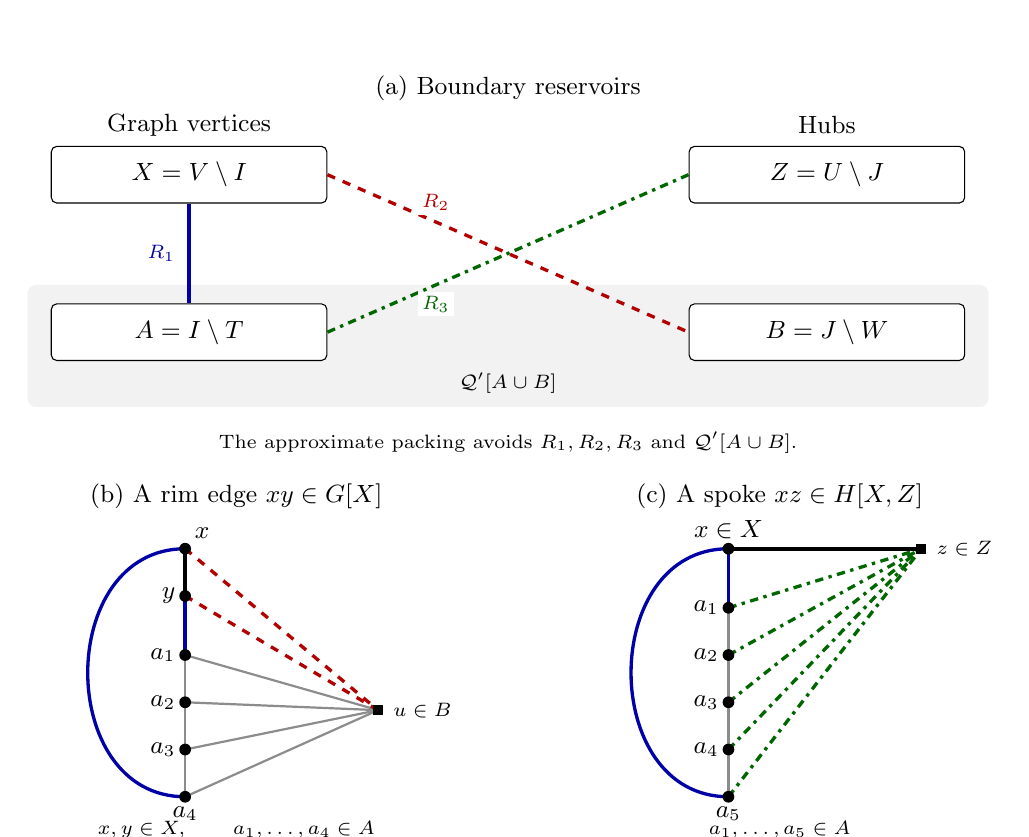
\begin{tikzpicture}[x=1cm,y=1cm,font=\small,
 rim/.style={circle,fill=black,inner sep=1.5pt},
 hub/.style={rectangle,fill=black,inner sep=1.8pt},
 rone/.style={blue!65!black,very thick},
 rtwo/.style={red!70!black,very thick,dashed},
 rthree/.style={green!40!black,very thick,dash dot},
 inner/.style={black!45,thick},
 prescribed/.style={black,line width=1.5pt},
 box/.style={draw,rounded corners=2pt,fill=white,minimum width=3.5cm,
             minimum height=.72cm,align=center},
 tag/.style={fill=white,inner sep=1.5pt,font=\scriptsize}]

\node at (6.65,4.45) {(a) Boundary reservoirs};
\node[font=\small] at (2.6,3.98) {Graph vertices};
\node[font=\small] at (10.7,3.98) {Hubs};
\fill[black!5,rounded corners=3pt] (.55,.4) rectangle (12.75,1.95);
\node[box] (X) at (2.6,3.35) {$X=V\setminus I$};
\node[box] (Z) at (10.7,3.35) {$Z=U\setminus J$};
\node[box] (A) at (2.6,1.35) {$A=I\setminus T$};
\node[box] (B) at (10.7,1.35) {$B=J\setminus W$};
\draw[rone] (X.south)--node[tag,left=3pt] {$R_1$} (A.north);
\draw[rtwo] (X.east)--node[tag,pos=.3,above=2pt] {$R_2$} (B.west);
\draw[rthree] (A.east)--node[tag,pos=.3,below=2pt] {$R_3$} (Z.west);
\node[font=\scriptsize] at (6.65,.7) {$\mathcal Q'[A\cup B]$};
\node[font=\scriptsize] at (6.65,-.05)
 {The approximate packing avoids $R_1,R_2,R_3$ and $\mathcal Q'[A\cup B]$.};

\begin{scope}[shift={(3.2,-2.85)}]
\node at (0,2.12) {(b) A rim edge $xy\in G[X]$};
\coordinate (x) at (-.65,1.45);
\coordinate (y) at (-.65,.85);
\coordinate (a1) at (-.65,.1);
\coordinate (a2) at (-.65,-.5);
\coordinate (a3) at (-.65,-1.1);
\coordinate (a4) at (-.65,-1.7);
\coordinate (u) at (1.8,-.6);
\draw[inner] (a1)--(a2)--(a3)--(a4);
\foreach \v in {a1,a2,a3,a4} {\draw[inner] (\v)--(u);}
\draw[rtwo] (x)--(u) (y)--(u);
\draw[rone] (y)--(a1);
\draw[rone] (a4) .. controls (-2.3,-1.7) and (-2.3,1.45) .. (x);
\draw[prescribed] (x)--(y);
\foreach \v in {x,y,a1,a2,a3,a4} {\node[rim] at (\v) {};}
\node[hub,label={[font=\scriptsize]right:$u\in B$}] at (u) {};
\node[above right] at (x) {$x$};\node[left] at (y) {$y$};
\node[left] at (a1) {$a_1$};\node[left] at (a2) {$a_2$};
\node[left] at (a3) {$a_3$};\node[below] at (a4) {$a_4$};
\node[font=\scriptsize] at (0,-2.12) {$x,y\in X,\qquad a_1,\ldots,a_4\in A$};
\end{scope}

\begin{scope}[shift={(10.1,-2.85)}]
\node at (0,2.12) {(c) A spoke $xz\in H[X,Z]$};
\coordinate (x) at (-.65,1.45);
\coordinate (a1) at (-.65,.7);
\coordinate (a2) at (-.65,.1);
\coordinate (a3) at (-.65,-.5);
\coordinate (a4) at (-.65,-1.1);
\coordinate (a5) at (-.65,-1.7);
\coordinate (z) at (1.8,1.45);
\draw[inner] (a1)--(a2)--(a3)--(a4)--(a5);
\foreach \v in {a1,a2,a3,a4,a5} {\draw[rthree] (\v)--(z);}
\draw[rone] (x)--(a1);
\draw[rone] (a5) .. controls (-2.3,-1.7) and (-2.3,1.45) .. (x);
\draw[prescribed] (x)--(z);
\foreach \v in {x,a1,a2,a3,a4,a5} {\node[rim] at (\v) {};}
\node[hub,label={[font=\scriptsize]right:$z\in Z$}] at (z) {};
\node[above] at (x) {$x\in X$};
\node[left] at (a1) {$a_1$};\node[left] at (a2) {$a_2$};
\node[left] at (a3) {$a_3$};\node[left] at (a4) {$a_4$};
\node[below] at (a5) {$a_5$};
\node[font=\scriptsize] at (0,-2.12) {$a_1,\ldots,a_5\in A$};
\end{scope}
\end{tikzpicture}
\caption{Boundary reservoirs and extensions of uncovered edges to ordinary
$6$-wheels. In (b) and (c), the prescribed edge is bold black;
gray edges lie in $\mathcal Q'[A\cup B]$. The other edges use the
reservoirs indicated in (a).}
\label{fig:cover-down:reservoirs-and-extensions}
\end{figure}


The rim-vertex choices below use the sets
\begin{equation}
\begin{aligned}
 A\cap N_{R_1}(S)\cap N_G(T)\cap N_H(u)
   &\quad(S\subseteq X,\ T\subseteq A,\ 1\le|S|+|T|\le2,\ u\in B),\\
 A\cap N_{R_1}(S)\cap N_G(T)\cap N_{R_3}(z)
   &\quad(S\subseteq X,\ |S|\le1,\ T\subseteq A,\
                    1\le|S|+|T|\le2,\ z\in Z).
\end{aligned}
\label{eq:covering:sampled-extensions:ordinary}
\end{equation}
Replacing $R_1$ by $G[X,A]$ and $R_3$ by $H[A,Z]$ gives
the corresponding sets before sampling.
Lemma~\ref{lem:completion:local-extensions} bounds each of their
sizes below by $2\beta_0a$, after a fixed decrease of $\beta_0$.
Conditional on $\mathcal Q'$, the expected sizes of the sampled sets
are at least $2\beta_0\tau^{|S|}a$ and
$2\beta_0\tau^{|S|+1}a$, respectively, hence at least
$2\beta_0\tau^2a$.
Each count depends on at most $2a$ independent boundary-edge
indicators, and changing one indicator changes it by at most one.
McDiarmid's bounded-differences inequality
(Theorem~\ref{thm:prelim:bounded-differences}) bounds its failure
probability by $\exp(-c_1\tau^4a)$ for a fixed $c_1>0$.
A union bound over the $O(N^3)$ displayed root tuples gives size
at least $\beta_0\tau^2a$ simultaneously, including for roots
chosen later. When $S=\varnothing$ in the first line, the set is
unchanged and has size at least $2\beta_0a$.
For $e=xy\in E(G[X])$, the endpoints are $(3d,\pi)$-separated.
The second bound in \eqref{eq:completion:ordinary-neighbourhoods} gives
\begin{equation*}
B_e:=B\cap N_H(x)\cap N_H(y),\qquad
 |B_e|=s^2|B|\pm \varepsilon_1|B|,
 \qquad |B_e|\ge s^2|B|/2.
\end{equation*}
Conditional on $\mathcal Q'$, the number of $u\in B_e$ with
$xu,yu\in E(R_2)$ has distribution $\operatorname{Bin}(|B_e|,\tau^2)$.
Chernoff's inequality (Lemma~\ref{lem:prelim:chernoff}) and a union
bound over the $O(N^2)$ edges give, with probability $1-o(1)$,
\begin{equation}
 |\{u\in B_e:xu,yu\in R_2\}|\ge s^2\tau^2|B|/4.
 \label{eq:covering:sampled-hubs:ordinary}
\end{equation}
Since $|B|\ge\omega_{\rm est}a/2$, this lower bound is at least
$\beta_0\tau^2a$ after a fixed reduction of $\beta_0$.

For $z\in Z$, let $A_z:=N_{R_3}(z;A)$ and $B_z:=\varnothing$;
for $x\in X$, let $A_x:=N_{R_1}(x;A)$ and $B_x:=N_{R_2}(x;B)$.
For $i\in X\dot\cup Z$, let $S_i:=A_i\cup B_i$.
These sets contain the vertices of the internal graphs for the factor
or endpoint assignment at $i$, excluding the outside root $i$.
They satisfy
\begin{equation}
 |S_i|\le C_{\rm cov}\tau a,\qquad |S_i\cap S_j|\le C_{\rm cov}\tau^2a\ (i\ne j),
 \qquad |\{i:z\in S_i\}|\le C_{\rm cov}\tau n.
 \label{eq:family:supports:ordinary}
\end{equation}
A vertex in $S_i\cap S_j$ for distinct outside roots $i,j$
requires two distinct boundary edges to be retained.
McDiarmid's bounded-differences inequality
(Theorem~\ref{thm:prelim:bounded-differences}) and a union bound give
\eqref{eq:family:supports:ordinary} with probability $1-o(1)$.

Lemma~\ref{lem:new:bernoulli-factor} will provide $C_r$-factors
at $z\in Z$ from the cycle family $\mathcal C_{\{z\}}$ on
$N_H(z;A)$. For $x\in X$ when $r=3$, it will provide triangle
factors from $\mathcal T_x$ on $N_H(x;B)\dot\cup N_G(x;A)$,
with one hub and two rim neighbors per triangle.
For $r\ge4$, the endpoint assignments at $x$ instead use
Theorem~\ref{thm:new:fresh-candidacy} followed by
Lemma~\ref{lem:pr:ordinary-endpoints}, as verified below.
For the two cycle families, the coefficient and absorber bounds follow from
Lemma~\ref{lem:completion:ordinary-local-factor} and
\eqref{eq:local:triangle-weighted-family}, respectively.
In each factor application, write $k_{\rm f}:=k_{\rm f}(i)$ for the value
of the parameter $k$. Then $c_{\rm fac}a\le k_{\rm f}\le a$.
For either family, let $r_{\rm f}$ be its cycle length and let $B_{\rm f}>1$
be its coefficient bound at scale $a$. At scale $k_{\rm f}$,
the coefficient bound is $B_{\rm f}c_{\rm fac}^{1-r_{\rm f}}$. An absorber lower bound
$a_{\rm f}a^{r_{\rm f}^2}$ gives $a_{\rm f}k_{\rm f}^{r_{\rm f}^2}$.
On a fixed vertex set there are at most $r!$ ordinary $r$-cycles
and at most one triangle of $\mathcal T_x$.
At these fixed bounds, the input tolerances of
Lemma~\ref{lem:new:bernoulli-factor} are
$\eta_{\rm fr}^{\rm ord}$ and $\eta_{\rm fr}^{\triangle}$, respectively.
For each $z\in Z$, the first conclusion of
Lemma~\ref{lem:completion:ordinary-local-factor}, with $J=\{z\}$,
supplies the cycle weight and absorber estimates on $N_H(z;A)$.
Writing $K_{\rm fac}$ for its error constant,
\eqref{eq:family:cover-profiles:ordinary} gives vertex-load error at most
$K_{\rm fac}(\delta_0+6d/a)+\varepsilon_1\le\eta_{\rm fr}^{\rm ord}$.
Thus the one-class case of Lemma~\ref{lem:new:bernoulli-factor} applies.
When $r=3$, we apply its two-class case to $\mathcal T_x$ on
$N_H(x;B)\dot\cup N_G(x;A)$, with multiplicities $(1,2)$.
The coefficient, vertex-sum and paired-absorber bounds in
\eqref{eq:local:triangle-weighted-family} hold before an exact ratio
between these class sizes is imposed.
Let $K_\triangle$ be the error constant in
Lemma~\ref{lem:completion:triangle-endpoint-factor}.
Since $|B|\ge\omega_{\rm est}a/2$ and $q=\varrho s$,
\begin{equation*}
 \frac{q\,d_P(x;A)}{2|B|s}=1\pm 2\delta_0/\omega_{\rm est},\qquad
 2\delta_0/\omega_{\rm est}+6K_\triangle d/a+\varepsilon_1
 \le\eta_{\rm fr}^{\triangle}.
\end{equation*}
The second inequality verifies the required vertex-load bound.
The balance bound and the positive spoke degree give
$|N_H(x;B)|\le|N_G(x;A)|\le4|N_H(x;B)|$,
as required in the two-class case of Lemma~\ref{lem:new:bernoulli-factor}.
Memberships in the two sampled classes use distinct edges of $R_2$
and $R_1$, and hence are independent. The exact ratio for the final
factor classes will follow from
\eqref{eq:completion:ordinary-boundary-divisibility}.
For $r\ge4$ and each $x\in X$, we apply
Theorem~\ref{thm:new:fresh-candidacy} to $H[N_G(x;A),N_H(x;B)]$.
Its ambient order parameter is $a=|A|$, its relative part-size
parameter is $c_{\rm end}$, and
$(p,b,\rho,p_*,\epsilon)=(s,6d,\tau,s_{\min}/2,\varepsilon_{\rm ep}/2)$.
The five estimates in \eqref{eq:local:ordinary-candidacy} follow
from the first bound in \eqref{eq:completion:ordinary-neighbourhoods}
with $(S,J_0)=(\{x\},\varnothing),(\{x\},\{u\})$ and the second
bound with $S=\{x\},\{x,v\},\{x,v,v'\}$.
For the last intersection, $v,v'\in N_G(x;A)$ are distinct
and satisfy $vv'\notin E(F_{\pi,3d})$.
Thus \ref{cover:ordinary:local} supplies the five inequalities in
\eqref{eq:local:ordinary-candidacy} with error $\varepsilon_1$,
before the boundary edges are sampled.
There are $O(N)$ factor or endpoint applications, each with
failure probability $O(N^{-10})$, since $k_{\rm f},a=\Theta(N)$.
Together with the concentration bounds for the $O(N^3)$ extension
tuples, common-hub counts and the sets $S_i$, this gives simultaneous
success probability $1-o(1)$.
The same concentration inequalities bound degree deviations by
$\eta n$ on the full domains and $\eta a$ on the inner restrictions,
simultaneously at all vertices and hubs.
For fixed $d,\tau,\eta$ and sufficiently large $N$, we fix an outcome
satisfying all these conclusions.

\paragraph{Step 2: Approximate wheel packing and covering the remaining edges on $X\cup Z$.}
The input for the approximate packing is $\mathcal Q^-:=\mathcal Q'-\mathcal Q'[A\cup B]-R_1-R_2-R_3$. Write
$G^-,H^-$ for its rim and spoke graphs.

Put $\gamma_0:=\tau^9=\gamma^{36}$, and let $\eta_{\rm pack}$ be
the balance tolerance supplied by
Lemma~\ref{lem:new:relative-ordinary-packing} with $\gamma=\gamma_0$
and the fixed parameters used for \ref{cover:ordinary:full}.
We take $\eta$ sufficiently small relative to
$\gamma_0,t_0,\eta_{\rm pack}$ and $1/C_{\rm cov}$.
For $v\in V_0$, let $b_0(v):=b_{\mathcal Q'}(v)$ and
$b_1(v):=b_{\mathcal Q'}^{A,B}(v)$.
The expected degree difference in $\mathcal Q^-$ is $-\tau b_1(v)$
for $v\in X$, since $b_0(v)=0$, and
$(1-\tau)(b_0(v)-b_1(v))$ for $v\in A$.
The bounds in \ref{cover:ordinary:balance} and the degree deviations
give $|b_{\mathcal Q^-}(v)|\le C_{\rm cov}\eta n$ for all $v\in V_0$.
The removed graph satisfies
$\Delta_*(\mathcal Q'-\mathcal Q^-)\le C_{\rm cov}(\epsilon+\tau)n\le t_0n$.
By \eqref{eq:packing:ordinary-deletion} and \ref{cover:ordinary:full},
\begin{equation*}
\begin{aligned}
 d_{H^-}(v)&\ge(2\omega_{\rm est}-t_0)n\ge\omega_{\rm est}n
       &&(v\in V_0),\\
 \widehat I_e(G^-,H^-)&\ge2\omega_{\rm est}-C_{\rm cov}t_0\ge\omega_{\rm est}
       &&(e\in E(G^-)),\\
 \widehat T_{v,u,u'}(G^-,H^-)&\ge2\omega_{\rm est}-C_{\rm cov}t_0\ge\omega_{\rm est}
       &&(v\in V_0,\ u\ne u'\in N_{H^-}(v)).
\end{aligned}
\end{equation*}
For $e\in E(G^-)\dot\cup E(H^-)$, the indicator of $e$ is one.
Inserting it into the potential-load sum does not change the sum,
so $\widehat L_e(G^-,H^-)$ equals the load of the restricted wheel
weighting at $e$.
Restricting $w_0$ to the remaining wheels therefore preserves its
coefficient bounds and gives edge-load error at most
$\varepsilon_0+C_{\rm cov}t_0\le2\varepsilon_0$.
Since $\min\{n,|U_0|\}\ge\omega_{\rm est}n/2$,
Lemma~\ref{lem:pr:cut-stability} gives cut coefficient at least
$2\omega_{\rm est}-2t_0/\omega_{\rm est}\ge\omega_{\rm est}$,
with the same cut threshold.
We apply Lemma~\ref{lem:new:relative-ordinary-packing} to $G^-,H^-$
on $(V_0,U_0)$, with $(P,\mathcal F)=(P_0,F_{\pi,3d}[V_0])$,
the restricted orientation and the restriction of $w_0$.
The parameters are the same $r,k,\alpha$, together with
\begin{equation*}
 \omega=\omega_{\rm est}/2,\qquad
 \beta=\delta_c=h_c=\omega_{\rm est},\qquad
 B_{\omega}=\omega_{\rm est}^{-1},\qquad \gamma=\gamma_0
\end{equation*}
in that lemma. The balance bound is $C_{\rm cov}\eta n\le\eta_{\rm pack}n$,
and the preceding degree, configuration, load and cut estimates
verify its other hypotheses.
Let $F_{\rm ap}$ be the union of the resulting wheels. Then
\begin{equation*}
 \Delta_*(\mathcal Q^--F_{\rm ap})\le\gamma_0n,\qquad
 E(F_{\rm ap})\cap
 \bigl(E(\mathcal Q'[A\cup B])\cup E(R_1)\cup E(R_2)\cup E(R_3)\bigr)
 =\varnothing.
\end{equation*}
In particular, every edge of
$(\mathcal Q'-F_{\rm ap})[X\cup Z]$ belongs to the graph
$\mathcal Q^--F_{\rm ap}$ of maximum degree at most $\gamma_0n$.

Put $\gamma_{\rm cov}:=\gamma_0^{1/3}=\gamma^{12}$.

We extend every edge of $(\mathcal Q'-F_{\rm ap})[X\cup Z]$
successively to an ordinary $r$-wheel, with disjoint edge sets
and all new vertices in $A\cup B$.
For a rim edge $xy$, the hub is chosen from the set in
\eqref{eq:covering:sampled-hubs:ordinary}. The remaining rim is an
$x$--$y$ path of length $r-1$ with internal vertices in $A$.
For a spoke $xz$, the hub is $z$ and all other rim vertices lie
in $A$, with their spokes in $R_3$.
All rim edges between $X$ and $A$ belong to $R_1$.
For $r=3$, a prescribed rim edge uses the first line of
\eqref{eq:covering:sampled-extensions:ordinary} with $S=\{x,y\}$.
For $r\ge4$, the first and last internal vertices use that line
with $(S,T)=(\{x\},\varnothing)$ and $(\{y\},\{w\})$,
respectively, where $w$ is the preceding rim vertex.
For a prescribed spoke, the corresponding choices use the second
line with $(S,T)=(\{x\},\varnothing)$ and $(\{x\},\{w\})$.
Intermediate choices use $S=\varnothing$, $T=\{w\}$ in the relevant line.

Let $f_{\rm cov}(v)$ and $g_{\rm cov}(u)$ count previous free choices
of $v\in A$ as a rim vertex and of $u\in B$ as a hub, respectively.
We choose $v\in A$ only when $f_{\rm cov}(v)<\sqrt{\gamma_0}n$,
and $u\in B$ only when $g_{\rm cov}(u)<\sqrt{\gamma_0}n$.
There are at most $C_{\rm cov}\gamma_0n^2$ free choices, so the usage limits
exclude at most $C_{\rm cov}\sqrt{\gamma_0}n$ candidates.
Together with the prescribed-edge degree bound $\gamma_0n$, these
limits bound the degree of each partial union by $C_{\rm cov}\sqrt{\gamma_0}n$.
Previously used edges therefore exclude another $C_{\rm cov}\sqrt{\gamma_0}n$
candidates. Excluding rim vertices at $\pi$-distance at most $3d$
from those already in the current wheel removes $O_r(d)$ more.
For sufficiently large $N$ in terms of $d$ and the fixed constants,
$C_{\rm cov}\sqrt{\gamma_0}n+O_r(d)\le\beta_0\tau^2a/2$, since
$a\ge\epsilon n/3$.
Thus every choice is possible, and the union has maximum degree
at most $C_{\rm cov}\sqrt{\gamma_0}n\le \gamma_{\rm cov}n$.
Each wheel contains only its prescribed edge inside $X\cup Z$.
Let $F_{\rm cov}$ be their union and
$\mathcal Q_{\rm rem}:=\mathcal Q'-F_{\rm ap}-F_{\rm cov}$. Then
\begin{equation*}
\mathcal Q_{\rm rem}[X\cup Z]=\varnothing,\qquad
 \Delta_*(F_{\rm cov})\le \gamma_{\rm cov}n.
\end{equation*}
Write $G_{\rm rem},H_{\rm rem}$ for the rim and spoke graphs.
Removing whole ordinary $r$-wheels preserves the degree equalities
at $X$ and the hub congruences at $Z$ in \ref{cover:ordinary:balance}, giving
\begin{equation}
 r\mid |N_{H_{\rm rem}}(z;A)|\quad(z\in Z),\qquad
 |N_{G_{\rm rem}}(x;A)|=2|N_{H_{\rm rem}}(x;B)|\quad(x\in X).
 \label{eq:completion:ordinary-boundary-divisibility}
\end{equation}
Indeed, no remaining spoke joins $X$ to $Z$ and no remaining
rim edge has both endpoints in $X$.

\paragraph{Step 3: Selecting factors and endpoint assignments for the boundary.}
The boundary edges now lie in
$G_{\rm rem}[X,A]$, $H_{\rm rem}[X,B]$ and $H_{\rm rem}[A,Z]$.
The exact identities
\eqref{eq:completion:ordinary-boundary-divisibility} give the
divisibility and class sizes required for the local factors.
For $x\in X$, let $A_x':=N_{G_{\rm rem}}(x;A)$ and
$B_x':=N_{H_{\rm rem}}(x;B)$; for $z\in Z$, let
$A_z':=N_{H_{\rm rem}}(z;A)$ and $B_z':=\varnothing$.
Let $S_i':=A_i'\cup B_i'$.
Every edge of $G_{\rm rem}[X,A]-R_1$, $H_{\rm rem}[X,B]-R_2$
or $H_{\rm rem}[A,Z]-R_3$ belongs to $\mathcal Q^--F_{\rm ap}$.
Conversely, every edge of $R_1\cup R_2\cup R_3$ absent from
$\mathcal Q_{\rm rem}$ belongs to $F_{\rm cov}$.
Hence, with $L_{\rm ch}:=C_{\rm cov}(\gamma_0+\gamma_{\rm cov})n$, we have
\begin{equation*}
|S_i'\triangle S_i|\le L_{\rm ch} \quad (i\in X\dot\cup Z),\qquad |\{i:z\in S_i'\triangle S_i\}|\le L_{\rm ch} \quad (z\in A\dot\cup B).
\end{equation*}
By the hierarchy and $a\ge\epsilon n/3$,
we have
$L_{\rm ch}\le\min\{\zeta\tau a,\tau^2a\}$.
In particular,
\begin{equation*}
 |S_i'\cap S_j'|\le |S_i\cap S_j|+2L_{\rm ch}\quad(i\ne j),\qquad
 |\{i:z\in S_i'\}|\le|\{i:z\in S_i\}|+L_{\rm ch}.
\end{equation*}
Together with \eqref{eq:family:supports:ordinary}, these give
$|S_i'|\le C_S\tau a$, $|S_i'\cap S_j'|\le C_S\tau^2a$ for $i\ne j$,
and $|\{i:z\in S_i'\}|\le C_S\tau n$, with $C_S$ including the losses.
Since $A,B$ are disjoint,
$|A_i'\triangle A_i|+|B_i'\triangle B_i|=|S_i'\triangle S_i|
\le\zeta\tau a$, as required by the sampling results.
Also $\mathcal Q_{\rm rem}\subseteq\mathcal Q'$ ensures that the
new classes lie in the original neighbor sets in $G,H$.

For $z\in Z$, let $\mathcal F_z$ consist of the $C_r$-factors in
$G_{\rm rem}[A_z']$ whose cycles have $F_{\pi,3d}$-independent vertex sets.
For $x\in X$ and $r=3$, let $\mathcal F_x$ consist of the factors
on $A_x'\dot\cup B_x'$ from the family $\mathcal T_x$ restricted
to $G_{\rm rem},H_{\rm rem}$.
For $x\in X$ and $r\ge4$, let $\mathcal F_x$ consist of the graphs
with edge set $\{v_uu,w_uu:u\in B_x'\}$ arising from partitions
$A_x'=\dot\bigcup_{u\in B_x'}\{v_u,w_u\}$ with
$v_uu,w_uu\in E(H_{\rm rem})$ and
$\operatorname{dist}_\pi(v_u,w_u)>3d$.
These candidates contain only internal edges; the edges incident
with the outside root are added after selection.
Each candidate has maximum degree at most two.

Since $F_{\rm ap}[A\cup B]=\varnothing$, we have
$\mathcal Q_{\rm rem}[A\cup B]
=\mathcal Q'[A\cup B]-F_{\rm cov}[A\cup B]$.
Let $J_{\rm int}$ be the simple graph on $A\dot\cup B$ with edge set
$E(G[A])\dot\cup E(H[A,B])$. Every member of $\mathcal F_i$ is a
subgraph of $J_{\rm int}[S_i']$.
We apply Lemma~\ref{lem:new:bounded-degree-selection} in $J_{\rm int}$,
with $n_S:=a+|B|$, $D_0=4$, $p_{\rm sel}:=C_{\rm sel}\tau/\epsilon<1$
and the sets $S_i'$.
Since $a\ge\epsilon n/3$ and $a\le n_S=a+|B|\le2a$,
we have $C_S\tau n\le p_{\rm sel}n_S$ and
$C_S\tau^2a\le p_{\rm sel}^2n_S$.
The bounds above on the number of sets $S_i'$ containing each vertex
and on their pairwise intersections therefore verify the membership
and intersection hypotheses.
To verify the remaining hypothesis of
Lemma~\ref{lem:new:bounded-degree-selection}, we fix $i\in X\dot\cup Z$
and a graph $J_i\subseteq J_{\rm int}[S_i']$ with
$\Delta(J_i)\le4p_{\rm sel}^{3/2}n_S$.
We construct $t_{\rm sel}:=\lceil4p_{\rm sel}^{3/2}n_S\rceil$
edge-disjoint members of the fixed family $\mathcal F_i$ avoiding $J_i$.
At each choice, let $J_{\rm forb}$ be the union of $J_i$, the
previously chosen candidates for this $i$, and the edges of
$F_{\rm cov}$ inside $A\cup B$.
Its maximum degree is at most
$4p_{\rm sel}^{3/2}n_S+4t_{\rm sel}+\gamma_{\rm cov}n
\le C_4p_{\rm sel}^{3/2}a+4+\gamma_{\rm cov}n<\zeta\tau a$. Here, $C_4=40$ suffices
since $n_S\le2a$.
The last inequality follows from
$\tau=\gamma^4$, $\gamma_{\rm cov}=\gamma^{12}$ and the hierarchy, for sufficiently
large $N$. For the sampling outcome fixed in the first construction,
Lemma~\ref{lem:new:bernoulli-factor}, with $\rho=\tau$, applies at
$z\in Z$ with $(U,k,c)=(N_H(z;A),|N_H(z;A)|,r)$ and $U''=A_z'$.
At $x\in X$ when $r=3$, its two-class case has
$(A,B_1,k,c)=(N_H(x;B),N_G(x;A),|N_H(x;B)|,3)$ and
$U''=B_x'\dot\cup A_x'$.
The bounds $|S_i'\triangle S_i|\le\zeta\tau a$ established above
give the required set changes, and the required divisibility and
exact class ratio follow from
\eqref{eq:completion:ordinary-boundary-divisibility}.
The lemma supplies a factor avoiding $J_{\rm forb}$.

For $r\ge4$, let $m_x:=|B_x'|$, so $|A_x'|=2m_x$.
Theorem~\ref{thm:new:fresh-candidacy} supplies degree and cut bounds
for $H_{\rm rem}[A_x',B_x']-J_{\rm forb}[A_x',B_x']$.
Here, its density lower bound $p_*=s_{\min}/2$ gives degree and cut
coefficient $s_{\min}/4$, and its relative cut threshold
$\varepsilon_{\rm ep}/2$ includes all cuts with both parts of size
at least $\varepsilon_{\rm ep}m_x$.
Thus Lemma~\ref{lem:pr:ordinary-endpoints} applies to this graph
with $\lambda=s_{\min}/4$, $m=m_x$, $B_0=F_{\pi,3d}[A_x']$ and
$b_0=6d$, giving the next endpoint assignment.
Lemma~\ref{lem:new:bounded-degree-selection} therefore selects one
graph $F_i\in\mathcal F_i$ for each $i\in X\dot\cup Z$, with
pairwise disjoint edge sets and
$\Delta(\bigcup_iF_i)\le4p_{\rm sel}n_S\le C_{\rm cov}\tau n$.
For $z\in Z$, each cycle of $F_z$, together with its spokes to $z$,
forms an ordinary $r$-wheel. These wheels cover all remaining spokes at $z$. For a triangle $\{v,w,u\}$ in $F_x$,
adjoining $xv,xw,xu$ gives an ordinary $3$-wheel.

\paragraph{Step 4: Completing the assigned paths inside $A$.}
For $r=3$, the preceding factors already cover all boundary
edges. For $r\ge4$, each assignment at $x\in X$ consists of rim
neighbors $v,w\in A$ and a hub $u\in B$, with spokes $vu,wu$.
All endpoint spokes in the selected graphs $F_x$ are reserved
before any internal path vertex is chosen.
We join $v$ to $w$ by a path of length $r-2$ in $A\cap N_H(u)$.
Together with $xv,xw,xu$ and the spokes of its vertices, this gives
an ordinary $r$-wheel with hub $u$.

These paths use $G[A]$ and $H[A,B]$, which were not sampled in
the first construction and were not used by $F_{\rm ap}$.
For $r=4$, the internal vertex lies in
$A\cap N_G(v)\cap N_G(w)\cap N_H(u)$.
For $r\ge5$, successive vertices need one rim adjacency, except
for the last, which is adjacent to the preceding vertex and $w$.
Each must also be adjacent to $u$ in $H$.
Lemma~\ref{lem:completion:local-extensions} gives at least $\beta_0a$
choices in each case, after a fixed decrease of $\beta_0$.
The bound on $\Delta(\bigcup_iF_i)$ implies that each endpoint and
assigned hub occurs in at most $C_{\rm cov}\tau n$ pairs.
Let $f_{\rm path}(v)$ count previous choices of $v\in A$ as an
internal path vertex. We choose $v$ only while $f_{\rm path}(v)<\sqrt\tau n$.
There are $O_r(\tau n^2)$ such choices in total, so at most
$C_{\rm cov}\sqrt\tau n$ vertices have reached this limit.
The selected graphs $F_i$, $F_{\rm cov}$ and the paths already
constructed have internal degree at most $C_{\rm cov}\sqrt\tau n$.
We avoid all previously used edges and all reserved endpoint spokes
other than the two reserved for the current pair.
These exclusions remove at most $C_{\rm cov}\sqrt\tau n$ candidates,
and separation excludes $O_r(d)$ more.
The bound $a\ge\epsilon n/3$ gives
$C_{\rm cov}\sqrt\tau n+O_r(d)\le\beta_0a/2$ for sufficiently large $N$
in terms of $d$ and the fixed constants, so all paths can be completed.

Let $F_{\partial}$ be the union of the wheels obtained from the
boundary factors and the completed paths. Every edge of
$\mathcal Q_{\rm rem}$ incident with $X\cup Z$ lies in $F_{\partial}$.
Thus the extended graph
$\mathcal Q_{\rm next}:=\mathcal Q_{\rm rem}-F_{\partial}$
has all its edges on $(A,B)$, and
\begin{equation*}
 \mathcal Q_{\rm next}\subseteq\mathcal Q'[A\cup B],\qquad
 F_U:=F_{\rm ap}\cup F_{\rm cov}\cup F_{\partial}.
\end{equation*}
The graphs $F_{\rm ap},F_{\rm cov},F_{\partial}$ have
pairwise disjoint edge sets.
Since $F_{\rm ap}$ uses no edge inside $A\cup B$, we have
$\Delta_*(F_U[A\cup B])\le \gamma_{\rm cov}n+C_{\rm cov}\sqrt\tau n\le\nu n\le\nu N$.
This proves \eqref{eq:completion:active-output:ordinary}.
\end{proof}

\begin{localclaim}[The next divisible remainder]\label{clm:protected:restore:ordinary}
The remainder $\mathcal R':=\mathcal R-F_E-F_D-F_U$ is $r$-wheel-divisible,
is an extended subgraph of $\mathcal R[I\cup J]$, and satisfies
\eqref{eq:family:protected-output:ordinary}. In fact,
\begin{equation}
 E(\mathcal R[I\cup J]-\mathcal R')
 =E_{\rm del}\dot\cup E(F_U[I'\cup J']).
 \label{eq:completion:one-level-remainder:ordinary}
\end{equation}
\end{localclaim}

Figure~\ref{fig:cover-down:inner-edge-use} shows the locations of the
two edge sets in this identity.
\begin{figure}[htbp]
\centering
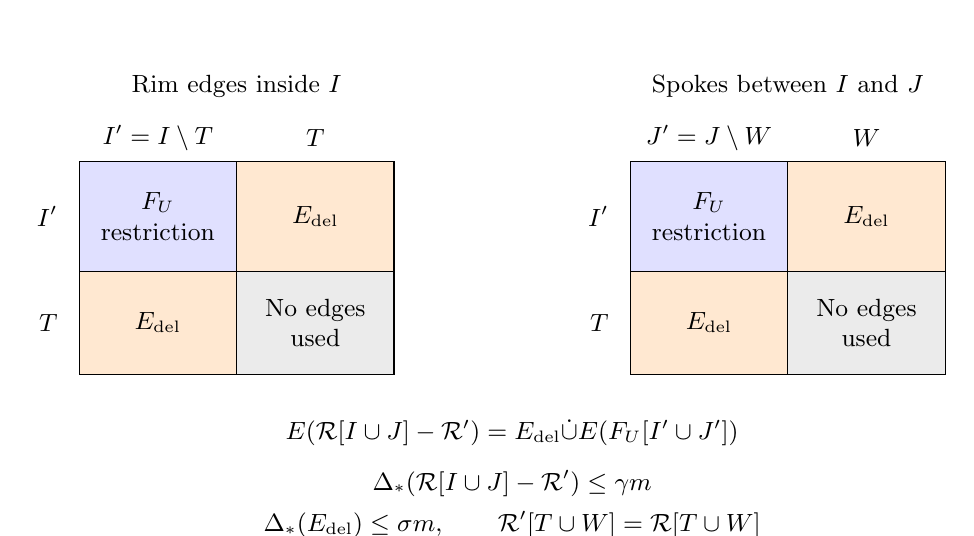
\begin{tikzpicture}[x=1cm,y=1cm,font=\small,>=stealth,
 dot/.style={circle,fill=black,inner sep=1.5pt},
 first/.style={blue!65!black,thick},
 second/.style={red!70!black,thick,dashed},
 shared/.style={green!35!black,very thick},
 spoke/.style={black!45,thin},
 tag/.style={fill=white,inner sep=1pt,font=\scriptsize}]

\node at (2,3.65) {Rim edges inside $I$};
\node at (9,3.65) {Spokes between $I$ and $J$};
\node at (1,3) {$I'=I\setminus T$}; \node at (3,3) {$T$};
\node[anchor=east] at (-.15,2) {$I'$}; \node[anchor=east] at (-.15,.65) {$T$};
\fill[blue!12] (0,1.3) rectangle (2,2.7);
\fill[orange!18] (2,1.3) rectangle (4,2.7);
\fill[orange!18] (0,0) rectangle (2,1.3);
\fill[black!8] (2,0) rectangle (4,1.3);
\draw (0,0) rectangle (4,2.7);\draw (2,0)--(2,2.7);\draw (0,1.3)--(4,1.3);
\node[align=center] at (1,2) {$F_U$\\restriction};
\node at (3,2) {$E_{\rm del}$};\node at (1,.65) {$E_{\rm del}$};
\node[align=center] at (3,.65) {No edges\\used};
\node at (8,3) {$J'=J\setminus W$}; \node at (10,3) {$W$};
\node[anchor=east] at (6.85,2) {$I'$}; \node[anchor=east] at (6.85,.65) {$T$};
\fill[blue!12] (7,1.3) rectangle (9,2.7);
\fill[orange!18] (9,1.3) rectangle (11,2.7);
\fill[orange!18] (7,0) rectangle (9,1.3);
\fill[black!8] (9,0) rectangle (11,1.3);
\draw (7,0) rectangle (11,2.7);\draw (9,0)--(9,2.7);\draw (7,1.3)--(11,1.3);
\node[align=center] at (8,2) {$F_U$\\restriction};
\node at (10,2) {$E_{\rm del}$};\node at (8,.65) {$E_{\rm del}$};
\node[align=center] at (10,.65) {No edges\\used};
\node[align=center] at (5.5,-.75)
 {$E(\mathcal R[I\cup J]-\mathcal R')=E_{\rm del}\dot\cup E(F_U[I'\cup J'])$};
\node[align=center] at (5.5,-1.65)
 {$\Delta_*(\mathcal R[I\cup J]-\mathcal R')\le\gamma m$\\[4pt]
  $\Delta_*(E_{\rm del})\le\sigma m,\qquad
    \mathcal R'[T\cup W]=\mathcal R[T\cup W]$};

\end{tikzpicture}
\caption{Edges used inside $(I,J)$ in a cover-down step.
The cells indicate the possible locations of edges in $E_{\rm del}$
and $F_U[I'\cup J']$. The used edges incident with $T\cup W$ are
precisely those in $E_{\rm del}$, and the induced graph on $(T,W)$
is unchanged. In the marked case, rim endpoints are auxiliary vertices.}
\label{fig:cover-down:inner-edge-use}
\end{figure}

\begin{proof}
The packings avoid $\mathcal K$, so $\mathcal K\subseteq\mathcal R'$.
Since $\mathcal R$ is $r$-wheel-divisible and each removed wheel
is an ordinary $r$-wheel, $\mathcal R'$ is $r$-wheel-divisible.
Claim~\ref{clm:protected:deep:ordinary} covers every edge of
$\mathcal Q_0$ incident with $T\cup W$, while the retained graph
$\mathcal K$ lies in $\mathcal R[I\cup J]$.
Claim~\ref{clm:protected:active:ordinary} covers all other remaining
edges outside $I'\cup J'$. Hence $\mathcal R'\subseteq\mathcal R[I\cup J]$.
Within $(I,J)$, $F_E$ uses exactly $E_{\rm del}$, $F_D$ uses no edge,
and $F_U$ uses exactly its restriction to $(I',J')$.
This proves \eqref{eq:completion:one-level-remainder:ordinary}.
The degree of the graph removed inside $I\cup J$ satisfies
$\Delta_*(\mathcal R[I\cup J]-\mathcal R')
\le C_{\rm cov}\xi m+\nu N\le(C_{\rm cov}\xi+2\nu/\epsilon)m\le\gamma m/50<\gamma m$,
since $m\ge\epsilon N/2$, $C_{\rm cov}\xi\le\gamma/100$ and $\nu=\gamma\epsilon/200$.
Among its edges, those incident with $T\cup W$ are exactly $E_{\rm del}$,
with $\Delta_*(E_{\rm del})\le C_{\rm cov}\xi m\le\sigma m$.
Finally, $D[T\cup W]=\varnothing$ and
$F_U\subseteq\mathcal Q'[V'\cup U']$ give
$\mathcal R'[T\cup W]=\mathcal R[T\cup W]$.
When $T=W=\varnothing$, we have $I'=I$ and $J'=J$, and
$\mathcal K,E_{\rm del},F_E,F_D$ are empty. Thus
$\mathcal R'=\mathcal R-F_U$, where $F_U$ is the union of the wheels
supplied by Claim~\ref{clm:protected:active:ordinary}.
\end{proof}
The union of the three packings proves the lemma.

\end{proof}

\section{Marked cover-down}
Given a physically injective, marked $c$-wheel-divisible completion
host $\mathcal R$ satisfying the estimates below,
Lemma~\ref{lem:completion:marked-cover-down} produces a packing of
marked $c$-wheels that leaves a marked $c$-wheel-divisible remainder
on $(I,J)$. The used edges inside $(I,J)$ have $\Delta_*$ at most
$\gamma|I|$. Their intersection with $\operatorname{star}(T,W)$ has
$\Delta_*$ at most $\sigma|I|$, and no edge of
$\mathcal R[T\cup W]$ is used. In $\operatorname{star}(T,W)$,
incidence is determined by the auxiliary endpoints of each typed
arc or spoke.
The proof of Proposition~\ref{prop:completion:marked-construction}
iterates this step and absorbs the terminal remainder.

\subsection{Marked local cycle estimates}
In the local estimates, $A,B$ are summation domains and $X,Y$
contain the possible vertex and hub roots. These estimates are used
to construct cycle factors and path extensions with the prescribed
types. We use $0<\omega_{\rm est}\le1/8$ as a common lower bound
and its reciprocal as a coefficient upper bound.

\begin{definition}[Marked local cycle estimates]\label{gls:marked-local-cycle-estimates}
\label{def:completion:marked-local-estimates}
Let $V,U$ be disjoint, let $P$ be a graph on $V$, let $\pi$ be a permutation of $V$, let $c\ge8$ be an even integer,
and let $d\ge2$ be an integer.
Let $\mathcal Q=(V,U,R^0,R^K,H^0,H^K)$ be a marked completion host
on $(P,V,U,\pi)$ with separation parameter $d$.
Let
$A\subseteq X\subseteq V$, $B\subseteq Y\subseteq U$,
$a=|A|>0$, $p,k,s,t>0$, $0<\omega_{\rm est}\le1/8$, $\mu>0$ and $\eta\ge0$.
Assume $\pi(A)=A$.

Recall from \eqref{eq:endpoints:potential-rims} that
$\overline R^0$ consists of the arcs $x\to y$ on $V$ with
$\operatorname{dist}_\pi(x,y)>3d$ and $xy\in E(P)$.
For $\overline R^K$, the conditions are
$\operatorname{dist}_\pi(x,y)>3d$ and $x\pi(y)\in E(P)$.
Let $p_0:=p$, $p_K:=k$, $s_0:=s$ and $s_K:=t$.

The family $\mathcal C_P^A$ in
\eqref{eq:completion:parent-marked-cycles} consists of typed directed
$c$-cycles on $A$ with exactly one type-$K$ arc, a
$(3d,\pi)$-separated vertex set and distinct physical edges in $P$.
Membership does not require the arcs or spokes to be present in
$\mathcal Q$. Let $\omega_A$ be a fixed positive weighting on
$\mathcal C_P^A$ satisfying
\begin{equation*}
 \omega_{\rm est}a^{1-c}\le\omega_A(C)\le\omega_{\rm est}^{-1}a^{1-c}
 \quad(C\in\mathcal C_P^A).
\end{equation*}

The host $\mathcal Q$ has \emph{marked local cycle estimates}
relative to $\omega_A$,
with error $\eta$ and count multiplier $\mu$ on $(A,B;X,Y)$, if
all the following estimates hold.

\emph{Neighborhood estimates.} For every $j\in\{0,K\}$ and $J_0\subseteq Y$ with $|J_0|\le3$,
\begin{equation}
 |A\cap N_{H^j}(J_0)|=s_j^{|J_0|}a\pm \eta a.
 \label{eq:completion:marked-spoke-intersections}
\end{equation}
The rim-neighborhood estimates are
\begin{equation}
\begin{aligned}
 |A\cap N_{R^\tau}^{e}(x)\cap N_{H^j}(J_0)|&=p_\tau s_j^{|J_0|}|A\cap N_{\overline R^\tau}^{e}(x)|\pm \eta a,\\
 |A\cap N_{R^0}^{+}(x)\cap N_{R^0}^{-}(y)\cap N_{H^0}(u)|&=p^2s|A\cap N_{\overline R^0}^{+}(x) \cap N_{\overline R^0}^{-}(y)|\pm \eta a,\\
 |A\cap N_{R^0}^{+}(x)\cap N_{R^K}^{-}(y)\cap N_{H^0}(u)|&=pks|A\cap N_{\overline R^0}^{+}(x) \cap N_{\overline R^K}^{-}(y)|\pm \eta a.
\end{aligned}
\label{eq:completion:marked-row-patterns}
\end{equation}
In the first line, $x\in X$, $J_0\subseteq Y$ with $|J_0|\le1$, and
$(\tau,e,j)\in\{(0,+,0),(0,-,0),(K,-,0),(K,+,K)\}$.
In the last two lines, $x,y\in X$ and $u\in Y$.
The second has $x\ne y$, and the third has $x\ne\pi(y)$.
These restrictions make the two required physical edges distinct.

For all disjoint $S_0,S_K\subseteq X$ with $(3d,\pi)$-separated union
and $|S_0|+|S_K|\le3$,
\begin{equation}
 |B\cap N_{H^0}(S_0)\cap N_{H^K}(S_K)|=s^{|S_0|}t^{|S_K|}|B|\pm \eta|B|.
 \label{eq:completion:marked-hub-intersections}
\end{equation}

\emph{Loads and cycle counts.} For each $u\in Y$, the potential load
$\widehat Z^A_{v,u,j}$ is defined by \eqref{eq:loads:marked-local-potential}
with $\omega_{A,u}=\omega_A$ and omits only the indicator of the root spoke $(v,u,j)$.
Recall that
$\mathcal C^A(u)=\{C\in\mathcal C_P^A:(C,u)\in
\mathcal W_c^K(\mathcal Q;3d,\pi)\}$.
For $b=3d$, the family $\mathcal F_j^A(v,v';u)$ consists of the
ordered tuples $\mathbf z\in\mathcal F_j(v,v';u)\cap A^{c-1}$,
where $\mathcal F_j(v,v';u)$ is defined by
\eqref{eq:marked:one-hub-paths} in $\mathcal Q$.
A tuple $\mathbf z=(z_1,\ldots,z_{c-1})$ specifies the two rooted
cycles $C_j(v,\mathbf z)$ and $C_j(v',\mathbf z)$, which share the
auxiliary directed path $z_1\cdots z_{c-1}$. The prescribed spokes at the free labels
must be present at $u$, whereas neither root spoke $(v,u,j)$ nor
$(v',u,j)$ is required.

These loads and families satisfy
\begin{equation}
\begin{aligned}
 \widehat Z^A_{v,u,j}&=1\pm \eta
       &&(v\in A,\ u\in Y,\ j\in\{0,K\}),\\
 |\mathcal C^A(u)|&\ge\mu\omega_{\rm est}a^c &&(u\in Y),\\
 |\mathcal F_j^A(v,v';u)|&\ge\mu\omega_{\rm est}a^{c-1}
       &&(v\ne v'\in A,\ u\in Y,\ j\in\{0,K\}).
\end{aligned}
\label{eq:protected:marked-local-loads}
\end{equation}
The multiplier $\mu$ is one when omitted.

\end{definition}

\subsection{Marked cover-down}
Let $V,U$ be disjoint finite sets, let $P$ be a simple graph on $V$,
and let $\pi$ be a permutation of $V$. Let
$T\subseteq I\subseteq V$ and $W\subseteq J\subseteq U$.
We write
\begin{equation*}
\begin{gathered}
N:=|V|,\quad M:=|U|,\quad m:=|I|,\qquad
 V':=V\setminus T,\quad U':=U\setminus W,\\
I':=I\setminus T,\quad J':=J\setminus W,\quad n':=|V'|,\quad m':=|I'|.
\end{gathered}
\end{equation*}

\begin{definition}[Marked completion estimates]\label{gls:marked-completion-estimates}
\label{def:completion:marked-estimates}
Let $c\ge8$ be an even integer, let $d\ge2$ be an integer, and let
$0<\varrho\le1$, $0<s\le1/100$, $\alpha,\epsilon>0$ and $0<\omega_{\rm est}\le1/8$.
Let $p:=\varrho s/2$, $\alpha_c:=\alpha/4$, $\delta_c:=\min\{\alpha/64,p/128\}$ and $h_c:=\alpha p/64$.

Let $\mathcal R=(R^0_{\mathcal R},R^K_{\mathcal R},H^0_{\mathcal R},H^K_{\mathcal R})$
be a marked completion host on $(P,V,U,\pi)$.
The cycle functions $\omega_A$ and the wheel weighting
$w_0$ specified below are fixed on their respective domains when
$\mathcal R$ varies.

For $\delta_{\rm deg},\eta_{\rm bal},\delta_{\rm bal},\varepsilon_*>0$
and $\mu>0$, we say that $\mathcal R$ has
\emph{marked completion estimates} with parameters
$(\delta_{\rm deg},\eta_{\rm bal},\delta_{\rm bal},\varepsilon_*;\mu)$
if the following conditions hold.

Here $\delta_{\rm deg}$ controls the degree errors in $P$, and
$\varepsilon_*$ controls the neighborhood, rim-degree and load errors.
The parameter $\mu$ scales the count lower bounds in
\ref{item:completion:marked:local}--\ref{item:completion:marked:potential},
the two-step neighborhood bound in \ref{item:completion:marked:potential},
and the cut coefficients in \ref{item:completion:marked:cuts}.
It is understood to be $1$ when omitted.

\begin{enumerate}[label=\textup{(M\arabic*)},itemsep=3pt]
\item\label{item:completion:marked:geometry}
\emph{Set sizes, permutation invariance and degrees in $P$.}
The size and invariance conditions are
\begin{equation}
\begin{gathered}
 \omega_{\rm est} N\le M\le N,\quad \epsilon N/2\le m\le\epsilon N,\quad
 \omega_{\rm est} m\le|J|\le m,\\
 |T|+|W|\le2\epsilon m,\qquad \pi(I)=I,\qquad\pi(T)=T.
\end{gathered}
 \label{eq:protected:geometry:marked}
\end{equation}
The degrees in $P$ satisfy
\begin{equation}
\begin{gathered}
 d_P(v)=2M/\varrho\pm \delta_{\rm deg} N/4,\quad
 d_P(v;I)=2|J|/\varrho\pm \delta_{\rm deg} m/4,\quad
 d_P(v;T)=2|W|/\varrho\pm \delta_{\rm deg} m/4,\\
 d_P(v)\ge(1/2+10\alpha)N,\quad
 d_P(v;I)\ge(1/2+10\alpha)m\qquad(v\in V).
\end{gathered}
\label{eq:family:protected-profiles:marked}
\end{equation}

\item
\emph{Restricted balance.} For $A\subseteq V$, $B\subseteq U$ and
all $v\in V$, $u\in U$, recall the four differences
\begin{equation*}
\begin{aligned}
 a_{\mathcal R}^{+,A,B}(v)&=d_{R_{\mathcal R}}^+(v;A)-d_{H_{\mathcal R}}(v;B),&
 a_{\mathcal R}^{-,A,B}(v)&=d_{R_{\mathcal R}}^-(v;A)-d_{H_{\mathcal R}}(v;B),\\
 a_{\mathcal R}^{K,A,B}(v)&=d_{R_{\mathcal R}^K}^-(v;A)-d_{H_{\mathcal R}^K}(v;B),&
 a_{\mathcal R}^{U,A}(u)&=d_{H_{\mathcal R}^0}(u;A)-(c-1)d_{H_{\mathcal R}^K}(u;A).
\end{aligned}
\end{equation*}
Here $R_{\mathcal R}:=R_{\mathcal R}^0\dot\cup R_{\mathcal R}^K$ and
$H_{\mathcal R}:=H_{\mathcal R}^0\dot\cup H_{\mathcal R}^K$.
We\phantomsection\label{gls:restricted-balance-differences:norm} write
\begin{equation*}
 \|\mathbf a_{\mathcal R}^{A,B}\|_{X,Y}
 :=\max\{\max_{v\in X,\,j\in\{+,-,K\}}|a_{\mathcal R}^{j,A,B}(v)|,
          \max_{u\in Y}|a_{\mathcal R}^{U,A}(u)|\}.
\end{equation*}
The differences over $(I,J)$ and $(T,W)$ satisfy the following
bounds, both normalized by $m=|I|$:
\begin{equation}
\begin{aligned}
 \max\{\|\mathbf a_{\mathcal R}^{I,J}\|_{V,U},\|\mathbf a_{\mathcal R}^{T,W}\|_{V,U}\}
 &\le\eta_{\rm bal}m,\\
 \max\{\|\mathbf a_{\mathcal R}^{I,J}\|_{I,J},\|\mathbf a_{\mathcal R}^{T,W}\|_{I,J}\}
 &\le\delta_{\rm bal}m.
\end{aligned}
\label{eq:protected:marked-reference-errors}
\end{equation}

\item\label{item:completion:marked:local}
\emph{Local cycle estimates.} The graph $\mathcal R$ satisfies the marked
local cycle estimates of Definition~\ref{def:completion:marked-local-estimates}
on the following domains:
\begin{equation*}
\begin{array}{c|c}
 \text{summation domains }(A,B)&\text{root sets }(X,Y)\\\hline
 (V,U)&(V,U)\\
 (I',J')&(V',U').
\end{array}
\end{equation*}
In both cases, we use $t:=s/(c-1)$, $k:=\varrho t/2$ and
$(p_0,p_K,s_0,s_K)=(p,k,s,t)$, with error $\varepsilon_*$,
coefficient bounds $\omega_{\rm est},\omega_{\rm est}^{-1}$ and
count multiplier $\mu$.

\item\label{item:completion:marked:potential}
\emph{Wheel weights and packing estimates.} Let $D':=2|U'|/\varrho$.
Let $w_0(W(C,u))>0$ be fixed coefficients indexed by $u\in U'$
and $C\in\mathcal C_P^{V'}$, where $\mathcal C_P^{V'}$ is the cycle family
in \eqref{eq:completion:parent-marked-cycles} with $A=V'$.
They satisfy
\begin{equation}
\begin{aligned}
 w_0(W(C,u))&=w_0(W(C,u'))
       &&(C\in\mathcal C_P^{V'},\ u,u'\in U'),\\
 \omega_{\rm est}(n')^{1-c}\le w_0(W(C,u))
       &\le\omega_{\rm est}^{-1}(n')^{1-c}
       &&(C\in\mathcal C_P^{V'},\ u\in U').
\end{aligned}
 \label{eq:protected:marked-weight-data}
\end{equation}

The following bounds are evaluated in $\mathcal R[V'\cup U']$.
\begin{subequations}\label{eq:protected:marked-full-data}
For $v\in V'$ and distinct $x,y\in V'$,
\begin{equation}
\begin{gathered}
 d^\pm_{R^0_{\mathcal R}}(v;V')=pD'\pm \varepsilon_*n',\qquad
 d^\pm_{R^K_{\mathcal R}}(v;V')=pD'/(c-1)\pm \varepsilon_*n',\\
 |N^+_{R^0_{\mathcal R}}(x;V')\cap N^-_{R^0_{\mathcal R}}(y;V')|
 \ge8\mu\alpha_cp^2n'.
 \label{eq:protected:marked-rim-data}
\end{gathered}
\end{equation}

The quantity $\widehat H_C$ counts the hubs in $U'$ joined to every
vertex of $C$ by a spoke of its prescribed type, regardless of
whether the rim arcs of $C$ are present.
The families $\mathcal C(u,u')$ and $\mathcal F_j(v,v';u,u')$ are those of
Definition~\ref{def:marked:common-paths} in this restricted graph, with $b=3d$.
In $\mathcal F_j(v,v';u,u')$, the four type-$j$ spokes
$vu,vu',v'u,v'u'$ are not required to be present.
The potential compatible-hub and common-cycle counts satisfy
\begin{equation}
\begin{aligned}
 \widehat H_C&\ge8\mu\omega_{\rm est}n'
       &&(C\in\mathcal C_P^{V'}),\\
 |\mathcal C(u,u')|&\ge8\mu\omega_{\rm est}(n')^c
       &&(u\ne u'\in U'),\\
 |\mathcal F_j(v,v';u,u')|&\ge8\mu\omega_{\rm est}(n')^{c-1}
       &&(v\ne v'\in V',\ u\ne u'\in U',\ j\in\{0,K\}).
\end{aligned}
 \label{eq:protected:marked-extension-data}
\end{equation}

With these fixed coefficients, the potential wheel loads satisfy
\begin{equation}
 \widehat L_e=1\pm \varepsilon_*
 \quad(e\in\mathfrak E^{\rm mark}(V',U')).
\end{equation}
The root indicator is omitted as in
\eqref{eq:loads:marked-potential-seed}, including when
$e\notin E(\mathcal R[V'\cup U'])$.
\end{subequations}

\item\label{item:completion:marked:cuts}
\emph{Packing and inner correction cuts.} The graphs in the following
table are components of $\mathcal R$.
The cut graph associated with $R^j[A]$ is its bipartite representation
on $(A_{\rm out},A_{\rm in})$. The cut graph $H^j[A,B]$ has parts $(A,B)$. The marked cut assumptions are
\begin{equation}
\begin{array}{c|c|c}
 \text{graphs}&\text{restriction}&\text{parameters}\\\hline
 R^0,R^K,H^{0},H^{K}&(V',U')&(\omega_{\rm est},4\mu \omega_{\rm est})\\
 R^0,R^K,H^{0},H^{K}&(I,J)&(\omega_{\rm est},2\mu \omega_{\rm est})\\
 R^0&(V',U')&(\delta_c,8\mu h_c)
\end{array}
\label{eq:protected:marked-cut-data}
\end{equation}
Each row requires the indicated bipartite graphs, restricted to the
parts in the middle column, to satisfy the large-cut condition
\eqref{eq:cuts:large} with the parameters in the last column.
In particular, the last row requires
\begin{equation*}
 e_{D_{R^0[V']}}(S_1,S_2)\ge8\mu h_c n'\min\{|S_1|,|S_2|\}
 \quad\text{if }|S_1|+|S_2|>(1-2\delta_c)n',
\end{equation*}
for $S_1\subseteq V'_{\rm out}$ and $S_2\subseteq V'_{\rm in}$.
\end{enumerate}
\end{definition}

\begin{lemma}[Marked cover-down]
\label{lem:completion:marked-cover-down}
Let $0<\alpha<1/20$ and $0<p_{\rm rim}<1/2$.
Let $c\ge\max\{8,c_0(\alpha/4,p_{\rm rim})\}$ be even, where
$c_0$ is given by Theorem~\ref{thm:capacity:marked-numerical}.
Let $0<\varrho\le1$, $0<s\le1/100$ with $p:=\varrho s/2\ge p_{\rm rim}$ and
$0<\omega_{\rm est}\le\min\{1/8,s/(c-1)\}$.
Let 
\begin{equation*}
    0<\delta_{\rm bal}\ll\sigma\ll\eta_{\rm bal}\ll\gamma \ll\epsilon\ll\delta_{\rm deg},\varepsilon_* \ll\alpha,p_{\rm rim},\varrho,s,\omega_{\rm est},1/c,1.
\end{equation*}
For every integer $d\ge2$, the following holds for all $N$ sufficiently
large in terms of $d$ and the preceding numerical parameters.
Let $\mathcal R$ be a physically injective, marked $c$-wheel-divisible
completion host on $(P,V,U,\pi)$, with $T\subseteq I\subseteq V$
and $W\subseteq J\subseteq U$. Assume that $\mathcal R$ satisfies
conditions~\ref{item:completion:marked:geometry}--\ref{item:completion:marked:cuts}
of Definition~\ref{def:completion:marked-estimates} with parameters
$(\delta_{\rm deg},\eta_{\rm bal},\delta_{\rm bal},\varepsilon_*;1)$.
Assume $L_\pi>10(c+7)(3d+3)$. Let $m:=|I|$.
Then there are a packing $\mathcal P$ of marked $c$-wheels in
$\mathcal R$ and a marked $c$-wheel-divisible typed extended subgraph
$\mathcal R'\subseteq\mathcal R[I\cup J]$ on $(I,J,\pi)$ such that
$E(\mathcal R')=E(\mathcal R)\setminus\bigcup_{W'\in\mathcal P}E(W')$ and
\begin{equation}
\begin{gathered}
 \Delta_*(\mathcal R[I\cup J]-\mathcal R')\le\gamma m,\qquad
 \Delta_*((\mathcal R[I\cup J]-\mathcal R')\cap\operatorname{star}(T,W))
 \le\sigma m,\\
 \mathcal R'[T\cup W]=\mathcal R[T\cup W].
\end{gathered}
\label{eq:family:protected-output:marked}
\end{equation}
\end{lemma}

We remark that, for fixed $\varrho_{\min},s_{\min}>0$,
the upper bounds on
$\delta_{\rm bal},\sigma,\eta_{\rm bal},\gamma,\epsilon,
\delta_{\rm deg},\varepsilon_*$
implicit in the displayed hierarchy, and the lower bound on $N$,
can be chosen uniformly for
$\varrho\in[\varrho_{\min},1]$ and $s\in[s_{\min},1/100]$,
subject to the stated restrictions on $p$ and $\omega_{\rm est}$.

The proof in Section~\ref{subsec:completion:marked-cover-down-proof}
follows the four-claim structure of Lemma~\ref{lem:completion:ordinary-cover-down}.
The additional work is to enforce marked $c$-wheel divisibility,
maintain the $(c-1):1$ ratio of unmarked to marked spokes when
selecting the boundary factors, and choose endpoint assignments
and path extensions with exactly one marked arc per wheel and
no repeated physical edges.



\subsection{Stability of marked completion estimates under edge changes}
\label{subsec:completion:marked-comparisons}
We now bound how much the marked completion estimates can change
when typed rim arcs and spokes are added or removed. The local
loads use fixed cycle weights, and the packing loads use fixed
wheel weights. Both are weighted sums of products of membership
indicators with the root indicator omitted. The bounds below also control the cycle and
path counts, neighborhood estimates, restricted balances and cuts.

Let $c\ge8$ be an even integer and let $0<\kappa\le1$ and $B_{\omega}>0$.
Let $\mathcal Q=(R^0,R^K,H^0,H^K)$ and
$\widetilde{\mathcal Q}=(\widetilde R^0,\widetilde R^K,\widetilde H^0,\widetilde H^K)$
be marked completion hosts on the same $(P,V,U,\pi)$, with the same
separation parameter $d$.
Let $D:=E(\mathcal Q)\triangle E(\widetilde{\mathcal Q})$ be the set
of changed typed rim-arc and spoke occurrences, and suppose
$\Delta_*(D)\le u_{\rm ch}$, where $u_{\rm ch}\ge0$.
Thus the changed occurrences have at most $u_{\rm ch}$ incidences
at each vertex or hub, in both the auxiliary and physical representations.

For each local tuple $(A,B;X,Y)$ or packing pair $(A,B)$ considered
below, write $a:=|A|>0$ and assume $\pi(A)=A$ and
$\kappa a/2\le|B|\le2a$.
Recall from Definition~\ref{def:completion:marked-local-estimates}
that $\mathcal C_P^A$ is the fixed family of typed directed
$c$-cycles on $A$ with one type-$K$ arc, a $(3d,\pi)$-separated
vertex set and distinct physical edges in $P$.
For the local loads we use fixed nonnegative functions
$\omega_{A,u}$ on $\mathcal C_P^A$, one for each $u\in Y$.
For the packing loads we use a fixed nonnegative function $w_0$ on
$\{W(C,u):C\in\mathcal C_P^A,\ u\in B\}$.
All these coefficients are at most $B_{\omega}a^{1-c}$.
The summation domains, root sets and target values are also fixed.
Only the typed rim-arc and spoke indicators change. The cycle and
path families counted below are evaluated separately in
$\mathcal Q$ and $\widetilde{\mathcal Q}$.

In the local sum $\widehat Z^A_{v,u,j}$ of
\eqref{eq:loads:marked-local-potential}, a cycle through $v$ with
root-spoke type $j$ contributes $\omega_{A,u}(C)$ times the product
of the indicators of all occurrences in $W(C,u)$ except $(v,u,j)$.
The packing sum $\widehat L_e$ in
\eqref{eq:loads:marked-potential-seed} instead uses $w_0$ and omits
only the indicator of the root occurrence $e$.
The families $\mathcal C^A(u)$ and $\mathcal C(u,u')$ consist of
cycles whose wheels are present at $u$, or at both $u$ and $u'$, respectively.
The common-path families $\mathcal F_j^A(v,v';u)$ and
$\mathcal F_j(v,v';u,u')$ consist of tuples specifying the shared
auxiliary directed path of two rooted cycles. They require the
prescribed rim arcs and free-label spokes, but omit the two or
four root spokes, respectively, and impose no separation condition
between $v$ and $v'$.
Their remaining type, separation and physical-edge conditions are
those in Definition~\ref{def:completion:marked-local-estimates}
and Definition~\ref{def:marked:common-paths}.
For $C\in\mathcal C_P^A$, the count $\widehat H_C$ records the
hubs in $B$ joined to every vertex of $C$ by a spoke of its
prescribed type, regardless of whether its rim arcs are present.

For the local loads and counts, $v,v'\in A$, $u\in Y$ and
$j\in\{0,K\}$, with $v\ne v'$ for path counts.
For the packing counts, $u,u'\in B$ are distinct, $v,v'\in A$
are distinct for path counts, and $j\in\{0,K\}$.
The root of $\widehat L_e$ ranges over
$\mathfrak E^{\rm mark}(A,B)$, including occurrences absent from
either graph. With these root ranges, there is a constant
$C_{\rm ch}=C_{\rm ch}(c,\kappa,B_{\omega})$ for which
\begin{equation}
\begin{array}{c|c}
 \text{quantity being compared}&\text{bound on the change}\\\hline
 \widehat Z^A_{v,u,j},\ \widehat L_e&C_{\rm ch}u_{\rm ch}/a\\
 a^{-c}|\mathcal C^A(u)|,\ a^{-c}|\mathcal C(u,u')|&C_{\rm ch}u_{\rm ch}/a\\
 a^{1-c}|\mathcal F_j^A(v,v';u)|,\ a^{1-c}|\mathcal F_j(v,v';u,u')|&C_{\rm ch}u_{\rm ch}/a\\
 \text{neighborhood counts divided by }a\text{ or }|B|&C_{\rm ch}u_{\rm ch}/a\\
 \text{degrees, restricted balances and }\widehat H_C\text{ divided by }a&C_{\rm ch}u_{\rm ch}/a\\
 \text{loss in the large-cut coefficient}&C_{\rm ch}u_{\rm ch}/a
\end{array}
\label{eq:completion:marked-comparison-summary}
\end{equation}
Neighborhood counts over $A$ and $B$ are divided by $a$ and $|B|$,
respectively. Their roots range over the sets specified in
Definition~\ref{def:completion:marked-local-estimates}, including
vertex roots in $X\setminus A$ and hub roots in $Y\setminus B$.
The weighted sums in the first row already include their normalizations.
We derive the bounds below and then specify a common choice of $C_{\rm ch}$.

\paragraph{Changes in loads and cycle and path counts.}
For $\widehat Z^A_{v,u,j}$, $|\mathcal C^A(u)|$ and
$|\mathcal F_j^A(v,v';u)|$, we apply
Lemma~\ref{lem:completion:marked-estimate-changes} to the restrictions
of $\mathcal Q,\widetilde{\mathcal Q}$ to $(A,Y)$, using $\omega_{A,u}$.
For $\widehat L_e$, $|\mathcal C(u,u')|$ and
$|\mathcal F_j(v,v';u,u')|$ on $(A,B)$, we apply
Lemma~\ref{lem:completion:marked-wheel-changes} with
$(V,W,P,\pi,b)=(A,B,P[A],\pi|_A,3d)$ and weighting $w_0$.
These lemmas bound each load change by a constant multiple of
$u_{\rm ch}/a$. They bound cycle and path count changes by constant
multiples of $u_{\rm ch}a^{c-1}$ and $u_{\rm ch}a^{c-2}$,
respectively. Dividing by $a^c$ and $a^{c-1}$ gives the second
and third rows of \eqref{eq:completion:marked-comparison-summary}.

\paragraph{Neighborhood counts and compatible hubs.}
The neighborhood counts in
\eqref{eq:completion:marked-spoke-intersections} and
\eqref{eq:completion:marked-row-patterns} are intersections of at
most three sets of the form $A\cap N_{R^j}^{\pm}(x)$ or
$A\cap N_{H^j}(u)$.
Each such set changes by a symmetric difference of size at most
$u_{\rm ch}$. Lemma~\ref{lem:pr:rt1-stability} therefore bounds
the change in each intersection size by $3u_{\rm ch}$.
For the hub counts $|B\cap N_{H^0}(S_0)\cap N_{H^K}(S_K)|$,
the same argument applied to the sets $B\cap N_{H^j}(x)$,
$x\in S_j$, gives $(|S_0|+|S_K|)u_{\rm ch}\le3u_{\rm ch}$.
The potential rim digraphs $\overline R^0,\overline R^K$, determined
by $P,\pi,d$, and the density parameters $p,k,s,t$ remain fixed.
Hence the two evaluations use the same neighborhood targets.
The normalized changes are at most $3u_{\rm ch}/a$ and
$3u_{\rm ch}/|B|\le6u_{\rm ch}/(\kappa a)$, respectively.

The set counted by $\widehat H_C$ can gain or lose a hub only if a spoke at some
$v\in V(C)$ changes. Similarly, a two-step neighborhood inside
$A$ changes only through one of its two rim-neighbor sets.
Thus, for distinct $x,y\in V$,
\begin{equation}
\begin{aligned}
 &|\widehat H_C(\widetilde{\mathcal Q})-\widehat H_C(\mathcal Q)|\le\sum_{v\in V(C)}d_{\rm aux}(v;D)\le cu_{\rm ch},\\
 &\bigl||A\cap N^+_{\widetilde R^0}(x)\cap N^-_{\widetilde R^0}(y)|-|A\cap N^+_{R^0}(x)\cap N^-_{R^0}(y)|\bigr|\le2u_{\rm ch}.
\end{aligned}
\label{eq:completion:marked-hub-change}
\end{equation}

\paragraph{Degrees and restricted balances.}
For $A_0\subseteq V$, $B_0\subseteq U$, $v\in V$, $u\in U$ and
$j\in\{0,K\}$, each of
\begin{equation*}
 |d^\pm_{\widetilde R^j}(v;A_0)-d^\pm_{R^j}(v;A_0)|,\quad
 |d_{\widetilde H^j}(v;B_0)-d_{H^j}(v;B_0)|,\quad
 |d_{\widetilde H^j}(u;A_0)-d_{H^j}(u;A_0)|
\end{equation*}
is at most $u_{\rm ch}$.
Writing $R:=R^0\dot\cup R^K$ and $H:=H^0\dot\cup H^K$, recall
that the restricted balances in \eqref{eq:completion:marked-differences} are
\begin{equation*}
\begin{aligned}
 a_{\mathcal Q}^{\pm,A_0,B_0}(v)&=d_R^\pm(v;A_0)-d_H(v;B_0),\qquad
 a_{\mathcal Q}^{K,A_0,B_0}(v)=d_{R^K}^-(v;A_0)-d_{H^K}(v;B_0),\\
 a_{\mathcal Q}^{U,A_0}(u)&=d_{H^0}(u;A_0)-(c-1)d_{H^K}(u;A_0).
\end{aligned}
\end{equation*}
Consequently,
\begin{equation*}
|a_{\widetilde{\mathcal Q}}^{\ell,A_0,B_0}(v) -a_{\mathcal Q}^{\ell,A_0,B_0}(v)|\le cu_{\rm ch}
\quad(\ell\in\{+,-,K\}),\qquad |a_{\widetilde{\mathcal Q}}^{U,A_0}(u) -a_{\mathcal Q}^{U,A_0}(u)|\le cu_{\rm ch}.
\end{equation*}

\paragraph{Large cuts.}
Let $G_{\rm cut},\widetilde G_{\rm cut}$ be corresponding cut graphs:
either $H^j[A,B],\widetilde H^j[A,B]$, or the bipartite
representations of $R^j[A],\widetilde R^j[A]$, for $j\in\{0,K\}$.
Denote their common parts by $A_1,A_2$.
Since $\Delta(G_{\rm cut}\triangle\widetilde G_{\rm cut})\le u_{\rm ch}$,
\begin{equation*}
 e_{\widetilde G_{\rm cut}}(S_1,S_2)\ge
 e_{G_{\rm cut}}(S_1,S_2)-u_{\rm ch}\min\{|S_1|,|S_2|\}.
\end{equation*}
If $G_{\rm cut}$ satisfies the $(\delta,h)$ large-cut condition,
it follows that
\begin{equation*}
 e_{\widetilde G_{\rm cut}}(S_1,S_2)\ge
 \left(h-\frac{u_{\rm ch}}{\min\{|A_1|,|A_2|\}}\right)
 \min\{|A_2||S_1|,|A_1||S_2|\}
\end{equation*}
for the same $S_i\subseteq A_i$ with
$|S_1|/|A_1|+|S_2|/|A_2|>1-2\delta$.
The parts are $(A_{\rm out},A_{\rm in})$ or $(A,B)$, so
$\min\{|A_1|,|A_2|\}\ge\kappa a/2$.
Thus the cut coefficient decreases by at most $2u_{\rm ch}/(\kappa a)$,
with the normalization and the condition on $S_1,S_2$ unchanged.

The constants in the load and count bounds come from
Lemma~\ref{lem:pr:weighted-count-change}. A common choice for all
the bounds in \eqref{eq:completion:marked-comparison-summary} is
\begin{equation}
 C_{\rm ch}(c,\kappa,B_{\omega})
 :=\max\{c,6/\kappa,2/\kappa,
 K_{\rm prod}(c,4c,2c!,\max\{1,B_{\omega}\})\}.
 \label{eq:completion:marked-change-constant}
\end{equation}

\subsection{Proof of the marked cover-down lemma}
\label{subsec:completion:marked-cover-down-proof}
\begin{proof}[Proof of Lemma~\ref{lem:completion:marked-cover-down}]
\startlocalclaims
Let $\varrho_{\min},s_{\min}>0$ satisfy $\varrho\ge\varrho_{\min}$
and $s\ge s_{\min}$, and let $t_{\min}:=s_{\min}/(c-1)$.
We take the thresholds in the statement sufficiently small to allow
auxiliary constants satisfying
\begin{equation*}
\delta_{\rm bal}\ll\xi\ll\sigma\ll\eta_{\rm bal}\ll\eta \ll\gamma\ll\epsilon \ll\delta_{\rm
deg},\varepsilon_*\ll\zeta \ll 1/c,\omega_{\rm est},\varepsilon_0,t_0,1/C_{\rm cov},\alpha,\varrho_{\min},s_{\min},p_{\rm rim},1.
\end{equation*}
The constant $C_{\rm cov}$ is sufficiently large in terms of
$\beta_0,C_0,C_E,C_D,C_S,C_{\rm sel}$ specified below, all of which
depend only on the fixed length and density parameters.
For each integer $d\ge2$, the order $N$ is sufficiently large
in terms of $d$ and the constants in the preceding hierarchy.
The proof consists of four claims.
Claim~\ref{clm:protected:inner:marked} gives a sparse deletion
$D\subseteq\mathcal R[I\cup J]$, disjoint from
$\mathcal R[T\cup W]$, for which $\mathcal R[I\cup J]-D$ is
marked $c$-wheel-divisible.
Claim~\ref{clm:protected:deep:marked} covers those deletion edges
incident with $T\cup W$, and then the remaining edges from
$T\cup W$ to $(V\setminus I)\cup(U\setminus J)$.
Claim~\ref{clm:protected:active:marked} covers the remaining edges
outside $(I\setminus T)\cup(J\setminus W)$.
Finally, Claim~\ref{clm:protected:restore:marked} identifies the
edges used inside $I\cup J$ and verifies the three conclusions.


We use the comparisons in Section~\ref{subsec:completion:marked-comparisons},
with $C_{\rm cov}\ge C_{\rm ch}(c,\omega_{\rm est},\omega_{\rm est}^{-1})$
large enough for the size ratios in \eqref{eq:protected:geometry:marked}
and the degree comparisons in \eqref{eq:physical:degree-comparison}.
On $(V',U')$, wheel loads are compared by
Lemma~\ref{lem:completion:marked-wheel-changes}, using the fixed
coefficients in \eqref{eq:protected:marked-weight-data}.
The size bounds \eqref{eq:protected:geometry:marked} give
$n'=|V\setminus T|\ge N/2$ and
$|U\setminus W|\ge\omega_{\rm est}n'/2$ by the hierarchy.


Let $\mathcal C:=\mathcal R[I\cup J]$.
\begin{localclaim}[A divisible inner graph]\label{clm:protected:inner:marked}
There is an extended subgraph
$D\subseteq\mathcal C$ with $D[T\cup W]=\varnothing$ and
$\Delta_*(D)\le C_{\rm cov}\xi m$ such that $\mathcal C-D$ is marked $c$-wheel-divisible.
\end{localclaim}
\begin{proof}
Let $R_{\mathcal C}^j,H_{\mathcal C}^j$ be the components of
$\mathcal C$, for $j\in\{0,K\}$. The forbidden subgraphs for
Lemma~\ref{lem:four:typed-correction} are
$F_{R,j}\subseteq D_{R_{\mathcal C}^j}$ and
$F_{H,j}\subseteq H_{\mathcal C}^j$, defined by
$E(F_{R,j}):=\beta_{R_{\mathcal C}^j}\bigl(E(R_{\mathcal C}^j[T])\bigr)$ and $F_{H,j}:=H_{\mathcal C}^j[T,W]$.
Here, $\beta_R$ is the edge bijection in
\eqref{eq:digraph:bipartite-representation}.
We apply Lemma~\ref{lem:four:typed-correction} with
$(m,I,J,\omega_{\rm est},\omega_{\rm est},\omega_{\rm est},\delta_{\rm bal})$
in the roles of $(n,V,W,\omega,h,\delta_0,\eta)$, the same
$c,\xi$, and the ambient permutation $\pi$ on $V$ in the role of
the permutation on $V^*$. The resulting deletion avoids
$R_{\mathcal C}^j[T]$ and $H_{\mathcal C}^j[T,W]$ for both types,
so $D[T\cup W]=\varnothing$.
The ratio $\omega_{\rm est} m\le|J|\le m$ is in
\eqref{eq:protected:geometry:marked}.
For $j\in\{0,K\}$, the four bipartite graphs
$D_{R_{\mathcal C}^j}$ and $H_{\mathcal C}^j$, on $(I_{\rm out},I_{\rm in})$ and
$(I,J)$ respectively, have cut parameters
$(\omega_{\rm est},2\omega_{\rm est})$ by
\eqref{eq:protected:marked-cut-data}.
The forbidden subgraphs satisfy
$\Delta(F_{R,j}),\Delta(F_{H,j})\le |T|+|W|\le2\epsilon m$,
and each part has size at least $\omega_{\rm est}m$.
Lemma~\ref{lem:pr:cut-stability} therefore gives cut coefficient at least
$2\omega_{\rm est}-\frac{2\epsilon}{\omega_{\rm est}} \ge\omega_{\rm est}$ on $D_{R_{\mathcal C}^j}-F_{R,j}$
and $H_{\mathcal C}^j-F_{H,j}$. Thus these graphs satisfy the required
$(\omega_{\rm est},\omega_{\rm est})$ large-cut condition,
since $2\epsilon\le\omega_{\rm est}^2$.
The imbalance bounds in \eqref{eq:protected:marked-reference-errors}
are at most $\delta_{\rm bal}m$, and $\delta_{\rm bal}\ll\xi$.
Lemma~\ref{lem:four:typed-correction} gives $\Delta_{\rm aux}(D)\le100c\xi m$.
By \eqref{eq:physical:degree-comparison},
$\Delta_{\rm phys}(D)\le200c\xi m$, so $\Delta_*(D)\le C_{\rm cov}\xi m$.
\end{proof}
Fix $D$ from Claim~\ref{clm:protected:inner:marked}.
Define $\mathcal K$ and the set $E_{\rm del}$ by
\begin{equation*}
 E(\mathcal K):=E(\mathcal C-D)\cap\operatorname{star}(T,W),\qquad
 E_{\rm del}:=E(D)\cap\operatorname{star}(T,W),
\end{equation*}
and put $\mathcal Q:=\mathcal R-\mathcal K$.
For each $j\in\{0,K\}$,
\begin{equation*}
 d_{R_{\mathcal K}^j}^{\pm}(v)=d_{R_{\mathcal C-D}^j}^{\pm}(v),\quad
 d_{H_{\mathcal K}^j}(v)=d_{H_{\mathcal C-D}^j}(v)\quad(v\in T),\qquad
 d_{H_{\mathcal K}^j}(u)=d_{H_{\mathcal C-D}^j}(u)\quad(u\in W).
\end{equation*}
Here, $R_{\mathcal K}^j,H_{\mathcal K}^j$ are the type-$j$ rim and
spoke graphs of $\mathcal K$, and $R_{\mathcal C-D}^j,H_{\mathcal C-D}^j$
are those of $\mathcal C-D$.
Moreover, $\Delta_*(E_{\rm del})\le C_{\rm cov}\xi m\le\xi N$, and $E(\mathcal Q[I\cup J])\cap\operatorname{star}(T,W)=E_{\rm del}$.
The graph $\mathcal K$ contains every arc and spoke of
$\mathcal C-D$ incident with $T\cup W$, which gives the displayed
degree equalities. Since $\pi(T)=T$, a rim arc is incident with
$T$ if and only if its physical image is incident with $T$.
The edge identity follows from $\mathcal R[I\cup J]=\mathcal C$,
and the bound on $E_{\rm del}$ follows from $m\le\epsilon N$ and $C_{\rm cov}\epsilon\le1$.


Put $X:=V\setminus I$ and $Z:=U\setminus J$.
Among the edges of $\mathcal C$ incident with $T\cup W$, those in
$E_{\rm del}$ will be covered and those in $\mathcal K$ will remain.
The subsequent packings lie in $\mathcal Q=\mathcal R-\mathcal K$,
and the final remainder is obtained from $\mathcal R$ by removing
only their wheels.
\begin{localclaim}[Covering the edges at the deeper pair]\label{clm:protected:deep:marked}
There are physical-edge-disjoint marked $c$-wheel packings $\mathcal P_E,\mathcal P_D$
in $\mathcal Q$ such that, writing
$F_E:=\bigcup_{W'\in\mathcal P_E}W'$ and
$F_D:=\bigcup_{W'\in\mathcal P_D}W'$, we have
\begin{equation*}
 E(F_E)\cap E(\mathcal Q[I\cup J])=E_{\rm del},\qquad
 |E(W')\cap E_{\rm del}|=1\quad(W'\in\mathcal P_E),\qquad
 \Delta_*(F_E)\le C_E\sqrt\xi N.
\end{equation*}
We write $\mathcal Q_0:=\mathcal Q-F_E$. Then
\begin{equation}
\begin{gathered}
 E(\mathcal Q_0)\cap\operatorname{star}(T,W)\subseteq E(F_D),\quad
 E(F_D)\cap\operatorname{star}(I\setminus T,J\setminus W)=\varnothing,\\
 \max_{z\in X\cup Z}\max\{d_{\rm aux}(z;F_D),d_{\rm phys}(z;F_D)\}
 \le C_D(|T|+|W|).
\end{gathered}
\label{eq:completion:deep-output:marked}
\end{equation}
For every $W'\in\mathcal P_D$,
\begin{equation*}
 |V(W')\cap(T\cup W)|=1,\qquad
 V(W')\setminus(T\cup W)\subseteq X\cup Z.
\end{equation*}
\end{localclaim}
\begin{proof}
Recall that $t=s/(c-1)$, $p=\varrho s/2$ and $k=\varrho t/2$.
The target densities of the unmarked and marked rim arcs are $p,k$,
and those of the unmarked and marked spokes are $s,t$.
We use the extension sets from Section~\ref{sec:common:inner-extensions}.
For $A\subseteq V$ and $j\in\{0,K\}$, the set $E_j(v,u;A)$,
evaluated in a specified typed graph, consists of $z\in A$
with the arc $(v\to z,j)$ and the type-$j$ spoke $zu$, where the
physical image of the arc is not a loop.
The set $E_{00}(v,w,u;A)$ consists of $z\in A$ for which the
unmarked arcs $v\to z\to w$ and the unmarked spoke $zu$ are present,
with $|\{v,z,w\}|=3$. The set $E_{0K}(v,w,u;A)$ consists of
$z\in A$ for which $(v\to z,0)$, $(z\to w,K)$ and the unmarked
spoke $zu$ are present, with $|\{v,z,\pi(w)\}|=3$.

The first line of \eqref{eq:completion:marked-row-patterns},
with $(\tau,e,j)=(0,+,0),(K,+,K)$ and $J_0=\{u\}$, gives the
one-edge estimates in \eqref{eq:extensions:marked-vertex-input}
for $\mathcal R$ on $(V,U)$. Its next two lines give the two-edge
estimates, with $(A,a,\varepsilon)=(V,N,\varepsilon_*)$,
for every $v,w\in V$ and $u\in U$, subject to $v\ne w$ for
$E_{00}$ and $v\ne\pi(w)$ for $E_{0K}$.
Equation~\eqref{eq:completion:marked-hub-intersections} gives
\eqref{eq:extensions:marked-index-input} with
$(B,b,\varepsilon)=(U,|U|,\varepsilon_*)$ for all disjoint
$S_0,S_K\subseteq V$ whose union is $(3d,\pi)$-separated and has
size at most three. The degree bound on $P$ gives the remaining
neighborhood hypothesis.
We apply Lemma~\ref{lem:completion:marked-local-extensions} with
$(\underline\varrho,\underline s)
=(\min\{\varrho_{\min},\omega_{\rm est}\},s_{\min})$.
Its size condition holds because
$(\underline\varrho/8)N\le|U|\le N$.
After reducing $\beta_0$ using $|U|\ge\omega_{\rm est}N$,
the lemma gives at least $\beta_0N$ choices in each extension set
and each permitted common hub neighborhood.
We choose $C_0\ge100(c+1)/\beta_0$ sufficiently large and then
$C_E,C_D$ sufficiently large in terms of $c,C_0$.


\paragraph{Covering the edges of $E_{\rm del}$.}
We construct a marked $c$-wheel for each $e\in E_{\rm del}$, successively
and with disjoint physical edge sets. For a rim arc
$e=(x\to y,j)$, its hub $u\in U\setminus J$ satisfies
$xu\in H^0_{\mathcal R}$ and $yu\in H^j_{\mathcal R}$.
The auxiliary endpoints have $\pi$-distance greater than $3d$,
so Lemma~\ref{lem:completion:marked-local-extensions}\textup{\ref{item:extensions:marked-index}}
gives at least $\beta_0N$ candidate hubs before exclusions.
The remaining rim arcs form a directed path of length $c-1$
from $y$ to $x$. Its first new vertex lies in $E_K(y,u;V)$
if $j=0$, and in $E_0(y,u;V)$ if $j=K$.
Subsequent single-arc extensions use $E_0(v,u;V)$ at the current
last vertex $v$, and the final new vertex lies in $E_{00}(v,x,u;V)$.

For a prescribed unmarked spoke $xu$, the first new vertex lies
in $E_K(x,u;V)$, subsequent single-arc extensions use $E_0$,
and the final two arcs are supplied by $E_{00}(v,x,u;V)$.
For a prescribed marked spoke $xu$, all single-arc extensions
use $E_0$, starting with $E_0(x,u;V)$, and the final two arcs
are supplied by $E_{0K}(v,x,u;V)$. In this case $x$ is the head
of the unique marked arc. Each spoke construction produces
a directed cycle of length $c$.
All these extension sets are evaluated in $\mathcal R$.
Every additional rim vertex lies outside $I$ and has $\pi$-distance
greater than $3d$ from the rim vertices already chosen in the
current wheel. In particular, $v\ne\pi(x)$ for the final
$E_{0K}$ extension. Since $c\ge8$, the first arc of a completing
path and its final two arcs occupy distinct positions.

There are at most $\xi N^2$ prescribed edges. During this
construction, let $f_E(v)$ count the previous choices of $v$
as a free auxiliary rim vertex, and let $g_E(u)$ count the
wheels whose hub was freely chosen to be $u$. Put
$L_E(v):=f_E(v)+f_E(\pi^{-1}(v))$.
A free rim vertex $v$ is chosen only while
$L_E(v),L_E(\pi(v))<\sqrt\xi N$, and a free hub $u$ only while
$g_E(u)<\sqrt\xi N$. The counts are initially zero.
Each wheel makes at most $c$ free rim choices and one free hub choice.
Thus $\sum_vL_E(v)+\sum_ug_E(u)\le(2c+1)\xi N^2$,
and these restrictions exclude at most $O_c(\sqrt\xi N)$ candidates.
Prescribed incidences contribute at most $O_c(\xi N)$ to either
degree, whereas free choices contribute at most
$O_c(\sqrt\xi N+1)$. Consequently every partial union has
$\Delta_*\le C_E\sqrt\xi N$ for sufficiently large $C_E$ and $N$.

At the fixed endpoints or hub of an extension, previously used
physical edges therefore exclude at most $O_c(\sqrt\xi N)$
candidates. Together with $I,J$ and the usage restrictions,
these exclude $O_c(\epsilon N+\sqrt\xi N)$ candidates.
Separation from the at most $c$ rim vertices of the current
wheel excludes a further $O_c(d)$ vertices. For sufficiently
small $\epsilon,\xi$ and sufficiently large $N$ in terms of $d$
and the fixed parameters, fewer than $\beta_0N/2$ candidates
are excluded. Every wheel meets $\mathcal Q[I\cup J]$ exactly
in its prescribed edge, so no later edge of $E_{\rm del}$ is used.
This gives $\mathcal P_E$ and $F_E$, both empty when $E_{\rm del}=\varnothing$.

\paragraph{Covering the edges incident with $T\cup W$.}

Recall that $\mathcal Q_0=\mathcal R-\mathcal K-F_E$, and let
$h:=|T|+|W|$. We have
\begin{equation*}
\pi(I)=I,\quad\pi(T)=T,\quad |I|+|J|\le2\epsilon N,
 \quad h\le2\epsilon m\le2\epsilon^2N.
\end{equation*}
Since $E(\mathcal Q[I\cup J])\cap\operatorname{star}(T,W)=E_{\rm del}$ and
$E(F_E)\cap E(\mathcal Q[I\cup J])=E_{\rm del}$, all edges of
$\mathcal Q_0$ at $T\cup W$ go to $X\cup Z$.
At $v\in T$, the three differences $a^+(v),a^-(v),a^K(v)$
vanish, and $a^U(u)=0$ for $u\in W$: the graph $\mathcal R$
is divisible, $\mathcal K$ has the same degrees there as
the divisible graph $\mathcal C-D$, and $F_E$ is a union of wheels.

Let $\ell_{\rm free}(v)$ be the number of previous choices of
$v\in X$ as a new internal path vertex in this construction,
and put $\ell_{\rm use}(v):=\ell_{\rm free}(v)+\ell_{\rm free}(\pi^{-1}(v))$.
Each previous choice of a rim vertex $z$ contributes once to
$\ell_{\rm use}(z)$ and once to $\ell_{\rm use}(\pi(z))$.
Each new free label is chosen from
$\{v\in X:\ell_{\rm use}(v)<C_0h \text{ and }\ell_{\rm use}(\pi(v))<C_0h\}$. We construct the packing
successively, maintaining
\begin{equation}
 \max_{z\in X\cup Z}
 \max\{d_{\rm aux}(z;F_{\rm old}),d_{\rm phys}(z;F_{\rm old})\}
 \le C_Dh,
 \label{eq:cleanup:partial-degree:marked}
\end{equation}
where $F_{\rm old}$ is the union of the wheels chosen so far.
We prove this bound inductively as the roots in $T\cup W$ are
processed. For the current packing, the unused graph is
$\mathcal Q_0-F_{\rm old}$. To compare the local estimates, we use
$\mathcal Q_{\rm ep}:=\mathcal Q_0-(F_{\rm old}[X\cup Z])$,
which removes only the edges of $F_{\rm old}$ whose auxiliary
endpoints both lie in $X\cup Z$.
The additional typed edges of $\mathcal Q_{\rm ep}$, compared with
$\mathcal Q_0-F_{\rm old}$, have an auxiliary endpoint at a previously
processed root in $T\cup W$. Each wheel constructed below uses only
its current root and vertices of $X\cup Z$, so it avoids these edges.
Physical injectivity of $\mathcal R$ also prevents any other typed
edge of the wheel from having the same physical image as a used edge.
Since $\pi(X)=X$, the inductive bound gives
$\Delta_*(F_{\rm old}[X\cup Z])\le C_Dh$. Hence
\begin{equation*}
 \Delta_*\bigl((\mathcal Q_0-(F_{\rm old}[X\cup Z]))
                 \triangle\mathcal R\bigr)
 \le C_{\rm cov}\epsilon N+C_E\sqrt\xi\,N+C_Dh.
\end{equation*}
The comparison bounds on $(V,U;V,U)$, with the fixed functions
$\omega_V$, change $\widehat Z^V_{v,u,j}$,
$N^{-c}|\mathcal C^V(u)|$ and
$N^{1-c}|\mathcal F_j^V(v,v';u)|$ by at most
$C'(\epsilon+\sqrt\xi+h/N)$, for all their permitted roots.
The same bound holds for the intersection errors divided by
$N$ or $|U|$, as appropriate. Here, $C'$ depends only on the
fixed coefficient and density bounds. Since $h\le2\epsilon^2N$,
the positive cycle and path lower bounds retain at least half
their original values.

We verify the one-hub factor and endpoint hypotheses separately.
Put $\delta_P:=N^{-1}\max_{v\in V}|d_P(v)-2|U|/\varrho|$.
Let $e_{\rm rt}$ be a common upper bound for the errors in
\eqref{eq:completion:marked-spoke-intersections} and
\eqref{eq:completion:marked-row-patterns}, divided by $N$,
and in \eqref{eq:completion:marked-hub-intersections}, divided
by $|U|$, all evaluated in $\mathcal Q_{\rm ep}$ on $(V,U;V,U)$.
The hierarchy makes $e_{\rm rt}$ small enough for
Lemma~\ref{lem:completion:marked-local-extensions} on this graph,
so its extension sets also have at least $\beta_0N$ candidates
for the root choices specified above.
Put
\begin{equation*}
 e_Z:=\max_{\substack{v\in V,\ u\in U\\j\in\{0,K\}}}
 \bigl|\widehat Z^V_{v,u,j}
       (\mathcal Q_0-(F_{\rm old}[X\cup Z]))-1\bigr|.
\end{equation*}
For the endpoint estimates, denote the spoke graphs of
$\mathcal Q_{\rm ep}$ by $H_{\rm ep}^0,H_{\rm ep}^K$.
Recall the endpoint assignment graphs of
Definition~\ref{def:endpoints:assignment-graphs} for $\mathcal Q_{\rm ep}$
on $(V,U)$. Here $A_j(x)$ and $X_j(x)$ are its incoming and outgoing
type-$j$ arc occurrences at $x$, respectively, and
$Y_j(x):=N_{H_{\rm ep}^j}(x)$. Their parts and required endpoint
spoke types are
\begin{equation*}
\begin{array}{c|c|c|c}
i&P_{x,i}&Q_{x,i}&\tau_i\\\hline
1&A_K(x)&Y_K(x)&0\\
2&A_0(x)&Y_0(x)&0\\
3&X_K(x)&Y_0(x)&K\\
4&X_0(x)&Y_0(x)&0\\
5&X_0(x)&Y_K(x)&0
\end{array}
\end{equation*}
The label map $\ell_{x,i}$ sends an incoming occurrence $v\to x$ or an outgoing
occurrence $x\to v$ to $v$. Thus, for $a'\in P_{x,i}$ and
$u\in Q_{x,i}$,
$a'u\in E(D_{x,i})$ if and only if
$\ell_{x,i}(a')u\in E(H_{\rm ep}^{\tau_i})$.
The corresponding potential arc set is $\overline P_{x,i}$.
Put $\sigma_1:=\sigma_5:=K$ and $\sigma_2:=\sigma_3:=\sigma_4:=0$,
so $r_i=s_{\sigma_i}$ and $z_i=s_{\tau_i}$, where $s_0:=s$ and $s_K:=t$.
For $a',a''\in\overline P_{x,i}$, write
$v:=\ell_{x,i}(a')$ and $v':=\ell_{x,i}(a'')$. Then
\begin{equation}
\begin{aligned}
 Q_{x,i}&=U\cap N_{H_{\rm ep}^{\sigma_i}}(x),\\
 \mathcal N_{x,i}(a')
 &=U\cap N_{H_{\rm ep}^{\sigma_i}}(x)\cap N_{H_{\rm ep}^{\tau_i}}(v),\\
 \mathcal N_{x,i}(a')\cap\mathcal N_{x,i}(a'')
 &=U\cap N_{H_{\rm ep}^{\sigma_i}}(x)
       \cap N_{H_{\rm ep}^{\tau_i}}(\{v,v'\}),\\
 \ell_{x,i}(\mathcal M_{x,i}(u))
 &=\ell_{x,i}(P_{x,i})\cap N_{H_{\rm ep}^{\tau_i}}(u).
\end{aligned}
\label{eq:completion:marked-endpoint-identities}
\end{equation}
Put $q_1:=q_3:=k$, $q_2:=q_4:=q_5:=p$ and
$m_{x,i}:=|\overline P_{x,i}|$. The first line of
\eqref{eq:completion:marked-row-patterns}, with $\varnothing$ and
$\{u\}$ in place of $J_0$ and spoke type $\tau_i$, respectively, gives
$|P_{x,i}|=q_i m_{x,i}\pm e_{\rm rt}N$ and
$|\mathcal M_{x,i}(u)|=z_iq_i m_{x,i}\pm e_{\rm rt}N$.
The second equality uses the injectivity of $\ell_{x,i}$.
We apply \eqref{eq:completion:marked-hub-intersections} to
$\{x\}$, $\{x,v\}$ and $\{x,v,v'\}$ in the first three lines
of \eqref{eq:completion:marked-endpoint-identities}.
If $a''\notin\mathcal E_{x,i}(a')\cup\{a'\}$, then
$x,v,v'$ are $(3d,\pi)$-separated, so the triple satisfies
the hypothesis of the hub-intersection estimate. This proves
\eqref{eq:endpoints:marked-input} with
$(A,B,a,b,\varepsilon)=(V,U,N,|U|,e_{\rm rt})$.
The bounds for $\mathcal N_{x,i}(a')$ hold for every
$a'\in\overline P_{x,i}$, and those for $\mathcal M_{x,i}(u)$
hold for every $u\in U$.
Let $E_{\rm hub}$ be the error tolerance in
Lemma~\ref{lem:completion:marked-hub-factor} with
$(\beta,B_{\omega})=(\omega_{\rm est}/4,\omega_{\rm est}^{-1})$.
We apply Lemma~\ref{lem:new:marked-endpoint-counts} with
$(\kappa,p_*)=(\omega_{\rm est}/2,\varrho_{\min}t_{\min}/2)$.
Let $K_{\rm end}$ be the constant $C$ supplied by that lemma,
and let $0<c_{\rm end}\le1$ be a lower bound for its coefficient $a_0$. Put
\begin{equation*}
 \lambda_{\rm pair}:=\frac{t_{\min}c_{\rm end}}{64},\qquad
 0<\epsilon_{\rm pair}<\frac18\min\{1/2,\lambda_{\rm pair}\},
 \qquad t=\frac{s}{c-1}.
\end{equation*}
We use $(p_*,a,\epsilon)=(t_{\min},c_{\rm end},\epsilon_{\rm pair})$ in
Theorem~\ref{thm:new:fresh-candidacy}. Its tolerance $\eta_0$
and change allowance are independent of $d$ and the subsequent
restriction probability. We choose $E_{\rm end}>0$ below
$\eta_0$ and the constant $e_0$ from Lemma~\ref{lem:new:marked-endpoint-counts}, with
$E_{\rm end}\le\min\{t_{\min}/2,t_{\min}^2\epsilon_{\rm pair}c_{\rm end}/24\}$.
The proof hierarchy and the incidence-change bound give
\begin{equation}
 e_Z\le E_{\rm hub}/2,\qquad
 K_{\rm end}\bigl(e_{\rm rt}+\delta_P+(d+1)/N\bigr)
       \le E_{\rm end}/2.
\label{eq:completion:marked-factor-budget}
\end{equation}
Here, $p,k,s,t\ge\varrho_{\min}t_{\min}/2$, as required by
Lemma~\ref{lem:new:marked-endpoint-counts}.
Equation~\eqref{eq:endpoints:exceptional-bound} bounds the
exceptional-pair degree by $6d+1$, the value of $b$ used in
Theorem~\ref{thm:new:fresh-candidacy}.
We first cover the spokes at the hubs $u\in W$, one hub at a time.
At the step for $u$, let $\mathcal Q_u:=\mathcal Q_0-(F_{\rm old}[X\cup Z])$,
with components $R_u^0,R_u^K,H_u^0,H_u^K$.
Earlier wheels have no incidence at $u$, so
\begin{equation*}
 N_{H_u^j}(u)=N_{H_{\mathcal Q_0}^j}(u)\subseteq X
 \quad(j\in\{0,K\}),\qquad
 |N_{H_u^0}(u)|=(c-1)|N_{H_u^K}(u)|.
\end{equation*}
The identity
$N_{H_u^0}(u)\cap\pi(N_{H_u^K}(u))=\varnothing$
is inherited from \eqref{eq:completion:successor-disjointness}, since
$\mathcal Q_u$ is a typed extended subgraph of $\mathcal Q_0$.
We apply Lemma~\ref{lem:completion:marked-hub-factor} to $\mathcal Q_u$
with $(n,W,w,b)=(N,U,u,3d)$ and the restriction of the fixed
weighting $\omega_V$ to its cycles at $u$.
It gives a marked cycle factor in
$R_u^0\cup R_u^K$ on $N_{H_u^0}(u)\cup N_{H_u^K}(u)$.
The auxiliary cycles are vertex-disjoint, and
$N_{H_u^0}(u)\cap\pi(N_{H_u^K}(u))=\varnothing$.
Hence their physical rim graph has maximum degree at most two.
The auxiliary rim graph also has maximum degree two, since the
cycles are vertex-disjoint. Adjoining the spokes at $u$ gives
degree at most three at each vertex of $X$ in either representation.
The wheels chosen at hubs in $W$ therefore contribute at most
$3|W|$ to either degree at any vertex of $X$.

We next cover the arcs and spokes at the vertices $x\in T$.
At the step for $x$, let $\mathcal Q_x:=\mathcal Q_0-(F_{\rm old}[X\cup Z])$,
with components $G_x^0,G_x^K,H_x^0,H_x^K$, and define
\begin{equation*}
 k_x:=d_{G_x^K}^-(x;X),\qquad l_x:=d_{G_x^K}^+(x;X),\qquad
 s_x:=d_{H_x^0}(x;Z)+d_{H_x^K}(x;Z).
\end{equation*}
These count the incoming marked arcs, outgoing marked arcs and total
spokes at $x$. Earlier wheels use only their own root and vertices of
$X\cup Z$, so $\mathcal Q_x$ and $\mathcal Q_0-F_{\rm old}$
have the same typed edges incident with $x$.
We apply Lemma~\ref{lem:new:marked-endpoint-counts} to $\mathcal Q_x$ with
$(A,B,D_A)=(V,U,2|U|/\varrho)$, using the positive lower bound
$\varrho_{\min}t_{\min}/2$ for its four probabilities.
We use the marked endpoint assignment graphs $D_{x,i}$ of $\mathcal Q_x$
at $x$, with $(A,B)=(V,U)$. Their actual rim labels lie in $X$ and
their actual hub indices lie in $Z$. Write $e$ for the error returned
by Lemma~\ref{lem:new:marked-endpoint-counts}. By~\eqref{eq:completion:marked-factor-budget},
$e\le E_{\rm end}/2$, and each part of every $D_{x,i}$ has size
between $c_{\rm end}N$ and $N$.
Since $e\le E_{\rm end}/2\le e_0$, the same lemma also gives
$k_x+l_x\le3s_x/c\le3s_x/8<s_x/2$.

Since $z_i\ge t$ and $s_x\le N$,
every vertex of $D_{x,i}$ has degree at least $(t-e)c_{\rm end}N\ge tc_{\rm end}N/2\ge2\lambda_{\rm pair}s_x$.
For $S_1\subseteq P_{x,i}$ and $S_2\subseteq Q_{x,i}$ with
$|S_1|,|S_2|\ge\epsilon_{\rm pair}s_x$, we have
$s_x\ge c_{\rm end}N$. Lemma~\ref{lem:new:cuts-from-codegrees}
bounds the squared relative cut error by
$\frac{3e}{\epsilon_{\rm pair}c_{\rm end}}
 +\frac{6d+2}{\epsilon_{\rm pair}^2c_{\rm end}^2N}\le t^2/4$
for sufficiently large $N$ in terms of $d$ and the fixed parameters.
Hence $e_{D_{x,i}}(S_1,S_2)\ge(t/2)|S_1||S_2|
\ge\lambda_{\rm pair}|S_1||S_2|$.
The incoming-arc, outgoing-arc and spoke index sets all have size
$s_x$, with $|A_K(x)|=|Y_K(x)|=k_x$ and $|X_K(x)|=l_x$.
Together with $k_x+l_x<s_x/2$, these verify the size hypotheses of Lemma~\ref{lem:four:typed-pairing}.
In that lemma, an incoming arc $(v\to x,j)$ and an outgoing arc
$(x\to v,j)$ both have label $v$. Physical injectivity of
$\mathcal Q_x$ allows at most one arc of each form for each $j\in\{0,K\}$. Thus, each vertex labels at most two incoming arcs and at most two outgoing arcs, giving the bound $M=2$.
We apply it with $(s,b,M,\kappa,\lambda,\epsilon)
=(s_x,3d,2,1/2,\lambda_{\rm pair},\epsilon_{\rm pair})$,
taking $N$ large enough that $s_x$ exceeds its order threshold.

Let $f_x,g_x$ be its bijections from the incoming and outgoing
arc index sets to $Y_0(x)\dot\cup Y_K(x)$, respectively, with all
index sets evaluated in $\mathcal Q_x$ as in
Definition~\ref{def:endpoints:assignment-graphs}. They satisfy
$f_x(A_K(x))=Y_K(x)$ and $g_x(X_K(x))\subseteq Y_0(x)$.
For $u\in Y_0(x)\dot\cup Y_K(x)$, write
$g_x^{-1}(u)=(x\to y,j_+)$ and $f_x^{-1}(u)=(z\to x,j_-)$.
The endpoint assignment gives $\operatorname{dist}_\pi(y,z)>3d$,
$yu\in E(H_x^{j_+})$ and $zu\in E(H_x^0)$.
The remaining rim arcs must form a directed path of length
$c-2$ from $y$ to $z$ in $X$. The two endpoint spokes are
$yu,zu$, and we reserve these spokes for every pair before
choosing any internal path vertex.
The identities for $f_x,g_x$ imply that at most one of $j_+,j_-$
is $K$. If neither is $K$, the first new vertex lies in
$E_K(y,u;V)$; otherwise it lies in $E_0(y,u;V)$.
Subsequent single-arc extensions use $E_0(v,u;V)$, and the
final two arcs are supplied by $E_{00}(v,z,u;V)$.
Here the extension sets are evaluated in $\mathcal Q_x$.
Each new vertex lies in $X$ and is $(3d,\pi)$-separated from
the other rim vertices of its wheel. All used or reserved
physical edges are excluded, except the two endpoint spokes
reserved for the current pair.

At every stage, $\sum_{v\in X}\ell_{\rm free}(v)\le A_3cNh$,
so $\sum_{v\in X}\ell_{\rm use}(v)\le2A_3cNh$.
For $h>0$, bijectivity of $\pi$ implies that the restriction
$\ell_{\rm use}(v),\ell_{\rm use}(\pi(v))<C_0h$
excludes at most $4A_3cN/C_0\le\beta_0N/20$ vertices.
For each $x\in T$, a vertex of $X$ is an auxiliary endpoint of
at most four assigned root arcs, and each hub of $Z$ is assigned
to at most one pair. Bijectivity of $\pi$ gives the same
bounded-occurrence estimate for the successor images.
These prescribed choices and the wheels at $W$ contribute at
most $A_4|W|+A_5|T|$ to either degree outside $T\cup W$.
The free choices contribute at most $A_6(C_0h+1)$.
Here, the constants $A_3,\ldots,A_6$ depend only on $c$.
We choose $C_0\ge80A_3c/\beta_0$ and
$C_D\ge A_4+A_5+A_6(C_0+1)$. For $h\ge1$, every partial
packing therefore has both outside degrees at most
$A_4|W|+A_5|T|+A_6(C_0h+1)\le C_Dh$.
This proves \eqref{eq:cleanup:partial-degree:marked}, including
during the path construction. The used and reserved edges
exclude $O_c(C_Dh)$ candidates at each step, and the hierarchy
allows $C_D\epsilon^2$ sufficiently small compared with $\beta_0$.
Together with the usage bound and the $O_c(d)$ separation
exclusions, this leaves a choice in every extension set.

At each step, the chosen wheels lie in $\mathcal Q_0-F_{\rm old}$
and use no previously used physical edge. The construction covers every edge of $\mathcal Q_0$ incident with
$T\cup W$. Each wheel meets $T\cup W$ only at its current root,
with all other vertices in $X\cup Z$, so no edge of $F_D$ is incident
with $(I\setminus T)\cup(J\setminus W)$. Together with the degree
bound above, this proves \eqref{eq:completion:deep-output:marked}.
If $h=0$, the packing is empty.
\end{proof}

Let $V':=V\setminus T$, $U':=U\setminus W$, $I':=I\setminus T$ and $J':=J\setminus W$, as in the setup.
Fix the packings in Claim~\ref{clm:protected:deep:marked}. Let $\mathcal Q' := (\mathcal Q-F_E-F_D)[V'\cup U']$, and let $\nu :=\gamma\epsilon/200$.

\begin{localclaim}[Covering the edges outside $I'\cup J'$]\label{clm:protected:active:marked}
There is a physical-edge-disjoint marked $c$-wheel packing
in $\mathcal Q'$ with union $F_U$ such that
\begin{equation}
 E(\mathcal Q')\setminus E(\mathcal Q'[I'\cup J'])\subseteq E(F_U),
 \qquad \Delta_*(F_U[I'\cup J'])\le\nu N.
 \label{eq:completion:active-output:marked}
\end{equation}
\end{localclaim}
\begin{proof}
After verifying the estimates for $\mathcal Q'$, we give four
constructions: reserving boundary edges, finding an approximate
marked wheel packing and covering the remaining edges on $X\cup Z$,
selecting boundary factors and endpoint assignments, and completing
the internal paths.

\paragraph{Bounds on the graph $\mathcal Q'$.}
Throughout this claim, let
\begin{equation*}
 V_0:=V',\quad U_0:=U',\quad A:=I',\quad B:=J',\quad
 n:=|V_0|,\quad a:=|A|,\quad P_0:=P[V_0].
\end{equation*}
Put $h:=|T|+|W|$.
Since $\pi(T)=T$, the restriction $\pi|_{V_0}$ is a permutation
of $V_0$, with the same permutation distances between its vertices.
Let $G^0,G^K,H^0,H^K$ be the components of $\mathcal Q'$, with
$G:=G^0\dot\cup G^K$ and $H:=H^0\dot\cup H^K$.
Thus $X=V_0\setminus A=V\setminus I$ and
$Z=U_0\setminus B=U\setminus J$.
Equation~\eqref{eq:protected:geometry:marked} gives
\begin{equation*}
 \epsilon n/3\le a\le2\epsilon n,\qquad
 (\omega_{\rm est}/2)n\le|U_0|\le n,\qquad (\omega_{\rm est}/2)a\le|B|\le a.
\end{equation*}
The lower bounds for $|U_0|/n$ and $|B|/a$ follow from
$|W|\le2\epsilon m$ and $\epsilon\le\omega_{\rm est}/100$.
Subtracting the degree estimates into $T$ from those into $V$
and $I$, respectively, in \eqref{eq:family:protected-profiles:marked},
and using $d_{P_0}(v)\le n-1$ and $d_{P_0}(v;A)\le a$, gives
$2|U_0|/\varrho<2n$ and $2|B|/\varrho<2a$ for sufficiently
small $\delta_{\rm deg}$. The lower degree bounds give
$2|U_0|/\varrho\ge n/2$ and $2|B|/\varrho\ge a/2$.
For a fixed sufficiently small $\delta_0>0$, we obtain
\begin{equation}
\begin{gathered}
 \delta(P_0)\ge(1/2+4\alpha)n,\qquad
 d_{P_0}(v)=2|U_0|/\varrho\pm \delta_0n,\\
 d_{P_0}(v;A)\ge(1/2+4\alpha)a,\qquad
 d_{P_0}(v;A)=2|B|/\varrho\pm \delta_0a\quad(v\in V_0).
\end{gathered}
\label{eq:family:cover-profiles:marked}
\end{equation}
Indeed the errors after subtraction are at most
$\delta_{\rm deg}(N+m)/4$ and $\delta_{\rm deg}m/2$. Removing $T$ costs at most
$2\epsilon^2N$ globally and $2\epsilon m$ in the inner set.
The initial $10\alpha$ margins leave the displayed $4\alpha$ margins.

Every edge of $\mathcal K$ is incident with $T\cup W$, so
$\mathcal K[V_0\cup U_0]=\varnothing$.
By \eqref{eq:completion:deep-output:marked},
$F_D\cap\operatorname{star}(A,B)=\varnothing$ and
$\Delta_*(F_D[V_0\cup U_0])\le C_Dh$.
Consequently
\begin{equation}
\begin{gathered}
 \Delta_*(\mathcal Q'\triangle\mathcal R[V_0\cup U_0])
 \le C_E\sqrt\xi N+C_Dh\le t_0n,\\
 \Delta_*((\mathcal Q'\triangle\mathcal R[V_0\cup U_0])
                 \cap\operatorname{star}(A,B))
 \le C_E\sqrt\xi N\le t_0a.
\end{gathered}
\label{eq:completion:one-level-comparison:marked}
\end{equation}
The first bound controls the wheel loads and extension counts on
$(V_0,U_0)$. Every typed rim arc or spoke whose indicator occurs in the
local neighborhood, cycle or path sums on $(A,B;V_0,U_0)$ has an
auxiliary endpoint in $A\cup B$. The second bound therefore controls
these sums; it has no $C_Dh$ term because
$F_D\cap\operatorname{star}(A,B)=\varnothing$.
Lemma~\ref{lem:new:relative-marked-packing}, with $\alpha/4$ in place of its parameter $\alpha$, lower rim bound $p_{\rm rim}$, size ratio
$\omega_{\rm est}/2$, $p_*=\beta=\delta_c'=h_c'=\omega_{\rm est}$
and $B_{\omega}=\omega_{\rm est}^{-1}$, supplies tolerances
$\varepsilon_{\rm rim},\varepsilon_{\rm load},\varepsilon_{\rm sp}$
for the rim degrees, wheel loads and spoke estimates, respectively.
These are fixed before the requested remainder bound $\gamma_0$.
We choose $\varepsilon_0$ below half their minimum.

The constant $C_{\rm cov}$ is at least $c$, $2/\omega_{\rm est}$ and the constant in
Lemma~\ref{lem:completion:marked-wheel-changes}.
We choose the local error $\varepsilon_1$ sufficiently small for
Lemma~\ref{lem:new:bernoulli-factor} and
Theorem~\ref{thm:new:fresh-candidacy} with the substitutions in the
first construction, and take $t_0$ sufficiently small relative to
$\varepsilon_0,\varepsilon_1,1/C_{\rm cov}$ and the fixed structural parameters,
including $p_{\rm rim}$. These choices are uniform for
$p\ge p_{\rm rim}$ and precede $\epsilon,d$ and $\gamma_0$.
We evaluate the local potential vertex loads $\widehat Z^A_{v,u,j}$
with the fixed weighting $\omega_A$ on $\mathcal C_P^A$, for all
$v\in A$, $u\in U_0$ and $j\in\{0,K\}$. The potential wheel
loads $\widehat L_e$ use the fixed coefficients $w_0$ on $(V_0,U_0)$.
The bounds in Section~\ref{subsec:completion:marked-comparisons},
applied to \eqref{eq:completion:one-level-comparison:marked} with
these functions unchanged, give \ref{cover:marked:full} and
\ref{cover:marked:local} below.
We verify \ref{cover:marked:balance} immediately afterward.

\begin{enumerate}[label=\textup{(\roman*)}]
\item\label{cover:marked:full}
Writing $D':=2|U_0|/\varrho$, we have
$d_{G^0}^{\pm}(v)=pD'\pm\varepsilon_0n$ and
$d_{G^K}^{\pm}(v)=pD'/(c-1)\pm\varepsilon_0n$ for every $v\in V_0$.
With the fixed coefficients $w_0$, the potential wheel loads satisfy
$\widehat L_e=1\pm\varepsilon_0$ for
$e\in\mathfrak E^{\rm mark}(V_0,U_0)$.
The extension counts evaluated in $\mathcal Q'$ satisfy
$\widehat H_C\ge4\omega_{\rm est}n$ for $C\in\mathcal C_P^{V_0}$,
$|\mathcal C(u,u')|\ge4\omega_{\rm est}n^c$ for distinct $u,u'\in U_0$,
and $|\mathcal F_j(v,v';u,u')|\ge4\omega_{\rm est}n^{c-1}$ for
distinct $v,v'\in V_0$, distinct $u,u'\in U_0$ and $j\in\{0,K\}$.
The count $|\mathcal F_j(v,v';u,u')|$ does not require the root
spokes $vu,v'u,vu',v'u'$ to be present.
The two-step neighborhoods have size at
least $\alpha p^2n$, and $D_{G^0}$ satisfies the
$(\delta_c,4h_c)$ large-cut condition.
The coefficients of $w_0$ retain their bounds in
\eqref{eq:protected:marked-weight-data}. The graphs
$D_{G^0},D_{G^K},H^0,H^K$ satisfy the
$(\omega_{\rm est},2\omega_{\rm est})$ large-cut condition.
\item\label{cover:marked:local}
On $(A,B;V_0,U_0)$, the intersection bounds
\eqref{eq:completion:marked-spoke-intersections} and
\eqref{eq:completion:marked-row-patterns}, and the hub bounds
\eqref{eq:completion:marked-hub-intersections} for
$|S_0|+|S_K|\le3$ hold with error $\varepsilon_1$.
The fixed functions $\omega_A$ retain their coefficient bounds,
and $\widehat Z^A_{v,u,j}=1\pm\varepsilon_1$ for
$v\in A$, $u\in U_0$, $j\in\{0,K\}$.
Moreover $|\mathcal C^A(u)|\ge\omega_{\rm est}a^c/2$ for
$u\in U_0$, and
$|\mathcal F_j^A(v,v';u)|\ge\omega_{\rm est}a^{c-1}/2$ for
distinct $v,v'\in A$, $u\in U_0$ and $j\in\{0,K\}$.
The products defining $\widehat Z^A_{v,u,j}$ omit the indicator of
$(v,u,j)$, and those defining $|\mathcal F_j^A(v,v';u)|$ omit the
indicators of $(v,u,j),(v',u,j)$. These sums are therefore defined
even when the root spokes are absent.
\item\label{cover:marked:balance}
The four functions in \eqref{eq:completion:marked-differences},
evaluated in $\mathcal Q'$, have absolute value at most $\eta n$
on the full domain and at most $\eta a$ when restricted to $(A,B)$.
In addition,
$a_{\mathcal Q'}^+(x)=a_{\mathcal Q'}^-(x)=a_{\mathcal Q'}^K(x)=0$
for $x\in X$, and $a_{\mathcal Q'}^U(z)=0$ for $z\in Z$.
\end{enumerate}
For the balance bounds, whole-wheel removal preserves the
identities of $\mathcal R$. At roots in $X\cup Z$, $\mathcal K$
has no incidence. At roots in $A\cup B$, its imbalance is the
$(T,W)$-restricted imbalance of $\mathcal C-D$, and is at most
$C_{\rm cov}(\delta_{\rm bal}+\xi)m\le\eta n$ by the hierarchy. Since $\mathcal K[V_0\cup U_0]=\varnothing$ and
$F_D\cap\operatorname{star}(A,B)=\varnothing$, the definitions of
$\mathcal Q'$, $A=I\setminus T$ and $B=J\setminus W$ give
\begin{equation*}
\begin{aligned}
 a_{\mathcal Q'}^{j,A,B}(v)
 &=a_{\mathcal R}^{j,I,J}(v)-a_{\mathcal R}^{j,T,W}(v)
   -a_{F_E}^{j,A,B}(v)
 &&(v\in V_0,\ j\in\{+,-,K\}),\\
 a_{\mathcal Q'}^{U,A}(u)
 &=a_{\mathcal R}^{U,I}(u)-a_{\mathcal R}^{U,T}(u)
   -a_{F_E}^{U,A}(u)
 &&(u\in U_0).
\end{aligned}
\end{equation*}
Each absolute value is at most
$2\eta_{\rm bal}m+C_{\rm cov}\sqrt\xi N\le\eta a$, by
\eqref{eq:protected:marked-reference-errors} and $a\ge m/2$, $m\ge\epsilon N/2$.
The removed vertices $T\cup W$ are isolated in
$\mathcal R-\mathcal K-F_E-F_D$, so restriction to $V_0,U_0$
changes none of the full degree identities.

\paragraph{Step 1: Reserving three boundary subgraphs.}
We reserve rim arcs between $X$ and $A$, and spokes between
$X$ and $B$ and between $A$ and $Z$, for the boundary constructions.
The later factor and endpoint-assignment constructions use
the spoke-neighbor sets and arc index sets determined by these
reserved edges, so the sampling results must allow small changes
to these sets and further edge deletions.
For each $z\in Z$, let $Y_z:=N_{H^K}(z;A)$,
$O_z:=N_{H^0}(z;A)$ and $k_{\rm f}(z):=|Y_z|$.
The one-spoke estimates give $c_{\rm fac}a\le k_{\rm f}(z)\le a$,
where $c_{\rm fac}:=\omega_{\rm est}/2$.

We apply Lemma~\ref{lem:local:marked-hub-absorbers} to the cycle
family at $z$, at order $a$ and separation $3d$, using the
one-hub cycle and path bounds in \ref{cover:marked:local} with
lower coefficient $\omega_{\rm est}/2$ and spoke class sizes at least
$\omega_{\rm est}a/2$.
For every prescribed root set in
$\mathcal R_{c-1}(Y_z,O_z)$, this gives at least
$a_{\rm f}a^{c^2}\ge a_{\rm f}k_{\rm f}(z)^{c^2}$ paired absorbers,
for a fixed $a_{\rm f}>0$. The coefficients satisfy
$\omega_{\rm est}c_{\rm fac}^{c-1}k_{\rm f}(z)^{1-c}
\le\omega_A(C)\le\omega_{\rm est}^{-1}k_{\rm f}(z)^{1-c}$.
Physical injectivity bounds the number of directed marked
$c$-cycles on any fixed $c$-vertex set by $c!$.

With $B=\omega_{\rm est}^{-1}c_{\rm fac}^{1-c}$ and the absorber
coefficient $a_{\rm f}$, Lemma~\ref{lem:new:bernoulli-factor} supplies an error tolerance
$\eta_{\rm fr}^{\rm mark}$ and a tolerance $\zeta_{\rm fac}$ for
subsequent changes to the sampled vertex set and edge deletions,
uniformly in $z$ and before $d$ and the restriction probability are chosen.
Write $\zeta_{\rm end}$ for the corresponding tolerance from
Theorem~\ref{thm:new:fresh-candidacy} with $(p_*,a,\epsilon)=(t_{\min},c_{\rm end},\epsilon_{\rm pair})$.

With $K_{\rm end},E_{\rm end}$ as chosen above, the local error
and degree bounds give
\begin{equation}\label{eq:completion:marked-boundary-input-errors}
    \varepsilon_1\le\eta_{\rm fr}^{\rm mark}/2,\qquad
    K_{\rm end}\bigl(\varepsilon_1+\delta_0+(d+1)/a\bigr) \le E_{\rm end}/2.
\end{equation}
Here, $\delta_0$ is the degree error in
\eqref{eq:family:cover-profiles:marked}.
This construction uses the fixed functions $\omega_A$ on
$\mathcal C_P^A$, whereas Claim~\ref{clm:protected:deep:marked}
uses $\omega_V$ on $\mathcal C_P^V$.
Let $C_S\ge1$ be a common coefficient in the bounds on set sizes,
pairwise intersections and the number of sets containing each vertex,
derived from \eqref{eq:family:supports:marked} and enlarged to allow
the membership changes when choosing the factors and endpoint assignments below.
Put $C_{\rm sel}:=\max\{3C_S,\sqrt{C_S}\}$.
We choose $\zeta$ sufficiently small relative to
$c_{\rm fac},c_{\rm end},\zeta_{\rm fac},\zeta_{\rm end}$.
Put $\beta_{\rm sp}:=\omega_{\rm est}^2/2$ and $\tau:=\gamma^4$.
At hub $z$, the smaller spoke class has size
$k_{\rm f}(z)\ge c_{\rm fac}a$. The bounds allowed by
Lemma~\ref{lem:new:bernoulli-factor} for the change to the sampled
vertex set and for the maximum degree of the deleted graph are each
at least $\zeta_{\rm fac}\tau k_{\rm f}(z)
\ge\zeta_{\rm fac}\tau c_{\rm fac}a\ge2\zeta\tau a$.
For each endpoint graph, let
$s_R:=\min\{\lfloor\tau|P_{x,i}|\rfloor,
             \lfloor\tau|Q_{x,i}|\rfloor\}$.
Both original parts have size at least $c_{\rm end}a$, so
$s_R\ge\tau c_{\rm end}a/2$ for sufficiently large $a$.
Thus the set-change and deletion allowances of
Theorem~\ref{thm:new:fresh-candidacy} are at least $\zeta\tau a$.
Conditional on $\mathcal Q'$, we retain each physical edge joining
$X$ to $A$, $X$ to $B$, or $A$ to $Z$ independently with probability $\tau$.
The resulting typed subgraphs are
$R_1\subseteq G[X,A]$, $R_2\subseteq H[X,B]$ and
$R_3\subseteq H[A,Z]$. Here, $G[X,A]$ includes both arc directions
and both types, restricted by auxiliary endpoints.
Physical injectivity and $\pi(A)=A$, $\pi(X)=X$ ensure that the
three boundary classes correspond to distinct physical edges.
Each retained occurrence keeps its direction and type.
The three boundary sets are shown in
Figure~\ref{fig:cover-down:reservoirs-and-extensions}(a).

For $x\in X$ put
\begin{equation*}
\begin{aligned}
 k_x^{\rm pre}&:=d_{G^K}^-(x;A),&
 l_x^{\rm pre}&:=d_{G^K}^+(x;A),&
 s_x^{\rm pre}&:=d_H(x;B),\\
 k_x^{\rm sam}&:=d_{R_1^K}^-(x;A),&
 l_x^{\rm sam}&:=d_{R_1^K}^+(x;A),&
 s_x^{\rm sam}&:=d_{R_2}(x;B),
\end{aligned}
\end{equation*}
The superscripts $\mathrm{pre}$ and $\mathrm{sam}$ refer to the counts
before and after the boundary sampling, respectively, and $R_1^K$
is the marked-arc subgraph of $R_1$.
For the five endpoint graphs of $\mathcal Q'$ on $(A,B)$ at
each $x\in V_0$, the identities in
\eqref{eq:completion:marked-endpoint-identities} hold with
$U=B$ and $H_{\rm ep}^j=H^j$.
The vertex intersections in \ref{cover:marked:local} have error
$\varepsilon_1a$, and the hub intersections have error
$\varepsilon_1|B|$. They give \eqref{eq:endpoints:marked-input}
with $\varepsilon=\varepsilon_1$, for every $x\in V_0$,
$a'\in\overline P_{x,i}$ and $u\in B$. The codegree bound applies
when $a''\notin\mathcal E_{x,i}(a')\cup\{a'\}$, with these sets
defined in $\mathcal Q'$ on $(A,B)$.
We apply Lemma~\ref{lem:new:marked-endpoint-counts} to $\mathcal Q'$ on
$(A,B)$ with $D_A=2|B|/\varrho$, $(\varepsilon,\delta)=(\varepsilon_1,\delta_0)$,
and the positive lower bound
$\varrho_{\min}t_{\min}/2$ for its four probabilities.
Together with the local spoke estimates and $\varepsilon_1\le \omega_{\rm est}/2$,
this gives
$k_x^{\rm pre}+l_x^{\rm pre}\le(3/c)s_x^{\rm pre}$ and $s_x^{\rm pre}\ge \omega_{\rm est}|B|\ge\beta_{\rm sp}a$.
Chernoff's inequality (Lemma~\ref{lem:prelim:chernoff}) gives,
simultaneously for all $x\in X$,
\begin{equation*}
 k_x^{\rm sam}=\tau k_x^{\rm pre}\pm \eta a,\qquad
 l_x^{\rm sam}=\tau l_x^{\rm pre}\pm \eta a,\qquad
 s_x^{\rm sam}=\tau s_x^{\rm pre}\pm 2\eta a
  \quad(x\in X)
\end{equation*}
with probability $1-o(1)$. On the same event, every sampled
class in \eqref{eq:endpoints:index-table} has size at least
$\tau c_{\rm end}a/2$. Each individual arc-type or spoke-type
count is a sum of independent physical-edge indicators,
and there are $O(N)$ such counts.

We use $E_0(v,u;A)$ and $E_K(v,u;A)$ in $\mathcal Q'$,
as well as $E_{00}(v,w,u;A)$ for $v\ne w$ and
$E_{0K}(v,w,u;A)$ for $v\ne\pi(w)$, where $v,w\in V_0$ and $u\in U_0$.
The first line of \eqref{eq:completion:marked-row-patterns},
as supplied by \ref{cover:marked:local}, with
$(\tau,e,j)=(0,+,0),(K,+,K)$ and $J_0=\{u\}$, gives the one-edge
estimates. Its next two lines give the two-edge estimates.
Together with the hub intersections for $|S_0|+|S_K|\le3$,
these verify \eqref{eq:extensions:marked-vertex-input} and
\eqref{eq:extensions:marked-index-input} with $\varepsilon=\varepsilon_1$.
We apply Lemma~\ref{lem:completion:marked-local-extensions} on $(A,B)$
with ambient sets $(V_0,U_0)$ and the same density lower bounds
$\underline\varrho,\underline s$. The degree bounds in
\eqref{eq:family:cover-profiles:marked} and $|B|\ge\omega_{\rm est}a/2$
verify its remaining hypotheses. This gives the extension lower
bounds before boundary sampling.
Let $\mathcal Q_{\rm bd}$ be the typed extended subgraph of
$\mathcal Q'$ with rim arcs $E(G[A])\cup E(R_1)$ and spokes
$E(H[A,B])\cup E(R_3)$, retaining their types.
For the remainder of this paragraph, the following extension
sets are evaluated in $\mathcal Q_{\rm bd}$:
\begin{equation*}
\begin{aligned}
 E_j(v,u;A)&\quad(v\in V_0,\ u\in U_0,\ j\in\{0,K\}),\\
 E_{00}(v,w,u;A)&\quad(v\in A,\ w\in V_0,\ u\in U_0,\ v\ne w),\\
 E_{0K}(v,w,u;A)&\quad(v\in A,\ w\in V_0,\ u\in U_0,\ v\ne\pi(w)).
\end{aligned}
\end{equation*}
Membership of a candidate label $z\in A$ in these sets requires
the spoke $zu$ to be present in $\mathcal Q_{\rm bd}$, with
type $j$ for $E_j$ and type $0$ for $E_{00}$ and $E_{0K}$.
The spokes of $R_2\subseteq H[X,B]$ are used separately to choose
a hub for a prescribed rim arc in $X$.
Each candidate label requires at most one rim edge of $R_1$ and
one spoke of $R_3$. In the last two lines, the arc from $v$ to the
candidate lies inside $A$. All other required edges inside $A\cup B$
are unchanged. The cardinality conditions defining $E_{00}$ and
$E_{0K}$ ensure that their two physical rim edges are distinct.
For any one of these sets, let $Z_{\rm ext}$ be its size.
After decreasing $\beta_0$ by a fixed factor, the preceding
lower bounds give
$\mathbb E[Z_{\rm ext}\mid\mathcal Q']\ge2\beta_0\tau^2a$.
There are at most $a$ candidate vertices, each depending on at
most two boundary-edge indicators. For a fixed physical edge,
physical injectivity fixes its typed occurrence, and the fixed
roots leave only a bounded number of possible candidate vertices.
Thus $Z_{\rm ext}$ depends on at most $2a$ independent indicators,
and changing one indicator changes it by at most a constant
depending only on $c$. McDiarmid's bounded-differences inequality
(Theorem~\ref{thm:prelim:bounded-differences}) gives $\Pr(Z_{\rm ext}<\beta_0\tau^2a\mid\mathcal Q') \le\exp(-c_1\tau^4a)$,
where $c_1>0$ depends only on the fixed density and length bounds.
A union bound over the $O(N^3)$ displayed root tuples gives
these lower bounds simultaneously, including for roots chosen later.
The first line supplies the initial and intermediate path extensions.
The final two-edge connections use the last two lines, with the
preceding rim label $v\in A$.
For a rim arc $e=(x\to y,j)$ with $x,y\in X$, let
$B_e:=B\cap N_{H^0}(x)\cap N_{H^j}(y)$.
Its endpoints are $(3d,\pi)$-separated, so the hub-intersection
estimate gives $|B_e|=s s_j|B|\pm\varepsilon_1|B|\ge t^2|B|/2$,
where $s_0=s$ and $s_K=t$.
Conditional on $\mathcal Q'$, the number of $u\in B_e$ for
which both $xu$ and $yu$ lie in $R_2$ has distribution
$\operatorname{Bin}(|B_e|,\tau^2)$.
Chernoff's inequality (Lemma~\ref{lem:prelim:chernoff}) and a
union bound therefore give, with probability $1-o(1)$,
\begin{equation}
 |\{u\in B_e:xu,yu\in R_2\}|\ge t^2\tau^2|B|/4
 \quad(e\in E(G[X])).
 \label{eq:covering:sampled-hubs:marked}
\end{equation}
Since $|B|\ge\omega_{\rm est}a/2$, we may reduce $\beta_0$
so that this lower bound is also at least $\beta_0\tau^2a$.

For $z\in Z$, let $A_z:=N_{R_3}(z;A)$ and $B_z:=\varnothing$.
For $x\in X$, let $B_x:=N_{R_2}(x;B)$ and
$A_x:=N^+_{R_1}(x;A)\cup N^-_{R_1}(x;A)$.
For $i\in X\dot\cup Z$, put $S_i:=A_i\cup\pi(A_i)\cup B_i$.
These sets contain the vertices of the physical graphs used
for the factor or endpoint assignment at $i$. The term
$\pi(A_i)$ includes the physical heads of marked arcs,
while the outside root $i$ is not included. We have
\begin{equation}
 |S_i|\le C_{\rm cov}\tau a,\qquad |S_i\cap S_j|\le C_{\rm cov}\tau^2a\ (i\ne j),
 \qquad |\{i:z\in S_i\}|\le C_{\rm cov}\tau n.
 \label{eq:family:supports:marked}
\end{equation}
A vertex common to the sets of two distinct outside roots
requires two distinct boundary-edge occurrences, and hence two
distinct physical-edge indicators. Including images under $\pi$
changes the number of possibilities by only a constant factor.
McDiarmid's bounded-differences inequality
(Theorem~\ref{thm:prelim:bounded-differences}) gives
\eqref{eq:family:supports:marked} simultaneously with probability $1-o(1)$.
For each $z\in Z$, we apply Lemma~\ref{lem:new:bernoulli-factor}
to the cycle family on $Y_z,O_z$, with multiplicities $(1,c-1)$
and the preceding bounds at scale $k_{\rm f}(z)$.
If $v\in Y_z$ then $j=K$, and if $v\in O_z$ then $j=0$.
Since the type-$j$ spoke $vz$ is present, including or omitting
its indicator gives the same cycle sum:
\begin{equation*}
 \sum_{\substack{C\in\mathcal C^A(z;\mathcal Q')\\v\in V(C)}}
       \omega_A(C)=\widehat Z^A_{v,z,j}(\mathcal Q').
\end{equation*}
Together with \eqref{eq:completion:marked-boundary-input-errors},
\ref{cover:marked:local} verifies the vertex-load hypothesis of
Lemma~\ref{lem:new:bernoulli-factor} before sampling.
The neighborhood estimates with probabilities $t$ and $(c-1)t$
give $(c-1)|Y_z|/2\le|O_z|\le2(c-1)|Y_z|$ for sufficiently
small neighborhood error. The two classes are sampled independently
through their distinct spokes in $R_3$. The exact ratio is needed
only for the modified classes on which the factor is chosen below.
For each $x\in X$ and $i\in[5]$, we apply
Theorem~\ref{thm:new:fresh-candidacy} to $D_{x,i}$ in
\eqref{eq:endpoints:marked-counts}, with density $z_i\ge t$,
restriction probability $\tau$, exceptional-partner bound $6d+1$
and $(p_*,a,\epsilon)=(t_{\min},c_{\rm end},\epsilon_{\rm pair})$.
Whenever two endpoint graphs use the same arc or spoke index
class, its sampled subset is determined by the common
boundary-edge sample.
There are $O(N)$ factor and endpoint applications, each with
failure probability $O(N^{-10})$, since $a=\Theta(N)$.
Together with the preceding concentration estimates and union
bounds, their conclusions hold simultaneously with probability
$1-o(1)$ for fixed $d,\tau$ and sufficiently large $N$.
We fix such an outcome, including all extension and common-hub
bounds, \eqref{eq:family:supports:marked}, and the degree
deviations of at most $\eta n$ on the full domains and $\eta a$
on the indicated inner restrictions.

\paragraph{Step 2: Approximate wheel packing and covering the remaining edges on $X\cup Z$.}
The graph for approximate packing is $\mathcal Q^-:=\mathcal Q'-\mathcal Q'[A\cup B]-R_1-R_2-R_3$. Write
$(R^j)^-,(H^j)^-$ for its type-$j$ graphs and put
$R^-:=(R^0)^-\dot\cup(R^K)^-$.
Put $\gamma_0:=\tau^9=\gamma^{36}$, and let $\eta_{\rm pack}$ be
the balance tolerance supplied by
Lemma~\ref{lem:new:relative-marked-packing} with $\gamma=\gamma_0$
and the fixed parameters used for \ref{cover:marked:full}.
We take $\eta$ sufficiently small relative to
$\gamma_0,t_0,\eta_{\rm pack}$ and $1/C_{\rm cov}$.
For each permitted root of a difference $a^+,a^-,a^K,a^U$
in \eqref{eq:completion:marked-differences}, let $b_0$ be its
value in $\mathcal Q'$ and $b_1$ its restriction to $(A,B)$
(to $A$ for $a^U$). At an outside root, $b_0=0$ and the
expected value after removing the reserved graphs is $-\tau b_1$.
At an inner root it is $(1-\tau)(b_0-b_1)$.
The condition $\pi(A)=A$ ensures that auxiliary and physical
rim endpoints give the same boundary classes. Both spoke types
are retained with probability $\tau$, so the formulas also
hold for $a^U$. The degree deviations contribute at most
$C_{\rm cov}\eta n$ to each difference.
The deleted subgraph $\mathcal Q'[A\cup B]\cup R_1\cup R_2\cup R_3$
has $\Delta_*$ at most $C_{\rm cov}(\epsilon+\tau)n\le t_0n$.
To estimate the spokes of $\mathcal Q^-$, we compare them with
$H_j':=H^j_{\mathcal R}[V_0,U_0]$, with targets
$\varsigma_0:=s$ and $\varsigma_K:=s/(c-1)$.
Let $E'_x:=\{x\}\cup(N_{F_{\pi,3d}}(x)\cap V_0)$, so $|E'_x|\le6d+1$.
Restricting \eqref{eq:completion:marked-spoke-intersections} to $V_0$
and \eqref{eq:completion:marked-hub-intersections} to $U_0$ gives
\begin{equation*}
 \left|\bigcap_{u\in S}N_{H_j'}(u)\right|=\varsigma_j^{|S|}n\pm (\varepsilon_*N+|T|)\quad(S\subseteq U_0,\ 1\le|S|\le3),
\end{equation*}
\begin{equation*}
 \varsigma_j^{-2}|N_{H_j'}(x)\cap N_{H_j'}(y)|
 =|U_0|\pm\omega_{\rm est}^{-2}(\varepsilon_*|U|+|W|)
 \quad(x\in V_0,\ y\in V_0\setminus E'_x).
\end{equation*}
Here, $\varsigma_j\ge\omega_{\rm est}$, $n\ge N/2$ and
$|U_0|\ge\omega_{\rm est}N/2$. Thus their normalized errors are at most
\begin{equation*}
 \eta_{\rm sp,0}:=\max\left\{\frac{\varepsilon_*N+|T|}{n},
 \frac{\varepsilon_*|U|+|W|}{\omega_{\rm est}^2|U_0|}\right\}
 \le4\omega_{\rm est}^{-3}(\varepsilon_*+\epsilon^2)\le\varepsilon_0/4.
\end{equation*}
The order threshold gives $(6d+1)/n+1/|U_0|\le\varepsilon_0/4$.
Put $C_{\rm sp}:=\max\{3,4\omega_{\rm est}^{-3}\}$.
If $\Delta(H_j'\triangle\widetilde H_j')\le\upsilon n$, the two
intersection counts change by at most $3\upsilon n$ and $2\upsilon n$,
respectively. After division by $n$ and $\varsigma_j^2|U_0|$,
both changes are at most $C_{\rm sp}\upsilon$.

For the spoke graphs $(H^j)^-$ of $\mathcal Q^-$, the total
change from $H_j'$ is at most $\zeta_{\rm tot}n$, where
$\zeta_{\rm tot}:=\frac{C_E\sqrt\xi N+C_D(|T|+|W|)}{n}
+C_{\rm cov}(\epsilon+\tau)\le2t_0$.
Their normalized errors and the finite-size terms therefore satisfy
\begin{equation*}
\eta_{\rm sp,0}+C_{\rm sp}\zeta_{\rm tot}
       +\frac{6d+1}{n}+\frac1{|U_0|}
 \le\varepsilon_0/4+2(\varepsilon_0/4)+\varepsilon_0/4
 =\varepsilon_0\le\varepsilon_{\rm sp}.
\end{equation*}
This verifies the spoke intersection estimates for $\mathcal Q^-$
and, with $D_{\rm exc}=6d+1$, the bound
$D_{\rm exc}/n+1/|U_0|\le\varepsilon_{\rm sp}$ required by
Lemma~\ref{lem:new:relative-marked-packing}.
Every rim degree loses at most $t_0n$.
We apply Lemma~\ref{lem:completion:marked-wheel-changes} on
$(V_0,U_0)$ with $t_0n$ in place of its parameter $t$ and the fixed coefficients $w_0$.
For each $e\in E_{\rm phys}(\mathcal Q^-)$, physical injectivity
identifies a unique typed occurrence. Since this root occurrence is present,
including or omitting its indicator gives the same product.
Its potential load therefore equals its wheel load.
The rim-degree errors divided by $n$, and the edge-load errors,
are therefore at most
$\varepsilon_0+C_{\rm cov}t_0\le2\varepsilon_0
 \le\min\{\varepsilon_{\rm rim},\varepsilon_{\rm load}\}$.
For an actual rim cycle $C\in\mathcal C_{R^-}$, its compatible hubs are
$W_C(\mathcal Q^-):=\{u\in U_0:vu\in E((H^{t_C(v)})^-)
\text{ for all }v\in V(C)\}$.
Thus $|W_C(\mathcal Q^-)|$ equals $\widehat H_C$ evaluated in
$\mathcal Q^-$, and \eqref{eq:completion:marked-hub-change}
bounds the loss of these hubs by $ct_0n$.
Lemma~\ref{lem:completion:marked-wheel-changes} bounds the losses
in the common-cycle and path counts by $C_{\rm cov}t_0n^c$ and $C_{\rm cov}t_0n^{c-1}$.
Together with the lower bounds in \ref{cover:marked:full}, this gives
\begin{equation*}
\begin{aligned}
 |W_C(\mathcal Q^-)|&\ge(4\omega_{\rm est}-C_{\rm cov}t_0)n
                         \ge2\omega_{\rm est}n
       &&(C\in\mathcal C_{R^-}),\\
 |\mathcal C(u,u';\mathcal Q^-)|&\ge(4\omega_{\rm est}-C_{\rm cov}t_0)n^c
                         \ge2\omega_{\rm est}n^c
       &&(u\ne u'\in U_0).
\end{aligned}
\end{equation*}
For $j\in\{0,K\}$, distinct $v,v'\in V_0$ and distinct $u,u'\in U_0$
with $vu,vu',v'u,v'u'\in E((H^j)^-)$, they also give
$|\mathcal F_j(v,v';u,u';\mathcal Q^-)| \ge(4\omega_{\rm est}-C_{\rm cov}t_0)n^{c-1} \ge2\omega_{\rm est}n^{c-1}$. For
the two-step neighborhoods the remaining lower bound is $\bigl(\alpha p^2-2t_0\bigr)n\ge(\alpha/2)p^2n$.
Substituting $\alpha/4$ for $\alpha$ in
\eqref{eq:capacity:cuts} gives $h_c=\alpha p/64$. Lemma~\ref{lem:pr:cut-stability} gives
$4h_c-\frac{2t_0}{\omega_{\rm est}}\ge2h_c$ and $2\omega_{\rm est}-\frac{2t_0}{\omega_{\rm est}}\ge\omega_{\rm est}$
for the rim cut and the cuts in the four bipartite graphs, respectively, without
changing their cut thresholds. We apply
Lemma~\ref{lem:new:relative-marked-packing} to $\mathcal Q^-$
on $(V_0,U_0,\pi|_{V_0})$, with the restriction of the fixed
$w_0$ to its remaining marked wheels.
The parameters $(\alpha,\omega_W,b,\gamma,D)$ in that lemma are
$(\alpha/4,\omega_{\rm est}/2,3d,\gamma_0,2|U_0|/\varrho)$.
We use the same $c,p_{\rm rim},p$,
$p_*=\beta=\delta_c'=h_c'=\omega_{\rm est}$,
$B_{\omega}=\omega_{\rm est}^{-1}$, spoke targets
$(\varsigma_0,\varsigma_K)=(s,s/(c-1))$ and exception bound $6d+1$.
Its three tolerances $(\varepsilon_0,\eta_0,\delta_0)$ are denoted here
by $(\varepsilon_{\rm rim},\varepsilon_{\rm load},\varepsilon_{\rm sp})$.
The balance bound $C_{\rm cov}\eta n\le\eta_{\rm pack}n$ and the preceding
degree, load, neighborhood and cut estimates verify its hypotheses.
Let $F_{\rm ap}$ be the union of the resulting wheels. Then
\begin{equation*}
 \Delta_*(\mathcal Q^--F_{\rm ap})\le\gamma_0n,\qquad
 E(F_{\rm ap})\cap
 \bigl(E(\mathcal Q'[A\cup B])\cup E(R_1)\cup E(R_2)\cup E(R_3)\bigr)
 =\varnothing.
\end{equation*}
In particular,
$(\mathcal Q'-F_{\rm ap})[X\cup Z]\subseteq\mathcal Q^--F_{\rm ap}$.
The degree bound applies to this graph on $X\cup Z$. The reserved
boundary subgraphs are still available.

Put $\gamma_{\rm cov}:=\gamma_0^{1/3}=\gamma^{12}$.

We extend each arc or spoke of
$(\mathcal Q'-F_{\rm ap})[X\cup Z]$ to a marked $c$-wheel,
successively and with disjoint physical edge sets. All additional
auxiliary vertices lie in $A\cup B$.
For a prescribed rim arc $e=(x\to y,j)$, its hub $u\in B$
belongs to the set in \eqref{eq:covering:sampled-hubs:marked}.
The remaining path from $y$ to $x$ has length $c-1$, with
its internal vertices in $A$. Its first new vertex lies in
$E_K(y,u;A)$ if $j=0$, and in $E_0(y,u;A)$ if $j=K$.
Subsequent single-arc extensions use $E_0(v,u;A)$ and the final
two arcs are supplied by $E_{00}(v,x,u;A)$.

For a prescribed spoke $xz$, the hub remains $z$, the other
rim vertices lie in $A$, and their spokes belong to $R_3$.
If $xz$ is unmarked, the first new vertex lies in $E_K(x,z;A)$,
subsequent single-arc extensions use $E_0(v,z;A)$, and the last
two arcs are supplied by $E_{00}(v,x,z;A)$.
If $xz$ is marked, the first new vertex lies in $E_0(x,z;A)$,
all subsequent single-arc extensions use $E_0$, and the final
two arcs are supplied by $E_{0K}(v,x,z;A)$.
These constructions produce cycles of length $c$ with exactly
one marked arc and the required spoke type at every rim vertex.
All the extension sets are evaluated in $\mathcal Q_{\rm bd}$,
so every rim arc between $X$ and $A$ belongs to $R_1$.
The rim vertices of each wheel are $(3d,\pi)$-separated,
which gives $v\ne x$ or $v\ne\pi(x)$ at the respective closures.
Since $c\ge8$, the first extension and the final two arcs
occupy distinct positions.
In this construction, let $f_{\rm cov}(v)$ count previous free
choices of $v\in A$ as an auxiliary rim vertex and
$g_{\rm cov}(u)$ previous free choices of $u\in B$ as a hub.
Put $L_{\rm cov}(v):=f_{\rm cov}(v)+f_{\rm cov}(\pi^{-1}(v))$.
We choose a free vertex $v$ only while
$L_{\rm cov}(v),L_{\rm cov}(\pi(v))<\sqrt{\gamma_0}n$,
and a free hub $u$ only while $g_{\rm cov}(u)<\sqrt{\gamma_0}n$.
The counts start at zero. There are $O(\gamma_0n^2)$ prescribed
edges and $O_c(\gamma_0n^2)$ free choices, so these restrictions
exclude at most $C_{\rm cov}\sqrt{\gamma_0}n$ candidates.
Every partial union $F$ of the wheels constructed in this step
satisfies $\Delta_*(F)\le C_{\rm cov}\sqrt{\gamma_0}n$.
The used physical edges therefore exclude at most another
$C_{\rm cov}\sqrt{\gamma_0}n$ candidates at each extension or hub choice.
We enlarge $C_{\rm cov}$ to include both losses. Separation from the rim
vertices already in the current wheel excludes at most
$\Lambda_{\rm sep}:=4(c+1)(6d+3)$ further candidates.
By the hierarchy and $a\ge\epsilon n/3$, for sufficiently large
$N$ in terms of $d$ and the fixed parameters,
$C_{\rm cov}\sqrt{\gamma_0}n+\Lambda_{\rm sep}
\le \gamma_{\rm cov}n+\Lambda_{\rm sep}\le\beta_0\tau^2a/2$.
Thus every extension set and set of candidate hubs retains at
least $\beta_0\tau^2a/2$ choices.
Each wheel meets $\mathcal Q'[X\cup Z]$ only in its prescribed edge.
Let $F_{\rm cov}$ be their union and
$\mathcal Q_{\rm rem}:=\mathcal Q'-F_{\rm ap}-F_{\rm cov}$.
We have
\begin{equation}
 \mathcal Q_{\rm rem}[X\cup Z]=\varnothing,\qquad
 \Delta_*(F_{\rm cov})\le \gamma_{\rm cov}n.
 \label{eq:completion:marked-boundary-remainder}
\end{equation}

\paragraph{Step 3: Selecting factors and endpoint assignments for the boundary.}
Write $G_{\rm rem}^0,G_{\rm rem}^K,H_{\rm rem}^0,H_{\rm rem}^K$
for the components of $\mathcal Q_{\rm rem}$, and put
$G_{\rm rem}:=G_{\rm rem}^0\dot\cup G_{\rm rem}^K$ and
$H_{\rm rem}:=H_{\rm rem}^0\dot\cup H_{\rm rem}^K$.
The boundary edges now lie in $G_{\rm rem}[X,A]$,
$H_{\rm rem}[X,B]$ and $H_{\rm rem}[A,Z]$.
Removing whole wheels preserves the full balance identities at $X\cup Z$
in \ref{cover:marked:balance}. Since
$\mathcal Q_{\rm rem}[X\cup Z]=\varnothing$, these identities are
\begin{equation}
\begin{aligned}
 d_{G_{\rm rem}}^+(x;A)&=d_{G_{\rm rem}}^-(x;A)=d_{H_{\rm rem}}(x;B),\qquad
 d_{G_{\rm rem}^K}^-(x;A)=d_{H_{\rm rem}^K}(x;B) &&(x\in X),\\
 d_{H_{\rm rem}^0}(z;A)&=(c-1)d_{H_{\rm rem}^K}(z;A) &&(z\in Z).
\end{aligned}
\label{eq:completion:marked-boundary-divisibility}
\end{equation}
Thus the incoming arcs, outgoing arcs and spokes at each
$x\in X$ form three equally sized index sets, and the incoming
marked arcs and marked spokes have equal counts. At each
$z\in Z$, the two spoke classes have ratio $(c-1):1$.

For $x\in X$, let
$A_x':=N^+_{G_{\rm rem}}(x;A)\cup N^-_{G_{\rm rem}}(x;A)$
and $B_x':=N_{H_{\rm rem}}(x;B)$; for $z\in Z$, let
$A_z':=N_{H_{\rm rem}}(z;A)$ and $B_z':=\varnothing$.
For $i\in X\dot\cup Z$, let $S_i':=A_i'\cup\pi(A_i')\cup B_i'$.
These sets contain the physical endpoints of the internal edges
to be selected at each root. We first bound their intersections
and vertex memberships for Lemma~\ref{lem:new:bounded-degree-selection}.
A boundary edge present in $\mathcal Q_{\rm rem}$ but absent
from its reserved sample belongs to $\mathcal Q^--F_{\rm ap}$.
A reserved boundary edge absent from $\mathcal Q_{\rm rem}$
belongs to $F_{\rm cov}$. Thus, with
$L_{\rm ch}:=C_{\rm cov}(\gamma_0+\gamma_{\rm cov})n$,
\begin{equation*}
|S_i'\triangle S_i|\le L_{\rm ch} \quad (i\in X\dot\cup Z),\qquad |\{i:v\in S_i'\triangle S_i\}|\le L_{\rm ch} \quad (v\in A\dot\cup B).
\end{equation*}
The second bound uses the degree bounds at both $v$ and
$\pi^{-1}(v)$ when $v\in A$.
By the hierarchy and $a\ge\epsilon n/3$,
\begin{equation*}
 L_{\rm ch}\le\min\{\zeta\tau a,\tau^2a\},\qquad
 |S_i'\cap S_j'|\le|S_i\cap S_j|+2L_{\rm ch}\quad(i\ne j).
\end{equation*}
Together with \eqref{eq:family:supports:marked}, these inequalities
give $|S_i'\cap S_j'|\le C_S\tau^2a$ and
$|\{i:v\in S_i'\}|\le C_S\tau n$, with $C_S$ fixed large
enough to include the changes.

The factor and endpoint sampling results also require bounds on
changes to the typed neighbor classes and arc index sets.
For each endpoint graph $D_{x,i}$, denote its two sampled
index sets by $P_{x,i}^{\rm sam},Q_{x,i}^{\rm sam}$, and its
index sets in $\mathcal Q_{\rm rem}$ by
$P_{x,i}^{\rm rem},Q_{x,i}^{\rm rem}$.
Increasing $C_{\rm cov}$ to account for the two arc types, the same
boundary-edge comparison gives
\begin{equation}
\begin{aligned}
 \sum_{j\in\{0,K\}}
 |N_{H_{\rm rem}^j}(z;A)\triangle N_{R_3^j}(z;A)|
       &\le L_{\rm ch} &&(z\in Z),\\
 |P_{x,i}^{\rm rem}\triangle P_{x,i}^{\rm sam}|
 +|Q_{x,i}^{\rm rem}\triangle Q_{x,i}^{\rm sam}|
       &\le L_{\rm ch} &&(x\in X,\ i\in[5]).
\end{aligned}
\label{eq:completion:marked-boundary-class-changes}
\end{equation}
Here, $R_3^j$ is the type-$j$ subgraph of $R_3$.
These two inequalities verify the set-change hypotheses of
Lemma~\ref{lem:new:bernoulli-factor} and
Theorem~\ref{thm:new:fresh-candidacy}.
All modified classes remain subsets of their original classes
in $\mathcal Q'$, since $\mathcal Q_{\rm rem}\subseteq\mathcal Q'$.

For $x\in X$ put
\begin{equation*}
 k_x^{\rm rem}:=d_{G_{\rm rem}^K}^-(x;A),\qquad
 l_x^{\rm rem}:=d_{G_{\rm rem}^K}^+(x;A),\qquad
 s_x^{\rm rem}:=d_{H_{\rm rem}}(x;B).
\end{equation*}
The degree bounds used in \eqref{eq:completion:marked-boundary-class-changes} also give
\begin{equation*}
 \max\bigl\{
 |k_x^{\rm rem}-k_x^{\rm sam}|+|l_x^{\rm rem}-l_x^{\rm sam}|,
 |s_x^{\rm rem}-s_x^{\rm sam}|\bigr\}
 \le C_{\rm cov}(\gamma_0+\gamma_{\rm cov})n.
\end{equation*}
By the choices of $\gamma_0,\eta$ and $a\ge\epsilon n/3$,
$2\eta a+C_{\rm cov}(\gamma_0+\gamma_{\rm cov})n \le\frac{\beta_{\rm sp}\tau a}{40} +\frac{\beta_{\rm sp}\tau\epsilon n}{120} \le\frac{\tau s_x^{\rm pre}}{20}$.
Thus
\begin{equation*}
 k_x^{\rm rem}+l_x^{\rm rem}
 \le\tau(k_x^{\rm pre}+l_x^{\rm pre})+\frac{\tau s_x^{\rm pre}}{20},
 \qquad s_x^{\rm rem}\ge\frac{19\tau s_x^{\rm pre}}{20}.
\end{equation*}
In particular,
\begin{equation}
 \frac{k_x^{\rm rem}+l_x^{\rm rem}}{s_x^{\rm rem}}
 \le\frac{3/c+1/20}{19/20}\le\frac{17}{38}<\frac12
 \quad(x\in X).
 \label{eq:covering:marked-remaining-ratio}
\end{equation}
For the endpoint assignment graphs of $\mathcal Q_{\rm rem}$,
\eqref{eq:completion:marked-boundary-divisibility} and
\eqref{eq:covering:marked-remaining-ratio} give the size
hypotheses of Lemma~\ref{lem:four:typed-pairing}.
For each $x\in X$, $v\in A$ and $j\in\{0,K\}$, physical
injectivity of $\mathcal Q_{\rm rem}$ allows at most one arc
$(v\to x,j)$ and at most one arc $(x\to v,j)$. Both have label
$v$, so each vertex labels at most two incoming arcs and at most
two outgoing arcs. This verifies the hypothesis with $M=2$.

Each part $P_{x,i}^{\rm rem},Q_{x,i}^{\rm rem}$ has size at
least $\tau c_{\rm end}a/4$, by the sampled size bounds and
$\zeta\le c_{\rm end}/4$. Also $s_x^{\rm rem}\le2\tau a$,
so each part has size at least $(c_{\rm end}/8)s_x^{\rm rem}$.
Theorem~\ref{thm:new:fresh-candidacy} gives minimum degree at least
$\frac{t_{\min}}2\frac{c_{\rm end}}8s_x^{\rm rem}
\ge2\lambda_{\rm pair}s_x^{\rm rem}$.
Each part has size at most $s_x^{\rm rem}$, so cut sides of
size at least $\epsilon_{\rm pair}s_x^{\rm rem}$ meet that
theorem's relative size thresholds. Their cut density is at
least $t_{\min}/2\ge\lambda_{\rm pair}$.
These conclusions hold after every deletion permitted by that theorem.
We apply Lemma~\ref{lem:four:typed-pairing} with
$s=s_x^{\rm rem}$, $(k,l)=(k_x^{\rm rem},l_x^{\rm rem})$,
$(\kappa,b,M)=(1/2,3d,2)$ and
$(\lambda,\epsilon)=(\lambda_{\rm pair},\epsilon_{\rm pair})$.
It gives bijections from the incoming and outgoing arc index
sets to the spoke index set at $x$.
For each $z\in Z$, we apply the two-class case of
Lemma~\ref{lem:new:bernoulli-factor} to
$U_z'':=N_{H_{\rm rem}^K}(z;A)\dot\cup N_{H_{\rm rem}^0}(z;A)$,
with $(A,B_1,k,\rho)=(Y_z,O_z,k_{\rm f}(z),\tau)$ and the same $c$.
Here, $U_z''\subseteq Y_z\dot\cup O_z$, and
\eqref{eq:completion:marked-boundary-divisibility} gives
$|U_z''\cap O_z|=(c-1)|U_z''\cap Y_z|$.
Together with \eqref{eq:completion:marked-boundary-class-changes},
this supplies a marked cycle factor on $U_z''$ after every
permitted physical-edge deletion. We next verify the deletion
bounds needed to choose the factors and endpoint assignments
with disjoint physical edges.
For $z\in Z$, let $\mathcal F_z$ consist of the physical rim
graphs of these marked cycle factors on $U_z''$.
For $x\in X$, let $\mathcal F_x$ consist of the graphs of
endpoint spokes associated with the bijections supplied by
Lemma~\ref{lem:four:typed-pairing} in $\mathcal Q_{\rm rem}$.
For such a pair of bijections, write
$g_x^{-1}(u)=(x\to y_u,j_+(u))$ and
$f_x^{-1}(u)=(z_u\to x,j_-(u))$ for each
$u\in Y_0(x)\cup Y_K(x)$. The corresponding graph has edge set
$\{y_uu,z_uu:u\in Y_0(x)\cup Y_K(x)\}$.
For each graph in these families, we retain one factor or pair
of bijections witnessing its membership.

Every member of $\mathcal F_x$ has degree at most four at each
$v\in A$, because $v$ labels at most two incoming and two
outgoing arcs. Its degree at each $u\in B$ is at most two.
A member of $\mathcal F_z$ has maximum degree at most two:
the auxiliary cycles are vertex-disjoint, $\pi$ is a bijection,
and $O_z\cap\pi(Y_z)=\varnothing$.
Thus all candidates have maximum degree at most four.

Since $F_{\rm ap}[A\cup B]=\varnothing$, we have
$\mathcal Q_{\rm rem}[A\cup B]
=\mathcal Q'[A\cup B]-F_{\rm cov}[A\cup B]$.
Let $J_{\rm int}$ be the simple graph on $A\dot\cup B$ with
edge set $E_{\rm phys}(\mathcal Q'[A\cup B])$.
Every member of $\mathcal F_i$ is a subgraph of $J_{\rm int}[S_i']$.
We apply Lemma~\ref{lem:new:bounded-degree-selection} to these
families in $J_{\rm int}$, with $n_S:=a+|B|$ vertices,
$D_0=4$ and $p_{\rm sel}:=C_{\rm sel}\tau/\epsilon<1$.
Since $a\ge\epsilon n/3$ and $a\le n_S=a+|B|\le2a$,
we have $C_S\tau n\le p_{\rm sel}n_S$ and
$C_S\tau^2a\le p_{\rm sel}^2n_S$.
The bounds above on the number of sets $S_i'$ containing each vertex
and on their pairwise intersections therefore verify the membership
and intersection hypotheses of Lemma~\ref{lem:new:bounded-degree-selection}. To verify its remaining
hypothesis, we fix $i\in X\dot\cup Z$ and a graph
$J_i\subseteq J_{\rm int}[S_i']$ with
$\Delta(J_i)\le4p_{\rm sel}^{3/2}n_S$.
We construct $t_{\rm sel}:=\lceil4p_{\rm sel}^{3/2}n_S\rceil$
edge-disjoint members of the fixed family $\mathcal F_i$ avoiding
$J_i$, successively forbidding the members already chosen.
At each choice, let $J_{\rm forb}$ be the physical graph
formed by $J_i$, the previous members and $F_{\rm cov}$ inside
$A\cup B$. Its maximum degree is at most
$D_{\rm del}:=4p_{\rm sel}^{3/2}n_S+4t_{\rm sel}+\gamma_{\rm cov}n
\le40p_{\rm sel}^{3/2}a+4+\gamma_{\rm cov}n$.
In each endpoint graph $D_{x,j}$, the forbidden edges are precisely
the pairs $a'u$ for which $\ell_{x,j}(a')u\in E(J_{\rm forb})$.
A vertex in its arc index class loses at most $D_{\rm del}$ neighbors.
Since a label occurs at most twice, a hub vertex loses at most
$2D_{\rm del}$ neighbors. Hence the forbidden subgraph has
maximum degree at most $2D_{\rm del}$.
The hierarchy gives, for sufficiently large $N$,
$2D_{\rm del}\le80p_{\rm sel}^{3/2}a+8+2\gamma_{\rm cov}n<\zeta\tau a$. This is within the endpoint allowance
$\zeta_{\rm end}\min\{\lfloor\tau|P_{x,j}|\rfloor,
                       \lfloor\tau|Q_{x,j}|\rfloor\}$
for every $x\in X$, $j\in[5]$, and within the factor allowance
$\zeta_{\rm fac}\tau k_{\rm f}(z)$ at every $z\in Z$.
Together with \eqref{eq:completion:marked-boundary-class-changes},
these bounds allow another factor from
Lemma~\ref{lem:new:bernoulli-factor} when $i\in Z$,
and another endpoint assignment using
Theorem~\ref{thm:new:fresh-candidacy} and
Lemma~\ref{lem:four:typed-pairing} when $i\in X$.
Lemma~\ref{lem:new:bounded-degree-selection} therefore selects one
graph $F_i\in\mathcal F_i$ for each $i\in X\dot\cup Z$, with
pairwise disjoint physical edge sets and
$\Delta(\bigcup_iF_i)\le4p_{\rm sel}n_S\le C_{\rm cov}\tau n$.
For each $z\in Z$, adjoining the spokes $zv$, $v\in U_z''$,
to the cycle factor witnessing $F_z$ gives marked $c$-wheels.

\paragraph{Step 4: Completing the assigned paths inside $A$.}
For each $x\in X$, let $f_x,g_x$ witness the selected graph
$F_x\in\mathcal F_x$. For $u\in Y_0(x)\cup Y_K(x)$, write
$g_x^{-1}(u)=(x\to y,j_+)$ and $f_x^{-1}(u)=(z\to x,j_-)$.
These bijections give $\operatorname{dist}_\pi(y,z)>3d$,
$yu\in E(H_{\rm rem}^{j_+})$ and $zu\in E(H_{\rm rem}^0)$.
To complete the wheel with hub $u$ and prescribed arcs
$z\to x$ and $x\to y$, we need a directed path of length $c-2$
from $y$ to $z$ inside $A$.
All endpoint spokes $yu,zu$ are reserved for their pairs before
any internal path vertex is chosen.
The identities $f_x(A_K(x))=Y_K(x)$ and
$g_x(X_K(x))\subseteq Y_0(x)$ imply that at most one of
$j_+,j_-$ is $K$. If neither is $K$, the first new vertex lies in
$E_K(y,u;A)$. Otherwise it lies in $E_0(y,u;A)$.
The subsequent single-arc extensions use $E_0(v,u;A)$, and the final
two arcs are supplied by $E_{00}(v,z,u;A)$.
Separation from the other rim vertices of the current wheel
ensures $v\ne z$.
All these extension sets are evaluated in $\mathcal Q'$.
Their arcs lie inside $A$ and their spokes in $A\times B$,
so none were sampled in the boundary reservation.
Lemma~\ref{lem:completion:marked-local-extensions} gives at least
$\beta_0a$ candidates before used and reserved edges are excluded.
Since $c\ge8$, the first arc and final two arcs of a path of
length $c-2$ occupy distinct positions.
Figure~\ref{fig:cover-down:marked-endpoint-completion} illustrates
the three possibilities for $(j_-,j_+)$.

\begin{figure}[htbp]
\centering
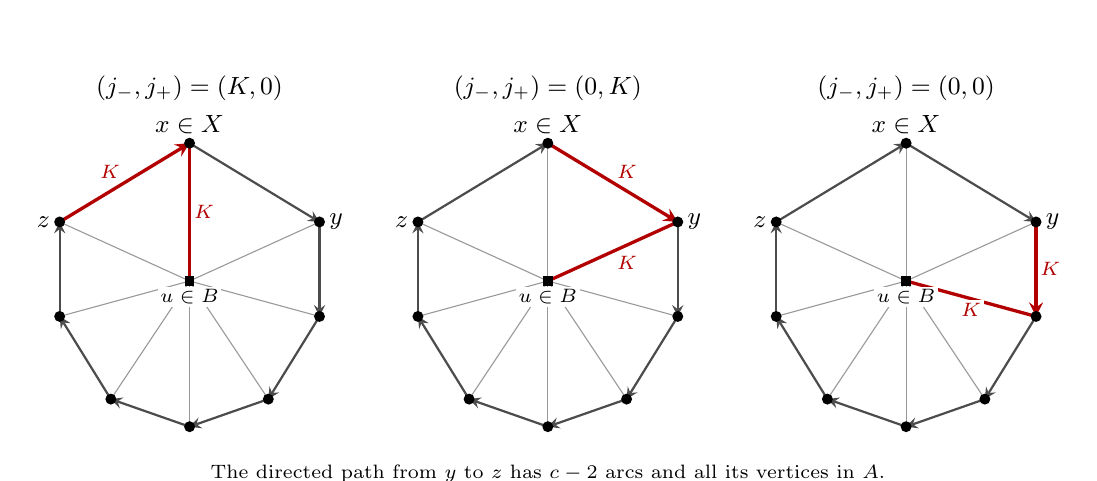
\begin{tikzpicture}[x=1cm,y=1cm,font=\small,>=stealth,
 rim/.style={circle,fill=black,inner sep=1.4pt},
 hub/.style={rectangle,fill=black,inner sep=1.7pt},
 arc/.style={->,black!70,thick},
 spoke/.style={black!40,thin},
 marked/.style={red!70!black,very thick},
 tag/.style={fill=white,inner sep=1pt,font=\scriptsize}]
\foreach \case/\offset/\jm/\jp in {1/2.1/K/0,2/6.65/0/K,3/11.2/0/0} {
\begin{scope}[shift={(\offset,0)}]
\node at (0,2.35) {$(j_-,j_+)=(\jm,\jp)$};
\coordinate (x) at (0,1.65);
\coordinate (y) at (1.65,.65);
\coordinate (v1) at (1.65,-.55);
\coordinate (v2) at (1,-1.6);
\coordinate (v3) at (0,-1.95);
\coordinate (v4) at (-1,-1.6);
\coordinate (v5) at (-1.65,-.55);
\coordinate (z) at (-1.65,.65);
\coordinate (u) at (0,-.1);
\foreach \v in {x,y,v1,v2,v3,v4,v5,z} {\draw[spoke] (u)--(\v);}
\draw[arc] (v1)--(v2);
\draw[arc] (v2)--(v3);
\draw[arc] (v3)--(v4);
\draw[arc] (v4)--(v5);
\draw[arc] (v5)--(z);
\ifnum\case=1
 \draw[arc,marked] (z)--node[tag,above left] {$K$} (x);
 \draw[arc] (x)--(y);\draw[arc] (y)--(v1);
 \draw[marked] (u)--node[tag,right] {$K$} (x);
\fi
\ifnum\case=2
 \draw[arc] (z)--(x);
 \draw[arc,marked] (x)--node[tag,above right] {$K$} (y);
 \draw[arc] (y)--(v1);
 \draw[marked] (u)--node[tag,below right] {$K$} (y);
\fi
\ifnum\case=3
 \draw[arc] (z)--(x);\draw[arc] (x)--(y);
 \draw[arc,marked] (y)--node[tag,right] {$K$} (v1);
 \draw[marked] (u)--node[tag,below] {$K$} (v1);
\fi
\foreach \v in {x,y,v1,v2,v3,v4,v5,z} {\node[rim] at (\v) {};}
\node[hub,label={[font=\scriptsize,fill=white,inner sep=1pt]below:$u\in B$}] at (u) {};
\node[above] at (x) {$x\in X$};
\node[right] at (y) {$y$};\node[left] at (z) {$z$};
\end{scope}
}
\node[font=\scriptsize] at (6.65,-2.55)
 {The directed path from $y$ to $z$ has $c-2$ arcs and all its vertices in $A$.};
\end{tikzpicture}
\caption{The three possibilities for completing the auxiliary rim at $x$,
illustrated with $c=8$. The assigned arcs are $z\to x$ and $x\to y$.
Marked arcs and spokes are labeled $K$; all others have type $0$.}
\label{fig:cover-down:marked-endpoint-completion}
\end{figure}


The degree bound on $\bigcup_iF_i$ implies that each endpoint
and each assigned hub occurs in at most $C_{\rm cov}\tau n$ pairs.
There are consequently $O_c(\tau n^2)$ internal vertex choices.
Let $f_X(v)$ count the previous choices of $v\in A$ as a new
internal path vertex in this construction, and put
$L_X(v):=f_X(v)+f_X(\pi^{-1}(v))$.
We choose $v$ only while $L_X(v),L_X(\pi(v))<\sqrt\tau n$.
Since $\sum_vL_X(v)=O_c(\tau n^2)$, this excludes at most
$C_{\rm cov}\sqrt\tau n$ candidates. The prescribed endpoints, fixed
hubs and free choices give $\Delta_*\le C_{\rm cov}\sqrt\tau n$
for the graph of internal edges in every partial union.
The previously used and reserved physical edges, including
$F_{\rm cov}$ and all endpoint spokes other than the two
reserved for the current pair, therefore exclude at most
another $C_{\rm cov}\sqrt\tau n$ candidates at each extension.
With $C_{\rm cov}$ chosen to include both losses, the hierarchy and order
threshold give $C_{\rm cov}\sqrt\tau n+\Lambda_{\rm sep}\le\beta_0a/2$.
Thus each extension is possible. Let $F_Z$ be the union of the
wheels obtained from the factors at $Z$, and $F_X$ the union of
the wheels completed from the endpoint assignments at $X$.
Then
\begin{equation*}
 F_U=F_{\rm ap}\cup F_{\rm cov}\cup F_Z\cup F_X,\qquad
 \Delta_*(F_U[A\cup B])
 \le \gamma_{\rm cov}n+C_{\rm cov}\sqrt\tau n\le\nu n\le\nu N.
\end{equation*}
The wheels at hubs in $Z$ cover $H_{\rm rem}[A,Z]$.
The endpoint assignments and their completed paths cover
$G_{\rm rem}[X,A]\cup H_{\rm rem}[X,B]$.
Together with \eqref{eq:completion:marked-boundary-remainder},
this proves
\eqref{eq:completion:active-output:marked}.
\end{proof}

\begin{localclaim}[The next divisible remainder]\label{clm:protected:restore:marked}
The remainder $\mathcal R':=\mathcal R-F_E-F_D-F_U$ is marked $c$-wheel-divisible,
is an extended subgraph of $\mathcal R[I\cup J]$, and satisfies
\eqref{eq:family:protected-output:marked}. In fact,
\begin{equation}
 E(\mathcal R[I\cup J]-\mathcal R')
 =E_{\rm del}\dot\cup E(F_U[I'\cup J']).
 \label{eq:completion:one-level-remainder:marked}
\end{equation}
\end{localclaim}

Figure~\ref{fig:cover-down:inner-edge-use} also shows where the
used edges lie inside $I\cup J$ in the marked case, with
the rim-arc endpoints interpreted as auxiliary endpoints.

\begin{proof}
The packings avoid $\mathcal K$, so $\mathcal K\subseteq\mathcal R'$.
Since $\mathcal R$ is marked $c$-wheel-divisible and each removed
wheel is a marked $c$-wheel, $\mathcal R'$ is marked $c$-wheel-divisible.
Claim~\ref{clm:protected:deep:marked} covers every edge of
$\mathcal Q_0$ incident with $T\cup W$, while the retained
graph $\mathcal K$ lies in $\mathcal R[I\cup J]$.
Claim~\ref{clm:protected:active:marked} covers every other
remaining edge outside $I'\cup J'$. Hence
$\mathcal R'\subseteq\mathcal R[I\cup J]$.
Within $I\cup J$, $F_E$ uses exactly $E_{\rm del}$, $F_D$ uses no edge,
and $F_U$ uses exactly $F_U[I'\cup J']$.
This proves \eqref{eq:completion:one-level-remainder:marked}.
The same identity gives
$\Delta_*(\mathcal R[I\cup J]-\mathcal R')
\le C_{\rm cov}\xi m+\nu N\le(C_{\rm cov}\xi+2\nu/\epsilon)m\le\gamma m/50<\gamma m$,
since $m\ge\epsilon N/2$, $C_{\rm cov}\xi\le\gamma/100$ and
$\nu=\gamma\epsilon/200$.
Among the edges of $\mathcal R[I\cup J]-\mathcal R'$, those
incident with $T\cup W$ are exactly $E_{\rm del}$, with
$\Delta_*(E_{\rm del})\le C_{\rm cov}\xi m\le\sigma m$.
Finally, $D[T\cup W]=\varnothing$ and
$F_U\subseteq\mathcal Q'[V'\cup U']$ give
$\mathcal R'[T\cup W]=\mathcal R[T\cup W]$.
When $T=W=\varnothing$, we have $I'=I$ and $J'=J$, and
$\mathcal K,E_{\rm del},F_E,F_D$ are empty. Thus
$\mathcal R'=\mathcal R-F_U$, where $F_U$ is the union of the wheels
supplied by Claim~\ref{clm:protected:active:marked}.
\end{proof}
Combining $\mathcal P_E$, $\mathcal P_D$ and the packing from
Claim~\ref{clm:protected:active:marked} proves the lemma.
\end{proof}

\section{Sampling estimates used in completion}
\label{subsec:completion:reference-estimates}
We establish simultaneous neighborhood and weighted-cycle estimates
for the ordinary and marked completion samples.

\subsection{Concentration of neighborhood intersections}
We first prove the concentration bounds used to supply the
neighborhood inequalities in the ordinary and marked cover-down lemmas
(Lemmas~\ref{lem:completion:ordinary-cover-down} and~\ref{lem:completion:marked-cover-down}).
In each application, the finite list of summation sets, patterns and
potential roots is fixed before sampling. A union bound gives the
estimates simultaneously for that list, allowing a root to be selected
from it after the sample is exposed.

\paragraph{Ordinary neighborhood counts.}
Let $V,U$ be disjoint finite sets, let $P,F$ be graphs on $V$, and let
$P_{\rm el}\subseteq P$ and $R\subseteq P_{\rm el}$. Let $H$ be bipartite on $(V,U)$.
Let $q,s\in[0,1]$, and let $X\subseteq V$ and $Y\subseteq U$.
For $\varnothing\ne A\subseteq X$, $S\subseteq X$ and
$J\subseteq Y$, let
\begin{equation}
 N_V^{\rm ord}(A;S,J):=|A\cap N_R(S)\cap N_H(J)|,\qquad
 \mu_V^{\rm ord}(A;S,J):=q^{|S|}s^{|J|}|A\cap N_{P_{\rm el}}(S)|.
\label{eq:cn:ordinary-row-count}
\end{equation}
For $\varnothing\ne B\subseteq Y$ and $F$-independent $S\subseteq X$, let
\begin{equation}
 N_U^{\rm ord}(B;S):=|B\cap N_H(S)|,\qquad
 \mu_U^{\rm ord}(B;S):=s^{|S|}|B|.
 \label{eq:cn:ordinary-index-count}
\end{equation}
Empty intersections are their ambient part, and every zeroth power
is one, including $0^0$.

\paragraph{Neighborhood counts with prescribed edge types.}
Let $V,U$ be disjoint finite sets, let $P,F$ be graphs on $V$, and let
$\pi:V\to V$ be a permutation. Let $R^0,R^K$ be digraphs on $V$,
and let $H^0,H^K$ be edge-disjoint bipartite graphs with parts $V,U$.

Let $p_0,p_K\in[0,1]$ be directional density parameters,
let $s_0,s_K:U\to[0,1]$, and let
$X\subseteq V$, $Y\subseteq U$.

We define the sets of possible neighbors for the two arc types by
\begin{equation*}
\begin{array}{c|cc}
 &M_\tau^+(x)&M_\tau^-(x)\\\hline
 \tau=0&N_P(x)&N_P(x)\\
 \tau=K&\pi^{-1}(N_P(x))&N_P(\pi(x)).
\end{array}
\end{equation*}

Let $E_0,E_K\subseteq\{(u,v):\{u,v\}\in E(P)\}$ be fixed sets
of directed physical edges of each type. We define the ordered physical arcs
\begin{equation*}
a_{0,+}(x,z):=(x,z),\quad a_{0,-}(x,z):=(z,x),\quad
 a_{K,+}(x,z):=(x,\pi(z)),\quad a_{K,-}(x,z):=(z,\pi(x)).
\end{equation*}

Let $M_{\tau,\rm el}^e(x):=\{z\in M_\tau^e(x):a_{\tau,e}(x,z)\in E_\tau\}$.
The prescribed sets of physical arcs satisfy
\begin{equation*}
 x\to y\in E(R^0)\ \Longrightarrow\ (x,y)\in E_0,\qquad
 x\to y\in E(R^K)\ \Longrightarrow\ (x,\pi(y))\in E_K.
\end{equation*}

\paragraph{Marked neighborhood counts over $A$.}
Let $\varnothing\ne A\subseteq X$. For $\tau\in\{0,K\}$ and
$e\in\{+,-\}$, fix sets $S_\tau^e,T_\tau^e\subseteq X$, and
fix disjoint sets $J_0,J_K\subseteq Y$.
The sets $S_\tau^e$ specify roots of neighborhoods in $R^\tau$,
whereas the roots $y\in T_\tau^e$ specify the sets $M_\tau^e(y)$
determined by $P$ and $\pi$.
We collect these sets in the neighborhood pattern
$i:=((S_\tau^e,T_\tau^e)_{\tau,e},J_0,J_K)$ and put
$k_\tau:=|S_\tau^+|+|S_\tau^-|$.
We define
\begin{equation}
\begin{split}
 A_i^\circ:=\{z\in A:\;&a_{\tau,e}(x,z)\in E_\tau
       \text{ for every }\tau,e,\ x\in S_\tau^e,\\
 &\text{the underlying undirected edges of these arcs are pairwise distinct}\}.
\end{split}
\label{eq:cn:admissible-outer-set}
\end{equation}
For $\mathcal Q=(R^0,R^K,H^0,H^K)$, let
\begin{equation}
\begin{aligned}
 N_V^{\rm mark}(A;i)&:=
 \left|A_i^\circ\cap\bigcap_{\tau,e}
 \left(\bigcap_{x\in S_\tau^e}N_{R^\tau}^e(x)\cap\bigcap_{y\in T_\tau^e}M_\tau^e(y)\right)
 \cap N_{H^0}(J_0)\cap N_{H^K}(J_K)\right|,\\
 \mu_V^{\rm mark}(A;i)&:=
 p_0^{k_0}p_K^{k_K}\prod_{u\in J_0}s_0(u)\prod_{u\in J_K}s_K(u)\cdot\left|A_i^\circ\cap\bigcap_{\tau,e}\left(\bigcap_{x\in S_\tau^e}M_{\tau,\rm el}^e(x)\cap\bigcap_{y\in T_\tau^e}M_\tau^e(y)\right)\right|.
\end{aligned}
\label{eq:cn:marked-row-count}
\end{equation}

\paragraph{Marked neighborhood counts over $B$.}
Let $\varnothing\ne B\subseteq Y$. For disjoint $S_0,S_K\subseteq X$
with $F$-independent union, we define
\begin{equation}
N_U^{\rm mark}(B;S_0,S_K):=|B\cap N_{H^0}(S_0)\cap N_{H^K}(S_K)|,\qquad \mu_U^{\rm mark}(B;S_0,S_K):=\sum_{u\in
B}s_0(u)^{|S_0|}s_K(u)^{|S_K|}.
\label{eq:cn:marked-index-count}
\end{equation}
Empty intersections and zeroth powers
have the same conventions as for ordinary counts.

The set $A_i^\circ$ can be empty. For example, if
$x\in S_0^-$ and $\pi^{-1}(x)\in S_K^-$, then $a_{0,-}(x,z)=(z,x)=a_{K,-}(\pi^{-1}(x),z)$ for all $z\in A$. The
two required arcs have the same underlying edge, so
$A_i^\circ=\varnothing$ and
$N_V^{\rm mark}(A;i)=\mu_V^{\rm mark}(A;i)=0$.


For the raw interval sample of
Definition~\ref{def:four:local-interval-law}, recall that
$\mathcal X_u^g$ is the family of intervals of color $g$ at hub $u$.
The assignment $\sigma_{\mathcal X}$ in
\eqref{eq:interval:assignment} gives color $g$ to $xu$ when
$x$ lies in an interval of $\mathcal X_u^g$.
Outside the union of the extended intervals $I\cup\{I^+\}$ with
$I\in\bigcup_g\mathcal X_u^g$, it uses the independent label color
$B_{u,x}$. At the terminal successor of each interval in these
families, its value is $\bot$.

\begin{lemma}
\label{lem:pr:rt1-realisation}
Let $h\ge0$ and $d\ge2$ be integers. There is $c_{h,d}>0$ such that
the following holds for every $\varepsilon>0$.
Let $V,U$ be finite disjoint sets, let $P$ be a graph on $V$, and let
$\pi$ be a permutation of $V$ with $L_\pi>10d$.
Let $F$ be a graph on $V$ containing every distinct pair at $\pi$-distance at most $3d$,
and let $P_{\rm el}\subseteq P$ and $q\in[0,1]$.

Let $\sigma_{\mathcal X}$ be the assignment in
\eqref{eq:interval:assignment} for a raw interval sample on
$(V,U,\pi)$ with parameter $d$, interval colors $\Gamma=\{1,2\}$,
label colors $\Sigma=\mathcal J$, and functions
$q_1,q_2,(\widetilde s_j)_{j\in\mathcal J}$. Suppose that
$\widetilde s_{j_0}(u)=s$ for every $u\in U$, for a fixed
$j_0\in\mathcal J$ and $s\in[0,1]$, and put
$E(H):=\{xu:\sigma_{\mathcal X}(xu)=j_0\}$.
Let $R$ be the random spanning subgraph of $P_{\rm el}$ whose edges
are present independently with probability $q$, independently of all pair variables.

Let $\mathcal I$ index a finite list of instances of
\eqref{eq:cn:ordinary-row-count} with $|S|+|J|\le h$,
or \eqref{eq:cn:ordinary-index-count} with $|S|\le h$,
with the list and all its summation sets and roots specified before sampling.
For an instance $i$ of $N_V^{\rm ord}$, let $N_i,\mu_i$ denote
$N_V^{\rm ord},\mu_V^{\rm ord}$ evaluated at its prescribed sets and roots,
with $a_i:=|A_i|$. For an instance of $N_U^{\rm ord}$, they denote
$N_U^{\rm ord},\mu_U^{\rm ord}$ instead, with $a_i:=|B_i|$.

Then, for $\mathcal B:=(R,H)$,
\begin{equation*}
 \mathbb E N_i(\mathcal B)=\mu_i\quad(i\in\mathcal I),\qquad
 \Pr\bigl(\exists i\in\mathcal I:
 |N_i(\mathcal B)-\mu_i|>\varepsilon a_i\bigr)
 \le\sum_{i\in\mathcal I}2e^{-c_{h,d}\varepsilon^2a_i}.
\end{equation*}
\end{lemma}
\begin{proof}
The raw assignment is determined by independent activation,
start-color and label-color variables. The count
$N_V^{\rm ord}(A_i;S,J)$ is a sum of membership indicators over
$z\in A_i$. For $z\in A_i\cap N_{P_{\rm el}}(S)$, the
required spokes have distinct hubs, and the required rim edges are
distinct. The spoke assignments at these hubs are independent of
one another and of the physical-edge trials, so their probabilities
multiply to give the corresponding summand of $\mu_i$.
The count $N_U^{\rm ord}(B_i;S)$ is a sum over $u\in B_i$. Its prescribed labels are
$F$-independent and hence have pairwise $\pi$-distance greater than
$3d$. Their determining interval coordinates are disjoint. This
again gives $\mathbb E N_i=\mu_i$.

For a constant $K_{h,d}\ge1$, each summand uses at most $K_{h,d}$
coordinates and each coordinate changes at most $K_{h,d}$ summands.
Indeed, an interval coordinate affects at most $3d+1$ labels at
one hub, and a rim edge has two endpoints. Thus at most
$K_{h,d}a_i$ coordinates affect $N_i$, each with change bound
$K_{h,d}$. A count with no such coordinates is constant. Otherwise
McDiarmid's bounded-differences inequality (Theorem~\ref{thm:prelim:bounded-differences}) gives
$2\exp(-2\varepsilon^2a_i/K_{h,d}^3)$ as its failure bound.
We take $c_{h,d}:=2/K_{h,d}^3$ and sum over $i$.
\end{proof}

\Needspace{8\baselineskip}
\begin{lemma}
\label{lem:pr:marked-realisation}
Let $h\ge0$ and $d\ge2$ be integers. There is $c_{h,d}>0$ such that
the following holds for every $\varepsilon>0$.
Let $V,U$ be finite disjoint sets, let $P$ be a graph on $V$, and let
$\pi$ be a permutation of $V$ with $L_\pi>10d$.
Let $F$ be a graph on $V$ containing every distinct pair at $\pi$-distance at most $3d$.

Let $\sigma_{\mathcal X}$ be the assignment in
\eqref{eq:interval:assignment} for a raw interval sample on
$(V,U,\pi)$ with parameter $d$, interval colors $\Gamma=\{1,2\}$,
label colors $\Sigma=\mathcal J$, and functions
$q_1,q_2,(\widetilde s_j)_{j\in\mathcal J}$.
Let $j_0\in\mathcal J$ and $g_0\in\{1,2\}$, and let
$s_0:=\widetilde s_{j_0}$, $s_K:=q_{g_0}$,
$E(H^0):=\{xu:\sigma_{\mathcal X}(xu)=j_0\}$ and
$E(H^K):=\{xu:\sigma_{\mathcal X}(xu)=g_0\}$.

Let
$E_0,E_K\subseteq\{(x,y):\{x,y\}\in E(P)\}$ and
$p_0,p_K\in[0,1]$. For $j\in\{0,K\}$ and $e\in E(P)$, let
$m_j(e):=|\{(x,y)\in E_j:\{x,y\}=e\}|$.
Assume $m_0(e)p_0+m_K(e)p_K\le1$ for all $e\in E(P)$. If $p_K>0$,
suppose $(x,\pi(x))\notin E_K$ for every $x\in V$.

Let $(C_e)_{e\in E(P)}$ be independent random variables,
independent of all pair variables. For each $e\in E(P)$, the distribution
of $C_e$ assigns probability $p_j$ to each state $(x,y,j)$ with
$(x,y)\in E_j$ and $\{x,y\}=e$, and the remaining mass to $\bot$.
Let
\begin{equation*}
\begin{aligned}
 E(R^0)&:=\{x\to y:C_{\{x,y\}}=(x,y,0)\},\\
 E(R^K)&:=\{x\to\pi^{-1}(y):C_{\{x,y\}}=(x,y,K)\},
\end{aligned}
\end{equation*}
and $\mathcal B:=(R^0,R^K,H^0,H^K)$.

Let $\mathcal I$ index a finite list of instances of
\eqref{eq:cn:marked-row-count} with
$\sum_{\tau,e}(|S_\tau^e|+|T_\tau^e|)+|J_0|+|J_K|\le h$,
or \eqref{eq:cn:marked-index-count} with $|S_0|+|S_K|\le h$,
with the list and all its summation sets, patterns and roots specified before sampling.
For an instance $i$ of $N_V^{\rm mark}$, let $N_i,\mu_i$ denote
$N_V^{\rm mark},\mu_V^{\rm mark}$ evaluated at its prescribed sets and pattern,
with $a_i:=|A_i|$. For an instance of $N_U^{\rm mark}$, they denote
$N_U^{\rm mark},\mu_U^{\rm mark}$ instead, with $a_i:=|B_i|$.

Then
\begin{equation*}
 \mathbb E N_i(\mathcal B)=\mu_i\quad(i\in\mathcal I),\qquad
 \Pr\bigl(\exists i\in\mathcal I:
 |N_i(\mathcal B)-\mu_i|>\varepsilon a_i\bigr)
 \le\sum_{i\in\mathcal I}2e^{-c_{h,d}\varepsilon^2a_i}.
\end{equation*}
\end{lemma}

The proof is analogous to that of Lemma~\ref{lem:pr:rt1-realisation} and is given in Appendix~\ref{app:proof:lem-pr-marked-realisation}.
%The proof uses bounded differences on the raw interval variables and one state variable for each physical edge. The ordinary proof above gives the corresponding calculation without edge types.



\subsection{Ordinary sampling estimates}
The next two lemmas give estimates for the ordinary completion sample
used in Proposition~\ref{prop:completion:ordinary-construction}.
The rim and spoke load operators are defined in
Section~\ref{sec:four:relative-weights}.
Lemma~\ref{lem:completion:ordinary-reference} supplies the weights and
configuration counts needed for the deterministic correction and
packing results. Lemma~\ref{lem:completion:ordinary-reference-cuts}
supplies the large-cut bounds needed for the divisibility corrections
on the packing and inner pairs.

We use the conflict graph $F_{\pi,3d}$, whose edges join distinct
vertices at $\pi$-distance at most $3d$. The coefficient and deterministic
incidence-change bounds below are independent of $d$; the order
thresholds and concentration rates may depend on $d$. For triangles,
$\vartheta\ge\delta_{C_3}\ge3/4$ by Proposition~\ref{prop:four:lower}.
This lower bound supplies the common paths used in the proof.

\Needspace{8\baselineskip}

\paragraph{Spoke probabilities and independence in the ordinary sample.}
For an ordinary completion sample $(R_0,H_0)$ on $(P,V,U,\pi)$,
let $n:=|V|$, $p_R:=\varrho s$ and $p_H:=s$.
Lemma~\ref{lem:interval:raw-law} gives the following facts.
\begin{enumerate}[label=\textup{(S\arabic*)}]
\item\label{item:ordinary-law:S1} The pair-state vectors at distinct
hubs are independent of one another and of the physical-edge trials.
\item\label{item:ordinary-law:S2} For every $v\in V$ and $u\in U$,
$\Pr(vu\in E(H_0))=p_H=s$. At a fixed hub, the states on any
$(3d,\pi)$-separated set of vertices are independent.
\end{enumerate}

\paragraph{From cycle weights to wheel weights.}
Let $r\ge3$, $\vartheta\ge\max\{1/2,\delta_{C_r}\}$ and $\alpha>0$.
Let $P$ be a sufficiently large graph on $V$, $|V|=n$, with
$\delta(P)\ge(\vartheta+\alpha)n$. Let $\lambda:\mathcal C_r(P)\to\mathbb R_{\ge0}$ be a fixed positive bounded
fractional cycle weighting supplied by Theorem~\ref{thm:four:dense-spread},
depending only on $P$, with
\begin{equation}
 \sum_{C\ni e}\lambda(C)=1,
 \quad B_P^{-1}n^{2-r}\le\lambda(C)\le B_Pn^{2-r},
 \quad \sum_{C\ni v}\lambda(C)=\frac{d_P(v)}2,
 \label{eq:family:OF.A11}
\end{equation}
for every $e\in E(P)$, $C\in\mathcal C_r(P)$ and $v\in V$, where
$B_P>1$ depends only on $r,\vartheta,\alpha$.
For a graph $\mathcal F$ on $V$, a disjoint set $U$ of size $m>0$,
and $p_R,p_H>0$, let
\begin{equation*}
 \mathcal W_P:=\{W(C,u):C\in\mathcal C_r(P),\ u\in U,
                            E(\mathcal F[V(C)])=\varnothing\}.
\end{equation*}
We define $\omega_0:\mathcal W_P\to\mathbb R_{>0}$ by
\begin{equation}
 \omega_0(W(C,u))
 :=\frac{\lambda(C)}{m p_R^{r-1}p_H^r}.
 \label{eq:family:OF.A12}
\end{equation}
For an ordinary extended graph $(Q,H)$, we recall the three sums in
\eqref{eq:loads:ordinary-potential-seed}--\eqref{eq:loads:ordinary-potential-transfers}.
The sum $\widehat L_e(Q,H;\omega_0)$ gives weight $\omega_0(W)$ to
each candidate wheel containing $e$ whose other edges lie in $(Q,H)$.
The quantity $\widehat I_{xy}(Q,H)$ is $n^{1-k}$ times the number
of pairs $(u,S)$ with $S\in\mathcal S_P(xy)$,
$E(P[S])\setminus\{xy\}\subseteq E(Q)$ and $S\subseteq N_H(u)$.
Here $S$ is a $k$-set containing $x,y$ with
$E(\mathcal F[S])=\varnothing$ and $\delta(P[S])\ge(\vartheta+\alpha/4)k$.
Finally, $\widehat T_{v,u,u'}(Q,H)$ is $n^{-r^2}$ times the number
of labeled configurations consisting of an ordered base $r$-cycle
and, for each base vertex $x$, an ordered $(r-1)$-vertex path $P_x$
such that $vP_xv$ and $xP_xx$ are both $r$-cycles.
Their $r^2$ free vertices are distinct, avoid $v$, are together
with $v$ independent in $\mathcal F$, and are adjacent in $H$ to
both hubs. All required rim edges lie in $Q$.
This last count does not require $vu$ or $vu'$ to belong to $E(H)$.

\Needspace{8\baselineskip}
\begin{lemma}
\label{lem:completion:ordinary-reference}
Let $r\ge3$, $\vartheta\ge\max\{1/2,\delta_{C_r}\}$, and
$\alpha,\omega_*,p_*>0$ be fixed.

There are an integer
$k\ge\max\{r+2,m_0(r,\alpha/4)\}$ and constants $\beta>0$ and $B_{\omega}>1$, depending only
on $r,\vartheta,\alpha,\omega_*,p_*$, where $m_0$ is from
Lemma~\ref{lem:four:edge-isolator}, with the following property.
Let $0<\eta_*\le1$ and
\begin{equation*}
 0<\varepsilon_0\ll\eta_*,1/r,\vartheta,\alpha,
 \omega_*,p_*,1/k,\beta,1/B_{\omega},1.
\end{equation*}
For every integer $d\ge2$, there are $n_0\in\mathbb N$,
$C_{\rm prob},c_{\rm prob}>0$ and $K_{\rm prob}\ge0$ such that the
following holds for $n\ge n_0$. The probability constants depend
only on $r,\vartheta,\alpha,\omega_*,p_*,\eta_*,d$. Let $P$ be a graph on $V$, let $U$ be disjoint
from $V$, and let $|V|=n$, $|U|=m$.
Let $(R_0,H_0)$ be an ordinary completion sample on $(P,V,U,\pi)$
with parameters $\varrho,s,d,(a_u),(b_u)$.
Let $\mathcal F:=F_{\pi,3d}$, $P^{\rm adm}:=P-E(\mathcal F)$,
$p_R:=\varrho s$, $p_H:=s$ and $D_0:=\frac{2m}{\varrho}$. Assume
$\omega_*n\le m\le n$, $p_R,p_H\in[p_*,1]$, $n/2\le D_0\le2n$,
$\delta(P)\ge(\vartheta+\alpha)n$ and $d_P(v)=D_0\pm \varepsilon_0n$ for all $v\in V$. Let $\lambda$ and $\omega_0$ be the fixed cycle and wheel weightings
on $\mathcal C_r(P)$ and $\mathcal W_P$, respectively, in
\eqref{eq:family:OF.A11}--\eqref{eq:family:OF.A12}.
Then $B_{\omega}^{-1}n^{1-r}\le\omega_0(W)\le B_{\omega}n^{1-r}$ for every
$W\in\mathcal W_P$.

Let $\mathcal E_{\rm ord,full}$ be the event that
$d_{H_0}(v)\ge\beta n$ for every $v\in V$ and
\begin{equation}
\begin{aligned}
	\widehat L_e(R_0,H_0;\omega_0)&=1\pm \eta_* &&(e\in E(P^{\rm adm})\dot\cup(V\times U)),\\
	\widehat I_{xy}(R_0,H_0)&\ge\beta &&(xy\in E(P^{\rm adm})),\\
	\widehat T_{v,u,u'}(R_0,H_0)&\ge\beta &&(v\in V,\ u,u'\in U,\ u\ne u').
\end{aligned}
\end{equation}
Then
\begin{equation}\label{eq:prob:lem:reference:ordinary-numerical}
	\Pr(\mathcal E_{\rm ord,full}^c) \le C_{\rm prob}n^{K_{\rm prob}}e^{-c_{\rm prob}n^{1/5}}\le n^{-10}.
\end{equation}
\end{lemma}

\paragraph{Independent coordinates for the ordinary sample.}
The variables in the raw interval sample of
Definition~\ref{def:four:local-interval-law} give the following bound,
used in the concentration arguments for
Lemmas~\ref{lem:completion:ordinary-reference} and
\ref{lem:completion:ordinary-reference-cuts}.
\begin{enumerate}[label=\textup{(S\arabic*)},start=3]
\item\label{item:ordinary-law:S3} The states at each hub depend on
at most $3n$ independent finite-valued coordinates. Each state is
determined by at most $3d+1$ activation variables, $d+1$ start-color
variables and one label-color variable. Changing one variable of
these types affects at most $3d+1$ states, $d+1$ states and one state, respectively.
Thus $B:=4d+3$ bounds both the number of coordinates determining
one state and the number of states affected by one coordinate.
\end{enumerate}

\begin{proof}[Proof of Lemma~\ref{lem:completion:ordinary-reference}]
We choose $k\ge\max\{r+2,m_0(r,\alpha/4)\}$ with
$1/k\ll\alpha,1/r$. The constants $\beta,B_{\omega}$ specified below
depend only on $r,\vartheta,\alpha,\omega_*,p_*$ and precede
$\eta_*,\varepsilon_0,d$. Put $L:=6d$, $B:=4d+3$ and
$(Q,H):=(R_0,H_0)$. We use the sampling properties
\ref{item:ordinary-law:S1}--\ref{item:ordinary-law:S3}.

\paragraph{Potential edge loads.}
Equation~\eqref{eq:family:OF.A12} gives the coefficient bounds with
$B_{\omega}:=B_P\max\{1,(\omega_*p_*^{2r-1})^{-1}\}$.
For $e\in E(P^{\rm adm})\dot\cup(V\times U)$, put
$Z_e:=\widehat L_e(R_0,H_0;\omega_0)$.
For a rim root $e$, the remaining indicators have joint probability
$p_R^{r-1}p_H^r$; for a spoke root $vu$, it is $p_R^rp_H^{r-1}$.
These are unconditional probabilities of the products with the
root indicator omitted, by \ref{item:ordinary-law:S1} and
\ref{item:ordinary-law:S2}.

Since $\Delta(\mathcal F)\le L$, the cycles containing a forbidden
pair number $O_r(Ln^{r-3})$ through a fixed
$e\in E(P^{\rm adm})$, and $O_r(Ln^{r-2})$ through a fixed vertex.
The bound $\lambda(C)\le B_Pn^{2-r}$ makes their total weights
$O(L/n)$ and $O(L)$, respectively, also for $r=3$.
Thus \eqref{eq:family:OF.A11} gives $\mathbb EZ_e=1+O(L/n)$
for rim roots, and
\begin{equation}
 \mathbb EZ_{vu}=\frac{p_Rd_P(v)}{2mp_H}+O(L/n)
 =\frac{d_P(v)}{D_0}+O(L/n)=1\pm O(\varepsilon_0+L/n).
 \label{eq:family:OF.A15}
\end{equation}

For each additional rim edge or spoke, we bound the sum of
$\omega_0(W)$ over candidate wheels containing it and the prescribed root.
For a spoke root $vu$, this sum is $O(1/n)$ for each of the $O(n)$
other spokes at $u$ and rim edges incident with $v$, and $O(1/n^2)$
for every other rim edge or spoke. For a rim root $xy$, it is
$O(1/n)$ for each additional rim edge incident with $x$ or $y$
and each spoke at $x$ or $y$, and $O(1/n^2)$ for every other rim
edge or spoke. These bounds follow by fixing one or two further
labels, with constants independent of $d$.
Lemma~\ref{lem:pr:wi-interactions}, with $a=n$ and $B=4d+3$, therefore gives a sum of squared bounded-difference constants at most $C_B/n$.
By McDiarmid's bounded-differences inequality (Theorem~\ref{thm:prelim:bounded-differences}),
\begin{equation*}
 \Pr\bigl(\max_e|Z_e-\mathbb EZ_e|>n^{-1/8}\bigr)
 \le C_{\rm tail}n^2e^{-c_Bn^{3/4}}.
\end{equation*}
On its complementary event, \eqref{eq:family:OF.A15} gives
$\max_e|Z_e-1|\le C_0\varepsilon_0+O(L/n)+n^{-1/8}\le\eta_*$
by the hierarchy, with $n_0$ chosen after $d$.
Here, $C_0$ and the constant in $O(L/n)$ are independent of $d$,
and the maximum includes roots absent from $(R_0,H_0)$.

\paragraph{Spoke neighborhoods.}
For $J\subseteq U$ with $j=|J|\in\{1,2\}$, put
$T_J:=\bigcap_{u\in J}N_{H_0}(u)$.
The expectations of $|T_J|$ and $d_P(v;T_J)$ are
$p_H^jn$ and $p_H^jd_P(v)$ for every $v\in V$.
Each uses $O(n)$ independent variables determining the spoke
assignments at the hubs $u\in J$, and one variable changes at most
$B$ summands.
Also $\mathbb Ed_{H_0}(v)=p_Hm$, and, for distinct $x,y$ with
$xy\notin E(\mathcal F)$,
$\mathbb E|N_{H_0}(x)\cap N_{H_0}(y)|=p_H^2m$.
For these last two quantities the summands at distinct hubs are
independent. McDiarmid's bounded-differences inequality (Theorem~\ref{thm:prelim:bounded-differences}) with deviation $n^{7/8}$ and
a union bound give an event $\mathcal E_H$, determined by $H_0$,
with $\Pr(\mathcal E_H^c)\le C_{\rm tail}n^3e^{-c_Bn^{3/4}}$, on which all
these estimates hold. In particular, for large $n$,
\begin{equation}
 |T_J|\ge p_*^2n/2,\qquad
 d_P(v;T_J)\ge(\vartheta+\alpha/2)|T_J|
 \quad(J\in\tbinom U1\cup\tbinom U2,\ v\in V),
 \label{eq:family:OF.A8}
\end{equation}
and $d_{H_0}(v)\ge p_*\omega_*n/2$, while
\begin{equation}
 |N_{H_0}(x)\cap N_{H_0}(y)|
 =p_H^2m\pm n^{7/8}\ge c_3n,
 \qquad c_3:=p_*^2\omega_*/2.
 \label{eq:family:OF.A10}
\end{equation}
The degree estimates in \eqref{eq:family:OF.A8} include $v\notin T_J$.
Avoiding any bounded set of chosen labels and their
$\mathcal F$-neighbors excludes only $O(L+1)$ further labels.

\paragraph{Dense sets for the rim correction.}
Fix an outcome in $\mathcal E_H$. For $e=xy\in E(P^{\rm adm})$
and $u\in U$, put
$\mathcal S_{e,u}:=\{S\in\mathcal S_P(e):
S\setminus\{x,y\}\subseteq N_{H_0}(u)\}$, where
$\mathcal S_P(e)$ is defined in
\eqref{eq:loads:ordinary-potential-isolators}.
Sampling $k-2$ free vertices from $N_{H_0}(u)\setminus\{x,y\}$,
\eqref{eq:family:OF.A8} and the hypergeometric Chernoff bound
(Lemma~\ref{lem:prelim:chernoff}) give probability
at least $3/4$ that $\delta(P[S])\ge(\vartheta+\alpha/4)k$.
The prescribed vertices $x,y$ and integer rounding change the
relevant degree expectations by $O(1)$. The sum of the degree-failure
probabilities is therefore at most $k e^{-c_\alpha k}$.
For a sampled vertex, the estimate is conditional on its inclusion
and is summed with its inclusion probability.
The initial choice of $k$ makes this sum less than $1/4$.
Requiring $E(\mathcal F[S])=\varnothing$ excludes only
$O_k(Ln^{k-3})$ sets, since $xy\notin E(\mathcal F)$.
Hence $|\mathcal S_{e,u}|\ge c_1n^{k-2}$ for $c_1>0$
independent of $d$. Neither $xu$ nor $yu$ is required to belong to $H_0$.

Write $I_f:=\ind_{\{f\in E(R_0)\}}$ and define
\begin{equation*}
 N_{e,u}:=\sum_{S\in\mathcal S_{e,u}}
          \prod_{f\in E(P[S])\setminus\{e\}}I_f,
 \qquad J_{e,u}:=n^{2-k}N_{e,u}.
\end{equation*}
Conditionally on $H_0$, the physical-edge trials are independent, so
$\mathbb E(N_{e,u}\mid H_0)\ge2c_2n^{k-2}$ with
$c_2:=c_1p_*^{\binom{k}{2}-1}/2$.
Changing $I_f$ affects $O_k(n^{k-3})$ summands when
$f\cap\{x,y\}\ne\varnothing$ and $O_k(n^{k-4})$ otherwise.
$I_e$ does not occur. The sum of squared bounded-difference constants is
$O_k(n^{2k-5})$. Conditional on $H_0$, McDiarmid's bounded-differences inequality (Theorem~\ref{thm:prelim:bounded-differences})
gives failure probability at most $2e^{-c_4n}$ for
$N_{e,u}\ge c_2n^{k-2}$.
After a union bound over at most $n^3$ pairs $(e,u)$,
\begin{equation}
 \widehat I_e(R_0,H_0)
 =\frac1n\sum_{u\in U}\ind_{\{xu,yu\in E(H_0)\}}J_{e,u}
 \ge c_2c_3
 \quad(e=xy\in E(P^{\rm adm})),
\end{equation}
by \eqref{eq:family:OF.A10}. This bound also includes $e\notin E(R_0)$.

\paragraph{Configurations for spoke transfer.}
Still conditional on $H_0\in\mathcal E_H$, fix $v\in V$ and
distinct $u,u'\in U$, and put $T:=N_{H_0}(u)\cap N_{H_0}(u')$.
A configuration in $\mathcal T_P(v;u,u')$ with all its free-label
spokes in $H_0$ consists of an $r$-cycle $C$ in $P[T\setminus\{v\}]$
and, for each $x\in V(C)$, an ordered path $P_x$ on $r-1$ vertices
of $T$ such that $vP_xv$ and $xP_xx$ are cycles.
The sets $\{v\},V(C),(V(P_x))_{x\in V(C)}$ are pairwise disjoint,
and their union is independent in $\mathcal F$.

For $r\ge4$, \eqref{eq:family:OF.A8} gives degrees into $T$
exceeding $|T|/2$ by a fixed margin. We choose the two endpoints of
$P_x$ in $N_P(v;T)\cap N_P(x;T)$ and join them by a path of
length $r-2$, choosing its last internal vertex in a common
neighborhood. There are $\Omega(n^{r-1})$ choices.
For $r=3$, the degree bound is $(3/4+\alpha/2)|T|$.
The common neighborhood of $v,x$ has size at least
$(1/2+\alpha)|T|$, and its induced minimum degree is at least
$(1/4+3\alpha/2)|T|$. Its $\Omega(n^2)$ ordered adjacent pairs
are the required paths $P_x$.
The base cycle has $\Omega(n^r)$ choices by successive neighbor
choices and a final common-neighbor choice.
Avoiding used labels and their $\mathcal F$-neighbors at each step
therefore leaves at least $c_5n^{r+r(r-1)}=c_5n^{r^2}$
configurations, with $c_5>0$ independent of $d$.

Let $M_{v,u,u'}:=n^{r^2}\widehat T_{v,u,u'}(R_0,H_0)$, with the
two root spokes omitted as in
\eqref{eq:loads:ordinary-potential-transfers}.
Each configuration requires at most $2r^2+r$ distinct physical
edges. Its indicator product contains one factor for each such
edge, including any edge shared by its constituent cycles.
Thus $\mathbb E(M_{v,u,u'}\mid H_0)\ge2c_6n^{r^2}$ for
$c_6:=c_5p_*^{2r^2+r}/2$.
A physical edge at $v$ fixes one free label and affects
$O_r(n^{r^2-1})$ configurations; any other edge fixes two and
affects $O_r(n^{r^2-2})$. The sum of squared bounded-difference constants is
$O_r(n^{2r^2-1})$. McDiarmid's bounded-differences inequality (Theorem~\ref{thm:prelim:bounded-differences}) and a union bound over
$O(n^3)$ triples give conditional failure at most $C_{\rm tail}n^3e^{-c_7n}$
for $\widehat T_{v,u,u'}\ge c_6$ simultaneously, without requiring
$vu,vu'\in E(H_0)$.

We choose $\beta\le\min\{p_*\omega_*/2,c_2c_3,c_6\}$, before
$\eta_*$ and $d$.
Averaging the conditional failure bounds for $\widehat I_e$ and
$\widehat T_{v,u,u'}$ over outcomes in $\mathcal E_H$, and adding
$\Pr(\mathcal E_H^c)$ and the failure probability for the estimates on
$\widehat L_e$, gives
\begin{equation*}
 \Pr(\mathcal E_{\rm ord,full}^c)
 \le C_{\rm tail}n^3\bigl(e^{-c_Bn^{3/4}}+e^{-c_4n}+e^{-c_7n}\bigr).
\end{equation*}
This implies \eqref{eq:prob:lem:reference:ordinary-numerical} with
the stated dependencies, uniformly over the marginal arrays.
\end{proof}

\Needspace{8\baselineskip}
\begin{lemma}
\label{lem:completion:ordinary-reference-cuts}
Let $0<\alpha<1/2$ and $\omega_*,p_*>0$.
There are $0<\delta_c<1/4$ and $h>0$, depending only on
$\alpha,\omega_*,p_*$, such that the following holds.
For every integer $d\ge2$, there are $n_0\in\mathbb N$,
$C_{\rm prob},c_{\rm prob}>0$ and $K_{\rm prob}\ge0$, depending only
on $\alpha,\omega_*,p_*,d$, such that the following holds for $n\ge n_0$. Let $V,U$ be disjoint, with $|V|=n$ and
$\omega_*n\le|U|\le n$, and let $P$ be a graph on $V$ with
$\delta(P)\ge(1/2+\alpha)n$.
Let $(R_0,H_0)$ be an ordinary completion sample on $(P,V,U,\pi)$
with parameters $\varrho,s,d,(a_u),(b_u)$.
Let $\mathcal F:=F_{\pi,3d}$, $P^{\rm adm}:=P-E(\mathcal F)$ and
$p_R:=\varrho s$, $p_H:=s$, and assume $p_R,p_H\ge p_*$.
Let $\vec P^{\rm adm}$ be obtained by orienting each edge of $P^{\rm adm}$
independently in either direction with probability $1/2$, independently
of all variables defining $(R_0,H_0)$.
Let $\vec R_0$ be the orientation of $R_0$ inherited from
$\vec P^{\rm adm}$, and let $R_0^\to$ be the bipartite
graph on $V_{\rm out},V_{\rm in}$ with $x_{\rm out}y_{\rm in}\in E(R_0^\to)$ if and only if
$x\to y\in E(\vec R_0)$.

Let $(A_1(H_0),A_2(H_0)):=(V,U)$ and
$(A_1(R_0^\to),A_2(R_0^\to)):=(V_{\rm out},V_{\rm in})$.
Let $\mathcal E_{\rm ord,cut}$ be the event that, for every
$J\in\{H_0,R_0^\to\}$ and $X\subseteq A_1(J)$, $Y\subseteq A_2(J)$,
writing $A_i:=A_i(J)$, one has
\begin{equation}
 e_J(X,Y)\ge 2h\min\{|A_2||X|,|A_1||Y|\}
 \quad\text{if }|X|/|A_1|+|Y|/|A_2|>1-2\delta_c.
 \label{eq:family:OF.C1}
\end{equation}
Then
\begin{equation}
 \Pr(\mathcal E_{\rm ord,cut}^c)
 \le C_{\rm prob}n^{K_{\rm prob}}e^{-c_{\rm prob}n}\le n^{-10}.
 \label{eq:prob:lem:family:ordinary-cut-bounds}
\end{equation}
\end{lemma}
The proof is given in Appendix~\ref{app:proof:lem-completion-ordinary-reference-cuts}.




\Needspace{8\baselineskip}
\subsection{Marked sampling estimates}
\label{subsec:completion:marked-sampling}
We first establish degree, neighborhood and cut estimates for
the marked completion sample. The subsequent lemmas give lower
bounds on the numbers of compatible hubs, common cycles and
common-path tuples, and concentration estimates for the potential
loads needed for marked cover-down
(Lemma~\ref{lem:completion:marked-cover-down}).

\begin{lemma}
\label{lem:completion:marked-reference}
Let $0<\gamma<1/2$, $0<\kappa,\varrho_*\le1$ and
$0<s_*\le1/100$, and let $c\ge8$ be an even integer. Let
\begin{equation*}
 p_* :=\varrho_*s_*/2,\quad k_*:=p_* /(c-1),\quad t_*:=s_* /(c-1),
 \qquad
 \delta_D:=\frac{\min\{\gamma,k_*,t_*\}}{256},\quad
 h_D:=\frac{\min\{\gamma k_*,t_*\}}{128}.
\end{equation*}
Let $0<\varepsilon,\delta\le1$ and
$0<\delta_P\ll\varepsilon,\delta,\gamma,\kappa,\varrho_*,s_*,1/c$.
For every integer $d\ge2$ there are $N_0,C_d,c_d>0$ and
$K_{\rm prob}\ge0$ such that the following holds for $N\ge N_0$.
Let $|V|=N$, $\kappa N\le M:=|U|\le N$,
$\varrho\in[\varrho_*,1]$, $s\in[s_*,1/100]$ and $D_0:=2M/\varrho$.
Let $P$ be a graph on $V$ with
\begin{equation*}
 \delta(P)\ge(1/2+\gamma)N,\qquad
 d_P(v)=D_0\pm \delta_PN\quad(v\in V).
\end{equation*}
Let $\mathcal B$ be the marked completion sample
of Definition~\ref{def:completion:marked-sample}, with these parameters,
a permutation $\pi$ with $L_\pi>10d$, and fixed arrays
$(a_u,b_u)_{u\in U}$ satisfying \eqref{eq:completion:pair-feasibility}.
Let $R^0,R^K,H^0,H^K$ be its components, and let
$p:=\varrho s/2$, $k:=p/(c-1)$, $s_0:=s$ and $s_K:=t:=s/(c-1)$.
Except with probability at most $C_dN^{K_{\rm prob}}e^{-c_dN}$,
the following hold simultaneously.
\begin{enumerate}[label=\textup{(\roman*)}]
\item
For $v\in V$ and distinct $x,y\in V$,
\begin{equation*}
 d_{R^0}^{\pm}(v)=pD_0\pm \varepsilon N,\qquad
 d_{R^K}^{\pm}(v)=kD_0\pm \varepsilon N,\qquad
 |N_{R^0}^+(x)\cap N_{R^0}^-(y)|\ge\tfrac32\gamma p^2N.
\end{equation*}
\item
For $j\in\{0,K\}$, $d_{H^j}(u)=s_jN\pm \delta N$ for all $u\in U$, \begin{equation*}
 \left|\bigcap_{i=1}^{q}N_{H^j}(u_i)\right|=s_j^qN\pm \delta N\quad(q\in\{2,3\},\ u_1,\ldots,u_q\in U\text{ distinct}),
\end{equation*}
\begin{equation*}
 |N_{H^j}(x)\cap N_{H^j}(y)|=s_j^2M\pm \delta s_j^2M
 \quad(x\ne y\in V,\ xy\notin E(F_{\pi,3d})).
\end{equation*}
\item
The bipartite representation $D_{R^0}$ satisfies the
$(\min\{\gamma/64,p/128\},\gamma p/4)$ large-cut condition.
Each of $D_{R^0},D_{R^K},H^0,H^K$ satisfies the
$(\delta_D,16h_D)$ large-cut condition.
\end{enumerate}
\end{lemma}
The proof is given in Appendix~\ref{app:proof:lem-completion-marked-reference}.

For a typed extended graph $\mathcal Q=(R^0,R^K,H^0,H^K)$ and a
candidate marked cycle $C$, recall that $\widehat H_C(\mathcal Q)$
counts hubs $u$ satisfying $vu\in E(H^{t_C(v)})$ for every $v\in V(C)$,
where $t_C(v)=K$ at the marked head and $0$ elsewhere.
The rim arcs of $C$ are not required to belong to $\mathcal Q$. In contrast, $\mathcal C(u,u';\mathcal Q)$ consists
of marked cycles whose rim arcs and prescribed spokes at both hubs
belong to $\mathcal Q$.
The family $\mathcal F_j(v,v';u,u';\mathcal Q)$ consists of ordered
tuples $\mathbf z=(z_1,\ldots,z_{c-1})$ specifying the common path
$z_1\cdots z_{c-1}$ of $C_j(v,\mathbf z)$ and $C_j(v',\mathbf z)$.
These are the cycles $vz_1\cdots z_{c-1}v$ and
$v'z_1\cdots z_{c-1}v'$ with root-spoke type $j$ and the arc types prescribed in
Definition~\ref{def:marked:common-paths}.
All their prescribed rim arcs and free-label spokes at both hubs
belong to $\mathcal Q$. Membership of the four root spokes
$vu,vu',v'u,v'u'$ in $H^j$ is not required.
The cycle and tuple families retain the separation and physical-edge
conditions of that definition, with no separation imposed between
$v$ and $v'$.

\begin{lemma}
\label{lem:completion:marked-reference-configurations}
Let $0<\alpha<1/2$, $0<\kappa,\varrho_*\le1$ and
$0<s_*\le1/100$, and let $c\ge8$ be an even integer.
There is $\beta>0$ such that, for every integer $d\ge2$, there
are $N_0,C_d,c_d>0$ and $K_{\rm prob}\ge0$ with the following property.
Let $|V|=N\ge N_0$, $\kappa N\le |U|\le N$,
and let $P$ be a graph on $V$ with $\delta(P)\ge(1/2+\alpha)N$.
Let $\mathcal B$ be the marked completion sample of
Definition~\ref{def:completion:marked-sample}, with
$\varrho\in[\varrho_*,1]$, $s\in[s_*,1/100]$, permutation $\pi$
with $L_\pi>10d$, and fixed arrays $(a_u,b_u)_{u\in U}$
satisfying \eqref{eq:completion:pair-feasibility}.
Let $\mathcal C_P:=\mathcal C_P^V$ as in
\eqref{eq:completion:parent-marked-cycles}. The two-hub families are those of
Definition~\ref{def:marked:common-paths}, with separation $(3d,\pi)$.
Except with probability at most $C_dN^{K_{\rm prob}}e^{-c_dN}$,
\begin{equation*}
 \widehat H_C(\mathcal B)\ge32\beta N
       \quad(C\in\mathcal C_P),\qquad
 |\mathcal C(u,u';\mathcal B)|\ge16\beta N^c
       \quad(u\ne u'\in U),
\end{equation*}
\begin{equation*}
 |\mathcal F_j(v,v';u,u';\mathcal B)|\ge16\beta N^{c-1}
 \quad(v\ne v'\in V,\ u\ne u'\in U,\ j\in\{0,K\})
\end{equation*}
hold simultaneously.
\end{lemma}
The proof is given in Appendix~\ref{app:proof:lem-completion-marked-reference-configurations}.

The next lemma gives concentration estimates for both the
local spoke loads and the packing loads.
In \eqref{eq:loads:marked-local-potential}, the contribution of a
candidate cycle $C$ containing $v$ with $t_C(v)=j$ to
$\widehat Z^A_{v,u,j}$ is $\omega_{A,u}(C)$ times the product
of the membership indicators of all rim arcs and spokes in
$W(C,u)$ except $(v,u,j)$.
In \eqref{eq:loads:marked-potential-seed}, the contribution of a
candidate wheel containing the typed rim arc or spoke $e$ to
$\widehat L_e$ is its weight under $w_0$ times the product of
all its occurrence indicators except that of $e$.
Thus both sums are defined even when their root occurrence is absent.
In the next lemma, $\widehat Z^A_{v,u,j}$ is evaluated for every
$u\in Y$, whereas $\widehat L_e$ uses the restriction to $A\cup B$.

\begin{lemma}
\label{lem:completion:marked-reference-loads}
Let $c\ge8$ be an even integer, and let $0<\varrho_*,\kappa\le1$,
$0<s_*\le1/100$, $K_{\rm out}>0$ and $B_{\lambda}>1$.
There is $B_{\omega}>1$ such that, for every $\tau,\eta>0$ and
integer $d\ge2$, there are $a_0,C_d,c_d>0$ and $K_{\rm prob}\ge0$
with the following property.
Let $\mathcal B$ be the marked completion sample of
Definition~\ref{def:completion:marked-sample}, with
$\varrho\in[\varrho_*,1]$, $s\in[s_*,1/100]$, $L_\pi>10d$
and fixed arrays $(a_u,b_u)_{u\in U}$ satisfying
\eqref{eq:completion:pair-feasibility}. Let
$p:=\varrho s/2$, $k:=p/(c-1)$ and $t:=s/(c-1)$.
Let $A\subseteq V$ and $B\subseteq Y\subseteq U$ be fixed before sampling, with
\begin{equation*}
 \pi(A)=A,\quad a:=|A|\ge a_0,\quad
 \kappa a\le b:=|B|\le a,\quad |Y|\le K_{\rm out}a,\quad
 a/2\le D_A:=2b/\varrho\le2a.
\end{equation*}
Each $C\in\mathcal C_P^A$ is indexed by its tuple
$(x_0,\ldots,x_{c-1})$ starting at the marked head.
Let $\lambda_A:\mathcal C_P^A\to\mathbb R_{\ge0}$ be fixed before sampling.
For every ordered pair $(x,y)$ with $xy\in E(P[A])$, assume that
\begin{equation*}
\begin{aligned}
 \sum_{\substack{C\in\mathcal C_P^A\\x_i=x,\ x_{i+1}=y}}\lambda_A(C)
 &=1\pm\tau
 &&\bigl(0\le i<c-1,\ \operatorname{dist}_\pi(x,y)>3d\bigr),\\
 \sum_{\substack{C\in\mathcal C_P^A\\x_{c-1}=x,\ \pi(x_0)=y}}\lambda_A(C)
 &=1\pm\tau
 &&\bigl(\operatorname{dist}_\pi(x,\pi^{-1}(y))>3d\bigr).
\end{aligned}
\end{equation*}
Assume also that
\begin{equation*}
 \sum_{\substack{C\in\mathcal C_P^A\\x_i=v}}\lambda_A(C)=(1\pm\tau)D_A
 \quad(0\le i<c,\ v\in A),\qquad
 B_{\lambda}^{-1}a^{2-c}\le\lambda_A(C)\le B_{\lambda}a^{2-c}
 \quad(C\in\mathcal C_P^A).
\end{equation*}
For $u\in Y$ we define
\begin{equation}
 \omega_{A,u}(C):=\frac{\lambda_A(C)}{D_Ap^{c-1}ks^{c-1}},
 \qquad w_0(W(C,u)):=\omega_{A,u}(C)\quad(u\in B).
 \label{eq:family:marked-seed}
\end{equation}
Both functions lie between $B_{\omega}^{-1}a^{1-c}$ and $B_{\omega}a^{1-c}$ on
their respective domains. Except with probability at most
$C_da^{K_{\rm prob}}e^{-c_da}$, simultaneously
\begin{equation*}
 \widehat Z^A_{v,u,j}(\mathcal B)=1\pm (\tau+\eta)
       \quad(v\in A,\ u\in Y,\ j\in\{0,K\}),
\end{equation*}
\begin{equation*}
 \widehat L_e(\mathcal B[A\cup B];w_0)=1\pm (\tau+\eta)
       \quad(e\in\mathfrak E^{\rm mark}(A,B)).
\end{equation*}
\end{lemma}
\begin{proof}
Put $p_*:=\varrho_*s_*/2$, $k_*:=p_* /(c-1)$, and take
$B_{\omega}:=2B_{\lambda}/(p_*^{c-1}k_*s_*^{c-1})$. The coefficient bounds follow from
$a/2\le D_A\le2a$.
All coefficient functions are fixed throughout the experiment.
In the defining sum for the potential load at a root, the indicator
of that root is omitted. The probabilities of the remaining
indicators give the following factors multiplying the positional
arc load or vertex-incidence sum of $\lambda_A$:
\begin{equation*}
\begin{array}{c|c}
 \text{root and position}&\text{factor}\\\hline
 \text{marked rim arc}&bt/(D_Ak)=1\\
 \text{unmarked rim arc, one unmarked position}&bt/(D_Ap)=1/(c-1)\\
 \text{marked spoke, marked-head position}&1/D_A\\
 \text{unmarked spoke, one unmarked position}&t/(D_As)=1/((c-1)D_A).
\end{array}
\end{equation*}
For a potential rim arc we sum over hubs in $B$. For a potential
arc or spoke of type $0$, we sum over its $c-1$ permitted positions. The positional assumptions imply
$\mathbb E\widehat L_e=1\pm\tau$.
By \eqref{eq:loads:marked-local-potential}, $\widehat Z^A_{v,u,j}$
is the spoke-root load with its hub fixed. Its mean has the same
formula for every $u\in Y$, including $u\notin B$. The denominator
remains $D_A=2|B|/\varrho$.
These expectations are taken over the variables used to
construct $\mathcal B$, without conditioning on the presence
of the root arc or spoke.

For a fixed spoke root $(v,u,j)$, consider the rim occurrences whose
physical images meet $\{v,\pi(v)\}$ and the spoke occurrences at $u$.
For a rim root $x\to y$, consider those whose physical images meet
$\{x,y,\pi(x),\pi(y)\}$ and the spoke occurrences at $x,y$.
There are $O(a)$ such occurrences. For each, the sum of coefficients
of terms containing that occurrence and the root is $O(a^{-1})$.
Each remaining occurrence fixes two of the $c-1$ free labels,
including the free hub in a rim-root load. There are at most a
fixed multiple of $a^2$ such occurrences, for each of which the sum of coefficients of terms containing
that occurrence and the root is $O(a^{-2})$. These constants depend only
on $c,B_{\omega}$, since $|B|\le a$.
The random state assigned to a physical edge determines which,
if any, of its at most four typed representations is present. A pair indicator depends on at most
$4d+3$ interval coordinates, and changing one such coordinate changes
at most $2(3d+1)$ typed pair indicators.
Lemma~\ref{lem:pr:wi-interactions}, with $8d+6$ in place of its parameter $B$,
gives a sum of squared bounded-difference constants at most $C_d/a$ for each load.
McDiarmid's bounded-differences inequality (Theorem~\ref{thm:prelim:bounded-differences}), with deviation $\eta$,
and a union bound over the roots give the stated failure bound:
$|Y|\le K_{\rm out}a$ makes their number polynomial in $a$.

\end{proof}

\section{Proofs of the completion propositions}
\label{sec:completion:proof}
For each model, we establish the estimates simultaneously at all
vortex levels and then verify completion after every permitted
change to the sample. The vortex sets and the coefficient functions
on their respective domains are fixed before sampling. On the common
success event, we choose one union $\mathcal A$ of absorbers such that
$\mathcal A\cup L$ has the required wheel decomposition for every
extended subgraph $L$ of the terminal sample that is $r$-wheel-divisible
in the ordinary case, or marked $c$-wheel-divisible in the marked case.

\paragraph{Estimates at a vortex level.}
For a vortex $((V_i)_{i=0}^{\ell},(U_i)_{i=0}^{\ell})$ with
$\ell\ge1$ and $\pi(V_i)=V_i$, put $n_i:=|V_i|$ and
$V_{\ell+1}:=U_{\ell+1}:=\varnothing$.
For $0\le i<\ell$, the ordinary or marked completion estimates
\emph{at level $i$} are those of
Definition~\ref{def:completion:ordinary-estimates} or
\ref{def:completion:marked-estimates}, respectively, with
\begin{equation}
\begin{array}{c|c}
\text{object in the one-level estimates}&\text{value at level }i\\\hline
(P,\pi,V,U)&(P[V_i],\pi|_{V_i},V_i,U_i)\\
(I,J)&(V_{i+1},U_{i+1})\\
(T,W)&(V_{i+2},U_{i+2}).
\end{array}
\label{eq:completion:level-substitution}
\end{equation}
Thus the two local tuples are
\begin{equation*}
(V_i,U_i;V_i,U_i),\qquad
(V_{i+1}\setminus V_{i+2},U_{i+1}\setminus U_{i+2};
 V_i\setminus V_{i+2},U_i\setminus U_{i+2}),
\end{equation*}
and $w_0=w_i$ on the packing pair
$(V_i\setminus V_{i+2},U_i\setminus U_{i+2})$.
The functions $\lambda_A$ (and $\lambda_{A,x}$ when $r=3$) in the
ordinary case and $\omega_A$ in the marked case are chosen separately on each
level's local domains, as are the packing weightings $w_i$.
Every comparison at level $i$ evaluates the same coefficient functions
on both extended graphs. The ordinary orientations are restrictions
of one fixed orientation of $P-E(F_{\pi,3d})$.

\subsection{Ordinary completion}
For the triangle endpoint loads, we need perfect fractional
matchings with bounded edge weights in neighborhood graphs.
Hall's theorem (Theorem~\ref{thm:prelim:hall}) and averaging give the following lemma.
It can also be obtained from Glock, Gould, Joos, K\"uhn and
Osthus~\cite[Lemma~4.2]{GlockGouldJoosKuhnOsthus2021}
with uniformity two.

\begin{lemma}\label{lem:selection:bounded-fractional-matching}
Let $0<\beta<1/2$ and let $m\ge4/\beta$ be an integer.
Every $m$-vertex graph $Q$ with $\delta(Q)\ge(1/2+\beta)m$ has a perfect fractional matching $\lambda$ satisfying $\beta/(5m)\le\lambda(e)\le 5/(\beta m)$ for all $e\in E(Q)$.
\end{lemma}
The proof is given in Appendix~\ref{app:proof:lem-selection-bounded-fractional-matching}.

\begin{proof}[Proof of Proposition~\ref{prop:completion:ordinary-construction}]
\startlocalclaims
Put $\kappa:=\varrho_*/8$ and $\alpha:=\alpha_0/40$.
Let $k$ be supplied by
Lemma~\ref{lem:completion:ordinary-reference} with
$(\vartheta,\omega_*,p_*)=(\delta_{C_r},\kappa,\varrho_*s_*)$
and margin $\alpha$.
We take the thresholds in
\eqref{eq:completion:ordinary-input-hierarchy} sufficiently small
to allow auxiliary constants satisfying
\begin{equation}
\begin{aligned}
 0<\zeta_{\rm rem}&\ll\zeta\ll\delta_P\ll\delta_{\rm sam}
 \ll\delta_{\rm bal}\ll\sigma\ll\eta_{\rm bal}\ll\gamma
 \ll\epsilon\ll\varepsilon_*\\
 &\ll\eta_{\rm amb} \ll\eta_{\rm abs},\epsilon_{\rm abs},1/C_{\rm fac},1/C_{\rm inc},\omega_{\rm est},\epsilon_{\max},\alpha_0,\varrho_*,s_*,1/k,1/r.
\end{aligned}
 \label{eq:completion:ordinary-proof-hierarchy}
\end{equation}
For the later inputs $d,L_0,\chi$, the order thresholds are chosen with
\begin{equation}
 1/n\ll1/M_*\ll1/m_*\ll1/d,1/L_0,\chi,
 \zeta,\zeta_{\rm rem},\beta_{\rm par},\delta_P,\epsilon_{\rm abs}.
 \label{eq:completion:ordinary-order-hierarchy}
\end{equation}
The constants in \eqref{eq:completion:ordinary-proof-hierarchy}
are chosen independently of $d,L_0,\chi$. The order thresholds
in \eqref{eq:completion:ordinary-order-hierarchy} may also
depend on these inputs.
Put $\theta_0:=\delta_{C_r}$.

\subsubsection*{Estimates at every vortex level}
\paragraph{The vortex and its fixed coefficient functions.}
For the vortex selected below, put $(I,J):=(V_1,U_1)$ and
$(T,W):=(V_2,U_2)$, with $(T,W)=(\varnothing,\varnothing)$ if $\ell=1$.
The input hierarchy gives
$\epsilon\le\min\{\epsilon_{\rm abs}/4,1/4,\kappa/4\}$.
For a vortex $((V_i)_{i=0}^\ell,(U_i)_{i=0}^\ell)$, write
$n_i:=|V_i|$, $u_i:=|U_i|$ and $D_i:=2u_i/\varrho$.
Put $V_{\ell+1}:=U_{\ell+1}:=\varnothing$. For every $0\le i<\ell$,
the required domains are:
\begin{enumerate}[label=\textup{(D\arabic*)}]
\item\label{item:completion:domain-1:ordinary}
$(A,B;X,Y)=(V_i,U_i;V_i,U_i)$, for the local neighborhood
and load estimates on the whole level;
\item
$(A,B)=(V_{i+1},U_{i+1})$, for the inner cut graphs;
\item
$(A,B;X,Y)=(V_j,U_j;V_i,U_i)$ for $j=i+1,i+2$,
for the restricted balances at roots in $V_i$.
Both restrictions use the error scale $n_{i+1}$;
\item\label{item:completion:domain-4:ordinary}
$(A,B)=(V_i\setminus V_{i+2},U_i\setminus U_{i+2})$,
denoted by $(A_i^{\rm pack},B_i^{\rm pack})$,
for the wheel loads, correction counts, spoke degrees and cuts
used in approximate packing;
\item\label{item:completion:domain-5:ordinary}
$(A,B;X,Y)=(V_{i+1}\setminus V_{i+2},U_{i+1}\setminus U_{i+2};
             V_i\setminus V_{i+2},U_i\setminus U_{i+2})$,
for the local estimates used in boundary covering.
Here $A,B$ are the summation sets, whereas roots may lie
anywhere in $X,Y$.
\end{enumerate}
Let $\mathscr T_i$ consist of the nonempty tuples in
\ref{item:completion:domain-1:ordinary} and
\ref{item:completion:domain-5:ordinary}.


Put $\beta_{\rm par}:=\delta_P/128$.

Let $L_{\rm loc}$ be the maximum number of vertices in a graph counted
by the local neighborhood, cycle and path families in
\ref{item:completion:ordinary:local}--\ref{item:completion:ordinary:potential},
at the fixed cycle length.
We choose an integer $h_\pi>\max\{10d,L_0,L_{\rm loc}\}$.
We choose $m_*$ above the threshold in Lemma~\ref{lem:writing:nested-pairs}
with $\beta=\beta_{\rm par}$, sufficiently large that
$\epsilon m_*\ge2$, $(1-\epsilon)\epsilon m_*/2\ge h_\pi$,
and every order at least $\kappa\epsilon m_*/8$ exceeds the
thresholds for the sampling, local factor, correction and cover-down
results used below with these parameters. When $r=3$, we also require $\kappa\epsilon m_*/8\ge24$.


\begin{localclaim}\label{clm:completion:nested:ordinary}
There are a $(\beta_{\rm par},\epsilon,\varrho_*,m_*)$-vortex
$((V_i)_{i=0}^\ell,(U_i)_{i=0}^\ell)$ for $(P,U)$ and a
permutation $\pi$ of $V$, all fixed before sampling.
Every $V_i$ is invariant under $\pi$. Every cycle of $\pi$ has length greater
than $\max\{10d,L_0,L_{\rm loc}\}$.

For every nonempty local tuple in \ref{item:completion:domain-1:ordinary} or
\ref{item:completion:domain-5:ordinary}, the cycle weighting $\lambda_A$ on $P[A]$
and the fractional matchings $\lambda_{A,x}$ if $r=3$
can be fixed before exposure with the domains, normalization identities
and coefficient bounds in \ref{item:completion:ordinary:local}.
For each $(A,B)$ in \ref{item:completion:domain-4:ordinary}, the function $w_0$
on the ordinary $r$-wheels with rims in $P[A]$, hubs in $B$
and $(3d,\pi)$-separated rim vertices can likewise be fixed before
sampling with the bounds in \eqref{eq:completion:ordinary-weight-bounds},
with $(V',U',n')=(A,B,|A|)$.
\end{localclaim}
\begin{proof}
We apply Lemma~\ref{lem:writing:nested-pairs} with
$\beta=\beta_{\rm par}$. Since $n\ge m_*$ and $n_\ell<m_*$,
we have $\ell\ge1$. For the additional empty pair
$V_{\ell+1}=U_{\ell+1}=\varnothing$, we set
$n_{\ell+1}:=u_{\ell+1}:=D_{\ell+1}:=0$.

We first verify the sizes and degree bounds of the fixed domains.
Since $2u_0=\varrho D\le n$, induction gives
$2u_{i+1}=2\lfloor\epsilon u_i\rfloor \le\lfloor2\epsilon u_i\rfloor\le\lfloor\epsilon n_i\rfloor=n_{i+1}$.
Also, \eqref{eq:family:real-centres} gives
$u_i\ge(\varrho/2)(1/2-\beta_{\rm par})n_i\ge\kappa n_i$,
using $\beta_{\rm par}<1/80$. Here $D_0=D$.
Since $n_{i+1}=\lfloor\epsilon n_i\rfloor\ge1$ and
$n_{i+2}+u_{i+2}\le3n_{i+2}/2$, we obtain
\begin{equation}
 \kappa n_i\le u_i\le n_i/2,\qquad
 \epsilon n_i/2\le n_{i+1}\le\epsilon n_i,\qquad
 n_{i+2}+u_{i+2}\le2\epsilon n_{i+1}\quad(0\le i<\ell).
 \label{eq:completion:vortex-sizes}
\end{equation}
The first bound also holds at $i=\ell$; the last includes the appended
empty pair. This verifies \eqref{eq:protected:geometry:ordinary}.

For $j\in\{i,i+1,i+2\}\cap[1,\ell]$ and $v\in V_i$,
we have $v\in V_{\max\{0,j-2\}}$, so
$d_P(v;V_j)=D_j\pm \beta_{\rm par}n_j$.
The errors at level zero and at the empty level are zero.
Since $\beta_{\rm par}\le\delta_{\rm sam}/128$ and $n_{i+2}\le n_{i+1}$,
the three errors in \eqref{eq:family:protected-profiles:ordinary} are at most
$\delta_{\rm sam}n_i/4$, $\delta_{\rm sam}n_{i+1}/4$ and
$\delta_{\rm sam}n_{i+1}/4$, respectively. For nonempty $V_j$,
\begin{equation*}
 d_P(v;V_j)\ge(D/n-2\beta_{\rm par})n_j
 \ge(\theta_0+\alpha_0-2\alpha)n_j>(\theta_0+10\alpha)n_j,
\end{equation*}
where $\theta_0=\delta_{C_r}$ and $\alpha=\alpha_0/40$.

For the difference domains
\ref{item:completion:domain-4:ordinary} and \ref{item:completion:domain-5:ordinary},
take $(j,j')=(i,i+2)$ or $(i+1,i+2)$ and put
$A:=V_j\setminus V_{j'}$, $B:=U_j\setminus U_{j'}$,
$n_A:=|A|$, $m_B:=|B|$ and $D_A:=2m_B/\varrho$.
Equation~\eqref{eq:completion:vortex-differences:ordinary}, with
$\beta=\beta_{\rm par}$, bounds both $|D_A-(D/n)n_A|$ and $|d_P(v;A)-D_A|$
by $5\beta_{\rm par}n_A/3$ for every $v\in V_i$.
As $m_B=\varrho D_A/2$ and $\beta_{\rm par}<1/80$, this gives
$\kappa n_A\le m_B\le n_A$. Moreover,
$D/n\ge\theta_0+\alpha_0$ and
$\beta_{\rm par}\le\min\{\alpha_0/40,\delta_P/16\}$ give
$n_A/2\le D_A\le2n_A$ and
\begin{equation*}
 d_P(v;A)=D_A\pm \delta_Pn_A/8,\qquad
 d_P(v;A)\ge(\theta_0+\alpha_0-\tfrac{10}{3}\beta_{\rm par})n_A
 >(\theta_0+10\alpha)n_A.
\end{equation*}
Finally, $|A|\ge(1-\epsilon)n_\ell\ge3\epsilon m_*/8$ and
$|B|\ge\kappa|A|$, giving the comparability and minimum orders
on all the listed domains.

The choice of $m_*$ ensures that every set
$V_i\setminus V_{i+1}$ and $V_\ell$ has at least $h_\pi$ vertices.
Lemma~\ref{lem:writing:shell-permutation} supplies a permutation
$\pi$ preserving every $V_i$, with all cycles longer than the
bounds in the Claim. This verifies
\ref{item:completion:ordinary:geometry}.


Since $\pi(V_j)=V_j$ for every $j$, we also have
$\pi(V_j\setminus V_{j'})=V_j\setminus V_{j'}$ for $j<j'$.
Each local or packing rim-vertex set is therefore a union of cycles of $\pi$.

For the rim-vertex set $A$ of each local tuple, the degree bound above and
Theorem~\ref{thm:four:dense-spread}, with length $r$ and margin $\alpha$,
give a fractional $C_r$-decomposition $\lambda_A$ of $P[A]$ satisfying
$B_{\lambda}^{-1}|A|^{2-r}\le\lambda_A(C)\le B_{\lambda}|A|^{2-r}$ for all $C\in\mathcal C_r(P[A])$. Here, $B_{\lambda}>1$ depends only on
$r,\alpha$.
If $r=3$, put $P_x:=N_P(x;A)$ for every $x\in X$ in each local
tuple $(A,B;X,Y)$ in \ref{item:completion:domain-1:ordinary} or
\ref{item:completion:domain-5:ordinary}.
By Proposition~\ref{prop:four:lower}, $\delta_{C_3}\ge3/4$.
The degree bounds give
$3|A|/4\le |P_x|\le |A|$ and
\begin{equation*}
 \delta(P[P_x])\ge\min_{y\in P_x}d_P(y;A)+|P_x|-|A|
                 \ge |P_x|-|A|/4\ge 2|P_x|/3.
\end{equation*}
The choice of $m_*$ and the lower bound on $|A|$ give
$|P_x|\ge9\epsilon m_*/32\ge24$.
We apply Lemma~\ref{lem:selection:bounded-fractional-matching} with
$(Q,m,\beta)=(P[P_x],|P_x|,1/6)$ to obtain a perfect fractional
matching $\lambda_{A,x}$ satisfying
\begin{equation*}
 \frac{1}{30|A|}\le\frac{1}{30|P_x|}
 \le\lambda_{A,x}(e)\le\frac{30}{|P_x|}\le\frac{40}{|A|}
 \qquad(e\in E(P[P_x])).
\end{equation*}
After increasing $B_{\lambda}$ to at least $40$, both the cycle and matching
bounds hold with this constant, still depending only on $r,\alpha$.
The choice
$\omega_{\rm est}\le1/B_{\lambda}$ gives the coefficient
bounds in \ref{item:completion:ordinary:local}.

On each packing pair $(A,B)=(A_i^{\rm pack},B_i^{\rm pack})$,
fix a fractional $C_r$-decomposition $\lambda_i^{\rm pack}$ of $P[A]$
with $B_{\lambda}^{-1}|A|^{2-r}\le\lambda_i^{\rm pack}(C)
\le B_{\lambda}|A|^{2-r}$ for every $C\in\mathcal C_r(P[A])$, and put
\begin{equation*}
 w_i(W(C,u)):=
 \frac{\lambda_i^{\rm pack}(C)}{|B|(\varrho s)^{r-1}s^r}
 \quad(u\in B,\ C\in\mathcal C_r(P[A])\text{ $(3d,\pi)$-separated}).
\end{equation*}
This is the weighting in~\eqref{eq:family:OF.A12}, with
$(m,p_R,p_H)=(|B|,\varrho s,s)$.
Since $\kappa|A|\le|B|\le|A|$ and
$\varrho s,s\ge\varrho_*s_*$, there is $B_{\omega}>1$, independent
of $d$ and the actual densities, such that
$B_{\omega}^{-1}|A|^{1-r}\le w_i(W)\le B_{\omega}|A|^{1-r}$.
We take $\omega_{\rm est}\le\min\{\kappa,1/B_{\omega}\}$.

\end{proof}

\paragraph{Estimates on the fixed domains.}
The following events use an orientation $\vec P^{\rm adm}$ of
$P-E(F_{\pi,3d})$, which will be chosen before sampling.
The rim cut graphs are the bipartite representations of its
restrictions to the corresponding rim subgraphs.
Write $R_{\mathcal B},H_{\mathcal B}$ for the rim and spoke graphs
of the ordinary completion sample $\mathcal B$.
Each edge of $P-E(F_{\pi,3d})$ belongs to $R_{\mathcal B}$ with
probability $q=\varrho s$, independently of the other rim edges
and of all interval variables. Each spoke belongs to
$H_{\mathcal B}$ with probability $s$.


For $0\le i<\ell$, let $\mathcal E_i^+$ be the event that
$\mathcal B[V_i\cup U_i]$ has ordinary completion estimates at level $i$
with parameters
\begin{equation}
 (\delta_{\rm sam},\delta_{\rm sam}/8,\delta_{\rm sam}/8,\varepsilon_*/8;2),
 \label{eq:completion:reference-parameters:ordinary}
\end{equation}
and
\begin{equation}
 |b_{\mathcal B[V_i\cup U_i]}(v)|\le\delta_{\rm sam}n_i/8
 \quad(v\in V_i).
 \label{eq:completion:full-reference-balance:ordinary}
\end{equation}
In~\eqref{eq:completion:reference-parameters:ordinary}, the first
parameter bounds the degree errors in $P$, the next
two bound the restricted balances at all roots and at inner roots,
respectively, the fourth bounds the neighborhood and load errors,
and the final parameter multiplies the lower-bound coefficients.
We use the functions from Claim~\ref{clm:completion:nested:ordinary},
the restrictions of $\vec P^{\rm adm}$, and the level substitution
\eqref{eq:completion:level-substitution}. The set-size bounds, permutation identities and degree bounds
in~\ref{item:completion:ordinary:geometry}, with
$\delta_{\rm deg}=\delta_{\rm sam}$, hold by that claim.
Let $\mathcal E_{\rm amb,raw}$ be the event that $\mathcal B$
has ordinary local cycle estimates on $(V,U;V,U)$ with error
$\varepsilon_*/8$, using the fixed cycle and, when $r=3$, endpoint
matching weights, and also satisfies
\begin{equation}
 Z^V_{v,\{u,u'\}}(\mathcal B)=\ell^V_v\pm \varepsilon_*/8
 \qquad(v\in V,\ u,u'\in U,\ u\ne u').
 \label{eq:completion:ambient-two-hub-loads:ordinary}
\end{equation}
The sum $Z^V_{v,\{u,u'\}}$ uses the coefficients determined by
the fixed weighting $\lambda_V$ and omits the indicators of
both root spokes $vu,vu'$, whether or not those spokes are present. This two-hub bound is
used for the common-neighbor cycle families in the absorber
construction. This event uses no auxiliary orientation.

\begin{localclaim}\label{clm:completion:raw:ordinary}
There is an orientation $\vec P^{\rm adm}$, fixed before sampling, such that
\begin{equation*}
 \Pr\left(\left(\bigcap_{i=0}^{\ell-1}\mathcal E_i^+\right)^c\right)\le\chi,
 \qquad \Pr(\mathcal E_{\rm amb,raw}^{\,c})\le n^{-15}.
\end{equation*}
\end{localclaim}
\begin{proof}
The sets and coefficient functions supplied by Claim~\ref{clm:completion:nested:ordinary}
are fixed before exposure. Temporarily orient
every edge of $P-E(F_{\pi,3d})$ independently and fairly, independently
of every sampling coordinate, and denote this random orientation by
$\vec P_{\rm rnd}^{\rm adm}$. Until the averaging step at the end of
this proof, ordinary cut probabilities refer to this joint experiment.
On every domain, use the restriction of $\vec P_{\rm rnd}^{\rm adm}$.
The orientations agree on the common edges of overlapping domains.
The corresponding sampling events need not be independent.

We estimate $\Pr((\mathcal E_i^+)^c)$ by considering
the domains listed above.

Fix one nonempty tuple $(A,B;X,Y)$ in
$\mathscr T_i$, and put
$a:=|A|$, $b:=|B|$ and $D_A:=2b/\varrho$.  Claim~\ref{clm:completion:nested:ordinary}
gives $\kappa a\le b\le a$, and the required upper and lower bounds for $d_P(v;A)$
for every $v\in X$. The sizes of $X,Y$ are at most fixed multiples of
$a$, depending only on the constants chosen before $m_*$.  Every set
$A$ is $\pi$-invariant.

\paragraph{Ordinary local loads.}
For $J_0\subseteq Y$ with $1\le|J_0|\le2$, let $Z_{v,J_0}$ be the
potential load in \eqref{eq:loads:ordinary-neighbourhood}, with
$\lambda=\lambda_A$, $F=F_{\pi,3d}[A]$ and
$\phi_{A,J_0}(C):=2\lambda_A(C)/(D_Aq^rs^{|J_0|(r-1)})$.
Here, $\lambda_A$ is the weighting fixed in
Claim~\ref{clm:completion:nested:ordinary}.
Each summand has $r-1$ free rim vertices and requires $r$ rim edges
and $|J_0|(r-1)$ spokes, with the root spokes omitted.
On each separated candidate, these spoke requirements have joint
probability $s^{|J_0|(r-1)}$, independently of the rim trials.
Thus, for every $v\in A$ and $J_0\subseteq Y$ with $1\le|J_0|\le2$,
the expectation is
\begin{equation*}
 \ell^A_v
 =\frac2{D_A}\sum_{\substack{C\ni v\\C\text{ $(3d,\pi)$-separated}}}
             \lambda_A(C).
\end{equation*}
Since $\lambda_A$ has load one at every edge of $P[A]$,
$2\sum_{C\ni v}\lambda_A(C)=d_P(v;A)$.
By the upper coefficient bound,
$2\sum_{C\ni v,\ C\text{ not }(3d,\pi)\text{-separated}}
\lambda_A(C)\le C_{\rm sep}d$, where $C_{\rm sep}$ depends only on
$r,B_{\lambda}$. Hence
$|\ell_v^A-1|\le (|d_P(v;A)-D_A|+C_{\rm sep}d)/D_A$.
Since $D_A\ge\kappa a$, the choice
$\delta_P\le\kappa\varepsilon_*/4$ gives a degree contribution
at most $\varepsilon_*/32$. The order threshold makes the remaining
$C_{\rm sep}d/D_A$ at most $\varepsilon_*/32$.

\paragraph{Triangle endpoint loads and concentration.}
When $r=3$, fix $x\in X$ and put
$E_x:=N_P(x;A)\setminus N_{F_{\pi,3d}}(x)$ and
$\mathcal E_x:=E(P[E_x])\setminus E(F_{\pi,3d})$.
We use~\eqref{eq:loads:triangular-endpoints} with
\begin{equation*}
 \phi_x(u,v,w):=\frac{\lambda_{A,x}(vw)}{|B|q^2s^3}
 \qquad(u\in B,\ vw\in\mathcal E_x),
\end{equation*}
where $\lambda_{A,x}$ is fixed in
Claim~\ref{clm:completion:nested:ordinary}.
The rim and spoke indicators are evaluated in
$R_{\mathcal B}[A\cup\{x\}]$ and
$H_{\mathcal B}[A\cup\{x\},B]$, respectively.
Thus $vw\in\mathcal E_x$ means that $x,v,w$ are pairwise
$(3d,\pi)$-separated, also when $x\notin A$.
In $Z_{x,v}$ the free vertices are $w\in A,u\in B$, and the
indicator of the root rim edge $xv$ is omitted.
Lemma~\ref{lem:interval:raw-law} gives probability $s^3$ for the
three spokes at $u$. The two distinct remaining rim edges have
probability $q^2$, independently of those spokes.
In $Z_{x,u}$ the free labels are the endpoints of the unordered
edge $vw$, counted once. The indicator of the root spoke $xu$ is omitted, and the
three rim edges and two spokes have probability $q^3s^2$. Thus
\begin{equation*}
 \mathbb EZ_{x,v}=\sum_{w:vw\in\mathcal E_x}\lambda_{A,x}(vw)=m_{x,v},
 \qquad
 \mathbb EZ_{x,u}=\frac q{bs}
             \sum_{vw\in\mathcal E_x}\lambda_{A,x}(vw)=m_{x,u}.
\end{equation*}
For fixed roots in $Z_{v,J_0}$, every rim edge or spoke whose
indicator occurs in the sum has a free endpoint, since the root
spokes are omitted. There are $O(a)$ such edges with exactly
one free endpoint and $O(a^2)$ with two. The bound $\phi_{A,J_0}(C)\le C_{\rm conc}a^{1-r}$ gives
total coefficient at most $C_{\rm conc}/a$ and $C_{\rm conc}/a^2$, respectively,
for candidates containing any one of these edges.
For $Z_{x,v},Z_{x,u}$, the two free labels, $b\ge\kappa a$ and
the coefficient bound $C_{\rm conc}/a^2$ give the same estimates.
Here, $C_{\rm conc}$ depends only on the fixed lengths, density lower bounds
and coefficient bounds.
By~\ref{item:ordinary-law:S3}, each membership indicator depends
on at most $4d+3$ independent coordinates, and changing one
coordinate affects at most $4d+3$ indicators.
Lemma~\ref{lem:pr:wi-interactions}, with local order $a$,
therefore gives bounded-difference constants whose squared sum
is at most $C_d/a$ for each of these sums.
McDiarmid's bounded-differences inequality
(Theorem~\ref{thm:prelim:bounded-differences}), with deviation
$\varepsilon_*/16$, then gives simultaneously
\begin{equation*}
 Z_{v,J_0}=\ell_v^A\pm \varepsilon_*/16\quad(v\in A,\ J_0\subseteq Y,\ 1\le|J_0|\le2),
\end{equation*}
and, when $r=3$,
\begin{equation*}
 Z_{x,v}=m_{x,v}\pm \varepsilon_*/16\quad(x\in X,\ v\in E_x),\qquad
 Z_{x,u}=m_{x,u}\pm \varepsilon_*/16\quad(x\in X,\ u\in B),
\end{equation*}
with failure probability at most $C_{\rm tail} a^3\exp(-c_da)$.
Indeed, the numbers of root choices are $O(a|Y|^2)$ for the
cycle loads and $O(|X|(a+|B|))$ for the triangle loads, and
$|X|+|Y|=O_\epsilon(a)$. The constants are fixed before $a$
and may depend on $d$ and the preceding numerical parameters.
The union includes roots whose omitted edge or spoke is absent
from the sample.
The singleton loads and triangle loads give
\eqref{eq:protected:ordinary-local-loads}. On $(V,U;V,U)$,
the two-hub loads give
\eqref{eq:completion:ambient-two-hub-loads:ordinary}.
These estimates have targets $\ell_v^A,m_{x,v},m_{x,u}$.
The bound on $|\ell_v^A-1|$ is used later when unit vertex loads are required.

\paragraph{Ordinary neighborhood estimates.}
We apply Lemma~\ref{lem:pr:rt1-realisation} with interval functions
$q_1'=0$, $q_2'(u)=a_u$, label-color functions
$s_{\mathrm o_1}(u)=s$, $s_{\mathrm o_2}(u)=b_u$ and selected
label color $\mathrm o_1$. All variables are the original
ones restricted to the displayed domains. With physical probability
$q=\varrho s$ and $h=r+6$, the lemma gives the common-neighborhood
formulas on $(A,B;X,Y)$. The instances with $|S|\le k_r$ and
$|J_0|\le2$, where $k_3=4$, $k_4=3$ and $k_r=2$ for $r\ge5$, give
\eqref{eq:completion:ordinary-neighbourhoods}. The neighborhood bounds over $B$ hold for every $(3d,\pi)$-separated $S\subseteq X$ with $|S|\le r+6$.

For this fixed tuple $(A,B;X,Y)$, the probability that any of
these neighborhood estimates fails is at most
$C_1a^{K_1}\exp(-c_1a)$, with constants fixed before $a$.
The same estimate covers all the listed roots because $|X|+|Y|$
is at most a fixed multiple of $a$.

\paragraph{Ordinary packing and inner cuts.}
Put $(A,B):=(A_i^{\rm pack},B_i^{\rm pack})$ and $a:=|A|$.
Since $A$ is a union of cycles of $\pi$, the spoke states on
$A\times B$ depend only on the interval variables indexed by
$A\times B$. These variables are independent for distinct hubs in $B$.
Hence the restriction of the original sample to $(A,B)$ has the
ordinary completion-sample distribution on $(P[A],A,B,\pi|_A)$,
with parameters $\varrho,s,d,(a_u)_{u\in B},(b_u)_{u\in B}$.
Its rim and spoke probabilities are $\varrho s$ and $s$.
We apply Lemma~\ref{lem:completion:ordinary-reference} with
$(\vartheta,\omega_*,p_*,\eta_*)= (\delta_{C_r},\kappa,\varrho_*s_*,\varepsilon_*/16)$, margin $\alpha$,
forbidden graph $F_{\pi,3d}[A]$ and degree
parameter $D_A=2|B|/\varrho$.
We use $\varepsilon_0=\delta_P/8$ in that lemma, as permitted by
the hierarchy.
The integer $k$ fixed at the start is used in this application.
It satisfies $k\ge\max\{r+2,m_0(r,\alpha/4)\}$ and hence meets
the order bound of Lemma~\ref{lem:four:edge-isolator}.
On $\mathcal B[A\cup B]$, the lemma gives
$\widehat L_e=1\pm\varepsilon_*/16$ with the fixed weighting $w_i$.
It also gives a positive lower bound for
each of $a^{-1}d_{H_{\mathcal B}}(v;B)$, $\widehat I_e$ and
$\widehat T_{v,u,u'}$, depending only on
$r,\alpha,\kappa,\varrho_*s_*$.
Here $\widehat I_e$ and $\widehat T_{v,u,u'}$ are the normalized
counts in~\eqref{eq:loads:ordinary-potential-isolators} and
\eqref{eq:loads:ordinary-potential-transfers}, used for rim-load
and spoke-load correction, respectively.
We choose $\omega_{\rm est}$ so that these three lower bounds
are at least $8\omega_{\rm est}$. These are the packing estimates
in~\eqref{eq:protected:ordinary-full-data}, with the parameters
in~\eqref{eq:completion:reference-parameters:ordinary}.

We apply Lemma~\ref{lem:completion:ordinary-reference-cuts} with
$(\omega_*,p_*)=(\kappa,\varrho_*s_*)$ and margin $\alpha$ to
this pair and to $(V_{i+1},U_{i+1})$.
On each pair, the edges of the restricted orientation have
independent fair directions, independent of the completion sample.
Let $\delta_{\rm cut},h_{\rm cut}>0$ be the constants returned by
the lemma. The choice
$\omega_{\rm est}\le\min\{\delta_{\rm cut},h_{\rm cut}/4\}$
gives a cut coefficient $2h_{\rm cut}\ge8\omega_{\rm est}$ on both pairs,
which gives \eqref{eq:protected:ordinary-cut-data} under
\eqref{eq:completion:reference-parameters:ordinary}.
Decreasing the first parameter $\delta$ in \eqref{eq:cuts:large}
can only reduce the family of pairs $(X,Y)$ for which the
inequality is required.
On each pair with rim order $a$, the failure probability
for the applicable packing and cut estimates is at most $C_2a^{K_2}\exp(-c_2a^{1/5})$, with constants fixed before $a$, by
\eqref{eq:prob:lem:reference:ordinary-numerical} and
\eqref{eq:prob:lem:family:ordinary-cut-bounds}.

\paragraph{Degree estimates and the total failure probability.}
For $j\in\{i,i+1,i+2\}$, put $(A,B):=(V_j,U_j)$ and use
$m:=n_i$ if $j=i$ and $m:=n_{i+1}$ otherwise. Empty pairs contribute
zero. Let $P_{\rm el}:=P-E(F_{\pi,3d})$ and $q:=\varrho s$.
For a nonempty pair and every $v\in V_i$, the raw sampling law gives
$\mathbb E d_{R_{\mathcal B}}(v;A)=q\,d_{P_{\rm el}}(v;A)$ and $\mathbb E d_{H_{\mathcal B}}(v;B)=s|B|$. Since $D_j=2|B|/\varrho$ and
$\Delta(F_{\pi,3d})\le6d$,
Claim~\ref{clm:completion:nested:ordinary} gives
\begin{equation*}
 |\mathbb E(d_{R_{\mathcal B}}(v;A)-2d_{H_{\mathcal B}}(v;B))| \le q\bigl(|d_P(v;A)-D_j|+6d\bigr) \le\beta_{\rm par}m+6d\le\delta_{\rm sam}m/64.
\end{equation*}
Here, $\beta_{\rm par}\le\delta_{\rm sam}/128$ and the local order
threshold ensures $6d\le\delta_{\rm sam}m/128$.

The two random degrees are the singleton counts $d_{R_{\mathcal B}}(v;A)=N_V^{\rm ord}(A;\{v\},\varnothing)$ and $d_{H_{\mathcal B}}(v;B)=N_U^{\rm ord}(B;\{v\})$.
We apply Lemma~\ref{lem:pr:rt1-realisation} with $h=1$, rim probability
$q$, spoke probability $s$, and error $\delta_{\rm sam}/64$.
We use the finite family with the displayed domains and all $v\in V_i$,
fixed before sampling. Singleton sets are $F_{\pi,3d}$-independent.
Since $|A|,|B|\le m$, it gives $d_{R_{\mathcal B}}(v;A)=\mathbb E d_{R_{\mathcal B}}(v;A)\pm \delta_{\rm sam}m/64$ and $d_{H_{\mathcal B}}(v;B)=\mathbb E d_{H_{\mathcal B}}(v;B)\pm \delta_{\rm sam}m/64$.
For the two deeper pairs there are at most $4n_i\le8m/\epsilon$
such counts, and every nonempty summation set has size at least
$\kappa\epsilon m/2$ by \eqref{eq:completion:vortex-sizes}.
Their total failure probability is at most
\begin{equation*}
 \frac{16m}{\epsilon}
 \exp\left(-\frac{c_{1,d}\delta_{\rm sam}^2\kappa\epsilon}{2\cdot64^2}m\right),
\end{equation*}
where $c_{1,d}>0$ is the constant from Lemma~\ref{lem:pr:rt1-realisation}.
For the full pair, $m=n_i$, there are $2m$ counts and the summation
sets have size at least $\kappa m$, giving failure at most
$4m\exp(-c_{1,d}\delta_{\rm sam}^2\kappa m/64^2)$.
On the common event, every displayed balance difference is at most
$(1/64+3/64)\delta_{\rm sam}m<\delta_{\rm sam}m/8$.
This proves \eqref{eq:completion:full-reference-balance:ordinary}
and both bounds in \eqref{eq:protected:ordinary-reference-errors}.
In particular, both deeper restrictions retain the required scale
$n_{i+1}$, including at vertices outside their summation sets.

Put $x_*:=\kappa\epsilon m_*/8$ and $a_{\rm geo}:=1/\epsilon$.
For each fixed $Q>0$, the preceding bounds, including the union over
all permitted roots, give $\Pr((\mathcal E_i^+)^c)\le C_{\rm fail}n_i^{-Q}$.
Here, $C_{\rm fail}$ depends only on the fixed numerical parameters, including
$Q,\epsilon,d$, and is uniform in $i,P$ and the marginal arrays.
Since $n_{i+1}\le\epsilon n_i$ and $n_{\ell-1}\ge m_*/2$, we have
$n_i\ge a_{\rm geo}^{\ell-1-i}x_*$ for $0\le i<\ell$.
We choose $m_*$ so that
\begin{equation}
 \sum_{j\ge0}C_{\rm fail}(a_{\rm geo}^jx_*)^{-Q}
 \le\frac{C_{\rm fail}x_*^{-Q}}{1-a_{\rm geo}^{-Q}}\le\chi.
 \label{eq:completion:geometric-failure-sum}
\end{equation}
This bounds the failure of $\bigcap_i\mathcal E_i^+$ in the joint
experiment with $\vec P_{\rm rnd}^{\rm adm}$.
For a deterministic orientation $\vec P'$ of $P-E(F_{\pi,3d})$,
write $\mathcal E_i^+(\vec P')$ for the event just defined using its
restrictions. Independence of the sample and the auxiliary
orientation gives
\begin{equation}
 \mathbb E_{\rm or}\left[
  \Pr_{\rm ref}\left(\left(\bigcap_i
        \mathcal E_i^+(\vec P_{\rm rnd}^{\rm adm})\right)^c
                 \,\middle|\,\vec P_{\rm rnd}^{\rm adm}\right)\right]
 \le\chi.
 \label{eq:completion:ordinary-orientation-average}
\end{equation}
Thus there is a deterministic orientation $\vec P^{\rm adm}$
for which the conditional failure probability in
\eqref{eq:completion:ordinary-orientation-average} is at most $\chi$.
We fix this orientation before sampling, for the given array
$(a_u,b_u)_{u\in U}$, and use its restrictions at every vortex level.

The local cycle estimates and the two-hub loads on
$(V,U;V,U)$ involve no auxiliary orientation.
Their exponential failure bounds at order $n$ are at most
$n^{-15}$ for sufficiently large $n$. This estimate is unchanged when the ordinary
orientation is fixed, and will be used in
Claim~\ref{clm:completion:absorbers:ordinary}.
\end{proof}
All subsequent probabilities are taken over the completion sample
with this orientation fixed.

\paragraph{Uniform bounds for incidence changes.}
We use $q_*:=\varrho_*s_*$ and the fixed bounds $\kappa,B_{\lambda},B_{\omega}$ supplied above
in \eqref{eq:completion:ordinary-change-constant}.
Set $C_{\rm inc}:=2C_{\rm ch}$, where $C_{\rm ch}$ is given by
\eqref{eq:completion:ordinary-change-constant} at these parameters.
The bounds $\kappa,B_{\lambda},B_{\omega}$ hold on every local and packing domain.
We use this constant below to bound changes in the neighborhood
counts divided by their summation-set sizes, in the local and
packing weighted sums, and in the large-cut coefficients.
The weighted sums already include their normalizations.



Let $\mathcal E_{\rm lev}:=\bigcap_{i=0}^{\ell-1}\mathcal E_i^+$. \begin{localclaim}\label{clm:completion:joint:ordinary}
On $\mathcal E_{\rm lev}$, for every $0\le i<\ell$,
$\mathcal B[V_i\cup U_i]$ has ordinary completion estimates at level $i$
with parameters $(\varepsilon_*,\delta_{\rm bal},\delta_{\rm bal},\varepsilon_*/4;3/2)$.
Every order $n_i$, $i<\ell$, exceeds the threshold in
Lemma~\ref{lem:completion:ordinary-cover-down}, and
$\Pr(\mathcal E_{\rm lev}^c)\le \chi$.
\end{localclaim}
\begin{proof}
The parameter bounds in \eqref{eq:completion:reference-parameters:ordinary}
imply the claimed estimates, since $\delta_{\rm sam}\le\varepsilon_*$,
$\delta_{\rm sam}/8\le\delta_{\rm bal}$, and the lower-bound
multiplier decreases from $2$ to $3/2$.
Claim~\ref{clm:completion:raw:ordinary} gives
$\Pr(\mathcal E_{\rm lev}^c)\le\chi$. By the choice of $m_*$,
every $n_i\ge m_*/2$, $i<\ell$, exceeds the cover-down threshold.
\end{proof}

\subsubsection*{One absorber for all terminal remainders}
The vortex has $|V_\ell|<m_*$ and $|U_\ell|\le|V_\ell|/2$,
so every extended subgraph on the terminal pair has fewer than $2m_*$
auxiliary vertices. Let
$\mathcal L:=\{L\subseteq\mathcal B[V_\ell\cup U_\ell]:L\text{ is }r\text{-wheel-divisible}\}$.
Put $\mathcal E_{\rm amb}:=\mathcal E_{\rm amb,raw}$, including
the two-hub bounds \eqref{eq:completion:ambient-two-hub-loads:ordinary}.
\Needspace{8\baselineskip}
\begin{localclaim}\label{clm:completion:absorbers:ordinary}
$\Pr(\mathcal E_{\rm amb}^c)\le n^{-12}/3$. On $\mathcal E_{\rm amb}$ there are pairwise
edge-disjoint ordinary $r$-wheel absorbers $A_L\subseteq\mathcal B$ for all $L\in\mathcal L$,
with
\begin{equation*}
 \sum_{L\in\mathcal L}|V(A_L)|\le M_*,\qquad
 \mathcal A[V_1\cup U_1]=\varnothing,
 \quad\text{where }\mathcal A:=\bigcup_{L\in\mathcal L}A_L.
\end{equation*}
For every $L\in\mathcal L$, including $L=\varnothing$,
$\mathcal A\cup L$ has a decomposition into ordinary $r$-wheels.
\end{localclaim}
\begin{proof}
\paragraph{Absorbers in $\mathcal B$.}
By Claim~\ref{clm:completion:raw:ordinary}, the ordinary local cycle
estimates on $(V,U;V,U)$ and
\eqref{eq:completion:ambient-two-hub-loads:ordinary} hold in
$\mathcal B$ with failure probability at most $n^{-15}\le n^{-12}/3$
for sufficiently large $n$.

Lemma~\ref{lem:completion:local-extensions}, applied with
$(A,B)=(V,U)$, the present $\varrho_*,s_*,\alpha,r$ and error
$\varepsilon_*/8$, gives
\begin{equation*}
 |N_{R_{\mathcal B}}(S)\cap N_{H_{\mathcal B}}(J_0)|
 \ge\beta_{\rm ext}n
 \quad(S\subseteq V,\ J_0\subseteq U,\ |S|\le k_r,\ |J_0|\le2),
\end{equation*}
and $|N_{H_{\mathcal B}}(S)|\ge\beta_{\rm ext}|U|
\ge\kappa\beta_{\rm ext}n$ for every $(3d,\pi)$-separated
$S\subseteq V$ with $|S|\le r+6$.
These give the neighborhood bounds required in
\ref{item:ordinary-relative-absorber:row} and
\ref{item:ordinary-relative-absorber:hub}.

For distinct $u,u'\in U$, put
$T_{u,u'}:=N_{H_{\mathcal B}}(u)\cap N_{H_{\mathcal B}}(u')$
and let $\mathcal C_{u,u'}$ be the family of $(3d,\pi)$-separated
$r$-cycles in $R_{\mathcal B}[T_{u,u'}]$.
We apply Lemma~\ref{lem:completion:ordinary-local-factor} with
$A=V$, $J=\{u,u'\}$, $Q=R_{\mathcal B}$,
$H=H_{\mathcal B}[V,\{u,u'\}]$, $F=F_{\pi,3d}$,
$\lambda=\lambda_V$, $D_A=D$, $q=\varrho s$ and the present $s$.
Its fixed parameters are
$(r,\alpha,p_*,B_{\lambda})=(r,\alpha,\varrho_*s_*,B_{\lambda})$.
The degree error $\delta=\eta_{\rm amb}$ is valid since $P$
is $D$-regular. On $\mathcal E_{\rm amb}$, the neighborhood
and potential-load errors satisfy
$\varepsilon=\xi=\varepsilon_*/8\le\eta_{\rm amb}$, and
$\Delta(F)\le6d$. Also,
$|T_{u,u'}|\ge(s^2-\varepsilon_*/8)n\ge s_*^2n/2$.

Denote the constants $a_*,B_{\omega},C_{\rm err}$ returned by the lemma by
$a_{\rm fac},B_{\rm fac},C_{\rm fac}$, respectively.
Its cycle weighting on $\mathcal C_{u,u'}$ is
\begin{equation*}
 \phi_{u,u'}(C):=\frac{2\lambda_V(C)}{D(\varrho s)^r s^{2(r-1)}}.
\end{equation*}
It satisfies $B_{\rm fac}^{-1}n^{1-r}\le\phi_{u,u'}(C)
\le B_{\rm fac}n^{1-r}$ for every $C\in\mathcal C_{u,u'}$ and
\begin{equation*}
 \sum_{\substack{C\in\mathcal C_{u,u'}\\v\in V(C)}}\phi_{u,u'}(C)
 =1\pm\bigl(C_{\rm fac}(\eta_{\rm amb}+6d/n)+\eta_{\rm amb}\bigr)
 \quad(v\in T_{u,u'}).
\end{equation*}
Indeed, at $v\in T_{u,u'}$ both root spokes are present, so
this vertex sum is $Z^V_{v,\{u,u'\}}(\mathcal B)$.
For the ordinary $r$-cycle absorber templates $\mathfrak T_r$,
the lemma also gives
\begin{equation*}
 |\mathcal A_{\mathcal C_{u,u'}}^{\mathfrak T_r}(X)|
 \ge a_{\rm fac}n^{r^2}
 \qquad(X\in\tbinom{T_{u,u'}}r).
\end{equation*}
Thus every prescribed $r$-set $X$ has the stated number of
labeled template absorbers whose constituent cycles belong
to $\mathcal C_{u,u'}$.
Only the cycle weight and absorber estimates are used here,
so the factor conclusion and its divisibility hypothesis are not needed.

Together with the two neighborhood bounds, these estimates give
the parameters
\begin{equation*}
 \beta_{\rm abs}:=\tfrac14\min\{\kappa\beta_{\rm ext},s_*^2\},\quad
 a_{\rm abs}:=a_{\rm fac}/2,\quad
 B_{\rm abs}:=2B_{\rm fac}.
\end{equation*}
Let $\eta_{\rm abs}$ and $\epsilon_{\rm abs}$ be the parameters
$\eta$ and $\epsilon_*$ supplied by
Theorem~\ref{thm:new:ordinary-relative-absorber}
for these constants and $\omega=\kappa$.
We take $\eta_{\rm amb}$ below the neighborhood tolerances of
Lemmas~\ref{lem:completion:local-extensions} and~\ref{lem:completion:ordinary-local-factor}, with $\eta_{\rm amb}\le s_*^2/4$ and
$(C_{\rm fac}+1)\eta_{\rm amb}\le\eta_{\rm abs}/4$.
For sufficiently large $n$,
$C_{\rm fac}(\eta_{\rm amb}+6d/n)+\eta_{\rm amb}\le\eta_{\rm abs}$.
This verifies~\ref{item:ordinary-relative-absorber:common}
for every pair of distinct hubs.

Every edge $xy$ of $R_{\mathcal B}$ satisfies
$\operatorname{dist}_\pi(x,y)>3d$.
Theorem~\ref{thm:new:ordinary-relative-absorber} therefore applies with
\begin{equation*}
 \omega=\kappa,\qquad
 (\beta,a_*,B_{\omega})
 = (\beta_{\rm abs},a_{\rm abs},B_{\rm abs}),
 \qquad m_0=2m_*.
\end{equation*}
Let $M_{\rm one}$ be its bound on the number of new auxiliary vertices.

\paragraph{Reservation of the terminal absorbers.}
Put $N_*:=M_{\rm one}+2m_*$ and let
$|\mathcal L|\le K_*\le2^{C_{\rm term}m_*^2}$. We choose
$M_*$ after $m_*,M_{\rm one}$ so that
\begin{equation}
 M_*\ge K_*(N_*+4N_*^2).
\end{equation}
We set $M_{\rm abs}:=\lceil M_*\rceil$. Each absorber has at most $N_*$ vertices and $4N_*^2$ edges.
In each successive application, we use $I_V=V_1$ and $I_U=U_1$.
Let $I_0$ be the previously used \emph{new} absorber vertices and let $F_0$ be
the previously used edges. These sets have total size at
most $M_*$.  We have $I_0\cap V(L)=\varnothing$, because all previously chosen
new vertices lie outside $V_1\cup U_1$, whereas
$V(L)\subseteq V_\ell\cup U_\ell\subseteq V_1\cup U_1$. With exclusion parameter
$f=M_*$ and the lower threshold for $n=|V|$ chosen after $M_*$,
Theorem~\ref{thm:new:ordinary-relative-absorber} gives
pairwise edge-disjoint absorbers $A_L\subseteq\mathcal B$.
Its restrictions on $I_V,I_U$ hold since
$|V_1|,|U_1|\le\epsilon n\le\epsilon_{\rm abs}n$.
Writing $N_L:=V(A_L)\setminus V(L)$, each application gives
\begin{equation*}
 |N_L|\le M_{\rm one},\quad
 N_L\cap(V_1\cup U_1\cup I_0)=\varnothing,\quad
 E(A_L)\cap(E(L)\cup F_0)=\varnothing,
\end{equation*}
and $A_L$ and $A_L\cup L$ have ordinary $r$-wheel decompositions.
Since every vertex of $A_L$ outside $V(L)$ lies outside
$V_1\cup U_1$ and $E(A_L[V(L)])=\varnothing$, we have
$\mathcal A[V_1\cup U_1]=\varnothing$.
Moreover, $\sum_{L\in\mathcal L}|V(A_L)|\le K_*N_*\le M_*$.
Since every $L\in\mathcal L$ lies on $(V_\ell,U_\ell)$ inside
$(V_1,U_1)$, we have $E(\mathcal A)\cap E(L)=\varnothing$
for every such $L$. For each $L\in\mathcal L$, an
$r$-wheel decomposition of $\mathcal A\cup L$ is obtained by
combining the decomposition of $A_L\cup L$ with those of
$A_{L'}$ for $L'\in\mathcal L\setminus\{L\}$.
\end{proof}
Write $\mathcal B_i:=\mathcal B[V_i\cup U_i]$ for $1\le i\le\ell$.
\subsubsection*{Completion of every permitted remainder}
Put $\mathcal E_{\rm chain}:=\mathcal E_{\rm lev} \cap\mathcal E_{\rm amb}$. Claims~\ref{clm:completion:joint:ordinary} and
\ref{clm:completion:absorbers:ordinary} give
\begin{equation}
 \Pr(\mathcal E_{\rm chain}^c)\le\chi+n^{-12}.
 \label{eq:prob:completion-chain:ordinary}
\end{equation}
Fix an outcome in $\mathcal E_{\rm chain}$ and choose
$(A_L)_{L\in\mathcal L}$ as above. The union
$\mathcal A=\bigcup_{L\in\mathcal L}A_L$ is fixed before
$\mathcal R$ is chosen.



We use the thresholds of
Lemma~\ref{lem:completion:ordinary-cover-down} uniformly for
$\varrho\in[\varrho_*,1]$ and $s\in[s_*,1/100]$.
The choice of $\varepsilon_*$ in
\eqref{eq:completion:ordinary-proof-hierarchy} satisfies the
lemma's bounds on the degree and load errors before $\epsilon,d$
are specified.

Let $\mathcal R$ be any ordinary
$r$-wheel-divisible completion host satisfying
\eqref{item:completion:perturbation:ordinary} for this $\mathcal A$. Put
$\mathcal R_0:=\mathcal R-\mathcal A$ and
$u_{\rm ch}:=\Delta_*(\mathcal R_0\triangle\mathcal B)
\le\zeta_{\rm rem}n$. Claim~\ref{clm:completion:absorbers:ordinary}, applied with
$L=\varnothing$, gives an ordinary $r$-wheel decomposition of
$\mathcal A$. Hence
$\mathcal R_0$ is $r$-wheel-divisible. By~\eqref{item:completion:perturbation:ordinary} and
$\mathcal A[I\cup J]=\varnothing$,
\begin{equation}
 \mathcal R_0[I\cup J]=\mathcal B[I\cup J].
 \label{eq:completion:rc-inner:ordinary}
\end{equation}
Put $V':=V\setminus T$, $U':=U\setminus W$, $I':=I\setminus T$
and $J':=J\setminus W$. The size bounds in~\eqref{eq:completion:vortex-sizes} and
$\epsilon\le\min\{1/4,\kappa/4\}$ give
\begin{equation}
 |V'|\ge n/2,\quad |I'|\ge|I|/2\ge\epsilon n/4,\qquad
 \kappa|A|/2\le|B|\le2|A|
 \label{eq:completion:rc-scales:ordinary}
\end{equation}
for $(A,B)=(V,U),(V',U'),(I',J')$. For example,
$|J'|\ge\kappa|I|-2\epsilon|I|\ge\kappa|I|/2$.

We apply~\eqref{eq:completion:ordinary-comparison-summary}
to $\mathcal B$ and $\mathcal R_0$, with
$q_*=\varrho_*s_*,\kappa,B_{\lambda},B_{\omega}$ as fixed above and
$u_{\rm ch}\le\zeta_{\rm rem}n$.
On each local tuple $(V,U;V,U)$ and $(I',J';V',U')$, the two
evaluations use the same $\lambda_A,D_A,q,s$ and, when $r=3$,
the same $\lambda_{A,x}$. On the packing pair $(V',U')$ they
use the same $w_0$. Only the rim and spoke membership indicators
change, and the sums include all potential roots.
Since $C_{\rm ch}=C_{\rm inc}/2$, the size bounds
\eqref{eq:completion:rc-scales:ordinary} give changes at most
$C_{\rm inc}\zeta_{\rm rem}$ on the whole and packing domains
and $4C_{\rm inc}\zeta_{\rm rem}/\epsilon$ on $(I',J';V',U')$.
These are bounds on the neighborhood counts divided by $|A|$
or $|B|$, respectively, on the already normalized weighted sums,
and on the loss in the large-cut coefficients.
The local targets $\ell_v^A,m_{x,v},m_{x,u}$ remain fixed.

The sets $V,U,I,J,T,W$, the permutation $\pi$ and the graph $P$
are unchanged. Hence the set-size bounds, permutation identities
and degree bounds in~\eqref{eq:protected:geometry:ordinary}--%
\eqref{eq:family:protected-profiles:ordinary} remain valid.
For every $v\in V$ and $(A_0,B_0)\in\{(I,J),(T,W)\}$,
\begin{equation*}
|b_{\mathcal R_0}^{A_0,B_0}(v)| \le |b_{\mathcal B}^{A_0,B_0}(v)|+3\zeta_{\rm rem}n \le(\delta_{\rm
bal}+6\zeta_{\rm rem}/\epsilon)|I| \le\eta_{\rm bal}|I|.
\end{equation*}
At roots in $I$, both restrictions $(I,J)$ and $(T,W)$ are unchanged
by \eqref{eq:completion:rc-inner:ordinary}, so the smaller
$\delta_{\rm bal}|I|$ bound has no loss. Neither bound is normalized
by $|T|$.

On $(V,U;V,U)$ and $(I',J';V',U')$, the neighborhood and
local-load errors are at most
$\varepsilon_*/4+C_{\rm inc}\zeta_{\rm rem}$ and $\varepsilon_*/4+4C_{\rm inc}\zeta_{\rm rem}/\epsilon$, respectively, and
hence at most $\varepsilon_*$. In particular, for each
local tuple $(A,B;X,Y)$, $Z^A_{v,\{u\}}(\mathcal R_0)=\ell^A_v\pm \varepsilon_*$ for all $v\in A$ and $u\in Y$,
including $vu\notin E(H_{\mathcal R_0})$.
For $r=3$ the endpoint load targets remain $m_{x,v},m_{x,u}$,
with all the roots in the local tuple. The two-hub local cycle
bounds were used to choose $\mathcal A$ in $\mathcal B$ and are
not needed for this subsequent application to $\mathcal R_0$.
Put $n':=|V'|$ and
$P'_{\rm adm}:=P[V']-E(F_{\pi,3d}[V'])$. On $(V',U')$,
\begin{equation*}
\begin{gathered}
 \widehat L_e(\mathcal R_0[V'\cup U'])=1\pm \varepsilon_*,\\
 (n')^{-1}d_{H_{\mathcal R_0}}(v;U')\ge4\omega_{\rm est},\qquad
 \widehat I_f(\mathcal R_0[V'\cup U'])\ge4\omega_{\rm est},\qquad
 \widehat T_{v,u,u'}(\mathcal R_0[V'\cup U'])\ge4\omega_{\rm est}.
\end{gathered}
\end{equation*}
Here, $e\in E(P'_{\rm adm})\dot\cup(V'\times U')$,
$f\in E(P'_{\rm adm})$, $v\in V'$ and $u\ne u'\in U'$.
For each of the last three inequalities, the initial bound
$6\omega_{\rm est}$ loses at most $C_{\rm inc}\zeta_{\rm rem}\le2\omega_{\rm est}$.
For the spoke cut graphs on $(V',U')$ and the rim bipartite
representations on $(V'_{\rm out},V'_{\rm in})$, let $G_0,G_1$
be the graphs obtained from $\mathcal B,\mathcal R_0$, respectively,
using the fixed orientation. On their parts $(A_1,A_2)$,
the edges of $G_0$ absent from $G_1$ have maximum degree at most
$u_{\rm ch}$, and
$u_{\rm ch}/\min\{|A_1|,|A_2|\}\le C_{\rm inc}\zeta_{\rm rem}$.
Lemma~\ref{lem:pr:cut-stability} gives cut coefficient at least
$6\omega_{\rm est}-C_{\rm inc}\zeta_{\rm rem}\ge4\omega_{\rm est}$
in $G_0-(E(G_0)\setminus E(G_1))\subseteq G_1$.
Thus both cut graphs of $\mathcal R_0$ satisfy the
$(\omega_{\rm est},4\omega_{\rm est})$ large-cut condition.
The cut graphs on $(I,J)$ are unchanged by
\eqref{eq:completion:rc-inner:ordinary}. By the hierarchy
\eqref{eq:completion:ordinary-proof-hierarchy}, these bounds verify
\ref{item:completion:ordinary:geometry}--\ref{item:completion:ordinary:cuts}
for $\mathcal R_0$ with parameters
$(\varepsilon_*,\eta_{\rm bal},\delta_{\rm bal},\varepsilon_*;1)$.

\paragraph{Cover-down iteration and terminal absorption.}
For $1\le i<\ell$, Claim~\ref{clm:completion:joint:ordinary}
gives the level-$i$ estimates for $\mathcal B_i$ with parameters
$(\varepsilon_*,\delta_{\rm bal},\delta_{\rm bal},\varepsilon_*/4;3/2)$.
We construct remainders $\mathcal R_i$ inductively so that, for
$0\le i<\ell$, $\mathcal R_i$ is $r$-wheel-divisible,
has the level-$i$ completion estimates with parameters
$(\varepsilon_*,\eta_{\rm bal},\delta_{\rm bal},\varepsilon_*;1)$
and satisfies $\mathcal R_i[V_{i+1}\cup U_{i+1}]=\mathcal B_{i+1}$.
These properties have already been verified for $\mathcal R_0$.

At step $i$, we apply Lemma~\ref{lem:completion:ordinary-cover-down}
to $\mathcal R_i$ on $(V_i,U_i)$, with
$(I,J)=(V_{i+1},U_{i+1})$, $(T,W)=(V_{i+2},U_{i+2})$,
$N=n_i$, $m=n_{i+1}$ and $\delta_{\rm deg}=\varepsilon_*$.
The dense graph and permutation are $P[V_i]$ and $\pi|_{V_i}$,
as in~\eqref{eq:completion:level-substitution}.
The local coefficient functions and the packing weighting $w_i$
are those fixed before sampling on the level-$i$ domains.
The hierarchy~\eqref{eq:completion:ordinary-proof-hierarchy}
and Claim~\ref{clm:completion:joint:ordinary} give the required
parameter bounds and lower bound on $n_i$.
The lemma supplies a packing $\mathcal P_i$ of ordinary $r$-wheels
whose remainder $\mathcal R_{i+1}$ lies on
$(V_{i+1},U_{i+1})$ and is $r$-wheel-divisible.
Let $E_{i+1}$ be the extended subgraph of $\mathcal B_{i+1}$
formed by the rim edges and spokes used by $\mathcal P_i$
inside $V_{i+1}\cup U_{i+1}$.
Then
\begin{equation*}
\begin{gathered}
 \mathcal R_{i+1}=\mathcal B_{i+1}-E_{i+1},\qquad
 \Delta_*(E_{i+1})\le\gamma n_{i+1},\\
 \Delta_*(E_{i+1}\cap\operatorname{star}(V_{i+2},U_{i+2}))
 \le\sigma n_{i+1},\qquad
 E_{i+1}[V_{i+2}\cup U_{i+2}]=\varnothing.
\end{gathered}
\end{equation*}

Suppose $i+1<\ell$. We verify the level-$(i+1)$ estimates for
$\mathcal R_{i+1}$ using those for $\mathcal B_{i+1}$ and the
bounds on $E_{i+1}$ above.
All evaluations use the functions fixed before sampling on the
corresponding level-$(i+1)$ domains.
The sums $Z^A_{v,\{u\}}$ and $\widehat L_e$ omit the indicators
of $vu$ and $e$, respectively. For $r=3$, $Z_{x,v}$ and $Z_{x,u}$
omit the indicators of $xv$ and $xu$.
The sum $\widehat I_e$ omits only the indicator of its root rim edge
$e$, whereas $\widehat T_{v,u,u'}$ omits the indicators of both root
spokes $vu,vu'$.
These omissions and root ranges are the same in both graphs,
including when the omitted edge is absent.

\begin{enumerate}[label=\textup{(\roman*)}]
\item
The vortex sets, the permutation $\pi|_{V_{i+1}}$ and the graph
$P[V_{i+1}]$ are unchanged. Thus the set-size bounds and
permutation identities in~\eqref{eq:protected:geometry:ordinary}
remain valid at level $i+1$.
The bounds on $d_P(v;V_{i+1})$, $d_P(v;V_{i+2})$ and
$d_P(v;V_{i+3})$ for $v\in V_{i+1}$ likewise remain those in
\eqref{eq:family:protected-profiles:ordinary}.

\item
On the local tuple $(V_{i+1},U_{i+1};V_{i+1},U_{i+1})$,
\eqref{eq:completion:ordinary-comparison-summary}, with
$u_{\rm ch}=\gamma n_{i+1}$ and the fixed $\lambda_{V_{i+1}}$, gives
\begin{equation*}
 \bigl|Z^{V_{i+1}}_{v,\{u\}}(\mathcal R_{i+1})
       -Z^{V_{i+1}}_{v,\{u\}}(\mathcal B_{i+1})\bigr|
 \le C_{\rm inc}\gamma.
\end{equation*}
Hence $Z^{V_{i+1}}_{v,\{u\}}(\mathcal R_{i+1})
=\ell_v^{V_{i+1}}\pm\varepsilon_*$ for every $v\in V_{i+1}$
and $u\in U_{i+1}$, since
$\varepsilon_*/4+C_{\rm inc}\gamma\le\varepsilon_*$.
For $r=3$, let
$E_x:=N_P(x;V_{i+1})\setminus N_{F_{\pi,3d}}(x)$.
The fixed $\lambda_{V_{i+1},x}$ give
$Z_{x,v}=m_{x,v}\pm\varepsilon_*$ and
$Z_{x,u}=m_{x,u}\pm\varepsilon_*$ in $\mathcal R_{i+1}$ for
$x\in V_{i+1}$, $v\in E_x$ and $u\in U_{i+1}$.
The neighborhood counts over $V_{i+1}$ and $U_{i+1}$,
divided by $n_{i+1}$ and $u_{i+1}$, respectively, have error
at most $\varepsilon_*/4+C_{\rm inc}\gamma\le\varepsilon_*$.

For the packing estimates, let
$(A,B):=(A_{i+1}^{\rm pack},B_{i+1}^{\rm pack})
=(V_{i+1}\setminus V_{i+3},U_{i+1}\setminus U_{i+3})$,
let $a:=|A|$, and put $P'_{\rm adm}:=P[A]-E(F_{\pi,3d}[A])$.
Since $a\ge n_{i+1}/2$ and $C_{\rm ch}=C_{\rm inc}/2$,
\eqref{eq:completion:ordinary-comparison-summary} with the
fixed weighting $w_{i+1}$ gives
\begin{equation*}
 \bigl|\widehat L_e(\mathcal R_{i+1}[A\cup B];w_{i+1})
       -\widehat L_e(\mathcal B_{i+1}[A\cup B];w_{i+1})\bigr|
 \le \frac{C_{\rm ch}\gamma n_{i+1}}a\le C_{\rm inc}\gamma.
\end{equation*}
It follows that $\widehat L_e(\mathcal R_{i+1}[A\cup B])
=1\pm\varepsilon_*$ for every
$e\in E(P'_{\rm adm})\dot\cup(A\times B)$.
The same bounds give
\begin{equation*}
 a^{-1}d_{H_{\mathcal R_{i+1}}}(v;B),\quad
 \widehat I_f(\mathcal R_{i+1}[A\cup B]),\quad
 \widehat T_{v,u,u'}(\mathcal R_{i+1}[A\cup B])
 \ge6\omega_{\rm est}-C_{\rm inc}\gamma\ge4\omega_{\rm est}
\end{equation*}
for $v\in A$, $f\in E(P'_{\rm adm})$ and distinct $u,u'\in B$.

For the packing cuts, consider the spoke graphs on $(A,B)$ and
the bipartite representations of the rim graphs on
$(A_{\rm out},A_{\rm in})$, using the fixed orientation.
In either case, the cut graph of $\mathcal R_{i+1}$ is obtained
from that of $\mathcal B_{i+1}$ by deleting edges of maximum
degree at most $\Delta_*(E_{i+1})$.
By Lemma~\ref{lem:pr:cut-stability}, the decrease in its
large-cut coefficient is at most
\begin{equation*}
 \frac{\Delta_*(E_{i+1})}{\min\{|A_1|,|A_2|\}}
 \le C_{\rm inc}\gamma,
\end{equation*}
where $(A_1,A_2)$ are its parts. Both cut graphs therefore have
coefficient at least $6\omega_{\rm est}-C_{\rm inc}\gamma
\ge4\omega_{\rm est}$.
The normalization $\min\{|A_2||S_1|,|A_1||S_2|\}$ and the
threshold $|S_1|/|A_1|+|S_2|/|A_2|>1-2\omega_{\rm est}$
are unchanged for $S_1\subseteq A_1$ and $S_2\subseteq A_2$.

\item
For the second local tuple, let
$(A,B):=(V_{i+2}\setminus V_{i+3},U_{i+2}\setminus U_{i+3})$
and $(X,Y):=(V_{i+1}\setminus V_{i+3},U_{i+1}\setminus U_{i+3})$.
Every edge whose indicator occurs in the neighborhood or
local-load sums has an endpoint in $A\cup B$.
In particular, for the triangle loads $x$ may lie outside $A$,
but the remaining rim edges have an endpoint in $A$ and all
spokes have their hub in $B$.
Thus the deletions affecting these sums belong to
$E_{i+1}\cap\operatorname{star}(V_{i+2},U_{i+2})$.
Since $|A|\ge\epsilon n_{i+1}/4$ and
$\kappa|A|\le|B|\le|A|$,
\eqref{eq:completion:ordinary-comparison-summary} gives
\begin{equation*}
 \bigl|Z^A_{v,\{u\}}(\mathcal R_{i+1})
       -Z^A_{v,\{u\}}(\mathcal B_{i+1})\bigr|
 \le\frac{C_{\rm ch}\sigma n_{i+1}}{|A|}
 \le\frac{4C_{\rm inc}\sigma}{\epsilon}
 \quad(v\in A,\ u\in Y).
\end{equation*}
When $r=3$, let $E_x:=N_P(x;A)\setminus N_{F_{\pi,3d}}(x)$.
The same change bound holds for $Z_{x,v}$ and $Z_{x,u}$,
for all $x\in X$, $v\in E_x$ and $u\in B$.
The targets of $Z^A_{v,\{u\}}$, $Z_{x,v}$ and $Z_{x,u}$ remain
$\ell_v^A,m_{x,v},m_{x,u}$, respectively.
Neighborhood counts over $A$ and $B$ retain their normalizations
$|A|$ and $|B|$.
All these errors are therefore at most
$\varepsilon_*/4+4C_{\rm inc}\sigma/\epsilon\le\varepsilon_*$.

\item
Write $R_{E_{i+1}},H_{E_{i+1}}$ for the rim and spoke graphs
of $E_{i+1}$. For $j\in\{i+2,i+3\}$ and $v\in V_{i+1}$,
\begin{equation*}
 b_{\mathcal R_{i+1}}^{V_j,U_j}(v)
 -b_{\mathcal B_{i+1}}^{V_j,U_j}(v)
 =-d_{R_{E_{i+1}}}(v;V_j)+2d_{H_{E_{i+1}}}(v;U_j).
\end{equation*}
Every edge contributing to these degrees has an endpoint in
$V_{i+2}\cup U_{i+2}$, so the absolute difference is at most
$3\sigma n_{i+1}\le C_{\rm inc}\sigma n_{i+1}$.
Both restrictions use the scale $n_{i+2}$, and
$n_{i+2}\ge\epsilon n_{i+1}/2$. Hence
\begin{equation*}
 |b_{\mathcal R_{i+1}}^{V_j,U_j}(v)|
 \le\delta_{\rm bal}n_{i+2}+C_{\rm inc}\sigma n_{i+1}
 \le(\delta_{\rm bal}+2C_{\rm inc}\sigma/\epsilon)n_{i+2}
 \le\eta_{\rm bal}n_{i+2}.
\end{equation*}
If $v\in V_{i+2}$, every edge in these degrees lies entirely
inside $V_{i+2}\cup U_{i+2}$. Since
$E_{i+1}[V_{i+2}\cup U_{i+2}]=\varnothing$, the balance
differences are unchanged there and retain the stronger bound
$\delta_{\rm bal}n_{i+2}$.
The inner cut graphs on $(V_{i+2},U_{i+2})$ are also unchanged.
\end{enumerate}

These inequalities establish the level-$(i+1)$ completion estimates
with parameters $(\varepsilon_*,\eta_{\rm bal},\delta_{\rm bal},\varepsilon_*;1)$.
Moreover,
$\mathcal R_{i+1}[V_{i+2}\cup U_{i+2}]
 =\mathcal B_{i+1}[V_{i+2}\cup U_{i+2}]=\mathcal B_{i+2}$,
which completes the induction.
The identity $\mathcal R_{i+1}=\mathcal B_{i+1}-E_{i+1}$ shows
that the error bounds at this level involve only the edges used
by $\mathcal P_i$ inside $\mathcal B_{i+1}$.

At the last step, $V_{\ell+1}=U_{\ell+1}=\varnothing$, and
the remainder $L:=\mathcal R_\ell\subseteq\mathcal B_\ell$ is
$r$-wheel-divisible. Thus $L\in\mathcal L$.
The union of $\mathcal P_0,\ldots,\mathcal P_{\ell-1}$ decomposes
$\mathcal R_0-L$ into ordinary $r$-wheels.
Claim~\ref{clm:completion:absorbers:ordinary} gives an
$r$-wheel decomposition of $\mathcal A\cup L$.
Together these decompose $\mathcal R$.
Since $\mathcal R$ was arbitrary subject to
\eqref{item:completion:perturbation:ordinary} and the
completion-host and divisibility assumptions after $\mathcal A$
was fixed,~\eqref{eq:prob:completion-chain:ordinary} proves the proposition.
\end{proof}

\subsection{Marked completion}
The proof follows the sequence of constructions used for
Proposition~\ref{prop:completion:ordinary-construction}, with the
sampling law, local cycle estimates and absorber hypotheses adapted
to marked wheels.

\begin{proof}[Proof of Proposition~\ref{prop:completion:marked-construction}]
\startlocalclaims
Choose $c_0\ge\max\{8,c_{\rm succ}(\alpha_0/160)\}$,
depending only on $\alpha_0,\varrho_*,s_*$, sufficiently large to meet
the length requirements of Lemma~\ref{lem:completion:marked-cover-down}
and Theorem~\ref{thm:capacity:marked-numerical}, both with
$(\alpha,p_{\rm rim})=(\alpha_0/40,\varrho_*s_*/2)$.
The additional cutoff $c_{\rm succ}$ is from
Theorem~\ref{thm:four:successor-kernel}.
Fix an even $c\ge c_0$ before choosing the approximation constants.
We take the thresholds in
\eqref{eq:completion:marked-input-hierarchy} sufficiently small
to allow auxiliary constants satisfying
\begin{equation}
\begin{aligned}
 0<\zeta_{\rm rem}&\ll\delta_P\ll\delta_{\rm sam}\ll\delta_{\rm bal}\ll\sigma\ll\eta_{\rm bal}\ll\gamma\ll\epsilon\ll\varepsilon_*\ll\tau_{\rm pos}\ll\eta_{\rm in}\\
 &\ll\eta_{\rm amb},\eta_{\rm com},\epsilon_{\rm abs}\ll\nu_{\rm abs},\beta_{\rm com},1/B_{\rm com},1/C_{\rm inc},\omega_{\rm est},\epsilon_{\max},\alpha_0,\varrho_*,s_*,1/c.
\end{aligned}
 \label{eq:completion:marked-proof-hierarchy}
\end{equation}
For the later inputs $d,L_0,\chi$, the order thresholds are chosen with
\begin{equation}
 1/n\ll1/M_*\ll1/m_*\ll1/d,1/L_0,\chi,
 \zeta_{\rm rem},\beta_{\rm par},\delta_P,\epsilon_{\rm abs}.
 \label{eq:completion:marked-order-hierarchy}
\end{equation}
The constants in \eqref{eq:completion:marked-proof-hierarchy}
are chosen independently of $d,L_0,\chi$. The order thresholds
in \eqref{eq:completion:marked-order-hierarchy} may also
depend on these inputs.
Put $p:=\varrho s/2$, $k:=p/(c-1)$ and $t:=s/(c-1)$.

\subsubsection*{Estimates at every vortex level}
\paragraph{The vortex and its fixed coefficient functions.}
Put $\kappa:=\varrho_*/8$ and $\alpha:=\alpha_0/40$.
For the construction of absorbers in $\mathcal B$ on $(V,U)$, put
$p_{\rm abs}:=\frac{\varrho_*s_*}{4(c-1)}$ and
$\nu_{\rm abs}:=\frac14\min\{\alpha p_{\rm abs}^4,
\kappa p_{\rm abs}^{c+6}\}$.
Write $q_1(u):=t$ and $q_2(u):=a_u$ for the raw interval functions.
For the vortex selected below, put $(I,J):=(V_1,U_1)$ and
$(T,W):=(V_2,U_2)$, with $(T,W):=(\varnothing,\varnothing)$ if $\ell=1$.
The input hierarchy gives
$\epsilon\le\min\{\epsilon_{\rm abs}/4,1/4,\kappa/4\}$.
For a vortex $((V_i)_{i=0}^\ell,(U_i)_{i=0}^\ell)$, write
$n_i:=|V_i|$, $u_i:=|U_i|$ and $D_i:=2u_i/\varrho$.
Put $V_{\ell+1}:=U_{\ell+1}:=\varnothing$. For every $0\le i<\ell$,
the required domains are:
\begin{enumerate}[label=\textup{(D\arabic*)}]
    \item\label{item:completion:domain-1:marked}
    $(A,B;X,Y)=(V_i,U_i;V_i,U_i)$, for the local neighborhood,
    load and count estimates on the whole level;
    \item
    $(A,B)=(V_{i+1},U_{i+1})$, for the inner cut graphs;
    \item
    $(A,B;X,Y)=(V_j,U_j;V_i,U_i)$ for $j=i+1,i+2$, for the
    restricted balances at roots in $V_i\cup U_i$.
    Both restrictions use the error scale $n_{i+1}$;
    \item\label{item:completion:domain-4:marked}
    $(A,B)=(V_i\setminus V_{i+2},U_i\setminus U_{i+2})$, denoted by $(A_i^{\rm pack},B_i^{\rm pack})$,
    for the wheel loads, extension counts, degrees and cuts
    used in approximate packing;
    \item\label{item:completion:domain-5:marked}
    $(A,B;X,Y)=(V_{i+1}\setminus V_{i+2},U_{i+1}\setminus U_{i+2}; V_i\setminus V_{i+2},U_i\setminus U_{i+2})$,
    for the local estimates used in boundary covering.
    Here $A,B$ are the summation sets, while neighborhood roots
    may range over $X,Y$.
\end{enumerate}
Let $\mathscr T_i$ consist of the nonempty tuples in~\ref{item:completion:domain-1:marked} and~\ref{item:completion:domain-5:marked}, and put $n_i^{\rm pack}:=|A_i^{\rm pack}|$.


\Needspace{6\baselineskip}
Put $\beta_{\rm par}:=\delta_P/128$.
Let $L_{\rm loc}$ be the maximum number of vertices in a graph counted
by the local neighborhood, cycle and path families in
\ref{item:completion:marked:local}--\ref{item:completion:marked:potential},
at the fixed cycle length.
We choose an integer $h_\pi>\max\{10d,L_0,L_{\rm loc},10(c+7)(4d+1)\}$.
We choose $m_*$ above the threshold in Lemma~\ref{lem:writing:nested-pairs}
with $\beta=\beta_{\rm par}$, sufficiently large that
$\epsilon m_*\ge2$, $(1-\epsilon)\epsilon m_*/2\ge h_\pi$,
and every order at least $\kappa\epsilon m_*/8$ exceeds the
thresholds for the sampling, local factor, correction and cover-down
results used below, and for Theorem~\ref{thm:four:successor-kernel},
with the stated parameters.

\begin{localclaim}\label{clm:completion:nested:marked}
There are a $(\beta_{\rm par},\epsilon,\varrho_*,m_*)$-vortex
$((V_i)_{i=0}^\ell,(U_i)_{i=0}^\ell)$ for $(P,U)$ and a
permutation $\pi$ of $V$, all fixed before sampling.
Every $V_i$ is invariant under $\pi$. Every cycle of $\pi$ has length greater
than $\max\{10d,L_0,L_{\rm loc},10(c+7)(4d+1)\}$.

For every nonempty local tuple in \ref{item:completion:domain-1:marked} or
\ref{item:completion:domain-5:marked}, the functions $\omega_A$ on $\mathcal C_P^A$
can be fixed before exposure with the domains and coefficient bounds
in \ref{item:completion:marked:local}.
For each $(A,B)$ in \ref{item:completion:domain-4:marked}, the function $w_0$
on $\{W(C,u):C\in\mathcal C_P^A,\ u\in B\}$
can likewise be fixed before sampling with the coefficient conditions in
\eqref{eq:protected:marked-weight-data}, with $(V',U',n')=(A,B,|A|)$.
\end{localclaim}
\begin{proof}
We apply Lemma~\ref{lem:writing:nested-pairs} with
$\beta=\beta_{\rm par}$. Since $n\ge m_*$ and $n_\ell<m_*$,
we have $\ell\ge1$. For the appended empty pair put
$n_{\ell+1}:=u_{\ell+1}:=D_{\ell+1}:=0$. The recursions end at $\ell$.

The size calculation leading to \eqref{eq:completion:vortex-sizes}
uses only the vortex recursions and \eqref{eq:family:real-centres}.
With the present $\beta_{\rm par}$ and $\kappa=\varrho_*/8$, it gives
\begin{equation*}
 \kappa n_i\le u_i\le n_i/2,\qquad
 \epsilon n_i/2\le n_{i+1}\le\epsilon n_i,\qquad
 n_{i+2}+u_{i+2}\le2\epsilon n_{i+1}\quad(0\le i<\ell).
\end{equation*}
The first bound also holds at $i=\ell$; the last includes the appended
empty pair. These verify
\eqref{eq:protected:geometry:marked}.
For $j\in\{i,i+1,i+2\}\cap[1,\ell]$ and $v\in V_i$,
\eqref{eq:family:real-centres} gives
$d_P(v;V_j)=D_j\pm \beta_{\rm par}n_j$. The errors at level zero
and at the empty level are zero.
Thus $\beta_{\rm par}\le\delta_{\rm sam}/128$ gives the three errors
$\delta_{\rm sam}n_i/4$, $\delta_{\rm sam}n_{i+1}/4$ and
$\delta_{\rm sam}n_{i+1}/4$ in
\eqref{eq:family:protected-profiles:marked}. Moreover,
$D/n\ge1/2+\alpha_0$ and $\beta_{\rm par}\le\alpha=\alpha_0/40$
give $d_P(v;V_j)>(1/2+10\alpha)n_j$ for every nonempty $V_j$.

For the difference domains
\ref{item:completion:domain-4:marked} and \ref{item:completion:domain-5:marked},
take $(j,j')=(i,i+2)$ or $(i+1,i+2)$ and put
$A:=V_j\setminus V_{j'}$, $B:=U_j\setminus U_{j'}$,
$n_A:=|A|$, $m_B:=|B|$ and $D_A:=2m_B/\varrho$.
Equation~\eqref{eq:completion:vortex-differences:ordinary}, with
$\beta=\beta_{\rm par}$, bounds both $|D_A-(D/n)n_A|$ and
$|d_P(v;A)-D_A|$ by $5\beta_{\rm par}n_A/3$ for every $v\in V_i$.
Consequently $\kappa n_A\le m_B\le n_A$ and $n_A/2\le D_A\le2n_A$.
Here, the latter lower bound uses $D/n\ge1/2+\alpha_0$.
Since $\beta_{\rm par}\le\delta_P/16$ and
$\beta_{\rm par}\le\alpha_0/40$, we also have
\begin{equation*}
 d_P(v;A)=D_A\pm \delta_Pn_A/8,\qquad
 d_P(v;A)>(1/2+10\alpha)n_A \quad(v\in V_i).
\end{equation*}
Finally, $|A|\ge(1-\epsilon)n_\ell\ge3\epsilon m_*/8$ and
$|B|\ge\kappa|A|$, giving the minimum orders for sampling.

The choice of $m_*$ ensures that every set
$V_i\setminus V_{i+1}$ and $V_\ell$ has at least $h_\pi$ vertices.
Lemma~\ref{lem:writing:shell-permutation} supplies a permutation
$\pi$ preserving every $V_i$, with all cycles longer than the
bounds in the Claim. This verifies
\ref{item:completion:marked:geometry}.


Each set $S=V_j$ or $S=V_j\setminus V_{j'}$ used above satisfies
$\pi(S)=S$. Hence $d_P(x;\pi(S))=d_P(x;S)$, and a marked arc
$(x\to y,K)$ with $x,y\in S$ has physical image
$\{x,\pi(y)\}\subseteq S$.

Put $p_{\rm rim}:=\varrho_*s_*/2$ and
$p_{\min}:=\varrho_*s_*/(2(c-1))$.
Then $p=\varrho s/2\ge p_{\rm rim}$ and $p,k,s,t\ge p_{\min}$.
For each nonempty local tuple or packing pair, put
$D_A:=2|B|/\varrho$. Since $c\ge c_{\rm succ}(\alpha/4)$,
the degree and order bounds above allow us to apply
Theorem~\ref{thm:four:successor-kernel} to $G=P[A]$, with
permutation $\pi|_A$, degree parameter $D=D_A$, and
$(\beta,b,\tau)=(\alpha/4,3d,\varepsilon_*/16)$.
Here, $\delta_P$ is below the theorem's degree-error threshold,
which is fixed before $d$.
We fix a resulting tuple weighting $\lambda_A$, with
$B_{\rm succ}^{-1}|A|^{2-c}\le\lambda_A(C)\le B_{\rm succ}|A|^{2-c}$.
Here, $B_{\rm succ}>1$ depends only on $c,\alpha$, independently
of the prescribed positional error and of $d$.

We use $\lambda_A$ in \eqref{eq:family:marked-seed}.
Starting a typed cycle at the head of its marked arc identifies
its tuple and defines $\omega_A(C)$ on a local domain.
The formula is independent of the hub, including hubs in $Y\setminus B$.
On a packing pair use the same $\lambda_A$ for every hub, so that
$w_0(W(C,u))$ is independent of $u$. Write $w_i$ for this packing
weighting at level $i$.
Since $|A|/2\le D_A\le2|A|$ and $p,k,s\ge p_{\min}$, the local
cycle weights $\omega_A$ and packing wheel weights $w_0$ satisfy
$B_{\omega}^{-1}|A|^{1-c}\le\omega_A(C),w_0(W(C,u))
\le B_{\omega}|A|^{1-c}$ on their respective domains, where
$B_{\omega}:=2B_{\rm succ}p_{\min}^{1-2c}$. Taking
$\omega_{\rm est}\le\min\{\kappa,1/B_{\omega}\}$ gives the required
coefficient and size bounds. The functions $\omega_A$ and $w_0$ are
chosen separately on each domain, before exposing any of the random
variables in the completion sample.
\end{proof}
Fix these sets, $\pi$, and the coefficient functions supplied by the Claim.
To verify the common-cycle hypotheses for the absorber at every
pair of distinct hubs, we also fix a successor weighting $\lambda_K$
on the ambient graph $P$ by Theorem~\ref{thm:four:successor-kernel},
with $(\beta,b,\tau)=(\alpha/4,3d,\tau_{\rm pos})$.
The degree error is zero because $P$ is $D$-regular.
Let $\mathcal C_P$ consist of the $(3d,\pi)$-separated typed marked
$c$-cycles with loopless distinct physical edges in $P$.
Put $q:=t^2$, $a_0:=(c-1)q$, and define on $\mathcal C_P$
\begin{equation}
 \phi(C):=\frac{\lambda_K(C)}{D a_0^{c-1}p^{c-1}k}.
 \label{eq:completion:ambient-common-weighting}
\end{equation}
Here, a cycle is identified with the tuple starting at its marked head.
Since $q\ge q_{\min}:=s_*^2/(c-1)^2$,
$a_0\ge a_{\min}:=s_*^2/(c-1)$ and $p,k\ge p_{\min}$, we have
\begin{equation*}
 B_{\rm com}^{-1}n^{1-c}\le\phi(C)\le B_{\rm com}n^{1-c},\qquad
 B_{\rm com}:=2B_{\rm succ}a_{\min}^{1-c}p_{\min}^{-c}.
\end{equation*}
Both $\lambda_K$ and $\phi$ are fixed before the random variables
defining the completion sample are exposed.

\paragraph{Estimates for the completion sample.}
For the unmarked-rim capacity conditions put
$\alpha_c:=\alpha/4$, $\delta_c:=\min\{\alpha/64,p/128\}$ and
$h_c:=\alpha p/64$. These constants use the sampled rim probability
$p=\varrho s/2$.
For $0\le i<\ell$, let $\mathcal E_i^+$ be the event that
$\mathcal B[V_i\cup U_i]$ has marked completion estimates
at level $i$ with parameters
\begin{equation}
 (\delta_{\rm sam},\delta_{\rm sam}/8,\delta_{\rm sam}/8,\varepsilon_*/8;2),
 \label{eq:completion:reference-parameters:marked}
\end{equation}
and
\begin{equation}
 \|\mathbf a_{\mathcal B}^{V_i,U_i}\|_{V_i,U_i}
 \le\delta_{\rm sam}n_i/8.
 \label{eq:completion:full-reference-balance:marked}
\end{equation}
All estimates use the coefficient functions fixed in
Claim~\ref{clm:completion:nested:marked} on their respective domains.
The level substitution is
\eqref{eq:completion:level-substitution}.
The set-size bounds, permutation invariance and degree bounds for $P$
in~\ref{item:completion:marked:geometry}, with
$\delta_{\rm deg}=\delta_{\rm sam}$, hold by that claim.
The additional neighborhood bounds for the terminal absorbers are
required only on the ambient pair $(V,U)$. Let
$\mathcal E_{\rm amb,raw}$ be the event that
\begin{equation}
 |B_R\cap N_{H^j_{\mathcal B}}(J)|\ge2\nu_{\rm abs}n,\qquad |N_{H^0_{\mathcal B}}(S_0)\cap N_{H^K_{\mathcal B}}(S_K)| \ge2\nu_{\rm abs}n.
\label{eq:completion:absorber-neighbourhoods:raw}
\end{equation}
The first inequality holds for every $j\in\{0,K\}$, $J\subseteq U$
with $|J|\le2$, and every set $B_R$ in
\eqref{eq:marked:absorber-row-patterns}, evaluated in the rim graphs
$R^0_{\mathcal B},R^K_{\mathcal B}$ with all the roots specified there.
The second holds for disjoint $S_0,S_K\subseteq V$ with nonempty
$(3d,\pi)$-separated union, whenever
\begin{equation*}
 (|S_0|\le c+5\text{ and }|S_K|\le1)
 \quad\text{or}\quad
 (|S_0|\le c+4\text{ and }|S_K|\le2).
\end{equation*}

\begin{localclaim}\label{clm:completion:raw:marked}
\begin{equation*}
 \Pr\left(\left(\bigcap_{i=0}^{\ell-1}\mathcal E_i^+\right)^c\right)\le\chi,
 \qquad \Pr(\mathcal E_{\rm amb,raw}^{\,c})\le n^{-15}.
\end{equation*}
\end{localclaim}
\begin{proof}
We use
Lemma~\ref{lem:pr:marked-realisation} for local neighborhoods,
Lemma~\ref{lem:completion:marked-reference-loads} for the supplied
weights, and Lemmas~\ref{lem:completion:marked-reference} and
\ref{lem:completion:marked-reference-configurations} for the
packing and inner pairs.

We estimate $\Pr((\mathcal E_i^+)^c)$ by considering
the domains listed above.

Fix one nonempty tuple $(A,B;X,Y)$ in
$\mathscr T_i$, and put
$a:=|A|$, $b:=|B|$ and $D_A:=2b/\varrho$.  Claim~\ref{clm:completion:nested:marked}
gives $\kappa a\le b\le a$, and the required upper and lower bounds for $d_P(v;A)$
for every $v\in X$. The sizes of $X,Y$ are at most fixed multiples of
$a$, depending only on the constants chosen before $m_*$.  Every set
$A$ is $\pi$-invariant.

\paragraph{Marked local cycle estimates.}
For the fixed tuple $(A,B;X,Y)$, use the successor weighting
$\lambda_A$ fixed in Claim~\ref{clm:completion:nested:marked}, and
the coefficients in \eqref{eq:family:marked-seed}.

We apply Lemma~\ref{lem:pr:marked-realisation} with
$q_1=t$, $q_2(u)=a_u$, label-color functions
$\widetilde s_{\mathrm o_1}=s$, $\widetilde s_{\mathrm o_2}(u)=b_u$,
and selected colors $(g_0,j_0)=(1,\mathrm o_1)$.
We use the restriction of the original assignment
$\sigma_{\mathcal X}$ to $X\times Y$, and then to each set
being counted.
The two arc types have probabilities $(p_0,p_K)=(p,k)$ as in
\eqref{eq:family:marked-probabilities}. The probabilities of the
two directions and two types sum to
$2p+2k=\varrho(s+s/(c-1))\le1$.
Only arcs whose auxiliary endpoints have $\pi$-distance greater
than $3d$ are permitted. In \eqref{eq:cn:marked-row-count}, take the rim roots
and same-type spoke roots displayed in
\eqref{eq:completion:marked-row-patterns}. Their physical edges
are distinct under the root restrictions stated there.
For \eqref{eq:completion:marked-spoke-intersections}, take all
rim-root sets empty and at most three spoke roots of one type.
For \eqref{eq:completion:marked-hub-intersections}, use
\eqref{eq:cn:marked-index-count} with the displayed separated
sets $S_0,S_K$. The lemma with $h=3$ and error
$\varepsilon_*/8$ gives all three sets of inequalities,
simultaneously for every permitted root on $(A,B;X,Y)$.

We next prove the lower bounds for $|\mathcal C^A(u)|$ and
$|\mathcal F_j^A(v,v';u)|$. We count candidate tuples whose
required spokes lie in $\mathcal B$ and whose physical rim edges
lie in $P[A]$, before exposing the rim states.
For a fixed $u\in Y$, we first expose the spoke states and set
$T_0(u):=N_{H^0_{\mathcal B}}(u;A)$ and
$T_K(u):=N_{H^K_{\mathcal B}}(u;A)$.
Put $t_*:=s_*/(c-1)$ and $q_*:=\alpha t_*/8$.
McDiarmid's bounded-differences inequality
(Theorem~\ref{thm:prelim:bounded-differences}), applied to
$|T_j(u)\cap S|$ for $j\in\{0,K\}$ and the fixed sets
$S=A,N_P(x;A),\pi^{-1}(N_P(x;A))$, for $x\in X$, gives
\begin{equation*}
\begin{gathered}
 |T_0(u)|,|T_K(u)|\ge t_*a/2,\\
 d_P(x;T_j(u))\ge(1/2+\alpha)|T_j(u)|\quad(j\in\{0,K\}),\qquad
 d_P(x;\pi(T_K(u)))\ge(1/2+\alpha)|T_K(u)|.
\end{gathered}
\end{equation*}
Indeed, $d_P(x;A)\ge(1/2+10\alpha)a$ for every $x\in X$.
Two such neighborhoods in one class have intersection of size
at least $\alpha t_*a$. After excluding the distance neighborhoods
of the roots and previously chosen labels, each choice below has
at least $q_*a$ options, for sufficiently large $a$.
These estimates use only pair coordinates and precede physical-edge exposure.

A candidate cycle is specified by a sequence $x_0,\ldots,x_{c-1}$
with $x_0\in T_K(u)$ and $x_i\in T_0(u)$ for $i\ge1$.
For $1\le i\le c-2$, we choose
$x_i\in N_P(x_{i-1})\cap T_0(u)$, and the last vertex lies in
$N_P(x_{c-2})\cap N_P(\pi(x_0))\cap T_0(u)$.
After excluding labels at $\pi$-distance at most $3d$ from an
earlier label, there are at least $q_*^ca^c$ such tuples with
the required physical edges in $P[A]$.
For distinct potential roots $v,v'\in A$, we construct the tuples
$\mathbf z=(z_1,\ldots,z_{c-1})$ defining
$\mathcal F_j^A(v,v';u)$ in \eqref{eq:marked:one-hub-paths}.
For $j=K$, the endpoints $z_1,z_{c-1}$ are chosen from
$N_P(v)\cap N_P(v')\cap T_0(u)$ and
$N_P(\pi(v))\cap N_P(\pi(v'))\cap T_0(u)$, respectively.
For $2\le i\le c-3$, the vertex $z_i$ lies in
$N_P(z_{i-1})\cap T_0(u)$, and the final choice of $z_{c-2}$
lies in $N_P(z_{c-3})\cap N_P(z_{c-1})\cap T_0(u)$.

For $j=0$, both endpoints lie in
$N_P(v)\cap N_P(v')\cap T_0(u)$. The next two positions satisfy
$z_2\in N_P(z_1)\cap T_0(u)$ and
$z_3\in\pi^{-1}(N_P(z_2))\cap T_K(u)$.
For $4\le i\le c-3$, the vertex $z_i$ lies in
$N_P(z_{i-1})\cap T_0(u)$, and again the final choice of
$z_{c-2}$ lies in $N_P(z_{c-3})\cap N_P(z_{c-1})\cap T_0(u)$.
The marked arc is $z_2\to z_3$, as required by the definition.
Since $c\ge8$, these positions are distinct.
At every choice we exclude labels at distance at most $3d$ from
either root or any previously chosen label. Each choice has at least
$q_*a$ options, giving at least $q_*^{c-1}a^{c-1}$ tuples in either case.
No root spoke is required, and no separation is imposed between $v,v'$.

Conditional on the spoke states, we expose the physical-edge states.
Put $p_{\min}:=\varrho_*s_*/(2(c-1))\le\min\{p,k\}$.
Each tuple requires at most $2c$ physical states, so its conditional
probability is at least $p_{\min}^{2c}$. For a path tuple, the
requirements of $C_j(v,\mathbf z)$ and $C_j(v',\mathbf z)$ agree
on their shared physical edges, and all remaining required physical
edges are distinct. There are $O(a)$ relevant physical coordinates
meeting $\{v,v',\pi(v),\pi(v')\}$. Each changes at most a fixed
multiple of $a^{c-2}$ path tuples. Any other physical coordinate
fixes two free labels and changes at most a fixed multiple of
$a^{c-3}$ tuples. The sum of the squared bounded-difference
constants is therefore $O(a^{2c-3})$ for path counts and
$O(a^{2c-2})$ for cycle counts.
McDiarmid's bounded-differences inequality
(Theorem~\ref{thm:prelim:bounded-differences}), a union bound over
the displayed roots, and averaging over the spoke-state outcomes
give lower bounds $2\omega_{\rm est}a^c$ and
$2\omega_{\rm est}a^{c-1}$ for the cycle and path counts,
respectively, since $\omega_{\rm est}\le q_*^cp_{\min}^{2c}/4$.

For the fixed local tuple $(A,B;X,Y)$, we apply
Lemma~\ref{lem:completion:marked-reference-loads} with
$B_{\lambda}=B_{\rm succ}$, $D_A=2|B|/\varrho$, $\tau=\eta=\varepsilon_*/16$ and
the weighting $\lambda_A$ fixed in
Claim~\ref{clm:completion:nested:marked}. That claim supplies
$a/2\le D_A\le2a$ and the positional sums and coefficient bounds.
The outer size bound supplies a fixed $K_{\rm out}$.
We use $\omega_{A,u}:=\omega_A$ for every $u\in Y$.
The lemma gives $\widehat Z^A_{v,u,j}=1\pm \varepsilon_*/8$
for all potential roots, including $u\in Y\setminus B$.
Together with the neighborhood estimates and one-hub counts,
these bounds establish the marked local cycle estimates in
Definition~\ref{def:completion:marked-local-estimates} on
$(A,B;X,Y)$, with error $\varepsilon_*/8$ and multiplier $2$.
For this fixed tuple $(A,B;X,Y)$, the probability that these
marked local cycle estimates fail is at most
$C_2a^{K_2}\exp(-c_2a)$.

\paragraph{Marked packing estimates and cuts.}
Put $(A,B):=(A_i^{\rm pack},B_i^{\rm pack})$, $a:=|A|$ and
$D_A:=2|B|/\varrho$. Claim~\ref{clm:completion:nested:marked} gives
\begin{equation*}
 \kappa a\le |B|\le a,\quad
 d_P(x;A)=D_A\pm \delta_Pa/8,\quad
 \delta(P[A])\ge(1/2+4\alpha)a.
\end{equation*}
Since $A$ is invariant, every interval determining a pair state on
$A\times B$ stays inside $A$. Thus the restriction is the raw
sample on $(P[A],A,B,\pi|_A)$ with the original coordinates and arrays.
We apply Lemma~\ref{lem:completion:marked-reference} with
$(N,M,\gamma,D_0)=(a,|B|,4\alpha,D_A)$ and
$(\varepsilon,\delta)=(\varepsilon_*/8,\delta_{\rm sam}/16)$.
The degree tolerance $\delta_P/8$ is smaller than its required
threshold before $d$ is chosen. This gives the degree bounds and
\begin{equation*}
 |N_{R^0}^+(x;A)\cap N_{R^0}^-(y;A)|\ge6\alpha p^2a
       \ge16\alpha_cp^2a\qquad(x\ne y\in A).
\end{equation*}
Its unmarked-rim cut coefficient is $\alpha p\ge16h_c$.
The required cutoff $\delta_c=\min\{\alpha/64,p/128\}$ is no
larger than $\min\{4\alpha/64,p/128\}$, so the large-cut bound
supplied by the lemma also holds with cutoff $\delta_c$.
Let $\delta_D,h_D$ be the constants supplied by this application.
We choose $\omega_{\rm est}\le\min\{\delta_D,2h_D\}$.
The cut estimates for the bipartite representations of
$R^0_{\mathcal B}[A],R^K_{\mathcal B}[A]$ and for the spoke graphs
$H^0_{\mathcal B}[A,B],H^K_{\mathcal B}[A,B]$ have coefficient at least
$8\omega_{\rm est}$ at cutoff $\omega_{\rm est}$.
We apply the same lemma separately on $(V_{i+1},U_{i+1})$, at its
own order, to obtain the inner cuts with coefficient at least
$4\omega_{\rm est}$. Their degree and size assumptions follow
from Claim~\ref{clm:completion:nested:marked}.

We apply Lemma~\ref{lem:completion:marked-reference-configurations}
on $(P[A],A,B,\pi|_A)$, with $4\alpha$ in place of its parameter $\alpha$.
If $\beta$ is its fixed coefficient, choose
$\omega_{\rm est}\le\beta$. Its compatible-hub, cycle and path
bounds give the requirements of
\eqref{eq:protected:marked-extension-data} with multiplier $2$.
The two hubs are distinct elements of $B$. Their root spokes are omitted
exactly as in that lemma.

Finally, we apply Lemma~\ref{lem:completion:marked-reference-loads}
with $Y=B$, $K_{\rm out}=1$, $\tau=\eta=\varepsilon_*/16$ and
the cycle weighting $\lambda_A$ chosen for this packing pair.
The corresponding wheel weighting is $w_i$, and the lemma gives
$\widehat L_e=1\pm \varepsilon_*/8$ for every
$e\in\mathfrak E^{\rm mark}(A,B)$.
For each domain $(A,B)$, the failure probability is at most
$C_d|A|^{K_{\rm prob}}\exp(-\kappa_d|A|)$, with positive constants
depending on $d$ and the fixed numerical parameters, uniformly over
the input graph and marginal functions.
All structural bounds on $\omega_{\rm est}$ precede
$\epsilon,d$ and the local orders.

\paragraph{Degree estimates and the total failure probability.}
Write $R:=R^0_{\mathcal B}\dot\cup R^K_{\mathcal B}$ and
$H:=H^0_{\mathcal B}\dot\cup H^K_{\mathcal B}$ for the rim and
spoke components of $\mathcal B$.
For $j\in\{i,i+1,i+2\}$, put $(A,B):=(V_j,U_j)$,
$D_A:=2|B|/\varrho$, and use scale $m:=n_i$ if $j=i$ and
$m:=n_{i+1}$ otherwise. For an empty pair all differences vanish.
For a nonempty pair and roots $v\in V_i$, $u\in U_i$, the
expected degrees in $\mathcal B$ are
\begin{equation*}
\begin{aligned}
 \mathbb E d_R^+(v;A)&=(p+k)d_P(v;A)+O_d(1),\qquad
 \mathbb E d_R^-(v;A)=p\,d_P(v;A)+k\,d_P(\pi(v);A)+O_d(1),\\
 \mathbb E d_{R^K}^-(v;A)&=k\,d_P(\pi(v);A)+O_d(1),\\
 \mathbb E d_H(v;B)&=(s+t)|B|,\qquad
 \mathbb E d_{H^K}(v;B)=t|B|,\qquad
 \mathbb E d_{H^0}(u;A)=s|A|,\qquad
 \mathbb E d_{H^K}(u;A)=t|A|.
\end{aligned}
\end{equation*}
For each arc type, requiring the auxiliary endpoints to have
$\pi$-distance greater than $3d$ excludes at most $6d$ possible
neighbors at a fixed vertex. Since $p+k\le1$, each bounded
term above has absolute value at most $6d$.
The equalities $(p+k)D_A=(s+t)|B|$, $kD_A=t|B|$ and
$s=(c-1)t$, and Claim~\ref{clm:completion:nested:marked}, give
\begin{equation*}
 \max\left\{
 \left|\mathbb E(d_R^\pm(v;A)-d_H(v;B))\right|,
 \left|\mathbb E(d_{R^K}^-(v;A)-d_{H^K}(v;B))\right|
 \right\}\le\beta_{\rm par}m+6d\le\delta_{\rm sam}m/16,
\end{equation*}
whereas
$\mathbb E(d_{H^0}(u;A)-(c-1)d_{H^K}(u;A))=0$.
For the last inequality use $\beta_{\rm par}\le\delta_{\rm sam}/1024$
and take $m$ large enough that $6d\le\delta_{\rm sam}m/32$.
The incoming marked mean uses the estimate for $d_P(\pi(v);A)$.
This vertex belongs to $V_i$ because $\pi(V_i)=V_i$.

We apply Lemma~\ref{lem:pr:marked-realisation} to the degree
counts displayed above, with $h=1$ and error
$\delta_{\rm sam}/(32c)$. Each summation set has size
at most $m$, so the resulting absolute deviations are at most
$\delta_{\rm sam}m/(32c)$. There are at most $16n_i$ such counts.
Writing $m_{\rm pair}:=\min\{|A|,|B|\}$, their total failure bound is at most
$32n_i\exp\left(-c_{1,d} (\delta_{\rm sam}/(32c))^2m_{\rm pair}\right)$. For $j=i$, $n_i=m$ and
$m_{\rm pair}\ge\kappa m$.
For either nonempty deeper pair, $n_i\le2m/\epsilon$ and
$m_{\rm pair}\ge\kappa\epsilon m/2$.
Thus these counts fail with probability at most
$C_dm\exp(-\kappa_dm)$, where the constants may depend on
$\epsilon,d$ and the preceding fixed parameters.
The estimates include all roots in $V_i,U_i$, including those outside $A,B$.
The sum of absolute coefficients in any balance difference is
at most $c$, so its fluctuation is at most $\delta_{\rm sam}m/32$.
Adding the mean error gives at most $3\delta_{\rm sam}m/32$,
which is smaller than the required bound $\delta_{\rm sam}m/8$.
This proves \eqref{eq:completion:full-reference-balance:marked}
and both bounds in \eqref{eq:protected:marked-reference-errors}.
Both deeper restrictions use $m=n_{i+1}$.

Put $x_*:=\kappa\epsilon m_*/8$ and $a_{\rm geo}:=1/\epsilon$.
For each fixed $Q>0$, the marked estimates give
$\Pr((\mathcal E_i^+)^c)\le C_{\rm fail}n_i^{-Q}$, including all permitted roots.
The constant $C_{\rm fail}$ depends only on the fixed numerical parameters,
including $Q,\epsilon,d$, and is uniform in $i,P$ and the marginal arrays.
As above, $n_i\ge a_{\rm geo}^{\ell-1-i}x_*$.
Thus \eqref{eq:completion:geometric-failure-sum}, with these constants
and $m_*$ sufficiently large, gives
$\Pr((\bigcap_i\mathcal E_i^+)^c)\le\chi$.

\paragraph{Ambient neighborhoods for the absorbers.}
We apply Lemma~\ref{lem:pr:marked-realisation} on $(V,U;V,U)$ with
the same probabilities and colors, $h=c+6$ and error
$\eta_{\rm amb}/2$. For the first inequality in
\eqref{eq:completion:absorber-neighbourhoods:raw}, use the rim
neighborhoods in \eqref{eq:marked:absorber-row-patterns} and the
at most two spoke roots in $J$. Fix a row and its parameters in
\eqref{eq:marked:absorber-row-patterns}. Let $r_0,r_K$ count the
unmarked and marked rim conditions in that displayed intersection,
and let $\overline B_R$ be the intersection
obtained by replacing $R^0,R^K$ with $\overline R^0,\overline R^K$.
The row estimate gives, simultaneously for all these roots,
$|B_R\cap N_{H^j_{\mathcal B}}(J)|=p^{r_0}k^{r_K}s_j^{|J|}|\overline B_R|\pm \eta_{\rm amb}n/2$.
Here, $r_0+r_K\le2$ and $s_0:=s$, $s_K:=t$.

When $r_0+r_K=2$, the required physical edges are distinct by
the exclusions in~\eqref{eq:marked:absorber-row-patterns}. Before distance and loop
exclusions, each intersection defining $\overline B_R$ has at least
$2\alpha n$ labels: it is an intersection of at most two
neighborhoods in $P$, or their common inverse image under $\pi$.
At most $2(6d+1)$ labels are excluded. Since $p,k,s,t\ge p_{\rm abs}$, we have 
$|B_R\cap N_{H^j_{\mathcal B}}(J)| \ge2\alpha p_{\rm abs}^4n-2(6d+1)-\eta_{\rm amb}n/2 \ge2\nu_{\rm abs}n$.
For the hub-neighborhood inequality in
\eqref{eq:completion:absorber-neighbourhoods:raw}, we use
\eqref{eq:cn:marked-index-count} with the prescribed sets $S_0,S_K$.
Since $|S_0|+|S_K|\le c+6$ and $|U|\ge\kappa n$,
\begin{equation*}
|N_{H^0_{\mathcal B}}(S_0)\cap N_{H^K_{\mathcal B}}(S_K)| \ge(s^{|S_0|}t^{|S_K|}-\eta_{\rm amb}/2)|U|
\ge(\kappa p_{\rm abs}^{c+6}-\eta_{\rm amb}/2)n \ge2\nu_{\rm abs}n.
\end{equation*}
These bounds use $\eta_{\rm amb}\le\nu_{\rm abs}$ and
$2(6d+1)\le\nu_{\rm abs}n$, by the order threshold chosen after $d$.
The lemma gives simultaneous estimates
over every displayed root and set, with failure at most $n^{-15}$
for sufficiently large $n$. Thus
$\Pr(\mathcal E_{\rm amb,raw}^c)\le n^{-15}$.
\end{proof}

\paragraph{Bounds for subsequent edge changes.}
Put $p_*:=s_*/(c-1)$, a lower bound on both spoke probabilities.
We use the bounds of Lemmas~\ref{lem:completion:marked-estimate-changes} and
\ref{lem:completion:marked-wheel-changes}
for $\widehat Z^A_{v,u,j},\widehat L_e$ and for the cycle and
path counts divided by $a^c$ and $a^{c-1}$, respectively.
Put $J_c:=2c!$ and
\begin{equation*}
\begin{split}
 C_{\rm inc}:=2\max\{&4,c,4\omega_{\rm est}^{-3},2(c+6)/\kappa,2/\kappa,
 4/(\kappa p_*^2),\ K_{\rm prod}(c,4c,J_c,\max\{1,B_{\omega}\}),
 K_{\rm prod}(c,3c,J_c,1),\\
 &K_{\rm prod}(c-1,4c,1,1),
 K_{\rm prod}(c-1,3c-2,J_c,B_{\rm com})\}.
\end{split}
\end{equation*}
Equation~\eqref{eq:completion:marked-change-constant} gives
$C_{\rm ch}(c,\kappa,B_{\omega})\le C_{\rm inc}/2$ for the local and
packing comparisons.
The remaining terms also bound changes in spoke intersections
and the degree and cut conversions, including the
$4\omega_{\rm est}^{-3}$ conversion in the cover-down proof.
The bounds $\kappa,B_{\omega}$ hold at every level. The whole and packing
domains have at least $n_i/2$ rim vertices, whereas
$A:=V_{i+1}\setminus V_{i+2}$ has size at least $\epsilon n_i/4$.
For the two typed extended graphs $\mathcal Q,\widetilde{\mathcal Q}$
in each comparison with these fixed coefficient functions, put
$u_{\rm ch}:=\Delta_*(\mathcal Q\triangle\widetilde{\mathcal Q})$.
The resulting normalized errors on the whole or packing domains
and on the boundary domain are at most
$C_{\rm inc}u_{\rm ch}/n_i$ and
$4C_{\rm inc}u_{\rm ch}/(\epsilon n_i)$, respectively.


Put $\mathcal E_{\rm lev}:=\bigcap_{i=0}^{\ell-1}\mathcal E_i^+$.
\begin{localclaim}\label{clm:completion:joint:marked}
On $\mathcal E_{\rm lev}$, for every $0\le i<\ell$,
$\mathcal B[V_i\cup U_i]$ has marked completion estimates at level $i$
with parameters $(\varepsilon_*,\delta_{\rm bal},\delta_{\rm bal},\varepsilon_*/4;3/2)$.
Every order $n_i$, $i<\ell$, exceeds the threshold in
Lemma~\ref{lem:completion:marked-cover-down}, and
$\Pr(\mathcal E_{\rm lev}^c)\le\chi$.
\end{localclaim}
\begin{proof}
On $\mathcal E_{\rm lev}$, the parameters in
\eqref{eq:completion:reference-parameters:marked} give the asserted
bounds: $\delta_{\rm sam}\le\varepsilon_*$,
$\delta_{\rm sam}/8\le\delta_{\rm bal}$,
$\varepsilon_*/8\le\varepsilon_*/4$ and $2\ge3/2$.
Here the last parameter multiplies the lower bounds in
Definition~\ref{def:completion:marked-estimates}.
Claim~\ref{clm:completion:nested:marked} gives
$\pi(V_i)=V_i$ and cycles of $\pi$ of length greater than
$10(c+7)(4d+1)$. Hence every cycle of $\pi|_{V_i}$ has length
greater than $10(c+7)(3d+3)$.
Claim~\ref{clm:completion:raw:marked} gives the failure bound.
The choice of $m_*$ makes every $n_i\ge m_*/2$, $i<\ell$,
large enough for Lemma~\ref{lem:completion:marked-cover-down}.
\end{proof}

\subsubsection*{One absorber for all terminal remainders}
\paragraph{Common neighborhoods at two hubs.}
Recall $p_{\rm abs}=p_{\min}/2$, $\nu_{\rm abs}$ and $q=t^2$.
For two distinct hubs, the common type-$K$ and type-$0$ spoke
neighborhoods have expected sizes $qn$ and $(c-1)^2qn$,
respectively. For the common marked cycle estimates, we will
select an auxiliary subset of the latter by including each vertex
independently with probability $1/(c-1)$, giving expected size
$(c-1)qn$. This auxiliary choice leaves $\mathcal B$ unchanged.

We take $\eta_{\rm com}$ and $\epsilon_{\rm abs}$ no larger than,
respectively, the constants denoted by $\eta_0$ and $\epsilon_*$ in
Theorem~\ref{thm:new:marked-relative-absorber}, applied with
$(\nu,p_*,\omega,\beta,B_{\omega})
=(\nu_{\rm abs},p_{\rm abs},\kappa,\beta_{\rm com},B_{\rm com})$.
We also take $\eta_{\rm amb}\le\nu_{\rm abs}$.
The count bound $\beta_{\rm com}$ is verified in the proof below and
depends only on $c,\alpha,\varrho_*,s_*$.

For distinct hubs $u,u'$ and a vector $\kappa^{u,u'}\in\{0,1\}^V$,
recall that the common marked cycle estimates use
$A_0=N_{H^K_{\mathcal B}}(u)\cap N_{H^K_{\mathcal B}}(u')$ and
$B_0=\{v\in N_{H^0_{\mathcal B}}(u)\cap N_{H^0_{\mathcal B}}(u'):
\kappa^{u,u'}_v=1\}$.
They bound $|A_0|$, $|B_0|$ and $|B_0\cap\pi(A_0)|$, give
$Z_{v,j}=1\pm\eta_{\rm com}$ for the $\phi$-weighted sums, and
bound from below the numbers of common marked cycles and common-path
tuples with free labels in $A_0$ or $B_0$ according to their
prescribed spoke type $K$ or $0$,
as in \eqref{eq:common:class-size-input}--\eqref{eq:common:weight-count-input}.
The sums $Z_{v,j}$ omit the two root-spoke indicators, and for
$j=0$ also the factor $\kappa^{u,u'}_v$.
For distinct rim roots $v,v'$ and root-spoke type $j$, the path tuples
do not require $vu,vu',v'u,v'u'$ to belong to $H^j_{\mathcal B}$.
The roots $v,v'$ need not lie in $A_0$ when $j=K$ or in $B_0$ when $j=0$.

\begin{localclaim}\label{clm:completion:common}
There is an event $\mathcal E_{\rm comp,common}$ with
$\Pr(\mathcal E_{\rm comp,common}^c)\le n^{-15}$.
On this event, for each distinct $u,u'\in U$, there is
$\kappa^{u,u'}\in\{0,1\}^V$ such that $(\kappa^{u,u'},\phi)$,
with the fixed function $\phi$ from~\eqref{eq:completion:ambient-common-weighting}, satisfies
the common marked cycle estimates with parameters
$(c,3d,q,\eta_{\rm com},\beta_{\rm com},B_{\rm com})$
in the sampled graph $\mathcal B$, relative to $(P,\pi)$ at $u,u'$.
\end{localclaim}
\begin{proof}
Here, $D=2|U|/\varrho$, $P$ is $D$-regular and
$\delta(P)\ge(1/2+\alpha_0)n$.
The probability constants may depend on the fixed parameters and $d$,
but not on the marginal arrays or $n$.
In the completion sample, the type-$K$ and type-$0$ pair
marginals are $t=s/(c-1)$ and $s$ by~\eqref{eq:family:marked-probabilities} and~\eqref{eq:completion:pair-feasibility}.
At a fixed start the interval colors are mutually exclusive values
of one random variable. On a $(3d,\pi)$-separated set their determining
local coordinates are disjoint. The states of distinct physical edges
are chosen independently, and these choices are independent of the
pair coordinates.

\paragraph{Potential loads with a common weighting.}
We use the weighting $\lambda_K$ obtained from
Theorem~\ref{thm:four:successor-kernel} on $P$, and the function
$\phi$ on $\mathcal C_P$ defined in
\eqref{eq:completion:ambient-common-weighting}.
Both were fixed before the completion sample $\mathcal B$ was exposed.
The hierarchy gives $\eta_{\rm in}\le\min\{\eta_{\rm com}/2,q_{\min}/4\}$.
Since $P$ is $D$-regular, its degree error is zero and hence
satisfies the tolerance in
Theorem~\ref{thm:four:successor-kernel} for positional error
$\tau_{\rm pos}$.
For each pair of distinct hubs $u,u'\in U$, let
$(\kappa_v^{u,u'})_{v\in V}$ be independent Bernoulli variables
with mean $1/(c-1)$. The arrays are independent for different
pairs and independent of the completion sample. We fix a pair
$u,u'$ below and write $\kappa_v:=\kappa_v^{u,u'}$.
The same function $\phi$ is used for every pair, with coefficient
bounds $B_{\rm com}^{-1}n^{1-c}$ and $B_{\rm com}n^{1-c}$.
The $c$ rim requirements of a candidate cycle $C$ have joint
probability $p^{c-1}k$. The required spokes from its free labels
to $u,u'$, together with $\kappa_x=1$ for free labels $x$ with
$t_C(x)=0$, have joint probability $a_0^{c-1}$ in $Z_{v,K}$
and $qa_0^{c-2}$ in $Z_{v,0}$.
Since $a_0=(c-1)q$, the sums in \eqref{eq:loads:common-marked} satisfy
\begin{equation*}
 \mathbb E Z_{v,K}=\frac1D\sum_{C:y_C=v}\lambda_K(C),\qquad
 \mathbb E Z_{v,0}=\frac1{(c-1)D}
       \sum_{C:v\in V(C)\setminus\{y_C\}}\lambda_K(C).
\end{equation*}
The bounds on the vertex sums in
Theorem~\ref{thm:four:successor-kernel} give
$\mathbb E Z_{v,j}=1\pm\tau_{\rm pos}$ for both types.
Each sum has $c-1$ free labels, $c$ rim incidences and
$2(c-1)$ free-label spokes. Both sums omit the indicators for the
two spokes at $v$, and $Z_{v,0}$ also omits $\kappa_v$.
For each free label $x$ with $t_C(x)=0$, the summand retains $\kappa_x$. For Lemma~\ref{lem:pr:wi-interactions}, group
the typed rim occurrences whose physical images meet
$\{v,\pi(v)\}$ together with the pair occurrences at $u,u'$
and the Bernoulli variables $\kappa_x$. There are at most $C_{\rm conc}n$ such
indicators, each with total candidate coefficient at most $C_{\rm conc}/n$.
Each remaining rim occurrence fixes two free labels. There are
at most $C_{\rm conc}n^2$ of them, each with total coefficient at most $C_{\rm conc}/n^2$.
Here, $C_{\rm conc}$ depends only on $c,B_{\rm com}$. The endpoint $\pi(v)$
is needed because a marked arc into the auxiliary root $v$ has
physical head $\pi(v)$, by \eqref{eq:physical:image-map}.
Each physical coordinate determines at most four typed rim
indicators. A pair-state indicator depends on at most $4d+3$
interval coordinates, and a change in one such coordinate changes
at most $2(3d+1)$ typed pair indicators.
Each $\kappa_x$ is itself one of the indicators.
With $a=n$ and $B=8d+6$, the lemma therefore gives
bounded-difference constants whose squared sum is at most $C_d/n$,
uniformly over all outcomes.
McDiarmid's bounded-differences inequality (Theorem~\ref{thm:prelim:bounded-differences}), with deviation
$\eta_{\rm in}/2$, and a union bound over $v\in V$, $j\in\{0,K\}$,
together with $\tau_{\rm pos}\le\eta_{\rm in}/2$, give
$Z_{v,j}=1\pm \eta_{\rm in}$ for all these roots,
with failure $C_dn^2\exp(-c_dn)$ per hub pair.
The estimate for $Z_{v,0}$ also holds when $\kappa_v=0$.

\paragraph{Common spoke neighborhoods and cycle and path counts.}
For the cycle and path counts, we first expose the spoke states
at $u,u'$ in $H^0_{\mathcal B},H^K_{\mathcal B}$ and the
variables $(\kappa_v)_{v\in V}$. Define
\begin{equation*}
    A_0:=N_{H^K_{\mathcal B}}(u)\cap N_{H^K_{\mathcal B}}(u'), \qquad
    B_0:=\{x\in N_{H^0_{\mathcal B}}(u)\cap N_{H^0_{\mathcal B}}(u'): \kappa_x=1\}.
\end{equation*}
The membership probabilities are $q=t^2$ and $s^2/(c-1)=a_0$. We choose $0<\varepsilon_{\rm cnt}\le \min\{\eta_{\rm in}/4,\alpha(s_*/(c-1))^2/20\}$.
For every $x\in V$, size
estimates and estimates on the fixed sets $N_P(x)$ and $\pi^{-1}(N_P(x))$ give
$|A_0|=qn\pm\varepsilon_{\rm cnt}n$ and $|B_0|=a_0n\pm\varepsilon_{\rm cnt}n$, \begin{equation*}
 |A_0|\ge qn/2,\qquad |B_0|\ge a_0n/2,
 \qquad
 d_P(x;T)\ge(1/2+\alpha/2)|T|
 \qquad(T=A_0,B_0,\pi(A_0)).
\end{equation*}
Each estimate follows from McDiarmid's bounded-differences
inequality (Theorem~\ref{thm:prelim:bounded-differences}), applied
to the independent activation, start-color and label-color
variables at $u,u'$ and the variables $\kappa_x$.
There are $O_d(n)$ such variables, each changing the count by at most $O_d(1)$.
Moreover, $B_0\cap\pi(A_0)=\varnothing$, since
$B_0\subseteq N_{H^0_{\mathcal B}}(u)$,
$A_0\subseteq N_{H^K_{\mathcal B}}(u)$ and
\eqref{eq:completion:successor-disjointness} holds in $\mathcal B$.

A candidate cycle is specified by $x_0,\ldots,x_{c-1}$ with
$x_0\in A_0$ and $x_i\in B_0$ for $i\ge1$.
For $1\le i\le c-2$, the vertex $x_i$ lies in
$N_P(x_{i-1})\cap B_0$, and the last vertex lies in
$N_P(x_{c-2})\cap N_P(\pi(x_0))\cap B_0$.
For $C_K(v,\mathbf z)$ and $C_K(v',\mathbf z)$ with $v\ne v'$,
the endpoints $z_1,z_{c-1}$ are chosen from
$N_P(v)\cap N_P(v')\cap B_0$ and
$N_P(\pi(v))\cap N_P(\pi(v'))\cap B_0$, respectively.
For $2\le i\le c-3$, the vertex $z_i$ lies in
$N_P(z_{i-1})\cap B_0$, and the final choice of
$z_{c-2}$ lies in $N_P(z_{c-3})\cap N_P(z_{c-1})\cap B_0$.
For $C_0(v,\mathbf z)$ and $C_0(v',\mathbf z)$, both endpoints lie in
$N_P(v)\cap N_P(v')\cap B_0$.
The next two positions satisfy $z_2\in N_P(z_1)\cap B_0$
and $z_3\in\pi^{-1}(N_P(z_2))\cap A_0$.
For $4\le i\le c-3$, the vertex $z_i$ lies in
$N_P(z_{i-1})\cap B_0$, and the final choice of $z_{c-2}$
lies in the same common-neighbor intersection as above.
Only $z_2\to z_3$ is marked in this case.
Each required class has size at least $q_{\min}n/2$, and a single
neighborhood or the common neighborhood of two vertices in that
class has size at least $\alpha q_{\min}n/2$.
For the choice of $z_3$ in $C_0(v,\mathbf z)$ and
$C_0(v',\mathbf z)$, the estimate on $\pi(A_0)$ gives
the same lower bound, since
$|A_0\cap\pi^{-1}(N_P(z_2))|=d_P(z_2;\pi(A_0))$.
After excluding the $O_c(d)$ labels at distance at most $3d$ from
the roots or previously chosen labels, each free choice has at least
$a_{\rm count}n$ possibilities, where
$a_{\rm count}:=\min\{1,\alpha\}q_{\min}/8$.
A cycle has $c$ free labels, whereas a path tuple has $c-1$.
Allowing for at most $2c!$ ordered representations gives at least
$b_cn^c$ candidate cycles and $b_cn^{c-1}$ candidate path tuples,
where $b_c:=a_{\rm count}^c/(2c!)$.
In these path counts the four root spokes are omitted, and when $j=0$,
so are $\kappa_v$ and $\kappa_{v'}$.

Conditional on these spoke states and the values of
$(\kappa_x)_{x\in V}$, we expose the physical-edge states. The cycles $C_j(v,\mathbf z)$ and $C_j(v',\mathbf z)$ have the same prescribed directions and types on their common
auxiliary path $z_1\cdots z_{c-1}$. Thus its arcs require the same physical-edge states in both cycles.
The separation conditions ensure that the physical images of all remaining arcs are distinct from one another and from those of the common path.

Since $p,k\ge p_{\min}$, each candidate has conditional probability
at least $p_{\min}^{4c}$.
For a path count, the $O(n)$ physical coordinates meeting
$\{v,v',\pi(v),\pi(v')\}$ have bounded-difference constants
$O_c(n^{c-2})$, and the $O(n^2)$ others have constants $O_c(n^{c-3})$.
Their squared sum is $O_c(n^{2c-3})$.
For a cycle count, it is $O_c(n^{2c-2})$, since each physical edge
fixes two free labels. Conditional on the exposed spoke states and $(\kappa_x)_{x\in V}$, the expected numbers of candidate cycles and path tuples satisfying the required physical-edge states are at least $b_cp_{\min}^{4c}n^c$ and $b_cp_{\min}^{4c}n^{c-1}$, respectively.
McDiarmid's bounded-differences inequality
(Theorem~\ref{thm:prelim:bounded-differences}), followed by a
union bound over the roots and averaging over the spoke states
and the values of $(\kappa_x)_{x\in V}$, gives the two count inequalities in
\eqref{eq:common:weight-count-input}.
The preceding estimates give both cycle and path count bounds with
coefficient $2\beta_{\rm com}$, where
$\beta_{\rm com}:=b_cp_{\min}^{4c}/4$.
The union bound ranges over the hub pairs, the roots $v$ of the
loads, and the distinct pairs $v,v'$ and types $j$ of the path
counts. There are $O(n^4)$ choices in total.


\paragraph{Choice of $\kappa^{u,u'}$ for every hub pair.}

Let $\mathcal E_{\rm comp,common}$ be the event that, for every pair of distinct hubs $u,u'\in U$, there exists $\kappa^{u,u'}\in\{0,1\}^V$ such that
$(\kappa^{u,u'},\phi)$ satisfies the common marked cycle estimates with parameters $(c,3d,q,\eta_{\rm com},\beta_{\rm com}, B_{\rm com})$ in $\mathcal B$, relative to $(P,\pi)$ at $u,u'$.
The preceding estimates hold simultaneously for the sample and
the independently chosen arrays $\kappa^{u,u'}$, except on an event of
probability at most $C_{\rm prob}n^{K_{\rm prob}}\exp(-c_{\rm prob}n)$.
Their joint success implies that the underlying completion sample
belongs to $\mathcal E_{\rm comp,common}$.
Consequently,
\begin{equation*}
 \Pr(\mathcal E_{\rm comp,common}^c)
 \le C_{\rm prob}n^{K_{\rm prob}}\exp(-c_{\rm prob}n)\le n^{-15}
\end{equation*}
for sufficiently large $n$. The constants
$C_{\rm prob},c_{\rm prob}>0$ and $K_{\rm prob}\ge0$ may depend
on the fixed parameters and $d$, but not on the marginal arrays or $n$.

\end{proof}

The vortex has $|V_\ell|<m_*$ and $|U_\ell|\le|V_\ell|/2$,
so every extended subgraph on the terminal pair has fewer than $2m_*$
auxiliary vertices. Let
$\mathcal L:=\{L\subseteq\mathcal B[V_\ell\cup U_\ell]:L\text{ is marked }c\text{-wheel-divisible}\}$.
Let $\mathcal E_{\rm amb}:=\mathcal E_{\rm amb,raw}\cap\mathcal E_{\rm comp,common}$.
\begin{localclaim}\label{clm:completion:absorbers:marked}
$\Pr(\mathcal E_{\rm amb}^c)\le n^{-12}/3$. On $\mathcal E_{\rm amb}$ there are pairwise
physical-edge-disjoint
marked $c$-wheel absorbers $A_L\subseteq\mathcal B$ for all $L\in\mathcal L$,
with
\begin{equation*}
 \sum_{L\in\mathcal L}|V(A_L)|\le M_*,\qquad
 \mathcal A[V_1\cup U_1]=\varnothing,
 \quad\text{where }\mathcal A:=\bigcup_{L\in\mathcal L}A_L.
\end{equation*}
These absorbers are physically injective and satisfy
\eqref{eq:completion:successor-disjointness}.
For every $L\in\mathcal L$, including $L=\varnothing$,
$\mathcal A\cup L$ has a decomposition into marked $c$-wheels.
\end{localclaim}
\begin{proof}
\paragraph{Absorbers in $\mathcal B$.}
Claim~\ref{clm:completion:raw:marked} gives
$\Pr(\mathcal E_{\rm amb,raw}^{\,c})\le n^{-15}$.
On $\mathcal E_{\rm amb,raw}$, \eqref{eq:completion:absorber-neighbourhoods:raw}
implies the vertex and hub neighborhood inequalities
\eqref{eq:marked:absorber-vertex-input} and
\eqref{eq:marked:absorber-hub-input} with
$(W,\nu)=(U,\nu_{\rm abs})$, for every choice of vertices
and sets specified there.

On $\mathcal E_{\rm amb}$, Claim~\ref{clm:completion:common}
provides, for every distinct $u,u'\in U$, an array
$\kappa^{u,u'}\in\{0,1\}^V$ such that
$(\kappa^{u,u'},\phi)$ satisfies
\eqref{eq:common:class-size-input} and
\eqref{eq:common:weight-count-input},
with the same weighting $\phi$ for all pairs.
Since $t\ge p_{\rm abs}=p_{\min}/2$, we have
$q=t^2\ge p_{\rm abs}^2$.
These estimates verify
condition~\ref{item:marked-relative-absorber:common}
of Theorem~\ref{thm:new:marked-relative-absorber},
with the parameter choices below.

By construction, $\mathcal B$ is physically injective,
its physical rim images lie in $P$, and every rim arc
$x\to y$ satisfies $\operatorname{dist}_\pi(x,y)>3d$.
Moreover, $\kappa n\le |U|\le n$, and
Claim~\ref{clm:completion:nested:marked} gives
$L_\pi>10(c+7)(4d+1)$.
Thus the hypotheses concerning $\mathcal Q$ in
Theorem~\ref{thm:new:marked-relative-absorber}
hold with $\mathcal Q=\mathcal B$, $W=U$ and $(\nu,p_*,\omega,\beta,B_{\omega})=(\nu_{\rm abs},p_{\rm abs},\kappa,\beta_{\rm com},B_{\rm com})$.
With $m_0=2m_*$, let $M_{\rm one}$ denote the bound supplied
by that theorem on $|V(A_L)\setminus V(L)|$.

\paragraph{Reservation of the terminal absorbers.}
Let $N_*:=M_{\rm one}+2m_*$, and let
$K_*\le2^{C_{\rm term}m_*^2}$ be a bound for $|\mathcal L|$ valid for
every completion sample.
We choose an integer $M_*\ge K_*(N_*+4N_*^2)$ and set
$M_{\rm abs}:=M_*$.

We construct the absorbers successively in a fixed ordering
$\prec$ of $\mathcal L$, writing
$N_L:=V(A_L)\setminus V(L)$ for each constructed absorber.
At the step corresponding to $L$, the exclusion sets are
\begin{equation*}
 I_0:=\bigcup_{L'\prec L}N_{L'},
 \qquad
 F_0:=\bigcup_{L'\prec L}E_{\rm phys}(A_{L'}).
\end{equation*}
Each previously constructed absorber has at most $N_*$
auxiliary vertices and $4N_*^2$ physical edges, so
$|I_0|+|F_0|\le K_*(N_*+4N_*^2)\le M_*$.
Moreover, $I_0$ lies outside $V_1\cup U_1$, whereas
$V(L)\subseteq V_\ell\cup U_\ell\subseteq V_1\cup U_1$.
Thus $I_0\cap V(L)=\varnothing$.

For sufficiently large $n$, we apply
Theorem~\ref{thm:new:marked-relative-absorber}
with $(W,I_V,I_W,f)=(U,V_1,U_1,M_*)$ and the parameters
specified above. It gives an absorber $A_L\subseteq\mathcal B$
such that
\begin{equation*}
 |N_L|\le M_{\rm one},\qquad
 N_L\cap(V_1\cup U_1\cup I_0)=\varnothing,\qquad
 E_{\rm phys}(A_L)\cap
 \bigl(E_{\rm phys}(L)\cup F_0\bigr)=\varnothing.
\end{equation*}
Both $A_L$ and $A_L\cup L$ have marked $c$-wheel
decompositions. The set $N_L\cap V$ is $(3d,\pi)$-separated
and is $(3d,\pi)$-separated from $V(L)\cap V$.
The theorem also gives $E(A_L[V(L)])=\varnothing$.

By the choice of $F_0$, the absorbers have pairwise disjoint
physical edge sets. Their union
$\mathcal A=\bigcup_{L\in\mathcal L}A_L$ satisfies
$\sum_{L\in\mathcal L}|V(A_L)|
 \le K_*N_*\le M_*=M_{\rm abs}$.
Every vertex of $A_L$ in $V_1\cup U_1$ belongs to $V(L)$,
so $E(A_L[V(L)])=\varnothing$ implies
$\mathcal A[V_1\cup U_1]=\varnothing$.
As extended subgraphs of $\mathcal B$, the graphs
$A_L$, $A_L\cup L$ and $\mathcal A$ are physically injective
and satisfy~\eqref{eq:completion:successor-disjointness}.

Since $\pi(V_1)=V_1$ and
$L\subseteq\mathcal B[V_\ell\cup U_\ell]$ for every
$L\in\mathcal L$, we have
$E_{\rm phys}(\mathcal A)\cap E_{\rm phys}(L)=\varnothing$
for every such $L$.
A marked $c$-wheel decomposition of $\mathcal A\cup L$
is therefore obtained by combining a decomposition of
$A_L\cup L$ with a decomposition of each $A_{L'}$ for
$L'\in\mathcal L\setminus\{L\}$.
This applies to every $L\in\mathcal L$, including $L=\varnothing$.

Finally, the bounds for $\mathcal E_{\rm amb,raw}$ and
$\mathcal E_{\rm comp,common}$ give
$\Pr(\mathcal E_{\rm amb}^c)\le2n^{-15}\le n^{-12}/3$
for sufficiently large $n$.
\end{proof}

\subsubsection*{Completion of every permitted remainder}
Let $\mathcal B_i:=\mathcal B[V_i\cup U_i]$ for
$1\le i\le\ell$, and let
$\mathcal E_{\rm chain}:=\mathcal E_{\rm lev}\cap\mathcal E_{\rm amb}$.
Claims~\ref{clm:completion:joint:marked} and
\ref{clm:completion:absorbers:marked} give
\begin{equation}
 \Pr(\mathcal E_{\rm chain}^c)\le\chi+n^{-12}.
 \label{eq:prob:completion-chain:marked}
\end{equation}
On $\mathcal E_{\rm chain}$, we choose the absorbers
$(A_L)_{L\in\mathcal L}$ supplied by
Claim~\ref{clm:completion:absorbers:marked} and fix
$\mathcal A=\bigcup_{L\in\mathcal L}A_L$.

In the applications of
Lemma~\ref{lem:completion:marked-cover-down},
we use $\delta_{\rm deg}=\varepsilon_*$ and its thresholds
uniform over $\varrho\in[\varrho_*,1]$ and
$s\in[s_*,1/100]$, with the fixed $p_{\rm rim}$.
The constant $\varepsilon_*$ in
\eqref{eq:completion:marked-proof-hierarchy}
was chosen sufficiently small for these parameter requirements,
independently of $\epsilon,d$.

For this fixed $\mathcal A$, let $\mathcal R$ be any physically
injective, marked $c$-wheel-divisible completion host on
$(P,V,U,\pi)$ satisfying
\eqref{item:completion:perturbation:marked}.
We define $\mathcal R_0:=\mathcal R-\mathcal A$ and
$u_{\rm ch}:=\Delta_*(\mathcal R_0\triangle\mathcal B)
\le\zeta_{\rm rem}n$.
By Claim~\ref{clm:completion:absorbers:marked} with
$L=\varnothing$, the graph $\mathcal A$ has a marked
$c$-wheel decomposition. Hence $\mathcal R_0$ is marked
$c$-wheel-divisible.
As an extended subgraph of $\mathcal R$, it is physically
injective, retains the arc and spoke types, and satisfies
\eqref{eq:completion:successor-disjointness}.
Moreover, \eqref{item:completion:perturbation:marked} and
$\mathcal A[I\cup J]=\varnothing$ give
\begin{equation}
 \mathcal R_0[I\cup J]=\mathcal B[I\cup J].
 \label{eq:completion:rc-inner:marked}
\end{equation}

Let $V':=V\setminus T$, $U':=U\setminus W$,
$I':=I\setminus T$ and $J':=J\setminus W$.
The vortex size bounds, together with
$\epsilon\le\min\{1/4,\kappa/4\}$, imply
$|V'|\ge n/2$, $|I'|\ge\epsilon n/4$, and
$\kappa|A|/2\le|B|\le2|A|$
for $(A,B)\in\{(V,U),(V',U'),(I',J')\}$.

We compare $\mathcal R_0$ with $\mathcal B$ using
\eqref{eq:completion:marked-comparison-summary}.
For local cycle estimates, the domains are
$(A,B;X,Y)=(V,U;V,U)$ and $(I',J';V',U')$.
For wheel estimates, the domain is $(V',U')$.
The functions $\omega_{A,u}=\omega_A$ and $w_0$ are those
fixed before sampling on these domains, so their coefficient
bounds remain unchanged.
Neighborhood counts over $A$ and $B$ are divided by
$|A|$ and $|B|$, respectively, and cycle and path counts
are divided by $|A|^c$ and $|A|^{c-1}$.
All differences are taken between typed arc and spoke
occurrences. The comparisons retain every specified root,
including those whose root arc or spoke is absent from
either graph.

The set-size bounds and the identities $\pi(I)=I$ and
$\pi(T)=T$ in \eqref{eq:protected:geometry:marked}
remain valid because the sets and $\pi$ are unchanged.
Likewise, $P$ is unchanged, so the bounds on
$d_P(v)$, $d_P(v;I)$ and $d_P(v;T)$ in
\eqref{eq:family:protected-profiles:marked} still hold.
For $(A_{\rm bal},B_{\rm bal})\in\{(I,J),(T,W)\}$, the balance differences
satisfy
\begin{equation*}
 \|\mathbf a_{\mathcal R_0}^{A_{\rm bal},B_{\rm bal}}\|_{V,U} \le \delta_{\rm bal}|I|+c\zeta_{\rm rem}n\le \left(\delta_{\rm bal}+\frac{2c\zeta_{\rm rem}}{\epsilon}\right)|I| \le\eta_{\rm bal}|I|.
\end{equation*}
On the roots in $I\cup J$, equality
\eqref{eq:completion:rc-inner:marked} gives $\|\mathbf a_{\mathcal R_0}^{A_{\rm bal},B_{\rm bal}}\|_{I,J}=\|\mathbf a_{\mathcal B}^{A_{\rm bal},B_{\rm bal}}\|_{I,J} \le\delta_{\rm bal}|I|$.

Claim~\ref{clm:completion:joint:marked} supplies the
level-zero estimates for $\mathcal B$ with parameters
$(\varepsilon_*,\delta_{\rm bal},\delta_{\rm bal},
\varepsilon_*/4;3/2)$.
Since $C_{\rm ch}\le C_{\rm inc}/2$, the comparison bounds
give neighborhood and potential-load errors at most
$\varepsilon_*/4+C_{\rm inc}\zeta_{\rm rem}$
on $(V,U;V,U)$ and the packing pair $(V',U')$, and at most
$\varepsilon_*/4+4C_{\rm inc}\zeta_{\rm rem}/\epsilon$
on $(I',J';V',U')$.
Both are at most $\varepsilon_*$ by
\eqref{eq:completion:marked-proof-hierarchy}.
For $(A,Y)\in\{(V,U),(I',U')\}$, the same comparison gives
\begin{equation*}
 |\mathcal C^A(u;\mathcal R_0)|
 \ge\omega_{\rm est}|A|^c,\qquad
 |\mathcal F_j^A(v,v';u;\mathcal R_0)|
 \ge\omega_{\rm est}|A|^{c-1}
\end{equation*}
for every $u\in Y$, distinct $v,v'\in A$ and
$j\in\{0,K\}$.
These are the count bounds in
\eqref{eq:protected:marked-local-loads}.

Let $n':=|V'|$ and $D':=2|U'|/\varrho$.
On the packing pair, the degree estimates are
\begin{equation*}
 d^\pm_{R^0_{\mathcal R_0}}(v;V')
   =pD'\pm\varepsilon_*n',
 \qquad
 d^\pm_{R^K_{\mathcal R_0}}(v;V')
   =\frac{pD'}{c-1}\pm\varepsilon_*n'
 \quad(v\in V'),
\end{equation*}
and the potential wheel loads satisfy
$\widehat L_e(\mathcal R_0[V'\cup U'];w_0)
 =1\pm\varepsilon_*$
for every $e\in\mathfrak E^{\rm mark}(V',U')$.

For the remaining packing estimates, all counts are evaluated
in $\mathcal R_0[V'\cup U']$.
The comparison bounds give
\begin{equation*}
 \frac{\widehat H_C}{n'},\qquad
 \frac{|\mathcal C(u,u')|}{(n')^c},\qquad
 \frac{|\mathcal F_j(v,v';u,u')|}{(n')^{c-1}}
 \ \ge\
 12\omega_{\rm est}-C_{\rm inc}\zeta_{\rm rem}
 \ \ge\ 8\omega_{\rm est}
\end{equation*}
for every $C\in\mathcal C_P^{V'}$, distinct $u,u'\in U'$,
distinct $v,v'\in V'$ and $j\in\{0,K\}$.
With $\alpha_c=\alpha/4$ as in
Definition~\ref{def:completion:marked-estimates}, the
two-step neighborhoods similarly satisfy
\begin{equation*}
 \frac{|N^+_{R^0_{\mathcal R_0}}(x;V')
          \cap N^-_{R^0_{\mathcal R_0}}(y;V')|}{n'}
 \ge12\alpha_cp^2-C_{\rm inc}\zeta_{\rm rem}
 \ge8\alpha_cp^2
 \quad(x\ne y\in V').
\end{equation*}

The comparison preserves the thresholds in the large-cut
conditions \eqref{eq:protected:marked-cut-data}.
On $(V',U')$, their second parameters decrease by at most
$C_{\rm inc}\zeta_{\rm rem}$.
The inequalities
$6\omega_{\rm est}-C_{\rm inc}\zeta_{\rm rem}
 \ge4\omega_{\rm est}$ and
$12h_c-C_{\rm inc}\zeta_{\rm rem}\ge8h_c$,
where $h_c=\alpha p/64$, therefore give the required
packing cut bounds with $\mu=1$.
The cut graphs on $(I,J)$ are unchanged by
\eqref{eq:completion:rc-inner:marked}, so their bounds
also hold with $\mu=1$.

Thus $\mathcal R_0$ satisfies
\ref{item:completion:marked:geometry}--%
\ref{item:completion:marked:cuts}
at level zero with parameters
$(\varepsilon_*,\eta_{\rm bal},\delta_{\rm bal},
\varepsilon_*;1)$.
The additional neighborhood bounds
\eqref{eq:completion:absorber-neighbourhoods:raw}
were used to construct $\mathcal A$ in $\mathcal B$.
They are not hypotheses of
Lemma~\ref{lem:completion:marked-cover-down}.

\paragraph{Cover-down iteration and terminal absorption.}
For $1\le i<\ell$, Claim~\ref{clm:completion:joint:marked}
gives the marked completion estimates for $\mathcal B_i$
at level $i$ with parameters
$(\varepsilon_*,\delta_{\rm bal},\delta_{\rm bal},
\varepsilon_*/4;3/2)$.
We construct physically injective, marked $c$-wheel-divisible
remainders $\mathcal R_i$ on $(V_i,U_i)$ satisfying $N_{H^0_{\mathcal R_i}}(u)\cap\pi(N_{H^K_{\mathcal R_i}}(u))=\varnothing$ for all $u \in U_i$.
For $0\le i<\ell$, we also require the level-$i$ completion
estimates with parameters
$(\varepsilon_*,\eta_{\rm bal},\delta_{\rm bal},
\varepsilon_*;1)$ and the identity
$\mathcal R_i[V_{i+1}\cup U_{i+1}]=\mathcal B_{i+1}$.
These properties have already been established for
$\mathcal R_0$.

At step $i$, we apply
Lemma~\ref{lem:completion:marked-cover-down}
to $\mathcal R_i$ with
\eqref{eq:completion:level-substitution},
$N=n_i$, $m=n_{i+1}$ and
$\delta_{\rm deg}=\varepsilon_*$.
The functions $\omega_A$ on the two local domains and
the packing weighting $w_i$ are those fixed before sampling.
The hierarchy \eqref{eq:completion:marked-proof-hierarchy}
and Claim~\ref{clm:completion:joint:marked} supply the
required parameter bounds and lower bound on $n_i$.
Moreover, $\pi(V_i)=V_i$, so
$L_{\pi|_{V_i}}>10(c+7)(3d+3)$.

The lemma gives a marked $c$-wheel packing $\mathcal P_i$
whose remainder $\mathcal R_{i+1}$ lies on
$(V_{i+1},U_{i+1})$ and is marked $c$-wheel-divisible.
Since $\mathcal R_{i+1}\subseteq\mathcal R_i$, it is
physically injective and satisfies
\eqref{eq:completion:successor-disjointness}.
Let $E_{i+1}$ be the typed extended subgraph of $\mathcal B_{i+1}$
formed by the arc and spoke occurrences used by $\mathcal P_i$
inside $V_{i+1}\cup U_{i+1}$.
Then
\begin{equation}
\begin{gathered}
 \mathcal R_{i+1}=\mathcal B_{i+1}-E_{i+1},\qquad
 \Delta_*(E_{i+1})\le\gamma n_{i+1},\\
 \Delta_*\bigl(E_{i+1}\cap
       \operatorname{star}(V_{i+2},U_{i+2})\bigr)
 \le\sigma n_{i+1},\qquad
 E_{i+1}[V_{i+2}\cup U_{i+2}]=\varnothing.
\end{gathered}
\label{eq:completion:internal-consumption:marked}
\end{equation}

Suppose that $i+1<\ell$.
We verify the level-$(i+1)$ estimates for
$\mathcal R_{i+1}$ using the estimates for $\mathcal B_{i+1}$
and the bounds on $E_{i+1}$ above.
Every application below uses the level-$(i+1)$ functions $\omega_A$
and $w_{i+1}$ fixed before sampling, without changing their domains
or coefficient bounds.
The definitions of $\widehat Z^A_{v,u,j}$ and $\widehat L_e$
omit their respective root spoke and root occurrence.
The one-hub and two-hub path families omit their two and
four root spokes, respectively, and $\widehat H_C$ depends
only on the prescribed spokes of $C$.
These omissions are retained in both graphs, with all
the prescribed roots, including those whose omitted
occurrences are absent.

\begin{enumerate}[label=\textup{(\roman*)}]
\item
The vortex sets, the permutation $\pi|_{V_{i+1}}$
and the graph $P[V_{i+1}]$ are unchanged.
Thus the set-size bounds and permutation identities in
\eqref{eq:protected:geometry:marked} remain valid at
level $i+1$.
The bounds on
$d_P(v;V_{i+1})$, $d_P(v;V_{i+2})$ and
$d_P(v;V_{i+3})$ for $v\in V_{i+1}$ likewise remain
those in \eqref{eq:family:protected-profiles:marked}.

\item
On the local domain
$(V_{i+1},U_{i+1};V_{i+1},U_{i+1})$,
Lemma~\ref{lem:completion:marked-estimate-changes}
applies with change bound $\gamma n_{i+1}$ and the
fixed function $\omega_{V_{i+1}}$.
It gives $\left| \widehat Z^{V_{i+1}}_{v,u,j}(\mathcal R_{i+1};\omega_{V_{i+1}}) - \widehat Z^{V_{i+1}}_{v,u,j} (\mathcal B_{i+1};\omega_{V_{i+1}}) \right| \le C_{\rm ch}\gamma \le C_{\rm inc}\gamma$.
Together with the estimates for $\mathcal B_{i+1}$, this implies
$\widehat Z^{V_{i+1}}_{v,u,j}(\mathcal R_{i+1};\omega_{V_{i+1}})=1\pm\varepsilon_*$ for every $v\in V_{i+1}$, $u\in U_{i+1}$ and $j\in\{0,K\}$, since $\varepsilon_*/4+C_{\rm inc}\gamma\le\varepsilon_*$.
The same lemma gives
\begin{equation*}
 \frac{|\mathcal C^{V_{i+1}}(u;\mathcal R_{i+1})|}{n_{i+1}^c}\ge\frac32\omega_{\rm est}-C_{\rm inc}\gamma\ge\omega_{\rm est},\qquad
 \frac{|\mathcal F_j^{V_{i+1}}(v,v';u;\mathcal R_{i+1})|}{n_{i+1}^{c-1}} \ge\frac32\omega_{\rm est}-C_{\rm inc}\gamma \ge\omega_{\rm est}
\end{equation*}
for every $u\in U_{i+1}$, distinct $v,v'\in V_{i+1}$
and $j\in\{0,K\}$.
Equation~\eqref{eq:completion:marked-comparison-summary},
with $u_{\rm ch}=\gamma n_{i+1}$,
also gives the neighborhood inequalities
\eqref{eq:completion:marked-spoke-intersections}--%
\eqref{eq:completion:marked-hub-intersections}
on this domain with error
$\varepsilon_*/4+C_{\rm inc}\gamma\le\varepsilon_*$.

For the packing estimates, let $(A_{i+1}^{\rm pack},B_{i+1}^{\rm pack}):=(V_{i+1}\setminus V_{i+3}, U_{i+1}\setminus U_{i+3})$, let $n_{i+1}^{\rm pack} := |A_{i+1}^{\rm pack}|$, and write $\mathcal R_{i+1}^{\rm pack} :=\mathcal R_{i+1}[A_{i+1}^{\rm pack}\cup B_{i+1}^{\rm pack}]$ and $\mathcal B_{i+1}^{\rm pack}:=\mathcal B_{i+1}[A_{i+1}^{\rm pack}\cup B_{i+1}^{\rm pack}]$.
Since $n_{i+1}^{\rm pack}\ge n_{i+1}/2$ and
$C_{\rm ch}\le C_{\rm inc}/2$,
Lemma~\ref{lem:completion:marked-wheel-changes}
with the fixed weighting $w_{i+1}$ gives
\begin{equation*}
 \left| \widehat L_e(\mathcal R_{i+1}^{\rm pack};w_{i+1}) - \widehat L_e(\mathcal B_{i+1}^{\rm pack};w_{i+1}) \right| \le\frac{C_{\rm ch}\gamma n_{i+1}}{n_{i+1}^{\rm pack}} \le C_{\rm inc}\gamma.
\end{equation*}
Hence $\widehat L_e(\mathcal R_{i+1}^{\rm pack};w_{i+1})=1\pm\varepsilon_*$
for every $e\in\mathfrak E^{\rm mark}(A_{i+1}^{\rm pack},B_{i+1}^{\rm pack})$.
The degree estimates in~\eqref{eq:protected:marked-rim-data}
also hold with error at most
$(\varepsilon_*/4+C_{\rm inc}\gamma)n_{i+1}^{\rm pack}\le\varepsilon_*n_{i+1}^{\rm pack}$.
Lemma~\ref{lem:completion:marked-wheel-changes} and
\eqref{eq:completion:marked-hub-change} show that each of the three quantities
\begin{equation*}
    \frac{\widehat H_C(\mathcal R_{i+1}^{\rm pack})}{n_{i+1}^{\rm pack}},\qquad
    \frac{|\mathcal C(u,u';\mathcal R_{i+1}^{\rm pack})|}{(n_{i+1}^{\rm pack})^c},\qquad
    \frac{|\mathcal F_j(v,v';u,u';\mathcal R_{i+1}^{\rm pack})|}{(n_{i+1}^{\rm pack})^{c-1}}
\end{equation*}
is at least $12\omega_{\rm est}-C_{\rm inc}\gamma\ge8\omega_{\rm est}$.
Here, $C\in\mathcal C_P^{A_{i+1}^{\rm pack}}$, $u,u'\in B_{i+1}^{\rm pack}$ are distinct, $v,v'\in A_{i+1}^{\rm pack}$ are distinct, and $j\in\{0,K\}$.
The two-step neighborhood counts in~\eqref{eq:protected:marked-rim-data}, divided by $n_{i+1}^{\rm pack}$, are at least $12\alpha_cp^2-C_{\rm inc}\gamma\ge8\alpha_cp^2$,
again by~\eqref{eq:completion:marked-hub-change}.

For each cut graph of $\mathcal B_{i+1}^{\rm pack}$ on parts
$(A_1,A_2)$, let $(\delta,h)$ be its large-cut parameters in
\eqref{eq:protected:marked-cut-data}, with $\mu=3/2$.
By Lemma~\ref{lem:pr:cut-stability}, the corresponding cut graph
of $\mathcal R_{i+1}^{\rm pack}$
satisfies the $(\delta,h-C_{\rm inc}\gamma)$ large-cut condition, since
\begin{equation*}
 \frac{\Delta_*(E_{i+1})}{\min\{|A_1|,|A_2|\}}
 \le C_{\rm inc}\gamma.
\end{equation*}
The normalization
$\min\{|A_2||S_1|,|A_1||S_2|\}$ and the condition
$|S_1|/|A_1|+|S_2|/|A_2|>1-2\delta$
are unchanged for $S_1\subseteq A_1$ and $S_2\subseteq A_2$.
The inequalities
$6\omega_{\rm est}-C_{\rm inc}\gamma\ge4\omega_{\rm est}$
and $12h_c-C_{\rm inc}\gamma\ge8h_c$
therefore give the packing cut conditions in~\eqref{eq:protected:marked-cut-data} with $\mu=1$.

\item
For the second local domain, let
\begin{equation*}
 (A,B):=(V_{i+2}\setminus V_{i+3}, U_{i+2}\setminus U_{i+3}),
 \qquad
 (X,Y):=(A_{i+1}^{\rm pack},B_{i+1}^{\rm pack}).
\end{equation*}
Every arc or spoke whose indicator occurs in these local
counts has an auxiliary endpoint in
$A\cup B\subseteq V_{i+2}\cup U_{i+2}$.
Thus every deleted occurrence contributing to these counts
belongs to
$E_{i+1}\cap\operatorname{star}(V_{i+2},U_{i+2})$.
We have $|A|\ge\epsilon n_{i+1}/4$ and
$\kappa|A|\le|B|\le|A|$.
Lemma~\ref{lem:completion:marked-estimate-changes},
applied on $(A,Y)$ with the fixed function $\omega_A$,
therefore gives
\begin{equation*}
 \left|
 \widehat Z^A_{v,u,j}(\mathcal R_{i+1};\omega_A) - \widehat Z^A_{v,u,j}(\mathcal B_{i+1};\omega_A)
 \right|
 \le\frac{C_{\rm ch}\sigma n_{i+1}}{|A|}
 \le\frac{4C_{\rm inc}\sigma}{\epsilon}.
\end{equation*}
Since
$\widehat Z^A_{v,u,j}(\mathcal B_{i+1};\omega_A)=1\pm\varepsilon_*/4$,
it follows that $\left| \widehat Z^A_{v,u,j}(\mathcal R_{i+1};\omega_A)-1 \right| \le \varepsilon_*/4 + 4C_{\rm inc}\sigma/\epsilon \le\varepsilon_*$.
The same lemma gives
\begin{equation*}
 \frac{|\mathcal C^A(u;\mathcal R_{i+1})|}{|A|^c},\ \frac{|\mathcal F_j^A(v,v';u;\mathcal R_{i+1})|}{|A|^{c-1}}\ge\frac32\omega_{\rm est}-\frac{4C_{\rm inc}\sigma}{\epsilon}
 \ge\omega_{\rm est}
\end{equation*}
for every $u\in Y$, distinct $v,v'\in A$ and
$j\in\{0,K\}$.

For the neighborhood inequalities
\eqref{eq:completion:marked-spoke-intersections}--%
\eqref{eq:completion:marked-hub-intersections},
\eqref{eq:completion:marked-comparison-summary}
applies with change bound $\sigma n_{i+1}$.
Counts over $A$ and $B$ retain the normalizations
$|A|$ and $|B|$, respectively.
Their errors are consequently at most
$\varepsilon_*/4+4C_{\rm inc}\sigma/\epsilon
 \le\varepsilon_*$.
These inequalities use
$4C_{\rm inc}\sigma/\epsilon
 \le\min\{3\varepsilon_*/8,\omega_{\rm est}/4\}$
from \eqref{eq:completion:marked-proof-hierarchy}.

\item
For
$(A_{\rm bal},B_{\rm bal})\in
\{(V_{i+2},U_{i+2}),(V_{i+3},U_{i+3})\}$,
every occurrence contributing to the restricted balance
differences has an endpoint in $V_{i+2}\cup U_{i+2}$.
The formulas in \eqref{eq:completion:marked-differences}
and \eqref{eq:completion:internal-consumption:marked}
therefore imply
\begin{equation*}
 \|\mathbf a_{\mathcal R_{i+1}}^{A_{\rm bal},B_{\rm bal}}\|_{V_{i+1},U_{i+1}}
 \le\delta_{\rm bal}n_{i+2}+C_{\rm inc}\sigma n_{i+1} \le \left(\delta_{\rm bal}+\frac{2C_{\rm inc}\sigma}{\epsilon}\right)n_{i+2}
 \le\eta_{\rm bal}n_{i+2}.
\end{equation*}
Here $n_{i+2}\ge\epsilon n_{i+1}/2$, and both choices
of $(A_{\rm bal},B_{\rm bal})$ use the normalization $n_{i+2}$.

For roots in $V_{i+2}\cup U_{i+2}$, all occurrences in
these restricted balance differences lie entirely within
that pair. Since
$E_{i+1}[V_{i+2}\cup U_{i+2}]=\varnothing$, we have $\|\mathbf a_{\mathcal R_{i+1}}^{A_{\rm bal},B_{\rm bal}}\|_{V_{i+2},U_{i+2}}=\|\mathbf a_{\mathcal B_{i+1}}^{A_{\rm bal},B_{\rm bal}}\|_{V_{i+2},U_{i+2}}\le\delta_{\rm bal}n_{i+2}$.
The cut graphs on $(V_{i+2},U_{i+2})$ are also unchanged,
so they retain the inner cut bounds in~\eqref{eq:protected:marked-cut-data}.
\end{enumerate}

These inequalities establish the level-$(i+1)$ completion
estimates with parameters
$(\varepsilon_*,\eta_{\rm bal},\delta_{\rm bal},
\varepsilon_*;1)$.
Moreover, $\mathcal R_{i+1}[V_{i+2}\cup U_{i+2}]=\mathcal B_{i+1}[V_{i+2}\cup U_{i+2}]=\mathcal B_{i+2}$, which completes the induction.
The identity $\mathcal R_{i+1}=\mathcal B_{i+1}-E_{i+1}$ ensures that the error bounds at each step involve only
$E_{i+1}$.

At the last step, $V_{\ell+1}=U_{\ell+1}=\varnothing$,
and the remainder $L:=\mathcal R_\ell\subseteq\mathcal B_\ell$ is marked $c$-wheel-divisible. Thus, $L\in\mathcal L$. The union of the packings $\mathcal P_0,\ldots,\mathcal P_{\ell-1}$ decomposes $\mathcal R_0-L$ into marked $c$-wheels.
Claim~\ref{clm:completion:absorbers:marked} supplies a marked $c$-wheel decomposition of $\mathcal A\cup L$.
Together these give a marked $c$-wheel decomposition of $\mathcal R$.

Since $\mathcal R$ was arbitrary subject to the stated hypotheses after $\mathcal A$ was fixed,~\eqref{eq:prob:completion-chain:marked} proves the proposition.
\end{proof}

\part{Preparing and grouping the prescribed factors}
\label{part:main-proof}

We now prove the preparation and partition results stated in
Section~\ref{sec:main:reduction}. We first reserve paths and specify
how their endpoints are embedded, then establish the orientation and
embedding lemmas. The two preparation proofs apply
Propositions~\ref{prop:completion:ordinary-construction} and~\ref{prop:completion:marked-construction}. The single-copy and regular-partition
proofs complete the deduction in Section~\ref{sec:family:conclusion}.

\section{Reserving paths and reconstructing the prescribed factor}

The path reservations and reconstruction below adapt the
constructions of Keevash and Staden~\cite[proofs of Lemmas~7.1
and~8.3, and Section~9.2]{KeevashStaden2022}.
Lemma~\ref{lem:reconstruction:reserved-paths} selects paths with
disjoint two-edge extensions in the prescribed factors.
Lemma~\ref{lem:reconstruction:paths} turns a marked $c$-wheel
decomposition into physical paths. The final step of the long-preparation
proof joins these paths to the embedded complements of the prescribed factors.
Lemma~\ref{lem:images:residual-structure} describes the components
of the subgraph left to embed and counts its vertices and edges.
Lemma~\ref{lem:images:residual-prescriptions} combines the selected
cycle and path embeddings with the prescribed vertex images
into an injective map for each factor.
We use these conclusions in
Propositions~\ref{prop:family:ordinary-preparation}
and~\ref{prop:family:long-preparation}.


\begin{lemma}
\label{lem:reconstruction:reserved-paths}
Let $c,d\in\mathbb N$ and let $L_0:=cd+5$.
Let $F$ be a $2$-factor, let $C_1,\ldots,C_k$ be distinct specified
cycles of $F$ with lengths $h_1,\ldots,h_k$, where $k\ge0$.
Let $m\ge0$ be an integer.
Suppose $m\le\sum_{j=1}^k\left\lfloor h_j/L_0\right\rfloor$. Then there are paths
$P_i\subseteq\widehat P_i\subseteq\bigcup_{j=1}^k C_j$ for $i\in[m]$
such that $|E(P_i)|=cd$, $\widehat P_i$ extends $P_i$ by two
edges at each end along its cycle, and the paths
$\widehat P_1,\ldots,\widehat P_m$ are vertex-disjoint.
\end{lemma}
\begin{proof}
We orient each specified cycle of $F$, keeping any prescribed cyclic
orientation, and list its vertices in that order. We divide each list
into consecutive blocks of $L_0$ vertices, discarding any shorter
final block. The assumed bound on $m$ allows us to choose $m$
distinct complete blocks. In the $i$th chosen block
$z_0,\ldots,z_{cd+4}$, let $P_i:=z_2\cdots z_{cd+2}$ and
$\widehat P_i:=z_0\cdots z_{cd+4}$. These paths have the required
lengths and pairwise disjoint two-edge extensions.
\end{proof}
For a numerical sufficient condition, let $n:=|V(F)|$, let
$0<\eta\le1$ and $K\ge2L_0/\eta$, and suppose
\begin{equation*}
 \sum_jh_j\ge\eta n,\qquad h_j\ge K\quad(j\in[k]),\qquad
 m\le\lfloor\eta n/(2L_0)\rfloor.
\end{equation*}
There are at most $n/K$ specified cycles, and hence
\begin{equation*}
 \sum_{j=1}^k\left\lfloor\frac{h_j}{L_0}\right\rfloor
 \ge\frac{\sum_jh_j}{L_0}-k
 \ge\frac{\eta n}{L_0}-\frac nK
 \ge\frac{\eta n}{2L_0}\ge m.
\end{equation*}


\begin{definition}[Interval assignments and their spoke graphs]\label{gls:interval-assignments-and-their-spoke-graphs}
Let $V,W$ be disjoint finite sets and let $\pi$ be a permutation of $V$.
For each $w\in W$, let $\mathcal I_w$ be an indexed family of intervals
$I:=\{\pi^j(a_I):0\le j<m_I\}$, where $a_I\in V$ and $m_I$ is a
positive integer such that $a_I,\pi(a_I),\ldots,\pi^{m_I}(a_I)$ are distinct.
Write $b_I:=\pi^{m_I}(a_I)$ for the terminal successor. Assume that
\begin{equation*}
 (I\cup\{b_I\})\cap(I'\cup\{b_{I'}\})=\varnothing
 \quad\text{for distinct members }I,I'\text{ of }\mathcal I_w,\quad w\in W.
\end{equation*}
Let $Y_w:=\bigcup_{I\in\mathcal I_w}I$ and
$B_w:=\{b_I:I\in\mathcal I_w\}$.

Let $S_w\subseteq V$ satisfy $Y_w\subseteq S_w$, $S_w\cap B_w=\varnothing$,
and let $Z_w:=V\setminus(S_w\cup B_w)$. We define
\begin{equation*}
E(H^{K}):=\{vw:w\in W,\ v\in Y_w\},\qquad
E(H^{0}):=\{vw:w\in W,\ v\in S_w\setminus Y_w\}.
\end{equation*}

The graphs $H^0,H^K$ are bipartite on $V,W$.
\end{definition}

\Needspace{7\baselineskip}
\begin{lemma}[Paths from marked wheels]
\label{lem:reconstruction:paths}
Let $c\ge3$ be an integer, and let $(\mathcal I_w),(S_w)$ be an interval
assignment on $(V,W,\pi)$ with associated spoke graphs $H^0,H^K$.
Let $R^0,R^K$ be unmarked and marked auxiliary arc graphs on $V$
in the successor representation, and let
$\mathcal Q=(R^0,R^K,H^{0},H^{K})$ have a marked
$c$-wheel decomposition $\mathcal P$.

Assume that $|\operatorname{phys}(e)|=2$ for every
$e\in E(R^0)\dot\cup E(R^K)$, and that $\operatorname{phys}$
is injective on this arc multiset.

Then, for each $w\in W$, the physical rims of the wheels in
$\mathcal P$ with hub $w$ concatenate into vertex-disjoint paths
$(Q_{w,I})_{I\in\mathcal I_w}$ satisfying
\begin{equation*}
|E(Q_{w,I})|=c|I|,\qquad
Q_{w,I}:a_I\longrightarrow\pi^{|I|}(a_I),\qquad
\bigcup_{I\in\mathcal I_w}V(Q_{w,I})=S_w\cup B_w,
\end{equation*}
where $a_I$ is the first vertex of $I$. In particular,
\begin{equation*}
|S_w|=c|Y_w|=|V|-|Z_w|-|B_w|.\tag{U1}\label{eq:reconstruction:vertex-count}
\end{equation*}
The underlying physical edge sets satisfy
\begin{equation*}
 \operatorname{phys}(E(R^0)\mathbin{\dot\cup}E(R^K))
 =\mathop{\dot\bigcup}_{w\in W}\ \mathop{\dot\bigcup}_{I\in\mathcal I_w}
       E_{\rm phys}(Q_{w,I}).
\end{equation*}

\end{lemma}
\begin{proof}
Fix $w$. Each $x\in Y_w$ has one marked spoke, which belongs to exactly
one wheel. Write that wheel's auxiliary rim as
$(x,x_1,\ldots,x_{c-1},x)$, with its last arc marked. Its physical rim is
\begin{equation*}
 x,x_1,\ldots,x_{c-1},\pi(x).
 \tag{U2}\label{eq:reconstruction:walk}
\end{equation*}
The internal labels have unmarked spokes. Since the wheels partition
the spokes at $w$, their auxiliary rim vertex sets partition $S_w$,
and the internal labels in \eqref{eq:reconstruction:walk} partition
$S_w\setminus Y_w$. By the disjointness of the extended intervals
in the interval assignment,
$\pi(Y_w)=(Y_w\setminus\{a_I:I\in\mathcal I_w\})\dot\cup B_w$.
The interval assignment also requires
$B_w\cap S_w=\varnothing$.
Hence $\pi(x)$ is not an internal label of any such path. The distinct
vertices of each extended interval also give $\pi(x)\ne x$. Concatenating \eqref{eq:reconstruction:walk} in interval
order gives simple paths from $a_I$ to $b_I=\pi^{|I|}(a_I)$, each of
length $c|I|$. The labels in $S_w\setminus Y_w$ used by distinct
paths are disjoint, and the extended intervals are disjoint, so the paths at $w$ are vertex-disjoint
and have vertex union $S_w\cup B_w$.

There are $|Y_w|$ wheels, each with $c$ spokes, whence
$|S_w|=c|Y_w|$. The partition $V=S_w\dot\cup B_w\dot\cup Z_w$
gives \eqref{eq:reconstruction:vertex-count}. Finally the wheel
decomposition uses every auxiliary arc once, and $\operatorname{phys}$
is injective on all rim arcs. The reconstructed paths therefore
partition the physical edges, also across different hubs.
\end{proof}

\subsection{Residual subgraphs and prescribed images}

\paragraph{Deleting selected segments.}
Let $c\ge3$ and $d\ge1$ be integers, and let $F$ be a union of directed
cycles of length at least three. Let $\mathcal P_1,\mathcal P_2$ be disjoint
families of directed paths of length $cd$ in $F$. Suppose their
two-edge extensions at both ends are simple and jointly vertex-disjoint.
Let $\mathcal D$ be a family of components of $F$ disjoint from these
paths. We write $P=(x_0(P),\ldots,x_{cd}(P))$. For each $P\in\mathcal P_2$,
let $T(P)\subseteq\{0,\ldots,d-1\}$ be fixed. An index $j\in T(P)$ specifies
the selected segment $x_{cj}(P)\cdots x_{c(j+1)}(P)$.
Let $\mathcal R^{\rm sel}$ be the family of maximal selected subpaths,
namely the paths $x_{cp}(P)\cdots x_{cq}(P)$
for $P\in\mathcal P_2$ and maximal consecutive sets
$\{p,\ldots,q-1\}\subseteq T(P)$.
For a path $R$, let $\partial R$ be the set of its endpoints and
write $\operatorname{int}(R):=V(R)\setminus\partial R$.
Let $\mathcal P^{\rm del}:=\mathcal P_1\cup\mathcal R^{\rm sel}$. We define
\begin{equation}
\begin{aligned}
 V(Q)&:=V(F)\setminus\left(V(\bigcup\mathcal D)
                    \cup\bigcup_{R\in\mathcal P^{\rm del}}\operatorname{int}(R)\right),\\
 E(Q)&:=E(F)\setminus\left(E(\bigcup\mathcal D)
                    \cup\bigcup_{R\in\mathcal P^{\rm del}}E(R)\right),\\
 A_0&:=\bigcup_{P\in\mathcal P_1}\partial P
       \cup\left(V(Q)\cap\bigcup_{P\in\mathcal P_2}
                           \{x_{cj}(P):0\le j\le d\}\right).
\end{aligned}
\label{eq:images:residual-domains}
\end{equation}
Thus the vertex $x_{cj}(P)$ with $0<j<d$ remains in $A_0$ precisely
when $j-1\notin T(P)$ or $j\notin T(P)$. For families indexed by $w$,
the same formulas carry subscript $w$.

Figure~\ref{fig:reconstruction:residual-domains} illustrates the
vertices retained when consecutive selected segments are deleted.
\begin{figure}[htbp]
\centering
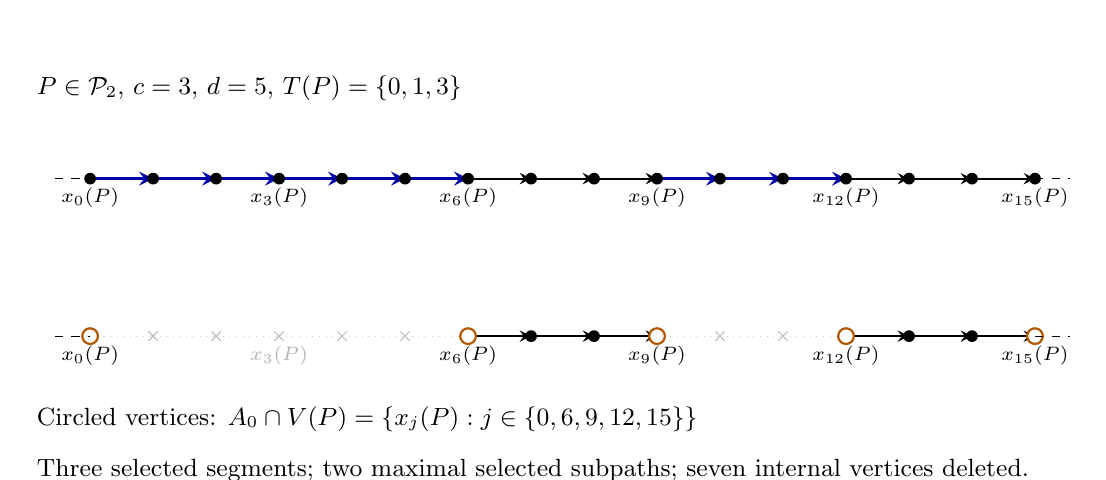
\begin{tikzpicture}[x=1cm,y=1cm,font=\small,>=stealth,
 dot/.style={circle,fill=black,inner sep=1.5pt},
 first/.style={blue!65!black,thick},
 second/.style={red!70!black,thick,dashed},
 shared/.style={green!35!black,very thick},
 spoke/.style={black!45,thin},
 tag/.style={fill=white,inner sep=1pt,font=\scriptsize}]
\node[anchor=west] at (-.8,1.15) {$P\in\mathcal P_2$, $c=3$, $d=5$, $T(P)=\{0,1,3\}$};
\draw[first,very thick,->] (0.0,0)--(0.8,0);
\draw[first,very thick,->] (0.8,0)--(1.6,0);
\draw[first,very thick,->] (1.6,0)--(2.4000000000000004,0);
\draw[first,very thick,->] (2.4000000000000004,0)--(3.2,0);
\draw[first,very thick,->] (3.2,0)--(4.0,0);
\draw[first,very thick,->] (4.0,0)--(4.800000000000001,0);
\draw[black,thick,->] (4.800000000000001,0)--(5.6000000000000005,0);
\draw[black,thick,->] (5.6000000000000005,0)--(6.4,0);
\draw[black,thick,->] (6.4,0)--(7.2,0);
\draw[first,very thick,->] (7.2,0)--(8.0,0);
\draw[first,very thick,->] (8.0,0)--(8.8,0);
\draw[first,very thick,->] (8.8,0)--(9.600000000000001,0);
\draw[black,thick,->] (9.600000000000001,0)--(10.4,0);
\draw[black,thick,->] (10.4,0)--(11.200000000000001,0);
\draw[black,thick,->] (11.200000000000001,0)--(12.0,0);
\node[dot] at (0.0,0) {};
\node[below,black,font=\scriptsize] at (0.0,0) {$x_{0}(P)$};
\node[dot] at (0.8,0) {};
\node[dot] at (1.6,0) {};
\node[dot] at (2.4000000000000004,0) {};
\node[below,black,font=\scriptsize] at (2.4000000000000004,0) {$x_{3}(P)$};
\node[dot] at (3.2,0) {};
\node[dot] at (4.0,0) {};
\node[dot] at (4.800000000000001,0) {};
\node[below,black,font=\scriptsize] at (4.800000000000001,0) {$x_{6}(P)$};
\node[dot] at (5.6000000000000005,0) {};
\node[dot] at (6.4,0) {};
\node[dot] at (7.2,0) {};
\node[below,black,font=\scriptsize] at (7.2,0) {$x_{9}(P)$};
\node[dot] at (8.0,0) {};
\node[dot] at (8.8,0) {};
\node[dot] at (9.600000000000001,0) {};
\node[below,black,font=\scriptsize] at (9.600000000000001,0) {$x_{12}(P)$};
\node[dot] at (10.4,0) {};
\node[dot] at (11.200000000000001,0) {};
\node[dot] at (12.0,0) {};
\node[below,black,font=\scriptsize] at (12.0,0) {$x_{15}(P)$};
\draw[dashed] (-.45,0)--(0,0);\draw[dashed] (12,0)--(12.45,0);
\draw[black!20,dotted] (0.0,-2)--(0.8,-2);
\draw[black!20,dotted] (0.8,-2)--(1.6,-2);
\draw[black!20,dotted] (1.6,-2)--(2.4000000000000004,-2);
\draw[black!20,dotted] (2.4000000000000004,-2)--(3.2,-2);
\draw[black!20,dotted] (3.2,-2)--(4.0,-2);
\draw[black!20,dotted] (4.0,-2)--(4.800000000000001,-2);
\draw[black,thick,->] (4.800000000000001,-2)--(5.6000000000000005,-2);
\draw[black,thick,->] (5.6000000000000005,-2)--(6.4,-2);
\draw[black,thick,->] (6.4,-2)--(7.2,-2);
\draw[black!20,dotted] (7.2,-2)--(8.0,-2);
\draw[black!20,dotted] (8.0,-2)--(8.8,-2);
\draw[black!20,dotted] (8.8,-2)--(9.600000000000001,-2);
\draw[black,thick,->] (9.600000000000001,-2)--(10.4,-2);
\draw[black,thick,->] (10.4,-2)--(11.200000000000001,-2);
\draw[black,thick,->] (11.200000000000001,-2)--(12.0,-2);
\node[circle,draw=orange!70!black,fill=white,thick,inner sep=2pt] at (0.0,-2) {};
\node[below,black,font=\scriptsize] at (0.0,-2) {$x_{0}(P)$};
\draw[black!25] (0.74,-2.06)--(0.8600000000000001,-1.94) (0.74,-1.94)--(0.8600000000000001,-2.06);
\draw[black!25] (1.54,-2.06)--(1.6600000000000001,-1.94) (1.54,-1.94)--(1.6600000000000001,-2.06);
\draw[black!25] (2.3400000000000003,-2.06)--(2.4600000000000004,-1.94) (2.3400000000000003,-1.94)--(2.4600000000000004,-2.06);
\node[below,black!30,font=\scriptsize] at (2.4000000000000004,-2) {$x_{3}(P)$};
\draw[black!25] (3.14,-2.06)--(3.2600000000000002,-1.94) (3.14,-1.94)--(3.2600000000000002,-2.06);
\draw[black!25] (3.94,-2.06)--(4.06,-1.94) (3.94,-1.94)--(4.06,-2.06);
\node[circle,draw=orange!70!black,fill=white,thick,inner sep=2pt] at (4.800000000000001,-2) {};
\node[below,black,font=\scriptsize] at (4.800000000000001,-2) {$x_{6}(P)$};
\node[dot] at (5.6000000000000005,-2) {};
\node[dot] at (6.4,-2) {};
\node[circle,draw=orange!70!black,fill=white,thick,inner sep=2pt] at (7.2,-2) {};
\node[below,black,font=\scriptsize] at (7.2,-2) {$x_{9}(P)$};
\draw[black!25] (7.94,-2.06)--(8.06,-1.94) (7.94,-1.94)--(8.06,-2.06);
\draw[black!25] (8.74,-2.06)--(8.860000000000001,-1.94) (8.74,-1.94)--(8.860000000000001,-2.06);
\node[circle,draw=orange!70!black,fill=white,thick,inner sep=2pt] at (9.600000000000001,-2) {};
\node[below,black,font=\scriptsize] at (9.600000000000001,-2) {$x_{12}(P)$};
\node[dot] at (10.4,-2) {};
\node[dot] at (11.200000000000001,-2) {};
\node[circle,draw=orange!70!black,fill=white,thick,inner sep=2pt] at (12.0,-2) {};
\node[below,black,font=\scriptsize] at (12.0,-2) {$x_{15}(P)$};
\draw[dashed] (-.45,-2)--(0,-2);\draw[dashed] (12,-2)--(12.45,-2);

\node[anchor=west] at (-.8,-3.05)
 {Circled vertices: $A_0\cap V(P)=\{x_j(P):j\in\{0,6,9,12,15\}\}$};
\node[anchor=west] at (-.8,-3.7)
 {Three selected segments; two maximal selected subpaths; seven internal vertices deleted.};

\end{tikzpicture}
\caption{Deleting selected segments of a directed path.
The blue segments form two maximal selected subpaths, whose edges and
internal vertices are deleted in the lower row.
The junction $x_3(P)$ is deleted, whereas the circled vertices form
$A_0\cap V(P)$. Dashed continuations lie outside $P$.}
\label{fig:reconstruction:residual-domains}
\end{figure}


\begin{lemma}
\label{lem:images:residual-structure}
Let $Q,A_0$ be given by \eqref{eq:images:residual-domains}. Let
\begin{equation*}
 m_i:=|\mathcal P_i|\quad(i=1,2),\qquad
 q:=\sum_{P\in\mathcal P_2}|T(P)|,\qquad
 h:=|\mathcal R^{\rm sel}|,\qquad b^{\rm miss}:=dm_2-q,
\end{equation*}
and let $N^{\rm full}:=|V(F)|-|V(\textstyle\bigcup\mathcal D)|-(cd-1)(m_1+m_2)$
be the number of remaining vertices if every segment of every path
in $\mathcal P_2$ were selected. Then $A_0$ is independent in $Q$,
and every component of $Q$ is a
directed path, an isolated vertex or a directed cycle of length at least three.
Moreover,
\begin{equation}
\begin{aligned}
 |V(Q)|&=|V(F)|-|V(\textstyle\bigcup\mathcal D)|-(cd-1)m_1-cq+h,\\
 |A_0|&=2m_1+m_2+b^{\rm miss}+h,\\
 e(Q)&=|V(Q)|-(m_1+h)=|V(Q)|-|\mathcal P^{\rm del}| \ge |V(Q)|-|A_0|,
\end{aligned}
\label{eq:images:remainder-counts}
\end{equation}
\begin{equation}
 |h-m_2|\le b^{\rm miss},\qquad
 |A_0|\le2(m_1+m_2)+2b^{\rm miss},
 \label{eq:images:partial-count-bounds}
\end{equation}
and
\begin{equation}
 (c-1)b^{\rm miss}\le |V(Q)|-N^{\rm full}
 =cb^{\rm miss}+h-m_2\le(c+1)b^{\rm miss}.
 \label{eq:images:full-selection-comparison}
\end{equation}
\end{lemma}
\begin{proof}
Removing a component deletes equally many vertices and edges.
The selected subpaths have $cq$ edges and $cq-h$ internal vertices.
All deleted paths are vertex-disjoint, giving the first and third
equalities in \eqref{eq:images:remainder-counts}.
A path with $q_P$ selected segments in $h_P$ maximal selected subpaths loses $q_P-h_P$
of its $d+1$ vertices $x_{cj}(P)$, leaving $1+(d-q_P)+h_P$ of them.
Together with the two endpoints of each path in $\mathcal P_1$,
this proves the formula for $|A_0|$.

If $q_P>0$, the $h_P$ maximal selected subpaths are separated by
at least $h_P-1$ unselected segments, so $h_P-1\le d-q_P$.
If $q_P=0$, then $h_P=0$ and $1\le d$.
Thus $|h_P-1|\le d-q_P$.
Summing gives $|h-m_2|\le b^{\rm miss}$. Substitution in the two
cardinality formulas proves \eqref{eq:images:partial-count-bounds}
and \eqref{eq:images:full-selection-comparison}.

Distinct vertices $x_{cj}(P)$ on the same path are at least $c\ge3$
edges apart. The disjoint two-edge extensions separate endpoints
of different paths. Thus $A_0$ is independent. Deleting paths from
cycles gives the stated component types. Every deleted path has
two distinct endpoints in $A_0$, so $2(m_1+h)\le|A_0|$, proving
the final edge inequality in \eqref{eq:images:remainder-counts}.
\end{proof}

\paragraph{Prescribed images.}
Let $V,U$ be disjoint finite sets and let $\pi$ be a permutation of $V$.
For each $w\in U$, let $F_w,\mathcal P_{1,w},\mathcal P_{2,w},\mathcal D_w$
satisfy the disjointness and extension conditions above.
Let $\theta_{i,w}:\mathcal P_{i,w}\to\mathcal I_{i,w}$ be bijections to
length-$d$ intervals. Let $a_0(I)$ be the first label of $I$, and let
$a_j(I):=\pi^j(a_0(I))$ and $I^+:=a_d(I)$.
Suppose that $a_0(I),\ldots,a_d(I)$ are distinct for every interval
$I$ and that, for each $w\in U$, the sets $I\cup\{I^+\}$ with
$I\in\mathcal I_{1,w}\mathbin{\dot\cup}\mathcal I_{2,w}$ are pairwise disjoint.
For $I\in\mathcal I_{2,w}$, let $T_{w,I}\subseteq\{0,\ldots,d-1\}$ be fixed.
In \eqref{eq:images:residual-domains}, let $T(P):=T_{w,\theta_{2,w}(P)}$.
The prescribed images on $A_{0,w}$ are
\begin{equation*}
\begin{aligned}
 \phi_w(x_0(P))&:=a_0(\theta_{1,w}(P)),&
 \phi_w(x_{cd}(P))&:=\theta_{1,w}(P)^+
 &&(P\in\mathcal P_{1,w}),\\
 \phi_w(x_{cj}(P))&:=a_j(\theta_{2,w}(P))
 &&&&(P\in\mathcal P_{2,w},\ x_{cj}(P)\in A_{0,w}).
\end{aligned}
\end{equation*}
Let
\begin{equation*}
 E_w^{\rm end}:=\{a_0(I),I^+:I\in\mathcal I_{1,w}\cup\mathcal I_{2,w}\},\qquad
 B_w^{\rm miss}:=\bigcup_{I\in\mathcal I_{2,w}}
                    \{a_j(I):j\notin T_{w,I},\ 0\le j<d\}.
\end{equation*}
For a packing $\mathcal P_w$ of unmarked and marked wheels at hub
$w$, with pairwise disjoint physical edge sets, let
$S_w^j$ be the set of vertices $v$ for which a wheel of $\mathcal P_w$
uses the spoke $(vw,j)$, for $j\in\{0,K\}$.
The $c-1$ unmarked spokes of each marked wheel contribute their
rim endpoints to $S_w^0$.
For $x\in S_w^K$, let $R_{w,x}$ be the directed physical rim walk of
the unique wheel using $xw$. This walk has length $c$ and runs from
$x$ to $\pi(x)$. For an unmarked wheel $W$, we write $C_W$ for its
directed rim.

\begin{lemma}
\label{lem:images:residual-prescriptions}
With the path and interval assignments above, let
$\mathcal P_w=\mathcal P_w^K\dot\cup\mathcal P_w^0$ be, for each
$w\in U$, a packing of marked $c$-wheels and unmarked wheels with
directed rims at $w$, whose physical edge sets are pairwise disjoint.
Suppose
\begin{equation*}
 S_w^K=\bigcup_{I\in\mathcal I_{2,w}}\{a_j(I):j\in T_{w,I}\},\qquad
 S_w^0\cap\bigcup_{I\in\mathcal I_{1,w}\cup\mathcal I_{2,w}}
                    (I\cup\{I^+\})=\varnothing.
\end{equation*}
Let $\kappa_w:\mathcal P_w^0\to\operatorname{Comp}(F_w)$
be injective and length-preserving, with
$\operatorname{im}(\kappa_w)\subseteq\mathcal D_w$.
We define $Q_w,A_{0,w}$ by
\eqref{eq:images:residual-domains} and let
\begin{equation*}
X_w:=A_{0,w}\cup\bigcup_{R\in\mathcal R_w^{\rm sel}}V(R)
                 \cup V\left(\bigcup\operatorname{im}(\kappa_w)\right).
\end{equation*}
There is an injection $\Psi_w:X_w\to V$ extending $\phi_w$, mapping
each selected segment with index $j$ in $P:=\theta_{2,w}^{-1}(I)$
in order onto $R_{w,a_j(I)}$, and mapping $\kappa_w(W)$ in cyclic order
onto $C_W$ for each unmarked wheel $W$. Moreover,
\begin{equation}
 X_w\cap V(Q_w)=A_{0,w},\qquad
 \bigcup_{I\in\mathcal I_{2,w}}(I\cup\{I^+\})\subseteq\Psi_w(X_w),
 \label{eq:images:occupied-intervals}
\end{equation}
and $\phi_w(A_{0,w})\subseteq E_w^{\rm end}\cup B_w^{\rm miss}\cup\pi(B_w^{\rm miss})$.
\end{lemma}
\begin{proof}
Write the physical rim of the wheel using $a_j(I)w$ as $(a_j(I),z_{j,1},\ldots,z_{j,c-1},a_{j+1}(I))$. The
internal labels have unmarked spokes. Within the packing at $w$,
these labels are distinct across all wheels and avoid all extended
intervals. The same holds for the rim labels of unmarked wheels.
Each selected segment is mapped onto this path in order.
If two selected segments are consecutive, both maps send their common
endpoint $x_{c(j+1)}(P)$ to $a_{j+1}(I)$. There are no other repeated labels, by
extended-interval disjointness and the unmarked-spoke exclusion.
Thus each maximal selected subpath maps to a simple path, and distinct such subpaths
and assigned cycle components have disjoint images.

For each assigned cycle component, choose an isomorphism onto its
unmarked wheel rim in cyclic order. Together with these isomorphisms
and $\phi_w$, the segment embeddings define $\Psi_w$: their maps
agree at common junctions, and the remaining prescribed interval
labels avoid all other images. Thus $\Psi_w$ is injective.
No interior of a path in $\mathcal P_{1,w}$ is embedded.

By the definitions of $Q_w$ and $X_w$, the vertices of $X_w$ outside
$V(Q_w)$ are precisely the interiors of the maximal selected
subpaths and the vertices of the assigned cycle components.
Thus $X_w\cap V(Q_w)=A_{0,w}$, proving the first equality in
\eqref{eq:images:occupied-intervals}. For each $P\in\mathcal P_{2,w}$,
every vertex $x_{cj}(P)$ is either internal to a selected subpath or
belongs to $A_{0,w}$. In both cases its image is $a_j(I)$, proving
the inclusion there. For $0<j<d$, the vertex $x_{cj}(P)$ remains in
$A_{0,w}$ precisely when $j-1\notin T(P)$ or $j\notin T(P)$. Its image belongs to $B_w^{\rm miss}$ if segment $j$ is missing,
and to $\pi(B_w^{\rm miss})$ if segment $j-1$ is missing.
The original endpoints lie in $E_w^{\rm end}$, proving the last assertion.
\end{proof}

Consequently, for every $v\in V$,
\begin{equation}
 |\{w:v\in\phi_w(A_{0,w})\}| \le |\{w:v\in E_w^{\rm end}\}|+|\{w:v\in B_w^{\rm miss}\}|+|\{w:\pi^{-1}(v)\in B_w^{\rm miss}\}|.
\label{eq:images:multiplicity}
\end{equation}


\section{Balanced orientations and exact marked indegrees}

The two lemmas in this section perform different operations.
Lemma~\ref{lem:simp:orientation-routing} balances an orientation by
reversing directed paths of length two while avoiding a forbidden graph.
Lemma~\ref{lem:new:marked-indegree-correction} leaves all directions
unchanged and corrects marked indegrees by changing types only on
the specified arcs. For related degree balancing in random graph
partitions, see \cite[Lemma~9.1]{KeevashStaden2022}.

\begin{lemma}
\label{lem:simp:orientation-routing}
Let $n,L$ be positive integers, and let $a,f\ge0$ and $\beta>0$.

Let $G$ be a simple graph on $V$, $|V|=n$, in which every
vertex has even degree. Let $D_0$ be an orientation of $G$
satisfying $d_{D_0}^+(v)=d_G(v)/2\pm a$ for every $v\in V$.
Let $E_{\rm el}\subseteq E(G)$ and let $F$ be a graph on $V$
with $\Delta(F)\le f$.

Suppose that, for all distinct $x,y\in V$,
\begin{equation*}
 |\{z:x\to z\to y\text{ in }D_0,\ xz,zy\in E_{\rm el}\}|
 \ge\beta n,
\end{equation*}
and
\begin{equation}
 \beta n>na/L+2a+4L+2f.
 \label{eq:simp:orientation-routing}
\end{equation}

Then there is a balanced orientation $D$ of $G$, with
$d_D^+(v)=d_D^-(v)=d_G(v)/2$ for every $v\in V$.
The graph $J$ of edges on which $D,D_0$
differ satisfies $E(J)\subseteq E_{\rm el}\setminus E(F)$ and $\Delta(J)\le a+2L$. \end{lemma}
\begin{proof}
Let $D'$ denote the current orientation, initially $D_0$.
The integer discrepancies $d_{D'}^+(v)-d_G(v)/2$ sum to zero.
If $d_{D'}^+(x)>d_G(x)/2$ and $d_{D'}^+(y)<d_G(y)/2$, we reverse a directed
path $x\to z\to y$ whose edges belong to $E_{\rm el}\setminus E(F)$
and have not previously been reversed. This reduces the total
positive discrepancy by one and leaves the discrepancy at $z$ unchanged. At most $na$ steps are needed, and each vertex is an endpoint at most
$a$ times. A vertex is excluded as a middle vertex after it has been
used in that role $L$ times. Hence at most $na/L$ vertices reach this
limit. Previously changed edges at $x,y$
exclude at most $2a+4L$ choices for $z$, and $F$
excludes at most $2f$. Equation~\eqref{eq:simp:orientation-routing}
leaves a path $x\to z\to y$ of $D_0$ with both edges in
$E_{\rm el}\setminus E(F)$ and neither previously reversed.
It is therefore also a directed path of $D'$. The procedure ends with every discrepancy
zero, and each vertex meets at most $a+2L$ reversed edges.
\end{proof}


\begin{lemma}
\label{lem:new:marked-indegree-correction}
Let $n\ge1$ be an integer, let $\rho>0$, and let
$0<\eta\le\min\{1,\rho\}$.
Let $P$ be an oriented graph on $n$ vertices, let
$M_0\subseteq E(P)$, let $A\subseteq E(P)$, and let
$f:V(P)\to\mathbb Z_{\ge0}$. Suppose that, for every $v\in V(P)$,
\begin{equation*}
 d_{M_0}^-(v)=f(v)\pm \eta n,\qquad
 d_{A\cap M_0}^-(v)\ge\rho n,\qquad
 d_{A\setminus M_0}^-(v)\ge\rho n.
\end{equation*}
Then there is $M\subseteq E(P)$ such that $d_M^-(v)=f(v)$ for all $v\in V(P)$ and $M\triangle M_0\subseteq A$. Let
$J:=(V(P),\{\{u,v\}:u\to v\in M\triangle M_0\})$. Then
\begin{equation}
 \Delta(J)\le(1+2/\rho)\eta n+n^{3/5}.
 \label{eq:new:orientation-and-types:O2}
\end{equation}
\end{lemma}
The proof is given in Appendix~\ref{app:proof:lem-new-marked-indegree-correction}.


\section{Embedding a small remainder with prescribed vertex images}

Lemma~\ref{lem:new:prescribed-embedding} extends prescribed vertex images to
embeddings of small unions of directed paths, isolated vertices and
cycles. Neighborhood conditions on the sets of permitted images
ensure that the embeddings can be completed, while bounds on the
number of prescribed and newly chosen images control the total
edge use at each vertex.
All paths and cycles in this section are directed. An oriented
graph has no loops and has at most one of the arcs $xy,yx$ for
each pair of distinct vertices.

\begin{definition}[Extending lists]\label{gls:extending-lists}
\label{def:lists:extending}
Let $D$ be an oriented graph on $V$, $|V|=n$, and let $\lambda\ge0$.
A set $L\subseteq V$ is \emph{$\lambda$-extending in $D$} if $|L| \geq \lambda n$ and
\begin{align*}
 |N_D^+(x)\cap L|,\ |N_D^-(x)\cap L|\ge\lambda n \quad(x\in V),\qquad |N_D^+(x)\cap N_D^-(y)\cap L|\ge\lambda n \quad(x\ne y\in V).
\end{align*}
\end{definition}

\begin{lemma}
\label{lem:lists:deletion-bound}
Let $n\ge1$ and $\beta,z,t\ge0$. Let $D_0,D_1$ be oriented graphs
on the same $n$-vertex set $V$, and let $O,L\subseteq V$.
Suppose that $O$ is $\beta$-extending in
$D_0$, $|O\setminus L|\le z$, and
$|N_{D_0}^{\pm}(v)\setminus N_{D_1}^{\pm}(v)|\le t$ for every $v\in V$.
Let $\beta':=\beta-(z+2t)/n$. If $\beta'\ge0$, then $L$ is
$\beta'$-extending in $D_1$.
\end{lemma}
\begin{proof}
For distinct $x,y\in V$, we have $|L\cap N_{D_1}^+(x)\cap N_{D_1}^-(y)| \ge |O\cap N_{D_0}^+(x)\cap N_{D_0}^-(y)|-z-2t \ge\beta n-z-2t$.
The sets $L\cap N_{D_1}^{+}(x)$ and $L\cap N_{D_1}^{-}(x)$ each
have size at least $\beta n-z-t$, and $|L|\ge\beta n-z$.
Thus $L$ is $\beta'$-extending.
\end{proof}

\begin{lemma}[Embedding with prescribed images]
\label{lem:new:prescribed-embedding}
Let $0<\beta\le1$, $0<\delta\le(\beta/100)^2$ and
$n\ge\max\{100/\beta,2/\sqrt\delta\}$.
Let $D\subseteq D^*$ be oriented graphs on a set $V$ of size $n$,
and let $W$ be a set with $|W|\le n$.
For each $w\in W$, let $L_w\subseteq V$ be $\beta$-extending in $D$.
For each $w\in W$, let $Q_w$ be a vertex-disjoint union of directed
paths, isolated vertices and directed cycles of length at least three,
with $|V(Q_w)|\le\delta n$. Let $A_w\subseteq V(Q_w)$ and let
$\phi_w:A_w\to V$ be an embedding of $Q_w[A_w]$ in $D^*$.
Let $E_w^0:=E(\phi_w(Q_w[A_w]))$ and assume
\begin{equation*}
    E_{\rm phys}((V,E_w^0))\cap E_{\rm phys}((V,E_{w'}^0))=\varnothing\quad(w\ne w'\in W),\qquad |\{w\in W:v\in\phi_w(A_w)\}|\le\delta n\quad(v\in V).
\end{equation*}

Let $J$ be a graph on $V$ with $\Delta(J)\le\delta n$, where the set $E(J)$ and the sets $E_{\rm phys}((V,E_w^0))$ are not necessarily disjoint.
Then there exist embeddings $\Phi_w:Q_w\to D^*$, $w\in W$,
with the following properties. Writing
$E_w:=E(\Phi_w(Q_w))$ and $F:=(V,\bigcup_{w\in W}E_{\rm phys}((V,E_w)))$, we have
\begin{enumerate}[label=\textup{(\roman*)}]
    \item For every $w\in W$,
    \begin{equation*}
        \Phi_w|_{A_w}=\phi_w,\qquad
        \Phi_w(V(Q_w)\setminus A_w)\subseteq L_w,\qquad
        E_w\setminus E_w^0\subseteq E(D).
    \end{equation*}
    \item The edge images satisfy
    \begin{equation*}
        E_{\rm phys}((V,E_w))\cap E_{\rm phys}((V,E_{w'}))=\varnothing\quad(w\ne w'\in W),\qquad
        E_{\rm phys}((V,E_w\setminus E_w^0))\cap E(J)=\varnothing\quad(w\in W).
    \end{equation*}
    \item The union and the new vertex images satisfy $\Delta(F)\le5\sqrt\delta\,n$, \begin{equation*}
        |\{(w,x):w\in W,\ x\in V(Q_w)\setminus A_w,\ \Phi_w(x)=v\}| \le\sqrt\delta\,n+1\quad(v\in V).
    \end{equation*}
\end{enumerate}
\end{lemma}

\begin{proof}
We use the greedy embedding argument of
Keevash and Staden~\cite[Section~9.2]{KeevashStaden2022},
reserving all prescribed edges before choosing any free image.
Put $t:=\sqrt\delta\,n$. At each stage, let $f(v)$ be the number of
already embedded vertices in the sets $V(Q_w)\setminus A_w$, summed
over $w\in W$, whose image is $v$. A vertex $v$ is excluded as a new
free image whenever $f(v)\ge t$. At every stage at most $t$ labels are
excluded for this reason, since at most $\delta n^2$ free vertices
are embedded in total. Thus every final $f(v)$ is at most $t+1$.

Let $F_{\rm used}$ be the graph on $V$ whose edges are all prescribed
physical edges, including those assigned to indices not yet processed, and all
new physical edges already embedded. Each prescribed occurrence
contributes at most two incident edges, as does each free occurrence.
Hence $\Delta(F_{\rm used})\le2\delta n+2t+2$ and
$\Delta(J\cup F_{\rm used})\le3\delta n+2t+2\le8t$, since $t\ge2$
and $\delta\le1$. When embedding $Q_w$, its prescribed and previously chosen
images exclude at most $\delta n$ vertices. If the predecessor and
successor of an unembedded position have distinct images $x,y$,
the number of available images for that position is at least
$\beta n-t-\delta n-16t>0$, using $\sqrt\delta\le\beta/100$.
A choice requiring just one incident arc has the same bound with
$16t$ replaced by $8t$. A choice requiring no arc need only avoid
the images already used or prescribed at $w$ and the vertices
with $f(v)\ge t$. Every new physical edge avoids $J\cup F_{\rm used}$.

We process the components of $Q_w-A_w$. A component that is not
a whole cycle is a path, possibly a single vertex, with at most
one prescribed predecessor and one prescribed successor.
When both prescribed vertices are present and distinct, we embed
forward until only one free vertex remains. If its predecessor and
successor have images $x,y$, we choose its image
\begin{equation*}
 z\in L_w\cap N_D^+(x)\cap N_D^-(y),\qquad f(z)<t,
 \qquad \{x,z\},\{z,y\}\notin E(J)\cup E(F_{\rm used}),
\end{equation*}
avoiding the prescribed and previously chosen images at $w$.
The images $x,y$ are distinct by injectivity.
If the prescribed predecessor and successor are the same vertex
$a\in A_w$, the component lies in a cycle with exactly one vertex
of $A_w$. Since this cycle has length at least three, it has at
least two free vertices. We first embed the successor of $a$ in
$L_w\cap N_D^+(\phi_w(a))$, subject to the same exclusions.
Its image differs from $\phi_w(a)$, so we can embed forward and
use the two-neighbor choice for the last free vertex.
A path with only a prescribed predecessor is embedded forward,
and one with only a prescribed successor is embedded backward.
If neither is present, its first image is chosen freely in $L_w$.
For a whole cycle, we choose the first image freely in $L_w$,
embed forward, and use the two-neighbor choice for its last vertex.
The two boundary images are distinct because the cycle has length
at least three and the partial embedding is injective.
Components wholly contained in $A_w$ have already been embedded.
Every needed choice thus exists by the preceding estimates.

The construction extends every prescribed map, uses $L_w$ for
all free images and $D$ for all new arcs, and preserves injectivity
and physical edge-disjointness. Every new edge avoids $J$, whereas
the prescribed edges are allowed to belong to $J$. Finally
$\Delta(F)\le2\delta n+2t+2\le5\sqrt\delta\,n$ and $f(v)\le\sqrt\delta\,n+1$, which are the remaining
conclusions.
\end{proof}

For an oriented matching $M$, we write $\partial M$ for its endpoint
set and $e(M):=|E(M)|$. Closed neighborhoods in the next proof are
taken in the underlying undirected graph.

\begin{lemma}
\label{lem:new:prescribed-positions}
Let $Q$ be a finite directed graph whose components are directed
paths, isolated vertices, and directed cycles of length at least three.
Let $A_0\subseteq V(Q)$ be independent. Let $X$ be a finite set
and let $\psi:A_0\to X$ be injective.
Let $M$ be an oriented matching on $X$ and let $Z\subseteq X$.
Assume that $\psi(A_0)$, $\partial M$ and $Z$ are pairwise disjoint
and that $e(Q)\ge|V(Q)|-|A_0|$. If
\begin{equation}
 |V(Q)|\ge8|A_0|+8e(M)+4|Z|+10,
 \tag{S6}\label{eq:new:late:S6}
\end{equation}
then there are $A_0\subseteq A\subseteq V(Q)$ and an injection
$\psi':A\to X$ extending $\psi$ such that $\psi'(A)=\psi(A_0)\mathbin{\dot\cup}\partial M \mathbin{\dot\cup}Z$ and $E(\psi'(Q[A]))=E(M)$.
Here, the edge image is the oriented arc set $\{\psi'(x)\to\psi'(y):x\to y\in E(Q[A])\}$.
\end{lemma}
\begin{proof}
Put $a_0:=|A_0|$, $m:=e(M)$ and $z:=|Z|$.
We first delete
$A_0\cup\bigcup_{x\in A_0}(N_Q^+(x)\cup N_Q^-(x))$ from $Q$.
The deleted set has at most
$3a_0$ vertices and meets at most $6a_0$ edges. Since
$e(Q)\ge|V(Q)|-a_0$, this graph has at least $|V(Q)|-7a_0$ edges.
We choose $m$ edges successively, removing the closed neighborhood
of their endpoints after each choice. Each step removes at most
four vertices and eight edges. When $m>0$, before its last choice
at least $|V(Q)|-7a_0-8(m-1)>0$ edges remain by
\eqref{eq:new:late:S6}.

We then choose $z$ further vertices successively, removing the
closed neighborhood of each chosen vertex. When $z>0$, before its last choice at least
$|V(Q)|-3a_0-4m-3(z-1)>0$ vertices remain.
The selected edges form an induced matching, avoid $A_0$ and all
its neighbors, and have no adjacency to the selected single vertices.
The latter vertices are mutually nonadjacent and avoid $A_0$ and
its neighbors. Thus the only arcs induced by the union of $A_0$
and all selected positions are the selected matching edges.
We map the selected edges bijectively onto $M$, respecting their
orientations, and the selected single vertices bijectively onto $Z$.
The image sets are disjoint, so these maps together with $\psi$
give the required injection.
\end{proof}



\begin{lemma}\label{lem:new:prescribed-edge-assignment}
Let $n\ge1$ be an integer, let $a>0$ and $0\le b\le a/16$.
Let $M$ be a simple graph on $V$, $|V|=n$, and let $W$ be a set
with $|W|\le n$.
For each edge $e\in E(M)$, let $\mathcal L(e)\subseteq W$
have size at least $an$.
For each vertex $v$, let $\mathcal B(v)\subseteq W$ be a set
of forbidden indices, of size at most $bn$.
Assume $\Delta(M)\le bn$.
Let $K:=\left\lceil\frac{4|E(M)|}{an}\right\rceil$. Then there is an assignment $f:E(M)\to W$ such that
\begin{enumerate}[label=\textup{(\roman*)}]
    \item $f(uv)\in\mathcal L(uv)\setminus (\mathcal B(u)\cup\mathcal B(v))$;
    \item $f^{-1}(w)$ is a matching for every $w\in W$;
    \item $|f^{-1}(w)|\le K$ for every $w\in W$.
\end{enumerate}
\end{lemma}

\begin{proof}
If $E(M)=\varnothing$, take the empty assignment. Hence assume
$E(M)\ne\varnothing$, so $K\ge1$.

Process the edges in any order. For an edge $uv$, the two
forbidden sets exclude at most $2bn$ indices. Earlier edges at
$u$ or $v$ exclude at most $2bn$ further indices.
The number of indices already assigned $K$ edges is at most
$|E(M)|/K\le an/4$. Thus fewer than $4bn+an/4\le an/2$ indices in its list are excluded. We choose any remaining one.
This preserves all three requirements at every step.
\end{proof}


\paragraph{Neighborhood lists in a raw interval sample.}
Let $G$ be a graph on $V$, let $W$ be disjoint from $V$, let
$X\subseteq V$, and let $\pi$ be a permutation of $V$ with $L_\pi>10d$,
where $d\ge2$ is an integer. Let $q:W\to[0,1/8]$, $s:W\to[0,1]$
and $p\in[0,1/2]$ with $s(w)\le1-(1+1/d)q(w)$.
Let $(\mathcal X_w^g)_{w\in W,g\in\{1,2\}}$ and $(B_{w,x})$ be
a raw interval sample with $\Gamma=\{1,2\}$, $\Sigma=\{0\}$,
$q_1=0$, $q_2=q$ and $s_0=s$, as in
Definition~\ref{def:four:local-interval-law}.
Independently of this sample, let $(C_e)_{e\in E(G)}$ be independent
random variables with
\begin{equation*}
 \Pr(C_{\{x,y\}}=(x,y))=\Pr(C_{\{x,y\}}=(y,x))=p,
 \qquad \Pr(C_{\{x,y\}}=\bot)=1-2p.
\end{equation*}
We define the oriented graph $D_0$ by
$E(D_0):=\{x\to y:xy\in E(G),\ C_{xy}=(x,y),\ \operatorname{dist}_\pi(x,y)>3d\}$. Let $H_0$ have edge set
$E(H_0):=\{xw:B_{w,x}=0,\ x\notin \bigcup_{I\in\mathcal X_w^2}(I\cup\{I^+\})\}$, and let
$L_w^0:=N_{H_0}(w)\setminus X$.
For subfamilies $\mathcal Y_w\subseteq\mathcal X_w^2$, let
\begin{equation*}
 \bar H(\mathcal Y):=
 \left(V,W;\left\{xw:B_{w,x}=0,\
 x\notin\bigcup_{I\in\mathcal Y_w}(I\cup\{I^+\})\right\}\right).
\end{equation*}
The graph $H_0$ and every graph $\bar H(\mathcal Y)$ use the same
label variables $B_{w,x}$.

\Needspace{8\baselineskip}
\begin{lemma}
\label{lem:list:raw}
Let $0<\alpha_{\rm list}<1/2$, $0<p_{\rm list}\le1/2$ and
$0<s_{\rm list}\le1$, and let $\beta_{\rm list}:=\alpha_{\rm list}p_{\rm list}^2s_{\rm list}/16$. For every
integer $d\ge2$ there is $n_0\in\mathbb N$, depending only on
these parameters, such
that the following holds for $n\ge n_0$.
Let $G$ be a graph on $V$, where $|V|=n$, let $W$ be disjoint
from $V$ with $|W|\le n$, and let $X\subseteq V$ satisfy
$\delta(G)\ge(1/2+\alpha_{\rm list})n$ and $|X|\le\alpha_{\rm list}n/2$. Let $\pi$ be a permutation of $V$
with $L_\pi>10d$.
Let $q:W\to[0,1/8]$, $s:W\to[s_{\rm list},1]$ and
$p\in[p_{\rm list},1/2]$ with $s(w)\le1-(1+1/d)q(w)$.

In the raw interval experiment above, with probability at least
$1-n^{-10}$,
\begin{equation}
 L_w^0\text{ is }12\beta_{\rm list}\text{-extending in }D_0
 \quad\text{for every }w\in W.
 \label{eq:list:raw-bounds}
\end{equation}
If $|W|\ge\kappa n$ for a fixed $\kappa>0$, then, after allowing
$n_0$ also to depend on $\kappa$, the same event satisfies
\begin{equation}
 |N_{H_0}(x)\cap N_{H_0}(y)|\ge\tfrac12e^{-3}s_{\rm list}^2|W|
 \quad(x\ne y\in V).
 \label{eq:list:common-indices}
\end{equation}
\end{lemma}
The proof is given in Appendix~\ref{app:proof:lem-list-raw}.

\Needspace{8\baselineskip}
\begin{lemma}
\label{lem:new:ordinary-list-extensions}
Let $D_0,H_0,(\mathcal X_w^2)$ be the random graphs and intervals
of Lemma~\ref{lem:list:raw}, with the same parameters, and let
$\bar H(\mathcal Y)$ be defined above for
$\mathcal Y_w\subseteq\mathcal X_w^2$.
Let $\zeta_{\rm list}:=\beta_{\rm list}/10$.
On the event in Lemma~\ref{lem:list:raw}, the following implication
holds simultaneously for every
$\mathcal Y$, every oriented graph $D$ with
$E(D)\subseteq\{x\to y:xy\in E(G),\operatorname{dist}_\pi(x,y)>3d\}$,
every bipartite graph $H$ on $V,W$, and all $Z_w\subseteq V$.
If
\begin{equation*}
 \Delta\bigl((V,E_{\rm phys}(D\triangle D_0))\bigr)\le\zeta_{\rm list}n,
 \quad\Delta(H\triangle\bar H(\mathcal Y))\le\zeta_{\rm list}n,
 \quad |Z_w|\le\zeta_{\rm list}n\quad(w\in W),
\end{equation*}
then every $L_w:=N_H(w)\setminus(X\cup Z_w)$ is
$\beta_{\rm list}$-extending in $D$.
\end{lemma}
\begin{proof}
Fix an outcome satisfying \eqref{eq:list:raw-bounds} and any
$\mathcal Y,D,H,(Z_w)$ satisfying the hypotheses. The shared label
variables and $\mathcal Y_w\subseteq\mathcal X_w^2$ give
$H_0\subseteq\bar H(\mathcal Y)$. Consequently, for
$L_w=N_H(w)\setminus(X\cup Z_w)$,
\begin{equation*}
 L_w^0\setminus L_w\subseteq
 (N_{\bar H(\mathcal Y)}(w)\setminus N_H(w))\cup Z_w,
 \qquad |L_w^0\setminus L_w|\le2\zeta_{\rm list}n.
\end{equation*}
The bound on $\Delta((V,E_{\rm phys}(D\triangle D_0)))$ also gives
$|N_{D_0}^{\pm}(v)\setminus N_D^{\pm}(v)|\le\zeta_{\rm list}n$
for every $v\in V$. Lemma~\ref{lem:lists:deletion-bound}, with
$(O,L,z,t)=(L_w^0,L_w,2\zeta_{\rm list}n,\zeta_{\rm list}n)$,
gives extending coefficient $12\beta_{\rm list}-4\zeta_{\rm list}
\ge\beta_{\rm list}$, simultaneously for all the stated choices.

\end{proof}

\section{Ordinary preparation}\label{sec:family:ordinary-preparation}
\subsection{Candidate wheels shared by the two preparations}
\label{subsec:preparation:shared-candidates}
The matching hypergraphs used here and in
Section~\ref{sec:family:long-preparation} have physical rim edges and
spokes as vertices. Each candidate wheel contributes the set of its
physical rim edges and spokes as a hyperedge. This construction
and the hub-dependent normalization of wheel weights follow the
approach of Keevash and Staden~\cite[Sections~6--7]{KeevashStaden2022}.
Here, the rim weights are supplied by fractional cycle decompositions.
Let $P$ be a graph on $V$, let $U$ be disjoint from $V$, and let
$\pi$ be a permutation of $V$. Let
$E_V:=E(P)$, $E_{VU}:=\{\{v,u\}:v\in V,\ u\in U\}$ and
$E:=E_V\dot\cup E_{VU}$. We identify $V\times U$ with $E_{VU}$.
We recall the candidate wheels and their physical edge sets from
\eqref{eq:mixed:ordered-physical-map}--\eqref{eq:mixed:physical-incidence}.
An unmarked candidate has index $i=(0,w,r,\mathbf x)$ with integer $r\ge3$,
and a marked candidate has index $i=(K,w,c,\mathbf x)$ with integer $c\ge4$.
Here $w\in U$ and $\mathbf x=(x_0,\ldots,x_{q_i-1})$ has distinct
entries in $V$, with $q_i:=r$ or $c$, respectively. We denote the
first entry of $i$ by $\tau_i\in\{0,K\}$. Its physical rim
edges are the consecutive edges $x_hx_{h+1}$ for $0\le h<q_i-1$,
together with $x_{q_i-1}x_0$ in the unmarked case or
$x_{q_i-1}\pi(x_0)$ in the marked case. All these edges are distinct
members of $E(P)$. Writing $E_V(i)$ for their set, let
\begin{equation*}
 E_U(i):=\{\{x_h,w\}:0\le h<q_i\},\qquad
 \iota(i):=E_V(i)\cup E_U(i).
\end{equation*}
Let $\mathcal I$ be a set of these candidate indices.
In an unmarked candidate all auxiliary arcs and spokes have type $0$.
In a marked candidate only the closing arc and the spoke $x_0w$
have type $K$. These types belong to the candidate occurrences.
In ordinary preparation they do not assign a permanent type to a
physical rim edge shared by different candidates.
For each $e\in E$, let $\Sigma_e$ be its finite set of possible sampling states.



\paragraph{Indexed wheel hypergraphs and their weights.}
For\phantomsection\label{gls:indexed-wheel-hypergraph-for-preparation} each candidate $i\in\mathcal I$, let
$s_i\in\prod_{e\in\iota(i)}\Sigma_e$ be fixed required states. Let
$\Sigma_e^{\rm app}\subseteq\Sigma_e$ contain every required state at $e$.
For an assignment $\sigma$, we define an indexed hypergraph by
\begin{equation}
V(\mathcal H(\sigma)):=\{e\in E:\sigma(e)\in\Sigma_e^{\rm app}\},\qquad E(\mathcal H(\sigma)):=\{i\in\mathcal
I:\sigma|_{\iota(i)}=s_i\},\qquad \iota_{\mathcal H(\sigma)}(i):=\iota(i).
\label{eq:preparation:incidence-hypergraph}
\end{equation}
Each $e\in E$ with $\sigma(e)\in\Sigma_e^{\rm app}$ is one vertex,
even if it belongs to no realized candidate.
Distinct candidate indices remain distinct hyperedges even if their
incidence sets agree. Let $J_i(f):=\mathbf1_{\{\sigma(f)=s_i(f)\}}$.

Let\phantomsection\label{gls:indexed-wheel-hypergraph-for-preparation:deleted}\label{gls:preparation-potential-loads-and-hub-totals} $\Omega:\mathcal I\to\mathbb R_{\ge0}$. For $F\subseteq P$, let
$\mathcal H_F$ be obtained from $\mathcal H(\sigma)$ by deleting the
vertices $E(F)\cap V(\mathcal H(\sigma))$ and their incident hyperedges,
and let $\Omega_F:=\Omega|_{E(\mathcal H_F)}$. All spoke vertices and
all other isolated vertices are retained. For $a\in\Sigma_e^{\rm app}$ let
$\mathcal I(e,a):=\{i\in\mathcal I:e\in\iota(i),\ s_i(e)=a\}$. We define
\begin{equation}
 Z^F_{e,a}:=
 \sum_{\substack{i\in\mathcal I(e,a)\\
       (E_V(i)\setminus\{e\})\cap E(F)=\varnothing}}
       \Omega(i)\prod_{f\in\iota(i)\setminus\{e\}}J_i(f).
 \label{eq:preparation:wheel-deletion}
\end{equation}
Each product omits $J_i(e)=\ind_{\{\sigma(e)=a\}}$, even when
$\sigma(e)\ne a$ or $e\in E(F)$.
If $\sigma(e)=a$ and $e\notin E(F)$, then
$Z^F_{e,a}=d_{\Omega_F}^{\mathcal H_F}(e)$.
Let\phantomsection\label{gls:preparation-potential-loads-and-hub-totals:hub-totals} $\mathcal I^0_{r,w}$ be the unmarked $r$-wheel candidates at hub $w$.
The total weight of those realized candidates whose rim edges avoid $E(F)$ is
\begin{equation}
 T^F_{r,w}:=
 \sum_{\substack{i\in\mathcal I^0_{r,w}\\E_V(i)\cap E(F)=\varnothing}}
       \Omega(i)\prod_{f\in\iota(i)}J_i(f).
\end{equation}
We write
\begin{equation}
 Z_{e,a}:=Z^{\varnothing}_{e,a},\qquad T_{r,w}:=T^{\varnothing}_{r,w}.
 \label{eq:preparation:wheel-potential}
\end{equation}

\paragraph{Concentration of weighted wheel sums.}
Suppose $n=|V|\ge1$, $|U|\le n$, and the lengths lie in a fixed
finite set $\mathcal L$. Let $d\ge2$ be an integer. Let $\sigma$
have the law of the approximate-packing rim states and raw pair
states in the \hyperref[step:ordinary:sample]{ordinary sampling experiment}
or the \hyperref[step:long:sample]{long-class sampling experiment}
defined below, with their stated sampling probabilities.
Here $\Sigma_e^{\rm app}$ consists of the approximate-packing states
permitted at $e$ in the chosen experiment. The spoke states are
given by~\eqref{eq:interval:assignment} for the raw interval sample
of Definition~\ref{def:four:local-interval-law}, independently of the
rim-edge states, which are chosen independently for distinct physical edges.
The candidate set $\mathcal I$, the required-state functions $s_i$
and the coefficients $\Omega(i)$ are fixed before sampling. Assume
\begin{equation}
 0\le\Omega(i)\le A_{q_i}n^{1-q_i}\qquad(i\in\mathcal I).
 \label{eq:preparation:shared-coefficient-bound}
\end{equation}
For every $\eta_{\rm app}>0$, there are constants $C_d,c_d>0$,
depending only on $\mathcal L$, $(A_q)_{q\in\mathcal L}$, $d$ and
$\eta_{\rm app}$, such that, with failure probability at most
$C_dn^2\exp(-c_dn)$,
\begin{equation}
 Z_{e,a}=\mathbb EZ_{e,a}\pm \eta_{\rm app}/2,
 \qquad T_{r,w}=\mathbb ET_{r,w}\pm \eta_{\rm app}n/2
\label{eq:preparation:raw-concentration}
\end{equation}
simultaneously for every $e\in E$, $a\in\Sigma_e^{\rm app}$,
$r\in\mathcal L$ and $w\in U$.

\begin{proof}[Proof of \eqref{eq:preparation:raw-concentration}]
In each of the two experiments there are at most four approximate-packing
states at a physical rim edge and at most two at a spoke. The required-state indicators are
$I_{f,b}:=\mathbf1_{\{\sigma(f)=b\}}$. The indicators for the different states of a fixed physical rim edge
$f$ are all functions of the same random variable $\sigma(f)$.
Let $b_Z(f,b)$ and $b_T(f,b)$ be the sums of coefficients of terms
containing $I_{f,b}$ in $Z_{e,a}$ and $T_{r,w}/n$, respectively.
Fixing $t$ distinct tuple positions leaves at most $n^{q_i-t}$
tuples. With $\Omega(i)\le A_{q_i}n^{1-q_i}$, this gives,
for each polynomial separately, the following partition
$\mathscr J_1\dot\cup \mathscr J_2$ of the indicators with positive coefficient sum:
\begin{equation}
\begin{array}{c|cc}
 &\mathscr J_1&\mathscr J_2\\\hline
 Z_{e,a}& |\mathscr J_1|\le Cn,\ b_Z(f,b)\le C/n
         &|\mathscr J_2|\le Cn^2,\ b_Z(f,b)\le C/n^2\\
 T_{r,w}/n& |\mathscr J_1|\le Cn,\ b_T(f,b)\le C/n
         &|\mathscr J_2|\le Cn^2,\ b_T(f,b)\le C/n^2.
\end{array}
\label{eq:preparation:incidence-influences}
\end{equation}
Here, $C$ depends only on the fixed lengths and coefficient bounds.
For a spoke root at $w$, $\mathscr J_1$ consists of the state
indicators for spokes at $w$ and for physical rim edges having
an auxiliary representation that contains the root label.
Spokes at other hubs contribute zero.
For a rim-edge root, $\mathscr J_1$ consists of the state
indicators for physical rim edges sharing a possible auxiliary
endpoint with the root, and for spokes at a possible auxiliary
label of the root. The other indicators with positive coefficient
sum form $\mathscr J_2$.
Fixing one further label, including the hub when needed,
gives the first coefficient bound; fixing two gives the second.
For a rim-edge root $\{x,y\}$,
its possible auxiliary labels belong to
$\{x,y,\pi^{-1}(x),\pi^{-1}(y)\}$.
There are at most two orientations and $q_i$ positions for each
choice of $\tau_i\in\{0,K\}$. Any physical rim edge with a representation meeting
one of these labels is incident with that label or its successor.
There are therefore at most $16n$ such unordered edges, and
only a bounded number of required states for each edge.
For $T_{r,w}/n$, the two sets consist of the indicators for
spokes at $w$ and for physical rim edges, respectively,
restricted to indicators with positive coefficient sum.
The additional factor $1/n$ gives the displayed bounds.

The activation, start color and label color at each $(w,x)$
form one random vector. These vectors are mutually independent. For a fixed hub $w$,
the state of $vw$ depends on the start colors at
$\pi^{-d}(v),\ldots,v$ and on the activation variables within
$d$ steps of each start, hence only on
vectors at $(w,\pi^{-2d}(v)),\ldots,(w,\pi^d(v))$.
Conversely, changing the vector at $(w,x)$ can affect only the
spokes $vw$ with $v\in\{\pi^{-d}(x),\ldots,\pi^{2d}(x)\}$. Thus a raw spoke state depends on at
most $3d+1$ vectors, and one vector changes at most $3d+1$ spoke states.
Each spoke has two approximate state indicators. Changing the state of one physical rim edge
alters at most two rim-state indicators. Thus
$B_d:=2(3d+1)$ bounds both the number of coordinates determining
one indicator and the number of indicators affected by one coordinate. We apply
Lemma~\ref{lem:pr:wi-interactions} with $a=n$, $B=B_d$ and the two
rows of \eqref{eq:preparation:incidence-influences}. In each application, the sum of squared bounded-difference constants is at most $2C^3B_d^3/n$. McDiarmid's bounded-differences inequality
(Theorem~\ref{thm:prelim:bounded-differences}), with deviation
$\eta_{\rm app}/2$ for $Z_{e,a}$ and $T_{r,w}/n$, gives failure
probability at most $2\exp(-c_dn)$ for each sum.
There are $O(n^2)$ pairs $(e,a)$ and $O(n)$ pairs $(r,w)$,
so a union bound proves \eqref{eq:preparation:raw-concentration}
with the stated failure probability.
No conditioning on the root is used: a coordinate affecting a
nonomitted indicator is still counted even if it also determines the root.
\end{proof}

\begin{lemma}
\label{lem:pr:wheel-codegrees-deletion}
Let $\mathcal I$ be a set of the unmarked and marked wheel candidates
defined above, with physical incidence sets $\iota(i)$ and required
states $s_i$.
Suppose $n=|V|\ge1$, $|U|\le n$, the lengths $q_i$ belong to a fixed
finite set $\mathcal L$, and
$0\le\Omega(i)\le A_{q_i}n^{1-q_i}$.
There are constants $C_L,C_T$, depending only on $\mathcal L$ and
$(A_q)_{q\in\mathcal L}$, such that, for every assignment
$\sigma\in\prod_{e\in E}\Sigma_e$, every $u\ge0$ and
$F\subseteq P$ with $\Delta(F)\le un$,
\begin{equation}
0\le Z_{e,a}-Z^F_{e,a}\le C_Lu \quad (e\in E,\ a\in\Sigma_e^{\rm app}),\qquad 0\le T_{r,w}-T^F_{r,w}\le C_Tun
\quad (r\in\mathcal L,\ w\in U).
\label{eq:preparation:common-deletion}
\end{equation}
\end{lemma}
The proof is given in Appendix~\ref{app:proof:lem-pr-wheel-codegrees-deletion}.

\begin{lemma}
\label{lem:preparation:rounding}
Let $R\ge2$, $d,L\ge1$ be integers, let $K>0$, and let
$0<\lambda<\theta/2$ with $\theta\le1/100$. There are $\eta>0$ and $n_0$ such that
the following holds for $n\ge n_0$.
Let $\mathcal H$ have at most $n^3$ vertices and edge sizes between
$2$ and $R$, with nonnegative weights $w$ satisfying
$d_w(v)=1\pm\eta$ and $d_w(u,v)\le K/n$ for $u\ne v$.
Let $\mathcal S\subseteq2^{V(\mathcal H)}$ have at most $n^3$ members,
each of size at most $6n$. Let $\mathcal F$ contain at most $n^3$
functions $g:E(\mathcal H)\to[0,1]$, with numbers
$t_g\ge\theta n/(100L^2)$ satisfying
$W_g=(1-\theta)t_g\pm \lambda t_g/10$, where
$W_g:=\sum_hg(h)w(h)$.
Then there is a matching $M$ such that
\begin{equation*}
 |S\setminus V(M)|\le\lambda n\quad(S\in\mathcal S),\qquad
 |S\setminus V(M)|\le\lambda n/(10d)\quad(S\in\mathcal S,\ |S|\le n),
\end{equation*}
and $g(M)=(1-\theta)t_g\pm \lambda t_g/5$ for every $g\in\mathcal F$.
\end{lemma}
\begin{proof}
Apply Lemma~\ref{lem:new:weighted-resource-matching} with
\begin{equation*}
 (r,B,K,a,\gamma)=
 \bigl(R,3,K,\min\{\lambda/(10d),\theta/(200L^2)\},
                    \min\{1/2,\lambda/(10d),\lambda/10\}\bigr),
\end{equation*}
and let $\eta$ be its tolerance. Sets smaller than $\lambda n/(10d)$
may be omitted. Since $\theta\le1/100$ and $\lambda<\theta/2$,
$W_g\ge t_g/2\ge an$ and $W_g\le t_g$.
The lemma gives $|S\setminus V(M)|\le\gamma|S|$ for each retained
set and
$|g(M)-(1-\theta)t_g|\le\gamma W_g+\lambda t_g/10\le\lambda t_g/5$.
The set bounds follow from $|S|\le6n$ and $\gamma\le\lambda/(10d)$,
including the omitted sets.
\end{proof}

\subsection{Proof of Proposition~\ref{prop:family:ordinary-preparation}}


We reserve equally many $r_*$-cycles in each factor. A common sampling
event supplies an absorber and the estimates used for every later
corrected graph $S$. In each such $S$, we first pack most of the
complements with wheels, then embed their remaining vertices and edges
with prescribed images. The resulting unused edges and spokes satisfy
the exact identities and protection conditions of
Proposition~\ref{prop:completion:ordinary-construction}, which completes
the reserved cycles.

For an $n$-vertex two-factor $F_w$, we write $f_{r,w}:=r\,\#\{\text{components of }F_w\text{ of length }r\}/n$ for all $r \geq 3$.

\begin{proof}[Proof of Proposition~\ref{prop:family:ordinary-preparation}]
\startlocalclaims
The numerical parameters
$\vartheta,\alpha_0,\epsilon_{\max},\varrho_*,\beta,r_*$ are fixed.
Put $s_0:=\beta/100$.
Let $\beta_{\rm raw}$ be the coefficient $\beta_{\rm list}$ in
Lemma~\ref{lem:list:raw} with
$(\alpha_{\rm list},p_{\rm list},s_{\rm list})
=(\min\{\alpha_0,1/4\},\varrho_*s_0/4,s_0/2)$.
We take $a_0>0$ sufficiently small in terms of $s_0,\varrho_*$
and put $a_E:=a_0/2$.
The assumed degree bound is
\begin{equation}\label{eq:family:OH.HP.1}
    D\ge(\vartheta+\alpha_0)n.
\end{equation}
We choose an even auxiliary length
$c\ge\max\{8,c_{\rm succ}(\alpha_0/4)\}$, where $c_{\rm succ}$ is
from Theorem~\ref{thm:four:successor-kernel}.
Since $\vartheta\ge1/2$, equation~\eqref{eq:family:OH.HP.1}
gives its minimum-degree hypothesis with $\beta=\alpha_0/4$.
We fix a sufficiently large constant $C_0=C_0(c)$.
With these constants fixed, we choose an integer cutoff
$L_{\rm cut}\ge r_*$ and auxiliary constants with
\begin{equation*}
\begin{aligned}
\xi\ll\tau\ll\eta_{\rm app}\ll\eta_{\rm match}\ll\lambda
 \ll\frac{1}{L_{\rm cut}}\ll\frac{1}{d}\ll\theta\ll t_{\rm prep}\ll\epsilon \ll\epsilon_{\max},\vartheta,\alpha_0,\varrho_*,\beta,\frac{1}{r_*}, \frac{1}{c},\beta_{\rm raw},a_0,a_E,\frac{1}{C_0}.
\end{aligned}
\end{equation*}
Here, $\eta_{\rm match}$ is the tolerance used in the application of
Lemma~\ref{lem:preparation:rounding} below.
The constants through $\xi$ are fixed before $\chi$, and $1/n\ll\chi,\xi$.

\subsubsection*{Reservation and sampling}
\label{step:ordinary:sample}
Let $M := |U|$, and let $\mathcal S$ be the set of component lengths in the prescribed factors.
\begin{equation*}
    \varrho=2M/D\in[\varrho_*,1], \qquad f_{r_*,w}\ge\beta \quad(w\in U).
\end{equation*}
Put $k_*:=\lfloor s_0n/r_*\rfloor$ and $s:=r_*k_*/n$.
For sufficiently large $n$, $s\in[s_0/2,s_0]$. Fix $k_*$ distinct
$r_*$-components $\mathcal C_w$ of each $F_w$ before sampling.
For a corrected graph $S$, the two degree requirements will be written as
\begin{equation}\label{eq:family:OH.HP.5}
    d_S(v)=2M\quad(v\in V),\qquad \Delta(S\triangle S^0)\le\xi n.
\end{equation}
The sets $I$ and $A$ will be chosen below. The other two requirements are
\begin{equation}\label{eq:family:OH.HP.6}
    S[I]=S^0[I],\qquad A\subseteq E(S).
\end{equation}
For the permutation $\pi$ chosen below, put
$P^{\rm adm}:=P-\{xy\in E(P):\operatorname{dist}_\pi(x,y)\le3d\}$.
We use $\Delta_*$ as in Section~\ref{subsec:pr:representations}.

\paragraph{Component fractions and sampling probabilities.}

We use Proposition~\ref{prop:completion:ordinary-construction} with $(r,s_*,\zeta_{\rm rem})=(r_*,s_0/2,2t_{\rm prep})$ and the present $\epsilon$.
The initial hierarchy implies~\eqref{eq:completion:ordinary-input-hierarchy}, uniformly for $s\in[s_0/2,s_0]$.

After removing the reserved components, define
$f'_{r,w}:=f_{r,w}-s\mathbf1_{\{r=r_*\}}$ and $\ell_w:=\sum_{r>L_{\rm cut}}f'_{r,w}$. Thus $\sum_r
f'_{r,w}=1-s$. Let
$\mathcal R_w:=\{r\le L_{\rm cut}:f'_{r,w}\ge\theta/(100L_{\rm cut})\}$
be the set of short cycle lengths used in the approximate packing at $w$, and put
\begin{equation*}
a_w:=
\begin{cases}
(1-\theta)\ell_w/c,&\ell_w\ge\theta/100,\\
0,&\ell_w<\theta/100,
\end{cases}
\end{equation*}
\begin{equation}
f_{{\rm pack},w}:=(1-\theta)\sum_{r\in\mathcal R_w}f'_{r,w},
\qquad b_w:=(c-1)a_w+f_{{\rm pack},w},
\qquad u_w:=1-s-a_w-b_w.
\end{equation}
Here, $a_w$ and $b_w$ are the marginal probabilities of the
type-$K$ and type-$0$ spokes reserved for approximate packing,
respectively. The ordinary completion graph has no edge types.

The fraction omitted from approximate packing is
$o_w:=\sum_{r\le L_{\rm cut},\ r\notin\mathcal R_w}f'_{r,w}
+\ell_w\mathbf1_{\{\ell_w<\theta/100\}}\le2\theta/100$. Hence
\begin{equation}
u_w=\theta(1-s)+(1-\theta)o_w,
\qquad \theta/2\le u_w\le2\theta.
\label{eq:family:OH.3.5}
\end{equation}
In particular,
\begin{equation}
0\le a_w\le1/c\le1/8,
\qquad b_w=1-s-u_w-a_w\ge1/2
\end{equation}
for the stated choices, uniformly over the prescribed factors.

Fix $\chi$ and choose $L_0$ larger than
the cycle-length bounds for the fixed tuple families. We apply
Proposition~\ref{prop:completion:ordinary-construction} with these values
and the marginal functions $(a_w),(b_w)$ to choose $I,J,\pi$ before exposure.
The initial bound $\epsilon\le\epsilon_{\max}$ gives
$|I|\le\epsilon_{\max}n$.

\paragraph{Choosing the pair states indexed by $U$.}

We use the raw pair assignment in
Definition~\ref{def:ordinary-local-reference} with parameters
$s,d,(a_w),(b_w)$. Its feasibility condition
$s+b_w\le1-(1+1/d)a_w$ is equivalent to $u_w\ge a_w/d$,
which follows from \eqref{eq:family:OH.3.5}, $a_w\le1/c$ and
$1/d\ll\theta$.
Let $O_w:=\{v\in V:\sigma_{\mathcal X}(vw)=\mathrm o_1\}$ and
$B_w^{(2)}:=\{v\in V:\sigma_{\mathcal X}(vw)=\mathrm o_2\}$.
Let $Y_w$ be the union of the color-$2$ intervals and let $E_w^+$
be the set of their terminal successors.
Then
\begin{equation}
 O_w\cap(B_w^{(2)}\cup Y_w\cup E_w^+)=\varnothing,
 \qquad B_w^{(2)}\cap(Y_w\cup E_w^+)=\varnothing.
 \label{eq:family:OH.3.7}
\end{equation}
For every $v\in V$ and $w\in U$, $\Pr(v\in O_w)=s$.
No intervals are removed.

\paragraph{Sampling physical edges of $P$.}

Put
\begin{equation}
p:=\frac1D\sum_{w\in U}(b_w+a_w),
\qquad \bar u:=\frac1M\sum_wu_w.
\end{equation}
Each physical edge of $P$ independently receives one of the following states:

\begin{equation*}
\begin{array}{c|c}
\text{Physical state}&\text{Probability}\\\hline
\text{Completion}&\varrho s\\
\text{Approximate packing}&2p\\
\text{Unassigned in this class}&\varrho\bar u\\
\text{Outside this class}&1-\varrho
\end{array}
\end{equation*}

The probabilities sum to one, since
\begin{equation}
\varrho s+2p+\varrho\bar u=\varrho.
\end{equation}
Independently for each edge and independently of these states,
we choose either orientation with probability $1/2$ and store it for
subsequent use. The probability that a given edge is assigned to approximate packing
with a specified direction is therefore $p$. Let $S^0$ be the spanning graph formed by the edges
assigned to the completion, approximate-packing or unassigned state
of this class. Its edges are retained from $P$ independently with
probability $\varrho$.

The graph $G_1$ consists of the edges assigned to completion in $P^{\rm adm}$,
with their directions forgotten. Independently for each
$e\in E(P^{\rm adm})$, we have $\Pr(e\in E(G_1))=\varrho s$.
The construction of $G_1$ is independent of the pair-state experiment.

As in Section~\ref{subsec:preparation:shared-candidates}, a physical
edge assigned to approximate packing has no assigned type and is one hypergraph vertex in
all its candidate wheels. Equation~\eqref{eq:family:OH.3.5} gives
\begin{equation*}
p=\frac\varrho2(1-s-\bar u)\ge\varrho_*/4.
\end{equation*}
This bound does not depend on $\sum_w a_w$.

The component fractions, sampling probabilities and vortex are fixed
before the edge and pair-state exposure.

\paragraph{Allowed arcs and approximate wheels.}

Ordinary completion uses edges $xy\in E(P)$ with
$\operatorname{dist}_\pi(x,y)>3d$. For approximate packing, every
physical rim edge $xy$ satisfies the stronger condition
\begin{equation}
\operatorname{dist}_\pi(x,y)>3d+2.
\label{eq:family:OH.4.1}
\end{equation}
For either orientation, the auxiliary endpoints then have
$\pi$-distance greater than $3d$, both at an unmarked position and
at a marked closing position. The excluded physical rim edges
form a graph of maximum degree at most $6d+4$.

Let $\vec G_{\rm app}$ be the digraph obtained by orienting the
edges assigned to the approximate-packing state that satisfy
\eqref{eq:family:OH.4.1} in their sampled directions.
Define bipartite graphs $H_{\rm app}^0,H_{\rm app}^K$ on $(V,U)$ by
\begin{equation*}
 E(H_{\rm app}^0):=\{vw:v\in B_w^{(2)},\ w\in U\},\qquad
 E(H_{\rm app}^K):=\{vw:v\in Y_w,\ w\in U\}.
\end{equation*}
An unmarked candidate wheel at $w$ uses an ordered directed $r$-cycle in
$\vec G_{\rm app}$ and spokes from $H_{\rm app}^0$.
For a marked candidate wheel, the physical rim arcs
$x_0\to x_1,\ldots,x_{c-2}\to x_{c-1},x_{c-1}\to\pi(x_0)$
all belong to $\vec G_{\rm app}$. Its auxiliary rim has type $0$
on the first $c-1$ arcs and type $K$ on $x_{c-1}\to x_0$.
Its spokes are $x_0w\in E(H_{\rm app}^K)$ and
$x_iw\in E(H_{\rm app}^0)$ for $1\le i<c$.

Let $G_{\rm un}$ be the graph of physical edges assigned to the
unassigned class state, and put $T_w:=V\setminus(O_w\cup B_w^{(2)}\cup Y_w)$
and $H_{\rm un}^{\rm raw}:=(V,U;\{vw:v\in T_w\})$.
The following bounds involve only the raw sample and the fixed sets
$I,J$:
\begin{equation}
\begin{gathered}
 d_{G_{\rm un}}(v;I)=\varrho\bar u\,d_P(v;I)\pm n^{3/4},\qquad
 d_{G_{\rm un}}(v)=\varrho\bar u D\pm n^{3/4}\quad(v\in V),\\
 |T_w\cap I|=u_w|I|\pm n^{3/4},\qquad
 |T_w|=u_wn\pm n^{3/4}\quad(w\in U),\\
 |\{w\in U':v\in T_w\}|=\sum_{w\in U'}u_w\pm n^{3/4}
 \quad(v\in V,\ U'\in\{J,U\}).
\end{gathered}
\label{eq:preparation:ord-unassigned-counts}
\end{equation}
\paragraph{Weights for approximate packing in an ordinary class.}
Put $\mathcal L_{\rm app}:=\bigcup_{w\in U}\mathcal R_w$.
Put $\mathfrak J:=(\{0\}\times\mathcal L_{\rm app})\mathbin{\dot\cup}\{(K,c)\}$.
Put $q_{(0,r)}:=r$ and $q_{(K,c)}:=c$. For $j\in\mathfrak J$, let
$\mathcal T_j\subseteq V^{q_j}$ consist of the pairwise $(3d,\pi)$-separated
ordered tuples whose physical rim edges lie in $E(P)$ and satisfy
\eqref{eq:family:OH.4.1}. These edges are $\{x_i,x_{i+1}\}$ for
$0\le i<q_j$, with $x_{q_j}:=x_0$, except that the final edge is
$\{x_{c-1},\pi(x_0)\}$ when $j=(K,c)$.
Each tuple has distinct physical edges.
The candidate index set is
\begin{equation*}
\mathcal I^{\rm ord}_{\rm app} :=\{(0,w,r,\mathbf x):w\in U,\ r\in\mathcal R_w,\ \mathbf x\in\mathcal
T_{(0,r)}\} \dot\cup\{(K,w,c,\mathbf x):w\in U,\ a_w>0,\ \mathbf x\in\mathcal T_{(K,c)}\}.
\end{equation*}
Put $\mathcal I_{\rm app}:=\mathcal I^{\rm ord}_{\rm app}$.
The candidate index set $\mathcal I_{\rm app}$ is fixed before
the rim-edge and spoke states are sampled.
We use $E_V(i),E_U(i)$ and $\iota(i)$ from
\eqref{eq:mixed:physical-incidence}, with
$E=E(P)\dot\cup(V\times U)$.
Before sampling, for each $j\in\mathfrak J$, we fix the weighting
$\lambda_j:\mathcal T_j\to\mathbb R_{>0}$ obtained from
Theorem~\ref{thm:four:dense-spread} for $j=(0,r)$
or Theorem~\ref{thm:four:successor-kernel} for $j=(K,c)$,
restricted to $\mathcal T_j$. In Theorem~\ref{thm:four:successor-kernel},
we use $(\beta,b,\tau)=(\alpha_0/4,3d,\tau/2)$.
For an unmarked tuple, use the weight of its underlying unoriented
cycle. Before restriction, each directed edge at a fixed position
therefore has load one, and each vertex at a fixed position has
mass $D$: every cycle through that vertex has two such representations.
Write $\lambda_r:=\lambda_{(0,r)}$ and
$\lambda_{\rm mark}:=\lambda_{(K,c)}$.
For each $r\in\mathcal L_{\rm app}$, define
$\eta_r:U\to\mathbb R_{\ge0}$ by
$\eta_r(w):=(1-\theta)f'_{r,w}/b_w$ when $r\in\mathcal R_w$,
and $\eta_r(w):=0$ otherwise.
At every physical arc position, including the shifted closing
position, the edge must have the approximate-packing state and the
prescribed direction, an event of probability $p$.
No type is assigned to this physical edge.
For an unmarked candidate $(0,w,r,\mathbf x)$, the spoke requirements
are $x_i\in B_w^{(2)}$ for $0\le i<r$.
For a marked candidate $(K,w,c,\mathbf x)$, they are $x_0\in Y_w$
and $x_i\in B_w^{(2)}$ for $1\le i<c$.
On $\mathcal I^{\rm ord}_{\rm app}$ put
\begin{equation}
 \Omega^{\rm ord}(K,w,c,\mathbf x)
 :=\frac{\lambda_{\rm mark}(\mathbf x)}{Dp^c b_w^{c-1}},\qquad
 \Omega^{\rm ord}(0,w,r,\mathbf x)
 :=\frac{\eta_r(w)\lambda_r(\mathbf x)}{rDp^r b_w^{r-1}}.
\label{eq:preparation:ord-coefficients}
\end{equation}
Put
$\Omega:=\Omega^{\rm ord}$ and let $\sigma_{\rm app}$ record the sampled
rim-edge and spoke states.
For $e=xy\in E(P)$ satisfying \eqref{eq:family:OH.4.1},
$A_e$ consists of the two possible orientation states for approximate packing.
For other $e\in E(P)$, it is empty. For $e=vw\in V\times U$,
$A_e$ consists of the approximate unmarked state and interval color $2$.
The root-state pairs of positive probability form the set
\begin{equation}
 \mathcal R_{\rm app}^+
 :=\{(e,a):e\in E,\ a\in A_e,\ \Pr(\sigma_{\rm app}(e)=a)>0\}.
\label{eq:preparation:ord-root-domain}
\end{equation}
Let $\mathcal H:=\mathcal H(\sigma_{\rm app})$ in
\eqref{eq:preparation:incidence-hypergraph}, with
$\mathcal I=\mathcal I_{\rm app}$, $\Sigma_e^{\rm app}=A_e$
and the required states just specified. Then
\begin{equation}
 V(\mathcal H)=
 \{\{x,y\}:(x,y)\in E(\vec G_{\rm app})\}
 \mathbin{\dot\cup}E(H_{\rm app}^0)\mathbin{\dot\cup}E(H_{\rm app}^K),
 \label{eq:preparation:ord-wheel-hypergraph}
\end{equation}
and its hyperedges are the realized candidate wheels, retaining their
indices. For $F\subseteq P$, use $\mathcal H_F,\Omega_F$ and the sums
$Z^F_{e,a},T^F_{r,w}$ in
\eqref{eq:preparation:wheel-deletion}--\eqref{eq:preparation:wheel-potential}.

\paragraph{The common sampling event.}
Let $D_1^{\rm raw}$ be the orientation of $G_1$ given by the sampled
directions, and let $H_1^{\rm raw}$ be the bipartite graph on $(V,U)$ with
$E(H_1^{\rm raw}):=\{vw:v\in O_w,\ w\in U\}$. The ordinary completion sample is
$\mathcal B=(G_1,H_1^{\rm raw})$.
For each $w$, put $\mathcal I_w:=\mathcal X_w^2$ and
$m_w:=|\mathcal I_w|$, so $Y_w=\bigcup\mathcal I_w$.
For $a\in V$, let $N_2(a):=|\{w\in U:I_a\in\mathcal X_w^2\}|$,
and put $\mu:=d^{-1}\sum_wa_w$.
Let $\mathcal E_{\rm comp}$ be the event that
Proposition~\ref{prop:completion:ordinary-construction} supplies
one $\mathcal A$ for which its conclusion holds for every allowed
$\mathcal R$ with this completion sample $\mathcal B$.
Its failure probability is at most $\chi+n^{-12}$.

\Needspace{8\baselineskip}
\begin{localclaim}\label{clm:ordinary:event}
There is an event $\mathcal E_{\rm ord}\subseteq\mathcal E_{\rm comp}$
on which the following conclusions hold simultaneously.
\begin{enumerate}[label=\textup{(\roman*)}]
\item The potential loads $Z_{e,a}$, total weights $T_{r,w}$ of
realized unmarked wheel candidates, and weighted codegrees satisfy
\begin{equation*}
 Z_{e,a}=1\pm \eta_{\rm app}\quad((e,a)\in\mathcal R_{\rm app}^+),\qquad
 d_\Omega^{\mathcal H}(e,f)\le K_{\rm cd}/n\quad(e\ne f\in V(\mathcal H)),
\end{equation*}
\begin{equation*}
 T_{r,w}=(1-\theta)f'_{r,w}n/r\pm \eta_{\rm app}n
 \quad(r\in\mathcal R_w,\ w\in U).
\end{equation*}
\item The interval counts satisfy
\begin{equation}
 |Y_w|=a_wn\pm n^{3/4},\qquad
 m_w=a_wn/d\pm n^{3/4}/d\quad(w\in U),
 \label{eq:family:OH.6.1}
\end{equation}
For $w\in U$ let $E_w^{\rm end}:=\{a,\pi^d(a):I_a\in\mathcal X_w^2\}$.
\begin{equation}
 |\{w\in U:v\in E_w^{\rm end}\}|\le2n/d\quad(v\in V).
 \label{eq:family:OH.6.2}
\end{equation}
The unassigned counts in \eqref{eq:preparation:ord-unassigned-counts}
hold as well.
\item Each list $O_w$ is $\beta_{\rm raw}$-extending in $D_1^{\rm raw}$
(Definition~\ref{def:lists:extending}). For all distinct $x,y\in V$,
\begin{equation}
 |N_{H_1^{\rm raw}}(x)\cap N_{H_1^{\rm raw}}(y)|\ge a_0n.
 \label{eq:family:ordinary-common-index}
\end{equation}
\end{enumerate}
Moreover,
\begin{equation}
 \Pr(\mathcal E_{\rm ord})\ge1-\chi-n^{-10}.
\end{equation}
\end{localclaim}
\begin{proof}
\paragraph{Embedding lists and common spoke neighbors.}
We apply Lemmas~\ref{lem:list:raw} and~\ref{lem:new:ordinary-list-extensions} with $G=P$,
$X=\varnothing$, $W=U$, $p=\varrho s/2$ and constant
label-color marginal $s$. Map $\mathrm o_1$ to the label color $0$,
$\mathrm o_2$ to $\bot$, and the raw interval color to $2$,
using the original label variables.
Thus every $O_w$ is $\beta_{\rm raw}$-extending in
$D_1^{\rm raw}$ on a common event with failure probability
at most $C_dn^3\exp(-c_dn)$.

The same application uses $s_{\rm list}=s_0/2$ and
$|U|=M\ge\varrho_*n/4$. Equation~\eqref{eq:list:common-indices}
therefore gives
$|N_{H_1^{\rm raw}}(x)\cap N_{H_1^{\rm raw}}(y)|\ge e^{-3}s_0^2\varrho_*n/32\ge a_0n$
for all distinct $x,y\in V$, proving \eqref{eq:family:ordinary-common-index}.

\paragraph{Positional loads and coefficients.}\label{par:preparation:ordinary-positional-loads}
For $j\in\mathfrak J$, write $\vec e_{j,\ell}(\mathbf x)$ for the
directed physical edge at position $\ell$ of the unmarked cycle
or successor path, as in \eqref{eq:mixed:ordered-physical-map},
and put $v_{j,\ell}(\mathbf x):=x_\ell$ for $0\le\ell<q_j$.
For an unmarked tuple of length $r$, use $x_r:=x_0$.
The functions $(\lambda_j)_{j\in\mathfrak J}$ have positional error $\tau$ if
\begin{equation*}
 \sum_{\substack{\mathbf x\in\mathcal T_j\\\vec e_{j,\ell}(\mathbf x)=\vec e}} \lambda_j(\mathbf x)=1\pm \tau,\qquad
 \sum_{\substack{\mathbf x\in\mathcal T_j\\v_{j,\ell}(\mathbf x)=v}} \lambda_j(\mathbf x)=D\pm \tau D
\end{equation*}
for every $j\in\mathfrak J$, $0\le\ell<q_j$, every $v\in V$,
and every directed physical edge $\vec e=(x,y)$ with
$xy\in E(P)$ and $\operatorname{dist}_\pi(x,y)>3d+2$.

To verify the positional loads after restricting the fixed tuple weights
to $(3d,\pi)$-separated tuples obeying \eqref{eq:family:OH.4.1},
fix a rooted positional edge. Its two auxiliary endpoints are already
$(3d,\pi)$-separated. A violation of either separation or
\eqref{eq:family:OH.4.1} restricts a pair to $O(d)$ possible
partners and involves at least one additional free label. At tuple
length $t$, at most $O_{r,c,d}(n^{t-3})$ tuples are excluded,
of total weight $O_{r,c,d}(1/n)$. With just a fixed positional
vertex the lost weight is $O_{r,c,d}(1)$. These bounds follow
from the coefficient bounds for $\lambda_r$ and $\lambda_{\rm mark}$.
For sufficiently large $n$, these losses are at most $\tau/2$ at each
position of every directed physical edge $x\to y$ satisfying
$xy\in E(P)$ and $\operatorname{dist}_\pi(x,y)>3d+2$, and at most
$\tau D/2$ at each positional vertex.
Before restriction the unmarked sums are exact, and the marked sums
have error at most $\tau/2$. Thus the restricted weights have
positional error at most $\tau$. In particular, each directed edge
in the stated range has load at least $1-\tau>0$ at every position,
so it occurs in a candidate tuple.
The tuples still have distinct labels and distinct physical rim
edges. A physical arc at a specified position fixes its two
auxiliary labels, also at the shifted closing position.

The definitions of $b_w$ and $\eta_r(w)$ give
\begin{equation}
\sum_r\eta_r(w)=1-\frac{(c-1)a_w}{b_w}.
\label{eq:family:OH.5.2}
\end{equation}
The coefficients are those in \eqref{eq:preparation:ord-coefficients}.

\paragraph{Expected loads on physical rim edges and spokes.}

For each $(e,a)\in\mathcal R_{\rm app}^+$, the sum $Z_{e,a}$
in \eqref{eq:preparation:wheel-potential} omits the indicator
$\ind_{\{\sigma_{\rm app}(e)=a\}}$ in each summand.
The remaining pair-state indicators on a separated tuple are independent.

\emph{Interval color $2$ at a pair $vw$.} When $a_w>0$, let $a$ be
the corresponding value of $\sigma_{\rm app}(vw)$. The $c$ physical-edge indicators and $c-1$
unmarked pair indicators remaining after omission of the root have
product expectation $p^cb_w^{c-1}$. Thus
\begin{equation*}
\mathbb E Z_{vw,a}
 =\frac1D\sum_{\substack{\mathbf x\in\mathcal T_{(K,c)}\\x_0=v}}
              \lambda_{\rm mark}(\mathbf x)=1\pm\tau.
\end{equation*}
If $a_w=0$, then $N_{H_{\rm app}^K}(w)=\varnothing$, so no marked
candidate wheel with hub $w$ is included.

For the remaining root states $(e,a)\in\mathcal R_{\rm app}^+$,
we first evaluate the expectation formulas with the positional arc
sums of $\lambda_r,\lambda_{\rm mark}$ equal to $1$ and their
positional vertex sums equal to $D$.
These substitutions give the following contributions.

\emph{Label color $\mathrm o_2$ at a pair $vw$.} Its contribution from the $c-1$ unmarked positions in marked candidate wheels is $(c-1)a_w/b_w$. The unmarked families contribute $\sum_r\eta_r(w)$. Their sum is one by \eqref{eq:family:OH.5.2}.

\emph{An arc of $\vec G_{\rm app}$.} The arc may occur at any of the $c$ positions of a marked candidate wheel,
including the shifted closing position. Each such position contributes $a_w/(Dp)$ from index $w$. The
unmarked $r$-family contributes $\eta_r(w)b_w/(Dp)$. These contributions sum to
$\frac1{Dp}\sum_w\left(ca_w+b_w\sum_r\eta_r(w)\right) =\frac1{Dp}\sum_w(a_w+b_w)=1$.

For each of these remaining root states, every actual positional
contribution differs from the corresponding value calculated above by
at most $\tau$ times that value. These values are nonnegative and sum
to one. Together with the calculation for interval color $2$ at a pair
$vw$, this gives
$\mathbb E Z_{e,a}=1\pm\tau$ for all $(e,a)\in\mathcal R_{\rm app}^+$.

\paragraph{Concentration and codegrees.}

The coefficient bounds in Theorems~\ref{thm:four:dense-spread}
and \ref{thm:four:successor-kernel} precede the positional accuracy.
In \eqref{eq:preparation:ord-coefficients}, use $D/n\ge1/2$,
$p\ge\varrho_*/8$, $b_w\ge1/2$ and $\eta_r(w)\le1/b_w$.
Consequently $\Omega(i)\le A_{q_i}n^{1-q_i}$ for every
$i\in\mathcal I_{\rm app}$, with the constants $A_q$ fixed before
$\eta_{\rm app},\xi$.
No denominator contains $a_w$, so the coefficient bound is uniform
as $a_w$ tends to zero.

We apply the concentration estimate for the weighted wheel sums
\eqref{eq:preparation:raw-concentration} with
$\mathcal I=\mathcal I^{\rm ord}_{\rm app}$ and the coefficients in
\eqref{eq:preparation:ord-coefficients}. The coefficient bound just
proved verifies \eqref{eq:preparation:shared-coefficient-bound}.
The estimate holds simultaneously on the root domain
\eqref{eq:preparation:ord-root-domain} and for all $w\in U$, $r\in\mathcal R_w$.

For the unmarked total, the survival probability is $p^rb_w^r$.
Summing the positional vertex-load inequality at position $0$
over $v\in V$ gives total tuple weight $(1\pm\tau)Dn$. Hence
$\mathbb ET_{r,w}=(1\pm\tau)\frac{\eta_r(w)b_wn}{r} =(1\pm\tau)\frac{(1-\theta)f'_{r,w}n}{r}$. Together with
$\mathbb EZ_{e,a}=1\pm \tau$ and
$\tau\le\eta_{\rm app}/4$, \eqref{eq:preparation:raw-concentration}
proves the load and total bounds of the Claim.
Lemma~\ref{lem:pr:wheel-codegrees}, with the coefficient bounds
$A_q$, gives the codegree bound $K_{\rm cd}/n$ in
\eqref{eq:preparation:wheel-codegrees}.

\paragraph{Interval counts.}
For each hub $w\in U$, the count $m_w=|\mathcal X_w^2|$ depends on
at most $C_dn$ independent coordinates, each changing at most $C_d$
interval-membership indicators. McDiarmid's bounded-differences inequality (Theorem~\ref{thm:prelim:bounded-differences}) gives
$m_w=a_wn/d\pm n^{3/4}/d$ with failure at most
$2\exp(-c_dn^{1/2})$.
Since the intervals are disjoint, $|Y_w|=dm_w$, proving
\eqref{eq:family:OH.6.1}. For each $a\in V$, the indicators $\ind_{\{I_a\in\mathcal X_w^2\}}$
are independent as $w$ varies, and their sum $N_2(a)$ has mean $\mu$. Hoeffding's inequality for independent sums (Theorem~\ref{thm:prelim:bounded-differences})
gives $N_2(v)=\mu\pm n^{3/5}$ for every $v$ with failure at most
$2n\exp(-c_dn^{1/5})$.
Successor counts are $N_2(\pi^{-d}(v))$. Since
$\mu\le M/(cd)\le n/(cd)$ and $c\ge8$, their sum is at most
$2\mu+2n^{3/5}\le2n/d$ for large $n$, proving
\eqref{eq:family:OH.6.2}.
For each $v\in V$, the degrees $d_{G_{\rm un}}(v;I)$ and
$d_{G_{\rm un}}(v)$ are sums of independent edge indicators.
For each hub $w\in U$, the counts $|T_w\cap I|$ and $|T_w|$ depend on
at most $C_dn$ independent interval and label-color coordinates,
each changing at most $C_d$ vertex-membership indicators. The
label-color variables may be assigned at every vertex in advance
and used only on $V\setminus(Y_w\cup E_w^+)$.
For a fixed $v\in V$, the indicators $\mathbf1_{\{v\in T_w\}}$
are independent over $w$. McDiarmid's bounded-differences inequality (Theorem~\ref{thm:prelim:bounded-differences}) therefore
gives all six families in \eqref{eq:preparation:ord-unassigned-counts}
with total failure at most $C_dn\exp(-c_dn^{1/2})$. In particular,
we have $\Delta(G_{\rm un}),\ \Delta(H_{\rm un}^{\rm raw}) \le2\theta n+n^{3/4}$. Here, $u_w\le2\theta$, $|U|\le n$ and $D\le n$.

Let $\mathcal E_{\rm ord}$ be the intersection of $\mathcal E_{\rm comp}$
with the other sampling success events established above.
The failure probabilities for these additional events sum to at most
$n^{-12}$ for large $n$, so
$\Pr(\mathcal E_{\rm ord}^c)\le\chi+2n^{-12}\le\chi+n^{-10}$.
\end{proof}

\paragraph{Loads after deleting rim edges.}
Apply Lemma~\ref{lem:pr:wheel-codegrees-deletion} to
$\mathcal I^{\rm ord}_{\rm app},\Omega^{\rm ord}$.
Fix $C_{\rm prep}:=\max\{1,K_{\rm cd},C_L,C_T\}$ before
$\eta_{\rm match},\eta_{\rm app},\xi$.
We take $\eta_{\rm match}\le1/C_{\rm prep}$.
Equation~\eqref{eq:preparation:common-deletion} and Claim~\ref{clm:ordinary:event}
give, by monotonicity of weighted codegrees, simultaneously for
every $u\ge0$ and $F\subseteq P$ with $\Delta(F)\le un$ on
$\mathcal E_{\rm ord}$,
\begin{equation}
\begin{gathered}
 Z^F_{e,a}=1\pm (\eta_{\rm app}+C_{\rm prep}u)\quad((e,a)\in\mathcal R_{\rm app}^+),\\
 T^F_{r,w}=(1-\theta)f'_{r,w} n/r\pm (\eta_{\rm app}+C_{\rm prep}u)n\quad(r\in\mathcal R_w,\ w\in U),\\
 d_{\Omega_F}^{\mathcal H_F}(e,f)\le d_\Omega^{\mathcal H}(e,f)\le K_{\rm cd}/n
 \quad(e,f\in V(\mathcal H_F),\ e\ne f).
\end{gathered}
\label{eq:preparation:ord-alteration-bounds}
\end{equation}
\subsubsection*{Packing most of the complements}
\paragraph{Fixing the absorber and a corrected regular graph.}
Fix any outcome in $\mathcal E_{\rm ord}$.
Let $\mathcal A$ be the extended absorber supplied by
Proposition~\ref{prop:completion:ordinary-construction} on this outcome.
Let $A$ consist of its physical edges with both endpoints in $V$.
Every edge of $A$ was assigned to completion for this class in
the initial sampling, so $A\subseteq E(S^0)$.
The absorber constructions use at most $\lceil M_{\rm abs}\rceil$ auxiliary
vertices in total. The endpoints of edges in $A$ therefore lie
among at most $\lceil M_{\rm abs}\rceil$ rim vertices. Since $P$ is simple,
$|A|\le B_{\rm abs}:=\max\{1,4\lceil M_{\rm abs}\rceil^2\}$.
Let $B_*$ bound the maximum degree of $\mathcal A$.
Fix any $S\subseteq P$ satisfying
\eqref{eq:family:OH.HP.5} and \eqref{eq:family:OH.HP.6}.
Put $R_{\rm app}:=\{\{x,y\}\in E(S):(x,y)\in E(\vec G_{\rm app})\}$. Thus $R_{\rm app}$ is the intersection of $E(S)$ with the set
of physical edges underlying $\vec G_{\rm app}$.
For a physical-edge-disjoint wheel packing $\mathcal P$ with rim images
in $R_{\rm app}$ and spokes in $E(H_{\rm app}^0)\dot\cup E(H_{\rm app}^K)$,
write $\mathcal P_w$ for its wheels at $w$ and $a_{r,w}$ for the number
of its unmarked $r$-wheels at $w$. For each $I_a\in\mathcal X_w^2$ put
\begin{equation*}
 T_{w,I_a}:=\{j:0\le j<d,\ a_j(I_a)w\in E_H(\mathcal P)\cap E(H_{\rm app}^K)\},\qquad
 q_w:=\sum_{I_a\in\mathcal X_w^2}|T_{w,I_a}|,\qquad
 q_w^{\rm miss}:=dm_w-q_w.
\end{equation*}
Here, $a_0(I_a)=a$ is the first label of $I_a$,
$a_j(I_a)=\pi^j(a)$, and $m_w=|\mathcal X_w^2|$.
The quantity $q_w^{\rm miss}$ counts the unselected length-$c$ segments.
The unused graphs are
\begin{equation*}
 G_{\rm rem}:=(V,R_{\rm app}\setminus E_R(\mathcal P)),\qquad
 H_{\rm rem}^j:=(V,U;E(H_{\rm app}^j)\setminus E_H(\mathcal P))
 \quad(j\in\{0,K\}),
\end{equation*}
where $E_R(\mathcal P)$ and $E_H(\mathcal P)$ are its physical rim
and spoke edge unions.

For reserved path families $\mathcal P_{2,w}$ with bijections
$\theta_{2,w}:\mathcal P_{2,w}\to\mathcal X_w^2$ and length-preserving
injections $\kappa_w:\mathcal P_w^0\to
\operatorname{Comp}(F_w)\setminus\mathcal C_w$, use
\eqref{eq:images:residual-domains} with
\begin{equation*}
 \mathcal P_{1,w}=\mathcal I_{1,w}=\varnothing,\qquad
 \mathcal I_{2,w}=\mathcal X_w^2,\qquad
 T(P)=T_{w,\theta_{2,w}(P)},\qquad
 \mathcal D_w=\mathcal C_w\cup\operatorname{im}(\kappa_w)
\end{equation*}
to define $Q_w,A_w^0$ and the family of maximal selected subpaths $\mathcal R_w^{\rm sel}$.
Put $h_w:=|\mathcal R_w^{\rm sel}|$ and write
\begin{equation*}
 X_w:=A_w^0\cup\bigcup_{R\in\mathcal R_w^{\rm sel}}V(R)
       \cup V\left(\bigcup\operatorname{im}(\kappa_w)\right),\qquad
 \psi_w:=\Psi_w|_{A_w^0}
\end{equation*}
whenever $\Psi_w:X_w\to V$ is defined.

\begin{localclaim}\label{clm:ordinary:packing}
There exist such a packing $\mathcal P$, reserved paths,
assignments $\theta_{2,w},\kappa_w$, and injections
$\Psi_w:X_w\to V$, one for each $w\in U$, satisfying
the path-extension and component-disjointness conditions of
Lemma~\ref{lem:images:residual-structure} and the image conclusions of
Lemma~\ref{lem:images:residual-prescriptions}, with the following bounds.
\begin{equation}
 ra_{r,w}=(1-\theta)f'_{r,w}n\pm \lambda f'_{r,w}n
       \quad(w\in U,\ r\in\mathcal R_w),
 \label{eq:family:OH.8.2}
\end{equation}
\begin{equation}
 \Delta(G_{\rm rem})\le\lambda n,
 \label{eq:family:OH.8.3}
\end{equation}
\begin{equation}
 \Delta(H_{\rm rem}^K)\le\lambda n/4,\qquad
 q_w^{\rm miss}\le\lambda n/4\quad(w\in U),
 \label{eq:family:OH.8.4}
\end{equation}
and $\Delta(H_{\rm rem}^0)\le\lambda n$.
Moreover, $E(Q_w[A_w^0])=\varnothing$ and $\Psi_w(X_w)\cap O_w=\varnothing$. Each component of
$Q_w$ is a directed path, an isolated vertex or a directed cycle
of length at least three, and
\begin{equation}
 \theta n/4\le |V(Q_w)|\le10\theta n,
 \label{eq:family:OH.8.9}
\end{equation}
\begin{equation}
 |\{w\in U:v\in\psi_w(A_w^0)\}|\le2n/d+2\lambda n\quad(v\in V).
 \label{eq:family:OH.8.10}
\end{equation}
\end{localclaim}
\begin{proof}

The approximate-packing rim edges and spokes are disjoint from
$E_R(\mathcal A)$ and $E_H(\mathcal A)$, respectively. Put
$Z_{\mathcal A}(w):=N_{H_{\mathcal A}}(w)\subseteq O_w$, where $H_{\mathcal A}$ is the spoke graph of $\mathcal A$.
Passing from the underlying graph of $\vec G_{\rm app}$ to
$(V,R_{\rm app})$ deletes only edges absent from $S$, with maximum
degree at most $\xi n$. The corresponding surviving arcs retain
their sampled directions.

\paragraph{Supplying paths for the sampled intervals.}

For a hub $w$ with $a_w>0$, we have $\ell_w\ge\theta/100$. The cycles of $F_w$ longer
than $L_{\rm cut}$ contain at least
$\ell_wn/(cd+5)-\ell_wn/L_{\rm cut}$ disjoint blocks of $cd+5$ vertices.
By \eqref{eq:family:OH.6.1} and $a_w=(1-\theta)\ell_w/c$,
$m_w=(1-\theta)\ell_wn/(cd)\pm n^{3/4}/d$.
Since $1/L_{\rm cut}\ll1/d\ll\theta$, we have
$5/(cd+5)+cd/L_{\rm cut}\le\theta/2$. Thus the number of available blocks
minus $m_w$ is at least
\begin{equation*}
\frac{\ell_wn}{cd}
 \left(\theta-\frac5{cd+5}-\frac{cd}{L_{\rm cut}}\right)-\frac{n^{3/4}}d
 \ge\frac{\theta^2n}{200cd}-\frac{n^{3/4}}d>0
\end{equation*}
for sufficiently large $n$.
We apply Lemma~\ref{lem:reconstruction:reserved-paths} to these cycles,
with $m=m_w$, and assign the resulting length-$cd$
paths bijectively to the intervals at $w$. If $a_w=0$, both interval and path families are empty.

\paragraph{Choosing individual wheels.}
Let $F$ be the graph on $V$ with
$E(F):=E_{\rm phys}(\vec G_{\rm app})\setminus R_{\rm app}$.
Then $\Delta(F)\le\xi n$.
We use $\mathcal H_F,\Omega_F$ from
\eqref{eq:preparation:ord-wheel-hypergraph} and its deletion construction.
Every candidate has $2q_i$ distinct incidences, so every edge of
$\mathcal H_F$ has between two and $2\max\{L_{\rm cut},c\}$ vertices.
The family of vertex subsets supplied to
Lemma~\ref{lem:preparation:rounding} consists of the incidence sets
\begin{equation*}
\begin{aligned}
 S_v^R&:=\{e\in R_{\rm app}:v\in e\} &&(v\in V),\\
 S_z^0&:=\{e\in E(H_{\rm app}^0):z\in e\},&
 S_z^K&:=\{e\in E(H_{\rm app}^K):z\in e\}
 &&(z\in V\dot\cup U).
\end{aligned}
\end{equation*}
For each $r\in\mathcal R_w$, let $g_{r,w}$ be the indicator of the
unmarked $r$-wheel candidates at $w$. Its total weight is $T^F_{r,w}$.
All these incidence sets have size at most $6n$, and the spoke
sets have size at most $n$. The numbers of hypergraph vertices,
incidence sets and functions $g_{r,w}$ are at most $n^3$.
We apply Lemma~\ref{lem:preparation:rounding} with
$(R,K,L)=(2\max\{L_{\rm cut},c\},C_{\rm prep},L_{\rm cut})$
and the present $d,\theta,\lambda$, with the previously fixed
tolerance $\eta_{\rm match}$. The hierarchy gives $\eta_{\rm app}+C_{\rm prep}\xi\le \min\{\eta_{\rm match},\lambda\theta/(1000L_{\rm cut}^2)\}$.
For every $e\in V(\mathcal H_F)$, the potential load satisfies
$Z^F_{e,\sigma_{\rm app}(e)}=d_{\Omega_F}^{\mathcal H_F}(e)$. Thus,~\eqref{eq:preparation:ord-alteration-bounds}
supplies the degree and codegree bounds and, with $t_{r,w}:=f'_{r,w}n/r$,
\begin{equation*}
 t_{r,w}\ge\theta n/(100L_{\rm cut}^2),\qquad
 T^F_{r,w}=(1-\theta)t_{r,w}\pm (\lambda/10)t_{r,w}.
\end{equation*}
The resulting matching gives \eqref{eq:family:OH.8.2} and, since
$\lambda<\theta/2$, $a_{r,w}<t_{r,w}$. It also gives \eqref{eq:family:OH.8.3},
$\Delta(H_{\rm rem}^0)\le\lambda n$ and \eqref{eq:family:OH.8.4},
with the stronger unused-spoke bound $\lambda n/(10d)$ on both parts.
The matching gives a packing of the original directed wheel candidates.

\paragraph{The remaining subgraphs of the prescribed factors.}
The family $\mathcal C_w$ fixed before sampling satisfies
$|V(\bigcup\mathcal C_w)|=sn$.
We take $\mathcal P_{1,w}=\mathcal I_{1,w}=\varnothing$ and
$\mathcal I_{2,w}=\mathcal X_w^2$, with the reserved paths and bijection
$\theta_{2,w}$ chosen above. We use the selected segment sets $T_{w,I_a}$.
By \eqref{eq:family:OH.8.2}, the packed unmarked wheels can be assigned
injectively to unreserved components of their lengths. We choose such a
length-preserving assignment $\kappa_w$. These lengths and $r_*$ are
at most $L_{\rm cut}$, whereas the paths lie in cycles longer than $L_{\rm cut}$.
Thus $\mathcal D_w=\mathcal C_w\cup\operatorname{im}(\kappa_w)$
avoids the paths.

At $w$, the unmarked spokes of the single packing $\mathcal P$ avoid
every raw approximate interval and its successor endpoint.
We apply Lemmas~\ref{lem:images:residual-structure} and
\ref{lem:images:residual-prescriptions} to obtain $Q_w,A_w^0$ and
an injective map $\Psi_w$, with $\psi_w=\Psi_w|_{A_w^0}$.
The selected subpaths number $h_w$, and their total number of selected
segments is $q_w=dm_w-q_w^{\rm miss}$. Equation~\eqref{eq:images:remainder-counts} gives
$|V(Q_w)|=n-sn-cq_w+h_w-\sum_r r a_{r,w}$, \begin{equation}
 |A_w^0|=m_w+q_w^{\rm miss}+h_w
 \le2m_w+2q_w^{\rm miss}\le2n/d+\lambda n,
 \label{eq:family:OH.8.6}
\end{equation}
and $e(Q_w)=|V(Q_w)|-h_w\ge|V(Q_w)|-|A_w^0|$. For the numerical comparison, put
$N_w^{\rm full}:=n-sn-(cd-1)m_w-\sum_r r a_{r,w}$.
Using \eqref{eq:family:OH.6.1}, \eqref{eq:family:OH.8.2} and the identity
$u_w=1-s-ca_w-(1-\theta)\sum_{r\in\mathcal R_w} f'_{r,w}$ gives
\begin{equation*}
N_w^{\rm full}=\left(u_w+\frac{a_w}{d}\right)n\pm (\lambda n+cn^{3/4}),\qquad
 0\le|V(Q_w)|-N_w^{\rm full}\le(c+1)q_w^{\rm miss}.
\end{equation*}
The inequality follows from
\eqref{eq:images:full-selection-comparison}.
Since $\theta/2\le u_w\le2\theta$, $a_w\le1/c$ and
$q_w^{\rm miss}\le\lambda n/4$, the hierarchy gives
\eqref{eq:family:OH.8.9}.

For the sets $E_w^{\rm end}$ in
Lemma~\ref{lem:images:residual-prescriptions},
\eqref{eq:family:OH.6.2} gives
$|\{w:v\in E_w^{\rm end}\}|\le2n/d$.
By \eqref{eq:family:OH.8.4},
$|\{w\in U:v\in B_w^{\rm miss}\}|\le\lambda n/4$ for every $v\in V$. Equation~\eqref{eq:images:multiplicity}
therefore gives $|\{w:v\in\psi_w(A_w^0)\}|\le2n/d+\lambda n/2 \le2n/d+2\lambda n$. This proves
\eqref{eq:family:OH.8.10}. All initial images avoid $O_w$.
Every approximate interval label and successor endpoint is in
$\Psi_w(X_w)$, by \eqref{eq:images:occupied-intervals}, including labels
whose marked spokes were not selected.

\end{proof}
\subsubsection*{Completing the complement embeddings}
Fix the partial embeddings supplied by Claim~\ref{clm:ordinary:packing}.
Put $Z_w^{\rm occ}:=\Psi_w(X_w)$, including the prescribed images.
For $w\in J$, put
\begin{equation}
 Z_w^*:=I\setminus(O_w\cup Z_w^{\rm occ}).
 \label{eq:family:OH.9.1}
\end{equation}
Let $P_0:=S-E_R(\mathcal P)$ be the graph of unused rim edges after the approximate packing. Define the simple graph $F_{\rm bad}$ on $V$ by
\begin{equation}
E(F_{\rm bad}):=
\bigl(E(P_0[I])\setminus E(G_1[I])\bigr)
\ \cup\ \{xy\in E(P_0):\operatorname{dist}_\pi(x,y)\le3d\}.
\end{equation}
Put $Z_w:=Z_w^*$ for $w\in J$ and $Z_w:=\varnothing$ otherwise.
Put $F_w^\circ:=F_w-V(\bigcup\mathcal C_w)$ for each $w\in U$.
\begin{localclaim}\label{clm:ordinary:embedding}
There are an orientation $\vec S$, matchings $M_w\subseteq\vec S$,
sets $A_w^0\subseteq A_w\subseteq V(Q_w)$, and embeddings
$\Phi_w:Q_w\to\vec S$ with the following properties.
\begin{enumerate}[label=\textup{(\roman*)}]
\item \emph{Compatible prescribed images.}
Each $\Phi_w$ extends $\psi_w$ on $A_w^0$, and
\begin{equation*}
 \Phi_w(A_w)=\psi_w(A_w^0)\dot\cup\partial M_w\dot\cup Z_w,
 \qquad E(\Phi_w(Q_w[A_w]))=E(M_w).
\end{equation*}
The maps $\Phi_w$ and $\Psi_w$ of Claim~\ref{clm:ordinary:packing}
have common extensions $\widehat\Phi_w:F_w^\circ\to\vec S$, with
\begin{equation*}
 E_{\rm phys}(\widehat\Phi_w(F_w^\circ))\cap
 E_{\rm phys}(\widehat\Phi_{w'}(F_{w'}^\circ))=\varnothing
 \quad(w\ne w').
\end{equation*}
\item \emph{Required edges, inner labels and absorber avoidance.}
\begin{equation*}
\begin{gathered}
 E(F_{\rm bad})=\mathop{\dot\bigcup}_{w\in U}E_{\rm phys}(M_w),
 \qquad M_w=\varnothing\quad(w\in J),\\
 E(F_{\rm bad})\subseteq\bigcup_w E_{\rm phys}(\Phi_w(Q_w)),\qquad
 Z_w^*\subseteq\Phi_w(V(Q_w))\quad(w\in J),\\
 E_{\rm phys}(\widehat\Phi_w(F_w^\circ))\cap E_R(\mathcal A)=\varnothing,
 \qquad \widehat\Phi_w(V(F_w^\circ))\cap N_{H_{\mathcal A}}(w)=\varnothing.
\end{gathered}
\end{equation*}
\item \emph{Degree and free-image bounds.}
For $F_{\rm small}:=(V,\bigcup_w E_{\rm phys}(\Phi_w(Q_w)))$,
\begin{equation}
 \Delta(F_{\rm small})\le5\sqrt{10\theta}\,n.
 \label{eq:family:OH.10.6}
\end{equation}
Moreover,
\begin{equation}
 |\{(w,x):w\in U,\ x\in V(Q_w)\setminus A_w,\ \Phi_w(x)=v\}|
 \le\sqrt{10\theta}\,n+1\quad(v\in V).
 \label{eq:family:OH.10.7}
\end{equation}
\end{enumerate}
\end{localclaim}
\begin{proof}

\paragraph{Unused vertex images in $I$.}

The packing and \eqref{eq:images:occupied-intervals} give
$Y_w\cup N_{H_{\rm app}^0-H_{\rm rem}^0}(w)\subseteq Z_w^{\rm occ}$.
Thus $Z_w^*\subseteq(T_w\cap I)\cup N_{H_{\rm rem}^0}(w)$.

By \eqref{eq:preparation:ord-unassigned-counts}, on the fixed event,
\begin{equation}
|Z_w^*|\le2\theta|I|+\lambda n+n^{3/4},
\label{eq:family:OH.9.2}
\end{equation}
\begin{equation}
|\{w\in J:v\in Z_w^*\}|
\le2\theta|J|+\lambda n+n^{3/4}.
\label{eq:family:OH.9.3}
\end{equation}
Here, the unused-spoke contribution is bounded by $\Delta(H_{\rm rem}^0)\le\lambda n$.
Since $Z_w^*\cap O_w=\varnothing$ and
$N_{H_{\mathcal A}}(w)\subseteq O_w$, no vertex of $Z_w^*$
is incident with an absorber spoke at $w$.

\paragraph{Required physical edges.}

Let $F_{\rm sep}$ be the graph of physical edges of $P$ whose endpoints
have $\pi$-distance at most $3d+2$. Then
$\Delta(F_{\rm sep})\le6d+4$.
Because $S[I]=S^0[I]$, every edge of $P_0[I]-G_1[I]$
outside $E(G_{\rm un})\cup E(G_{\rm rem})$ belongs to $F_{\rm sep}$.
The short-distance edges in $F_{\rm bad}$ also belong to $F_{\rm sep}$.
Consequently $E(F_{\rm bad})\subseteq E(G_{\rm un}[I])\cup E(G_{\rm rem}[I])\cup E(F_{\rm sep})$. By
\eqref{eq:preparation:ord-unassigned-counts},
\eqref{eq:family:OH.3.5} and \eqref{eq:family:OH.8.3},
$\Delta(G_{\rm un}[I])\le2\theta|I|+n^{3/4}$ and
$\Delta(G_{\rm rem})\le\lambda n$.
The order hierarchy gives $n^{3/4}\le\lambda n$.
As $|I|\le\epsilon n$, counting edges inside $I$
separately from the at most $(6d+4)n/2$ short-distance edges gives
\begin{equation}
\Delta(F_{\rm bad})
\le2(\theta\epsilon+\lambda)n+8d
\le C_0(\theta\epsilon+\lambda)n+C_0d,
\label{eq:family:OH.9.5}
\end{equation}
\begin{equation}
e(F_{\rm bad})
\le(\theta\epsilon^2+\lambda\epsilon)n^2+4dn
\le C_0(\theta\epsilon^2+\lambda\epsilon)n^2+C_0dn.
\label{eq:family:OH.9.6}
\end{equation}

We have $E(F_{\rm bad})\cap E_R(\mathcal A)=\varnothing$:
$E_R(\mathcal A)\subseteq E(G_1)$, and no edge of $E_R(\mathcal A)$
has both endpoints in $I$. All required edges are currently
unused.

\paragraph{Assigning the required edges.}

Claim~\ref{clm:ordinary:event} gives
\eqref{eq:family:ordinary-common-index} for the raw graph $H_1^{\rm raw}$, with the fixed coefficient $a_0$.
For $xy\in E(F_{\rm bad})$ and
$w\in N_{H_1^{\rm raw}}(x)\cap N_{H_1^{\rm raw}}(y)$, both $x,y$ belong to $O_w$.
The initial images avoid $O_w$, by \eqref{eq:family:OH.3.7} and the
construction of $A_w^0$. We use the list $\mathcal I(xy):=\{w\in U\setminus J:x,y\in O_w\setminus(Z_{\mathcal A}(w)\cup Z_w^{\rm occ})\}$.
The exclusion of absorber spoke neighbors removes at most $2B_*$
hubs, since $\Delta(\mathcal A)\le B_*$. Thus, $|\mathcal I(xy)|\ge a_0n-|J|-2B_*\ge a_En$ for the previously fixed $a_E=a_0/2$ and sufficiently large $n$.
We apply Lemma~\ref{lem:new:prescribed-edge-assignment} with
\begin{equation*}
 (M,W,a,b)=(F_{\rm bad},U\setminus J,a_E,a_E/16),\qquad
 \mathcal L(xy)=\mathcal I(xy),\quad \mathcal B(v)=\varnothing.
\end{equation*}
The list bound above, $|U\setminus J|\le n$, and
$\Delta(F_{\rm bad})\le2(\theta\epsilon+\lambda)n+8d\le a_En/16$
verify its hypotheses. The lemma partitions $E(F_{\rm bad})$ into
matchings $M_w$ for $w\in U\setminus J$, each with at most
\begin{equation}
 \left\lceil\frac{4e(F_{\rm bad})}{a_En}\right\rceil
 \le\frac{4e(F_{\rm bad})}{a_En}+1
 \label{eq:family:OH.9.7}
\end{equation}
edges. We put $M_w :=\varnothing$ for $w\in J$.

\paragraph{Permitted images of the free vertices.}

Let $D_1$ be the subgraph of $D_1^{\rm raw}$ with
$E(D_1):=\{x\to y\in E(D_1^{\rm raw}):xy\in E(S)\}$.
For each hub $w\in U$, put
\begin{equation}
 \mathcal L_w:=O_w\setminus(I\cup Z_{\mathcal A}(w)).
 \label{eq:family:OH.9.8}
\end{equation}
Since $D_1$ inherits its directions from $D_1^{\rm raw}$ and
$\Delta(S\triangle S^0)\le\xi n$, we have
$|N_{D_1^{\rm raw}}^{\pm}(v)\setminus N_{D_1}^{\pm}(v)|\le\xi n$
for every $v\in V$.
Claim~\ref{clm:ordinary:event} makes every $O_w$
$\beta_{\rm raw}$-extending in $D_1^{\rm raw}$. Lemma~\ref{lem:lists:deletion-bound},
with $(O,L,z,t)=(O_w,\mathcal L_w,\epsilon n+B_*,\xi n)$,
therefore makes $\mathcal L_w$ $\beta_E$-extending in $D_1$, where
$\beta_E:=\beta_{\rm raw}/2$: the hierarchy and order threshold give
$\epsilon+2\xi\le\beta_{\rm raw}/4$ and $B_*/n\le\beta_{\rm raw}/4$.
This holds simultaneously for all $w\in U$.

The physical edges of $D_1$ lie in $G_1$, whereas the physical
rim edges of $\mathcal P$ lie in the underlying graph of
$\vec G_{\rm app}$. Since no edge is assigned both to completion
and to approximate packing, these physical edge sets are disjoint. The edges in $E_R(\mathcal A)$ are excluded during free embedding. All initial images avoid $O_w$, so the lists avoid those images automatically.

\paragraph{Completing the embedding.}

Let $v_w:=e(M_w)$.
Equations~\eqref{eq:family:OH.8.6}, \eqref{eq:family:OH.9.2}
and~\eqref{eq:family:OH.9.6}--\eqref{eq:family:OH.9.7} give
\begin{equation}
8|A_w^0|+8v_w+4|Z_w|+10
<\theta n/4\le |V(Q_w)|
\label{eq:family:OH.10.4}
\end{equation}
for sufficiently large $n$. The exclusions bounded in terms of the
absorber's maximum degree $B_*$ affect only the final order at this step.

We choose an orientation $\vec S$ of $S$ agreeing with $D_1$ and the
physical rim directions specified by the candidate indices in $\mathcal P$. These two physical edge sets
are disjoint, so such an orientation exists. We orient the remaining
edges arbitrarily. Let $M_w$ be the matching already assigned to $w$ in
\eqref{eq:family:OH.9.7}, with directions inherited from $\vec S$,
and put $Z_w:=Z_w^*$ for $w\in J$ and $Z_w:=\varnothing$
otherwise. The assignment lists and \eqref{eq:family:OH.9.1} give
$(\partial M_w\cup Z_w)\cap\Psi_w(X_w)=\varnothing$.
Since $M_w=\varnothing$ for $w\in J$ and $Z_w=\varnothing$ for
$w\in U\setminus J$, the three sets in
$P_w:=\psi_w(A_w^0)\mathbin{\dot\cup}\partial M_w
\mathbin{\dot\cup}Z_w$ are disjoint. Its image multiplicity satisfies
\begin{equation}
 |\{w:v\in P_w\}|\le C_0(n/d+\lambda n)
       +C_0(\theta\epsilon+\lambda)n+\Delta(F_{\rm bad})
       \le10\theta n.
 \label{eq:family:ordinary-augmented-occurrences}
\end{equation}
Here, \eqref{eq:family:OH.8.10} and
\eqref{eq:family:OH.9.3} bound the first two contributions,
and the matching endpoints contribute at most $d_{F_{\rm bad}}(v)$.
The last inequality follows from \eqref{eq:family:OH.9.5} and the hierarchy.

For each $w$, apply Lemma~\ref{lem:new:prescribed-positions} with
$Q=Q_w$, $A_0=A_w^0$, $X=V$, $\psi=\psi_w$, $M=M_w$ and
$Z=Z_w$. The remainder counts give $e(Q_w)\ge|V(Q_w)|-|A_w^0|$. Equation~\eqref{eq:family:OH.10.4} gives \eqref{eq:new:late:S6}, and the
three target sets were shown above to be disjoint. The lemma returns
$A_w\supseteq A_w^0$ and an injection $\psi'_w$ extending $\psi_w$, with
$\psi'_w(A_w)=P_w$ and $E(\psi'_w(Q_w[A_w]))=E(M_w)$. We now apply Lemma~\ref{lem:new:prescribed-embedding} with
\begin{equation*}
\begin{array}{c|cccccc}
\text{parameter}&\delta&\beta&D&D^*&W&\phi_w\\\hline
\text{value}&10\theta&\beta_E&D_1&\vec S&U&\psi'_w.
\end{array}
\end{equation*}
The lists are those in \eqref{eq:family:OH.9.8}, and the forbidden
graph is $(V,E_R(\mathcal A))$. We have
$|V(Q_w)|\le10\theta n$, $\Delta((V,E_R(\mathcal A)))\le B_*\le10\theta n$
and $10\theta\le(\beta_E/100)^2$.
The prescribed images satisfy
\eqref{eq:family:ordinary-augmented-occurrences}, and their edge
images are the pairwise edge-disjoint matchings $M_w$.
These matchings are unused and avoid the absorber. All other new
edges lie in $D_1$, which avoids the earlier packing.
Denote the embeddings given by the lemma by $\Phi_w$.
Their edge images cover $F_{\rm bad}$, and
$Z_w\subseteq\Phi_w(V(Q_w))$ for every $w\in U$.
By \eqref{eq:images:occupied-intervals},
$X_w\cap V(Q_w)=A_w^0$, where $\Phi_w$ and $\Psi_w$ agree.
The added prescribed images and the free lists avoid $\Psi_w(X_w)$,
so $\widehat\Phi_w:=\Phi_w\cup\Psi_w$ is injective on $V(F_w^\circ)$.
The selected subpaths, assigned cycle components and $Q_w$ partition
$E(F_w^\circ)$, so $\widehat\Phi_w$ embeds $F_w^\circ$.
All $M_w$ use unused physical edges, and $D_1$ avoids the entire
earlier packing. Hence the embeddings for distinct $w$ have
disjoint physical edge images.

The spokes of $\mathcal A$ are preserved. The images
$\psi_w(A_w^0)$ avoid $O_w$, and the assigned endpoints
$\partial M_w$ avoid $Z_{\mathcal A}(w)$ by their assignment lists.
For $w\in J$, the set $Z_w=Z_w^*$ avoids $O_w$ by
\eqref{eq:family:OH.9.1}. For $w\notin J$, it is empty.
All free images avoid $Z_{\mathcal A}(w)$ by
\eqref{eq:family:OH.9.8}. Since $Z_{\mathcal A}(w)\subseteq O_w$,
the complement images avoid every absorber spoke neighbor at $w$.
The free images and new edges satisfy
\begin{equation}
 \Phi_w(V(Q_w)\setminus A_w) \subseteq O_w\setminus(I\cup Z_{\mathcal A}(w)),\qquad E(\Phi_w(Q_w))\setminus E(M_w)\subseteq E(D_1).
\end{equation}
The degree and free-image conclusions of the lemma are
\eqref{eq:family:OH.10.6} and~\eqref{eq:family:OH.10.7}.

\end{proof}
\subsubsection*{The residual graph and completion}
Let $\widehat\Phi_w:F_w^\circ\to S$ denote the underlying undirected
complement embedding constructed above. Put
\begin{equation*}
 R:=S-\bigcup_{w\in U}E(\widehat\Phi_w(F_w^\circ)),\qquad
 H:=\{vw:v\in V\setminus\widehat\Phi_w(V(F_w^\circ)),\ w\in U\},
 \quad\mathcal R:=(R,H).
\end{equation*}
\begin{localclaim}\label{clm:ordinary:residual}
The residual graph satisfies
\begin{equation*}
d_H(w)=r_*k_*\quad(w\in U),\qquad
 d_R(v)=2d_H(v)\quad(v\in V),
\end{equation*}
\begin{equation*}
R\subseteq P^{\rm adm},\qquad \mathcal A\subseteq\mathcal R,
 \qquad\mathcal R[I\cup J]=\mathcal B[I\cup J].
\end{equation*}
In particular, $\mathcal R$ is ordinary $r_*$-wheel-divisible. Moreover,
$\Delta_*\bigl((\mathcal R-\mathcal A)\triangle\mathcal B\bigr) \le\zeta_{\rm rem}n$. \end{localclaim}
\begin{proof}
\paragraph{Divisibility and protected edges.}
The complement $F_w^\circ$ consists of $n-r_*k_*$ vertices in whole
cycle components. Hence $d_H(w)=r_*k_*$ for $w\in U$. If $m_{\rm comp}(v)$ counts
the complement images containing $v$, their edge-disjointness and
$2M$-regularity of $S$ give $d_R(v)=2M-2m_{\rm comp}(v)=2d_H(v)$.

Since $S[I]=S^0[I]$, we have $G_1[I]\subseteq S[I]$.
No edge of $G_1[I]$ is used: the physical rim edges of the approximate
packing lie in the underlying graph of $\vec G_{\rm app}$, which is
edge-disjoint from $G_1$, while $F_{\rm bad}$ avoids $G_1[I]$ and
every other edge embedded in
Claim~\ref{clm:ordinary:embedding} has a free endpoint outside $I$.
Conversely, $E(P_0[I])\setminus E(G_1[I])\subseteq E(F_{\rm bad})$ is
covered. Thus $R[I]=G_1[I]$.
For $w\in J$, we have $M_w=\varnothing$, all free images lie outside
$I$, and the other images avoid $O_w$. Since every label of
$I\setminus O_w$ is in $Z_w^{\rm occ}\cup Z_w^*$, it follows that
$N_H(w)\cap I=O_w\cap I$. Therefore
$\mathcal R[I\cup J]=\mathcal B[I\cup J]$.

All unused edges of $S$ with $\pi$-distance at most $3d$ were included
in $F_{\rm bad}$, so $R\subseteq P^{\rm adm}$.
The two absorber-avoidance conclusions of
Claim~\ref{clm:ordinary:embedding}, together with $A\subseteq E(S)$,
give $\mathcal A\subseteq\mathcal R$.

\paragraph{Changes in the sampled incidences.}
Let $D_R:=E(R)\triangle E(G_1)$ and
$D_H:=E(H)\triangle E(H_1^{\rm raw})$ be the rim and spoke differences
between $\mathcal R$ and $\mathcal B$, before removing $\mathcal A$.

The approximate packing uses no edge of $G_1$, and the remaining
complement edges form $F_{\rm small}$. Classifying an edge of
$D_R$ by its original sampling state therefore gives
\begin{equation*}
 D_R\subseteq E(S\triangle S^0)\cup E(F_{\rm small})
       \cup E(G_{\rm un})\cup E(G_{\rm rem})\cup E(L_{\rm elig}),
\end{equation*}
where $L_{\rm elig}$ consists of the edges initially assigned to
completion or approximate packing for this class but excluded from $G_1$ or the
underlying graph of $\vec G_{\rm app}$ by the corresponding distance
condition. All such edges have $\pi$-distance at most $3d+2$, so
$\Delta(L_{\rm elig})\le6d+4$. Hence
\begin{equation}
 \Delta(D_R)\le\xi n+5\sqrt{10\theta}\,n
                +(2\theta+\lambda)n+n^{3/4}+6d+4.
 \label{eq:family:OH.12.1}
\end{equation}

\paragraph{Differences between the residual and sampled spoke graphs.}
If $vw\in E(H)\setminus E(H_1^{\rm raw})$, then either $v\in T_w$
or $vw\in E(H_{\rm app}^0)\setminus E_H(\mathcal P)$.
Indeed, all approximate interval labels and their successor endpoints
are occupied, by \eqref{eq:images:occupied-intervals} and the
extension of $\Psi_w$ to the complement. The graph with edge set
$\{vw:w\in U,\ v\in T_w\}\cup
\bigl(E(H_{\rm app}^0)\setminus E_H(\mathcal P)\bigr)$ has maximum
degree at most $(2\theta+\lambda)n+n^{3/4}$ by
\eqref{eq:preparation:ord-unassigned-counts} and
Claim~\ref{clm:ordinary:packing}.
If $vw\in E(H_1^{\rm raw})\setminus E(H)$, then $v\in O_w$
is an image used when embedding $Q_w$.
At each hub $w$, at most $10\theta n$ vertices of $Q_w$ are embedded.
At each vertex $v$, the assigned matching endpoints contribute at most
$\Delta(F_{\rm bad})$, and the free images contribute at most
$\sqrt{10\theta}\,n+1$ by \eqref{eq:family:OH.10.7}.
The other prescribed images lie in $\psi_w(A_w^0)\cup Z_w$,
which is disjoint from $O_w$. Thus
\begin{equation}
 \Delta(D_H)
 \le(2\theta+\lambda)n+n^{3/4}
 +\max\{10\theta n,\Delta(F_{\rm bad})+\sqrt{10\theta}\,n+1\}.
 \label{eq:family:OH.12.2}
\end{equation}

Adding \eqref{eq:family:OH.12.1} and \eqref{eq:family:OH.12.2}
bounds the total rim and spoke degree at each vertex. By
\eqref{eq:family:OH.9.5} and
\eqref{eq:family:OH.10.6}--\eqref{eq:family:OH.10.7}, there is
$C_*=C_*(c,C_0)$, independent of $\theta,d,L_{\rm cut},\lambda,\xi$,
such that
\begin{equation*}
\Delta(D_R\cup D_H)
\le C_*\bigl(\sqrt\theta+\lambda+\xi+1/d\bigr)n
+O_c(d)+o(n).
\end{equation*}
Since $\mathcal A$ has bounded size, the hierarchy gives, for
sufficiently large $n$,
\begin{equation}
 \Delta_*\bigl((\mathcal R-\mathcal A)\triangle\mathcal B\bigr)
 \le\Delta(D_R\cup D_H)+\Delta_*(\mathcal A)
 \le t_{\rm prep}n\le\zeta_{\rm rem}n.
\end{equation}

\end{proof}

\paragraph{Completing the reserved cycles.}

We apply Proposition~\ref{prop:completion:ordinary-construction} to $\mathcal R$ using Claim~\ref{clm:ordinary:residual}.
Since $d_H(w)=r_*k_*$, the decomposition supplies exactly $k_*$
vertex-disjoint rim cycles at each hub $w$. These cycles exhaust
$N_H(w)$, which consists of the vertices unused by the complement,
so assigning them to the reserved components gives a spanning copy
of $F_w$. The complements and $R$ partition $E(S)$, and the wheel
decomposition partitions $E(R)$. Thus the resulting $M$ copies form
the required decomposition of $S$.


Claims~\ref{clm:ordinary:packing}--\ref{clm:ordinary:residual}
apply to every allowed $S$ on the same joint event, with the same $A$. Let $\mathcal G$ be the event, determined by $S^0$,
that there exists $A\subseteq E(S^0)$ with $|A|\le B_{\rm abs}$ for
which all these corrected graphs have the asserted decomposition.
The joint event implies $\mathcal G$. Each edge of $P$ belongs to $S^0$ independently with probability
$\varrho$. Hence $\Pr_{S^0}(\mathcal G)\ge\Pr(\mathcal E_{\rm ord})\ge1-\chi-n^{-10}$.

This proves the proposition.
\end{proof}

\section{Long-cycle preparation}
\label{sec:family:long-preparation}

We reserve paths in the long components. One sampling event supplies
an absorber and estimates valid for every later corrected graph $S$.
We balance the orientation of $S$, pack most of the complements with
wheels, and embed the rest with the prescribed path endpoints.
We then correct the marked indegrees of the remaining physical digraph
and apply Proposition~\ref{prop:completion:marked-construction}.
The interval sample and the absorber are kept fixed throughout.

\begin{proof}[Proof of Proposition~\ref{prop:family:long-preparation}]
\startlocalclaims
The numerical parameters
$\vartheta,\alpha_0,\epsilon_{\max},\varrho_*$ are fixed.
Fix $s:=1/100$ and choose an even integer
$c\ge\max\{c_0(\alpha_0,\varrho_*,s),c_{\rm succ}(\alpha_0/160)\}$,
where $c_0$ is from Proposition~\ref{prop:completion:marked-construction}
and $c_{\rm succ}$ is from Theorem~\ref{thm:four:successor-kernel}.
Put $t:=s/(c-1)$. Let $\beta_{\rm raw}$ be the coefficient
$\beta_{\rm list}$ in Lemma~\ref{lem:list:raw} with
$(\alpha_{\rm list},p_{\rm list},s_{\rm list})
=(\min\{\alpha_0,1/4\},\varrho_*s/2,s)$, and put
$\beta_E:=\beta_{\rm raw}/2$.
We take $a_E>0$ sufficiently small in terms of $s,\varrho_*$
and fix a sufficiently large constant $C_0=C_0(c)$.
For the orientation estimates, put
$\alpha_{\rm or}:=\min\{\alpha_0,1/4\}$,
$\beta_{\rm or}:=\alpha_{\rm or}\varrho_*^2/4$ and $C_{\rm or}:=10$.
With these constants fixed, we choose an integer cutoff
$L_{\rm cut}$ and auxiliary constants with
\begin{equation*}
\begin{aligned}
\xi&\ll\tau\ll\eta_{\rm app}\ll\eta_{\rm match}\ll\lambda
 \ll1/L_{\rm cut}\ll1/d\ll\theta\ll t_{\rm prep}\ll\epsilon\\
 &\ll\epsilon_{\max},\vartheta,\alpha_0,\beta_{\rm raw},a_E,\beta_{\rm or},\varrho_*,t,1/c,1/C_0.
\end{aligned}
\end{equation*}
Here, $\eta_{\rm match}$ is the tolerance used in the application of
Lemma~\ref{lem:preparation:rounding} below.
The constants through $\xi$ are fixed before $\chi$, and $1/n\ll\chi,\xi$.

\subsection*{Reservation and sampling}
\label{step:long:sample}
Put $m:=|U|$. For a corrected graph $S$, write its requirements as
\begin{equation}
 d_S(v)=2m\quad(v\in V),\qquad \Delta(S\triangle S^0)\le\xi n,
 \qquad S[I]=S^0[I],\qquad A\subseteq E(S).
 \label{eq:family:long-slice}
\end{equation}
The sets $I$ and $A$ are chosen below, before $S$.

We use Proposition~\ref{prop:completion:marked-construction} with
$(s_*,\zeta_{\rm rem})=(s,2t_{\rm prep})$ and the present $\epsilon$.
Its hierarchy \eqref{eq:completion:marked-input-hierarchy}
follows from the initial hierarchy.

\paragraph{Component fractions and sampling marginals.}
Let $f_{r,w}$ be the fraction of vertices of $F_w$ in
$r$-cycles, and put $\ell_w:=\sum_{r>L_{\rm cut}}f_{r,w}\ge1/2$.
Let $\mathcal R_w:=\{r\le L_{\rm cut}:f_{r,w}\ge\theta/(100L_{\rm cut})\}$
be the set of short cycle lengths used in the approximate packing at $w$.
The remaining short-cycle fraction
$f_{{\rm rare},w}:=\sum_{r\le L_{\rm cut},\ r\notin\mathcal R_w}f_{r,w}$
is at most $\theta/100$.
Define
\begin{equation*}
\begin{split}
 a_w&:=(1-\theta)\ell_w/c-t,\qquad
 b_w:=(c-1)a_w+(1-\theta)\sum_{r\in\mathcal R_w}f_{r,w},\\
 u_w&:=1-s-t-a_w-b_w=\theta+(1-\theta)f_{{\rm rare},w}.
\end{split}
\end{equation*}
Then $a_w\ge1/(3c)$, $b_w\ge1/4$,
$\theta\le u_w\le2\theta$, and $t+a_w\le1/c\le1/8$.
We use $a_w,b_w$ as the marginal functions in
Proposition~\ref{prop:completion:marked-construction}. They satisfy
\eqref{eq:completion:pair-feasibility}, since
$s+b_w=1-u_w-(t+a_w)$ and
$u_w\ge\theta\ge(t+a_w)/d$ by $t+a_w\le1/c$ and $1/d\ll\theta$. The interval functions are $q_1(w):=t$, $q_2(w):=a_w$,
and the label-color functions are $s_{\mathrm o_1}(w):=s$,
$s_{\mathrm o_2}(w):=b_w$.

Define the physical-state probabilities for each specified direction by
\begin{equation}
 p_1:=\varrho s/2,\quad k_1:=\varrho t/2,\qquad
 p_2:=D^{-1}\sum_w b_w,\quad k_2:=D^{-1}\sum_w a_w.
 \label{eq:family:long-rim-probs}
\end{equation}
These are the probabilities of the completion type-$0$, completion
type-$K$, approximate-packing type-$0$ and approximate-packing type-$K$ states,
respectively. The unassigned undirected
class probability is $\varrho\bar u$, where
$\bar u:=m^{-1}\sum_wu_w$, and the outside-class probability
is $1-\varrho$. Since
$2(p_1+k_1+p_2+k_2)+\varrho\bar u=\varrho$, these are feasible probabilities.
Since $|U|/D=\varrho/2$, we have $p_2\ge\varrho_*/8$ and $k_2\ge\varrho_*/(6c)$. Together with the definitions
of $p_1,k_1$, these give fixed positive
lower bounds for $p_1,k_1,p_2,k_2$.
The probabilities $p_1,k_1$ agree with $p,k$, respectively, in
\eqref{eq:family:marked-probabilities}.

Fix $\chi$ and choose $L_0$ larger than
the cycle-length bounds for the fixed tuple families. We apply
Proposition~\ref{prop:completion:marked-construction} with these values
and the marginal functions $(a_w),(b_w)$ to choose $I,J,\pi$ before exposure.
The initial bound $\epsilon\le\epsilon_{\max}$ gives
$|I|\le\epsilon_{\max}n$.

\paragraph{Joint sampling for completion and approximate packing.}
We use the pair experiment of the marked completion sample with
parameters $c,s,d,(a_w),(b_w)$ and raw interval families
$\mathcal X_w^1,\mathcal X_w^2$. Write $I_a$ for the interval of length $d$ starting at $a$. The label colors are
$\mathrm o_1,\mathrm o_2,\bot$. Put
\begin{equation*}
 V_w^{\rm col}:=V\setminus\bigcup_{g=1}^2\bigcup_{I_a\in\mathcal X_w^g}
       (I_a\cup\{\pi^d(a)\}),\qquad
 \overline q(w):=1-(1+1/d)(t+a_w).
\end{equation*}
For each $(w,x)\in U\times V$, let
$B_{w,x}\in\{\mathrm o_1,\mathrm o_2,\bot\}$ have probabilities
$s/\overline q(w)$, $b_w/\overline q(w)$ and the remaining probability,
respectively. These variables are mutually independent and independent
of the interval trials. For $j\in\{\mathrm o_1,\mathrm o_2\}$, the pair $xw$
has label color $j$ precisely when $x\in V_w^{\rm col}$ and $B_{w,x}=j$.

For each fixed hub $w$, the extended intervals in
$\mathcal X_w^1\cup\mathcal X_w^2$ are pairwise disjoint.
Each physical edge is assigned one state with the probabilities in
\eqref{eq:family:long-rim-probs}, including the unassigned and outside
states specified above. The assignments are independent across
physical edges and independent of the pair experiment, and define
the initial sampled class graph $S^0$.

Let $G_{\rm un}$ contain the physical edges in the unassigned class
state, and put
\begin{equation*}
 T_w^{\rm un}:=V\setminus\left(
 \bigcup_{g=1}^2\bigcup_{I_a\in\mathcal X_w^g}I_a
 \ \cup\ \{v\in V_w^{\rm col}:B_{w,v}\in\{\mathrm o_1,\mathrm o_2\}\}\right).
\end{equation*}
Put $H_{\rm un}^{\rm raw}:=(V,U;\{vw:v\in T_w^{\rm un}\})$.
The successor endpoints belong to $T_w^{\rm un}$ and are therefore not
subtracted again. Thus $\Pr(v\in T_w^{\rm un})=u_w$. We use the following degree and incidence estimates for
$G_{\rm un}$ and $T_w^{\rm un}$:
\begin{equation}
\begin{gathered}
 d_{G_{\rm un}}(v;I)=\varrho\bar u\,d_P(v;I)\pm n^{3/4},\qquad
 d_{G_{\rm un}}(v)=\varrho\bar u D\pm n^{3/4}\quad(v\in V),\\
 |T_w^{\rm un}\cap I|=u_w|I|\pm n^{3/4},\qquad
 |T_w^{\rm un}|=u_wn\pm n^{3/4}\quad(w\in U),\\
 |\{w\in U':v\in T_w^{\rm un}\}|=\sum_{w\in U'}u_w\pm n^{3/4}
 \quad(v\in V,\ U'\in\{J,U\}).
\end{gathered}
\label{eq:preparation:long-unassigned-counts}
\end{equation}
\paragraph{Weights for approximate packing in the long class.}
Put $\mathcal L_{\rm app}:=\bigcup_{w\in U}\mathcal R_w$.
Put $\mathfrak J:=(\{0\}\times\mathcal L_{\rm app})\mathbin{\dot\cup}\{(K,c)\}$.
Put $q_{(0,r)}:=r$ and $q_{(K,c)}:=c$. For $j\in\mathfrak J$, let
$\mathcal T_j\subseteq V^{q_j}$ consist of the pairwise $(3d,\pi)$-separated
ordered tuples whose physical rim edges lie in $E(P)$. These edges
are $\{x_i,x_{i+1}\}$ for $0\le i<q_j$, with $x_{q_j}:=x_0$,
except that the final edge is $\{x_{c-1},\pi(x_0)\}$ when $j=(K,c)$.
Thus an unmarked auxiliary arc $x\to y$ requires
$\{x,y\}\in E(P)$ and $\operatorname{dist}_\pi(x,y)>3d$,
whereas a marked auxiliary arc $x\to y$ requires
$\{x,\pi(y)\}\in E(P)$ and $\operatorname{dist}_\pi(x,y)>3d$.
Every tuple has distinct physical edges.
Define the following fixed candidate indices:
\begin{equation*}
\mathcal I^{\rm long}_{\rm app} :=\{(0,w,r,\mathbf x):w\in U,\ r\in\mathcal R_w,\ \mathbf x\in\mathcal
T_{(0,r)}\} \dot\cup\{(K,w,c,\mathbf x):w\in U,\ a_w>0,\ \mathbf x\in\mathcal T_{(K,c)}\}.
\end{equation*}
Put $\mathcal I_{\rm app}:=\mathcal I^{\rm long}_{\rm app}$.
The candidate index set $\mathcal I_{\rm app}$ is fixed before
the rim-edge and spoke states are sampled.
For each candidate $i$, recall that $E_V(i)$ and $E_U(i)$ are its
physical rim-edge set and spoke set, respectively, and
$\iota(i)=E_V(i)\dot\cup E_U(i)$, as in
\eqref{eq:mixed:physical-incidence}.
Here $E=E(P)\dot\cup(V\times U)$.
Before sampling, for each $j\in\mathfrak J$, we fix the weighting
$\lambda_j:\mathcal T_j\to\mathbb R_{>0}$ obtained from
Theorem~\ref{thm:four:dense-spread} for $j=(0,r)$
or Theorem~\ref{thm:four:successor-kernel} for $j=(K,c)$,
restricted to $\mathcal T_j$. In Theorem~\ref{thm:four:successor-kernel},
we use $(\beta,b,\tau)=(\alpha_0/160,3d,\tau/2)$.
The initial choice of $c$ ensures the length requirement.
Write $\lambda_r:=\lambda_{(0,r)}$ and
$\lambda_{\rm mark}:=\lambda_{(K,c)}$. For an unmarked cycle, each
ordered representation receives the weight of its underlying
unoriented cycle. For each $r\in\mathcal L_{\rm app}$, define
$\eta_r:U\to\mathbb R_{\ge0}$ by
$\eta_r(w):=(1-\theta)f_{r,w}/b_w$ when $r\in\mathcal R_w$,
and $\eta_r(w):=0$ otherwise.
At a type-$0$ auxiliary arc position, its physical edge must have
the corresponding directed approximate type-$0$ state, of probability
$p_2$. At the closing position of a marked candidate, it must have
the directed approximate type-$K$ state, of probability $k_2$.
An unmarked candidate requires the approximate type-$0$ spoke state
at every $x_iw$. A marked candidate requires raw interval color $2$
at $x_0w$ and the approximate type-$0$ spoke state at $x_iw$ for $1\le i<c$.
On $\mathcal I^{\rm long}_{\rm app}$ put
\begin{equation}
 \Omega^{\rm long}(K,w,c,\mathbf x)
 :=\frac{\lambda_{\rm mark}(\mathbf x)}{Dp_2^{c-1}k_2b_w^{c-1}},\qquad
 \Omega^{\rm long}(0,w,r,\mathbf x)
 :=\frac{\eta_r(w)\lambda_r(\mathbf x)}{rDp_2^r b_w^{r-1}}.
\label{eq:preparation:long-coefficients}
\end{equation}
Put
$\Omega:=\Omega^{\rm long}$ and let $\sigma_{\rm app}$ record the sampled
rim-edge and spoke states. The sets $A_e$ of possible root states
are defined as follows.
For $e=xy\in E(P)$, let $A_e$ consist of the approximate-packing
states with physical direction $x\to y$ and type $0$ satisfying
$\operatorname{dist}_\pi(x,y)>3d$, or type $K$ satisfying
$\operatorname{dist}_\pi(x,\pi^{-1}(y))>3d$, together with the analogous
states with $x$ and $y$ interchanged.
For $e=vw\in V\times U$, put $A_e:=\{\mathrm o_2,2\}$, the unmarked
spoke state and the raw interval color used for approximate packing.
The root-state pairs of positive probability form the set
\begin{equation}
 \mathcal R_{\rm app}^+
 :=\{(e,a):e\in E,\ a\in A_e,\ \Pr(\sigma_{\rm app}(e)=a)>0\}.
\label{eq:preparation:long-root-domain}
\end{equation}
Let $D_{\rm app}^0,D_{\rm app}^K$ be the physical digraphs of
approximate unmarked and marked states, respectively, retaining
$x\to y$ only when $\operatorname{dist}_\pi(x,y)>3d$ in $D_{\rm app}^0$
and $\operatorname{dist}_\pi(x,\pi^{-1}(y))>3d$ in $D_{\rm app}^K$.
Let $H_{\rm app}^0,H_{\rm app}^K$ be the bipartite graphs with
\begin{equation*}
 E(H_{\rm app}^0):=\{xw:w\in U,\ x\in V_w^{\rm col},\ B_{w,x}=\mathrm o_2\},\qquad
 E(H_{\rm app}^K):=\{xw:w\in U,\ x\in\bigcup\mathcal X_w^2\}.
\end{equation*}
Let $\mathcal H:=\mathcal H(\sigma_{\rm app})$ in
\eqref{eq:preparation:incidence-hypergraph}, with
$\mathcal I=\mathcal I_{\rm app}$, $\Sigma_e^{\rm app}=A_e$
and the required states just specified. Then
\begin{equation*}
V(\mathcal H)=
 \{\{x,y\}:(x,y)\in E(D_{\rm app}^0)\cup E(D_{\rm app}^K)\}
 \mathbin{\dot\cup}E(H_{\rm app}^0)\mathbin{\dot\cup}E(H_{\rm app}^K),
\end{equation*}
and its hyperedges are the realized candidate wheels, retaining their
indices. For $F\subseteq P$, use $\mathcal H_F,\Omega_F$ and the sums
$Z^F_{e,a},T^F_{r,w}$ in
\eqref{eq:preparation:wheel-deletion}--\eqref{eq:preparation:wheel-potential}.

\paragraph{Completion intervals and marked indegree targets.}
For each $w\in U$, put
\begin{equation*}
 \mathcal I_w:=\mathcal X_w^1,\qquad Y_w:=\bigcup\mathcal I_w,
 \qquad O_{1,w}:=\{x\in V_w^{\rm col}:B_{w,x}=\mathrm o_1\}.
\end{equation*}
Let $H_1^0$ be the bipartite graph on $(V,U)$ with
$E(H_1^0):=\{xw:x\in O_{1,w},\ w\in U\}$.
For $g=1,2$, put $q_1(w):=t$, $q_2(w):=a_w$ and
$\mu_g:=d^{-1}\sum_wq_g(w)$, and let
$N_g(v):=|\{w:I_v\in\mathcal X_w^g\}|$ count the intervals of color
$g$ starting at $v$. Define
\begin{equation*}
 h_K(v):=|\{w:v\in Y_w\}|,\qquad f_K(v):=h_K(\pi^{-1}(v)).
\end{equation*}
The function $h_K$ counts the completion marked spokes at each vertex of $V$.
A type-$K$ physical arc entering $v$ has auxiliary head $\pi^{-1}(v)$.
Thus $f_K(v)$ is the target marked indegree at the physical vertex $v$
after the complements have been embedded.
Both functions are fixed by the interval sample.

\paragraph{The common sampling event.}
Let $D_{\rm raw}$ orient $S^0$ using the sampled directions of its
completion and approximate-packing edges. Each edge of $G_{\rm un}$
receives an independent fair direction, independently of the rim-edge
state variables and the interval-sampling variables
$(A_{w,a})$, $(G_{w,a})$ and $(B_{w,x})$.
For each of completion and approximate packing, and each type
$j\in\{0,K\}$, the two directional states have equal
probabilities in \eqref{eq:family:long-rim-probs}.
We may therefore sample the assignment to completion or
approximate packing and its type first, and then choose its
direction by an independent fair coin.
Let $D_{\rm sel,raw}^0$ and $D_{\rm sel,raw}^K$
consist of the physical arcs initially assigned to completion with
types $0$ and $K$, respectively, before the distance restrictions are applied.
Let $D_1^0$ be the subdigraph of $D_{\rm sel,raw}^0$ containing the arcs
$x\to y$ with $\operatorname{dist}_\pi(x,y)>3d$, before any later
orientation correction. These three digraphs are subgraphs of the full physical orientation
$D_{\rm raw}$. A physical arc $x\to y$ in $D_{\rm sel,raw}^K$
has auxiliary representation $x\to\pi^{-1}(y)$.
Let $\mathcal E_{\rm comp}$ be the event that
Proposition~\ref{prop:completion:marked-construction} supplies
one $\mathcal A$ for which its conclusion holds for every allowed
$\mathcal R$ with this completion sample $\mathcal B$.
Its failure probability is at most $\chi+n^{-12}$.

\Needspace{8\baselineskip}
\begin{localclaim}\label{clm:long:event}
There is an event $\mathcal E_{\rm long}\subseteq\mathcal E_{\rm comp}$
on which all the following conclusions hold simultaneously.
\begin{enumerate}[label=\textup{(\roman*)}]
\item The sampled orientation $D_{\rm raw}$ satisfies
\begin{equation*}
 d_{D_{\rm raw}}^\pm(v)=\varrho D/2\pm n^{3/5}\quad(v\in V),
 \qquad |\{z:x\to z\to y\text{ in }D_{\rm raw}\}|
 \ge\beta_{\rm or}n\quad(x\ne y).
\end{equation*}
The indegrees of $D_{\rm sel,raw}^K$ and $D_{\rm sel,raw}^0$ satisfy
\begin{equation}
 d^-_{D_{\rm sel,raw}^K}(v)=mt\pm n^{3/4},\qquad
 d^-_{D_{\rm sel,raw}^0}(v)=ms\pm n^{3/4}
 \quad(v\in V).
 \label{eq:preparation:long-selected-indegrees}
\end{equation}
\item The raw interval counts satisfy, for $g=1,2$,
\begin{equation}
 |\mathcal X_w^g|=q_g(w)n/d\pm n^{3/4}/d
 \quad(w\in U),
 \label{eq:profiles:long-interval-count}
\end{equation}
\begin{equation}
 N_g(v)=\mu_g\pm n^{3/5}\quad(v\in V).
 \label{eq:profiles:long-start-count}
\end{equation}
The marked spoke degrees satisfy
\begin{equation}
 h_K(v)=mt\pm dn^{3/5}\quad(v\in V).
 \label{eq:family:final-marked-count}
\end{equation}
The unassigned counts in \eqref{eq:preparation:long-unassigned-counts}
also hold.
\item The potential wheel loads $Z_{e,a}$, the total weights $T_{r,w}$
of unmarked $r$-wheels at $w$, and the weighted codegrees in
$\mathcal H$ satisfy
\begin{equation*}
 Z_{e,a}=1\pm \eta_{\rm app}\quad((e,a)\in\mathcal R_{\rm app}^+),\qquad
 d_\Omega^{\mathcal H}(e,f)\le K_{\rm cd}/n\quad(e\ne f\in V(\mathcal H)),
\end{equation*}
\begin{equation*}
 T_{r,w}=(1-\theta)f_{r,w}n/r\pm \eta_{\rm app}n
 \quad(w\in U,\ r\in\mathcal R_w).
\end{equation*}
\item Each list $O_{1,w}$ is $\beta_{\rm raw}$-extending in $D_1^0$. For all distinct $x,y\in V$,
\begin{equation}
 |N_{H_1^0}(x)\cap N_{H_1^0}(y)|\ge2a_En.
 \label{eq:family:long-common-index}
\end{equation}
\end{enumerate}
Moreover,
\begin{equation}
 \Pr(\mathcal E_{\rm long})\ge1-\chi-n^{-10}.
\end{equation}
\end{localclaim}
\begin{proof}
\paragraph{Degrees and two-edge paths in $D_{\rm raw}$.}
Each directed degree has mean $\varrho D/2$. Hoeffding's inequality for independent sums (Theorem~\ref{thm:prelim:bounded-differences})
and a union bound over all vertices and both directions bound
the probability of a degree deviation greater than $n^{3/5}$
by $4n\exp(-2n^{1/5})$.
For $x\ne y$, at least $2\alpha_{\rm or}n$ labels in $N_P(x)\cap N_P(y)$
give a two-edge path in $P$. Distinct middle labels use distinct physical
edges. The two directed trials succeed with probability
$\varrho^2/4$, giving mean at least $2\beta_{\rm or}n$.
Chernoff's inequality (Lemma~\ref{lem:prelim:chernoff}) bounds the failure over all ordered pairs by
$n^2\exp(-\alpha_{\rm or}\varrho_*^2n/16)$.

Let $\mathcal E_{\rm or}$ be the event that $D_{\rm raw}$ satisfies
the degree and two-edge-path bounds above. Then
$\Pr(\mathcal E_{\rm or}^c)\le 4n\exp(-2n^{1/5})+n^2\exp(-\alpha_{\rm or}\varrho_*^2n/16)$.

\paragraph{Positional loads, coefficients and means.}
For $j\in\mathfrak J$, write $\vec e_{j,\ell}(\mathbf x)$ for the
directed physical edge at position $\ell$ of the unmarked cycle
or successor path, as in \eqref{eq:mixed:ordered-physical-map},
and put $v_{j,\ell}(\mathbf x):=x_\ell$ for $0\le\ell<q_j$.
For an unmarked tuple of length $r$, use $x_r:=x_0$.
The functions $(\lambda_j)_{j\in\mathfrak J}$ have positional error $\tau$ if
\begin{equation*}
 \sum_{\substack{\mathbf x\in\mathcal T_j\\\vec e_{j,\ell}(\mathbf x)=\vec e}} \lambda_j(\mathbf x)=1\pm \tau,\qquad
 \sum_{\substack{\mathbf x\in\mathcal T_j\\v_{j,\ell}(\mathbf x)=v}} \lambda_j(\mathbf x)=D\pm \tau D
\end{equation*}
for every $j\in\mathfrak J$, $0\le\ell<q_j$ and $v\in V$.
The first estimate holds for every directed physical edge
$\vec e=(x,y)$ with $xy\in E(P)$ and
$\operatorname{dist}_\pi(x,\pi^{-1}(y))>3d$ when
$j=(K,c)$ and $\ell=c-1$, and with
$\operatorname{dist}_\pi(x,y)>3d$ at every other position.

The coefficient bounds in Theorems~\ref{thm:four:dense-spread}
and \ref{thm:four:successor-kernel} are independent of positional
accuracy. In \eqref{eq:preparation:long-coefficients}, use
$D/n\ge1/2$, $p_2\ge\varrho_*/8$, $k_2\ge\varrho_*/(6c)$,
$b_w\ge1/4$ and $\eta_r(w)\le1/b_w$.
Consequently $\Omega(i)\le A_{q_i}n^{1-q_i}$ for every
$i\in\mathcal I_{\rm app}$, with the constants $A_q$ fixed before
$\eta_{\rm app},\xi$, uniformly over the marginal functions.
For the unmarked weights, restriction to $(3d,\pi)$-separated tuples
loses $O_{r,d}(1/n)$ at each position of every directed physical edge
$x\to y$ satisfying $xy\in E(P)$ and $\operatorname{dist}_\pi(x,y)>3d$,
and $O_{r,d}(1)$ at each positional vertex, by the tuple count in
the paragraph
\hyperref[par:preparation:ordinary-positional-loads]{``Positional loads and coefficients''}
in Section~\ref{sec:family:ordinary-preparation}. We take $n$ large enough that these losses are at most
$\tau$ and $\tau D$, respectively. The weighting $\lambda_{\rm mark}$ on $\mathcal T_{(K,c)}$
satisfies the displayed positional estimates with $\tau/2$ in place
of $\tau$. The extra physical-edge restriction
\eqref{eq:family:OH.4.1} is not imposed in this preparation.
Thus both weightings have positional error at most $\tau$.
Each directed edge in the stated range therefore occurs in a
candidate tuple, since its positional load is at least $1-\tau>0$.
Substituting $1$ for the positional arc sums and $D$ for
the positional vertex sums in the formulas for $\mathbb E Z_{e,a}$
gives $1$ at pair type $K$ and
$(c-1)a_w/b_w+\sum_r\eta_r(w)=1$ at pair type $0$.
At marked and unmarked physical arc roots, the same substitutions give,
respectively,
\begin{equation*}
 \frac{\sum_wa_w}{Dk_2}=1,\qquad
 \frac{(c-1)k_2}{p_2}
 +\frac{\sum_w[b_w-(c-1)a_w]}{Dp_2}=1.
\end{equation*}
Consequently $\mathbb E Z_{e,a}=1\pm \tau$ for every
root and state $(e,a)$ in \eqref{eq:preparation:long-root-domain}.
These expectations use the prescribed values $a_w,b_w$ at each
index, rather than empirical densities.

The bound $\Omega(i)\le A_{q_i}n^{1-q_i}$ allows us to apply
\eqref{eq:preparation:raw-concentration} with
$\mathcal I=\mathcal I^{\rm long}_{\rm app}$ and
$\Omega=\Omega^{\rm long}$. Its simultaneous range includes every
$(e,a)\in\mathcal R_{\rm app}^+$ in
\eqref{eq:preparation:long-root-domain}.
For $T_{r,w}$ the survival probability is $p_2^rb_w^r$, so $\mathbb ET_{r,w}=(1\pm\tau)(1-\theta)f_{r,w}n/r$.
The inequality $\tau\le\eta_{\rm app}/4$ gives the stated
bounds for $Z_{e,a}$ and $T_{r,w}$. Lemma~\ref{lem:pr:wheel-codegrees},
with $\Omega$ from \eqref{eq:preparation:long-coefficients}, gives
the codegree bound $K_{\rm cd}/n$ in
\eqref{eq:preparation:wheel-codegrees}.
The concentration tail constants may depend on $\eta_{\rm app}$.

\paragraph{Interval counts and marked spoke degrees.}
For each $w\in U$ and $g\in\{1,2\}$, the count $|\mathcal X_w^g|$
depends on at most $C_dn$ independent coordinates, and changing one
coordinate alters this count by at most $C_d$. McDiarmid's bounded-differences inequality (Theorem~\ref{thm:prelim:bounded-differences})
gives \eqref{eq:profiles:long-interval-count}, with
failure at most $C_dn\exp(-c_dn^{1/2})$.
For each $a\in V$ and $g\in\{1,2\}$, the indicators
$\ind_{\{I_a\in\mathcal X_w^g\}}$ are independent as $w$ varies. Hoeffding's inequality for independent sums (Theorem~\ref{thm:prelim:bounded-differences})
and a union bound show that the deviations
\eqref{eq:profiles:long-start-count} fail with probability at most
$4n\exp(-c_dn^{1/5})$. Successor counts are
$N_g(\pi^{-d}(v))$. These estimates in particular imply the fixed
$\eta_{\rm app}n/d$ count tolerances for all sufficiently large $n$.

Each vertex $v$ belongs to exactly the $d$ possible intervals
starting at $\pi^{-j}(v)$ for $0\le j<d$. Since the extended
intervals at each hub are disjoint,
\begin{equation*}
 h_K(v)=\sum_{j=0}^{d-1}N_1(\pi^{-j}(v))=mt\pm dn^{3/5},
\end{equation*}
by \eqref{eq:profiles:long-start-count} and $d\mu_1=mt$.
This proves \eqref{eq:family:final-marked-count} on the same event.
For each $v\in V$, the degrees $d_{G_{\rm un}}(v;I)$ and
$d_{G_{\rm un}}(v)$ are sums of independent edge indicators.
For each $w\in U$, the counts $|T_w^{\rm un}\cap I|$ and
$|T_w^{\rm un}|$ depend on at most $C_dn$ independent interval and
preassigned label-color coordinates, including both raw interval
colors, and changing one coordinate alters either count by at most
$C_d$. For each $v\in V$, the indicators
$\ind_{\{v\in T_w^{\rm un}\}}$ are independent as $w$ varies. McDiarmid's bounded-differences inequality (Theorem~\ref{thm:prelim:bounded-differences})
and a union bound give the six families in
\eqref{eq:preparation:long-unassigned-counts} with total failure at
most $C_dn\exp(-c_dn^{1/2})$. Since $u_w\le2\theta$, $|U|\le n$ and $D\le n$, their global
consequences are $\Delta(G_{\rm un}),\ \Delta(H_{\rm un}^{\rm raw}) \le2\theta n+n^{3/4}$. No conditioning on
later subgraph or orientation choices is used.

\paragraph{Embedding lists and common spoke neighbors.}
We apply Lemma~\ref{lem:list:raw} with $G=P$, $X=\varnothing$,
$W=U$, $p=p_1=\varrho s/2$, $q(w)=t+a_w$ and $s(w)=s$.
In this application, the original interval colors $1,2$ are
identified with color $2$, and the label colors
$\mathrm o_1,\mathrm o_2$ are mapped to $0,\bot$, respectively.
The resulting graphs and lists are $D_0=D_1^0$, $H_0=H_1^0$
and $L_w^0=O_{1,w}$. Thus the lemma gives the required extending
property. With $s_{\rm list}=s$ and $m\ge\varrho_*n/4$,
\eqref{eq:list:common-indices} gives at least
$e^{-3}s^2m/2\ge e^{-3}s^2\varrho_*n/8\ge2a_En$
common indices, proving \eqref{eq:family:long-common-index}.
The proof in Appendix~\ref{app:proof:lem-list-raw} bounds the total
failure probability of these two conclusions by
$C_dn^3\exp(-c_dn)$ for fixed positive constants $C_d,c_d$,
using $|U|\ge\varrho_*n/4$.

For each physical head $v$, independence between physical edges gives
$\mathbb E d^-_{D_{\rm sel,raw}^K}(v)=k_1D=mt$ and $\mathbb E d^-_{D_{\rm sel,raw}^0}(v)=p_1D=ms$. Each
indegree is a sum of independent indicators indexed by the
edges of $P$ incident to $v$. McDiarmid's bounded-differences inequality (Theorem~\ref{thm:prelim:bounded-differences}) and a union bound
over the two types and all heads prove
\eqref{eq:preparation:long-selected-indegrees} with failure at most
$C_{\rm tail}n\exp(-\kappa_{\rm tail}n^{1/2})$, where
$C_{\rm tail},\kappa_{\rm tail}>0$ depend only on the fixed parameters.

Let $\mathcal E_{\rm long}$ be the intersection of $\mathcal E_{\rm comp}$
with the other sampling success events established above.
For large $n$, the failure probabilities for these additional events sum
to at most $n^{-12}$. Thus
$\Pr(\mathcal E_{\rm long}^c)\le\chi+2n^{-12}\le\chi+n^{-10}$.
\end{proof}

\paragraph{Loads after deleting rim edges.}
Apply Lemma~\ref{lem:pr:wheel-codegrees-deletion} to
$\mathcal I^{\rm long}_{\rm app},\Omega^{\rm long}$.
Fix $C_{\rm prep}:=\max\{1,K_{\rm cd},C_L,C_T\}$ before
$\eta_{\rm match},\eta_{\rm app},\xi$.
We take $\eta_{\rm match}\le1/C_{\rm prep}$.
Equation~\eqref{eq:preparation:common-deletion} and Claim~\ref{clm:long:event}
give, by monotonicity of weighted codegrees, simultaneously for
every $u\ge0$ and $F\subseteq P$ with $\Delta(F)\le un$ on
$\mathcal E_{\rm long}$,
\begin{equation}
\begin{gathered}
 Z^F_{e,a}=1\pm (\eta_{\rm app}+C_{\rm prep}u)\quad((e,a)\in\mathcal R_{\rm app}^+),\\
 T^F_{r,w}=(1-\theta)f_{r,w} n/r\pm (\eta_{\rm app}+C_{\rm prep}u)n\quad(r\in\mathcal R_w,\ w\in U),\\
 d_{\Omega_F}^{\mathcal H_F}(e,f)\le d_\Omega^{\mathcal H}(e,f)\le K_{\rm cd}/n
 \quad(e,f\in V(\mathcal H_F),\ e\ne f).
\end{gathered}
\label{eq:preparation:long-alteration-bounds}
\end{equation}
Put $u_{\rm del}:=\xi+C_{\rm or}\sqrt\xi+5n^{-1/5}$.

\subsection*{Packing most of the complements}
\paragraph{Fixing the absorber and a corrected regular graph.}
Fix any outcome in $\mathcal E_{\rm long}$.
Let $\mathcal A$ be the extended absorber supplied by
Proposition~\ref{prop:completion:marked-construction} on this outcome.
Let $A$ consist of its physical edges with both endpoints in $V$.
Every edge of $A$ was assigned to completion for this class in
the initial sampling, so $A\subseteq E(S^0)$.
The absorber constructions use at most $\lceil M_{\rm abs}\rceil$ auxiliary
vertices in total. Their physical endpoints, including successors,
lie among at most $2\lceil M_{\rm abs}\rceil$ vertices. Since $P$ is simple,
$|A|\le B_{\rm abs}:=\max\{1,4\lceil M_{\rm abs}\rceil^2\}$.
Let $B_*$ bound the maximum degree of $\mathcal A$.
Fix any $S\subseteq P$ satisfying \eqref{eq:family:long-slice}.
For a candidate balanced orientation $\widehat D$ of $S$, let
$R_{\rm app}(\widehat D):=\{((x,y),j):j\in\{0,K\},\
x\to y\in E(D_{\rm app}^j)\cap E(\widehat D)\}$.
Here $(x,y)$ is the physical tail--head pair and $j$ is its type.
The corresponding auxiliary arc is $(x\to y,0)$ for $j=0$
and $(x\to\pi^{-1}(y),K)$ for $j=K$.
For a candidate wheel packing $\mathcal P$ whose typed physical rim
arcs belong to $R_{\rm app}(\widehat D)$, define the unused auxiliary
arc multiset by
\begin{equation*}
\begin{split}
 L_R(\widehat D,\mathcal P)
 :={}&\{(x\to y,0):((x,y),0)\in R_{\rm app}(\widehat D),\
                    \{x,y\}\notin E_R(\mathcal P)\}\\
 &\dot\cup\{(x\to\pi^{-1}(y),K):((x,y),K)\in R_{\rm app}(\widehat D),\
                    \{x,y\}\notin E_R(\mathcal P)\}.
\end{split}
\end{equation*}
Put $H_{\rm rem}^j(\mathcal P):=(V,U;E(H_{\rm app}^j)\setminus E_H(\mathcal P))$ for $j\in\{0,K\}$.

\begin{localclaim}\label{clm:long:packing}
For the fixed $S$, there exist a balanced orientation $\widehat D$
and a physical-edge-disjoint packing $\mathcal P$ of candidate wheels
such that each physical rim arc $x\to y$ of type $j$ satisfies
$((x,y),j)\in R_{\rm app}(\widehat D)$, and each type-$j$ spoke
lies in $H_{\rm app}^j$, for $j\in\{0,K\}$.
Let $J_{\rm or}$ consist of the common edges of $S,S^0$ whose
directions in $\widehat D$ differ from their directions in $D_{\rm raw}$. Then
\begin{equation}
 \Delta(J_{\rm or})\le C_{\rm or}\sqrt\xi n+5n^{4/5},
 \qquad E(J_{\rm or})\cap(E(P[I])\cup A)=\varnothing.
 \label{item:orientation:balanced}
\end{equation}
Let $a_{r,w}$ count the unmarked $r$-wheels at $w$. Then
\begin{equation}
 ra_{r,w}=(1-\theta)f_{r,w}n\pm \lambda f_{r,w}n
 \quad(w\in U,\ r\in\mathcal R_w).
 \label{eq:family:long-component-counts}
\end{equation}
\begin{equation*}
 \Delta_{\rm aux}(L_R(\widehat D,\mathcal P)),\Delta_{\rm phys}(L_R(\widehat D,\mathcal P)),\Delta(H_{\rm rem}^0(\mathcal P))\le\lambda n.
\end{equation*}
\begin{equation}
 \Delta(H_{\rm rem}^K(\mathcal P))\le\lambda n/4.
 \label{eq:family:long-missing-spokes}
\end{equation}

\end{localclaim}
\begin{proof}
\paragraph{Balancing and approximate packing.}
Let $D_0$ orient common edges of $S,S^0$ in their directions in $D_{\rm raw}$ and inserted edges arbitrarily. Let
$F_{\rm or}:=(V,E(P[I])\cup A)$. Then
$\Delta(F_{\rm or})\le |I|+B_{\rm abs}\le\epsilon n+B_{\rm abs}$.
For every ordered pair of distinct
vertices, at least $(\beta_{\rm or}-2\xi)n$ of the directed
two-edge paths counted on $\mathcal E_{\rm long}$ survive in $D_0$.
We apply Lemma~\ref{lem:simp:orientation-routing} to $D_0$, allowing
only edges of $S\cap S^0$ to be reversed, with
\begin{equation*}
 a=(\xi+n^{-2/5})n,\quad \beta=\beta_{\rm or}-2\xi,\qquad f=\epsilon n+B_{\rm abs},\qquad L=\lceil\sqrt{\xi+n^{-2/5}}\,n\rceil,
\end{equation*}
and forbidden graph $F_{\rm or}$.
Since $S$ is $2m$-regular, all its degrees are even.
The outdegree estimate for $D_{\rm raw}$ and $\Delta(S\triangle S^0)\le\xi n$
give $d_{D_0}^+(v)=m\pm a$ for every $v\in V$.
Since $\xi\ll\epsilon\ll\beta_{\rm or}$, these values satisfy
$na/L+2a+4L+2f<(\beta_{\rm or}-2\xi)n$ for sufficiently large $n$,
as required by \eqref{eq:simp:orientation-routing}. The resulting orientation $\widehat D$
is balanced and its reversal graph satisfies
$\Delta(J_{\rm or})\le a+2L \le3\sqrt\xi n+5n^{4/5} \le C_{\rm or}\sqrt\xi n+5n^{4/5}$. It avoids
$P[I]\cup A$, proving \eqref{item:orientation:balanced}.
Every arc in $R_{\rm app}(\widehat D)$ retains its sampled
direction and type.
Inserted or reversed edges contribute no elements to
$R_{\rm app}(\widehat D)$.

Let $F\subseteq P$ consist of the physical edges initially assigned
to approximate packing that are absent from $S$ or reversed in
$\widehat D$. All other edges initially assigned to approximate
packing retain their sampled directions and types, so their
distance conditions are unchanged. Moreover, $\Delta(F)\le\xi n+\Delta(J_{\rm or})\le u_{\rm del}n$.
We use the original hypergraph $\mathcal H_F$ with weights $\Omega_F$.
Put $E_{\rm app}^{\rm phys}:=V(\mathcal H_F)\cap E(P)$.
The map $((x,y),j)\mapsto\{x,y\}$ is a bijection from
$R_{\rm app}(\widehat D)$ to $E_{\rm app}^{\rm phys}$, since each
retained physical edge has exactly one direction and type. Deleting $F$ removes no spoke vertex.
Every candidate has $2q_i$ distinct incidences, so every edge of
$\mathcal H_F$ has between two and $2\max\{L_{\rm cut},c\}$ vertices. We use
\begin{equation*}
\begin{aligned}
 S_v^R&:=\{e\in E_{\rm app}^{\rm phys}:v\in e\} &&(v\in V),\\
 S_z^0&:=\{e\in E(H_{\rm app}^0):z\in e\},&
 S_z^K&:=\{e\in E(H_{\rm app}^K):z\in e\}
 &&(z\in V\dot\cup U).
\end{aligned}
\end{equation*}
To bound the number of unused rim arcs at each auxiliary vertex,
we also use, for each $v\in V$, the set
\begin{equation*}
    S_v^{R,\mathrm{aux}}:=\{\{x,y\}:((x,y),0)\in R_{\rm app}(\widehat D),\ v\in\{x,y\}\}\cup\{\{x,y\}:((x,y),K)\in R_{\rm app}(\widehat D),\ v\in\{x,\pi^{-1}(y)\}\}.
\end{equation*}
For each $w\in U$ and $r\in\mathcal R_w$, let $g_{r,w}$ be the indicator of the
unmarked $r$-wheel candidates at $w$. Its total weight is $T^F_{r,w}$.
All these incidence sets have size at most $6n$, and the spoke
sets have size at most $n$. The numbers of hypergraph vertices,
incidence sets and functions $g_{r,w}$ are at most $n^3$.
We apply Lemma~\ref{lem:preparation:rounding} with
$(R,K,L)=(2\max\{L_{\rm cut},c\},C_{\rm prep},L_{\rm cut})$
and the present $d,\theta,\lambda$, with the previously fixed
tolerance $\eta_{\rm match}$. The hierarchy gives
\begin{equation}
 \eta_{\rm app}+C_{\rm prep}u_{\rm del}\le
 \min\{\eta_{\rm match},\lambda\theta/(1000L_{\rm cut}^2)\}.
\end{equation}
For every $e\in V(\mathcal H_F)$, the potential load satisfies
$Z^F_{e,\sigma_{\rm app}(e)}=d_{\Omega_F}^{\mathcal H_F}(e)$. Equation~\eqref{eq:preparation:long-alteration-bounds}
therefore supplies the degree and codegree bounds and, for $t_{r,w}:=f_{r,w}n/r$,
\begin{equation*}
 t_{r,w}\ge\theta n/(100L_{\rm cut}^2),\qquad
 T^F_{r,w}=(1-\theta)t_{r,w}\pm (\lambda/10)t_{r,w}.
\end{equation*}
The resulting matching proves \eqref{eq:family:long-component-counts}
and, since $\lambda<\theta/2$, $a_{r,w}<t_{r,w}$. Moreover,
$\sum_{r\in\mathcal R_w}r|a_{r,w}-(1-\theta)t_{r,w}|
\le\lambda n\sum_{r\in\mathcal R_w}f_{r,w}\le\lambda n$.
The spoke bound $\lambda n/(10d)$ gives
\eqref{eq:family:long-missing-spokes} on both parts, and the other
incidence sets give
$\Delta_{\rm aux}(L_R(\widehat D,\mathcal P)),
\Delta_{\rm phys}(L_R(\widehat D,\mathcal P)),
\Delta(H_{\rm rem}^0(\mathcal P))\le\lambda n$.
The matching gives a packing of the original typed wheel candidates.\qedhere

\end{proof}
\subsection*{Assigning reserved paths and completing the complements}
Fix the orientation $\widehat D$ and packing $\mathcal P$ supplied by
Claim~\ref{clm:long:packing}. For $I_a\in\mathcal X_w^2$, put
\begin{equation*}
 T_{w,I_a}:=\{j:0\le j<d,\ a_j(I_a)w\in E_H(\mathcal P)\},
 \qquad a_j(I_a):=\pi^j(a),
\end{equation*}
where $a_0(I_a):=a$ is the first label of $I_a$.

\paragraph{Reserved paths and the remaining complement.}
The cycles longer than $L_{\rm cut}$ contain at least
$\ell_wn/(cd+5)-\ell_wn/L_{\rm cut}$ disjoint blocks of $cd+5$ vertices.
By \eqref{eq:profiles:long-interval-count}, the total raw interval count is at most
\begin{equation*}
 |\mathcal X_w^1|+|\mathcal X_w^2|
 \le\frac{(t+a_w)n}{d}+\frac{2n^{3/4}}d
 =\frac{(1-\theta)\ell_wn}{cd}+\frac{2n^{3/4}}d.
\end{equation*}
Since $1/L_{\rm cut}\ll1/d\ll\theta$, we have
$5/(cd+5)+cd/L_{\rm cut}\le\theta/2$. Since $\ell_w\ge1/2$, the number
of blocks minus this raw interval count is at least
\begin{equation*}
 \frac{\ell_wn}{cd}
 \left(\theta-\frac5{cd+5}-\frac{cd}{L_{\rm cut}}\right)
       -\frac{2n^{3/4}}d
 \ge\frac{\theta n}{4cd}-\frac{2n^{3/4}}d>0
\end{equation*}
for sufficiently large $n$.
The preceding bound supplies all paths required by the completion
intervals $\mathcal I_w=\mathcal X_w^1$ and the approximate-packing
intervals $\mathcal X_w^2$.
We apply Lemma~\ref{lem:reconstruction:reserved-paths} to the cycles
longer than $L_{\rm cut}$ to obtain $|\mathcal I_w|+|\mathcal X_w^2|$
paths of length $cd$. We partition them into families
$\mathcal P_{1,w},\mathcal P_{2,w}$,
with bijections $\theta_{1,w}:\mathcal P_{1,w}\to\mathcal I_w$ and
$\theta_{2,w}:\mathcal P_{2,w}\to\mathcal X_w^2$.
Let $\kappa_w$ assign the selected unmarked wheels to distinct components
of the same lengths. These lengths are at most $L_{\rm cut}$, so their
components avoid the reserved paths in cycles longer than $L_{\rm cut}$.

For $I_a\in\mathcal I_w$, denote its fixed assigned path by
$P_{w,I_a}=(x_0^{w,I_a},\ldots,x_{cd}^{w,I_a})$ and put
$\operatorname{int}(P_{w,I_a}):=\{x_1^{w,I_a},\ldots,x_{cd-1}^{w,I_a}\}$.
Define the complement $F_w^\circ$ of the paths reserved for completion by
\begin{equation*}
 V(F_w^\circ):=V(F_w)\setminus\bigcup_{I_a\in\mathcal I_w}\operatorname{int}(P_{w,I_a}),
 \qquad E(F_w^\circ):=E(F_w)\setminus\bigcup_{I_a\in\mathcal I_w}E(P_{w,I_a}),
\end{equation*}
and let $B_w:=\{\pi^d(a):I_a\in\mathcal I_w\}$ be the terminal successor set.
We apply Lemmas~\ref{lem:images:residual-structure} and
\ref{lem:images:residual-prescriptions} with
$\mathcal D_w=\operatorname{im}(\kappa_w)$,
$\mathcal I_{1,w}=\mathcal I_w$ and
$\mathcal I_{2,w}=\mathcal X_w^2$. The two reserved path families
are those assigned above to the completion and approximate-packing
intervals, respectively.
We use $T(P)=T_{w,\theta_{2,w}(P)}$ for the approximate paths.
The matching gives one physical wheel packing and preserves each
candidate's prescribed arc directions and arc and spoke types.
The sets $I'\cup\{I'^+\}$ for
$I'\in\mathcal I_w\mathbin{\dot\cup}\mathcal X_w^2$ are
pairwise disjoint. The rim endpoint of every unmarked spoke used
by the approximate packing at $w$ belongs to
$\{x\in V_w^{\rm col}:B_{w,x}=\mathrm o_2\}$.
It therefore avoids all these intervals and their terminal successors. Lemma~\ref{lem:images:residual-prescriptions} gives
an injective map $\Psi_w:X_w\to V$ on the prescribed positions,
the assigned cycle components and the selected approximate subpaths, with
the directed images specified in that lemma. Write $Q_w,A_w^0$ for
the residual graph and prescribed-position set in
\eqref{eq:images:residual-domains}.
Recall that $Q_w$ is obtained from $F_w$ by deleting the assigned
cycle components, together with the edges and internal vertices of the
paths reserved for completion and the maximal selected subpaths.
The endpoints of these paths remain in $Q_w$.
The set $A_w^0$ consists of the endpoints of the paths reserved
for completion and the junctions of the approximate-packing paths
that remain in $Q_w$.
Put $\psi_w:=\Psi_w|_{A_w^0}$ and
$Z_w^{\rm occ}:=\Psi_w(X_w)$.
The interiors of the paths reserved for completion remain unembedded.

\begin{localclaim}\label{clm:long:embedding}
For the fixed orientation, packing and path assignments above, there
are directed embeddings $\widehat\phi_w:F_w^\circ\to\widehat D$
with $\widehat\phi_w|_{X_w}=\Psi_w$ and pairwise disjoint underlying
edge images. Their endpoint values are
\begin{equation*}
 \widehat\phi_w(x_0^{w,I_a})=a,\qquad
 \widehat\phi_w(x_{cd}^{w,I_a})=\pi^d(a)
 \quad(w\in U,\ I_a\in\mathcal I_w).
\end{equation*}
For the image set $Z_w:=\widehat\phi_w\left(V(F_w)\setminus \bigcup_{I_a\in\mathcal I_w}V(P_{w,I_a})\right)$, we have, for every $w$,
\begin{equation*}
 Z_w\cap\bigl(Y_w\cup B_w\cup N_{H^0_{\mathcal A}}(w)\bigr)=\varnothing,
 \qquad E_{\rm phys}(\widehat\phi_w(F_w^\circ))\cap E_R(\mathcal A)=\varnothing.
\end{equation*}
\end{localclaim}
\begin{proof}
\emph{The unembedded subgraphs.} Put $m_{1,w}:=|\mathcal I_w|$ and $m_{2,w}:=|\mathcal X_w^2|$.
Let $q_w:=\sum_{I_a\in\mathcal X_w^2}|T_{w,I_a}|$,
$q_w^{\rm miss}:=dm_{2,w}-q_w$ and $h_w:=|\mathcal R_w^{\rm sel}|$.
Deleting the interiors of the paths reserved for completion,
the interiors of the maximal selected subpaths, and the assigned
cycle components gives, by
\eqref{eq:images:remainder-counts},
\begin{equation}
\begin{split}
 |V(Q_w)|&=n-(cd-1)m_{1,w}-cq_w+h_w-\sum_r r a_{r,w},\qquad |A_w^0|=2m_{1,w}+m_{2,w}+q_w^{\rm miss}+h_w,\\
 e(Q_w)&=|V(Q_w)|-(m_{1,w}+h_w).
\end{split}
\label{eq:family:long-remainders}
\end{equation}
The set $A_w^0$ is independent, and $e(Q_w)\ge|V(Q_w)|-|A_w^0|$,
by Lemma~\ref{lem:images:residual-structure}.
Put $N_w^{\rm full}:=n-(cd-1)(m_{1,w}+m_{2,w})-\sum_r r a_{r,w}$.
Equation~\eqref{eq:profiles:long-interval-count} gives
$dm_{2,w}=a_wn\pm n^{3/4}$ and $dm_{1,w}=tn\pm n^{3/4}$.
Since $u_w=1-c(t+a_w)-(1-\theta)\sum_{r\in\mathcal R_w} f_{r,w}$,
$N_w^{\rm full}=\left(u_w+\frac{t+a_w}{d}\right)n\pm (\lambda n+3cn^{3/4})$. By
\eqref{eq:images:full-selection-comparison},
$0\le |V(Q_w)|-N_w^{\rm full}\le(c+1)q_w^{\rm miss}$.
Now $\theta\le u_w\le2\theta$, $t+a_w\le1/c$ and
$q_w^{\rm miss}\le\lambda n/4$ by
\eqref{eq:family:long-missing-spokes}. Since the extended intervals
are disjoint, $m_{1,w}+m_{2,w}\le n/d$. The hierarchy and
\eqref{eq:images:partial-count-bounds} give
$\theta n/4\le|V(Q_w)|\le10\theta n$ and $|A_w^0|\le2n/d+\lambda n/2$.

For $g=1,2$, \eqref{eq:profiles:long-start-count} gives
$N_g(v)\le n/d+n^{3/5}$, since
$\mu_g=d^{-1}\sum_wq_g(w)\le |U|/d$.
Completion starts and terminal successors have multiplicities
$N_1(v)$ and $N_1(\pi^{-d}(v))$, each at most $n/d+n^{3/5}$.
Approximate-packing starts and terminal successors likewise
contribute at most $2n/d+2n^{3/5}$ in total.
For every $v\in V$, \eqref{eq:family:long-missing-spokes} gives
$|\{w\in U:v\in B_w^{\rm miss}\}|\le\lambda n/4$. Thus
\eqref{eq:images:multiplicity} gives
$|\{w:v\in\psi_w(A_w^0)\}|\le4n/d+4n^{3/5}+\lambda n/2 \le4n/d+2\lambda n$, where $n$ is sufficiently large
that $4n^{3/5}\le\lambda n$.

The set $\Psi_w(X_w)$ consists of the rim endpoints of used
spokes with raw label color $\mathrm o_2$, the labels and successor
endpoints of approximate intervals, and the endpoints of sampled
completion intervals. The definition of $O_{1,w}$
therefore gives $Z_w^{\rm occ}\cap O_{1,w}=\varnothing$.

\emph{Prescribed images in the inner set.} For each $w\in J$, let $Z_w^*:=I\setminus (O_{1,w}\cup Y_w\cup B_w\cup Z_w^{\rm occ})$. We will extend the prescribed map so that every vertex of $Z_w^*$
occurs in its image.
By \eqref{eq:images:occupied-intervals}, every approximate
interval label and successor endpoint is occupied by a selected subpath or
is prescribed, regardless of whether its marked spoke was selected.
Every rim endpoint of a used approximate type-$0$ spoke is also occupied. Hence
\begin{equation}
\begin{aligned}
    |Z_w^*|&\le |T_w^{\rm un}\cap I| +d_{H_{\rm rem}^0(\mathcal P)}(w) \le2\theta|I|+\lambda n+2n^{3/4} &&(w\in J),\\
    |\{w\in J:v\in Z_w^*\}|&\le |\{w\in J:v\in T_w^{\rm un}\}|+d_{H_{\rm rem}^0(\mathcal P)}(v) \le2\theta|J|+\lambda n+2n^{3/4} &&(v\in V).
\end{aligned}
 \label{eq:family:long-inner-prescriptions}
\end{equation}
These bounds use
\eqref{eq:preparation:long-unassigned-counts} and
Claim~\ref{clm:long:packing}.

\emph{Assignment of the required edges.} Let $D_{\rm rem}$ be the digraph obtained from $\widehat D$ by
deleting the physical directed rim edges used by $\mathcal P$.
Put $P_0:=(V,E_{\rm phys}(D_{\rm rem}))$ and
$G_{\rm sel}:=(V,E_R(\mathcal B))$, where $E_R(\mathcal B)$ is the
set of physical rim edges of the completion sample $\mathcal B$.
Let $A_{\rm sel}^{K}$ be the set of arcs $x\to y$ of $D_{\rm rem}$ such that
$\{x,y\}$ was assigned type $K$ for completion in the initial
sampling and
$\operatorname{dist}_\pi(x,\pi^{-1}(y))>3d$.
The direction in this definition is the current direction in
$\widehat D$, which need not be its sampled direction. Define the graph
$F_{\rm bad}$ on $V$ by
\begin{equation*}
E(F_{\rm bad}):={}\bigl(E(P_0[I])\setminus E(G_{\rm sel}[I])\bigr) {}\cup\bigl\{\{x,y\}:x\to y\in E(D_{\rm
rem})\setminus A_{\rm sel}^{K},\ \operatorname{dist}_\pi(x,y)\le3d\bigr\}.
\end{equation*}
Thus every unused inner edge outside $G_{\rm sel}$ is required,
as is every remaining edge ineligible in the unmarked representation
unless its current arc belongs to $A_{\rm sel}^{K}$.
Define the physical graph $F_{\rm sep}$ by
\begin{equation*}
E(F_{\rm sep}):=\bigl\{\{x,y\}\in E(P):\ \operatorname{dist}_\pi(x,y)\le3d\ \text{or}\
\operatorname{dist}_\pi(x,\pi^{-1}(y))\le3d\ \text{or}\ \operatorname{dist}_\pi(y,\pi^{-1}(x))\le3d\bigr\}.
\end{equation*}
Each condition implies $\operatorname{dist}_\pi(x,y)\le3d+1$, so
$\Delta(F_{\rm sep})\le6d+2\le48d$.
The equality $S[I]=S^0[I]$ and the prohibition on reversing edges
of $P[I]$ preserve the sampled directions and assigned types
of edges inside $I$.
Every edge of $P_0[I]-G_{\rm sel}[I]$ outside $F_{\rm sep}$ therefore
lies in $E(G_{\rm un})$ or $\operatorname{phys}(L_R(\widehat D,\mathcal P))$.
The second term defining $F_{\rm bad}$ also lies in $F_{\rm sep}$. Hence
\begin{equation*}
 E(F_{\rm bad})\subseteq E(G_{\rm un}[I])\cup
 \left(\operatorname{phys}(L_R(\widehat D,\mathcal P))\cap\binom I2\right)
 \cup E(F_{\rm sep}).
\end{equation*}
By \eqref{eq:preparation:long-unassigned-counts} and
Claim~\ref{clm:long:packing}, the first two edge sets have maximum
physical degrees at most $2\theta|I|+n^{3/4}$ and $\lambda n$.
We take the final order large enough that $n^{3/4}\le\lambda n$.
Counting the edges inside $I$ separately from $F_{\rm sep}$ gives
\begin{equation}
\begin{aligned}
 \Delta(F_{\rm bad})&\le2(\theta\epsilon+\lambda)n+48d
 \le C_0(\theta\epsilon+\lambda)n+C_0d,\\
 e(F_{\rm bad})&\le(\theta\epsilon^2+\lambda\epsilon)n^2+24dn
 \le C_0(\theta\epsilon^2+\lambda\epsilon)n^2+C_0dn.
\end{aligned}
 \label{eq:family:long-required}
\end{equation}
Moreover, $E(F_{\rm bad})\cap E_R(\mathcal A)=\varnothing$.
Indeed, $\pi(I)=I$ and $\mathcal A[I\cup J]=\varnothing$ exclude
absorber rim edges inside $I$. Outside $I$, every type-$0$ absorber
arc $x\to y$ satisfies $\operatorname{dist}_\pi(x,y)>3d$.
For each type-$K$ absorber arc $x\to y$, the physical arc
$x\to\pi(y)$ belongs to $A_{\rm sel}^{K}$, since its sampled
direction is preserved.
Claim~\ref{clm:long:event} supplies
\eqref{eq:family:long-common-index} for the unchanged graph $H_1^0$.

Put $Z_{\mathcal A}^0(w):=\{v\in V:vw\in E(H_{\mathcal A}^0)\}$, where $H_{\mathcal A}^0$ is the absorber's type-$0$ bipartite
component. The allowed-index list of a required edge $xy$ is
$\mathcal I(xy):=\{w\in U\setminus J: x,y\in O_{1,w}\setminus(Z_{\mathcal A}^0(w)\cup Z_w^{\rm occ})\}$.
Previously occupied images avoid $O_{1,w}$. Thus
$|\mathcal I(xy)|\ge2a_En-|J|-2B_*\ge a_En$
for large $n$, by the initial bound on $\epsilon$.
Here, the corrected subgraph and orientation do not change $H_1^0$.

The hierarchy and \eqref{eq:family:long-required} give
$\Delta(F_{\rm bad})\le2(\theta\epsilon+\lambda)n+48d\le a_En/16$.
We apply
Lemma~\ref{lem:new:prescribed-edge-assignment} with
$(M,W,a,b)=(F_{\rm bad},U\setminus J,a_E,a_E/16)$,
$\mathcal L(e)=\mathcal I(e)$ and $\mathcal B(v)=\varnothing$.
The preceding list bound and this maximum-degree bound verify its
hypotheses, giving matchings $M_w$ at indices outside $J$.
By \eqref{eq:family:long-required},
$v_w:=e(M_w)\le\frac{4C_0}{a_E} (\theta\epsilon^2+\lambda\epsilon)n+\frac{4C_0d}{a_E}+1$. We orient the edges of
each $M_w$ as in $\widehat D$.
For $w\in J$, let $M_w:=\varnothing$ and $v_w:=0$.
\emph{Extending the partial embeddings.} Let $D_1\subseteq\widehat D$ consist of the arcs whose physical edges
belong to $E_{\rm phys}(D_1^0)$. These are the edges initially
assigned type $0$ for completion whose endpoints have $\pi$-distance
greater than $3d$ and that remain in $S$, oriented as in
$\widehat D$.
We embed the free vertices in
$L_w:=O_{1,w}\setminus(I\cup Z_{\mathcal A}^0(w))$
and use $D_1$ for edges other than the prescribed matching edges. For every $v\in V$,
the deleted or reversed edges give
$|N_{D_1^0}^{\pm}(v)\setminus N_{D_1}^{\pm}(v)| \le (\xi+C_{\rm or}\sqrt\xi)n+5n^{4/5}$. The list
$O_{1,w}$ is unchanged and is $\beta_{\rm raw}$-extending in $D_1^0$.
In Lemma~\ref{lem:lists:deletion-bound} take
$(O,L)=(O_{1,w},L_w)$, $z=\epsilon n+B_*$ and
$t=(\xi+C_{\rm or}\sqrt\xi)n+5n^{4/5}$.
The hierarchy and order threshold give
$\epsilon+2(\xi+C_{\rm or}\sqrt\xi)+B_*/n+10n^{-1/5}\le\beta_{\rm raw}/2$.
Hence every $L_w$ is $\beta_E$-extending in $D_1$, with
$\beta_E=\beta_{\rm raw}/2$.

Let $Z_w^{\rm req}:=Z_w^*$ for $w\in J$ and
$Z_w^{\rm req}:=\varnothing$ for $w\in U\setminus J$.
The remainder and assignment estimates, together with
\eqref{eq:family:long-inner-prescriptions}, imply, for sufficiently
large $n$,
\begin{equation}
 8|A_w^0|+8v_w+4|Z_w^{\rm req}|+10<\theta n/4\le|V(Q_w)|.
 \label{eq:family:long-position-capacity}
\end{equation}
The allowed-index lists and the definition of $Z_w^*$ give
$(\partial M_w\cup Z_w^{\rm req})\cap\Psi_w(X_w)=\varnothing$.
Since $M_w=\varnothing$ for $w\in J$ and $Z_w^{\rm req}=\varnothing$
for $w\in U\setminus J$, the sets $\partial M_w$ and $Z_w^{\rm req}$
are disjoint. Thus the three sets in
$P_w:=\psi_w(A_w^0)\mathbin{\dot\cup}\partial M_w
\mathbin{\dot\cup}Z_w^{\rm req}$ are disjoint.
For every $v\in V$, the number of hubs $w$ with $v\in P_w$ satisfies
\begin{equation}
 |\{w:v\in P_w\}|\le C_0(n/d+\lambda n)
       +C_0(\theta\epsilon+\lambda)n+2n^{3/4}+\Delta(F_{\rm bad})
       \le10\theta n.
 \label{eq:family:long-augmented-occurrences}
\end{equation}
The three contributions come from $\psi_w(A_w^0)$,
$Z_w^{\rm req}$ and $\partial M_w$, respectively. The final inequality
follows from the hierarchy for sufficiently large $n$.

For each $w$, apply Lemma~\ref{lem:new:prescribed-positions} with
\begin{equation*}
\begin{array}{c|cccccc}
\text{parameter}&Q&A_0&X&\psi&M&Z\\\hline
\text{value}&Q_w&A_w^0&V&\psi_w&M_w&Z_w^{\rm req}.
\end{array}
\end{equation*}
The three image sets are disjoint, as proved above.
Equation~\eqref{eq:family:long-remainders} gives
$e(Q_w)\ge|V(Q_w)|-|A_w^0|$, and
\eqref{eq:family:long-position-capacity} is the required capacity bound.
We obtain $A_w\supseteq A_w^0$ and an injection $\psi'_w$ extending
$\psi_w$, with $\psi'_w(A_w)=P_w$ and $E(\psi'_w(Q_w[A_w]))=E(M_w)$. We apply Lemma~\ref{lem:new:prescribed-embedding} with
\begin{equation*}
\begin{array}{c|cccccc}
\text{parameter}&\delta&\beta&D&D^*&W&\phi_w\\\hline
\text{value}&10\theta&\beta_E&D_1&\widehat D&U&\psi'_w.
\end{array}
\end{equation*}
We use $L_w=O_{1,w}\setminus(I\cup Z_{\mathcal A}^0(w))$ and the forbidden physical graph
$(V,E_R(\mathcal A))$. The prescribed edge images are the
pairwise physical-edge-disjoint matchings $M_w$. Their image occurrence
bound is \eqref{eq:family:long-augmented-occurrences}.
We have $|V(Q_w)|\le10\theta n$ and
$10\theta\le(\beta_E/100)^2$ by the hierarchy. Each $L_w$ is $\beta_E$-extending in
$D_1\subseteq\widehat D$. For sufficiently large $n$,
$\Delta((V,E_R(\mathcal A)))\le B_{\rm abs}\le10\theta n$.
All matching edges are unused and avoid the absorber.
No physical edge of $D_1$ was used by the earlier packing, and
$L_w\cap\Psi_w(X_w)=\varnothing$.
Denote the small-remainder embeddings by $\phi_w:Q_w\to\widehat D$,
and put $F_{\rm small}:=(V,\bigcup_w E_{\rm phys}(\phi_w(Q_w)))$.
They satisfy
\begin{equation*}
 \Delta(F_{\rm small})\le5\sqrt{10\theta}\,n,\qquad |\{(w,x):w\in U,\ x\in V(Q_w)\setminus A_w,\ \phi_w(x)=v\}|
 \le\sqrt{10\theta}\,n+1\quad(v\in V).
\end{equation*}

The type-$0$ spokes of $\mathcal A$ are also preserved.
The images $\psi_w(A_w^0)$ and $Z_w^{\rm req}$ avoid $O_{1,w}$,
which contains $Z_{\mathcal A}^0(w)$. The assigned endpoints
$\partial M_w$ avoid $Z_{\mathcal A}^0(w)$ by the definition of
$\mathcal I(xy)$, and the free lists also exclude this set.
By \eqref{eq:images:occupied-intervals}, $X_w\cap V(Q_w)=A_w^0$,
where $\Psi_w$ and $\phi_w$ agree. Their other images are disjoint
by the exclusions just verified. The selected subpaths, assigned cycle
components and $Q_w$ partition $E(F_w^\circ)$, and their vertex sets
cover $V(F_w^\circ)$. Thus
$\widehat\phi_w:=\Psi_w\cup\phi_w$ is an injective embedding
of $F_w^\circ$ into $\widehat D$, with the claimed directed edge images.

\end{proof}
\subsection*{The residual graph and completion}
With the balanced orientation $\widehat D$ supplied by
Claim~\ref{clm:long:packing} and the embeddings of
Claim~\ref{clm:long:embedding} fixed, put $Q:=\widehat D-\bigcup_{w\in U}E(\widehat\phi_w(F_w^\circ))$. For the
previously fixed interval sets $Y_w,B_w$ and the image sets
$Z_w$ determined by these embeddings, put $S_w:=V\setminus(Z_w\cup B_w)$.

For the typed remainder below, recall that
$a^+=a^-=a^K=a^U=0$ expresses the marked $c$-wheel divisibility
identities: $d_R^+(v)=d_R^-(v)=d_H(v)$ and
$d_{R^K}^-(v)=d_{H^K}(v)$ for each rim vertex $v$, and
$d_{H^0}(w)=(c-1)d_{H^K}(w)$ for each hub $w$.
Here $R=R^0\dot\cup R^K$ is the auxiliary rim digraph and
$H=H^0\dot\cup H^K$ is the spoke graph.

\begin{localclaim}\label{clm:long:residual}
Then $Y_w\subseteq S_w$ and
\begin{equation}\label{eq:new:orientation-and-types:O4}
 \begin{gathered}
 d_Q^+(v)=|\{w:v\in S_w\}|,\qquad
 d_Q^+(v)-d_Q^-(v)=h_K(v)-h_K(\pi^{-1}(v))\quad(v\in V),\\
 |S_w|=c|Y_w|\quad(w\in U).
 \end{gathered}
\end{equation}
There exists a physically injective marked completion host
$\mathcal R=(R^0,R^K,H^0,H^K)$ on $(P,V,U,\pi)$, with separation
parameter $d$, satisfying
\begin{equation*}
\begin{gathered}
 \{(x,y):x\to y\in E(R^0)\}
 \cup\{(x,\pi(y)):x\to y\in E(R^K)\}=E(Q),\\
 N_{H^K}(w)=Y_w,\quad N_{H^0}(w)=S_w\setminus Y_w\quad(w\in U).
\end{gathered}
\end{equation*}
The host also satisfies $a^+=a^-=a^K=a^U=0$ and $\mathcal A\subseteq\mathcal R$. The four zero functions are those of
\eqref{eq:completion:marked-differences}. Its induced graph on
$(I,J)$ is $\mathcal B[I\cup J]$, and
$\Delta_*\bigl((\mathcal R-\mathcal A)\triangle\mathcal B\bigr) \le\zeta_{\rm rem}n$. The raw interval
families and their label-color variables are unchanged.
\end{localclaim}
\begin{proof}
\paragraph{Exact residual identities.}
Recall that $Z_w$ consists of the images of vertices outside all
reserved paths $P_{w,I_a}$, $I_a\in\mathcal I_w$.
Claim~\ref{clm:long:embedding} gives $Y_w\cap Z_w=\varnothing$.
The terminal successor images form $B_w$, which is disjoint from
$Y_w$ by extended-interval disjointness. Thus
$Y_w\subseteq V\setminus(Z_w\cup B_w)=S_w$.
The embedded complement $\widehat\phi_w(F_w^\circ)$ uses one incoming
and one outgoing edge at every vertex of $Z_w$, only an incoming edge
at each start $a$, and only an outgoing edge at each terminal
successor $\pi^d(a)$. Since $\widehat D$ has indegree and outdegree $m$,
we obtain, for every $v\in V$,
\begin{equation*}
 \begin{aligned}
 d_Q^+(v)&=m-\sum_{w\in U}\mathbf1_{\{v\in Z_w\}}-N_1(\pi^{-d}(v)),\\
 d_Q^-(v)&=m-\sum_{w\in U}\mathbf1_{\{v\in Z_w\}}-N_1(v).
 \end{aligned}
\end{equation*}
The first line is $|\{w:v\in S_w\}|$. Moreover,
\begin{equation*}
 h_K(v)-h_K(\pi^{-1}(v))
 =\sum_{j=0}^{d-1}\bigl(N_1(\pi^{-j}(v))-N_1(\pi^{-j-1}(v))\bigr)
 =N_1(v)-N_1(\pi^{-d}(v)).
\end{equation*}
This proves the degree identities in
\eqref{eq:new:orientation-and-types:O4}.
Each reserved path assigned to $I_a\in\mathcal I_w$ has $c|I_a|$ edges.
These disjoint paths have $c|Y_w|+|\mathcal I_w|$ vertices in total,
and $|B_w|=|\mathcal I_w|$.
Consequently $|Z_w|=n-c|Y_w|-|B_w|$, proving the size identity.

Define the current bipartite graph $H:=H^0\mathbin{\dot\cup}H^K$ by
$N_{H^K}(w):=Y_w$ and $N_{H^0}(w):=S_w\setminus Y_w$,
with respective types $K$ and $0$. Since
$\pi(Y_w)\subseteq Y_w\cup B_w$, we have $(S_w\setminus Y_w)\cap\pi(Y_w)=\varnothing$.

Let $M_0\subseteq E(Q)$ be the set of arcs
$x\to y$ whose physical edge $\{x,y\}$ was assigned type $K$
for completion in the initial sampling and for which $\operatorname{dist}_\pi(x,\pi^{-1}(y))>3d$.
Here, $x\to y$ has its current direction in $\widehat D$, which
may differ from its sampled direction. Put
\begin{equation*}
 r_{\rm or}:=C_{\rm or}\sqrt\xi\,n+5n^{4/5},\qquad
 h_{\rm small}:=5\sqrt{10\theta}\,n,\qquad q_d:=12d+4,
 \qquad L_{\rm sel}:=\xi n+r_{\rm or}+h_{\rm small}+q_d.
\end{equation*}
For a fixed physical head $y$, each of the conditions
$\operatorname{dist}_\pi(x,y)\le3d$ and
$\operatorname{dist}_\pi(x,\pi^{-1}(y))\le3d$ excludes at most
$6d+1$ tails. Thus $q_d$ bounds their union. The other terms in
$L_{\rm sel}$ bound the changes to $S$, reversals, and the edges of
$F_{\rm small}$, respectively. The approximate packing uses only
edges initially assigned to approximate packing, so it uses no
edge initially assigned to completion. Comparing with
$D_{\rm sel,raw}^K$ therefore gives $d^-_{M_0}(v)=mt\pm (n^{3/4}+L_{\rm sel})$ for all $v\in V$. Together with
\eqref{eq:family:final-marked-count}, this proves
\begin{equation}
 \max_v|d^-_{M_0}(v)-f_K(v)|
 \le n^{3/4}+dn^{3/5}+L_{\rm sel}
 \le C(\sqrt\theta+\sqrt\xi+\lambda)n+O_c(d)+o(n).
 \label{eq:family:marked-degree-error}
\end{equation}
Here, $C$ depends only on the earlier fixed structural constants.
Put $\rho_{\rm flex}:=\varrho_*t/16$, and let $A_{\rm phys}$ be the
graph of physical rim edges of $\mathcal A$.
Let $A_{\rm flex}$ consist of the arcs $x\to y$ of $Q$ with
$x\notin I$, $\{x,y\}\notin E(A_{\rm phys})$,
$\operatorname{dist}_\pi(x,y)>3d$ and $\operatorname{dist}_\pi(x,\pi^{-1}(y))>3d$. These arcs satisfy the distance condition for both the type-$0$
and type-$K$ auxiliary representations. The arcs of $D_{\rm sel,raw}^K$ and
$D_{\rm sel,raw}^0$ that belong to $A_{\rm flex}$ lie in
$A_{\rm flex}\cap M_0$ and
$A_{\rm flex}\setminus M_0$, respectively. Their indegree bounds give,
at every head,
\begin{equation}
 \min\{d^-_{A_{\rm flex}\cap M_0}(v),
            d^-_{A_{\rm flex}\setminus M_0}(v)\}
 \ge\min\{mt,ms\}-n^{3/4}-L_{\rm sel}
       -|I|-\Delta(A_{\rm phys})-q_d.
 \label{eq:family:long-flexible-availability}
\end{equation}
The additional $q_d$ accounts for the two distance conditions on $A_{\rm flex}$.
Since $s=(c-1)t\ge t$, $m\ge\varrho_*n/4$ and
$|I|\le\epsilon n\le\varrho_*tn/100$, the initial choice of
$\epsilon$, the later choices of $\theta,\xi$, and finally large
$n$ ensure both
\begin{equation*}
 n^{3/4}+dn^{3/5}+L_{\rm sel}\le\min\{1,\rho_{\rm flex}\}\,n,
 \qquad
 \Delta(A_{\rm phys})+q_d\le\rho_{\rm flex}n.
\end{equation*}
The right-hand side of
\eqref{eq:family:long-flexible-availability} is then at least
$(4-1-1-4/25)\rho_{\rm flex}n>\rho_{\rm flex}n$.

Put $\eta_{\rm mark}:=n^{-1}\max_v|d_{M_0}^-(v)-f_K(v)|$.
The same choices give $\eta_{\rm mark}\le\min\{1,\rho_{\rm flex}\}$
by \eqref{eq:family:marked-degree-error}. If $\eta_{\rm mark}=0$,
take $M:=M_0$. Otherwise apply
Lemma~\ref{lem:new:marked-indegree-correction} with $P=Q$,
$A=A_{\rm flex}$, $\rho=\rho_{\rm flex}$,
$\eta=\eta_{\rm mark}$ and $f=f_K$.
It gives $d_M^-(v)=f_K(v)$ at every physical head, changes
only these flexible arc types, and keeps every direction fixed.
Write $r_{\rm type}:=(1+2/\rho_{\rm flex})\eta_{\rm mark}n+n^{3/5}$. The graph of physical edges whose types change has degree at most
$r_{\rm type}$, also when $\eta_{\rm mark}=0$. By
\eqref{eq:family:marked-degree-error},
$r_{\rm type}\le C'((\sqrt\theta+\sqrt\xi+\lambda)n+d)+o(n)$,
where $C'$ depends only on the earlier structural constants.

Define the auxiliary arc graphs by
\begin{equation*}
 E(R^0):=E(Q)\setminus M,\qquad
 E(R^K):=\{x\to\pi^{-1}(y):x\to y\in M\},
\end{equation*}
and put $\mathcal R:=(R^0,R^K,H^0,H^K)$. Since $Q$ is oriented,
its arcs have distinct physical edge images, so $\mathcal R$ is
physically injective. At each $v\in V$, the marked indegree is
\begin{equation*}
 d_{R^K}^-(v)=d_M^-(\pi(v))=h_K(v)=d_{H^K}(v),
\end{equation*}
and the total auxiliary indegree satisfies
\begin{equation*}
 \begin{aligned}
 d_R^-(v)&=d_Q^-(v)-d_M^-(v)+d_M^-(\pi(v))\\
 &=d_Q^-(v)-h_K(\pi^{-1}(v))+h_K(v)
 =d_Q^+(v)=d_R^+(v)=d_H(v).
 \end{aligned}
\end{equation*}
Here the last equalities use \eqref{eq:new:orientation-and-types:O4}
and the fact that shifting heads does not change outdegrees.
At each hub, $|S_w|=c|Y_w|$ gives
$d_{H^0}(w)=(c-1)d_{H^K}(w)$. Thus all four divisibility identities hold.

Figure~\ref{fig:preparation:marked-head-target} shows the relation
between the physical and auxiliary heads.
\begin{figure}[htbp]
\centering
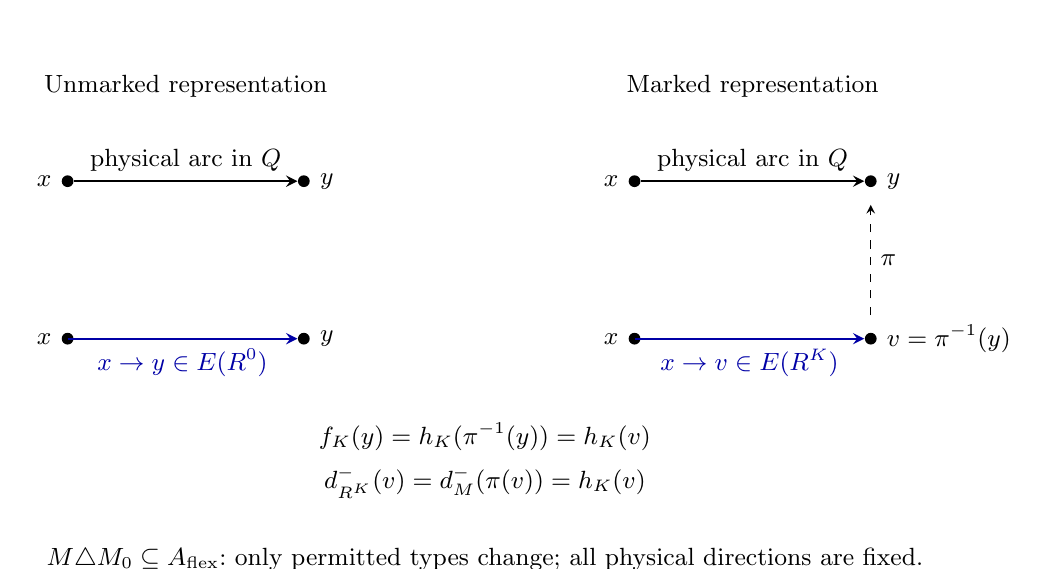
\begin{tikzpicture}[x=1cm,y=1cm,font=\small,>=stealth,
 dot/.style={circle,fill=black,inner sep=1.5pt},
 first/.style={blue!65!black,thick},
 second/.style={red!70!black,thick,dashed},
 shared/.style={green!35!black,very thick},
 spoke/.style={black!45,thin},
 tag/.style={fill=white,inner sep=1pt,font=\scriptsize}]

\node at (1.5,3.2) {Unmarked representation};
\node at (8.7,3.2) {Marked representation};
\foreach \offset in {0,7.2} {
 \begin{scope}[xshift=\offset cm]
  \node[dot,label=left:$x$] (x) at (0,2) {};
  \node[dot,label=right:$y$] (y) at (3,2) {};
  \draw[->,thick] (x)--node[above] {physical arc in $Q$} (y);
  \node[dot,label=left:$x$] (xa) at (0,0) {};
 \end{scope}
}
\node[dot,label=right:$y$] (y0) at (3,0) {};
\draw[->,first] (0,0)--node[below] {$x\to y\in E(R^0)$} (y0);
\node[dot,label={right:$v=\pi^{-1}(y)$}] (v) at (10.2,0) {};
\draw[->,first] (7.2,0)--node[below] {$x\to v\in E(R^K)$} (v);
\draw[->,dashed] (10.2,.3)--node[right] {$\pi$} (10.2,1.7);
\node[align=center] at (5.3,-1.55)
 {$f_K(y)=h_K(\pi^{-1}(y))=h_K(v)$\\[5pt]
  $d_{R^K}^-(v)=d_M^-(\pi(v))=h_K(v)$};
\node[align=center] at (5.3,-2.8)
 {$M\triangle M_0\subseteq A_{\rm flex}$:\ only permitted types change; all physical directions are fixed.};

\end{tikzpicture}
\caption{Physical and auxiliary heads in the marked indegree correction.
A physical arc $x\to y$ has auxiliary head $y$ in type $0$ and
$\pi^{-1}(y)$ in type $K$. The dashed arrow indicates $\pi$.}
\label{fig:preparation:marked-head-target}
\end{figure}

Every remaining unmarked physical edge $\{x,y\}$ satisfies
$\operatorname{dist}_\pi(x,y)>3d$: the ineligible unused edges
were assigned to the complement, and retyping was restricted to
$A_{\rm flex}$, whose arcs $x\to y$ satisfy both
$\operatorname{dist}_\pi(x,y)>3d$ and
$\operatorname{dist}_\pi(x,\pi^{-1}(y))>3d$.

\paragraph{The protected graph and the absorber.}
Since $\pi(I)=I$, a marked arc has both auxiliary endpoints in $I$
if and only if its physical endpoints lie in $I$.
No edge of $G_{\rm sel}[I]$ is used. The physical rim edges of the
approximate packing avoid $E(G_{\rm sel})$, the required inner edges
avoid $E(G_{\rm sel}[I])$, and every other newly embedded edge has
a free endpoint outside $I$.
Since $J_{\rm or}$ avoids $E(P[I])$ and every arc of
$A_{\rm flex}$ has its tail outside $I$, the physical rim edges of
$G_{\rm sel}[I]$ retain their sampled directions and assigned types.
All other residual inner edges were in $F_{\rm bad}$ and were covered.
For $w\in J$, there are no assigned matching edges, the free images
avoid $I$, and $Z_w^*$ prescribes every remaining label of
$I\setminus(O_{1,w}\cup Y_w\cup B_w\cup Z_w^{\rm occ})$.
Consequently $N_{H^0}(w)\cap I=O_{1,w}\cap I$. Since
$H^K=H_{\mathcal B}^K$, we obtain
$\mathcal R[I\cup J]=\mathcal B[I\cup J]$.

Claim~\ref{clm:long:embedding} preserves the absorber rim edges and
unmarked spokes. The marked spokes remain in $H^K$, and
$J_{\rm or}$ and $A_{\rm flex}$ avoid the absorber rim edges.
Thus $\mathcal A\subseteq\mathcal R$ with its original directions and types.

\paragraph{Changes in rim and spoke incidences.}

Let $D_H^0:=H^0\triangle H_1^0$, viewed as a bipartite graph
whose edges have type $0$. The additional type-$0$ spokes satisfy $E(H^0)\setminus E(H_1^0)\subseteq E(H_{\rm un}^{\rm raw})\cup E(H_{\rm rem}^0(\mathcal P))$.
Indeed, $N_{H^0}(w)$ avoids $Y_w$ and all approximate interval
labels and successor endpoints, which belong to $Z_w$ by
\eqref{eq:images:occupied-intervals}. The displayed union has maximum
degree at most $(2\theta+\lambda)n+2n^{3/4}$.
The spokes in $E(H_1^0)\setminus E(H^0)$ correspond to vertex images
used by the embeddings $\phi_w:Q_w\to\widehat D$. At each hub $w$ there
are at most $10\theta n$ such images. At each vertex $v$, there
are at most $\Delta(F_{\rm bad})$ assigned matching endpoints and
$\sqrt{10\theta}\,n+1$ newly chosen images. All other prescribed
images avoid $O_{1,w}$. Hence
\begin{equation}
 \Delta(D_H^0)
 \le(2\theta+\lambda)n+2n^{3/4}
 +\max\{10\theta n,\Delta(F_{\rm bad})+\sqrt{10\theta}\,n+1\}.
 \label{eq:family:long-spoke-discrepancy}
\end{equation}
Let $D_{\rm rim}$ be the typed symmetric difference of the rim
graphs of $\mathcal R$ and $\mathcal B$. By
\eqref{eq:physical:degree-comparison}, deleting physical edges of
maximum degree $h$ contributes at most $2h$ to $\Delta_*$.
A reversal or retyping contributes at most $4h$, since both the old
and new occurrences enter the symmetric difference. In particular,
changing a physical arc $x\to y$ from type $0$ to type $K$
replaces its auxiliary head $y$ by $\pi^{-1}(y)$.
The following table groups the changed rim occurrences by their
original sampling states and the two corrections.
The distance exclusions concern physical arcs $x\to y$ with
$\operatorname{dist}_\pi(x,y)\le3d$ or
$\operatorname{dist}_\pi(x,\pi^{-1}(y))\le3d$.

\begin{equation*}
\begin{array}{c|c}
\text{source of changed rim occurrences}&\text{bound}\\\hline
S\triangle S^0&2\xi n\\
F_{\rm small}&2h_{\rm small}\\
G_{\rm un}&2(2\theta n+n^{3/4})\\
\text{unused current approximate rim edges}&2\lambda n\\
\text{edges excluded by the distance conditions}&2q_d\\
\text{orientation correction}&4r_{\rm or}\\
\text{marked-type correction}&4r_{\rm type}.
\end{array}
\end{equation*}
Adding these bounds and \eqref{eq:family:long-spoke-discrepancy}
gives, for $C_*=C_*(c,C_0,C_{\rm or},\varrho_*,t)$ independent of
$\theta,d,L_{\rm cut},\lambda,\xi$,
\begin{equation*}
 \Delta_*(D_{\rm rim}\cup D_H^0)
 \le C_*\bigl((\sqrt\theta+\sqrt\xi+\lambda+1/d)n+d\bigr)+o(n).
\end{equation*}
The hierarchy and the bounded size of $\mathcal A$ therefore give,
for sufficiently large $n$,
\begin{equation}
 \Delta_*\bigl((\mathcal R-\mathcal A)\triangle\mathcal B\bigr)
 \le\Delta_*(D_{\rm rim}\cup D_H^0)+\Delta_*(\mathcal A)
 \le t_{\rm prep}n\le\zeta_{\rm rem}n.
\end{equation}

\end{proof}
\paragraph{Completing the reserved paths.}
We apply Proposition~\ref{prop:completion:marked-construction}
to the residual host in Claim~\ref{clm:long:residual}.

In this decomposition, for each $w\in U$ and $x\in Y_w$, the unique
wheel containing the marked spoke $xw$ gives a physical path from
$x$ to $\pi(x)$. These paths concatenate along each sampled interval
in $\mathcal I_w$ into its reserved path of length $cd$, with its
prescribed endpoints, by
Lemma~\ref{lem:reconstruction:paths}. Write $Q_{w,I_a}$ for the
underlying undirected physical path corresponding to
$I_a\in\mathcal I_w$. For each fixed $w$ these paths are vertex-disjoint,
have length $cd$, and satisfy $\bigcup_{I_a\in\mathcal I_w}V(Q_{w,I_a})=S_w\cup B_w=V\setminus Z_w$. Their
endpoints are $a,\pi^d(a)$, the images of
$x_0^{w,I_a},x_{cd}^{w,I_a}$ under $\widehat\phi_w$ in
Claim~\ref{clm:long:embedding}.

Each prescribed endpoint map extends to a path isomorphism
$P_{w,I_a}\to Q_{w,I_a}$. The domains meet $F_w^\circ$ only at the
prescribed endpoints, and
$V(Q_{w,I_a})\cap\widehat\phi_w(V(F_w^\circ))=\{a,\pi^d(a)\}$.
The paths $Q_{w,I_a}$ are pairwise vertex-disjoint and the endpoint
maps agree with $\widehat\phi_w$. Hence these path isomorphisms and
$\widehat\phi_w$ together give a spanning embedding
$\widehat\phi_w^+:F_w\to S$.

The complement images are pairwise edge-disjoint by
Claim~\ref{clm:long:embedding}. The paths use exactly the remaining
physical rim edges, once each, by Lemma~\ref{lem:reconstruction:paths}
and physical injectivity.
These two physical edge sets partition $E(S)$, so $E(S)=\mathop{\dot\bigcup}_{w\in U} E\bigl(\widehat\phi_w^+(F_w)\bigr)$.
This is the required decomposition.


The construction applies to every such $S$ on the same joint event,
with the same $A$. Let $\mathcal G$ be the event, determined by $S^0$,
that there exists $A\subseteq E(S^0)$ with $|A|\le B_{\rm abs}$ for
which all these corrected graphs have the asserted decomposition.
The joint event implies $\mathcal G$. Each edge of $P$ belongs to $S^0$ independently with probability
$\varrho$. Hence $\Pr_{S^0}(\mathcal G)\ge\Pr(\mathcal E_{\rm long})\ge1-\chi-n^{-10}$.
This proves the proposition.
\end{proof}

\section{Proof of Lemma~\ref{lem:family:single-copy}}

A class with very few prescribed factors is handled by removing one copy
of each factor in turn. To find a single copy, we apply
Proposition~\ref{prop:family:ordinary-preparation} or
Proposition~\ref{prop:family:long-preparation} with the same prescribed factor
at every factor index and class density one.
The class graph is then the entire input graph of the chosen proposition.


\begin{proof}[Proof of Lemma~\ref{lem:family:single-copy}]
We may assume $\vartheta+\alpha<1$. We apply
Proposition~\ref{prop:family:long-preparation} with $\alpha_0=\alpha$,
$\varrho_*=1/2$ and $\epsilon_{\max}=1$, obtaining $L_{\rm cut}$.
If at least half the vertices of $F$ lie in cycles longer than
$L_{\rm cut}$, we use Proposition~\ref{prop:family:long-preparation}.
Otherwise, the $r_*$-cycles of $F$ contain at least $n/(2L_{\rm cut})$
vertices for some $3\le r_*\le L_{\rm cut}$. We use
Proposition~\ref{prop:family:ordinary-preparation} with this $r_*$,
$\beta=1/(2L_{\rm cut})$, $\alpha_0=\alpha$, $\varrho_*=1/2$ and $\epsilon_{\max}=1$.

In either case, we choose $U$ with $|U|=D/2$ and use
$F_w=F$ for every $w\in U$, $P=G$, $\varrho=1$ and $\chi=1/4$. The initial sample satisfies $S^0=G$ deterministically. For large $n$ the event in the selected proposition
has positive probability, so its existential conclusion holds for
this graph. For the supplied sets $I$ and $A$, the graph $S=G$ satisfies
$\Delta(S\triangle S^0)=0$, $S[I]=S^0[I]$ and $A\subseteq E(S)$.
The proposition decomposes $G$ into copies of $F$, giving a spanning copy.

The cutoff $L_{\rm cut}$ is fixed before the choices for ordinary preparation.
We take the maximum of the order threshold for long preparation and
those for ordinary preparation at the finitely many eligible $r_*\le L_{\rm cut}$. The preparation bounds are uniform
over each fixed list and over all component lengths beyond their
cutoffs, so this maximum depends only on $\vartheta,\alpha$.
\end{proof}

\section{Regular edge partitions preserving prescribed subgraphs}
\label{sec:family:partition}

Propositions~\ref{prop:family:ordinary-preparation} and~\ref{prop:family:long-preparation} require an exactly regular graph
whose symmetric difference from its independent edge sample has
small maximum degree. They also require equality on
a specified induced inner graph and preservation of the reserved absorber.
Lemma~\ref{lem:family:partition} supplies these properties for all classes simultaneously.
A related regular edge partition appears in \cite[Lemma~9.1]{KeevashStaden2022}.
The cut and redistribution arguments here also preserve every
specified inner graph and absorber edge.


\begin{proof}[Proof of Lemma~\ref{lem:family:partition}]
\startlocalclaims
For the given inputs of Lemma~\ref{lem:family:partition},
independently of the edge colors, orient every edge of $P$
fairly and independently, obtaining $D_0$.

\begin{localclaim}\label{clm:partition:balanced-orientation}
There is an event $\mathcal E_{\rm or}$, determined by $D_0$, with
probability at least $1-n^{-10}$, on which the following holds
for every graph $F$ on $V(P)$ with $\Delta(F)\le\alpha n/100$.
There is an orientation $\vec P$ of $P$ such that $d_{\vec P}^+(v)=d_{\vec P}^-(v)=d_P(v)/2$ for all $v\in V(P)$. The graph $J$ of
edges on which $\vec P,D_0$ differ satisfies $\Delta(J)\le4n^{4/5}$ and $E(J)\cap E(F)=\varnothing$.
\end{localclaim}
\begin{proof}
Let $\mathcal E_{\rm or}$ be the event that
$d_{D_0}^+(v)=d_P(v)/2\pm n^{3/5}$ for every $v$ and
$|N_{D_0}^+(x)\cap N_{D_0}^-(y)|\ge\alpha n/4$ for all $x\ne y$.
Since $|N_P(x)\cap N_P(y)|\ge2\alpha n$ and the paths
$x\to z\to y$ occur independently over these common neighbors
with probability $1/4$, McDiarmid's bounded-differences inequality (Theorem~\ref{thm:prelim:bounded-differences}),
Chernoff's inequality (Lemma~\ref{lem:prelim:chernoff}) and a union bound give
\begin{equation}
 \Pr(\mathcal E_{\rm or}^c)
 \le2n\exp(-2n^{1/5})+n^2\exp(-\alpha n/16)\le n^{-10}.
 \label{eq:prob:lem:new:balanced-orientation}
\end{equation}
Since all degrees of $P$ are even, on $\mathcal E_{\rm or}$
we apply Lemma~\ref{lem:simp:orientation-routing}
with $G=P$, $E_{\rm el}=E(P)$, $a=n^{3/5}$,
$\beta=\alpha/4$, $L=\lceil n^{4/5}\rceil$ and $f=\alpha n/100$.
Its numerical hypothesis holds since
$na/L+2a+4L+2f=o(n)+\alpha n/50<\beta n$.
The lemma gives the required $\vec P$ with $\Delta(J)\le a+2L\le4n^{4/5}$,
for every $F$ with $\Delta(F)\le\alpha n/100$.
\end{proof}

Put $Z:=\bigcup_bP[I_b]$ and $D_a^{\rm raw}:=D_0[E(S_a^0)]$.
Because the $I_b$ precede the colors and $D_0$ is independent of them,
Hoeffding's inequality for independent sums (Theorem~\ref{thm:prelim:bounded-differences}) and a union bound give, simultaneously for all $a,v$,
\begin{equation*}
 \Delta(S_a^0\cap Z)\le\varrho_a\epsilon_\Sigma n+n^{3/5},\qquad
 d_{D_a^{\rm raw}}^\pm(v)=m_a\pm n^{3/5}.
\end{equation*}
Fix any permitted family $(A_a)$, and let $F$ be the graph on $V(P)$
with $E(F):=E(Z)\cup\bigcup_a A_a$. Then
$\Delta(F)\le\epsilon_\Sigma n+B_0\le\alpha n/100$ for large $n$.
Claim~\ref{clm:partition:balanced-orientation} gives a balanced
orientation $\vec P$ that differs from $D_0$ on a graph of maximum degree
at most $4n^{4/5}$ and on no edge of $F$.
For $D_a^0:=\vec P[E(S_a^0)]$, it follows that
$d_{D_a^0}^\pm(v)=m_a\pm e_n$, where $e_n:=5n^{4/5}$.

For $X,Y\subseteq V(P)$, let $e_{\vec P}(X,Y)$ count the arcs from $X$
to $Y$, even when $X\cap Y\ne\varnothing$. These are the cut counts
in the bipartite representation of $\vec P$. Put
$\delta_a:=\min\{\alpha/32,\varrho_a/512\}$ and
$h_a:=\alpha\varrho_a/128$. Each orientation and color pair in
$D_a^{\rm raw}$ has probability $\varrho_a/2$.
Outside the exceptional event estimated below, the following
bound holds simultaneously for every color $a$ and every
$X,Y\subseteq V(P)$:
\begin{equation}
 e_{D_a^{\rm raw}}(X,Y)\ge2h_an\min\{|X|,|Y|\}
 \quad\hbox{if }|X|+|Y|>(1-2\delta_a)n.
 \label{eq:family:raw-partition-cut}
\end{equation}
If $\min\{|X|,|Y|\}\le\varrho_an/32$, the larger set omits at most
$(\varrho_a/32+2\delta_a)n$ vertices. The indegree and outdegree
bounds for $D_a^{\rm raw}$ give
at least $(\varrho_a/4-\varrho_a/32-2\delta_a-o(1))n
\ge\varrho_an/8$ neighbors per vertex of the smaller set,
which proves \eqref{eq:family:raw-partition-cut}.
Otherwise both sets have size greater than $\varrho_an/32$, and
$\max\{|X|,|Y|\}>(1/2-\delta_a)n$. Thus
\begin{equation*}
 \mathbb E e_{D_a^{\rm raw}}(X,Y)
 \ge\tfrac12\varrho_a(\alpha-\delta_a)n\min\{|X|,|Y|\}.
\end{equation*}
The contributions of distinct physical edges are independent
$\{0,1\}$-valued variables, also when $X,Y$ overlap.
Chernoff's inequality (Lemma~\ref{lem:prelim:chernoff}) bounds the failure probability in
\eqref{eq:family:raw-partition-cut} by $\exp(-c_{{\rm cut},a}n^2)$ for a fixed
$c_{{\rm cut},a}=c_{{\rm cut},a}(\alpha,\underline\varrho_a)>0$. A union bound covers
the at most $4^n$ pairs $(X,Y)$.

Removing protected edges and allowing for reversals loses at most
$(\varrho_a\epsilon_\Sigma n+n^{3/5}+B_0+4n^{4/5})\min\{|X|,|Y|\}$ from a cut. By the choice of
$\epsilon_\Sigma$, the digraph $D_a^0-F$ therefore satisfies
\begin{equation}
 e_{D_a^0-F}(X,Y)\ge h_an\min\{|X|,|Y|\}
 \quad\hbox{if }|X|+|Y|>(1-2\delta_a)n.
 \label{eq:family:allowed-partition-cut}
\end{equation}
After division by $n\min\{|X|,|Y|\}$, the contribution
$\varrho_a\epsilon_\Sigma$ from the prescribed inner graphs satisfies
$\varrho_a\epsilon_\Sigma/h_a=128\epsilon_\Sigma/\alpha$.
This ratio is independent of $\varrho_a$. The remaining normalized
loss tends to zero as $n\to\infty$ with the later inputs fixed.

We choose $q_*>0$, after the stated errors and density bounds, with
\begin{equation*}
 q_*\le\min_a\{\xi_a/16,\alpha\underline\varrho_a/2048,
                             \underline\varrho_a/64\},
 \qquad q:=\lfloor q_*n\rfloor.
\end{equation*}
We will lower the indegree and outdegree of each $D_a^0$ to $m_a-q$,
then repartition the deleted arcs to give indegree and outdegree $m_a$
in every color.
For sufficiently large $n$, the fixed choice of $q_*$ gives
\begin{equation*}
 e_n<q\le\min_a m_a,\quad
 2e_n/(q-e_n)\le\min_a\delta_a,\quad
 q+e_n\le\tfrac12\min_a h_a n.
\end{equation*}
We prescribe outgoing and incoming deletion demands
$f_a(v):=d^+_{D_a^0}(v)-(m_a-q)$ and
$g_a(v):=d^-_{D_a^0}(v)-(m_a-q)$.
Their totals agree. Each demand and their common mean belong to
$[q-e_n,q+e_n]$, so the relative deviations are at most $2e_n/(q-e_n)$
and the total is at most $n(q+e_n)$.
We apply Lemma~\ref{lem:prelim:normalized-demands} to the bipartite
representation of $D_a^0-F$, with both part sizes equal to $n$,
$h=h_a$, $\delta_0=\delta_a$, $\delta=2e_n/(q-e_n)$ and
$M=\sum_v f_a(v)$. We use demands $f_a$ on tail copies and $g_a$
on head copies. The cut bound is
\eqref{eq:family:allowed-partition-cut}, and
$M\le n(q+e_n)\le h_an^2/2$.
The integral conclusion gives $T_a\subseteq D_a^0-F$ with these degrees.
The remaining digraph $C_a:=D_a^0-T_a$ has in- and outdegree
$m_a-q$ at every vertex.

Since $\vec P$ is balanced, $T:=\dot\bigcup_a T_a$ has in- and
outdegree $kq$. By repeated application of Hall's theorem
(Theorem~\ref{thm:prelim:hall}), its $kq$-regular bipartite
representation decomposes into $kq$ perfect matchings. Assigning $q$ matchings to each color gives a partition
$T=\dot\bigcup_a Q_a$ with $d_{Q_a}^+(v)=d_{Q_a}^-(v)=q$.
Let $S_a$ be the underlying graph of $C_a\cup Q_a$. Then $E(P)=\mathop{\dot\bigcup}_a E(S_a)$ and $d_{S_a}(v)=2m_a$ for all $v \in V(P)$.
The removed physical degree is at most $2q+2e_n$ and the added
degree is $2q$, so
$\Delta(S_a\triangle S_a^0)\le4q+2e_n\le\xi_an$.
Since $E_{\rm phys}(T_a)\cap E(F)=\varnothing$ for every $a$,
every edge of $F$ remains in
its original color. Hence $S_a[I_b]=S_a^0[I_b]$ for all $a,b$
and $A_a\subseteq E(S_a)$. The auxiliary orientation $\vec P$ only
constructs this undirected partition and does not alter the sampled directions
in the completion samples.

Let $\mathcal G$ be the joint event of colors and directions on which
$\mathcal E_{\rm or}$, the degree bounds and
\eqref{eq:family:raw-partition-cut} hold.
The probability that any of the $O(kn)$ degree estimates or any
cut estimate in \eqref{eq:family:raw-partition-cut} fails is at most
$O(kn\exp(-a_0n^{1/5}))+k4^n\exp(-a_1n^2)$
for fixed $a_0,a_1>0$.
Combining these bounds with \eqref{eq:prob:lem:new:balanced-orientation}
gives $\Pr(\mathcal G^c)\le n^{-10}$ for sufficiently large $n$.
On $\mathcal G$, the construction works for every permitted family $(A_a)$.
If $\mathcal E$ is the event that the colors admit the required
partition for every such family, then
$\mathcal G\subseteq\mathcal E\times\Omega_{\rm or}$, where
$\Omega_{\rm or}$ is the orientation sample space. Thus
$\Pr_{\rm colors}(\mathcal E)\ge\Pr(\mathcal G)\ge1-n^{-10}$.
\end{proof}




% End corrected_original_cover

\clearpage
\section{Concluding remarks}
\label{sec:concluding}

\subsection{Fractional decompositions in cyclic-partite graphs}
\label{subsec:intro:cyclic-fractional}

Section~\ref{sec:writing:cyclic-fractional} develops the path
weightings and endpoint-matrix construction used to obtain long-cycle
weights in the proof of Theorem~\ref{thm:new:prescribed-factor}.
Here we present further applications of these ideas to fractional
decompositions in cyclic-partite graphs, giving results of independent
interest and discussing related conjectures.
Recall from Section~\ref{sec:writing:cyclic-fractional} that
an $\ell$-cyclic graph $G$ has specified vertex classes
$V_0,\ldots,V_{\ell-1}$ and edges only between consecutive
classes, with indices modulo $\ell$.
It is locally balanced when
$d_G(v,V_{i-1})=d_G(v,V_{i+1})$ for every $v\in V_i$.
For such a graph, $\delta_{\rm cyc}(G)$ is the minimum of these
common degrees. A part-respecting $C_\ell$ meets each class once.

For $\ell=3$, the corresponding integral decomposition problem is
the~\emph{tripartite Nash-Williams conjecture}~\cite[Conjecture~1.3, $r=3$]{BKLOT2017}.

\begin{conjecture}[Tripartite Nash-Williams conjecture]\label{conj:tripartite}
For all sufficiently large $n$, every locally balanced tripartite graph with three parts of size $n$ and minimum cyclic degree at least $3n/4$ has a $K_3$-decomposition.
\end{conjecture}



Let\phantomsection\label{gls:partite-fractional-triangle-threshold} $\widehat\delta^*_{K_3}$ be the infimum of the real numbers $c$ such that every locally balanced tripartite graph with parts of size $n$ and minimum cyclic degree at least $cn$ has a fractional $K_3$-decomposition whenever $n$ is sufficiently large.
Using the result by Haxell and R\"odl~\cite{HaxellRodl2001}, Barber, K\"uhn, Lo, Osthus and Taylor~\cite[Corollary~1.6]{BKLOT2017} proved that, for every $\varepsilon>0$
and all sufficiently large $n$, the local balance condition and $\delta_{\rm cyc}(G)\ge (\widehat\delta^*_{K_3}+\varepsilon)n$ ensure a $K_3$-decomposition. Thus $\widehat\delta^*_{K_3}=3/4$ would imply an asymptotic version of Conjecture~\ref{conj:tripartite}.

Several advances have been made toward Conjecture~\ref{conj:tripartite}.
For every $r\ge3$, Montgomery~\cite{Montgomery2017Partite}
proved that a balanced $r$-partite graph with parts of size $n$
has a fractional $K_r$-decomposition if each vertex has the same
number of neighbors in every other part and this number is at least
$(1-1/(10^6r^3))n$.
Longbrake, Simkin, Yepremyan and Zheng~\cite{LongbrakeEtAl2026Partite}
recently weakened this degree requirement to $(1-1/(30r^2))n$
for all sufficiently large $n$.

For $r=3$, Bowditch and Dukes~\cite{BowditchDukes2019} proved $\widehat\delta^*_{K_3} \le 0.96$.
Recently, Yu and Feng~\cite{YuFeng2026} proved $\widehat\delta^*_{K_3} \le 23/25$, He and Cheng~\cite{HeCheng2026} proved $\widehat\delta^*_{K_3} \le 0.8$, and Allsop, Bowtell, Lesgourgues and Petrova~\cite{ABLP2026} proved $\widehat\delta^*_{K_3} < 0.769$.

For general cycle lengths, the corresponding candidate threshold is
$q_\ell n$, where $q_\ell:=1/2+1/(2\ell-2)$ for $\ell\ge3$.

\begin{conjecture}\label{conj:odd_cyclic_threshold}
Let $\ell \ge3$ be an integer, and let $n \geq 1$ be an integer.
Let $G$ be a locally balanced $\ell$-cyclic graph with specified classes
$V_0,\ldots,V_{\ell-1}$ of size $n$. 
If $\delta_{\rm cyc}(G)\ge q_\ell n = (1/2 + 1/(2\ell-2))n$, then there is a fractional part-respecting $C_\ell$-decomposition
$\omega:\mathcal C^{\rm part}_\ell(G)\to\mathbb R_{\ge0}$ of $G$.
\end{conjecture}

Here, the coefficient $q_\ell$ is best possible (see Proposition~\ref{doLpart:prop:sharp}).
For $\ell=3$, this is the fractional analog of Conjecture~\ref{conj:tripartite}. 
For odd $\ell\ge5$, we prove Conjecture~\ref{conj:odd_cyclic_threshold} under the stronger degree condition $\delta_{\rm cyc}(G)\ge q_{\ell-1}n$ (see Theorem~\ref{doLpart:thm:odd}). Recently, the first two authors~\cite{KM2026_long} proved Conjecture~\ref{conj:odd_cyclic_threshold} for all odd integers $\ell \geq \ell_0$, where $\ell_0$ is a large constant.

We determine this fractional part-respecting cycle decomposition
threshold for every even $\ell\ge4$.

\begin{theorem}\label{doLpart:thm:main}
Let $k\ge2$ and $n\ge1$ be integers, and let $\ell:=2k$.
Let $G$ be a locally balanced $\ell$-cyclic graph with specified classes
$V_0,\ldots,V_{\ell-1}$ of size $n$. Suppose
\begin{equation}
 \label{doLpart:eq:main-threshold}
 \delta_{\rm cyc}(G)\ge q_\ell n = \frac{k}{2k-1}n.
\end{equation}
Then there is a fractional part-respecting $C_\ell$-decomposition
$\omega:\mathcal C^{\rm part}_\ell(G)\to\mathbb R_{\ge0}$ of $G$.
\end{theorem}

In the proof of Theorem~\ref{doLpart:thm:main}, we use Brouwer's fixed-point theorem (Theorem~\ref{thm:prelim:brouwer}) to choose path weightings whose endpoint distributions agree around the cycle. This agreement allows the paths to be joined into cycles while preserving their edge loads.
The proof is given in Appendix~\ref{app:cyclic:even}.

\begin{theorem}\label{doLpart:thm:odd}
Let $k\ge2$ and $n\ge1$ be integers, and let $\ell:=2k+1$.
Let $G$ be a locally balanced $\ell$-cyclic graph with specified
classes $V_0,\ldots,V_{\ell-1}$ of size $n$. If $\delta_{\rm cyc}(G)\ge kn/(2k-1)$ then $G$ has a fractional part-respecting $C_\ell$-decomposition.
\end{theorem}

The proof extends the even-length construction by combining
two-edge paths with a closing edge from $G[V_{\ell-1},V_0]$.
It is given in Appendix~\ref{app:cyclic:odd}.


\paragraph{Related conjectures and results.}

Daykin and H\"aggkvist~\cite{DaykinHaggkvist1983} conjectured that every partial Latin square of order $n$ in which each row, column and symbol occurs in at most $n/4$ entries is completable. Earlier work on the Daykin--H\"aggkvist conjecture includes Chetwynd and H\"aggkvist~\cite{ChetwyndHaggkvist1985}, Gustavsson~\cite{Gustavsson1991} and Bartlett~\cite{Bartlett2013}.
Wanless~\cite{Wanless2002} gave noncompletable examples in which
each row, column and symbol occurs at most $n/4+1$ times.

To see how the Daykin--H\"aggkvist conjecture is related to Conjecture~\ref{conj:tripartite}, consider three parts of $K_{n,n,n}$ representing the rows, columns and symbols of a Latin square of order $n$, and delete the triangle associated with each filled entry. The remaining graph is locally balanced, has cyclic degree at least $3n/4$, and has a triangle decomposition if and only if the partial Latin square is completable. Therefore, Conjecture~\ref{conj:tripartite} implies the Daykin--H\"aggkvist conjecture for all sufficiently large $n$.

For even cycles that need not be part-respecting, Sun, Feng and
Yu~\cite{SunFengYu2026} determined the asymptotic $C_{2k}$-decomposition
thresholds for $r$-partite graphs $G$ with parts $V_1,\ldots,V_r$
satisfying $\max_i|V_i|\le2\min_i|V_i|$. Here, degree is measured by
$\min\{d_G(v,V_i)/|V_i|:i\in[r],\ v\in V(G)\setminus V_i\}$.
Subject to the necessary cycle-divisibility conditions, the thresholds
are $2/3$ for $C_4$ and $1/2$ for $C_{2k}$ with $k\ge3$,
extending Taylor's bipartite result~\cite[Theorem~1.3]{taylor2019}.



\clearpage
\section*{Acknowledgments}
We would like to thank Daniela K\"{u}hn, Deryk Osthus, Vincent Pfenninger, and Jigang Choi for valuable discussions about this project.
We are also grateful to Allan Lo and Katherine Staden for their many helpful comments on the third author's PhD thesis, which forms part of this paper.

\section*{Statement on the use of AI}
The project began in 2022, when the authors started working on the degree
threshold for resolvable cycle decompositions (Corollary~\ref{cor:resolvable_threshold}) and obtained related results. A special case of
this work appeared in the third author's PhD thesis. Extending these ideas,
the authors resolved the long Oberwolfach problem for robust
outexpanders and robust expanders. The proof ideas for both
Corollary~\ref{cor:resolvable_threshold} and this resolution of the long Oberwolfach
problem are entirely due to the authors. These include approximate
wheel-decompositions, cover-down lemmas, the construction of absorbers via
transformers, and absorbers for cycle factors, all in the setting of
ordinary cycle and wheel decompositions treated in the current manuscript.

The authors also proved several results on fractional
decompositions in cyclic-partite graphs, described in
Section~\ref{subsec:intro:cyclic-fractional} and Appendix~\ref{app:cyclic}
of this paper. These results and their corresponding random
sparsification extensions are needed to adapt the high-level strategy of
Glock, Joos, Kim, K\"uhn and Osthus~\cite{GlockEtAl2021Oberwolfach} to prove
Theorem~\ref{thm:new:prescribed-factor} for a single prescribed 2-factor $F$,
particularly for constructing the absorbers. However, this approach also
requires the case $\ell=3$ of Conjecture~\ref{conj:odd_cyclic_threshold} of this paper (the fractional version of the tripartite Nash--Williams conjecture) and its random sparsification results, which the
authors were unable to prove.

The authors therefore considered a different strategy for proving
Theorem~\ref{thm:new:prescribed-factor}. After understanding the proof of
Keevash and Staden~\cite{KeevashStaden2022}, they realized that this
strategy does not require the case $\ell=3$ of
Conjecture~\ref{conj:odd_cyclic_threshold} or its random sparsification results.
Instead, the ingredients they had already developed for ordinary cycle
and wheel decompositions and fractional decompositions in cyclic-partite
graphs suffice to deduce the main ingredients for the marked variants of
these decompositions used in the manuscript. To help carry out this
adaptation, the authors supplied these ingredients to ChatGPT 5.6 Sol
and ChatGPT 6 Astra and guided these models in assembling them using
the authors' existing ideas, carrying out tedious computations, and
writing technical parts of the proofs.
The authors take full responsibility for the entire content and integrity of this paper.

\begin{thebibliography}{10}

\bibitem{ABLP2026}
Jack Allsop, Candida Bowtell, Thomas Lesgourgues, and Kalina Petrova.
\newblock Improved bounds on completion of partial Latin squares.
\newblock arXiv preprint, 2026.
\newblock \url{https://arxiv.org/abs/2609.37877}.

\bibitem{BarberEtAl2020Minimalist}
Ben Barber, Stefan Glock, Daniela K{\"u}hn, Allan Lo, Richard Montgomery, and
  Deryk Osthus.
\newblock Minimalist designs.
\newblock {\em Random Structures \& Algorithms}, 57(1):47--63, 2020.
\newblock \url{https://arxiv.org/abs/1808.06956}.

\bibitem{BKLMO2017Fractional}
Ben Barber, Daniela K{\"u}hn, Allan Lo, Richard Montgomery, and
  Deryk Osthus.
\newblock Fractional clique decompositions of dense graphs and hypergraphs.
\newblock {\em Journal of Combinatorial Theory, Series B}, 127:148--186, 2017.
\newblock \url{https://doi.org/10.1016/j.jctb.2017.05.005}.
\newblock \url{https://arxiv.org/abs/1507.04985}.

\bibitem{BKLO2016}
Ben Barber, Daniela K{\"u}hn, Allan Lo, and Deryk Osthus.
\newblock Edge-decompositions of graphs with high minimum degree.
\newblock {\em Advances in Mathematics}, 288:337--385, 2016.
\newblock \url{https://doi.org/10.1016/j.aim.2015.09.032}.

\bibitem{BKLOT2017}
Ben Barber, Daniela K{\"u}hn, Allan Lo, Deryk Osthus, and Amelia Taylor.
\newblock Clique decompositions of multipartite graphs and completion of
  {Latin} squares.
\newblock {\em Journal of Combinatorial Theory, Series A}, 151:146--201, 2017.
\newblock \url{https://arxiv.org/abs/1603.01043}.

\bibitem{Bartlett2013}
Padraic Bartlett.
\newblock Completions of $\epsilon$-dense partial Latin squares.
\newblock {\em Journal of Combinatorial Designs}, 21(10):447--463, 2013.
\newblock \url{https://arxiv.org/abs/1205.1558}.

\bibitem{BowditchDukes2019}
Flora C.~Bowditch and Peter J.~Dukes.
\newblock Fractional triangle decompositions of dense 3-partite graphs.
\newblock {\em Journal of Combinatorics}, 10(2):255--282, 2019.
\newblock \url{https://arxiv.org/abs/1510.08998}.

\bibitem{Brouwer1911}
L.~E.~J. Brouwer.
\newblock {\"U}ber Abbildung von Mannigfaltigkeiten.
\newblock {\em Mathematische Annalen}, 71:97--115, 1911.
\newblock \url{https://doi.org/10.1007/BF01456931}.

\bibitem{BryantEtAl2026}
Darryn Bryant, Peter Dukes, Daniel Horsley, Barbara Maenhaut, and Richard
  Montgomery.
\newblock On decomposition thresholds for odd-length cycles and other
  tripartite graphs.
\newblock {\em Journal of Combinatorial Theory, Series B}, 180:94--110, 2026.
\newblock \url{https://arxiv.org/abs/2411.17232}.

\bibitem{Caratheodory1911}
C.~Carath\'eodory.
\newblock {\"U}ber den Variabilit{\"a}tsbereich der Fourier'schen Konstanten von
positiven harmonischen Funktionen.
\newblock {\em Rendiconti del Circolo Matematico di Palermo}, 32:193--217, 1911.
\newblock \url{https://doi.org/10.1007/BF03014795}.

\bibitem{CKKO2019}
Padraig Condon, Jaehoon Kim, Daniela K{\"u}hn, and Deryk Osthus.
\newblock A bandwidth theorem for approximate decompositions.
\newblock {\em Proceedings of the London Mathematical Society}, 118(6):1393--1449, 2019.
\newblock \url{https://arxiv.org/abs/1712.04562}.

\bibitem{Chan2010}
Justin H.~Chan.
\newblock {\em Asymptotic existence results on specific graph decompositions}.
\newblock M.Sc. thesis, University of Victoria, 2010.
\newblock \url{https://www.collectionscanada.gc.ca/obj/thesescanada/vol2/BVIV/TC-BVIV-2909.pdf}.

\bibitem{ChetwyndHaggkvist1985}
Amanda Chetwynd and Roland H\"aggkvist.
\newblock Completing partial $n\times n$ Latin squares where each row,
column and symbol is used at most $cn$ times.
\newblock Preprint (research report), 1985.

\bibitem{CsabaEtAl2016}
B{\'e}la Csaba, Daniela K{\"u}hn, Allan Lo, Deryk Osthus, and Andrew Treglown.
\newblock Proof of the {$1$}-factorization and {Hamilton} decomposition conjectures.
\newblock {\em Memoirs of the American Mathematical Society}, 244(1154), 2016.
\newblock \url{https://arxiv.org/abs/1401.4159}.

\bibitem{DaykinHaggkvist1983}
David E.~Daykin and Roland H\"aggkvist.
\newblock Completion of sparse partial Latin squares.
\newblock In B.~Bollob{\'a}s, editor, {\em Graph Theory and Combinatorics}
  (Cambridge, 1983), pages 127--132. Academic Press, London, 1984.

\bibitem{DelcourtHendersonLesgourguesPostle2025}
Michelle Delcourt, Cicely Henderson, Thomas Lesgourgues, and Luke Postle.
\newblock {Erd\H{o}s} meets {Nash-Williams}.
\newblock arXiv preprint, 2025.
\newblock \url{https://arxiv.org/abs/2507.23624v1}.

\bibitem{DelcourtPostleRefined2024}
Michelle Delcourt and Luke Postle.
\newblock Refined absorption: A new proof of the existence conjecture.
\newblock arXiv preprint, 2024.
\newblock \url{https://arxiv.org/abs/2402.17855}.

\bibitem{DelcourtPostle2026}
Michelle Delcourt and Luke Postle.
\newblock A proof of {Nash-Williams}' conjecture.
\newblock arXiv preprint, 2026.
\newblock \url{https://arxiv.org/abs/2606.11178v1}.

\bibitem{DukesLing2007}
Peter Dukes and Alan C.~H.~Ling.
\newblock Asymptotic existence of resolvable graph designs.
\newblock {\em Canadian Mathematical Bulletin}, 50(4):504--518, 2007.

\bibitem{EGJ2020}
Stefan Ehard, Stefan Glock, and Felix Joos.
\newblock Pseudorandom hypergraph matchings.
\newblock {\em Combinatorics, Probability and Computing}, 29(6):868--885, 2020.
\newblock \url{https://doi.org/10.1017/S0963548320000280}.

\bibitem{FLM2017}
Asaf Ferber, Choongbum Lee, and Frank Mousset.
\newblock Packing spanning graphs from separable families.
\newblock {\em Israel Journal of Mathematics}, 219(2):959--982, 2017.
\newblock \url{https://arxiv.org/abs/1512.08701}.

\bibitem{FordFulkerson1956}
L.~R.~Ford, Jr. and D.~R.~Fulkerson.
\newblock Maximal flow through a network.
\newblock {\em Canadian Journal of Mathematics}, 8:399--404, 1956.
\newblock \url{https://doi.org/10.4153/CJM-1956-045-5}.

\bibitem{FordFulkerson1957}
L.~R.~Ford, Jr. and D.~R.~Fulkerson.
\newblock A simple algorithm for finding maximal network flows and an
application to the Hitchcock problem.
\newblock {\em Canadian Journal of Mathematics}, 9:210--218, 1957.
\newblock \url{https://doi.org/10.4153/CJM-1957-024-0}.

\bibitem{GlockGouldJoosKuhnOsthus2021}
Stefan Glock, Stephen Gould, Felix Joos, Daniela K{\"u}hn, and Deryk Osthus.
\newblock Counting {Hamilton} cycles in {Dirac} hypergraphs.
\newblock {\em Combinatorics, Probability and Computing}, 30(4):631--653, 2021.
\newblock \url{https://arxiv.org/abs/1911.08887}.

\bibitem{GlockEtAl2021Oberwolfach}
Stefan Glock, Felix Joos, Jaehoon Kim, Daniela K{\"u}hn, and Deryk Osthus.
\newblock Resolution of the {Oberwolfach} problem.
\newblock {\em Journal of the European Mathematical Society}, 23(8):2511--2547,
  2021.
\newblock \url{https://arxiv.org/abs/1806.04644}.

\bibitem{GlockThreshold2019}
Stefan Glock, Daniela K{\"u}hn, Allan Lo, Richard Montgomery, and Deryk Osthus.
\newblock On the decomposition threshold of a given graph.
\newblock {\em Journal of Combinatorial Theory, Series B}, 139:47--127, 2019.
\newblock \url{https://arxiv.org/abs/1603.04724}.

\bibitem{GlockEtAl2023Designs}
Stefan Glock, Daniela K{\"u}hn, Allan Lo, and Deryk Osthus.
\newblock The existence of designs via iterative absorption:
  hypergraph {$F$}-designs for arbitrary {$F$}.
\newblock {\em Memoirs of the American Mathematical Society},
  284(1406), v+131 pp., 2023.
\newblock \url{https://arxiv.org/abs/1611.06827}.

\bibitem{GlockKuhnOsthus2021Survey}
Stefan Glock, Daniela K{\"u}hn, and Deryk Osthus.
\newblock Extremal aspects of graph and hypergraph decomposition problems.
\newblock In {\em Surveys in Combinatorics 2021}, volume 470 of {\em London
  Mathematical Society Lecture Note Series}, pages 235--265. Cambridge
  University Press, 2021.
\newblock \url{https://arxiv.org/abs/2008.00926}.

\bibitem{GranetHorsley2026}
Bertille Granet and Daniel Horsley.
\newblock Determining decomposition thresholds for long odd cycles.
\newblock arXiv preprint, 2026.
\newblock \url{https://arxiv.org/abs/2606.21548v1}.

\bibitem{GranetHorsleySantrio2026}
Bertille Granet, Daniel Horsley, and Jeffrey N. Santrio.
\newblock A note on decompositions into 3-chromatic graphs.
\newblock arXiv preprint, 2026.
\newblock \url{https://arxiv.org/abs/2610.41266v1}.

\bibitem{Gustavsson1991}
Torbj\"orn Gustavsson.
\newblock {\em Decompositions of large graphs and digraphs with high minimum degree}.
\newblock PhD thesis, Lund University, 1991.

\bibitem{guy1971}
Richard K.~Guy.
\newblock Unsolved combinatorial problems.
\newblock In D.~J.~A. Welsh, editor, {\em Combinatorial Mathematics and Its Applications}, pages 121--127. Academic Press, London, 1971.

\bibitem{Hall1935}
P.~Hall.
\newblock On representatives of subsets.
\newblock {\em Journal of the London Mathematical Society}, 10(1):26--30, 1935.
\newblock \url{https://doi.org/10.1112/jlms/s1-10.37.26}.

\bibitem{HaxellRodl2001}
Penny E.~Haxell and Vojt\v{e}ch R\"odl.
\newblock Integer and fractional packings in dense graphs.
\newblock {\em Combinatorica}, 21(1):13--38, 2001.

\bibitem{Hoeffding1963}
Wassily Hoeffding.
\newblock Probability inequalities for sums of bounded random variables.
\newblock {\em Journal of the American Statistical Association}, 58(301):13--30, 1963.
\newblock \url{https://doi.org/10.1080/01621459.1963.10500830}.

\bibitem{HHW2026}
Jianfeng Hou, Caiyun Hu, and Hezhi Wang.
\newblock On decomposition thresholds for odd cycles.
\newblock arXiv preprint, 2026.
\newblock \url{https://arxiv.org/abs/2610.23471v2}.

\bibitem{HeCheng2026}
Hengzhi He and Guang Cheng.
\newblock Fractional triangle decompositions at partite minimum degree $4n/5$.
\newblock arXiv preprint, 2026.
\newblock \url{https://arxiv.org/abs/2609.31758}.

\bibitem{JK2022}
Felix Joos and Marcus K\"{u}hn.
\newblock Fractional cycle decompositions in hypergraphs.
\newblock {\em Random Structures \& Algorithms}, 61(3):425--443, 2022.
\newblock \url{https://doi.org/10.1002/rsa.21070}.

\bibitem{JKS2023}
Felix Joos, Marcus K\"{u}hn, and Bjarne Sch{\"u}lke.
\newblock Decomposing hypergraphs into cycle factors.
\newblock {\em Journal of Combinatorial Theory, Series B}, 158:136--175, 2023.
\newblock \url{https://arxiv.org/abs/2104.06333}.

\bibitem{KangEtAl2023Latin}
Dong Yeap Kang, Tom Kelly, Daniela K{\"u}hn, Abhishek Methuku,
  and Deryk Osthus.
\newblock Thresholds for {Latin} squares and {Steiner} triple systems:
  bounds within a logarithmic factor.
\newblock {\em Transactions of the American Mathematical Society},
  376:6623--6662, 2023.
\newblock \url{https://doi.org/10.1090/tran/8954}.

\bibitem{KangEtAl2024Matchings}
Dong Yeap Kang, Tom Kelly, Daniela K{\"u}hn, Deryk Osthus,
  and Vincent Pfenninger.
\newblock Perfect matchings in random sparsifications of {Dirac} hypergraphs.
\newblock {\em Combinatorica}, 44:1233--1266, 2024.
\newblock \url{https://arxiv.org/abs/2211.01325}.

\bibitem{KM2026_long}
Dong Yeap Kang and Abhishek Methuku.
\newblock Fractional long part-respecting cycle decompositions of locally balanced cyclic partite graphs.
\newblock Preprint, 2026.

\bibitem{KeevashDesigns2014}
Peter Keevash.
\newblock The existence of designs.
\newblock {\em Annals of Mathematics}, to appear.
\newblock \url{https://annals.math.princeton.edu/articles/22929}.
\newblock \url{https://arxiv.org/abs/1401.3665}.

\bibitem{KeevashDesignsII2018}
Peter Keevash.
\newblock The existence of designs II.
\newblock arXiv preprint, 2018.
\newblock \url{https://arxiv.org/abs/1802.05900}.

\bibitem{KeevashStaden2022}
Peter Keevash and Katherine Staden.
\newblock The generalised {Oberwolfach} problem.
\newblock {\em Journal of Combinatorial Theory, Series B}, 152:281--318, 2022.
\newblock \url{https://doi.org/10.1016/j.jctb.2021.09.007}.

\bibitem{KKOT2019}
Jaehoon Kim, Daniela K{\"u}hn, Deryk Osthus, and Mykhaylo Tyomkyn.
\newblock A blow-up lemma for approximate decompositions.
\newblock {\em Transactions of the American Mathematical Society}, 371(7):4655--4742, 2019.
\newblock \url{https://arxiv.org/abs/1604.07282}.

\bibitem{KnoxKuhnOsthus2015}
Fiachra Knox, Daniela K{\"u}hn, and Deryk Osthus.
\newblock Edge-disjoint {Hamilton} cycles in random graphs.
\newblock {\em Random Structures \& Algorithms}, 46:397--445, 2015.
\newblock \url{https://arxiv.org/abs/1104.4412}.

\bibitem{KuhnOsthus2013Hamilton}
Daniela K{\"u}hn and Deryk Osthus.
\newblock Hamilton decompositions of regular expanders: a proof of
  {Kelly}'s conjecture for large tournaments.
\newblock {\em Advances in Mathematics}, 237:62--146, 2013.
\newblock \url{https://arxiv.org/abs/1202.6219}.

\bibitem{LoMarkstrom2015}
Allan Lo and Klas Markstr{\"o}m.
\newblock {$F$}-factors in hypergraphs via absorption.
\newblock {\em Graphs and Combinatorics}, 31(3):679--712, 2015.
\newblock \url{https://arxiv.org/abs/1105.3411}.

\bibitem{LongbrakeEtAl2026Partite}
Sean Longbrake, Michael Simkin, Liana Yepremyan, and Michael Zheng.
\newblock An improved minimum degree threshold for fractional clique
  decompositions in partite graphs.
\newblock arXiv preprint, 2026.
\newblock \url{https://arxiv.org/abs/2611.08432}.

\bibitem{Lu1984}
J.~X.~Lu.
\newblock An existence theory for resolvable balanced incomplete block designs.
\newblock {\em Acta Mathematica Sinica}, 27(4):458--468, 1984.
\newblock In Chinese.

\bibitem{McDiarmid1989}
Colin McDiarmid.
\newblock On the method of bounded differences.
\newblock In J.~Siemons, editor, {\em Surveys in Combinatorics, 1989}, volume
  141 of {\em London Mathematical Society Lecture Note Series}, pages 148--188.
  Cambridge University Press, 1989.

\bibitem{Montgomery2017Partite}
Richard Montgomery.
\newblock Fractional clique decompositions of dense partite graphs.
\newblock {\em Combinatorics, Probability and Computing}, 26(6):911--943, 2017.
\newblock \url{https://arxiv.org/abs/1603.01039}.

\bibitem{Oviedo2024Thesis}
Pablo Oviedo~Timoneda.
\newblock {\em On resolvable decomposition problems}.
\newblock PhD thesis, University of Birmingham, 2024.
\newblock \url{https://etheses.bham.ac.uk/id/eprint/15642/}.

\bibitem{PhamEtAl2022Toolkit}
Huy Tuan Pham, Ashwin Sah, Mehtaab Sawhney, and Michael Simkin.
\newblock A toolkit for robust thresholds.
\newblock arXiv preprint, 2022.
\newblock \url{https://arxiv.org/abs/2210.03064}.

\bibitem{Postle2026Survey}
Luke Postle.
\newblock Refined absorption: A new proof of the existence conjecture and its
  applications to extremal and probabilistic design theory.
\newblock In {\em Proceedings of the International Congress of Mathematicians
  2026}, volume~6, pages 212--231. SIAM, Philadelphia, 2026.
\newblock \url{https://doi.org/10.1137/25M1805977}.
\newblock \url{https://arxiv.org/abs/2510.19978}.

\bibitem{ray1971solution}
D.~K.~Ray-Chaudhuri and R.~M.~Wilson.
\newblock Solution of {K}irkman's schoolgirl problem.
\newblock In {\em Combinatorics}, volume~19 of {\em Proceedings of Symposia
  in Pure Mathematics}, pages 187--203. American Mathematical Society,
  Providence, RI, 1971.

\bibitem{RayChaudhuriWilson1973Resolvable}
D.~K.~Ray-Chaudhuri and R.~M.~Wilson.
\newblock The existence of resolvable block designs.
\newblock In {\em A Survey of Combinatorial Theory}, pages 361--375.
North-Holland, Amsterdam, 1973.
\newblock \url{https://doi.org/10.1016/B978-0-7204-2262-7.50035-1}.

\bibitem{Rockafellar1970}
R.~Tyrrell Rockafellar.
\newblock {\em Convex Analysis}.
\newblock Princeton Mathematical Series, volume~28.
Princeton University Press, Princeton, NJ, 1970.
\newblock \url{https://doi.org/10.1515/9781400873173}.

\bibitem{SahSawhneySimkin2023}
Ashwin Sah, Mehtaab Sawhney, and Michael Simkin.
\newblock Threshold for Steiner triple systems.
\newblock {\em Geometric and Functional Analysis}, 33(4):1141--1172, 2023.
\newblock \url{https://doi.org/10.1007/s00039-023-00639-6}.
\newblock \url{https://arxiv.org/abs/2204.03964}.

\bibitem{SunFengYu2026}
Weiyi Sun, Tao Feng, and Shikang Yu.
\newblock Even cycle decomposition thresholds for dense multipartite graphs.
\newblock arXiv preprint, 2026.
\newblock \url{https://arxiv.org/abs/2610.04890}.

\bibitem{taylor2019}
Amelia Taylor.
\newblock On the exact decomposition threshold for even cycles.
\newblock {\em Journal of Graph Theory}, 90:231--266, 2019.

\bibitem{Wanless2002}
Ian M.~Wanless.
\newblock A generalisation of transversals for Latin squares.
\newblock {\em Electronic Journal of Combinatorics}, 9(1):R12, 2002.

\bibitem{YuFeng2026}
Shikang Yu and Tao Feng.
\newblock On the completion of $\epsilon$-dense partial Latin squares.
\newblock arXiv preprint, 2026.
\newblock \url{https://arxiv.org/abs/2606.31143}.

\end{thebibliography}

\appendix
\section{Fractional decompositions in cyclic-partite graphs}
\label{app:cyclic}

\subsection{Proof of Theorem~\ref{doLpart:thm:main}}
\label{app:cyclic:even}
\begin{proof}[Proof of Theorem~\ref{doLpart:thm:main}]
Let $\ell=2k\ge4$ and let $G$ satisfy the hypotheses of
Theorem~\ref{doLpart:thm:main}. Put $\delta:=\delta_{\rm cyc}(G)$.
For $i\in\mathbb Z/k\mathbb Z$, let
$X_i:=V_{2i}$, $Y_i:=V_{2i+1}$, and
$G_{{\rm path},i}:=G[X_i,Y_i]\cup G[Y_i,X_{i+1}]$.
Local balance implies that all the bipartite graphs
$G[X_i,Y_i]$ and $G[Y_i,X_{i+1}]$ have the same number $M$ of edges.
Put $m_i(x):=d_{\rm cyc}(x)/k$ for $x\in X_i$ and $B_0:=M/k$.
Then $\sum_{x\in X_i}m_i(x)=B_0$.

We will reserve path weightings of mass $M/k$ on the graphs
$G_{{\rm path},i}$ and construct further path weightings from the
remaining edge capacities. Brouwer's fixed-point theorem (Theorem~\ref{thm:prelim:brouwer}) will
choose the reserved endpoint matrices to match the transposed
endpoint matrices of the complementary chains, after normalizing
the latter path weightings to mass $M/k$.

Let $\calT_i$ be the set of nonnegative matrices $Q$ on $X_i\times X_{i+1}$ satisfying
\begin{equation*}
\sum_{z\in X_{i+1}}Q(x,z)=m_i(x),
 \qquad
 \sum_{x\in X_i}Q(x,z)=m_{i+1}(z).
\end{equation*}
This is a nonempty compact convex polytope. Nonemptiness follows, for example, from the matrix
$Q_i^{\rm prod}(x,z):=\frac{d_{\rm cyc}(x)d_{\rm cyc}(z)}{kM}$.

For $x\in X_i$ and $z\in X_{i+1}$, define $c_i(x,z):=|N_G(x;Y_i)\cap N_G(z;Y_i)|$.
Since both neighborhoods are subsets of the $n$-vertex class $Y_i$,
\begin{equation}
\label{doLpart:eq:common-neighbour}
 c_i(x,z)\ge d_{\rm cyc}(x)+d_{\rm cyc}(z)-n.
\end{equation}
In particular, \eqref{doLpart:eq:main-threshold} gives $c_i(x,z)>0$ for every pair $(x,z)$.

For $i\in\mathbb Z/k\mathbb Z$, let $\mathcal P_i:=\{(x,y,z):x\in X_i,\ y\in Y_i,\ z\in X_{i+1},\ xy,yz\in E(G)\}$.
For every $Q\in\calT_i$, define $\rho_i^Q:\mathcal P_i\to\mathbb R_{\ge0}$ by
\begin{equation}\label{doLpart:eq:reserve-weight}
 \rho_i^Q(x,y,z):=Q(x,z)/c_i(x,z)
\end{equation}
for $(x,y,z)\in\mathcal P_i$.

We extend $\rho_i^Q$ by zero to triples outside $\mathcal P_i$.
For fixed $x,z$, there are $c_i(x,z)$ vertices
$y\in N_G(x;Y_i)\cap N_G(z;Y_i)$, so
$\sum_{y\in Y_i}\rho_i^Q(x,y,z)=Q(x,z)$.
Thus $\rho_i^Q$ has endpoint matrix $Q$ and total mass $M/k$.

We next show that $L_{\rho_i^Q}(e)\le1$ for every
$e\in E(G_{{\rm path},i})$.
Fix $xy\in E_G(X_i,Y_i)$. Using \eqref{doLpart:eq:common-neighbour} and $d_{\rm cyc}(z)\ge\delta$, we obtain
\begin{align}
 L_{\rho_i^Q}(xy)
 = \sum_{z\in N_G(y;X_{i+1})}
 \frac{Q(x,z)}{c_i(x,z)}
 \le \frac{\sum_zQ(x,z)}{d_{\rm cyc}(x)+\delta-n} = \frac{d_{\rm cyc}(x)/k}{d_{\rm cyc}(x)+\delta-n}.
 \label{doLpart:eq:left-reserve-load}
\end{align}
The denominator is positive. Moreover,
$k(d_{\rm cyc}(x)+\delta-n)-d_{\rm cyc}(x) =(k-1)d_{\rm cyc}(x)+k\delta-kn \ge(2k-1)\delta-kn \ge 0$
by~\eqref{doLpart:eq:main-threshold}. Therefore the last expression in~\eqref{doLpart:eq:left-reserve-load} is at most one.
For $yz\in E_G(Y_i,X_{i+1})$, the column sum of $Q$ gives
$L_{\rho_i^Q}(yz) \le \frac{d_{\rm cyc}(z)/k}{d_{\rm cyc}(z)+\delta-n} \le1$.

\paragraph{The residual endpoint map.}

Fix $i$ and $Q\in\calT_i$. Let
\begin{equation*}
 A_i^Q(x,y) := \ind_{xy\in E(G)}-L_{\rho_i^Q}(xy),\qquad C_i^Q(y,z) := \ind_{yz\in E(G)}-L_{\rho_i^Q}(yz)
\end{equation*}
be the residual capacities on $G[X_i,Y_i]$ and
$G[Y_i,X_{i+1}]$, respectively, with loads on absent pairs set to zero.
The preceding bounds make both capacities nonnegative.

For $y\in Y_i$, define $d_i^Q(y):=\sum_xA_i^Q(x,y)$.
The sum $\sum_{x,z}\rho_i^Q(x,y,z)$ is subtracted from both
$d_G(y;X_i)$ and $d_G(y;X_{i+1})$.
Local balance therefore gives $d_i^Q(y)=\sum_z C_i^Q(y,z)$.
For $x\in X_i$, the row sums of $Q$ give
$\sum_y L_{\rho_i^Q}(xy) =\sum_{y,z}\rho_i^Q(x,y,z) =\sum_zQ(x,z)=d_{\rm cyc}(x)/k$.
Therefore
\begin{equation}
\label{doLpart:eq:residual-left-degree}
 \sum_yA_i^Q(x,y)
 =d_{\rm cyc}(x)-\frac{d_{\rm cyc}(x)}k
 =\frac{k-1}{k}d_{\rm cyc}(x).
\end{equation}
Likewise, the column sums of $Q$ give
$\sum_y L_{\rho_i^Q}(yz)=\sum_xQ(x,z)=d_{\rm cyc}(z)/k$, and hence
\begin{equation}
\label{doLpart:eq:residual-right-degree}
 \sum_yC_i^Q(y,z)
 =\frac{k-1}{k}d_{\rm cyc}(z).
\end{equation}
Define the residual path weighting by
\begin{equation}
\label{doLpart:eq:residual-path-weight}
 \Lambda_i^Q(x,y,z):=
 \begin{cases}
 \dfrac{A_i^Q(x,y)C_i^Q(y,z)}{d_i^Q(y)},&d_i^Q(y)>0,\\
 0,&d_i^Q(y)=0.
 \end{cases}
\end{equation}
If $d_i^Q(y)=0$, nonnegativity makes every incident residual
capacity zero. In both cases,
\begin{equation*}
 \sum_z\Lambda_i^Q(x,y,z)=A_i^Q(x,y),\qquad
 \sum_x\Lambda_i^Q(x,y,z)=C_i^Q(y,z).
\end{equation*}
Thus the path weighting has precisely the prescribed residual edge loads.
Let $R_i(Q)(x,z):=\sum_y\Lambda_i^Q(x,y,z)$ be its endpoint matrix. Equations \eqref{doLpart:eq:residual-left-degree} and \eqref{doLpart:eq:residual-right-degree} show that its row and column marginals are $(k-1)d_{\rm cyc}(x)/k$ and $(k-1)d_{\rm cyc}(z)/k$.
We therefore define $H_i(Q):=\frac1{k-1}R_i(Q)$. Then $H_i(Q)\in\calT_i$.
The scaled residual path weighting $\widehat\Lambda_i^Q:=\frac1{k-1}\Lambda_i^Q$ has total mass $M/k$ and endpoint matrix $H_i(Q)$.

The functions $A_i^Q,C_i^Q,d_i^Q$ are continuous in $Q$, since
$\rho_i^Q(x,y,z)=Q(x,z)/c_i(x,z)$ and $c_i(x,z)>0$ is fixed.
The quotient defining $\Lambda_i^Q(x,y,z)$ is continuous where
$d_i^Q(y)>0$. At a zero of this denominator, the bound
$0\le\Lambda_i^Q(x,y,z)\le d_i^Q(y)$ proves continuity.
Hence $H_i(Q)(x,z)=(k-1)^{-1}\sum_y\Lambda_i^Q(x,y,z)$ is continuous
in $Q$ for every $(x,z)$.

\paragraph{Compatible endpoint matrices.}

Let $\calT:=\prod_{i\in\mathbb Z/k\mathbb Z}\calT_i$.
This is a nonempty compact convex subset of a finite-dimensional real vector space.

For $\mathbf Q=(Q_0,\ldots,Q_{k-1})\in\calT$, write $H_i:=H_i(Q_i)$.
Each $H_i$ has total mass $M/k$, row marginal $m_i$, and column marginal $m_{i+1}$.
Recall that the composition in \eqref{doLpart:eq:composition}
is normalized by the common marginal:
\[
 (H_{j-1}\star H_j)(x,z)
 =\sum_{y\in X_j}
   \frac{H_{j-1}(x,y)H_j(y,z)}{m_j(y)}.
\]
For each $i$, let $K_i(\mathbf Q) := H_{i+1}\star H_{i+2}\star\cdots\star H_{i-1}$
be the composition along the complementary chain from $X_{i+1}$ to $X_i$. For $k=2$, the right side consists of the single
matrix $H_{i+1}$. The matrix $K_i(\mathbf Q)$ is on $X_{i+1}\times X_i$, has row marginal $m_{i+1}$ and column
marginal $m_i$, and total mass $M/k$.
Define
\begin{equation}
 \Phi_i(\mathbf Q)(x,z):=K_i(\mathbf Q)(z,x)
 \qquad(x\in X_i,\ z\in X_{i+1}),
\end{equation}
and let $\Phi(\mathbf Q):=(\Phi_0(\mathbf Q),\ldots,\Phi_{k-1}(\mathbf Q))$.
Then $\Phi_i(\mathbf Q)\in\calT_i$, so $\Phi:\calT\rightarrow\calT$.
Since each $H_i$ is continuous and the denominators $m_j(v)=d_{\rm cyc}(v)/k$ in~\eqref{doLpart:eq:composition} are fixed and positive, the map $\Phi$ is continuous.
Brouwer's fixed-point theorem (Theorem~\ref{thm:prelim:brouwer}) therefore gives
\begin{equation}
 \mathbf Q^*=(Q_0^*,\ldots,Q_{k-1}^*)\in\calT
 \qquad\text{such that}\qquad
 \Phi(\mathbf Q^*)=\mathbf Q^*.
\end{equation}
For later use, we write $H_i^*:=H_i(Q_i^*)$, $\rho_i^*:=\rho_i^{Q_i^*}$ and $\widehat\Lambda_i^*:=\widehat\Lambda_i^{Q_i^*}$.

\paragraph{Combining the path weightings.}
For each $s\in\mathbb Z/k\mathbb Z$, we construct a cycle
weighting $\Omega_s$ whose path marginals are $\rho_s^*$
on $\mathcal P_s$ and $\widehat\Lambda_i^*$ on $\mathcal P_i$
for $i\ne s$.
The case $k=3$ and $s=0$ is illustrated in Figure~\ref{fig:cyclic:compatible-paths}.
\begin{figure}[htbp]
\centering
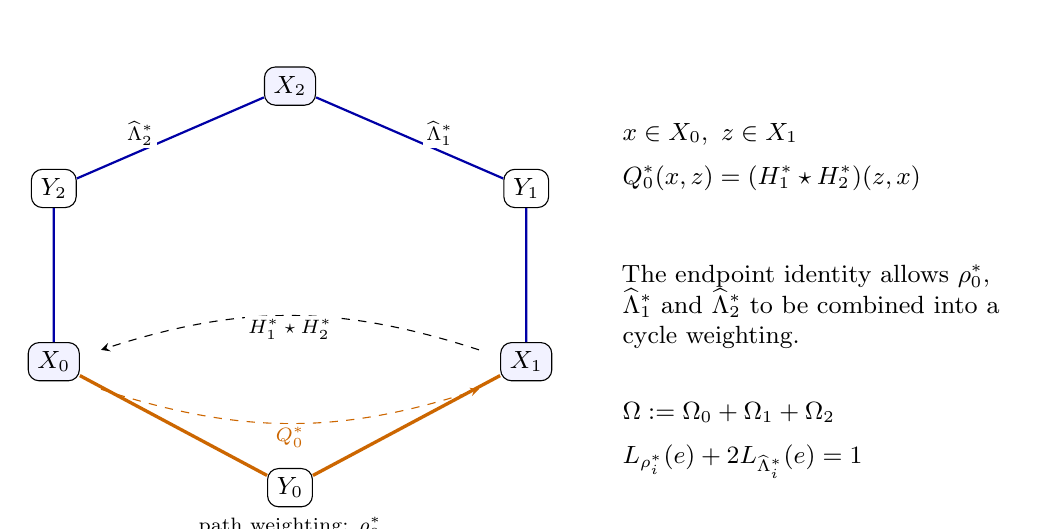
\begin{tikzpicture}[x=1cm,y=1cm,font=\small,>=stealth,
 dot/.style={circle,fill=black,inner sep=1.5pt},
 first/.style={blue!65!black,thick},
 second/.style={red!70!black,thick,dashed},
 shared/.style={green!35!black,very thick},
 spoke/.style={black!45,thin},
 tag/.style={fill=white,inner sep=1pt,font=\scriptsize}]

\node[draw,rounded corners,fill=blue!5] (X0) at (-3,0) {$X_0$};
\node[draw,rounded corners] (Y0) at (0,-1.6) {$Y_0$};
\node[draw,rounded corners,fill=blue!5] (X1) at (3,0) {$X_1$};
\node[draw,rounded corners] (Y1) at (3,2.2) {$Y_1$};
\node[draw,rounded corners,fill=blue!5] (X2) at (0,3.5) {$X_2$};
\node[draw,rounded corners] (Y2) at (-3,2.2) {$Y_2$};
\draw[very thick,orange!80!black] (X0)--(Y0)--(X1);
\draw[first] (X1)--(Y1)--(X2)--(Y2)--(X0);
\node[tag] at (0,-2.1) {path weighting: $\rho_0^*$};
\node[tag,align=center] at (1.9,2.9) {$\widehat\Lambda_1^*$};
\node[tag,align=center] at (-1.9,2.9) {$\widehat\Lambda_2^*$};
\draw[->,dashed] (2.4,.15) to[bend right=18]
 node[tag,below] {$H_1^*\star H_2^*$} (-2.4,.15);
\draw[->,dashed,orange!80!black] (-2.4,-.35) to[bend right=18]
 node[tag,below] {$Q_0^*$} (2.4,-.35);
\node[anchor=west,align=left] at (4.1,2.6)
 {$x\in X_0,\ z\in X_1$\\[5pt]
  $Q_0^*(x,z)=(H_1^*\star H_2^*)(z,x)$};
\node[anchor=west,align=left,text width=5.0cm] at (4.1,.7)
 {The endpoint identity allows $\rho_0^*$,
  $\widehat\Lambda_1^*$ and $\widehat\Lambda_2^*$ to be combined
  into a cycle weighting.};
\node[anchor=west,align=left] at (4.1,-1)
 {$\Omega:=\Omega_0+\Omega_1+\Omega_2$\\[5pt]
  $L_{\rho_i^*}(e)+2L_{\widehat\Lambda_i^*}(e)=1$};

\end{tikzpicture}
\caption{Combining path weightings for $k=3$ and $s=0$.
The solid segments schematically represent $G[X_i,Y_i]$ and
$G[Y_i,X_{i+1}]$, and the dashed arrows show the order of the
endpoint matrices. The identity
$Q_0^*=(H_1^*\star H_2^*)^{\mathsf T}$ allows the three path
weightings to be combined into a cycle weighting.
Summing over the three choices of $s$ uses each weighting $\rho_i^*$
once and each normalized residual weighting $\widehat\Lambda_i^*$ twice.}
\label{fig:cyclic:compatible-paths}
\end{figure}


For $\mathbf x\in\prod_iX_i$, define
\begin{equation*}
 J_s(\mathbf x):=
 \frac{\prod_{i\ne s}H_i^*(x_i,x_{i+1})}
      {\prod_{j\notin\{s,s+1\}}m_j(x_j)}.
\end{equation*}
This is the joint weighting in \eqref{doLpart:eq:chain-joint}
for the chain $X_{s+1},X_{s+2},\ldots,X_s$.
Its $(X_i,X_{i+1})$ marginal is $H_i^*$ for $i\ne s$,
and its $(X_{s+1},X_s)$ marginal is $K_s(\mathbf Q^*)$.
Since $\Phi(\mathbf Q^*)=\mathbf Q^*$, the definition of $\Phi_s$
gives $K_s(\mathbf Q^*)(z,x)=Q_s^*(x,z)$.
Thus the $(X_s,X_{s+1})$ marginal of $J_s$ is $Q_s^*$.
Lemma~\ref{doLpart:lem:conditional-realization}, applied to the
vertex-class sequences $(X_i,Y_i,X_{i+1})$ with mass $B=M/k$,
joint weighting $J_s$, and path weightings $\rho_s^*$ on
$\mathcal P_s$ and $\widehat\Lambda_i^*$ on $\mathcal P_i$
for $i\ne s$, gives $\Omega_s$ by
\eqref{doLpart:eq:conditional-cycle-weight}.

Let $\Omega:=\sum_{s=0}^{k-1}\Omega_s$. For each $P\in\mathcal P_i$,
the marginal identity in Lemma~\ref{doLpart:lem:conditional-realization} gives
\begin{equation*}
 \sum_{C:\,P_i(C)=P}\Omega(C)
 =\rho_i^*(P)+(k-1)\widehat\Lambda_i^*(P)
 =\rho_i^*(P)+\Lambda_i^{Q_i^*}(P).
\end{equation*}
Consequently, for every $e\in E(G_{{\rm path},i})$,
\begin{equation*}
 \sum_{C:\,e\in E(C)}\Omega(C)
 =L_{\rho_i^*}(e)+(k-1)L_{\widehat\Lambda_i^*}(e)=1.
\end{equation*}
The sets $E(G_{{\rm path},i})$ partition $E(G)$, so $\Omega$ is
a fractional part-respecting $C_{2k}$-decomposition of $G$.
\end{proof}

\subsection{Proof of Theorem~\ref{doLpart:thm:odd}}
\label{app:cyclic:odd}
\begin{proof}
Put $\delta:=\delta_{\rm cyc}(G)$, $X_i:=V_{2i}$ for $0\le i\le k$,
and $Y_i:=V_{2i+1}$ for $0\le i<k$.
The sets $E(G[X_i,Y_i])\cup E(G[Y_i,X_{i+1}])$ for $0\le i<k$,
together with $E(G[X_k,X_0])$, partition $E(G)$.
Local balance implies that each bipartite graph between
consecutive vertex classes has the same number $M$ of edges.
Let $m_i(x):=d_{\rm cyc}(x)/k$ for $x\in X_i$ and $B:=M/k$.
For $0\le i<k$, let $\calT_i$ be the set of nonnegative matrices on
$X_i\times X_{i+1}$ with row sums $m_i$ and column sums $m_{i+1}$.
This is a nonempty compact convex set, since it contains the matrix
with entries $m_i(x)m_{i+1}(z)/B$.

Fix $Q_i\in\calT_i$. For $x\in X_i$ and $z\in X_{i+1}$, put
$c_i(x,z):=|N_G(x;Y_i)\cap N_G(z;Y_i)|$.
Then $c_i(x,z)\ge d_{\rm cyc}(x)+d_{\rm cyc}(z)-n\ge2\delta-n>0$.
Let $\mathcal P_i$ be the two-edge paths $(x,y,z)$ in $G$ with
$x\in X_i$, $y\in Y_i$ and $z\in X_{i+1}$.
Define $\rho_i^{Q_i}(x,y,z):=Q_i(x,z)/c_i(x,z)$ on $\mathcal P_i$,
and extend it by zero to the other triples.
The identity $\sum_{y\in Y_i}\rho_i^{Q_i}(x,y,z)=Q_i(x,z)$
shows that $\rho_i^{Q_i}$ has endpoint matrix $Q_i$.
For $xy\in E_G(X_i,Y_i)$, its load is at most
$\frac{d_{\rm cyc}(x)/k}{d_{\rm cyc}(x)+\delta-n}\le1$, because
$(k-1)d_{\rm cyc}(x)+k\delta-kn\ge(2k-1)\delta-kn\ge0$.
The column sums of $Q_i$ give the corresponding bound on every
$yz\in E_G(Y_i,X_{i+1})$.

Define the residual capacities
\begin{equation*}
 A_i^{Q_i}(x,y):=\ind_{xy\in E(G)}-\sum_z\rho_i^{Q_i}(x,y,z),
 \qquad
 D_i^{Q_i}(y,z):=\ind_{yz\in E(G)}-\sum_x\rho_i^{Q_i}(x,y,z).
\end{equation*}
They are nonnegative and vanish on absent pairs.
For $y\in Y_i$, local balance gives
$d_G(y;X_i)=d_G(y;X_{i+1})$.
Subtracting $\sum_{x,z}\rho_i^{Q_i}(x,y,z)$ from both sides yields
$h_i^{Q_i}(y):=\sum_xA_i^{Q_i}(x,y)=\sum_zD_i^{Q_i}(y,z)$.
Set
\begin{equation*}
 \Lambda_i^{Q_i}(x,y,z):=
 \begin{cases}
 A_i^{Q_i}(x,y)D_i^{Q_i}(y,z)/h_i^{Q_i}(y),&h_i^{Q_i}(y)>0,\\
 0,&h_i^{Q_i}(y)=0.
 \end{cases}
\end{equation*}
Then $\sum_z\Lambda_i^{Q_i}(x,y,z)=A_i^{Q_i}(x,y)$ and
$\sum_x\Lambda_i^{Q_i}(x,y,z)=D_i^{Q_i}(y,z)$.
The bound $0\le\Lambda_i^{Q_i}(x,y,z)\le h_i^{Q_i}(y)$ proves
continuity in $Q_i$ also when the denominator vanishes.
The residual sums at $x\in X_i$ and $z\in X_{i+1}$ are
$(k-1)m_i(x)$ and $(k-1)m_{i+1}(z)$.
Thus the matrix
$H_i(Q_i)(x,z):=(k-1)^{-1}\sum_{y\in Y_i}\Lambda_i^{Q_i}(x,y,z)$
has row sums $m_i$ and column sums $m_{i+1}$.
It belongs to $\calT_i$ and depends continuously on $Q_i$.
The matrix $K(x_k,x_0):=k^{-1}\ind_{\{x_kx_0\in E(G)\}}$
has row sums $m_k$, column sums $m_0$ and mass $B$.

For $\mathbf Q=(Q_0,\ldots,Q_{k-1})\in\prod_i\calT_i$, define
\begin{equation*}
 \Phi_i(\mathbf Q):=
 \bigl(H_{i+1}(Q_{i+1})\star\cdots\star H_{k-1}(Q_{k-1})
 \star K\star H_0(Q_0)\star\cdots\star H_{i-1}(Q_{i-1})\bigr)^{\mathsf T},
\end{equation*}
omitting a string of $H_j$ matrices when its index range is empty.
Here, $\star$ is \eqref{doLpart:eq:composition}, with denominator
$m_j(x)$ at a vertex $x\in X_j$.
Before transposition, the displayed matrix has row sums $m_{i+1}$
on $X_{i+1}$ and column sums $m_i$ on $X_i$.
Thus $\Phi:=(\Phi_i)_{i=0}^{k-1}$ is a continuous self-map of
the nonempty compact convex set $\prod_i\calT_i$.
Brouwer's fixed-point theorem (Theorem~\ref{thm:prelim:brouwer})
therefore gives a fixed point $\mathbf Q^*$ of $\Phi$.
Write $\rho_i:=\rho_i^{Q_i^*}$, $\Lambda_i:=\Lambda_i^{Q_i^*}$
and $H_i:=H_i(Q_i^*)$.

Fix $s\in\{0,\ldots,k-1\}$.
The chain from $X_{s+1}$ to $X_s$ has successive matrices
$H_{s+1},\ldots,H_{k-1}$, $K$, and $H_0,\ldots,H_{s-1}$.
Equation~\eqref{doLpart:eq:chain-joint} gives their joint weighting
$J_s$ on $\prod_{j=0}^kX_j$, with mass $B$ and these consecutive
pair marginals. Its $(X_s,X_{s+1})$ marginal is
$\Phi_s(\mathbf Q^*)=Q_s^*$.
For $0\le i<k$, put
\begin{equation*}
 \lambda_i^{(s)}:=
 \begin{cases}\rho_i,&i=s,\\\Lambda_i/(k-1),&i\ne s,\end{cases}
 \qquad
 P_i^{(s)}:=
 \begin{cases}Q_i^*,&i=s,\\H_i,&i\ne s.\end{cases}
\end{equation*}
The endpoint matrix of $\lambda_i^{(s)}$ is $P_i^{(s)}$.
For a part-respecting cycle
$C=(x_0,y_0,x_1,y_1,\ldots,x_{k-1},y_{k-1},x_k)$, define
\begin{equation*}
 \Omega_s(C):=J_s(x_0,\ldots,x_k)
 \prod_{i=0}^{k-1}
 \frac{\lambda_i^{(s)}(x_i,y_i,x_{i+1})}
      {P_i^{(s)}(x_i,x_{i+1})}
\end{equation*}
when $J_s(x_0,\ldots,x_k)>0$, and set $\Omega_s(C):=0$ otherwise.
Every denominator in the first case is positive because
$P_i^{(s)}$ is a marginal of $J_s$.
Moreover, $J_s>0$ implies $x_kx_0\in E(G)$, since its
$(X_k,X_0)$ marginal is $K$.
For each $(x_0,\ldots,x_k)$ with $J_s(x_0,\ldots,x_k)>0$,
each quotient in the product sums to one over $y_i$.
The disjoint vertex classes ensure that all choices with positive
weight form part-respecting cycles.
Summing over the other $x_j$ and $y_j$ gives
\begin{equation*}
 \sum_{C:\,(x_i,y_i,x_{i+1})=(x,y,z)}\Omega_s(C)
       =\lambda_i^{(s)}(x,y,z),\qquad
 \sum_{C:\,x_k=x,\ x_0=z}\Omega_s(C)=K(x,z).
\end{equation*}
A zero endpoint marginal gives zero on both sides of the respective
identity, so these equalities hold for all specified paths and pairs.

Let $\omega:=\sum_{s=0}^{k-1}\Omega_s$.
Its weighting on the paths in $\mathcal P_i$ is
$\rho_i+(k-1)\Lambda_i/(k-1)=\rho_i+\Lambda_i$.
Consequently every edge of $G[X_i,Y_i]\cup G[Y_i,X_{i+1}]$
has load one.
Every edge $x_kx_0$ of $G[X_k,X_0]$ has load $kK(x_k,x_0)=1$.
Thus $\omega$ is a fractional part-respecting
$C_{2k+1}$-decomposition of $G$.
\end{proof}

\subsection{Sharpness of the threshold}

\begin{proposition}\label{doLpart:prop:sharp}
Let $\ell\ge3$ and $n\ge2$ be integers with $n$ even,
and let $t$ be an integer satisfying $0\le t<n/(2(\ell-1))$.
Then there is a locally balanced $\ell$-cyclic graph $G$ with classes
$V_0,\ldots,V_{\ell-1}$ of size $n$, such that $d_G(v;V_{i-1})=d_G(v;V_{i+1})=n/2+t$ for all $v\in V_i$, and $G$
has no fractional part-respecting $C_\ell$-decomposition.
\end{proposition}
\begin{proof}
For each $i\in\mathbb Z/\ell\mathbb Z$, let
$V_i=V_i^0\dot\cup V_i^1$ with $|V_i^0|=|V_i^1|=n/2$.
We choose $f_i\in\{0,1\}$ such that
\begin{equation}
\label{doLpart:eq:sharp-parity}
 \sum_{i=0}^{\ell-1} f_i=1\pmod2.
\end{equation}
For $b\in\{0,1\}$, the graph $G[V_i^b,V_{i+1}^{b+f_i}]$
is complete, whereas $G[V_i^b,V_{i+1}^{1+b+f_i}]$ is
$t$-regular, with superscripts read modulo two.
Such a $t$-regular bipartite graph exists by identifying both
parts with $\mathbb Z/(n/2)\mathbb Z$ and joining $x$ to $x+j$
for $0\le j<t$. The graph $G$ has no other edges.
Every vertex has cyclic degree $n/2+t$, and each graph between
consecutive classes has $M:=n(n/2+t)$ edges.
Let $D$ be the union of the edge sets of the $t$-regular
bipartite graphs. Then $|D|=\ell nt$.
We consider a part-respecting cycle $C=(v_0,\ldots,v_{\ell-1})$, and let $b_i\in\{0,1\}$ satisfy
$v_i\in V_i^{b_i}$. Define $\varepsilon_i:=b_i+b_{i+1}+f_i\pmod2$. Then $v_iv_{i+1}\in D$ exactly when
$\varepsilon_i=1$. Since each $b_i$ occurs twice in the sum, $\sum_i\varepsilon_i =\sum_i f_i =1\pmod2$ by
\eqref{doLpart:eq:sharp-parity}. Thus every part-respecting cycle contains at least one edge of $D$.

For any fractional packing $\omega$ of the part-respecting
$C_\ell$-copies in $G$, we have
\begin{equation*}
 \sum_C\omega(C)
 \le
 \sum_C |E(C)\cap D|\omega(C)
 =
 \sum_{e\in D}\sum_{C\ni e}\omega(C)
 \le |D|.
\end{equation*}
Since $M-|D|=n^2/2-(\ell-1)nt>0$, a fractional part-respecting
$C_\ell$-decomposition would satisfy
$\sum_C\omega(C)=e(G)/\ell=M>|D|$, a contradiction.
\end{proof}

For even $n$, let $t:=\left\lceil\frac{n}{2(\ell-1)}\right\rceil-1$. Then Proposition~\ref{doLpart:prop:sharp}
gives a counterexample of cyclic degree $\frac n2+t = \left\lceil\frac{\ell n}{2(\ell-1)}\right\rceil-1$.
Thus, for every even $\ell\ge4$, the degree bound in
Theorem~\ref{doLpart:thm:main} is sharp for each even $n$.
As $n$ ranges over the even integers, these examples also show
that the coefficient $\ell/[2(\ell-1)]$ cannot be decreased.


\section{Concentration and sampling estimates}

\subsection{Proof of Lemma~\ref{lem:pr:wi-interactions}}
\label{app:proof:lem-pr-wi-interactions}
\begin{proof}
Let $J_1\subseteq J$ consist of the coordinates on which at least
one indicator $I_f$ with $f\in E_1$ depends. Let $J_2\subseteq J\setminus J_1$
consist of the remaining coordinates on which at least one indicator
$I_f$ with $f\in E_2$ depends. Then
$|J_1|\le CBa$ and $|J_2|\le CBa^2$. Set
\begin{equation*}
 c_j:=\begin{cases}
 CB/a,&j\in J_1,\\
 CB/a^2,&j\in J_2,\\
 0,&j\notin J_1\cup J_2.
 \end{cases}
\end{equation*}
Recall that $b(f)=\sum_{T\ni f}w_T$ is the total weight of the
terms containing the indicator $I_f$.
For outcomes $\mathbf z,\mathbf z'$ differing only at coordinate $j$,
each product $\prod_{f\in T}I_f$ changes only if at least one of its
indicators changes, and its absolute change is at most one.
Since $w_T\ge0$, summing over $T\in\mathcal T$ gives
\begin{equation*}
 |Z(\mathbf z')-Z(\mathbf z)|
 \le\sum_{f:I_f(\mathbf z')\ne I_f(\mathbf z)}b(f).
\end{equation*}
At most $B$ indicators with $b(f)>0$ change. If $j\in J_1$, each
has $b(f)\le C/a$, since $a\ge1$. If $j\in J_2$, all such indicators
belong to $E_2$, so each has $b(f)\le C/a^2$. If $j\notin J_1\cup J_2$, no indicator with $b(f)>0$ changes.
Thus $|Z(\mathbf z')-Z(\mathbf z)|\le c_j$ in every case, and $\sum_{j\in J}c_j^2 \le CBa(CB/a)^2+CBa^2(CB/a^2)^2 \le 2C^3B^3/a$.

\end{proof}



\subsection{Proof of Theorem~\ref{thm:new:fresh-candidacy}}
\label{app:proof:thm-new-fresh-candidacy}
\begin{proof}
We choose $0<\eta_0\ll p_*,a,\epsilon,1$ and put
$\zeta_R:=\eta_0/10$, $\zeta_B:=\zeta_R/4$ and $\zeta:=\zeta_B$.
These choices precede $b,\rho$.
Recall that $m'=\lfloor\rho m\rfloor$, $n'=\lfloor\rho n\rfloor$
and $s_R=\min\{m',n'\}$.
We first prove the conclusion for independent uniform subsets of
sizes $m',n'$, allowing both part changes and edge deletions bounded
by $\zeta_Rs_R$. We then couple these subsets to the Bernoulli samples.

\paragraph{Fixed-size subsets.}
We choose $A_R\subseteq A$ and $B_R\subseteq B$ independently and
uniformly with sizes $m',n'$, respectively.
For every $x\in A$ and $y\in B$, the expectations of the degrees
into $B_R$ and $A_R$ are $(p\pm\eta_0)n'$ and $(p\pm\eta_0)m'$.
Recall that $J$ joins distinct $x,x'\in A$ precisely when
$|N_D(x)\cap N_D(x')|>(p^2+\eta_0)n$.
For every $x\in A$ and $x'\in A\setminus(N_J(x)\cup\{x\})$, the expected common-neighbor
count in $B_R$ is at most $(p^2+\eta_0)n'$.
Each count changes by at most one under a single exchange of the
sampled subset. The sampling concentration inequality
(Lemma~\ref{lem:simp:product-sampling}), with
deviation $\eta_0n'$ or $\eta_0m'$, therefore gives an event
$\mathcal E_R$ on which
\begin{equation}
\begin{gathered}
 d_D(x;B_R)=(p\pm2\eta_0)n'\quad(x\in A),\\
 d_D(y;A_R)=(p\pm2\eta_0)m'\quad(y\in B),\\
 |N_D(x)\cap N_D(x')\cap B_R|\le(p^2+2\eta_0)n'
                    \quad(x\in A,\ x'\in A\setminus(N_J(x)\cup\{x\})).
\end{gathered}
\label{eq:new:fresh-endpoint-candidacy:E5}
\end{equation}
There are at most $2N+N^2$ counts. For sufficiently large $N$,
$s_R\ge\rho aN/2$, so
\begin{equation}
 \Pr(\mathcal E_R^c)
 \le 8(N+1)^2\exp(-2\eta_0^2s_R)
 \le 8(N+1)^2\exp(-\eta_0^2\rho aN).
 \label{eq:prob:thm:new:fresh-candidacy}
\end{equation}
The estimates include vertices outside $A_R$ and $B_R$.

On $\mathcal E_R$, let $A''\subseteq A$, $B''\subseteq B$ and
$F\subseteq D[A'',B'']$ satisfy
$|A''\triangle A_R|+|B''\triangle B_R|\le\zeta_Rs_R$
and $\Delta(F)\le\zeta_Rs_R$, and put $D'':=D[A'',B'']-F$.
For $x\in A''$, $y\in B''$ and distinct $x,x'\in A''$,
\begin{equation*}
\begin{aligned}
 |d_{D''}(x)-d_D(x;B_R)|&\le2\zeta_Rs_R,\\
 |d_{D''}(y)-d_D(y;A_R)|&\le2\zeta_Rs_R,\\
 |N_{D''}(x)\cap N_{D''}(x')|
 &\le |N_D(x;B_R)\cap N_D(x';B_R)|+\zeta_Rs_R.
\end{aligned}
\end{equation*}
Also $||A''|-m'|,||B''|-n'|\le\zeta_Rs_R$.
Consequently $d_{D''}(x)=(p\pm5\eta_0)|B''|$ for $x\in A''$
and $d_{D''}(y)=(p\pm5\eta_0)|A''|$ for $y\in B''$.
By \eqref{eq:new:fresh-endpoint-candidacy:E5},
\begin{equation*}
 |N_{D''}(x)\cap N_{D''}(x')|\le(p^2+5\eta_0)|B''|
 \quad(x\in A'',\ x'\in A''\setminus(N_J(x)\cup\{x\})).
\end{equation*}
Thus $J[A'']$, of maximum degree at most $b$, contains every
pair exceeding this common-neighbor bound.

Since $p-5\eta_0\ge p_*/2$, the preceding degree estimates give
clause \textup{(i)}.
For $P\subseteq A''$ and $Q\subseteq B''$ with
$|P|\ge\epsilon|A''|$ and $|Q|\ge\epsilon|B''|$,
Lemma~\ref{lem:new:cuts-from-codegrees}, applied to $D''$
with exception graph $J[A'']$ and error $5\eta_0$, gives
\begin{equation*}
 \left|\frac{e_{D''}(P,Q)}{|P||Q|}-p\right|^2
 \le\frac{15\eta_0}{\epsilon}
       +\frac{b+1}{\epsilon^2|A''|}<\frac{p_*^2}{4}
\end{equation*}
for large $N$, since $|A''|\ge(1-\zeta_R)\rho aN/2$.
Thus $e_{D''}(P,Q)\ge(p-p_*/2)|P||Q|\ge(p_*/2)|P||Q|$.
These conclusions hold simultaneously on $\mathcal E_R$
for every $A'',B'',F$ satisfying the stated bounds
with allowance $\zeta_Rs_R$.

\paragraph{Bernoulli subsets.}
Let $A$ and $B$ have independent uniformly random orderings,
and independently let $K_A\sim\operatorname{Bin}(m,\rho)$
and $K_B\sim\operatorname{Bin}(n,\rho)$.
The first $m'$ and $n'$ entries define $A_R$ and $B_R$,
while the first $K_A$ and $K_B$ entries define independent
Bernoulli subsets $A_B$ and $B_B$.
For fixed $\rho$, Chernoff's inequality (Lemma~\ref{lem:prelim:chernoff}) gives an event
$\mathcal E_\Delta$ such that
$|A_B\triangle A_R|+|B_B\triangle B_R|\le\zeta_Rs_R/4$ and $\Pr(\mathcal E_\Delta^c)\le4e^{-c_\Delta N}$ for
some $c_\Delta>0$, independent of the graph and of $N$.
On $\mathcal E_R\cap\mathcal E_\Delta$, any $A''\subseteq A$,
$B''\subseteq B$ with $|A''\triangle A_B|+|B''\triangle B_B|
\le\zeta_Bs_R$ satisfy
\begin{equation*}
\begin{aligned}
 |A''\triangle A_R|+|B''\triangle B_R|
 &\le |A''\triangle A_B|+|B''\triangle B_B|
       +|A_B\triangle A_R|+|B_B\triangle B_R|\\
 &\le(\zeta_B+\zeta_R/4)s_R=\zeta_Rs_R/2.
\end{aligned}
\end{equation*}
Also every $F\subseteq D[A'',B'']$ with $\Delta(F)\le\zeta_Bs_R$
satisfies $\Delta(F)\le\zeta_Rs_R$. The fixed-size conclusion
therefore proves both clauses simultaneously for all these
$A'',B'',F$.
Let $\mathcal E_B$ be the event that the two clauses hold for all
changes to $A_B,B_B$ in their stated ranges. This event depends only
on $A_B,B_B$, and the coupling gives
\begin{equation}
 \Pr(\mathcal E_B^c)
 \le 8(N+1)^2e^{-\eta_0^2\rho aN}+4e^{-c_\Delta N}.
 \label{eq:prob:cor:new:bernoulli-candidacy}
\end{equation}
For sufficiently large $N_0$ in terms of $b,\rho$ and the
fixed parameters $p_*,a,\epsilon$, both failure bounds
\eqref{eq:prob:thm:new:fresh-candidacy} and
\eqref{eq:prob:cor:new:bernoulli-candidacy} are at most $N^{-10}$.
\end{proof}

\subsection{Proof of Lemma~\ref{lem:pr:marked-realisation}}
\label{app:proof:lem-pr-marked-realisation}
\begin{proof}
We use the independent variables defining the raw interval assignment
and the physical-edge variables $(C_e)_{e\in E(P)}$ from the statement.
Consider first $N_i:=N_V^{\rm mark}(A_i;\iota_i)$ from
\eqref{eq:cn:marked-row-count}, where $\iota_i$ specifies the sets
$(S_\tau^e,T_\tau^e)_{\tau,e},J_0,J_K$.
Recall that $A_i^\circ$ in
\eqref{eq:cn:admissible-outer-set}, with $A=A_i$ and pattern $\iota_i$,
consists of those $z\in A_i$ for which the prescribed physical arcs
$a_{\tau,e}(x,z)$, $x\in S_\tau^e$, belong to their permitted sets
$E_\tau$ and have pairwise distinct underlying undirected edges.
In the expansion of $N_i$ over this set, the required spokes
in each summand have distinct hubs.
The variables determining these spoke states are independent
across hubs and independent of the physical-edge variables.
Multiplying the required state probabilities therefore gives
the corresponding summand of $\mu_i$.
For $N_i:=N_U^{\rm mark}(B_i;S_0,S_K)$ from
\eqref{eq:cn:marked-index-count}, the labels in $S_0\cup S_K$
are $F$-independent. Their determining interval coordinates are
therefore disjoint. For each $u\in B_i$, the probability that all
required spokes are present is $s_0(u)^{|S_0|}s_K(u)^{|S_K|}$.
Summing over $u$ gives $\mathbb E N_i=\mu_i$.

Each summand depends on at most $K_{h,d}$ coordinates for a
constant $K_{h,d}\ge1$. One interval coordinate affects at most
$3d+1$ possible summation vertices.
For a physical edge $\{x,y\}$, the possible auxiliary arcs are
$(x\to y,0)$, $(y\to x,0)$,
$(x\to\pi^{-1}(y),K)$ and $(y\to\pi^{-1}(x),K)$.
Thus changing $C_{\{x,y\}}$ affects only a bounded number of summands. In $N_U^{\rm mark}(B_i;S_0,S_K)$, each coordinate
belongs to a single hub.
After increasing $K_{h,d}$, at most $K_{h,d}a_i$ independent
coordinates affect $N_i$, each with change bound at most $K_{h,d}$.
For $N_V^{\rm mark}$, we use $a_i:=|A_i|$ even when the summation
is restricted to $A_i^\circ$. For $N_U^{\rm mark}$, we use $a_i:=|B_i|$.
If $N_i$ is constant, it equals $\mu_i$. Otherwise McDiarmid's
bounded-differences inequality
(Theorem~\ref{thm:prelim:bounded-differences}) gives failure
probability at most $2\exp(-2\varepsilon^2a_i/K_{h,d}^3)$.
A union bound proves the assertion with $c_{h,d}:=2/K_{h,d}^3$.
\end{proof}



\subsection{Proof of Lemma~\ref{lem:completion:ordinary-reference-cuts}}
\label{app:proof:lem-completion-ordinary-reference-cuts}
\begin{proof}
Let $0<\eta\ll\alpha,\omega_*,p_*$, independently of $d$,
and put $L:=6d$, $B:=4d+3$.
We use \ref{item:ordinary-law:S1}--\ref{item:ordinary-law:S3}
for the ordinary completion sample.
For distinct $u,u'\in U$ and $v\in V$, the expectations of
$d_{H_0}(u)$, $|N_{H_0}(u)\cap N_{H_0}(u')|$
and $d_{H_0}(v)$ are $p_Hn$, $p_H^2n$ and $p_H|U|$,
respectively.
For the first two counts, \ref{item:ordinary-law:S1} and
\ref{item:ordinary-law:S3} give independent interval coordinates
with bounded influence. For the last count, the summands at
distinct hubs are independent. McDiarmid's bounded-differences
inequality (Theorem~\ref{thm:prelim:bounded-differences})
therefore applies to all three counts.
For $R_0^\to$, the comparison bipartite graph has parts
$V_{\rm out},V_{\rm in}$ and an edge $x_{\rm out}y_{\rm in}$
whenever $xy\in E(P^{\rm adm})$.
Each edge of this comparison graph belongs to $R_0^\to$ with
probability $p_R/2$. The in- and outdegrees of $\vec R_0$ have means
$(p_R/2)d_{P^{\rm adm}}(x)$.
For distinct $x,y$, the common out-neighbor count and
$|N^+_{\vec R_0}(x)\cap N_{P^{\rm adm}}(y)|$ have means
$(p_R/2)^2|N_{P^{\rm adm}}(x)\cap N_{P^{\rm adm}}(y)|$
and $(p_R/2)|N_{P^{\rm adm}}(x)\cap N_{P^{\rm adm}}(y)|$,
respectively, up to $O(1)$ endpoint exclusions.
Different physical edges have independent states.
McDiarmid's bounded-differences inequality
(Theorem~\ref{thm:prelim:bounded-differences}) gives failure at most
$2\exp(-a_{L,B}n)$ for each of the $O(n^2)$ degree and
common-neighborhood estimates with error $\eta n$. A union bound
therefore gives simultaneous failure at most $C_{L,B}n^2\exp(-a_{L,B}n)$.

For large $n$, $\delta(P^{\rm adm})\ge(1/2+\alpha/2)n$.
We use Corollary~\ref{cor:cn:relative-typicality-large-cuts} with
degree margin $\alpha_{\rm cut}=\alpha/2$, probability lower bound
$p_{\rm cut}=p_*/2$ and minimum-degree coefficient $\nu=p_*/8$.
For $H_0$, the parts are $(U,V)$ and we take $(G,J)=(K_{U,V},H_0)$
and $p=p_H$. For $R_0^\to$, we use the comparison graph just
defined and $p=p_R/2$.
The degree estimates give minimum degrees at least $\nu$ times
the opposite part size in both sampled graphs. We take
$0<\delta_c\le\min\{\alpha/8,p_*/64\}$.
The hierarchy gives
$\sqrt{12\eta/\nu+16/(\nu^2\omega_*n)} \le p_{\rm cut}\alpha_{\rm cut}/4$
for sufficiently large $n$. The preceding common-neighbor estimates
verify both inequalities in \eqref{eq:cn:relative-cut-input}, with
these parameters for all distinct vertices of the first part.
The corollary therefore supplies both cut conditions with coefficient
$h_0:=\tfrac12\min\{\nu,p_{\rm cut}\alpha_{\rm cut}\}$.
We take $2h\le h_0$. This proves
\eqref{eq:family:OF.C1}. The corollary gives every cut on the same
event, so the preceding failure bound proves
\eqref{eq:prob:lem:family:ordinary-cut-bounds}, with constants depending
only on $\alpha,\omega_*,p_*,d$. For sufficiently large $n_0$
in terms of these parameters, the failure probability is at most $n^{-10}$.
\end{proof}

\subsection{Proof of Lemma~\ref{lem:completion:marked-reference}}
\label{app:proof:lem-completion-marked-reference}
\begin{proof}
We choose additional constants such that
\begin{equation*}
 0<\delta_P\ll\xi
 \ll\varepsilon,\delta,\gamma,\kappa,k_*,t_*,\delta_D,h_D,\varrho_*,s_*,1/c.
\end{equation*}
The degree hypotheses give
$N/2\le D_0\le2N$.

\paragraph{Spoke degrees and intersections.}
Write $\mathcal B$ for the completion sample.
Its interval functions are $q_1(u)=t$ and $q_2(u)=a_u$.
We apply Lemma~\ref{lem:pr:marked-realisation} after relabeling
the pair states $\mathrm o_1,\mathrm o_2$ as $0,\bot$,
respectively, leaving the interval colors unchanged.
This gives $s_0(u)=s$ and leaves
$H^0_{\mathcal B},H^K_{\mathcal B}$ and the underlying variables
unchanged.

Let $F_{\pi,3d}$ join distinct vertices at $\pi$-distance at most
$3d$, so $\Delta(F_{\pi,3d})\le6d$.
For the physical-edge variables, we use
$E_j:=\mathscr E_j(P,\pi,3d)$ for $j\in\{0,K\}$ in
\eqref{eq:cn:distance-eligible-arcs} and $(p_0,p_K)=(p,k)$.
A state whose directed arc does not belong to $E_j$ for its
type $j$ is replaced by $\bot$.
This leaves the sampled rim graphs unchanged.
For each physical edge, the sum of the eligible state
probabilities is at most $2p+2k\le1$, and no eligible state
produces an auxiliary loop. This verifies the requirements in Lemma~\ref{lem:pr:marked-realisation}
for the physical-edge state probabilities and the absence of auxiliary loops.

For $j=0,K$, put $s_j:=s,t$, respectively. We apply
Lemma~\ref{lem:pr:marked-realisation} with $F=F_{\pi,3d}$,
$h=3$, $A=V$, $B=U$ and error $\xi$ to
\begin{equation*}
 \left|\bigcap_{\nu=1}^{q}N_{H^j_{\mathcal B}}(u_\nu)\right|
 \quad(q\in\{1,2,3\},\ u_1,\ldots,u_q\in U\text{ distinct}),
 \qquad d_{H^j_{\mathcal B}}(x)\quad(x\in V).
\end{equation*}
Their expectations are $s_j^qN$ and $s_jM$, respectively.
The resulting event depends only on the raw pair coordinates.
Fix $j\in\{0,K\}$ and distinct $x,y\in V$ with
$xy\notin E(F_{\pi,3d})$. By Lemma~\ref{lem:interval:raw-law},
the indicators
$\ind_{\{xu,yu\in E(H^j_{\mathcal B})\}}$, $u\in U$, are independent
Bernoulli variables with mean $s_j^2$. Hence
McDiarmid's bounded-differences inequality (Theorem~\ref{thm:prelim:bounded-differences}) gives
\begin{equation*}
 \Pr\left(
  \bigl||N_{H^j_{\mathcal B}}(x)\cap N_{H^j_{\mathcal B}}(y)|
       -s_j^2M\bigr|>\xi s_j^2M
 \right)
 \le2\exp(-2\xi^2s_j^4M).
\end{equation*}
A union bound over the two types and at most $N^2$ ordered
pairs gives failure probability at most
$4N^2\exp(-2\xi^2t_*^4\kappa N)$, since $s_j\ge t_*$
and $M\ge\kappa N$.
The exceptional sets $\{x\}\cup N_{F_{\pi,3d}}(x)$ have size at most
$6d+1$. Together with the preceding estimates, this gives failure
probability at most $C_dN^{K_{\rm prob}}\exp(-c_dN)$,
uniformly in $P$ and $(a_u,b_u)_{u\in U}$.

\paragraph{Rim degrees and cuts.}
For $j\in\{0,K\}$ and $e\in\{+,-\}$, the restriction
$\operatorname{dist}_\pi(v,z)>3d$ excludes at most $6d+1$ labels
$z$ from $M_j^e(v)$. Therefore the type-$0$ rim indegrees and outdegrees
have expectations $pD_0\pm p\delta_PN+O_d(1)$, and the type-$K$
expectations are $kD_0\pm k\delta_PN+O_d(1)$. The incoming type-$K$
expectation uses $d_P(\pi(v))$. Each degree is a sum over
distinct physical-edge coordinates.
For $p_0=p$ and $p_K=k$, the expected type-$j$ in- and
outdegrees are at least $p_j((1/2+\gamma)N-6d-1)$.
Hoeffding's inequality
(Theorem~\ref{thm:prelim:bounded-differences}), with deviation
$\min\{\varepsilon,\gamma k_*\}N/4$, gives error at most
$\varepsilon N/2$ about $p_jD_0$ and minimum in- and outdegrees
at least $p_jN/2$ for each type $j$, for sufficiently large $N$.

For $x\ne y$, at least $2\gamma N-O_d(1)$ labels in $N_P(x)\cap N_P(y)$
give eligible unmarked two-step paths. Each uses two distinct physical
edges, with probability $p^2$, and different middle labels use
disjoint physical coordinates. Chernoff's inequality (Lemma~\ref{lem:prelim:chernoff}) gives
$|N^+_{R^0_{\mathcal B}}(x)\cap N^-_{R^0_{\mathcal B}}(y)| \ge\tfrac32\gamma p^2N$ simultaneously for all
$x\ne y$.

Define bipartite graphs $J_0,J_K$ on $V_{\rm out},V_{\rm in}$ by
\begin{equation*}
 x_{\rm out}y_{\rm in}\in E(J_0)\iff(x,y)\in E_0,\qquad
 x_{\rm out}y_{\rm in}\in E(J_K)\iff(x,\pi(y))\in E_K.
\end{equation*}
Their minimum degrees are at least $(1/2+\gamma/2)N$ for large $N$.
For each $j\in\{0,K\}$ and all distinct $x,y\in V$, we apply
Lemma~\ref{lem:pr:marked-realisation}, with $F=F_{\pi,3d}$,
$h=2$, $A=V$ and error $\xi$, to
$|N_{R^j_{\mathcal B}}^+(x)\cap N_{R^j_{\mathcal B}}^+(y)|$
and $|N_{R^j_{\mathcal B}}^+(x)\cap M_j^+(y)|$.
The two outgoing arcs in a common-neighbor summand use
distinct physical edges. Replacing $M_j^+(y)$ in the mixed
intersection by $M_{j,\rm el}^+(y)$ removes at most
$6d+1\le\xi N$ vertices for sufficiently large $N$.
These estimates verify \eqref{eq:cn:relative-cut-input}
for $(G,J)=(J_j,D_{R^j_{\mathcal B}})$, probability $p_j$
and error $2\xi$, for all distinct vertices of the first part.

For each $j\in\{0,K\}$, we apply
Corollary~\ref{cor:cn:relative-typicality-large-cuts} with
$(G,J)=(J_j,D_{R^j_{\mathcal B}})$, $\alpha=\gamma/2$,
sampling probability and lower probability bound both equal to $p_j$,
and minimum-degree coefficient $\nu=p_j/2$. Since
$\sqrt{48\xi/k_*+64/(k_*^2N)}\le k_*\gamma/8$
by the hierarchy and $p_j\ge k_*$, the numerical condition holds
for both types. For $D_{R^j_{\mathcal B}}$, the coefficient in
\eqref{eq:cuts:large} is $\gamma p_j/4$.
For $D_{R^0_{\mathcal B}}$, the threshold may be taken as
$\min\{\gamma/64,p/128\}$; both $D_{R^0_{\mathcal B}}$ and
$D_{R^K_{\mathcal B}}$ satisfy the condition with threshold $\delta_D$.

For $H^j_{\mathcal B}$, we apply the same corollary with
$(G,J)=(K_{U,V},H^j_{\mathcal B})$, parts $(U,V)$
and probability $s_j$.
The preceding degree and common-neighbor estimates verify
\eqref{eq:cn:relative-cut-input}.
We use lower density $s_j$, $\alpha=1/4$ and
minimum-degree coefficient $s_j/2$.
The numerical condition follows from
$\sqrt{24\xi/t_*+64/(t_*^2M)}\le t_*/16$.
The corollary gives coefficient $s_j/8$ at threshold $\delta_D$.
Thus $D_{R^0_{\mathcal B}},D_{R^K_{\mathcal B}},
H^0_{\mathcal B},H^K_{\mathcal B}$ all have cut coefficient
at least $16h_D$.
The rim-degree, two-step and relative-count estimates fail
with probability at most $C_dN^{K_{\rm prob}}\exp(-c_dN)$.
On these estimates, the corollary gives every cut in the
large-cut condition. A union bound gives the asserted failure probability.
\end{proof}

\subsection{Proof of Lemma~\ref{lem:completion:marked-reference-configurations}}
\label{app:proof:lem-completion-marked-reference-configurations}
\begin{proof}
Put $k_*:=\varrho_*s_*/(2(c-1))$, $t_*:=s_*/(c-1)$ and
$a_{\rm cnt}:=\alpha t_*^2/8$. Before $d$ is specified, choose
\begin{equation*}
 0<\xi\ll\beta
 \ll a_{\rm cnt},\alpha,\kappa,k_*,t_*,s_*,1/c,\varrho_*.
\end{equation*}
Write $M:=|U|$, $p:=\varrho s/2$, $k:=p/(c-1)$, $t:=s/(c-1)$,
$s_0:=s$ and $s_K:=t$.
\paragraph{Compatible hubs and the two spoke classes.}
Let $\mathcal B$ be the marked completion sample in the statement. For each distinct
$u,u'\in U$, put $T_j:=N_{H^j_{\mathcal B}}(u)\cap N_{H^j_{\mathcal B}}(u')$ for $j\in\{0,K\}$. We apply
Lemma~\ref{lem:pr:marked-realisation} with $F$ joining distinct
labels at $\pi$-distance at most $3d$, $h=c$ and error $\xi$ to
$|T_j|$, $d_P(x;T_j)$ and $d_P(x;\pi(T_K))$ for all distinct $u,u'\in U$, all $x\in V$ and $j\in\{0,K\}$,
and to
$\widehat H_C(\mathcal B)$ for every $C\in\mathcal C_P$.
We use interval functions $q_1=t$, $q_2(u)=a_u$ and label-color functions
$\widetilde s_{\mathrm o_1}=s$, $\widetilde s_{\mathrm o_2}(u)=b_u$,
and selected colors $(g_0,j_0)=(1,\mathrm o_1)$.
For $|T_j|$, take $J_j=\{u,u'\}$ and all other sets empty
in \eqref{eq:cn:marked-row-count}. For $d_P(x;T_j)$, also take
$T_0^+=\{x\}$; for $d_P(x;\pi(T_K))$, take
$J_K=\{u,u'\}$ and $T_K^+=\{x\}$ instead, since
$d_P(x;\pi(T_K))=|T_K\cap\pi^{-1}(N_P(x))|$.
Each defining intersection contains at most three neighborhoods.
For $\widehat H_C(\mathcal B)$, the index count on $U$
requires type-$0$ spokes at the $c-1$ vertices of $V_0(C)$ and a
type-$K$ spoke at $y_C$. Their union $V(C)$ is $(3d,\pi)$-separated.
All these counts depend only on the pair variables of the original
raw experiment. Simultaneously for all the indicated roots, this gives $|T_j|=s_j^2N\pm \xi N$, $|T_j|\ge t_*^2N/2$, and \begin{equation*}
 d_P(x;T_j)\ge(1/2+\alpha/2)|T_j|\quad(j=0,K),\qquad d_P(x;\pi(T_K))\ge(1/2+\alpha/2)|T_K|\quad(x\in V).
\end{equation*}
Here $\mathbb E d_P(x;T_j)=s_j^2d_P(x)$ for $j\in\{0,K\}$,
and $\mathbb E d_P(x;\pi(T_K))=t^2d_P(x)$, since $s_K=t$
and $\pi$ is a bijection. The choice of $\xi$ gives the stated
minimum-degree bounds. In particular, any two vertices of $V$
have at least $\alpha|T_0|$ common neighbors in $T_0$ in $P$.
The classes $T_0,T_K$ are disjoint, and $T_0\cap\pi(T_K)=\varnothing$,
because $N_{H_{\mathcal B}^0}(u)$ lies outside
all successor-extended intervals assigned to $u$, whereas
$T_K\subseteq N_{H^K_{\mathcal B}}(u)$ lies in those intervals.

The estimate for $\widehat H_C(\mathcal B)$ gives
$\widehat H_C(\mathcal B)\ge M(ts^{c-1}-\xi)\ge32\beta N$
simultaneously for all $C\in\mathcal C_P$.
The probability that any of the preceding bounds on $|T_j|$,
$d_P(x;T_j)$, $d_P(x;\pi(T_K))$ or $\widehat H_C(\mathcal B)$ fails is
at most $C_dN^{K_{\rm prob}}\exp(-c_dN)$, with constants independent
of $P$ and $(a_u,b_u)_{u\in U}$.

\paragraph{Common cycles and paths.}
Condition on values of $(A_{u,a}),(G_{u,a}),(B_{u,x})$
for which the preceding neighborhood estimates hold.
For fixed distinct $u,u'\in U$, the sets $T_0,T_K$ are then
fixed, while $(C_e)_{e\in E(P)}$ remain independent with their
original distributions.
To count potential members of $\mathcal C(u,u')$, we choose
the marked head $x_0\in T_K$, then
$x_i\in N_P(x_{i-1})\cap T_0$ for $1\le i\le c-2$,
and finally $x_{c-1}\in
N_P(x_{c-2})\cap N_P(\pi(x_0))\cap T_0$.
For the pair $C_K(v,\mathbf z),C_K(v',\mathbf z)$ with $v\ne v'$,
the first and last labels satisfy
$z_1\in N_P(v)\cap N_P(v')\cap T_0$ and
$z_{c-1}\in N_P(\pi(v))\cap N_P(\pi(v'))\cap T_0$.
We choose $z_i\in N_P(z_{i-1})\cap T_0$ for $2\le i\le c-3$,
followed by $z_{c-2}\in N_P(z_{c-3})\cap N_P(z_{c-1})\cap T_0$.
For $C_0(v,\mathbf z),C_0(v',\mathbf z)$, both $z_1$ and $z_{c-1}$
lie in $N_P(v)\cap N_P(v')\cap T_0$.
The next labels satisfy $z_2\in N_P(z_1)\cap T_0$ and
$z_3\in\pi^{-1}(N_P(z_2))\cap T_K$.
The choices then proceed through $T_0$ as above, with $z_{c-2}$
in the common neighborhood of $z_{c-3},z_{c-1}$.
The marked arc is $z_2\to z_3$, with physical head $\pi(z_3)$.
These positions are distinct because $c\ge8$.

Each new label has $\pi$-distance greater than $3d$ from the
prescribed roots and all labels already chosen.
This excludes at most $(c+2)(6d+1)$ vertices at any choice.
For sufficiently large $N$, each choice has at least
$a_{\rm cnt}N$ possibilities.
There are therefore at least $a_{\rm cnt}^cN^c$ potential
common cycles and $a_{\rm cnt}^{c-1}N^{c-1}$ tuples $\mathbf z$
for each $j\in\{0,K\}$, with all required physical rim edges in $P$.
No separation is assumed between $v$ and $v'$,
and none of $vu,vu',v'u,v'u'$ is required to be present.

Every free label and its successor avoid the other free labels and
the roots. When $j=K$, the two closing physical edges have heads
$\pi(v),\pi(v')$. These heads may coincide with the opposite roots,
but neither can be a free label. The first and last free labels are
distinct, so no closing edge coincides with an opening edge. When
$j=0$, the common marked arc has physical head $\pi(z_3)$, different
from all rim labels of both cycles.
The unmarked edges are distinct, and shared path edges have identical
directions and types. Thus each tuple meets all physical conditions
of Definition~\ref{def:marked:common-paths}, using only the stated separation and $L_\pi>10d$.

\paragraph{Physical-edge exposure.}
We now expose $(C_e)_{e\in E(P)}$ under the preceding conditioning.
Each potential common cycle prescribes the states of $c$ distinct
physical rim edges. The union of $C_j(v,\mathbf z),C_j(v',\mathbf z)$
prescribes the states of at most $2c$ distinct physical rim edges.
Each prescribed state has probability at least $k_*$.
Conditional on the exposed pair variables, the expected values of
$|\mathcal C(u,u')|$ and $|\mathcal F_j(v,v';u,u')|$ are at least
$k_*^ca_{\rm cnt}^cN^c$ and
$k_*^{2c}a_{\rm cnt}^{c-1}N^{c-1}$, respectively.
For $|\mathcal C(u,u')|$, one physical-edge coordinate affects
$O_c(N^{c-2})$ tuples, since it fixes two rim labels.
The sum of the squared bounded-difference constants is
$O_c(N^{2c-2})$.
For $|\mathcal F_j(v,v';u,u')|$, at most $O(N)$ coordinates
meet $\{v,v',\pi(v),\pi(v')\}$, each affecting $O_c(N^{c-2})$ tuples.
Every other physical-edge coordinate affects $O_c(N^{c-3})$ tuples,
so the sum of the squared bounded-difference constants for
$|\mathcal F_j(v,v';u,u')|$ is $O_c(N^{2c-3})$.
By the choice of $\beta$, McDiarmid's bounded-differences inequality
(Theorem~\ref{thm:prelim:bounded-differences}) gives conditional
failure bounds $\exp(-c_{\rm cyc}N^2)$ and $\exp(-c_{\rm path}N)$
for the lower bounds $16\beta N^c$ and $16\beta N^{c-1}$.
A union bound over at most $N^2$ ordered hub pairs and
$2N^4$ choices of $(j,v,v',u,u')$, followed by averaging over
the conditioned pair variables, gives the asserted bounds
for $|\mathcal C(u,u')|$ and $|\mathcal F_j(v,v';u,u')|$.
The positive constants $c_{\rm cyc},c_{\rm path}$ are independent
of $d$. The failure probability for the preceding bounds on the
sets $T_0,T_K$ and on $\widehat H_C(\mathcal B)$ may depend on $d$;
adding it gives $C_dN^{K_{\rm prob}}e^{-c_dN}$.
\end{proof}

\subsection{Proof of Lemma~\ref{lem:list:raw}}
\label{app:proof:lem-list-raw}
\begin{proof}
For \eqref{eq:list:raw-bounds}, we prove failure probability at most
$C_{\rm list}n^3e^{-c_{\rm list}n}$, where the positive constants
depend only on $\alpha_{\rm list},p_{\rm list},s_{\rm list},d$.

Put $A:=V\setminus X$, and recall from Lemma~\ref{lem:list:raw} that
$E(H_0)=\{xw:B_{w,x}=0,\ x\notin\bigcup_{I\in\mathcal X_w^2}(I\cup\{I^+\})\}$.
For disjoint $R_+,R_-\subseteq V$ with $|R_+|+|R_-|\le2$
and $T=\{w\}\subseteq W$, we estimate the common neighborhood
$A\cap N_{H_0}(w)\cap\bigcap_{x\in R_+}N_{D_0}^+(x)
\cap\bigcap_{y\in R_-}N_{D_0}^-(y)$.
Let
\begin{equation*}
M_{\rm el}^\pm(x):=\{z\in N_G(x):\operatorname{dist}_\pi(x,z)>3d\},\qquad P_A:=A\cap\bigcap_{x\in R_+}M_{\rm
el}^+(x) \cap\bigcap_{y\in R_-}M_{\rm el}^-(y).
\end{equation*}
We apply Lemma~\ref{lem:pr:marked-realisation} with $h=3$,
$(G,W,V,W)$ playing the roles of $(P,U,X,Y)$, and
$F=(V,\{xy:x\ne y,\ \operatorname{dist}_\pi(x,y)\le3d\})$.
The raw interval sample has $q_1=0$, $q_2=q$ and $\mathcal J=\{0\}$.
We take $j_0=0$, $g_0=1$, $s_0=s$, $s_K=0$, $p_0=p$, $p_K=0$,
$E_0=\{(x,y):xy\in E(G),\ \operatorname{dist}_\pi(x,y)>3d\}$ and $E_K=\varnothing$. Projecting the
sampled directions outside $E_0$ to $\bot$ leaves
$D_0$ unchanged. Thus $(R^0,H^0)=(D_0,H_0)$ and $R^K=H^K=\varnothing$
in this application, with type $0$ assigned to these arcs and spokes.
The total probability of states on a physical edge is at most $2p\le1$.
For the row pattern, use $S_0^+=R_+$, $S_0^-=R_-$, $J_0=T$,
and empty sets for all other $S_\tau^e,T_\tau^e,J_K$.
Since $R_+\cap R_-=\varnothing$, the required undirected edges
at each $z\in P_A$ are distinct. Hence the summation set in
\eqref{eq:cn:admissible-outer-set} is exactly $P_A$.
With $\varepsilon=\alpha_{\rm list}p_{\rm list}^2s_{\rm list}/4$,
the lemma gives, simultaneously for these choices,
\begin{equation*}
\left|A\cap\bigcap_{x\in R_+}N_{D_0}^+(x) \cap\bigcap_{y\in R_-}N_{D_0}^-(y)\cap N_{H_0}(T)\right|=p^{|R_+|+|R_-|}\prod_{w\in T}s(w)|P_A|\pm \varepsilon |A|.
\end{equation*}
For the two-edge count, the fixed set $P_A$ has size at least
$2\alpha_{\rm list}n-|X|-(12d+2)\ge\alpha_{\rm list}n$
for large $n$. The one-edge and list counts have at least this many
labels in their respective sets $P_A$ and fewer required physical states. Every such raw
count is consequently at least
$3\alpha_{\rm list}p_{\rm list}^2s_{\rm list}n/4
=12\beta_{\rm list}n$.
There are at most a fixed multiple of $n^3$ counts, and
Lemma~\ref{lem:pr:marked-realisation} gives failure at most
$C_{\rm list}n^3\exp(-c_{\rm list}n)$ simultaneously.
For \eqref{eq:list:common-indices}, fix distinct $x,y\in V$.
For each $w\in W$, consider the event that every activation
with start in
$\bigcup_{z\in\{x,y\}}\{\pi^{-j}(z):0\le j\le d\}$
is zero and $B_{w,x}=B_{w,y}=0$.
This event implies $xw,yw\in E(H_0)$.
The activation condition has probability at least
$(1-a_d)^{2(d+1)}\ge e^{-3}$, where $a_d:=1/(2d+1)$.
Independently, the label-color condition has probability at least
$s_{\rm list}^2$, since
$s(w)/(1-(1+1/d)q(w))\ge s_{\rm list}$.
These events are independent across $w$, so the lower-tail
Chernoff bound (Lemma~\ref{lem:prelim:chernoff}) gives failure
probability at most $\exp(-e^{-3}s_{\rm list}^2|W|/8)$
for each pair.
The additional failure probability is thus at most
$n^2\exp(-e^{-3}s_{\rm list}^2|W|/8)$.
When $|W|\ge\kappa n$, its sum with the first failure bound
is at most $n^{-10}$ for sufficiently large $n$ in terms of
$\kappa$ and the preceding fixed parameters.
\end{proof}

\section{Matching, cuts and auxiliary constructions}

\subsection{Proof of Lemma~\ref{lem:new:weighted-resource-matching}}
\label{app:proof:lem-new-weighted-resource-matching}

\begin{theorem}[Carath\'eodory's theorem~{\cite[pp.~200--201]{Caratheodory1911}}]\label{thm:prelim:caratheodory}
Let $D$ be a nonnegative integer, let $X\subseteq\mathbb R^D$,
and let $z\in\operatorname{conv}(X)$.
Then there are $m\le D+1$ points $x_1,\ldots,x_m\in X$ and
$a_1,\ldots,a_m\ge0$ with $\sum_i a_i=1$ and $z=\sum_i a_ix_i$.
\end{theorem}

For simultaneous control of nonnegative functions on hyperedges,
we use the following simple-hypergraph theorem of Ehard, Glock
and Joos~\cite[Theorem~1.2]{EGJ2020}.

\begin{theorem}[Ehard--Glock--Joos]
\label{thm:prelim:weighted-matching}
Let $k\ge2$ be an integer, let $0<d<1$, and let $a:=d/(50k^2)$.
There is $\Delta_0=\Delta_0(k,d)$ such that the following holds for every $\Delta\ge\Delta_0$.
Let $\mathcal H$ be a simple $k$-uniform hypergraph with
$\Delta(\mathcal H)\le\Delta$, $\Delta_2(\mathcal H)\le\Delta^{1-d}$,
and $|E(\mathcal H)|\le\exp(\Delta^{a^2})$.
Let $\mathcal F$ be a family of at most $\exp(\Delta^{a^2})$
functions $f:E(\mathcal H)\to\mathbb R_{\ge0}$ satisfying
$f(E(\mathcal H))\ge\|f\|_\infty\Delta^{1+d}$.
Then there is a matching $M\subseteq E(\mathcal H)$ such that
\begin{equation*}
 f(M)=(1\pm\Delta^{-a})f(E(\mathcal H))/\Delta\qquad(f\in\mathcal F).
\end{equation*}
\end{theorem}

\begin{proof}[Proof of Lemma~\ref{lem:new:weighted-resource-matching}]
It suffices to consider $0<\gamma<1$. We choose
$0<\eta_0<\min\{1/10,\gamma/20\}$ and suppose
$V:=V(\mathcal H)\ne\varnothing$. The empty case is immediate.
Write $N:=|V|$, $\iota:=\iota_{\mathcal H}$ and $W:=\sum_h w(h)$.
Here $\iota(h)$ is the set of vertices incident with the edge index
$h$.
There is no bound on the number of parallel edge indices, so we
first reduce the support of $w$ to polynomially many edge indices
while preserving its total weight, weighted degrees, weighted
codegrees and the totals $W_g$.
For each $h\in E(\mathcal H)$ with $w(h)>0$, let
\begin{equation*}
 z_h:=\bigl((\mathbf1_{v\in\iota(h)})_{v\in V},
 (\mathbf1_{\{u,v\}\subseteq\iota(h)})_{\{u,v\}\in\binom V2},
 (g(h))_{g\in\mathcal F}\bigr).
\end{equation*}
Carath\'eodory's theorem (Theorem~\ref{thm:prelim:caratheodory}),
applied to $W^{-1}\sum_h w(h)z_h$, gives a weighting $w'$
supported on at most $3n^{2B}$ original edge indices, with
$d_{w'}(v)=d_w(v)$, $d_{w'}(u,v)=d_w(u,v)$,
$\sum_h w'(h)=W$ and $\sum_h g(h)w'(h)=W_g$ for every $g\in\mathcal F$.
Let $q:=2B+2$ and $T:=n^q$.
Replacing each supported edge $h$ by $\lfloor Tw'(h)\rfloor$
copies gives a multihypergraph with edge multiset $E$.
Each copy of $h$ retains the value $g(h)$ for every $g\in\mathcal F$.
For sufficiently large $n$,
\begin{equation*}
 (1-2\eta_0)T\le d(v)\le(1+\eta_0)T,\qquad
 d(u,v)\le TK/n,\qquad
 (1-\eta_0)TW_g\le g(E)\le TW_g.
\end{equation*}
Rounding decreases each degree by at most $3n^{2B}$ and gives
$0\le TW_g-g(E)\le3n^{2B}$ for every $g\in\mathcal F$.
Together with $W_g\ge an$, this gives the displayed bounds.

Let $k:=r+1$. Enlarging each copy of $h$ by
$k-|\iota(h)|$ new vertices, with disjoint new vertex sets for
distinct copies, gives a simple $k$-uniform hypergraph
$\widehat{\mathcal H}$.
We take $\Delta:=\lceil(1+\eta_0)T\rceil$ and $d_E:=1/(2q)$.
Its maximum degree is at most $\Delta$ and its maximum codegree is
at most $\max\{TK/n,1\}\le\Delta^{1-d_E}$ for large $n$.
On $E(\widehat{\mathcal H})$, we use the functions
$\widehat h\mapsto|\iota(h)\cap S|$ for $S\in\mathcal S$,
and $\widehat g(\widehat h):=g(h)$ for $g\in\mathcal F$,
where $h$ is the original edge index from which $\widehat h$ was obtained.
These functions have maximum at most $r$ and total at least
$aTn/2$. Their number is at most $2n^B$, and
$e(\widehat{\mathcal H})\le TW=O(n^{3B+2})$.
Since $\Delta^{1+d_E}=O(T\sqrt n)$, the mass and size conditions
of Theorem~\ref{thm:prelim:weighted-matching} hold for large $n$.

We apply the Ehard--Glock--Joos theorem
(Theorem~\ref{thm:prelim:weighted-matching}) to
$\widehat{\mathcal H}$ with these functions.
For sufficiently large $n$, its error
$\nu:=\Delta^{-d_E/(50k^2)}$ satisfies $\nu\le\eta_0$
and $\Delta\le(1+2\eta_0)T$.
Replacing each selected edge by its original edge index gives
a matching $M$ in $\mathcal H$: distinct selected copies have
disjoint original incidence sets, so each original edge is
selected at most once. Consequently
\begin{equation*}
 |S\cap V(M)|\ge
 \frac{(1-\nu)(1-2\eta_0)}{1+2\eta_0}|S|
 \ge(1-\gamma)|S|,
\end{equation*}
and
\begin{equation*}
 \frac{(1-\nu)(1-\eta_0)}{1+2\eta_0}W_g
 \le g(M)\le\frac{1+\nu}{1+\eta_0}W_g.
\end{equation*}
The choice of $\eta_0$ gives the required bounds for $g(M)$.
The order threshold may use common upper bounds on $r,B,K$
and positive lower bounds on $a,\gamma$.
The bound on the support of $w'$ makes the order threshold
independent of the number of parallel hyperedges in $\mathcal H$.
\end{proof}

\subsection{Proof of Lemma~\ref{lem:four:random-regularization}}
\label{app:proof:lem-four-random-regularization}
\begin{proof}
Put $\delta_0:=\min\{\beta/4,1/8\}$, $h:=\min\{\beta/2,1/4\}$ and $C:=4/h$.
We take $\eta_0>0$ sufficiently small in terms of $\beta$ and,
for each $0<\eta<\eta_0$, take $m_0\ge1/\eta$.
Write $s_0:=\sqrt\eta$ and $p:=Cs_0$.
The degree assumptions give
$d-s_0m\ge(1/2+\beta-\eta-s_0)m>0$, so $k\ge0$.
Put $f(v):=d_B(v)-k$ and
$M:=\sum_{v\in A_1}f(v)=\sum_{v\in A_2}f(v)$.
It suffices to choose a random spanning subgraph of $B$ with degrees
$f(v)$ and edge inclusion probabilities at most $p$, and remove it
from $B$.
The definition of $k$ and $m\ge1/\eta$ give $(s_0-\eta)m\le f(v)<(s_0+\eta)m+1 \le(s_0+2\eta)m$. The same bounds hold for $M/m$. Since
\begin{equation*}
 \frac{s_0+2\eta}{s_0-\eta}
   =1+\frac{3s_0}{1-s_0}\le1+\delta_0,
 \qquad \frac{s_0+2\eta}{p}
   =\frac{1+2s_0}{C}\le\frac h2,
\end{equation*}
we have $0<p<1$, $M/p\le hm^2/2$, and $\frac{f(v)}p\in(1\pm\delta_0)\frac{M}{pm}$ for all $v\in A_1\cup A_2$.

Let $S\subseteq A_1$ and $T\subseteq A_2$, and write
$s:=|S|/m$ and $t:=|T|/m$. Suppose $s+t>1-2\delta_0$.
If $s\le t$, then $t>1/2-\delta_0$ and $e_B(S,T)\ge |S|\bigl((1/2+\beta)m-(m-|T|)\bigr) \ge hm|S|$, since $\beta-\delta_0\ge h$.
The case $t\le s$ is symmetric. Thus
Lemma~\ref{lem:prelim:normalized-demands}, with both part sizes $m$,
$\delta=\delta_0$ and total demand $M/p$, gives
$q:E(B)\to[0,1]$ with incident sum $f(v)/p$ at every vertex $v$.
Set $z:=pq$. Then $z$ has incident sums $f(v)$ and
$0\le z(e)\le p$ for every $e\in E(B)$.

We show that every $x\in[0,1]^{E(B)}$ with incident sums $f(v)$
is a finite convex combination of indicators of spanning subgraphs
$D\subseteq B$ satisfying $d_D(v)=f(v)$ for every $v$.
We induct on the number of edges $e$ with $0<x(e)<1$.
If there are no such edges, $x$ itself is the indicator of such a
subgraph. Otherwise let $F_x$ be the spanning subgraph with edge set
$\{e\in E(B):0<x(e)<1\}$. For every vertex $v$,
\begin{equation*}
 \sum_{e\in E_{F_x}(v)}x(e)
   =f(v)-|\{e\in E_B(v):x(e)=1\}|\in\mathbb Z.
\end{equation*}
Thus $F_x$ has no vertex of degree one. A component of $F_x$
containing an edge has minimum degree at least two and hence
contains a cycle. Since $B$ is bipartite, this cycle has even
length. Write its edges in cyclic order as $e_1,\ldots,e_{2\ell}$,
and define $\sigma:E(B)\to\{-1,0,1\}$ by
\begin{equation*}
 \sigma(e_{2j-1}):=1,\quad \sigma(e_{2j}):=-1\quad(j\in[\ell]),
 \qquad \sigma(e):=0\quad(e\notin\{e_1,\ldots,e_{2\ell}\}).
\end{equation*}
Put
\begin{equation*}
 t_+:=\min_{j\in[\ell]}\{1-x(e_{2j-1}),x(e_{2j})\},\qquad
 t_-:=\min_{j\in[\ell]}\{x(e_{2j-1}),1-x(e_{2j})\},
\end{equation*}
and let $x^+:=x+t_+\sigma$ and $x^-:=x-t_-\sigma$.
Both $t_+$ and $t_-$ are positive. The vectors $x^+,x^-$ belong
to $[0,1]^{E(B)}$, and their incident sums remain $f(v)$ because
$\sigma$ has incident sum zero at each vertex. Each vector has
strictly fewer coordinates in $(0,1)$ than $x$. Moreover, $x=\frac{t_-}{t_++t_-}x^+ +\frac{t_+}{t_++t_-}x^-$.
Applying the induction hypothesis to $x^+$ and $x^-$ proves the claim.

In particular, write
$z=\sum_{i=1}^N\lambda_i\mathbf1_{E(D_i)}$, where $N\ge1$,
$\lambda_i\ge0$, $\sum_i\lambda_i=1$, and each $D_i\subseteq B$
is spanning with $d_{D_i}(v)=f(v)$ for every $v$.
We choose $i$ with probability $\lambda_i$ and let $R:=B-E(D_i)$.
Then $d_R(v)=d_B(v)-f(v)=k$ for every $v$, and
\begin{equation*}
 \Pr(e\notin E(R))
   =\sum_{i:e\in E(D_i)}\lambda_i=z(e)\le p=C\sqrt\eta
       \qquad(e\in E(B)).
\end{equation*}
\end{proof}



\subsection{Proof of Lemma~\ref{lem:new:cuts-from-codegrees}}
\label{app:proof:lem-new-cuts-from-codegrees}
\begin{proof}
Among the ordered pairs $(x,x')\in P\times P$, at most
$(b+1)|P|$ satisfy $x=x'$ or $xx'\in E(J)$. For these pairs
we use $|N_D(x)\cap N_D(x')|\le n$, and for all other pairs
we use the bound $(p^2+\eta)n$. Since $e_D(P,B)\ge(p-\eta)|P|n$ and $p\le1$,
\begin{equation*}
 \sum_{y\in B}(d_D(y;P)-p|P|)^2 =\sum_{x,x'\in P}|N_D(x)\cap N_D(x')| -2p|P|e_D(P,B)+p^2|P|^2n\le3\eta|P|^2n+(b+1)|P|n.
\end{equation*}
We apply Cauchy--Schwarz to
$e_D(P,Q)-p|P||Q|=\sum_{y\in Q}(d_D(y;P)-p|P|)$.
\end{proof}

\subsection{Proof of Lemma~\ref{lem:new:marked-endpoint-counts}}
\label{app:proof:lem-new-marked-endpoint-counts}
\begin{proof}
Recall from \eqref{eq:endpoints:index-table} that
$\overline P_{x,i}$ consists of potential arc occurrences,
$P_{x,i}$ consists of those present in $\mathcal Q$, and
$Q_{x,i}$ is the corresponding hub part. As in the statement,
$m_{x,i}=|\overline P_{x,i}|$.
The hypotheses imply $\kappa,p_*\le1$.
Put $\theta:=\varepsilon+\delta+(d+1)/a$ and $L:=6d+2$.
The definitions of $\overline P_{x,i}$ give
\begin{equation*}
 0\le d_P(\pi(x);A)-m_{x,1}\le L,\qquad
 0\le d_P(x;A)-m_{x,i}\le L\quad(i=2,3,4,5).
\end{equation*}
For incoming marked arcs the physical head is $\pi(x)$.
For outgoing marked arcs, $\pi(A)=A$ gives
$|A\cap\pi^{-1}(N_P(x))|=d_P(x;A)$.
The distance and loop exclusions remove at most $L$ possible endpoints.
Thus $m_{x,i}=D_A\pm (\delta a+L)$ and
$|P_{x,i}|=q_iD_A\pm 7\theta a$. We choose $C\ge1000(c+1)/(\kappa p_*)$.
If $e=C\theta\ge1$, the bounds follow from
$\mathcal N_{x,i}(a')\subseteq Q_{x,i}$,
$\mathcal M_{x,i}(u)\subseteq P_{x,i}$ and $0\le z_i\le1$.
We may therefore assume $e<1$.
Then $|P_{x,i}|\ge p_*a/4$ and
$|Q_{x,i}|\ge p_*b/2\ge\kappa p_*a/2$.
Using the estimates for $|\mathcal N_{x,i}(a')|$ and
$|Q_{x,i}|$ in \eqref{eq:endpoints:marked-input}, we obtain
\begin{equation*}
\bigl||\mathcal N_{x,i}(a')|-z_i|Q_{x,i}|\bigr| \le\bigl||\mathcal N_{x,i}(a')|-r_i z_i b\bigr|
+z_i\bigl||Q_{x,i}|-r_i b\bigr|\le2\varepsilon b\le(4\varepsilon/p_*)|Q_{x,i}|.
\end{equation*}
The estimates for $|\mathcal M_{x,i}(u)|$ and $|P_{x,i}|$ similarly give
\begin{equation*}
\bigl||\mathcal M_{x,i}(u)|-z_i|P_{x,i}|\bigr| \le\bigl||\mathcal M_{x,i}(u)|-z_iq_i m_{x,i}\bigr|
+z_i\bigl||P_{x,i}|-q_i m_{x,i}\bigr|\le2\varepsilon a\le(8\varepsilon/p_*)|P_{x,i}|.
\end{equation*}
For $a',a''\in\overline P_{x,i}$ with
$a''\notin\mathcal E_{x,i}(a')\cup\{a'\}$, the last inequality
of \eqref{eq:endpoints:marked-input} gives
$|\mathcal N_{x,i}(a')\cap\mathcal N_{x,i}(a'')| \le z_i^2|Q_{x,i}|+2\varepsilon b \le(z_i^2+4\varepsilon/p_*)|Q_{x,i}|$.
These inequalities prove \eqref{eq:endpoints:marked-counts}.

Let $a_0:=\kappa p_*/4$ and $e_0:=1/2$.
For $e\le e_0$, the preceding inequalities give
$|P_{x,i}|,|Q_{x,i}|\ge a_0a$.
Using $kD_A=tb$ and $s+t=ct$, we obtain
$k_x+l_x\le2tb+14\theta a$ and $s_x\ge ctb-2\varepsilon b$.
The choice of $C$ gives
$(14c+6)\theta a\le ctb$, since $tb\ge\kappa p_*a$.
Thus $c(k_x+l_x)\le3s_x$, proving
\eqref{eq:endpoints:marked-ratio}.
\end{proof}

\subsection{Proof of Lemma~\ref{lem:pr:ordinary-endpoints}}
\label{app:proof:lem-pr-ordinary-endpoints}
\begin{proof}
We partition $S$ uniformly into two sets $S_1,S_2$ of size $m$.
The hypergeometric Chernoff bound (Lemma~\ref{lem:prelim:chernoff})
combined with a union bound over $T$ shows that,
for sufficiently large $m$, there is a partition with
$d_D(u;S_i)\ge\lambda m/2$ for every $u\in T$ and $i\in\{1,2\}$.
We apply Lemma~\ref{lem:pairing:degree-cut-hall} to $D[S_1,T]$,
with $(s,\lambda,\epsilon)=(m,\lambda/2,\varepsilon)$, to obtain
a perfect matching. Write $v_u\in S_1$ for the vertex matched to $u$.

Let $D'$ be obtained from $D[S_2,T]$ by deleting, for each $u\in T$,
the edges from $u$ to $N_{B_0}(v_u)\cap S_2$.
At most $b_0$ edges are deleted at $u$.
At each $w\in S_2$, at most $b_0$ vertices $v_u$ are adjacent to $w$
in $B_0$, and these correspond to distinct vertices $u$.
Thus the deletion also has degree at most $b_0$ on $S_2$.
For sufficiently large $m$, we have $\delta(D')\ge\lambda m/4$.
For $X\subseteq S_2$, $Y\subseteq T$ with $|X|,|Y|\ge\varepsilon m$,
\begin{equation*}
 e_{D'}(X,Y)\ge\lambda|X||Y|-b_0\min\{|X|,|Y|\}>0,
\end{equation*}
since $\lambda\varepsilon m>b_0$.
Lemma~\ref{lem:pairing:degree-cut-hall}, applied to $D'$ with
$(s,\lambda,\epsilon)=(m,\lambda/4,\varepsilon)$, gives a perfect
matching. If $w_u\in S_2$ is matched to $u$, then
$uv_u,uw_u\in E(D)$ and $v_uw_u\notin E(B_0)$, as required.
\end{proof}

\subsection{Proof of Lemma~\ref{lem:completion:marked-local-extensions}}
\label{app:proof:lem-completion-marked-local-extensions}
\begin{proof}
We choose $0<\varepsilon_0\ll\alpha,\varrho_*,s_*,1/c$.
For each $d\ge2$, we take $a_0$ sufficiently large in terms of
$d$ and the constants in the preceding hierarchy.
Put $p_{\min}:=\varrho_*s_*/(2(c-1))$. The definitions of $p,k,s,t$
give $p_{\min}\le\min\{p,k,s,t\}$.
We first prove the bounds for $E_0,E_K,E_{00},E_{0K}$ in
\ref{item:extensions:marked-vertex}.
Recall from Section~\ref{sec:common:inner-extensions} that
$E_j(v,u;A)$ consists of labels $z\in A$ with
$v\to z\in E(R^j)$ and $zu\in E(H^j)$, where the physical
rim edge is loopless.
Membership in $E_{00}(v,w,u;A)$ requires
$v\to z,z\to w\in E(R^0)$ and $zu\in E(H^0)$.
For $E_{0K}(v,w,u;A)$, the second arc instead belongs to $R^K$,
while the spoke still belongs to $H^0$.
To apply \eqref{eq:extensions:marked-vertex-input}, we first bound
the following neighborhoods in $P$, before imposing the separation
restrictions that define $\overline R^0,\overline R^K$:
\begin{equation*}
\begin{array}{c|c}
 E_0(v,u;A)&A\cap N_P(v)\\
 E_K(v,u;A)&A\cap\pi^{-1}(N_P(v))\\
 E_{00}(v,w,u;A)&A\cap N_P(v)\cap N_P(w)\\
 E_{0K}(v,w,u;A)&A\cap N_P(v)\cap N_P(\pi(w)).
\end{array}
\end{equation*}
The first two sets in the right column have size at least
$(1/2+\alpha)a$, using $\pi(A)=A$ for the second.
The last two sets have size at least $2\alpha a$.
Since $P$ is simple, their defining neighborhoods already exclude
physical loops. The two physical edges are distinct when $v\ne w$
in $E_{00}$ and when $v\ne\pi(w)$ in $E_{0K}$.
To obtain the neighborhoods in $\overline R^0,\overline R^K$,
we exclude $z$ with $\operatorname{dist}_\pi(v,z)\le3d$ and,
in the last two rows, also $z$ with $\operatorname{dist}_\pi(z,w)\le3d$.
Each distance ball has at most $6d+1$ vertices, so the total loss
is at most $\ell:=12d+2$. We choose $a_0$ so that $\ell\le\alpha a/2$.

Replacing the neighborhoods of $P$ in the right column by the
corresponding neighborhoods of $\overline R^0,\overline R^K$
therefore leaves at least $(1/2+\alpha)a-\ell$ choices in the
first two rows and $2\alpha a-\ell$ choices in the last two rows.
The multipliers in \eqref{eq:extensions:marked-vertex-input}
are $ps,kt,p^2s,pks$, respectively, and each is at least
$p_{\min}^3$. By the choice of $\varepsilon_0$,
\begin{equation*}
\begin{aligned}
 |E_j(v,u;A)|
 &\ge p_{\min}^3((1/2+\alpha)a-\ell)-\varepsilon a
       \ge\alpha p_{\min}^3a/2 &&(j\in\{0,K\}),\\
 |E_{00}(v,w,u;A)|
 &\ge p_{\min}^3(2\alpha a-\ell)-\varepsilon a
       \ge\alpha p_{\min}^3a/2 &&(v\ne w),\\
 |E_{0K}(v,w,u;A)|
 &\ge p_{\min}^3(2\alpha a-\ell)-\varepsilon a
       \ge\alpha p_{\min}^3a/2 &&(v\ne\pi(w)).
\end{aligned}
\end{equation*}
For \ref{item:extensions:marked-index}, let $h:=|S_0|+|S_K|\le3$.
Equation~\eqref{eq:extensions:marked-index-input} gives
$|B\cap N_{H^0}(S_0)\cap N_{H^K}(S_K)|
\ge(p_{\min}^h-\varepsilon)b\ge p_{\min}^3b/2$
by the choice of $\varepsilon_0$.
We choose $\beta_*$ no larger than
$\min\{p_{\min}^3/2,\alpha p_{\min}^4/2\}$.
\end{proof}

\subsection{Proof of Lemma~\ref{lem:selection:bounded-fractional-matching}}
\label{app:proof:lem-selection-bounded-fractional-matching}
\begin{proof}
Let $B$ be the bipartite graph with parts $V_L:=\{v_L:v\in V(Q)\}$ and $V_R:=\{v_R:v\in V(Q)\}$, where $u_Lv_R\in E(B)$ if and only if $uv\in E(Q)$. Thus both parts have size $m$ and $\delta(B)\ge(1/2+\beta)m$.
Let $t:=\lfloor\beta m/2\rfloor$, so that $\beta m/4\le t\le\beta m/2$.
A greedy proper edge-coloring partitions $E(B)$ into at most $2m-1$ matchings.
We partition each nonempty color class into matchings of size at most $t$, obtaining an edge partition
$M_1,\ldots,M_K$. Since $e(B)\le m^2$, we have
$m/2 \le \Delta(B) \le K \le 2m-1+e(B)/t \le 5m/\beta$.

For each $i\in[K]$, define $a_i:=|M_i|$ and $B_i:=B-V(M_i)$. 
Both parts of $B_i$ have size $m-a_i$.
We choose $t$ pairwise edge-disjoint perfect matchings $N_{i,1},\ldots,N_{i,t}$ in $B_i$.
Indeed, after choosing the first $j-1$ matchings, where $j\in[t]$, the remaining graph has minimum degree at
least $(1/2+\beta)m-a_i-(j-1) \ge m/2 \ge (m-a_i)/2$. Hall's theorem (Theorem~\ref{thm:prelim:hall}) therefore supplies the next perfect
matching.
Thus $F_{i,j}:=M_i\cup N_{i,j}$ is a perfect matching of $B$
for every $i\in[K]$ and $j\in[t]$.
For $e\in E(B)$, let
$y(e):=(Kt)^{-1}\sum_{i=1}^K\sum_{j=1}^t
\mathbf1_{\{e\in F_{i,j}\}}$.
Then $\sum_{e\in E_B(z)}y(e)=1$ for every $z\in V(B)$.
Every edge $e$ belongs to exactly one $M_i$ and hence to all $t$ matchings $F_{i,1},\ldots,F_{i,t}$.
For each other index $i'$, it belongs to at most one $N_{i',j}$. Thus $1/K \le y(e)\le 1/K + 1/t$, and
consequently $\beta/(5m) \le y(e) \le 2/m + 4/(\beta m) \leq 5/(\beta m)$. For $uv\in E(Q)$, let
$\lambda(uv):=(y(u_Lv_R)+y(v_Lu_R))/2$.
The bounds on $y$ give the required bounds on $\lambda$.
Moreover, for every $v\in V(Q)$,
\begin{equation*}
 \sum_{u\in N_Q(v)}\lambda(uv)
 =
 \frac12\left(
 \sum_{u\in N_Q(v)}y(v_Lu_R)
 +
 \sum_{u\in N_Q(v)}y(u_Lv_R)
 \right)
 =1.
\end{equation*}
Hence $\lambda$ is a perfect fractional matching of $Q$.
\end{proof}

\subsection{Proof of Lemma~\ref{lem:new:marked-indegree-correction}}
\label{app:proof:lem-new-marked-indegree-correction}
\begin{proof}
Put $t_v:=|d_{M_0}^-(v)-f(v)|$ and set $E_v:=\varnothing$ when
$t_v=0$. For $t_v>0$, let $E_v$ consist of the incoming arcs in
$A\cap M_0$ if $d_{M_0}^-(v)>f(v)$, and in $A\setminus M_0$ otherwise.
Then $|E_v|\ge\rho n\ge t_v$ whenever $t_v>0$.
We seek a set $S\subseteq\bigcup_v E_v$ such that exactly $t_v$
arcs of $S$ enter each $v$, while at most
$\lceil\eta n/\rho\rceil$ arcs leave any vertex.
Let $B$ have a tail copy and a head copy of $V(P)$,
with an edge $u_Lv_R$ for each arc $u\to v$ in $E_v$.
Assigning weight $t_v/|E_v|$ to each edge $u_Lv_R$ of $B$ gives
weighted degree $t_v$ at $v_R$ and at most $\eta n/\rho$ at each tail.
The associated flow network has capacities
$\lceil\eta n/\rho\rceil$ from the source to each tail,
one from each tail to each adjacent head, and $t_v$
from head $v_R$ to the sink.
These weights extend to a feasible flow of value $\sum_vt_v$,
the total capacity into the sink.
Since all capacities are integral,
the max-flow/min-cut theorem (Theorem~\ref{thm:prelim:max-flow-min-cut}) gives an integral flow
of the same value.
Let $S\subseteq A$ be its selected arcs and put $M:=M_0\triangle S$.
Exactly $t_v$ selected arcs enter $v$, and at most
$\lceil\eta n/\rho\rceil$ leave each vertex.
By the definition of $E_v$, we have $d_M^-(v)=f(v)$ for every $v$
and $M\triangle M_0\subseteq A$.
Since the directions are fixed and $P$ is oriented, the underlying
change graph has maximum degree at most
$\eta n+\lceil\eta n/\rho\rceil \le(1+1/\rho)\eta n+1 \le(1+2/\rho)\eta n+n^{3/5}$,
proving \eqref{eq:new:orientation-and-types:O2}.
\end{proof}

\subsection{Proof of Lemma~\ref{lem:pr:wheel-codegrees-deletion}}
\label{app:proof:lem-pr-wheel-codegrees-deletion}
\begin{proof}
For a physical rim edge $e=\{x,y\}$, let
$X_e:=\{x,y,\pi^{-1}(x),\pi^{-1}(y)\}$.
For a spoke $e=vw$, with $v\in V$ and $w\in U$, let $X_e:=\{v\}$.
These sets contain every possible auxiliary rim endpoint
of an occurrence of $e$.
At most $2|X_e|\Delta(F)$ edges of $F$ meet $X_e\cup\pi(X_e)$.
For each such edge $f\ne e$, the sum of coefficients of candidates
containing $e,f$ is $O(1/n)$ by Lemma~\ref{lem:pr:wheel-codegrees}.
For every other $f\in E(F)$, each auxiliary representation of $f$
has both endpoints outside $X_e$. Prescribing this representation
therefore fixes two additional entries of the candidate tuple, giving
a coefficient sum of $O(1/n^2)$.
Only indices $i\in\mathcal I(e,a)$ with
$(E_V(i)\setminus\{e\})\cap E(F)\ne\varnothing$
can contribute to $Z_{e,a}-Z^F_{e,a}$.
Since $e(F)\le n\Delta(F)/2$, the total coefficient of these
indices is at most $C_Lu$. Every indicator in the defining products
lies in $[0,1]$, so $0\le Z_{e,a}-Z^F_{e,a}\le C_Lu$.
The products defining $Z_{e,a}$ and $Z^F_{e,a}$ omit the indicator
$\ind_{\{\sigma(e)=a\}}$, so the bound holds for every
$a\in\Sigma_e^{\rm app}$, regardless of $\sigma(e)$
and whether $e\in E(F)$.

For $T_{r,w}$, the hub $w$ is fixed.
Prescribing a physical rim edge and its position and direction
fixes two rim labels, so the total coefficient of candidates
containing that edge is $O(1/n)$.
Summing over $E(F)$ gives $C_Tun$.
All constants depend only on $\mathcal L$ and the coefficient bounds.
\end{proof}

\section{Proof of Theorem~\ref{thm:four:cycle-fractional-threshold}}
\label{app:proof:thm-four-cycle-fractional-threshold}
\begin{proof}
By Proposition~\ref{prop:four:lower}, $\delta_{C_r}\ge1/2$.
Put $q:=\delta_{C_r}$ and $h:=r$.
If $q=1$, the assertion is immediate, so suppose that $q<1$.
Fix $\varepsilon>0$. It is enough to consider $\varepsilon<1-q$.  Let $G$ be a sufficiently large $n$-vertex
graph with $\delta(G)\ge(q+\varepsilon)n$.
We shall partition $E(G)$ into edge sets $J_i$ of small maximum degree so that each $G-J_i$
is $C_r$-divisible and admits a $C_r$-decomposition. Averaging these
decompositions will give a fractional $C_r$-decomposition of $G$.
We choose a fixed integer $R$ such that $R\equiv1\pmod{2h}$ and $(q+\varepsilon)/R < \varepsilon/4$. We choose $0<\xi<\min\{\varepsilon/4,1/(4R)\}$.
\startlocalclaims
\begin{localclaim}\label{clm:threshold:divisible-partition}
For all sufficiently large $n$, there is a partition $E(G)=J_1\mathbin{\dot\cup}\cdots\mathbin{\dot\cup}J_R$ such that, for every $i\in[R]$ and $v\in V(G)$,
\begin{align}
 d_{J_i}(v)&\equiv d_G(v)\pmod2, \label{eq:four:2reg-parity}\\
 |J_i|&\equiv e(G)\pmod h, \label{eq:four:2reg-size}\\
 d_{J_i}(v)&\le \frac{d_G(v)}R+\xi n. \label{eq:four:2reg-degree}
\end{align}
\end{localclaim}
\begin{proof}
Let each edge of $G$ receive a color from $[R]$ independently
and uniformly, and let $J_i^0$ be the set of edges of color $i$.
Chernoff's bound (Lemma~\ref{lem:prelim:chernoff}) gives,
with probability tending to one,
$d_{J_i^0}(v)=d_G(v)/R\pm\xi n/4$
for all $v \in V(G)$ and $i \in [R]$.
For distinct $u,v$ and $i<R$, let $W_i^0(u,v)$ be the set of
vertices $w\in N_G(u)\cap N_G(v)$ for which the two edges $uw,vw$
have colors $i$ and $R$ in some order. Since $|N_G(u)\cap N_G(v)| \ge d_G(u)+d_G(v)-n \ge 2\varepsilon n$,
we have $\mathbb E|W_i^0(u,v)|\ge 4\varepsilon n / R^2$.
Another application of Chernoff's bound (Lemma~\ref{lem:prelim:chernoff}) and a union bound over the $O_R(n^2)$
choices show that we have
$|W_i^0(u,v)| \geq 2 \varepsilon n / R^2$ for all $u \ne v$ and $i < R$ simultaneously. Fix such a coloring.

Let $M:=e(G)$. For every $i<R$, choose
$a_i\in\{0,\ldots,h-1\}$ such that $|J_i^0|+a_i\equiv M\pmod h$.
The degree estimate above implies that $J_R^0$ has
$\Omega(n^2)$ edges, so we may recolor
$\sum_{i<R}a_i=O_{r,R}(1)$ distinct edges from color $R$ to
color $i$, using exactly $a_i$ edges for color $i$.
Let $J_i$ be the color classes after this recoloring.
Then $|J_i|\equiv M\pmod h$ for $i<R$.
Since $R\equiv1\pmod h$ and the color classes partition $E(G)$,
the same congruence holds for $i=R$.
For all sufficiently large $n$, the degree estimates have changed
by only $O_{r,R}(1)$, and every set $W_i^0(u,v)$ has lost only
$O_{r,R}(1)$ vertices. Hence, letting $\rho := \varepsilon/R^2$, we may assume that after the recoloring there are at least $\rho n$ choices of $w$ for every $u\ne v$ and $i<R$ such that $uw,vw$ have colors $i,R$ in some order.

It remains to correct the degree parities without changing
any color-class size.
For each $i<R$, let
$T_i:=\{v:d_{J_i}(v)\not\equiv d_G(v)\pmod2\}$.
Each $T_i$ has even cardinality, so it has a partition into pairs.
There are at most $(R-1)n/2$ resulting indexed pairs $(\{u,v\},i)$.
We choose a fixed integer $L$ with $(R-1)/(2L)<\rho/4$
and process these pairs successively.
For $(\{u,v\},i)$, we choose a path $uwv$ whose edges have colors
$i,R$ in some order, neither edge has been used in an earlier switch,
and $w$ has been used as the middle vertex of fewer than $L$ chosen paths.
Before the switching stage, there are at least $\rho n$ candidates satisfying the color condition. At any stage, fewer than $(R-1)n/(2L) < \rho n / 4$ vertices have already been used as middle vertices $L$ times.
Moreover, each vertex is an endpoint of at most one indexed pair
per color $i<R$ and is used as a middle vertex at most $L$ times.
Thus at most $R-1+2L$ previously used edges are incident with
each of $u,v$, excluding at most $2(R-1+2L)$ further candidates.
Since each switch changes only the colors of its two edges,
every remaining candidate still satisfies the color condition.
Hence the number of admissible choices is at least $\rho n-\frac{\rho n}{4}-2(R-1+2L)>0$ for sufficiently large $n$.

Interchanging the colors $i,R$ on each chosen path $uwv$
is well defined because these paths are edge-disjoint.
Each switch reverses the parity of $d_{J_i}(u)$ and $d_{J_i}(v)$,
leaves $d_{J_i}(w)$ unchanged, and preserves every color-class size.
After all switches, $d_{J_i}(v)\equiv d_G(v)\pmod2$ for all $v \in V(G)$ and $i < R$.
Since $R$ is odd and the color classes partition $E(G)$, the same
congruence follows for color $R$.  For $i<R$, the switching stage
changes the color-$i$ degree of any vertex by at most $1$; for
color $R$ it changes it by at most $R-1$.  Enlarging $n$ if
necessary, the claimed degree bound
\eqref{eq:four:2reg-degree} therefore holds.
\end{proof}

We take the partition from Claim~\ref{clm:threshold:divisible-partition}. For $i\in[R]$, let $H_i:=G-J_i$. Since every vertex of $C_r$ has degree two,~\eqref{eq:four:2reg-parity} and~\eqref{eq:four:2reg-size} show that each $H_i$ is $C_r$-divisible. Moreover,
\begin{align*}
    d_{H_i}(v) \ge (1-1/R)d_G(v)-\xi n \ge \left(q+\varepsilon-\frac{q+\varepsilon}{R}-\xi\right)n > (q+\varepsilon/2)n \ge (\delta_{C_r}+\varepsilon/2)n.
\end{align*}
Thus, for sufficiently large $n$, the definition of $\delta_{C_r}$
gives a $C_r$-decomposition $\mathcal D_i$ of every $H_i$.
Every edge of $G$ belongs to exactly $R-1$ of the graphs
$H_1,\ldots,H_R$. For each copy $C'$ of $C_r$ in $G$, define
$\omega(C'):=\frac1{R-1} \bigl|\{i\in[R]:C'\in\mathcal D_i\}\bigr|$. For every edge
$e\in E(G)$, $\sum_{C'\ni e}\omega(C') =\frac1{R-1}\bigl|\{i:e\in E(H_i)\}\bigr|=1$. Hence $\omega$ is a
fractional $C_r$-decomposition of $G$.
Since $\varepsilon>0$ was arbitrary, $\delta_{C_r}^*\le\delta_{C_r}$, as required.
\end{proof}


% BEGIN GLOSSARY
\clearpage
\section*{Glossary of definitions and notation}

Page numbers indicate where the terms and notation are defined.

\begingroup
\small
\setstretch{1.04}
\renewcommand{\arraystretch}{1.12}
\setlength{\LTpre}{.5\baselineskip}
\setlength{\LTpost}{.5\baselineskip}
\begin{longtable}{@{}>{\raggedright\arraybackslash}p{.50\textwidth}>{\raggedright\arraybackslash}p{.38\textwidth}r@{}}
\toprule
\textbf{Term} & \textbf{Notation or description} & \textbf{Page}\\
\midrule
\endfirsthead
\multicolumn{3}{@{}l}{\emph{Glossary of definitions and notation (continued)}}\\[.4ex]
\toprule
\textbf{Term} & \textbf{Notation or description} & \textbf{Page}\\
\midrule
\endhead
\bottomrule
\endfoot
% O03
\textbf{Additive error notation} & $a\pm b$ & \pageref{gls:interval-error-notation}\\
\addlinespace[.35ex]
% G44
\textbf{Auxiliary and physical incidence degrees} & $d_{\rm aux},d_{\rm phys},\Delta_*$ & \pageref{gls:auxiliary-and-physical-incidence-degrees}\\*
\hspace*{1em}Typed symmetric difference & $\mathcal Q\triangle\mathcal Q^{\prime}$ & \pageref{gls:auxiliary-and-physical-incidence-degrees:difference}\\
\addlinespace[.35ex]
% G26
\textbf{Bipartite representation of a digraph} & $D_R,\beta_R$ & \pageref{gls:bipartite-representation-of-a-digraph}\\
\addlinespace[.35ex]
% O07
\textbf{Candidate wheel indices and physical edge sets} & $i,E_V(i),E_U(i),\iota(i)$ & \pageref{gls:candidate-wheel-indices-and-physical-incidence-sets}\\
\addlinespace[.35ex]
% G70
\textbf{Common marked cycle estimates} & for one hub pair & \pageref{gls:common-marked-cycle-estimates}\\*
\hspace*{1em}Estimates for all hub pairs &  & \pageref{gls:common-marked-cycle-estimates:all-pairs}\\
\addlinespace[.35ex]
% G61
\textbf{Common ordinary cycle weights and absorber counts} & $T_{u,u^{\prime}},\mathcal C_{u,u^{\prime}},\phi_{u,u^{\prime}}$ & \pageref{gls:common-ordinary-cycle-weights-and-absorber-counts}\\
\addlinespace[.35ex]
% G51
\textbf{Common-path families at two hubs} & $C_j(v,\mathbf z)$; $\mathcal F_j(v,v^{\prime};u,u^{\prime})$ & \pageref{gls:common-path-families-for-marked-cycles-two-hubs}\\
\addlinespace[.35ex]
% G69
\textbf{Common spoke neighborhoods and selected subsets} & $A_0,B_0,K_v,O_v$ & \pageref{gls:common-typed-neighborhoods-and-restricted-cycle-path-families}\\*
\hspace*{1em}Potential vertex loads & $Z_{v,j}(\mathcal Q;\kappa,\phi)$ & \pageref{gls:common-typed-neighborhoods-and-restricted-cycle-path-families:loads}\\*
\hspace*{1em}Restricted common-cycle and common-path families & $\mathcal C_{\mathcal Q}(u,u^{\prime};A,B)$; $\mathcal F_j^{A,B}(v,v^{\prime};u,u^{\prime})$ & \pageref{gls:common-typed-neighborhoods-and-restricted-cycle-path-families:families}\\
\addlinespace[.35ex]
% G50
\textbf{Compatible hubs of marked cycles} & $\mathcal C_R,W_C$ & \pageref{gls:compatible-hubs-and-common-marked-cycles}\\*
\hspace*{1em}Common marked cycles at two hubs & $\mathcal C(u,u^{\prime})$ & \pageref{gls:compatible-hubs-and-common-marked-cycles:common-cycles}\\
\addlinespace[.35ex]
% O14
\textbf{Complement of a prescribed factor} & after reserving cycles or paths & \pageref{gls:complement-of-a-prescribed-factor}\\
\addlinespace[.35ex]
% G34
\textbf{Composition of endpoint matrices} & $K_{i-1}\star K_i$ & \pageref{gls:composition-of-endpoint-matrices}\\
\addlinespace[.35ex]
% G03
\textbf{Cycle divisibility} & $C_r$-divisible & \pageref{gls:cycle-divisibility}\\
\addlinespace[.35ex]
% G55
\textbf{Cycle-factor absorber templates} & $T=(\kappa_T,\mathcal M_0^T,\mathcal M_1^T)$ & \pageref{gls:cycle-factor-absorber-templates}\\
\addlinespace[.35ex]
% G58
\textbf{Cycle weight and absorber estimates} &  & \pageref{gls:cycle-weight-and-absorber-estimates}\\*
\hspace*{1em}Estimates with paired absorbers &  & \pageref{gls:cycle-weight-and-absorber-estimates:paired}\\
\addlinespace[.35ex]
% G30
\textbf{Cyclic-partite graphs} & $\ell$-cyclic graphs &
\pageref{gls:cyclic-partite-graph-and-interface}\\
\addlinespace[.35ex]
% G04
\textbf{Degree threshold for a set of allowed cycle lengths} & $\delta_{\mathcal S}=\sup_{r\in\mathcal S}\delta_{C_r}$ & \pageref{gls:threshold-for-a-set-of-cycle-lengths}\\
\addlinespace[.35ex]
% G02
\textbf{Degree threshold for cycle decompositions} & $\delta_{C_r}$ & \pageref{gls:cycle-decomposition-threshold}\\
\addlinespace[.35ex]
% G06
\textbf{Degree threshold for fractional cycle decompositions} & $\delta^*_{C_r}$ & \pageref{gls:fractional-cycle-decomposition-threshold}\\
\addlinespace[.35ex]
% O18
\textbf{Degree threshold for fractional triangle decompositions in tripartite graphs} & $\widehat\delta^*_{K_3}$; locally balanced graphs with equal parts & \pageref{gls:partite-fractional-triangle-threshold}\\
\addlinespace[.35ex]
% G05
\textbf{Degree threshold for resolvable cycle decompositions} & $\delta^{\rm res}_{C_r}$; regular graphs & \pageref{gls:resolvable-cycle-decomposition-threshold}\\
\addlinespace[.35ex]
% O02
\textbf{Explicit values of cycle-decomposition degree thresholds} & $\tau_r$ & \pageref{gls:explicit-cycle-threshold-constants}\\
\addlinespace[.35ex]
% G08
\textbf{Extended graphs (ordinary/untyped)} & $\mathcal G=(V,U,G,H)$ & \pageref{gls:extended-graph-ordinary-untyped}\\
\addlinespace[.35ex]
% G09
\textbf{Extended subgraphs (ordinary)} & $\mathcal G^{\prime}\subseteq\mathcal G$ & \pageref{gls:extended-subgraph-and-induced-restriction-ordinary}\\*
\hspace*{1em}Induced restrictions & $\mathcal G[S]$ & \pageref{gls:extended-subgraph-and-induced-restriction-ordinary:induced}\\
\addlinespace[.35ex]
% G77
\textbf{Extending lists} & $\lambda$-extending in $D$ & \pageref{gls:extending-lists}\\
\addlinespace[.35ex]
% G28
\textbf{Fractional graph decompositions} & $\mathcal C_F(G)$; $\omega$ & \pageref{gls:fractional-decomposition-with-capacities}\\*
\hspace*{1em}Decompositions with edge capacities & $a:E(G)\to\mathbb R_{\ge0}$ & \pageref{gls:fractional-decomposition-with-capacities:capacities}\\
\addlinespace[.35ex]
% G01
\textbf{Graph decompositions} & $F$-decomposition & \pageref{gls:cycle-decomposition-and-resolvability}\\*
\hspace*{1em}Resolvable decompositions &  & \pageref{gls:cycle-decomposition-and-resolvability:resolvable}\\*
\hspace*{1em}Packings and factors &  & \pageref{gls:cycle-decomposition-and-resolvability:packings-factors}\\
\addlinespace[.35ex]
% G07
\textbf{Hierarchy of constants} & $\ll$ & \pageref{gls:hierarchy-of-constants}\\
\addlinespace[.35ex]
% G78
\textbf{Indexed wheel hypergraph for preparation} & $\mathcal H(\sigma)$ & \pageref{gls:indexed-wheel-hypergraph-for-preparation}\\*
\hspace*{1em}Deletion of rim-edge vertices & $\mathcal H_F$ & \pageref{gls:indexed-wheel-hypergraph-for-preparation:deleted}\\
\addlinespace[.35ex]
% G76
\textbf{Interval assignments and their spoke graphs} & $(\mathcal I_w),(S_w)$;\newline $Y_w,B_w,Z_w,H^0,H^K$ & \pageref{gls:interval-assignments-and-their-spoke-graphs}\\
\addlinespace[.35ex]
% G56
\textbf{Labeled embeddings of absorber templates} & $\mathcal A_{\mathcal C}^{\mathcal T}(X)$ & \pageref{gls:labeled-embeddings-of-absorber-templates}\\*
\hspace*{1em}Labeled and rooted embedding convention &  & \pageref{gls:labeled-embeddings-of-absorber-templates:embedding-convention}\\*
\hspace*{1em}Ordered roots for one-class templates &  & \pageref{gls:labeled-embeddings-of-absorber-templates:ordered-roots}\\
\addlinespace[.35ex]
% G29
\textbf{Large-cut condition} & $(\delta,h)$ & \pageref{gls:large-cut-condition}\\
\addlinespace[.35ex]
% G31
\textbf{Local balance and cyclic degree} & $d_{\rm cyc},\delta_{\rm cyc}$ & \pageref{gls:local-balance-and-cyclic-degree}\\
\addlinespace[.35ex]
% G75
\textbf{Marked completion estimates} & $(\mathrm M1)$--$(\mathrm M5)$ & \pageref{gls:marked-completion-estimates}\\
\addlinespace[.35ex]
% G39
\textbf{Marked completion host} & $\mathcal Q$ & \pageref{gls:marked-completion-host}\\*
\hspace*{1em}Allowed typed arcs and spokes & $\mathfrak E^{\rm mark}$ & \pageref{gls:marked-completion-host}\\
\addlinespace[.35ex]
% G41
\textbf{Marked completion sample} & $\mathcal B=(R^0,R^K,H^0,H^K)$ & \pageref{gls:marked-completion-sample}\\
\addlinespace[.35ex]
% G63 + O10
\textbf{Marked endpoint assignment graphs} & $D_{x,i}$ & \pageref{gls:marked-endpoint-assignment-graphs}\\*
\hspace*{1em}Potential assignment graphs & $\overline D_{x,i}$ & \pageref{gls:marked-endpoint-assignment-graphs:potential}\\*
\hspace*{1em}Enlarged neighborhoods & $\mathcal N_{x,i},\mathcal M_{x,i}$ & \pageref{gls:marked-endpoint-assignment-graphs:neighborhoods}\\*
\hspace*{1em}Potential rim digraphs & $\overline R^0,\overline R^K$ & \pageref{gls:marked-endpoint-assignment-graphs:potential-rims}\\
\addlinespace[.35ex]
% G52
\textbf{Marked host estimates} & $(\mathrm{MH}1)$--$(\mathrm{MH}3)$ & \pageref{gls:marked-host-estimates}\\
\addlinespace[.35ex]
% G74
\textbf{Marked local cycle estimates} & on $(A,B;X,Y)$ & \pageref{gls:marked-local-cycle-estimates}\\
\addlinespace[.35ex]
% G65
\textbf{Marked local cycle families and potential vertex loads} & $\mathcal C_P^A$ & \pageref{gls:marked-local-cycle-families-and-potential-vertex-loads}\\*
\hspace*{1em}Potential vertex loads & $\widehat Z^A_{v,u,j}$ & \pageref{gls:marked-local-cycle-families-and-potential-vertex-loads:vertex-loads}\\*
\hspace*{1em}Cycles at one hub in the typed graph & $\mathcal C^A(u)$ & \pageref{gls:marked-local-cycle-families-and-potential-vertex-loads:actual-cycles}\\
\addlinespace[.35ex]
% G68
\textbf{Marked wheel absorbers} & marked $c$-wheel absorber for $L$ & \pageref{gls:marked-wheel-absorbers}\\
\addlinespace[.35ex]
% G43
\textbf{Marked wheel divisibility} & marked $c$-wheel-divisibility & \pageref{gls:marked-wheel-divisibility}\\
\addlinespace[.35ex]
% G21
\textbf{Marked wheels} & $\mathcal W_c^K(\mathcal Q)$ & \pageref{gls:marked-wheels}\\
\addlinespace[.35ex]
% G25
\textbf{Minimum cycle length of a permutation} & $L_\pi$ & \pageref{gls:shortest-permutation-cycle-and-separation-graph}\\*
\hspace*{1em}Separation graph & $F_{\pi,b}$ & \pageref{gls:shortest-permutation-cycle-and-separation-graph:separation-graph}\\
\addlinespace[.35ex]
% G27
\textbf{Multihypergraphs and incidence maps} & $\mathcal H,\iota_{\mathcal H}$ & \pageref{gls:indexed-hypergraphs-and-incidence-map}\\
\addlinespace[.35ex]
% G67
\textbf{One- and two-edge extension sets} & $E_j,E_{00},E_{0K}$ & \pageref{gls:one-and-two-edge-extension-sets}\\
\addlinespace[.35ex]
% G62
\textbf{One-hub marked cycle and common-path families} & $\mathcal C_w$ & \pageref{gls:one-hub-marked-cycle-and-common-path-families}\\*
\hspace*{1em}Common-path tuples at one hub & $\mathcal F_j(v,v^{\prime};w)$ & \pageref{gls:one-hub-marked-cycle-and-common-path-families:paths}\\*
\hspace*{1em}Restriction of the free labels to $A$ & $\mathcal F_j^A(v,v^{\prime};u)$ & \pageref{gls:one-hub-marked-cycle-and-common-path-families:restricted}\\
\addlinespace[.35ex]
% O15
\textbf{Ordinary and long classes of factors} & classes of prescribed factors & \pageref{gls:ordinary-and-long-classes-of-factors}\\
\addlinespace[.35ex]
% G73
\textbf{Ordinary completion estimates} & $(\mathrm O1)$--$(\mathrm O5)$ & \pageref{gls:ordinary-completion-estimates}\\
\addlinespace[.35ex]
% G38
\textbf{Ordinary completion host} & $\mathcal Q$ & \pageref{gls:ordinary-completion-host}\\*
\hspace*{1em}Allowed edges & $\mathfrak E^{\rm ord}$ & \pageref{gls:ordinary-completion-host}\\
\addlinespace[.35ex]
% G40
\textbf{Ordinary completion sample} & $\mathcal B=(R,H_{\rm ord})$ & \pageref{gls:ordinary-completion-sample}\\
\addlinespace[.35ex]
% G72
\textbf{Ordinary local cycle estimates} & on $(A,B;X,Y)$ & \pageref{gls:ordinary-local-cycle-estimates}\\
\addlinespace[.35ex]
% G64
\textbf{Ordinary local cycle families and potential vertex loads} & $\mathcal C_{P,F},\mathcal C_J,T_J$;\newline $\phi_J,\ell_v$ & \pageref{gls:ordinary-local-cycle-families-and-potential-vertex-loads}\\*
\hspace*{1em}Potential vertex loads & $Z_{v,J}$ & \pageref{gls:ordinary-local-cycle-families-and-potential-vertex-loads:vertex-loads}\\
\addlinespace[.35ex]
% G46
\textbf{Ordinary rim and spoke load operators} & $\mathcal L_R,\mathcal L_H$ & \pageref{gls:ordinary-rim-and-spoke-load-operators}\\
\addlinespace[.35ex]
% G59
\textbf{Ordinary wheel absorbers} & $r$-wheel absorber for $L$ & \pageref{gls:ordinary-wheel-absorbers}\\
\addlinespace[.35ex]
% G12
\textbf{Ordinary wheel divisibility} & $r$-wheel-divisible; divisible at $x$ & \pageref{gls:ordinary-wheel-divisibility}\\
\addlinespace[.35ex]
% G11
\textbf{Ordinary wheel packings and decompositions} & $\mathcal W_r^{\rm ord}(\mathcal G)$ & \pageref{gls:ordinary-wheel-packings-and-decompositions}\\*
\hspace*{1em}Fractional wheel decompositions &  & \pageref{gls:ordinary-wheel-packings-and-decompositions:fractional}\\
\addlinespace[.35ex]
% G60
\textbf{Ordinary wheel transformers} & $r$-wheel transformer & \pageref{gls:ordinary-wheel-transformers}\\
\addlinespace[.35ex]
% G57
\textbf{Paired cycle-factor absorbers} & $\mathcal A_{\mathcal C}^{\rm pair}(X)$ & \pageref{gls:paired-cycle-factor-absorbers}\\*
\hspace*{1em}Two-class restriction & $\mathcal A_{\mathcal C}(X)$ & \pageref{gls:paired-cycle-factor-absorbers:two-class}\\
\addlinespace[.35ex]
% O08
\textbf{Part-preserving edge-bijective homomorphism} & $\phi:L\to L^{\prime}$ & \pageref{gls:part-preserving-edge-bijective-homomorphism}\\
\addlinespace[.35ex]
% G32
\textbf{Part-respecting cycles} & $\mathcal C_\ell^{\rm part}(G)$ & \pageref{gls:part-respecting-cycles}\\*
\hspace*{1em}Fractional part-respecting decompositions &  & \pageref{gls:part-respecting-cycles:fractional}\\
\addlinespace[.35ex]
% G33
\textbf{Path weightings and endpoint matrices} & $G_{\rm path}$ &
\pageref{gls:path-weighting-edge-load-and-endpoint-matrix}\\*
\hspace*{1em}Path weightings & $\lambda$ & \pageref{gls:path-weighting-edge-load-and-endpoint-matrix:weighting}\\*
\hspace*{1em}Edge loads & $L_\lambda$ & \pageref{gls:path-weighting-edge-load-and-endpoint-matrix:edge-load}\\*
\hspace*{1em}Endpoint matrices & $K_\lambda$ & \pageref{gls:path-weighting-edge-load-and-endpoint-matrix:endpoint-matrix}\\*
\hspace*{1em}Weighted balance at the middle part &  & \pageref{gls:path-weighting-edge-load-and-endpoint-matrix:weighted-balance}\\
\addlinespace[.35ex]
% G24
\textbf{Permutation distance and separation} & $\operatorname{dist}_\pi$; $(b,\pi)$-separated & \pageref{gls:permutation-distance-and-separation}\\
\addlinespace[.35ex]
% O06
\textbf{Physical arcs with separated auxiliary endpoints} & $\mathscr E_0(P,\pi,b),\mathscr E_K(P,\pi,b)$ & \pageref{gls:directed-physical-arcs-allowed-by-separation}\\
\addlinespace[.35ex]
% G18
\textbf{Physical edge sets} & $E_{\rm phys}(\mathcal Q),E_R(\mathcal Q),E_H(\mathcal Q)$ & \pageref{gls:physical-edge-sets}\\
\addlinespace[.35ex]
% G16
\textbf{Physical image map} & $\operatorname{phys}$ & \pageref{gls:physical-image}\\
\addlinespace[.35ex]
% G17
\textbf{Physical injectivity} &  & \pageref{gls:physical-injectivity}\\
\addlinespace[.35ex]
% G54
\textbf{Potential compatible-hub count} & $\widehat H_C$ & \pageref{gls:potential-compatible-hub-count}\\
\addlinespace[.35ex]
% G53
\textbf{Potential marked wheel loads} & $\mathfrak E_P,\mathcal W_P,\widehat L_e$ & \pageref{gls:potential-marked-wheel-loads}\\
\addlinespace[.35ex]
% G49
\textbf{Potential ordinary wheel loads and configuration counts} & $\widehat L_e$ & \pageref{gls:potential-ordinary-wheel-loads-and-configuration-counts}\\*
\hspace*{1em}Potential rim-configuration counts & $\widehat I_e$ & \pageref{gls:potential-ordinary-wheel-loads-and-configuration-counts:rim-count}\\*
\hspace*{1em}Potential transfer counts & $\widehat T_{v,u,u^{\prime}}$ & \pageref{gls:potential-ordinary-wheel-loads-and-configuration-counts:transfer-count}\\
\addlinespace[.35ex]
% O17
\textbf{Preparation: potential loads and wheel-weight sums} & $Z^F_{e,a},Z_{e,a}$ & \pageref{gls:preparation-potential-loads-and-hub-totals}\\*
\hspace*{1em}Total weight of unmarked $r$-wheels at $w$ & $T^F_{r,w},T_{r,w}$ & \pageref{gls:preparation-potential-loads-and-hub-totals:hub-totals}\\
\addlinespace[.35ex]
% G36
\textbf{Raw interval sample} & $(\mathcal X_w^g),(B_{w,x})$ & \pageref{gls:raw-interval-sample}\\
\addlinespace[.35ex]
% G42
\textbf{Restricted balance differences} & $b^{A,B}$ (ordinary) & \pageref{gls:restricted-balance-differences}\\*
\hspace*{1em}Marked restricted differences & $a^{+,A,B},a^{-,A,B}$;\newline $a^{K,A,B},a^{U,A}$ & \pageref{gls:restricted-balance-differences:marked}\\*
\hspace*{1em}Unrestricted marked differences & $a^+,a^-,a^K,a^W$ & \pageref{gls:restricted-balance-differences:unrestricted}\\*
\hspace*{1em}Restricted balance norm & $\|\mathbf a^{A,B}\|_{X,Y}$ & \pageref{gls:restricted-balance-differences:norm}\\
\addlinespace[.35ex]
% G47
\textbf{Rim-load correction configurations} & $\mathcal S(e,u)$ & \pageref{gls:rim-load-correction-configurations}\\*
\hspace*{1em}Vertex sets defined from $P$ and $\mathcal F$ & $\mathcal S_P(e)$ & \pageref{gls:rim-load-correction-configurations:parent}\\
\addlinespace[.35ex]
% G23
\textbf{Separated wheel families} & $\mathcal W(\mathcal G;b,\pi)$ & \pageref{gls:separated-wheel-families}\\
\addlinespace[.35ex]
% G37
\textbf{Spoke-color assignment from intervals} & $\sigma_{\mathcal Z}$; $\sigma_{\mathcal X}$ & \pageref{gls:spoke-color-assignment-from-intervals}\\
\addlinespace[.35ex]
% G48
\textbf{Spoke-load transfer configurations} & $\mathcal T(v,u,u^{\prime})$ & \pageref{gls:spoke-load-transfer-configurations}\\*
\hspace*{1em}Configurations in $(P-E(\mathcal F),V\times U)$ & $\mathcal T_P(v;u,u^{\prime})$ & \pageref{gls:spoke-load-transfer-configurations:parent}\\
\addlinespace[.35ex]
% G45
\textbf{Stars of vertex and hub sets} & $\operatorname{star}(A,B)$ & \pageref{gls:star-of-a-vertex-hub-pair}\\
\addlinespace[.35ex]
% G35
\textbf{Successor intervals} & $I$ & \pageref{gls:successor-intervals-and-extended-disjointness}\\*
\hspace*{1em}Terminal successor and extended interval & $I^+,\widehat I$ & \pageref{gls:successor-intervals-and-extended-disjointness:extended}\\*
\hspace*{1em}Successor-extended disjointness &  & \pageref{gls:successor-intervals-and-extended-disjointness:disjointness}\\
\addlinespace[.35ex]
% G66
\textbf{Triangle endpoint families and loads} & $\mathcal T_x$ & \pageref{gls:triangle-endpoint-families-and-loads}\\*
\hspace*{1em}Potential endpoint loads & $Z_{x,v},Z_{x,u}$ & \pageref{gls:triangle-endpoint-families-and-loads:endpoint-loads}\\
\addlinespace[.35ex]
% G14
\textbf{Typed extended graph} & $\mathcal Q=(R^0,R^K,H^0,H^K)$ & \pageref{gls:typed-extended-graph}\\
\addlinespace[.35ex]
% G15
\textbf{Typed extended subgraph and restriction} & $\mathcal Q^{\prime}\subseteq\mathcal Q$; $\mathcal Q[A\cup B]$ & \pageref{gls:typed-extended-subgraph-and-restriction}\\
\addlinespace[.35ex]
% G22
\textbf{Typed wheel packings and decompositions} & unmarked and marked & \pageref{gls:typed-wheel-packings-and-decompositions}\\*
\hspace*{1em}Fractional typed wheel decompositions &  & \pageref{gls:typed-wheel-packings-and-decompositions:fractional}\\
\addlinespace[.35ex]
% G19
\textbf{Unmarked and marked directed cycles} & $C$ & \pageref{gls:unmarked-and-marked-directed-cycles-marked-head}\\*
\hspace*{1em}Marked head and associated vertex types & $y_C,t_C,V_0(C),V_K(C)$ & \pageref{gls:marked-wheels}\\
\addlinespace[.35ex]
% G20
\textbf{Unmarked wheels} & $\mathcal W_r^0(\mathcal Q)$ & \pageref{gls:unmarked-wheels}\\
\addlinespace[.35ex]
% G13
\textbf{Untyped and ordinary graphs and wheels} &  & \pageref{gls:untyped-unmarked-and-marked}\\*
\hspace*{1em}Unmarked and marked arcs and spokes & types $0$ and $K$ & \pageref{gls:untyped-unmarked-and-marked:types}\\
\addlinespace[.35ex]
% G71
\textbf{Vortex} & $(\beta,\epsilon,\varrho_*,m_*)$-vortex & \pageref{gls:vortex}\\
\addlinespace[.35ex]
% O20
\textbf{Weighted candidate count with omitted root subgraph} & $L_{F_0}(\mathcal Q)$ & \pageref{gls:weighted-candidate-count-with-omitted-root-subgraph}\\
\addlinespace[.35ex]
% O04
\textbf{Weighted degrees and codegrees} & $d_w(v),d_w(u,v)$ & \pageref{gls:weighted-hypergraph-degrees-and-fractional-matchings}\\*
\hspace*{1em}Fractional and perfect fractional matchings &  & \pageref{gls:weighted-hypergraph-degrees-and-fractional-matchings:fractional-matchings}\\
\addlinespace[.35ex]
% G10
\textbf{Wheels, rims, hubs and spokes} & $W(C,u)$ & \pageref{gls:wheel-rim-hub-and-spokes}\\*
\hspace*{1em}Triangular wheels &  & \pageref{gls:wheel-rim-hub-and-spokes:triangular}\\
\addlinespace[.35ex]
\end{longtable}
\endgroup
% END GLOSSARY

{\footnotesize \obeylines \parindent=0pt
\vspace{0.3cm}
Dong Yeap Kang, Department of Mathematical Sciences, KAIST, Daejeon, South Korea
\begin{flushleft}
{\it{E-mail address}: \tt{bfsdfs@gmail.com}}
\end{flushleft}

\vspace{0.3cm}
Abhishek Methuku, Department of Mathematics, University of Illinois Urbana--Champaign, Urbana, IL, United States
\begin{flushleft}
{\it{E-mail address}: \tt{abhishekmethuku@gmail.com}}
\end{flushleft}

\vspace{0.3cm}
Pablo Oviedo, School of Mathematics, University of Birmingham, Edgbaston, Birmingham B15 2TT, United Kingdom
\begin{flushleft}
{\it{E-mail address}: \tt{pablo.ovitim@gmail.com}}
\end{flushleft}}

\end{document}
